\documentclass[11pt]{article}%Default is US letter size paper 
\pdfoutput=1 %For arXiv.org - usually not necessary
\usepackage[top=1.3in,bottom=1.2in,left=1in,right=1in]{geometry}%Same margins Demkowicz proposed
%These three ams packages loaded in this order give ALL the ams stuff
\usepackage{amsmath}%Includes amstext, amsbsy and amsopn (should be loaded before amsthm)
\usepackage{amssymb}%Includes amsfonts
\usepackage{amsthm}%For theorem and other math environments
\usepackage{mathrsfs}%For real part and imaginary part of complex (typically not used)
\usepackage[english]{babel}%Correct word-splitting
\usepackage{times}%Change font
\usepackage{graphicx}%To add figures
\usepackage[font=small,figurewithin=section]{caption}%Gives extra options for caption (e.g. smaller fonts)
\usepackage{subcaption}%For subfloats. Requires caption package!
\usepackage{float}%To place a float exactly at a point (using H intead of !ht)
\usepackage[authoryear]{natbib}%For Harvard referencing within text
\usepackage{hyperref}%For referencing - WARNING: If math titles needed use \texorpdfstring{$L^2$}{L2}
\usepackage[all]{xy}%For commuting diagrams
\usepackage{multirow}%For tables
\usepackage{array}%For tables
\usepackage{enumitem}%For itemized lists
\usepackage{tikz}%For some graphics stuff if required 
\usepackage{color}%For customized symbols (see preamble)

%Spacing. 10pt font has baselineskip=12pt, 11pt font has baselineskip=13.6pt, 12pt font has baselineskip=14.5pt 
\linespread{1.176} %Higher spacing =16pt if font is 11pt (because baselineskip is 13.6pt)
\setlength{\parskip}{0.294\baselineskip}%Break after paragraph =4pt if font is 11pt (because baselineskip is 13.6pt)

%Sectioning, numbering and TOC (Table of Contents)
\numberwithin{equation}{section}%Number equations per section
\setcounter{tocdepth}{2}%List up to 3 levels in TOC
\makeatletter%Have bold math in titles, but not in TOC
\g@addto@macro\bfseries{\boldmath}
\makeatother

%For caption
\captionsetup{belowskip=-20pt}%Reduce space after caption in figures

%Bibliography natbib options
\bibpunct{(}{)}{;}{a}{,}{,}

%For hyperref
\hypersetup{colorlinks=true,citecolor=black,filecolor=black,linkcolor=black,urlcolor=black}
\hypersetup{pdfstartview=FitB,pdfpagemode=UseNone}

%For enumitem
\setlist{nolistsep}

%For tables - fix width of column while maintaining alignment
\newcolumntype{L}[1]{>{\raggedright\let\newline\\\arraybackslash\hspace{0pt}}m{#1}}
\newcolumntype{C}[1]{>{\centering\let\newline\\\arraybackslash\hspace{0pt}}m{#1}}
\newcolumntype{R}[1]{>{\raggedleft\let\newline\\\arraybackslash\hspace{0pt}}m{#1}}
\newcolumntype{N}{@{}m{0pt}@{}}

%Shortcut commands, custom symbols, theorems, etc.
\newcommand{\R}{\mathbb{R}}
\newcommand{\e}{\mathrm{E}}
\newcommand{\E}{\mathrm{E}}
\newcommand{\Tri}{\Delta}
\newcommand{\f}{\Delta}
\newcommand{\oo}{o}
\newcommand{\T}{\mathsf{T}}
\newcommand{\bcdot}{\,\boldsymbol{\cdot}\,}
\DeclareMathOperator{\spann}{span}
\DeclareMathOperator{\curl}{curl}
\newtheorem*{definition*}{Definition}%Requires amsthm
\newtheorem{lemma}{Lemma}%Requires amsthm
\newtheorem{corollary}{Corollary}%Requires amsthm
\newtheorem*{remark}{Remark}%Requires amsthm
\newcommand*\boxednum[1]{\!\scalebox{0.9}{
	\tikz[baseline=(char.base)]{
		\node[shape=rectangle,draw,inner sep=2pt](char){#1};}}\,}
\makeatletter
\newcommand{\dashto}[1][2pt]{
	\settowidth{\@tempdima}{${}\rightarrow{}$}
	\makebox[\@tempdima]{${}\rightarrow{}$}% typeset arrow
  \makebox[-\@tempdima]{\hspace{-0.1\@tempdima}\color{white}\rule[0.5ex]{#1}{1pt}}% typeset overlay
  \makebox[\@tempdima]{}% advance appropriate horizontal distance
	}
\makeatother
\newcommand{\tto}{\!\to\!}%tight rightarrow
\newcommand{\tdashto}{\!\dashto\!}
\newcommand{\sxi}{\textstyle{\frac{\xi_1}{1-\zeta}}}
\newcommand{\sxii}{\textstyle{\frac{\xi_2}{1-\zeta}}}
\newcommand{\sxia}{\textstyle{\frac{\xi_a}{1-\zeta}}}
\newcommand{\sxib}{\textstyle{\frac{\xi_b}{1-\zeta}}}
\newcommand{\xieta}{\xi,\zeta}
\newcommand{\sxz}{\textstyle{\frac{x}{1+z}}}
\newcommand{\sxxz}{\textstyle{\frac{1-x}{1+z}}}
\newcommand{\syz}{\textstyle{\frac{y}{1+z}}}
\newcommand{\syyz}{\textstyle{\frac{1-y}{1+z}}}
\newcommand{\szz}{\textstyle{\frac{1}{1+z}}}
\newcommand{\szzz}{\textstyle{\frac{z}{1+z}}}
\let\tilde\widetilde

%Old unpreferred
%\newcommand{\bfnab}{\nabla}
%\newcommand{\ptl}{{\partial}}
%\def\be{\begin{equation}}
%\def\ee{\end{equation}}
%\newcommand{\half}{\frac{1}{2}}

\begin{document}

\renewcommand*{\thepage}{Title}
\begin{titlepage}
\thispagestyle{empty}
\begin{center}


% Upper part of the page
{}~\\[0.4cm]

\includegraphics[width=0.45\textwidth]{./figures/UTAustinPrimarySignature.pdf}~\\[0.5cm]

\includegraphics[width=0.41\textwidth]{./figures/ICESWordmarkTealBlue.pdf}~\\[3cm] 
%\linespread{1}\selectfont
%{ \Large Imperial College London} \\[0.2cm]
%{ \Large Department of Aeronautics} \\[3.5cm]

% Title

\linespread{1.8}\selectfont
{ \huge Orientation Embedded High Order Shape Functions for the Exact Sequence Elements of All Shapes } \\[3cm]




% Author and supervisor
\linespread{1.2}\selectfont
{\Large Federico Fuentes}\\[0.1cm]
{\Large Brendan Keith}\\[0.1cm]
{\Large Leszek Demkowicz}\\[0.1cm]
{\Large Sriram Nagaraj}\\[4cm]

{\Large April 2015}\\[1.0cm]
\vfill
%\linespread{1}\selectfont
%%{ \large Submitted in part fulfilment of the requirements for the degree of Master of Science in Advanced Computational Methods for Aeronautics, Flow Management and Fluid-Structure Interaction of Imperial College London}
%{ \vspace*{-1.1cm} }

\end{center}

\end{titlepage}


%****************************************abstract and TOC
\newpage
\pagenumbering{roman}
%Large font for abstract
\renewcommand{\abstractname}{\large Abstract}
\begin{abstract}
\normalsize %Text normal size in abstract
A unified construction of high order shape functions is given for all four classical energy spaces ($H^1$, $H(\mathrm{curl})$, $H(\mathrm{div})$ and $L^2$) and for elements of ``all'' shapes (segment, quadrilateral, triangle, hexahedron, tetrahedron, triangular prism and pyramid). 
The discrete spaces spanned by the shape functions satisfy the commuting exact sequence property for each element.
The shape functions are conforming, hierarchical and compatible with other neighboring elements across shared boundaries so they may be used in hybrid meshes.
Expressions for the shape functions are given in coordinate free format in terms of the relevant affine coordinates of each element shape. 
The polynomial order is allowed to differ for each separate topological entity (vertex, edge, face or interior) in the mesh, so the shape functions can be used to implement local $p$ adaptive finite element methods.
Each topological entity may have its own orientation, and the shape functions can have that orientation embedded by a simple permutation of arguments.
%Each topological entity (vertex, edge, face or interior) has associated a set of shape functions, a polynomial order and (potentially) an orientation.
%Hence, the shape functions can be used to implement local $p$ adaptive finite element methods.
%If desired, shape functions can be orientation embedded simply by permuting some entries in their expressions.
\end{abstract}

\newpage
\tableofcontents
%*************************************************content
%Section 1
\newpage
\pagenumbering{arabic}
\section{Preliminaries}
\label{sec:Introduction}

\subsection{Introduction}

In the context of finite elements, construction of higher order shape functions for elements forming the exact sequence has been a long standing activity in both engineering and numerical analysis communities.
A comprehensive review of the subject can be found for example in \citet{hpbook}, \citet{hpbook2} and references therein.
%It suffices to say, that they are of fundamental importance in the implementation of all $p$ and $hp$ finite element methods.
%but cite only references relevant to the constructions presented in this report.

This document presents a self-contained systematic theory for the construction of a particular set of hierarchical, orientation embedded, $H^1$, $H(\mathrm{curl})$, $H(\mathrm{div})$, and $L^2$ conforming shape functions for elements of ``all shapes'', forming the 1D, 2D, and 3D commuting exact sequences discussed within.
By elements of ``all shapes'', we specifically mean the segment (unit interval) in 1D, the quadrilateral and triangle in 2D, and the hexahedron, tetrahedron, prism (wedge) and pyramid in 3D.

\begin{figure}[!ht]
\begin{center}
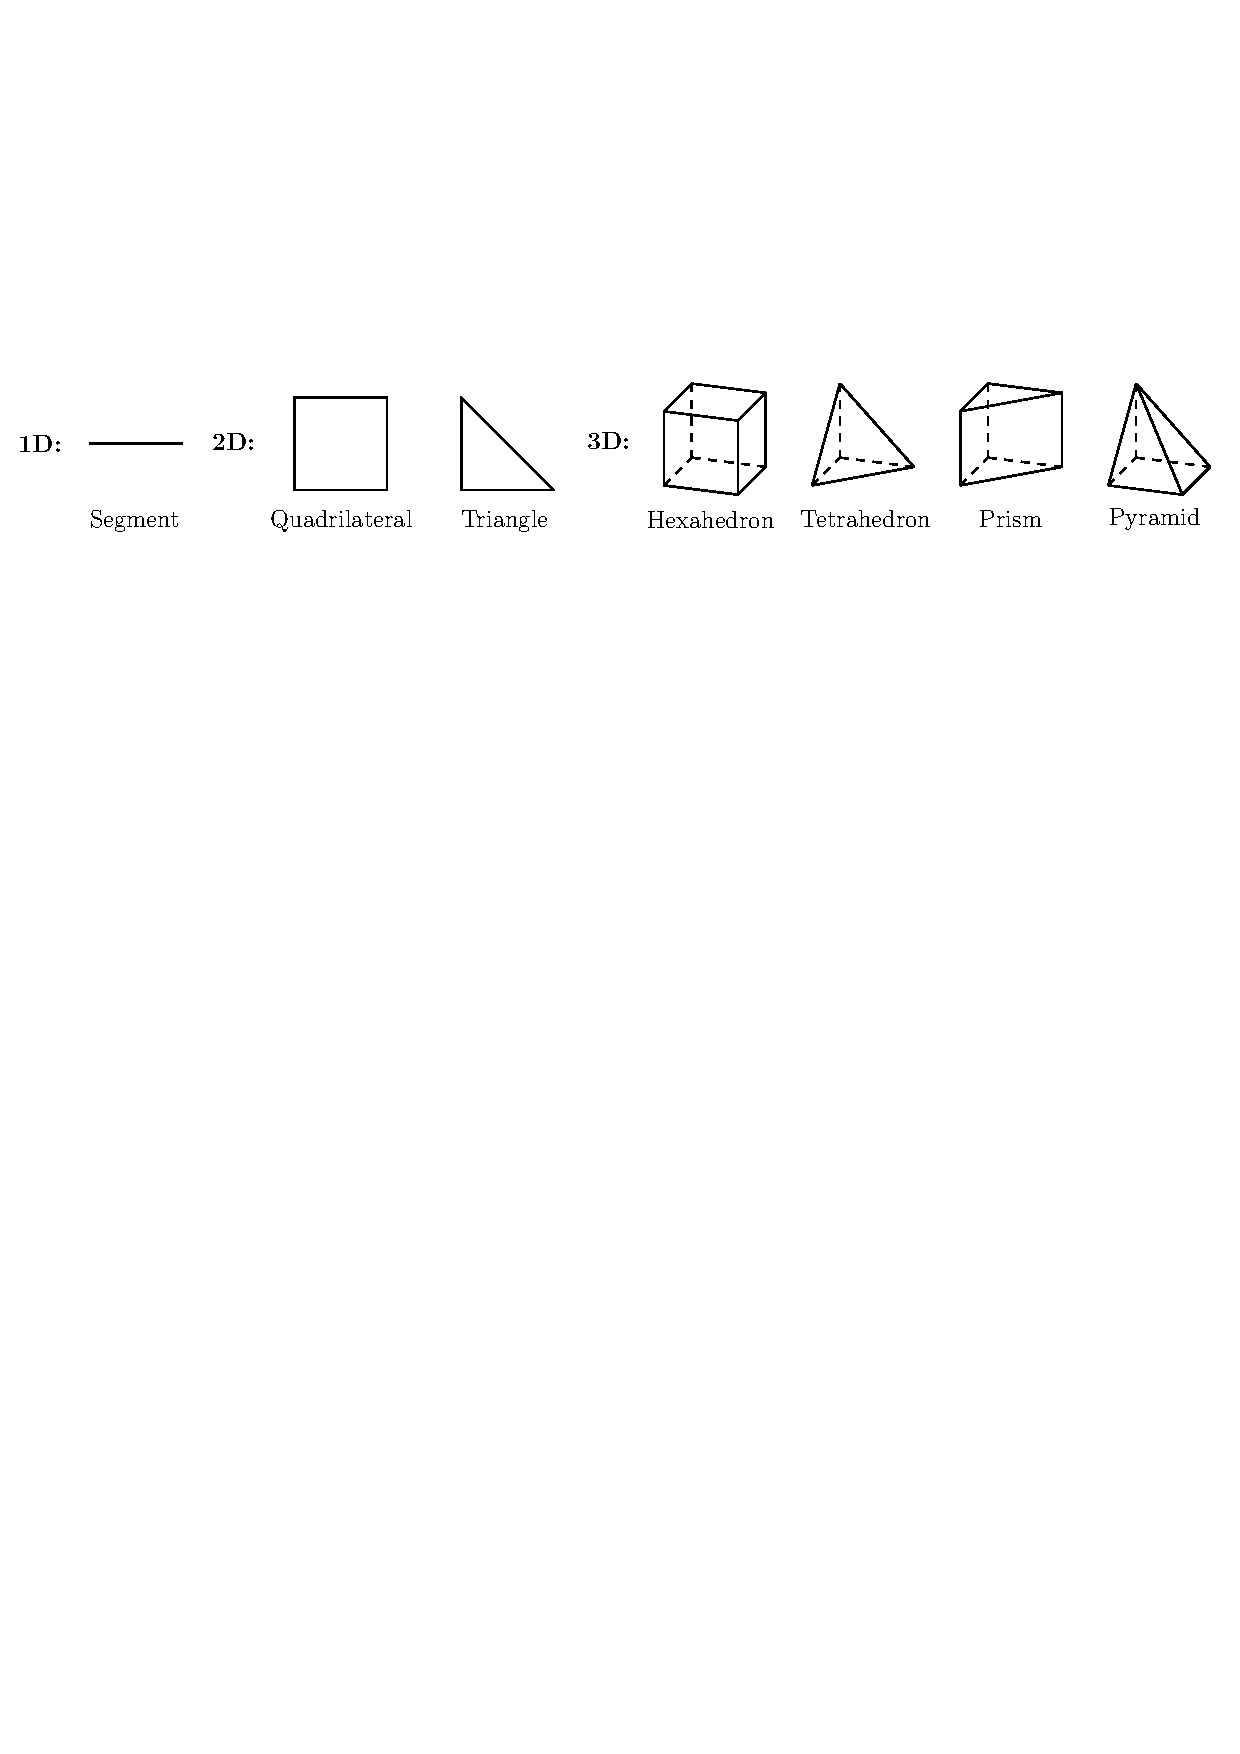
\includegraphics[scale=0.75]{./figures/ElementsAllShapes.pdf}
\caption{Elements of ``all shapes''.}\label{fig:elementsallshapes}
\end{center}
\end{figure}

There are many ways to construct sets of shape functions satisfying the aforementioned properties.
%We remind the reader that the performance of shape functions depends upon the particular problem being solved. % Therefore, there is no optimal or unique condition we may attribute to shape function construction in the generality preseneted in this paper.
However, we believe that in this work we have constructed a set which strikes an uncommon balance between simplicity and applicability. %\footnote{For instance, $H^1$ and $L^2$ shape functions for the triangle and tetrahedron which we derive are the same as those which appear in the work of \citet{Beuchler_Pillwein_Schoeberl_Zaglmayr_12} where they have shown good sparsity properties and also good conditioning for the stiffness and mass matrix.}
For all elements, and each associated energy space, we rely upon a simple methodology and a very small collection of ancillary functions to generate all of our shape functions.
Furthermore, we have supplemented this text with a package written in Fortran 90 defining each function presented in this work.\footnote{See the ESEAS library available at https://github.com/libESEAS/ESEAS.}
For these reasons, when reproducing our work in their own software, the readers should find the burden of implementation minimal.
We hope that our exposition will be clear and useful, particularly to those less familiar with the subject.

%This document presents a theory behind a stand alone package  that contains routines evaluating % Hereafter we will take freedom to use Finite Element (FE) jargon referring frequently to hexas and tets.

%The targeted audience for this document is less the colleagues contributing to the subject, who know it very well, but more a general computational science audience that may not be familiar with subtle mathematical details.
% We take thus some place not only to present specific constructions but also motivate them and place in a larger context. Throughout the document, we will not use boldface notations for 2D or 3D vectors (or vector-valued functions). These should be deduced from the context in which they are used.

For those at the forefront of shape function construction, we hope that our work will be intriguing if only for the elegance of our construction.
Particularly, we evidence \S\ref{sec:Pyramid} on pyramid shape functions.
The higher order discrete commuting exact sequence for this element appeared only recently in the work of \citet{Nigam_Phillips_11}.
Our construction for the pyramid presents shape functions spanning each of their discrete energy spaces while maintaining compatibility with the other 3D elements.
%With regards to $H(\mathrm{div})$, we believe this is the first construction presented in the literature which respects those pyramid higher order spaces.
We also remark that, for any given mesh, our shape functions are fully compatible across adjacent interelement boundaries due to considering so-called orientation embeddings.
Hence, no alterations of the shape functions are necessary at the finite element assembly procedure.
% orientation embedding (see \S\ref{sec:introorientations} for a more detailed discussion).
%With regard to attaining full compatibility of the shape functions across adjacent interelement boundaries via orientation embeddings, 
%we remark that our construction is able handle these coordinate transformations almost effortlessly by simply permuting the entries of a few relevant functions.
Moreover, these orientation embeddings are handled almost effortlessly by simply permuting the entries of a few relevant functions.
%We also evidence the ease at which orientation embeddings are handled in the shape function we present. 
% We believe that our presentation comprehensively illustrates the geometric similarities in each of the elements of ``all shapes.''

With regard to the choice of geometry (shape and size) of master elements, we followed \citet{hpbook}.
However, one of the key points is that our construction naturally applies to any other choice of master element geometries.
%However, we note that our methods are robust enough to easily generalize to other master element geometries.
%Despite basing our shape functions on the geometry (shape and size) of master elements followed by \citet{hpbook},
Other specific choices we made when enumerating element vertices, edges, and faces, can also be modified with little effort to the preferences of the reader.
%Of course, this also holds true for any other specific choices we made when enumerating element vertices, edges, and faces, which if desired, can be modified with little effort.
% and this particular choice of geometry is exploited in our construction.
%We also make specific choices when enumerating element vertices, edges, and faces, and also when selecting local edge and face orientations.
%If desired, these

For completeness, we have chosen to thoroughly verify the mathematical properties and to give a sound geometrical interpretation of our constructions rather than only give the necessary shape functions to the reader.
We concede that due to the depth of our presentation, and the expanse of our coverage, our offense lies only in the length of this document.
However, in a sense, an abridged version of this work is already present in a set of tables summarizing all the shape functions.
These can be conveniently consulted in Appendix~\ref{app:ShapeFunctionTable}. %to appear shortly for those requiring less details in the mathematics.

 %Our specific choices are summarized in Appendix \ref{app:Enumeration}.


%\subsection{Preliminaries}

\subsection{Energy Spaces and Exact Sequences}
\label{sec:Exactsequences}
Let $\Omega\subseteq\mathbb{R}^N$, with $N=1,2,3$ be a domain.
One arrives naturally at the \textit{energy spaces} $H^1(\Omega)$, $H(\text{curl},\Omega)$, $H(\text{div},\Omega)$ and $L^2(\Omega)$ in context of various variational formulations, see e.g. Chapter 1 in \citet{hpbook2}, \citet{DemkowiczGopalakrishnan13_2} and \citet{DemkowiczClosedRange}.
Along with operations of gradient, curl and divergence (understood in the sense of distributions), these spaces form the so-called \textit{complexes}, i.e. the composition of any two operators in the sequence reduces to the trivial operator.
The 1D complex, where $\Omega\subseteq\R$, provides the simplest example:
\begin{equation*}
	\mathbb{R} \stackrel{\text{id}}{\longrightarrow} H^1(\Omega) \stackrel{\nabla}{\longrightarrow} L^2(\Omega)
	\stackrel{0}{\longrightarrow} \{ 0 \}\,.
	\label{eq:1D_exact_sequence}
\end{equation*}
%where $\Omega = (0,1)$.
Here, the symbol $\mathbb{R}$ denotes constant functions, and $\{0\}$ is the trivial vector space consisting of the zero function only. By using the name of \textit{complex}, we communicate two simple facts: a) the derivative of a constant function is zero, and b) the composition of derivative (in fact, any linear operator) with the trivial (zero) operator is trivial as well. Equivalently, we can express the same facts by using null spaces and ranges of the involved operators:
\begin{equation*}
	\mathsf{R}(\text{id}) \subseteq \mathsf{N}(\nabla) \quad \text{and} \quad
	\mathsf{R}(\nabla) \subseteq \mathsf{N}(0) \, .
\end{equation*}
If instead of inclusions above, we have equalities, then we say that the complex (sequence) is \textit{exact}. This is indeed the case for the simply connected domain $\Omega = (0,1)$. 
By using the name \textit{exact sequence}, we communicate more information: a) the derivative of a function is zero \textit{if and only if} the function is a constant, and b) the function $\nabla : H^1(\Omega) \to L^2(\Omega)$ is a surjection (onto). From now on, we remove mention of the first and final terms of the exact sequence. The two spaces $\mathbb{R}$ and $\{0\}$, and the operators $\text{id}$ and $0$, are always assumed to buttress each of the sequences we later present. Moreover, whenever possible, we absorb the $\Omega$ assignment within the notation of each energy space. The domain $\Omega$ will always be assumed to be a simply connected domain in the relevant $\R^N$.
% It is customary to simplify the notation and drop the first and last spaces along with the identity and trivial operators, with their presence understood implicitly. We then have the 1D exact sequence:

\paragraph{1D Exact Sequence.} We now present the first exact sequence of simply connected domains in $\R$:
% \begin{description}
%   \item[1D sequence:]
\begin{equation}
H^1 \stackrel{\nabla}{\longrightarrow} L^2\, .
\end{equation}
% \end{description}

\paragraph{2D Exact Sequence.} The exact sequence for simply connected domains in $\R^2$ is of the form
\begin{equation}
H^1 \xrightarrow{\,\,\nabla\,\,} H(\mathrm{curl}) \xrightarrow{\nabla\times} L^2 \,,
\label{eq:2DExactSeq}
\end{equation}
where $\nabla\times$ and $\times$ are understood in two dimensions:
\begin{equation}
    \nabla\times E=\nabla\times\begin{pmatrix}E_1\\E_2\end{pmatrix}
        =\frac{\partial E_2}{\partial \xi_1}-\frac{\partial E_1}{\partial \xi_2}\,,\qquad\quad
    E\times F=\begin{pmatrix}E_1\\E_2\end{pmatrix}\times\begin{pmatrix}F_1\\F_2\end{pmatrix}
        =E_1 F_2 - E_2 F_1\,.\label{eq:2Dcurlandcross}
\end{equation}
By ``rotating'' $H(\mathrm{curl})$, the space $H(\mathrm{div})$ arises naturally:
\begin{equation}
    H(\mathrm{div})=\Big\{V_E=\Big(\begin{smallmatrix}0&1\\[2pt]-1&0\end{smallmatrix}\Big)E=
        \Big(\begin{smallmatrix}E_2\\-E_1\end{smallmatrix}\Big):
            E=\Big(\begin{smallmatrix}E_1\\E_2\end{smallmatrix}\Big)\in H(\mathrm{curl})\Big\}\,.
\label{eq:Hdiv2Ddef}
\end{equation}
Defined in this way, the ``rotated'' exact sequence is immediately satisfied:
\begin{equation}
H^1 \xrightarrow{\mathrm{curl}} H(\mathrm{div}) \xrightarrow{\,\nabla\cdot\,} L^2 \,,
\label{eq:2DExactSeqRotated}
\end{equation}
where, for all $\phi\in H^1$ and all $E\in H(\mathrm{curl})$, the operations satisfy the following relations: %$\mathrm{curl}\,(\phi)$ is understood as
\begin{equation}
    \mathrm{curl}\,(\phi)=\begin{pmatrix}\frac{\partial\phi}{\partial \xi_2}\\[4pt]-\frac{\partial\phi}{\partial \xi_1}\end{pmatrix}
        =\begin{pmatrix}0&1\\[4pt]-1&0\end{pmatrix}\nabla\phi\,,\qquad\quad
            \nabla\cdot V_E=\nabla\cdot\begin{pmatrix}0&1\\[4pt]-1&0\end{pmatrix}E=\nabla\times E\,.
\end{equation}


% For a simply connected domain, $\Omega \subset \mathbb{R}^2$, we have two exact 2D sequences:
% % \begin{description}
%   % \item[2D sequence:]
% \be
% H^1(\Omega) \stackrel{\bfnab}{\longrightarrow}
% H(\text{curl},\Omega) \stackrel{\text{curl}}{\longrightarrow}
% L^2(\Omega) \, ,%\quad \text{and,}
% \label{eq:2D_exact_sequence}
% \ee
%   % \item[Rotated 2D sequence:]
% and its rotated analogue,
% \be
% H^1(\Omega) \stackrel{\bfnab \times }{\longrightarrow}
% H(\text{div},\Omega) \stackrel{\bfnab \cdot}{\longrightarrow}
% L^2(\Omega) \, .
% \label{eq:2D_rotated_exact_sequence}
% \ee
% % \end{description}
% The operators curl and $\bfnab \times$ seen above are defined as follows:
% \be
% \text{curl} (E_1(x_1,x_2),E_2(x_1,x_2)) = \frac{\ptl E_2}{\ptl x_1} - \frac{\ptl E_1}{\ptl x_2}
% \quad \text{and} \quad
% \bfnab \times u(x_1,x_2) = \left(
% \frac{\ptl u}{\ptl x_2}, - \frac{\ptl u}{\ptl x_1} \right) \ .
% \label{eq:2D_curl_operators}
% \ee
% It is easy to see that the rotated sequence is obtained from the original one by rotating the coordinates,
% $(x_1,x_2)\mapsto(x_2,-x_1)$. The main point of the rotated sequence is that there is no need for a separate
% construction of 2D $H(\text{div})$ shape functions that can be obtained from 2D $H(\text{curl})$ shape functions
% by using the formula:
% \be
% (V_1,V_2) = (E_2, - E_1) \, .
% \ee
\paragraph{3D Exact Sequence.} Finally, for a simply connected domain in $\mathbb{R}^3$, we have the 3D exact sequence
\begin{equation}
H^1 \xrightarrow{\,\,\nabla\,\,} H(\mathrm{curl}) \xrightarrow{\nabla\times} H(\mathrm{div}) \xrightarrow{\,\nabla\cdot\,} L^2 \, .
\label{eq:3D_exact_sequence}
\end{equation}
%Note that the 2D exact sequences are ``embedded'' in the 3D sequence if one considers the appropriate restriction to functions of only two variables.

For all elements, these exact sequences will be reproduced on the discrete level by replacing the energy spaces with appropriate polynomial subspaces.\footnote{Or rational polynomial subspaces in the case of the pyramid (see \S\ref{sec:Pyramid}).} We shall use the standard notation:
\begin{equation}
\begin{aligned}
	\text{1D}:&\quad\qquad W^p \xrightarrow{\,\,\nabla\,\,\,}Y^p \, ,\\
	\text{2D}:&\qquad\!\!\Bigg\{\begin{array}{c}
		W^p \xrightarrow{\,\,\nabla\,\,\,} Q^p \xrightarrow{\nabla\times} Y^p  \, ,\\[4pt]
		W^p \xrightarrow{\mathrm{curl}} V^p \xrightarrow{\,\nabla\cdot\,} Y^p  \, ,\end{array}\\
	\text{3D}:&\quad\qquad W^p \xrightarrow{\,\,\nabla\,\,\,} Q^p \xrightarrow{\nabla\times} V^p \xrightarrow{\,\nabla\cdot\,} Y^p\,.
\end{aligned}
\label{eq:polynomial_exact_sequences}
\end{equation}
The symbol $p$ loosely denotes the polynomial order and should not be interpreted literally.\footnote{By this we mean that $p$ should, in fact, be interpreted as a multi-index for the Cartesian product elements.}

In this work, we shall consider only spaces of the \textit{first type} which, with the exception of the pyramid, were introduced by \citet{Nedelec80} in the \textit{first} of his two famous papers.
The pyramid spaces were taken as the first set of spaces proposed by \citet{Nigam_Phillips_11}.
All these spaces satisfy a number of fundamental properties.
First, the spaces of the different elements are said be tracewise \textit{compatible} at the level of spaces.
This allows them to be used in \textit{hybrid meshes}, which may contain elements of all shapes.
Second, for each element, $W^p$ contains polynomials of total order $p$, while $Q^p$, $V^p$ and $Y^p$ contain polynomials of total order $p-1$, meaning that the overall drop in polynomial degree from the first discrete energy space in the exact sequence to the last discrete energy space is one.
%That is, if the space $W^p$ contains polynomials of order $p$, then $Y^p$ contains polynomials of order $p-1$.
Thirdly, for a given element and energy space, the discrete spaces form a nested sequence of spaces as the order increases (for instance, $W^p\subseteq W^{p+1}$ and so on).
This is a necessary condition for the construction of hierarchical sets of shape functions.
Lastly, the spaces form \textit{commuting} exact sequences for each element.
This, coupled with the previous properties, ensures (global) interpolation estimates for \textit{all} of our energy spaces subject to affine transformations of the master element geometries \citep{monk_demkowicz}.

%With an outlook toward {\em hybrid meshes} that may contain elements of all shapes in one mesh, we require the spaces of the different elements to be tracewise \textit{compatible} at the level of spaces.
%Moreover, another desired property is that they form \textit{commuting} exact sequences for each element.
%This then ensures (global) interpolation estimates for \textit{all} of our energy spaces subject to affine transformations \citep{monk_demkowicz}.
%Finally, the discrete energy spaces (for a given element) should form a nested sequence of spaces as the order increases (for instance, $W^p\subseteq W^{p+1}$ and so on).
%This is a necessary condition for the construction of hierarchical sets of shape functions.
%In this work, all these properties are satisfied.
%We shall consider only spaces of the {\em first type} which, with the exception of the pyramid, were introduced by \citet{Nedelec80} in the {\em first} of his two famous papers.
%They present an overall drop in polynomial degree by one from the first discrete energy space in the exact sequence to the last discrete energy space.
%That is, if the space $W^p$ contains polynomials of order $p$, then $Y^p$ contains polynomials of order $p-1$.

%With these properties in mind, in this work  
%%The use of these spaces, is motivated with an outlook toward {\em hybrid meshes} that may contain elements of all shapes in one mesh.
%%To have such a mesh, the spaces of the different elements have to ``understand'' each other across the element boundaries.
%%If this is the case, they are said to be tracewise \textit{compatible} at the level of spaces.
%A common property of all these spaces is an overall drop in polynomial degree by one from the first discrete energy space in the exact sequence to the last discrete energy space.
%That is, if the space $W^p$ contains polynomials of order $p$, then $Y_p$ contains polynomials of order $p-1$.
%Moreover, another shared fundamental property is that they form \textit{commuting} exact sequences.
%This then ensures (global) interpolation estimates for \textit{all} of our energy spaces subject to affine transformations \citep{monk_demkowicz}.
%Finally, it is noted that the discrete energy spaces (for a given element) form a nested sequence of spaces as the order increases (for instance, $W^p\subseteq W^{p+1}$ and so on).
%This is a necessary condition for the construction of hierarchical sets of shape functions.

%the $H(\text{curl})$ and $H(\text{div})$ conforming N\'{e}d\'{e}lec and Raviart-Thomas spaces present in the exact sequences of the triangle and tetrahedral elements have the nice property that they are affine invariant.

%The second aspect of the exact sequence philosophy is a careful choice of discrete energy spaces. In our discrete exact sequences for the triangle and tetrahedral elements, we use the well known $H(\text{curl})$-conforming \Nedelec~and $H(\text{div})$-conforming Raviart-Thomas spaces.\footnote{See definitions for these spaces in \S~\ref{sec:Tri} and \S~\ref{sec:Tet}.} Unlike other higher order discete energy spaces used in the literature, these spaces happen to be affine invariant while also preserving a commuting exact sequence structure. In fact, we make the distinction that all of our discrete exact sequences preserve a commuting exact sequence stucture which  \textit{cite}

%In the $p$ or $hp$ FE methods, the order of approximation may vary from element to element and it may be different for each relevant topological entity (edge, face or element interior).
%That is reflected in the constructions presented in this report.
%The edge order must not exceed the order of adjacent spaces and the face order must not exceed the order of adjacent elements (see \citet{hpbook} and \citet{hpbook2} for discussions on the {\em minimum rule}).

%Unlike in \citet{hpbook,hpbook2}, we do not account in our notation for discrete spaces for variable order.

\subsection{Shape Functions}
We shall always identify the discrete spaces first (like $W^p$, $Q^p$, $V^p$ and $Y^p$ in \eqref{eq:polynomial_exact_sequences}), and only afterward introduce the corresponding shape functions that provide bases for those spaces.
This is a good place to remind the reader that there are, in fact, two competing schools of thought when it comes to the theory of shape functions.

%The classical definition of \citet{Ciarlet} starts with \textit{degrees of freedom} that are functionals defined on some large energy space $\mathcal{X}$ (like $H^1$).
The classical definition of \citet{Ciarlet} starts with \textit{degrees of freedom} that are functionals defined on some large subset $\mathcal{X}$ of an energy space $U$ (like $C^\infty\cap H^1\subseteq H^1$). 
The shape functions, which are elements spanning some discrete (finite dimensional) space $X\subseteq\mathcal{X}$ (e.g. $W^p\subseteq C^\infty\cap H^1$), are then defined as the dual basis to the linearly independent (when restricted to $X$) degrees of freedom.
An \textit{interpolation operator} from $\mathcal{X}$ to $X$ is then naturally defined.
In this construction, we must (usually) precompute the shape functions, e.g. in terms of combinations of monomials whose corresponding coefficients are stored.

%The classical definition of \citet{Ciarlet} starts with {\em degrees of freedom} that are functionals defined on some energy space $\mathcal{X}$ containing both the discrete trial space $X\subseteq\mathcal{X}$ and the exact solution. The degrees of freedom should be linearly independent when restricted to the finite dimensional domain $X$. The shape functions, which are elements of $X$, are then precisely the dual basis to the restricted degrees of freedom. An \textit{interpolation operator} is then intuitively defined. In this construction, we must (usually) precompute the shape functions in terms of combinations of monomials and then store the corresponding coefficients.

The competing approach of Szab\'o \citep{SzaboBabuska91} starts with a direct construction of shape functions by following a topological classification (of vertices, edges, faces and element interiors) induced by conformity requirements.
The shape functions are defined in terms of families of polynomials (e.g. Legendre) and their integrals, and are computed using simple recursive formulas. This is the approach taken in this work.
The so-called \textit{projection-based interpolation} \citep{hpbook,hpbook2} defined through local projections over element edges, faces and interior, is introduced \textit{independently} of the construction of shape functions.
Therefore, with no need to precompute coefficients defining the shape functions, following Szab\'o's approach is perhaps more convenient and straightforward.

\subsection{Hierarchy in \texorpdfstring{$p$}{p}}

Given an energy space (like $H^1$) and a conforming discrete space of order $p$ (like $W^p\subseteq H^1$), denote the shape functions forming a basis for the discrete space by $\mathcal{B}^p$ (e.g. $\mathrm{span}(\mathcal{B}^p)=W^p\subseteq H^1$). 
A construction is said to be hierarchical in $p$ if $\mathcal{B}^p\subseteq\mathcal{B}^{p+1}$ for all $p$, so that the set of shape functions spanning a space of a certain order is found in all subsequent enriched spaces of higher order.
This implies that as $p$ increases, all one has to do is to add a few functions to a smaller previously constructed set of shape functions.

%In our construction, hierarchy in the order $p$ of shape functions will be enforced.
%That is, the set of shape functions existing in a discrete energy space of a particular order (say $p$) will be found in all subsequent enriched discrete energy spaces of higher order, say $q\geq p$.
%For example, when constructing shape functions spanning $W^{p+1}$, all one needs to do is add a few functions to the smaller previously constructed set of shape functions which span $W^p$.
%%For example, let $p\geq1$ and let $W^p$ be the higher order discrete energy space conforming to $H^1$.
%%We will construct a set of shape functions spanning $W^{p}$ by simply adding to the smaller, previously constructed set of shape functions which span $W^{p-1}$.

In our construction, hierarchy in $p$ will be enforced. 
In a given mesh, it will allow comparison of shape functions between adjacent elements that have different order, so that at least some of the shape functions of the neighboring elements will match.
%More so, one can even have different orders for each topological entity (vertex, edge, etc.) independently.
This is crucial with regard to the notion of local $p$ adaptivity, which some methods employ.
In our work, this flexibility in the variability of the order will be partly reflected by the natural anisotropies present in Cartesian product elements, such as quadrilaterals, hexahedra and prisms, where each independent direction can have a different order.
More information can be consulted in the literature (see \citet{hpbook2} and references therein).


\subsection{Traces and Compatibility}
\label{sec:compatibility}
%Global conformity depends upon the energy space. More precisely, the requirements on the global continuity For instance, $H^1$-conforming shape functions must be globally continuous while the vector-valued $H(\text{curl})$-conforming shape functions must only be continuous in their tangential components across interelement boundaries. Similarly, for vector-valued $H(\text{div})$-conforming shape functions, only the continuity of only the normal component is enforced. In the final case, $L^2$-conformity does not involve any continuity assumptions at all.

%The global solution of any finite element method should satisfy certain conformity (continuity) properties, which clearly depend upon the energy space.
For a function to be contained in a given energy space it must satisfy some global conformity conditions which depend upon the space.
For instance, functions in $H^1$ are almost globally continuous, but functions in $L^2$ can be much more discontinuous.
%In the case of the vector valued $H(\mathrm{curl})$ and $H(\mathrm{div})$ spaces, there is a middle ground.

Due to these conformity requirements, each energy space has a different definition of \textit{trace} at the boundaries. 
%To be conforming to the energy space, functions should then be continuous at the trace level.
The different traces only make sense on certain parts of the boundary.
%and functions are said to be continuous at the trace level.
%This trace affects only certain parts of the boundary.
For instance, consider a polyhedral element.
%Polyhedral elementsthis means the functions should be (tracewise) continuous across interelement boundaries.
\begin{itemize}
	\item The $H^1$ trace is the value of the function itself at the boundary. In 3D, it may take values at element vertices, edges and faces which lie along the boundary.
	\item The $H(\text{curl})$ (tangential) trace is the tangential component of the vector valued function across the boundary. It may take values at edges and faces in the boundary, but not at vertices, since these do not have a concept of tangent. In fact, the $H(\text{curl})$ (tangential) trace is scalar valued across edges (which have 1D tangent spaces) and has two components across faces (which have 2D tangent spaces).
	\item The $H(\text{div})$ (normal) trace is the normal component of the vector valued function across the boundary. In 3D, it can take values at the faces of the boundary, but not at vertices or edges, since they do not have a unique notion of normal. In 2D, edges along the boundary \textit{do} have a notion of normal, so the (normal) edge trace does exist.
	\item There is no notion of trace for $L^2$.
\end{itemize}

%Different energy spaces also lead to different notion of {\em traces}. By the $H^1$ trace of a scalar-valued (sufficiently) regular function, we understand simply its restriction to the boundary. By the (tangential) $H(\text{curl})$ trace of a vector-valued function, we understand the restriction of its {\em tangential component} on the boundary. Thus, the  $H(\text{curl})$ trace of a two component function $(E_1,E_2)$ in $\mathbb{R}^2$ to an element edge, is going to be a scalar-valued function. In 3D, however, the trace of a 3D vector-valued function to an element face, will be a 2D vector. Similarly, the (normal) $H(\text{div})$ trace of a vector-valued function to an edge (2D) or a face (3D) is always a vector orthogonal to the element boundary that involves just one scalar component.

%Functions should then to be continuous at the trace level to .
At the discrete level, these considerations lead naturally to a classification of shape functions according to topological entities, which in turn depend on the number of spatial dimensions:
\begin{equation*}
	\begin{aligned}
		\text{1D:}&\quad\qquad\text{vertex and edge shape functions,}\\
		\text{2D:}&\quad\qquad\text{vertex, edge, and face shape functions,}\\
		\text{3D:}&\quad\qquad\text{vertex, edge, face and interior shape functions.}
	\end{aligned}
\end{equation*}

For any given mesh and energy space, shape functions of adjacent elements \textit{must} be continuous at the trace level across the shared interelement boundaries.
This is referred to as \textit{compatibility}, and results in the global conformity of the (disjoint union of) shape functions. 
For instance, in 2D, the order $p$ edge shape function of a quadrilateral would need to be compatible with the order $p$ edge shape function of an adjacent triangle (see Figure \ref{fig:compatibilitydefinition}).

\begin{figure}[!ht]
\begin{center}
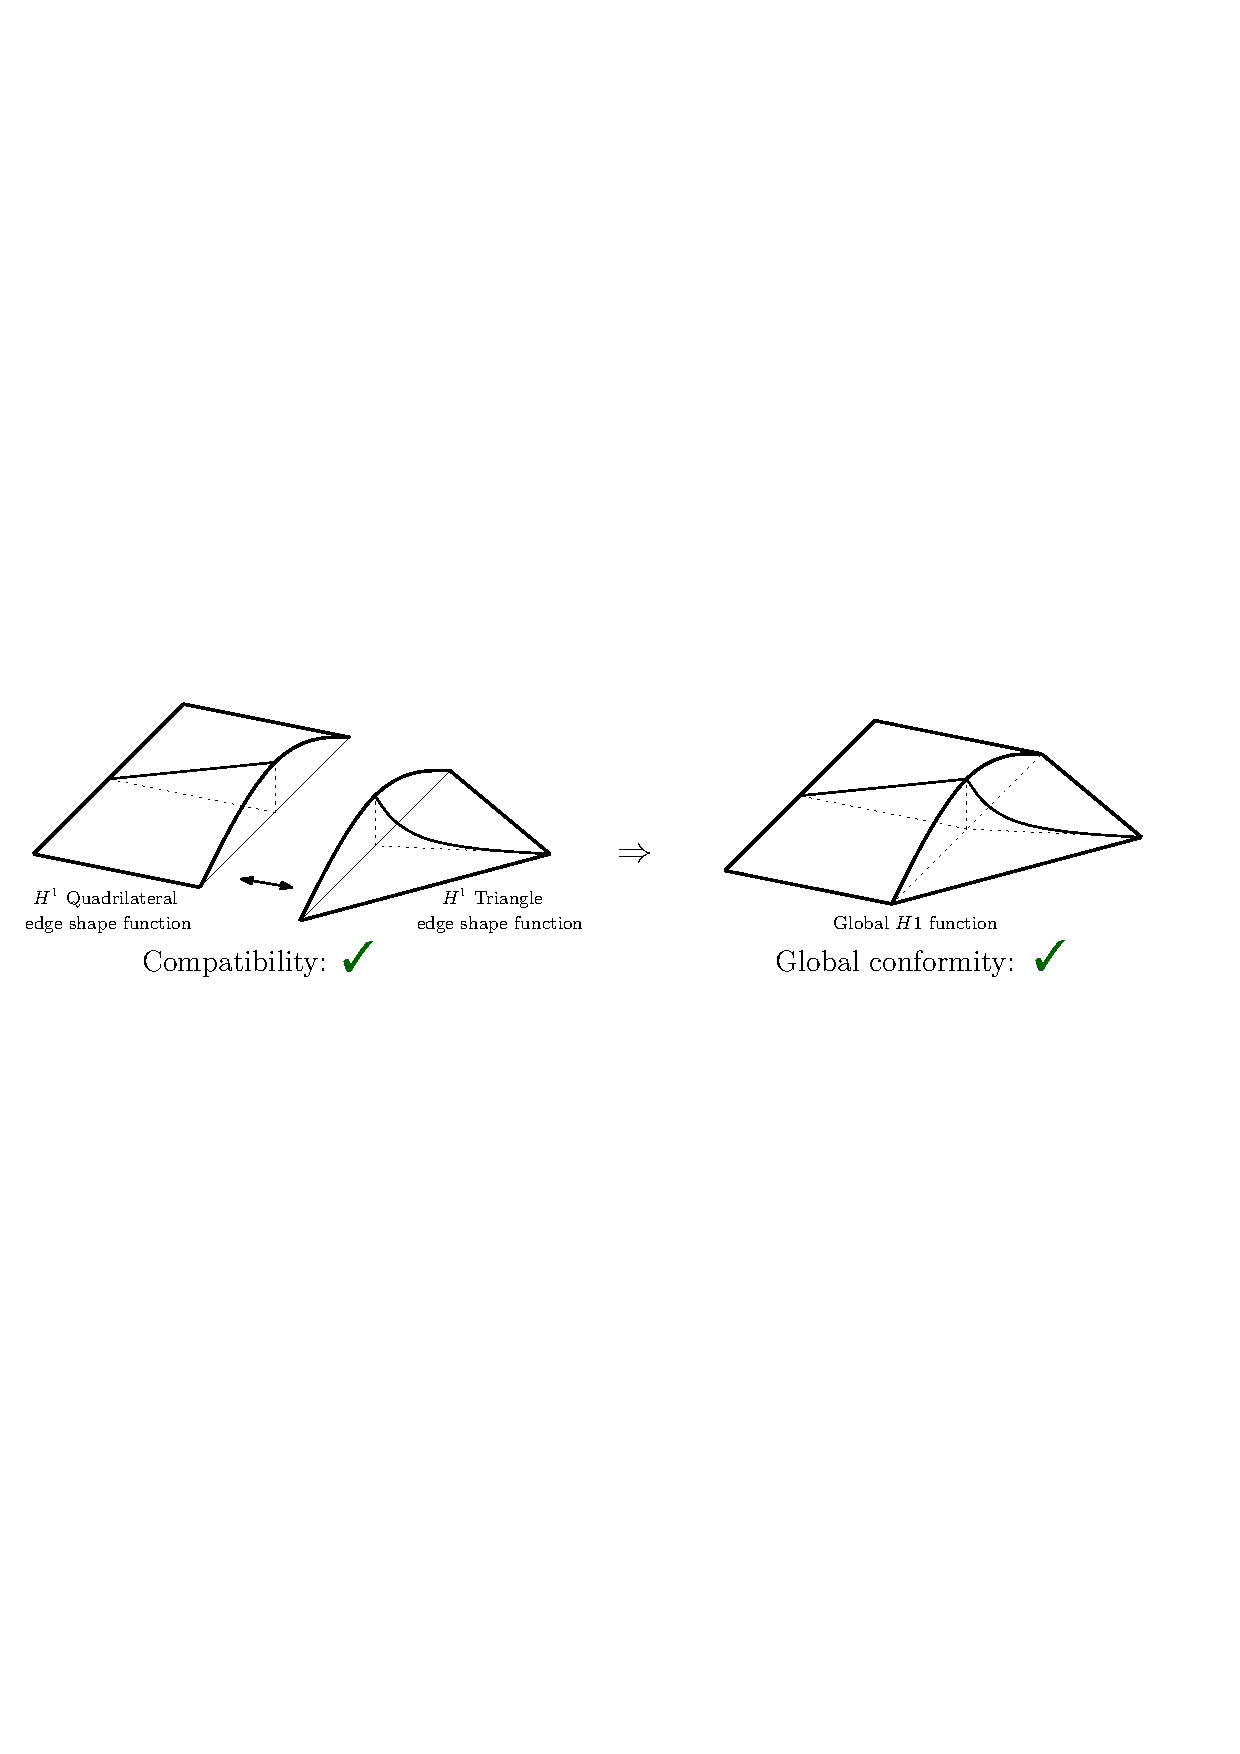
\includegraphics[scale=0.7]{./figures/CompatibilityDefinition.pdf}
\caption{Example of compatible $H^1$ edge functions resulting in a globally conforming $H^1$ function.}
\label{fig:compatibilitydefinition}
\end{center}
\end{figure}

% To be (globally) conforming to a certain energy space, shape functions of adjacent elements should be continuous at the trace level across the shared interelement boundaries.
% This is referred to as \textit{compatibility}.
% For instance, in 2D, an order $p$ edge shape function of a quadrilateral should be compatible with the order $p$ edge shape function of an adjacent triangle.
%In order for this to be possible, shape functions related to a given entity have to satisfy certain trace properties.
%The shape functions related to a given entity have to satisfy certain trace properties to ensure that they are \textit{compatible} (continuous at the trace level) with other shape functions from adjacent elements (related to the same entity).
%These properties are explained next.

\subsection{Embedded Sequences and Dimensional Hierarchy}
\label{sec:dimensionalhierarchy}

To enforce compatibility, it is useful to actually begin with a known trace over the (shared) boundary and then extend (or lift) it to the rest of the element.
This is the approach inherently present in our constructions.
In fact, this idea is reinforced when looking at the exact sequences.
%Next is a fundamental observation regarding exact sequences and the number of spatial dimensions:
Note the crucial fact that the lower dimensional sequences are ``embedded'' in the higher dimensional sequences if one considers the appropriate restrictions.
This is better represented by the following diagram,
\begin{equation}
	\begin{gathered}
  %\text{2D:}&\qquad H^1 \xrightarrow{\,\,\nabla\,\,} H(\mathrm{curl}) \xrightarrow{\nabla\times} L^2 \\
  %\text{1D:}&\qquad H^1 \xrightarrow{\,\,\nabla\,\,} L^2\,.
  	\xymatrix{
        {\text{3D:}} & H^1 \ar[r]^{\nabla\,\,\,\,} \ar@{.>}[d]^{\mathrm{tr}} & H(\mathrm{curl})
          \ar[r]^{\,\,\,\nabla\times} \ar@{.>}[d]^{\mathrm{tr}} & H(\mathrm{div})
          	\ar[r]^{\,\,\,\nabla\cdot} \ar@{.>}[d]^{\mathrm{tr}} & L^2\\
        {\text{2D:}} & H^1 \ar[r]^{\nabla\,\,\,} \ar@{.>}[d]^{\mathrm{tr}} & H(\mathrm{curl})
          \ar[r]^{\,\,\,\nabla\times} \ar@{.>}[d]^{\mathrm{tr}} & L^2\\
        {\text{1D:}} & H^1 \ar[r]^{\nabla\,\,\,\,} & \,\,\,\,L^2\,,\, }
	\end{gathered}\label{eq:traceexactsequences}
\end{equation}
where the ``mapping arrows'', $\xymatrix{{}\ar@{.>}[r]^{\mathrm{tr}}&{}}$, indicate that the range (of the trace) is actually a larger space.
These arrows are meant to be motivational only.
At the discrete level, we always reproduce the above diagram precisely with the dotted lines being replaced by well defined maps.

Indeed, we will enforce a \textit{dimensional hierarchy} through traces which is consistent with the previous discussion.
The template for this new form of hierarchy is precisely \eqref{eq:traceexactsequences}, but it is satisfied at the level of the shape functions themselves (not only the spaces).
One will begin the construction by first defining the 1D shape functions (over the segment), then defining all the 2D functions (over the quadrilateral and triangle), and finish with the 3D shape functions.
%Throughout the construction, through the trace operation, the shape functions should be nested % (e.g. the trace of a 2D $H^1$ edge function, restricted to the corresponding edge, will produce a 1D $H^1$ function).
%and therefore, all higher dimensional shape functions are actually extensions of lower dimensional ones.
Throughout the construction, the higher dimensional shape functions will have as (nonzero) trace a lower dimensional function,
so that they are actually extensions of these lower dimensional functions.
Indeed, the shape functions are nested through the trace operation at each topological entity lying in the boundary.

For example, given an edge of a 2D element, the nonzero edge traces of the 2D $H^1$ shape functions should reproduce the 1D $H^1$ shape functions.
Hence, some 2D $H^1$ shape functions are said to be extensions of the 1D $H^1$ shape functions.
Similarly, the nonzero edge trace of 2D $H(\mathrm{curl})$ shape functions should be the 1D $L^2$ shape functions (see \eqref{eq:traceexactsequences}).
These relations hold per topological entity as well.
For example, the nonzero edge trace of 2D $H^1$ \textit{vertex} functions should coincide with the 1D $H^1$ \textit{vertex} functions, and the nonzero trace of the 2D $H^1$ \textit{edge} functions should coincide with the 1D $H^1$ \textit{edge} functions (see Figures \ref{fig:2Dvertexcompatibility} and \ref{fig:2Dedgecompatibility} later on).
%The 1D trace of the 2D $H^1$ \textit{face} functions will be zero.
When enforced, these nice relationships not only aid in the compatibility, but, from the computational standpoint, have the benefit of allowing us to recycle a large amount of code when moving from one element construction to another.
%This implies, for example, that 2D $H^1$ edge functions are extensions (to the quadrilateral or triangle) of known 1D (segment) $H^1$ edge functions.
%Similarly, 2D $H(\mathrm{curl})$ edge functions are extensions of known 1D $L^2$ edge functions.
%Regarding the number of components, this is possible because the 2D $H(\mathrm{curl})$ (tangential) \textit{trace} only has one component.
%This will be clearer when the shape functions are actually constructed.

\subsection{Basic Properties of Shape Functions}

In this section we will describe the basic properties that our shape functions should satisfy.
These properties are specific to the topological entity (vertices, edges, faces, interior) and the energy space to which the shape functions are associated.
For example, vertex functions satisfy different properties than edge functions in $H^1$, and 2D edge functions satisfy different properties in $H^1$ and $H(\mathrm{curl})$.

%The number of shape functions related to a given topological entity is different.
%Generally speaking, 
For a given element and energy space, each topological entity owns a set of shape functions, which is said to be \textit{associated} to the entity.
These functions are nonzero at the associated topological entity.
Indeed, each vertex is associated to \textit{one} $H^1$ vertex shape function.
Meanwhile, each edge, face, and interior of the element is associated to a \textit{set} of edge, face, and interior shape functions of size of the order of $p$, $p^2$ and $p^3$ respectively.
%The functions are nonzero at the associated topological entity.
For example, in $H^1$, each edge is associated to a set of $p-1$ edge shape functions.
 %(and the same holds for $H(\mathrm{curl})$). 
%while each face is associated to sets of $H^1$, $H(\mathrm{curl})$ and $H(\mathrm{div})$ face shape functions, each having about $p^2$ functions.
%Moreover, for a given energy space, each edge, face, and interior of the element is associated to a \textit{set} of edge, face, and interior shape functions with size on the order of $p$, $p^2$ and $p^3$ respectively. 
%That is, there are around $p$ shape functions associated to every edge
%\footnote{Here, again we are being liberal in the use of $p$, which loosely denotes the polynomial order. In fact, $p$ is a multi-index for the quadrilateral, hexahedron and prism.}

Now, for a given dimension, space, and topological entity, we will cover three main aspects of the shape functions.
First, are the vanishing properties that they should satisfy.
These properties establish a form of trivial compatibility along some parts of the boundary.
Functions whose trace vanishes everywhere along the boundary are called \textit{bubbles}, and they are trivially compatible with each other.
Second, come the nonzero trace properties.
These are, in general, nontrivial, and ensure either full compatibility or compatibility modulo ``orientations'' (see \S\ref{sec:introorientations} for a discussion on ``orientations'').
Fortunately, dimensional hierarchy will determine the form of these nonzero traces.
Third, are some properties that the shape functions should satisfy along the element itself in order to have hierarchy in $p$.


%Throughout this description, the aspect of dimensional hierarchy through traces will be seen to be extremely practical (if not fundamental) in satisfying the compatibility of the shape functions.
%Next, we present the required trace properties, along with a more detailed view of the whole logic of the construction.
%As discussed above, the construction will enforce both the typical hierarchy in order $p$ and the dimensional hierarchy through traces.

\subsubsection{1D}

In one dimension, classification of shape functions is:
\begin{align*}
  H^1:&\quad\text{vertex and edge functions,}\\
  L^2:&\quad\text{\phantom{vertex and} edge functions.}
\end{align*}
There is only one simply connected 1D element, which is the segment (or edge), and its boundary is just its two vertices.
%Each of the (two) vertices is related to \textit{one} vertex shape function.
%The edge is associated to a set of edge functions.

\paragraph{$H^1$.}
\textit{Vertex functions:} %Consider the vertex functions.
First, there are the vanishing properties.
The vertex functions should vanish at the other (unassociated) vertex.
Second, there are the nonzero trace properties.
The vertex functions should take the value $1$ at the associated vertex.
This will ensure \textit{full} compatibility in 1D.
%This is enough to satisfy compatibility across interelement boundaries in one dimension.
Third, there is the form of the function itself.
There are multiple ways in which the vertex function can decay towards the other vertex (see Figure \ref{fig:vertexcompatibility}).
%This is referred to as \textit{vertex blending across the edge}. %, and is a concept that becomes more important when satisfying compatibility at higher spatial dimensions.
If the hierarchy in $p$ is not an issue, the decay could be nonlinear and dependent on $p$, and this may have some computational advantages.
For example, when having a mesh with uniform order $p$ across all elements, this nonlinear decay might lead to a better conditioning of finite element matrices.
%Despite this, depending on the order $p$ of the element, the blending could be chosen as nonlinear.
%This would destroy the hierarchy in $p$, but could lead to some advantages, such as better conditioning of finite element matrices.
%When having a mesh with uniform order $p$ across all elements, this could be a useful asset, but the notion of $p$ adaptivity, which requires hierarchy in $p$, is important to us.To maintain hierarchy in $p$, this decay is chosen as linear in this work.
However, as mentioned before, we want our shape functions to be useful in $p$ adaptive environments in higher dimensions.
Hence, we enforce hierarchy in $p$, and this restricts our choice to $p=1$, so the decay must be linear.
Indeed, this is the typical and simplest choice.

\begin{figure}[!ht]
\begin{center}
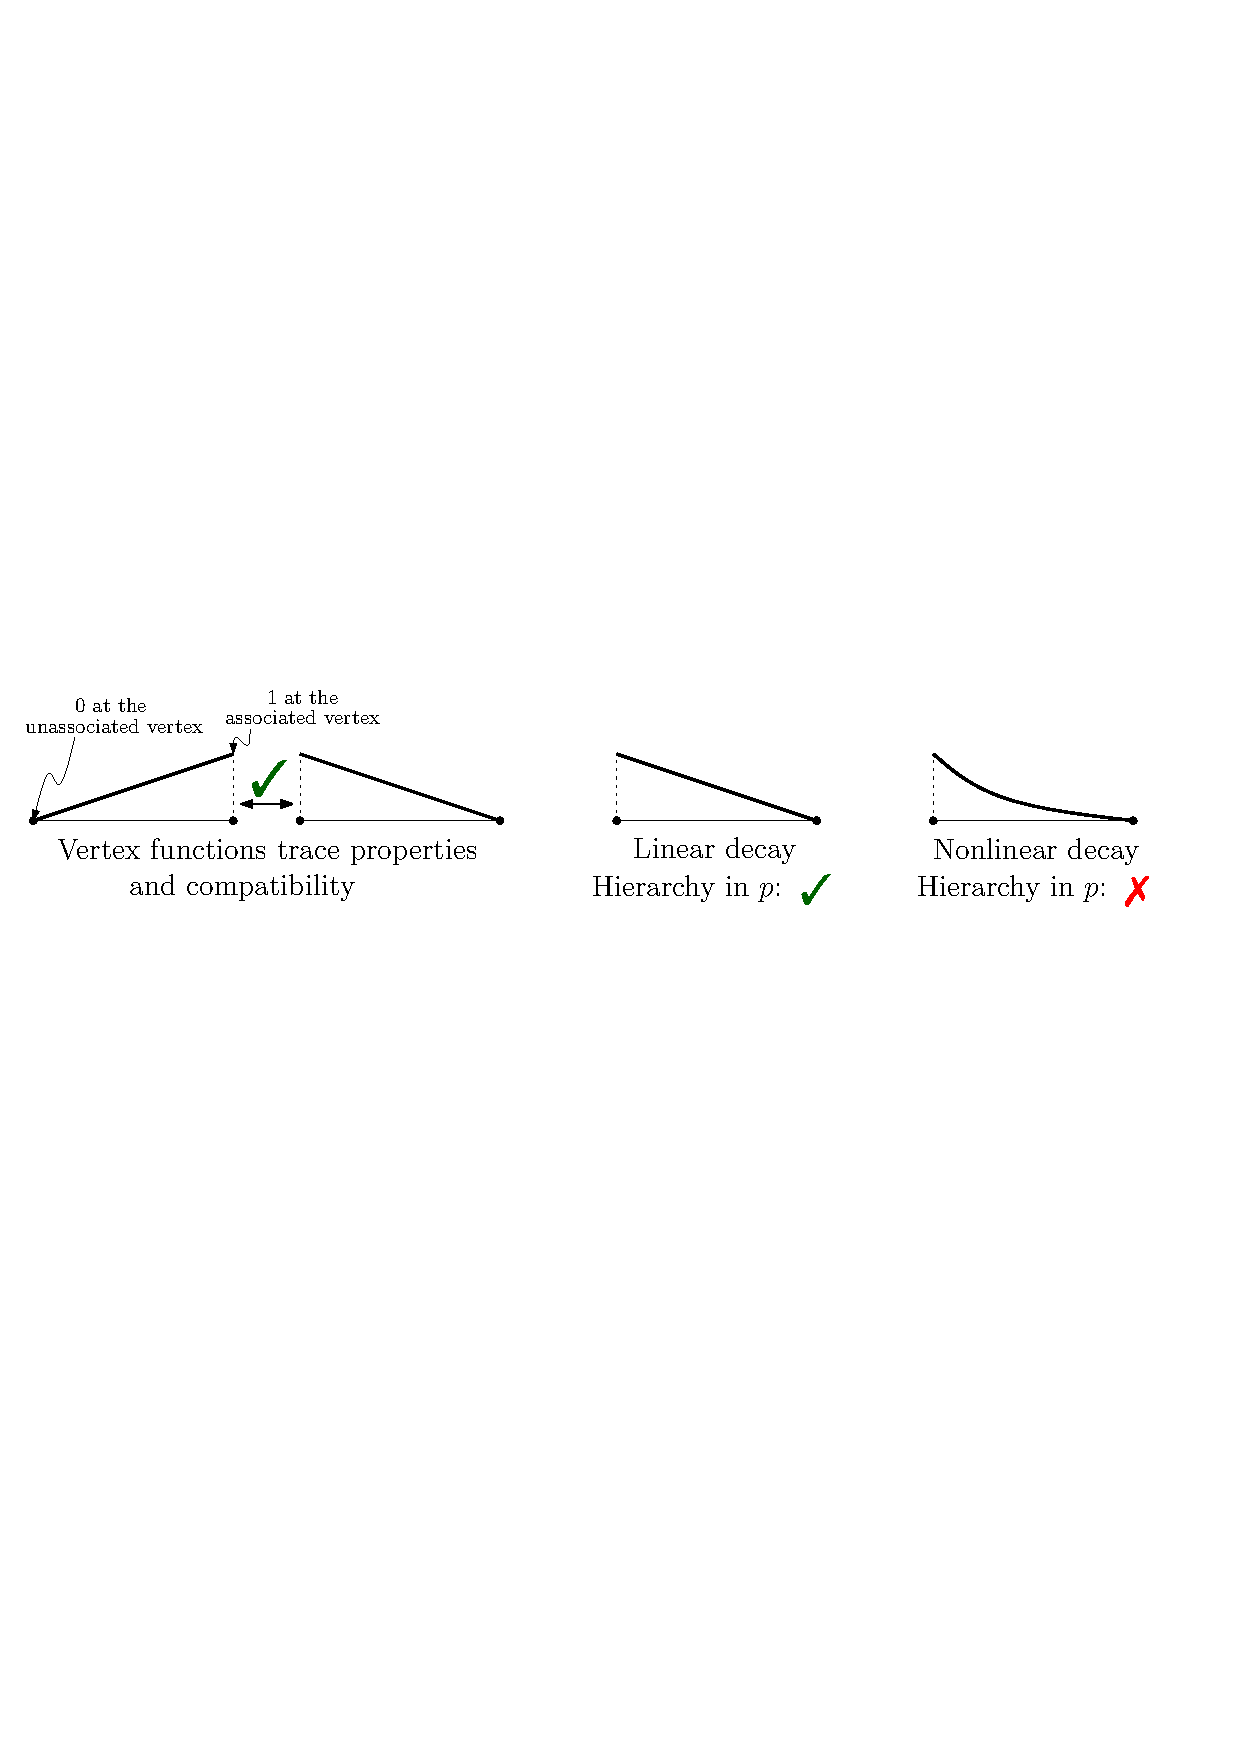
\includegraphics[scale=0.7]{./figures/VertexCompatibilityAndBlending.pdf}
\caption{Natural vertex function compatibility and the different possible decays.}
\label{fig:vertexcompatibility}
\end{center}
\end{figure}

%In general, functions which vanish at \textit{all} of the boundary are called \textit{bubbles}.
\textit{Edge functions:} In 1D the $H^1$ edge shape functions are called \textit{edge bubbles} and should vanish at the two endpoints of the edge (or segment).
This makes them automatically compatible in 1D.
When $p=1$ there are no edge bubbles, when $p=2$ there is one $p=2$ edge bubble, when $p=3$ there is the $p=2$ bubble and an extra $p=3$ bubble giving a total of two bubbles, and so on.
This results in a hierarchical construction of the shape functions in $p$.
%These hierarchically constructed edge bubbles will constitute the group of edge shape functions.
%They are referred to as \textit{the} 1D $H^1$ edge bubbles.

%Due to the dimensional hierarchy, the 1D trace of $H^1$ vertex and edge functions of elements in higher dimensions (quadrilateral, triangle, hexahedron, etc.) will be precisely the 1D $H^1$ vertex and edge functions.
%This is important, because as evidenced by \eqref{eq:traceexactsequences}, the trace of $H^1$ edge functions of elements in higher dimensions (quadrilateral, triangle, hexahedron, etc.) will be exactly one of \textit{the} 1D $H^1$ edge bubbles (modulo an orientation).

\begin{figure}[!ht]
\begin{center}
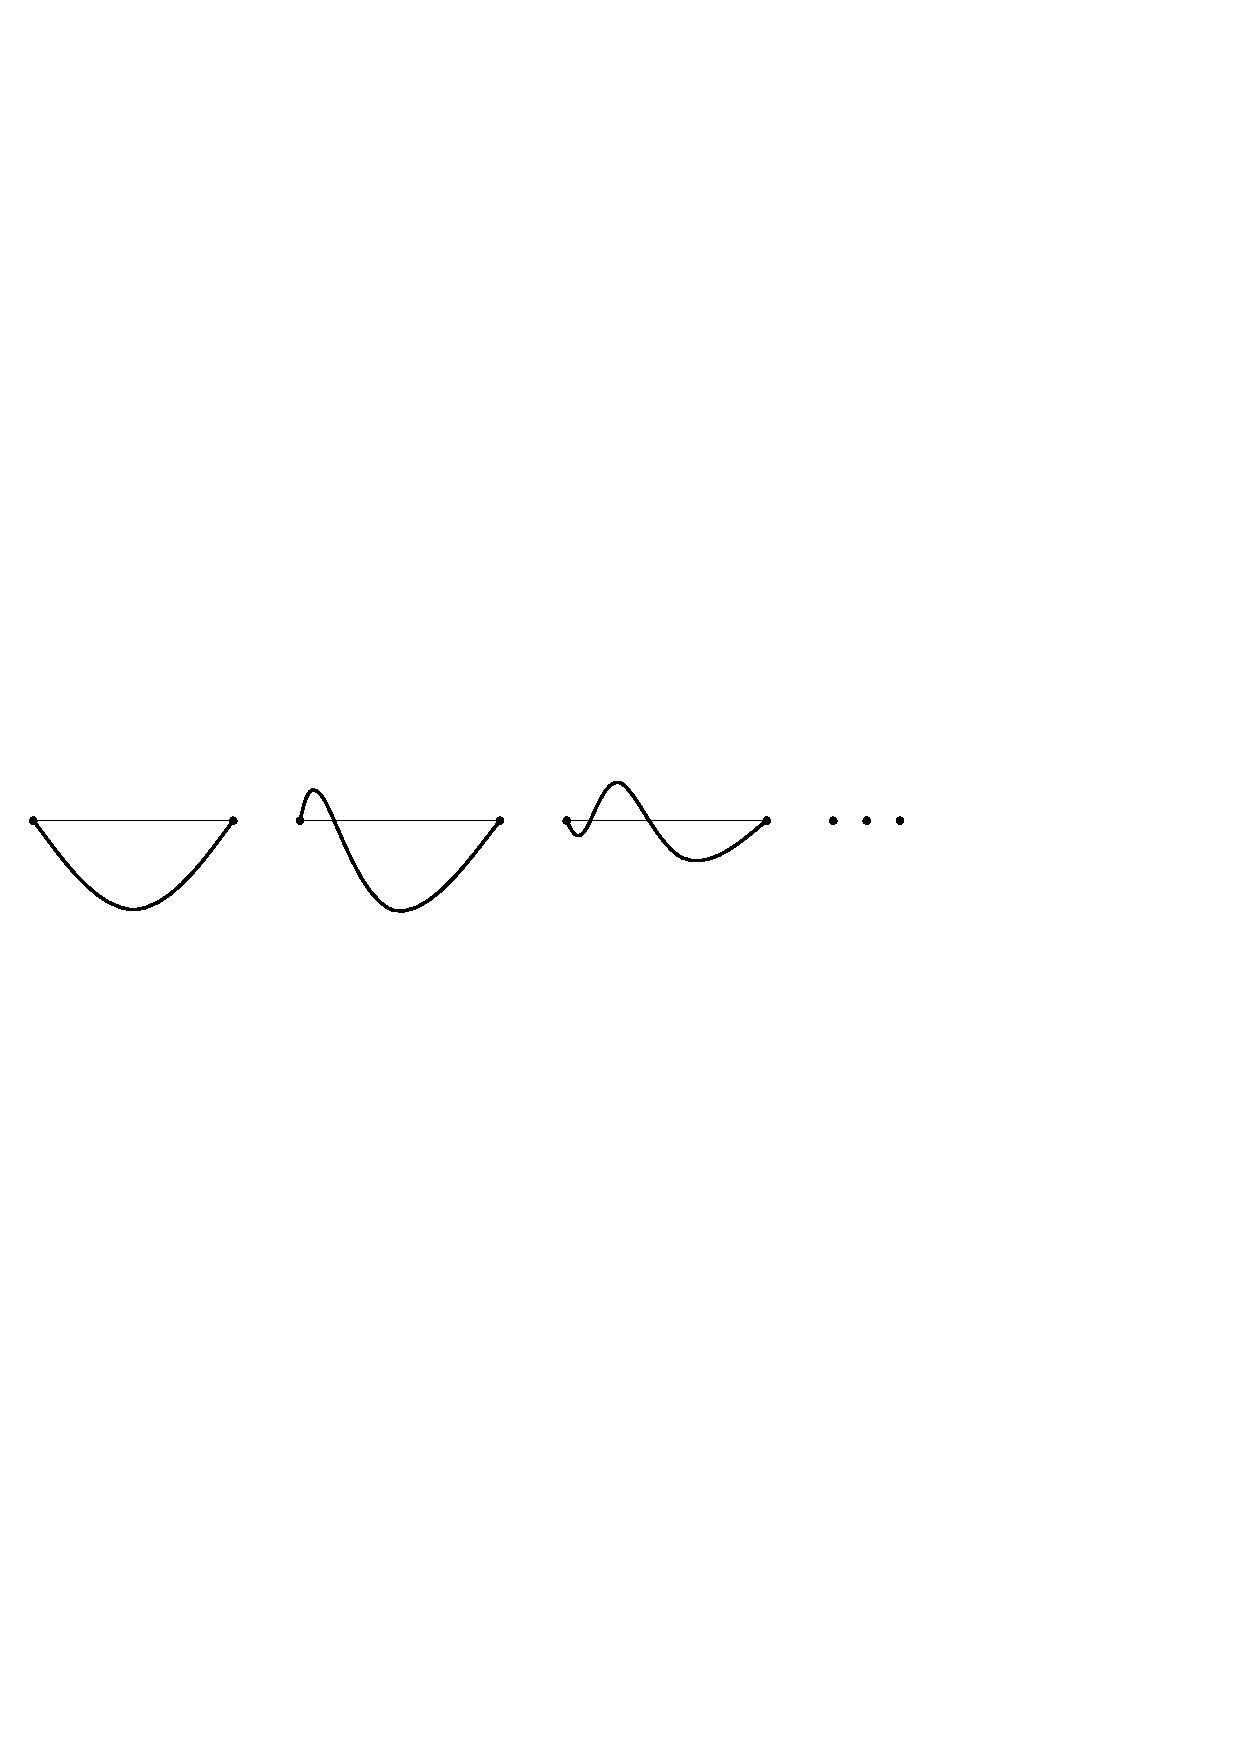
\includegraphics[scale=0.7]{./figures/H1Bubbles.pdf}
\caption{Potential set of of 1D $H^1$ edge bubbles vanishing at both endpoints.}
\label{fig:1DH1bubbles}
\end{center}
\end{figure}

\paragraph{$L^2$.}
\textit{Edge functions:}
The 1D $L^2$ edge functions do not need to satisfy any trace properties (neither vanishing nor nonzero) because there is no notion of trace.
They span the space of the (1D) gradients of the $H^1$ conforming shape functions, and should be hierarchical in their construction.
%They are referred to as \textit{the} 1D $L^2$ edge functions.

\subsubsection{2D}

In two dimensions, classification of shape functions is:
\begin{align*}
  	H^1:&\quad\text{vertex, edge, and face functions,}\\
  	H(\mathrm{curl}):&\quad\text{\phantom{vertex,} edge, and face functions,}\\
  	L^2:&\quad\text{\phantom{vertex, edge, and} face functions.}
\end{align*}
There are two 2D elements: the quadrilateral and the triangle.
Their boundaries are composed of edges and vertices.
%For a given element, each vertex is related to \textit{one} vertex shape function, each edge is associated to a set of edge funtions, and the face is associated to a set of face functions.
%The edge is associated to a set of edge functions.

\paragraph{$H^1$.}
\textit{Vertex functions:}
The vertex functions should vanish at the other (unassociated) vertices and disjoint edges.
They should take the value $1$ at the associated vertex.
In 2D, at this point, this does \textit{not} guarantee compatibility.
However, dimensional hierarchy requires the (nonzero) trace of vertex functions over the adjacent edges to be precisely a 1D $H^1$ vertex function (associated to the vertex in question).
This results in full compatibility, and implies the 2D vertex functions are extensions of their 1D analogues.
%Here, one additionally has to ensure that the trace  always presents the same decay.
%For example, see Figure \ref{fig:2Dvertexcompatibility} (right) for a pair of vertex shape functions satisfying the correct vanishing properties, but being incompatible due to the different decay across the edges.
%If dimensional hierarchy is used, the form of this decay is fixed, since it should
%In this case, compatibility across the boundary would be automatically satisfied (see left of Figure \ref{fig:2Dvertexcompatibility}).
%Fortunately, the
%This is the choice in our work.
%Third, there is the form of the vertex functions themselves along the 2D face (quadrilateral or triangle).
Regarding the form of the shape functions across the (quadrilateral or triangle) face itself, they can have different forms of decay.
Again, hierarchy in $p$ will restrict our choice, so that the vertex functions we define lie in the lowest order space possible.
Indeed, quadrilateral vertex functions present a bilinear decay, while the decay is linear for triangles.
% This form will be quite restrictive in o
%Otherwise, to satisfy compatibility, one would have to ensure that the trace of vertex functions (for both quadrilateral and triangle) over the edges always presents the same decay.
%To ensure compatibility across edges, it is required that the trace of the vertex functions over the (adjacent) edges presents the same decay regardless of the element type (quadrilateral or triangle).
%This is automatically ensured as long as the nonzero (1D) trace of these functions along each edge is a 1D $H^1$ vertex function.
%That is, the \textit{vertex blending across the edge} should be the same for all edges of the quadrilateral and triangle.
%Notice, there is a (partly induced) \textit{vertex blending across the quadrilateral $($or triangular$)$ face}.
%Again, this choice is restricted by the hierarchy, so in this work it is chosen as bilinear for quadrilaterals and linear for triangles.
%which at this point does not affect compatibility, but it will in three dimensions.
%Again, in this work this blending will be provided by a linear function.

\begin{figure}[!ht]
\begin{center}
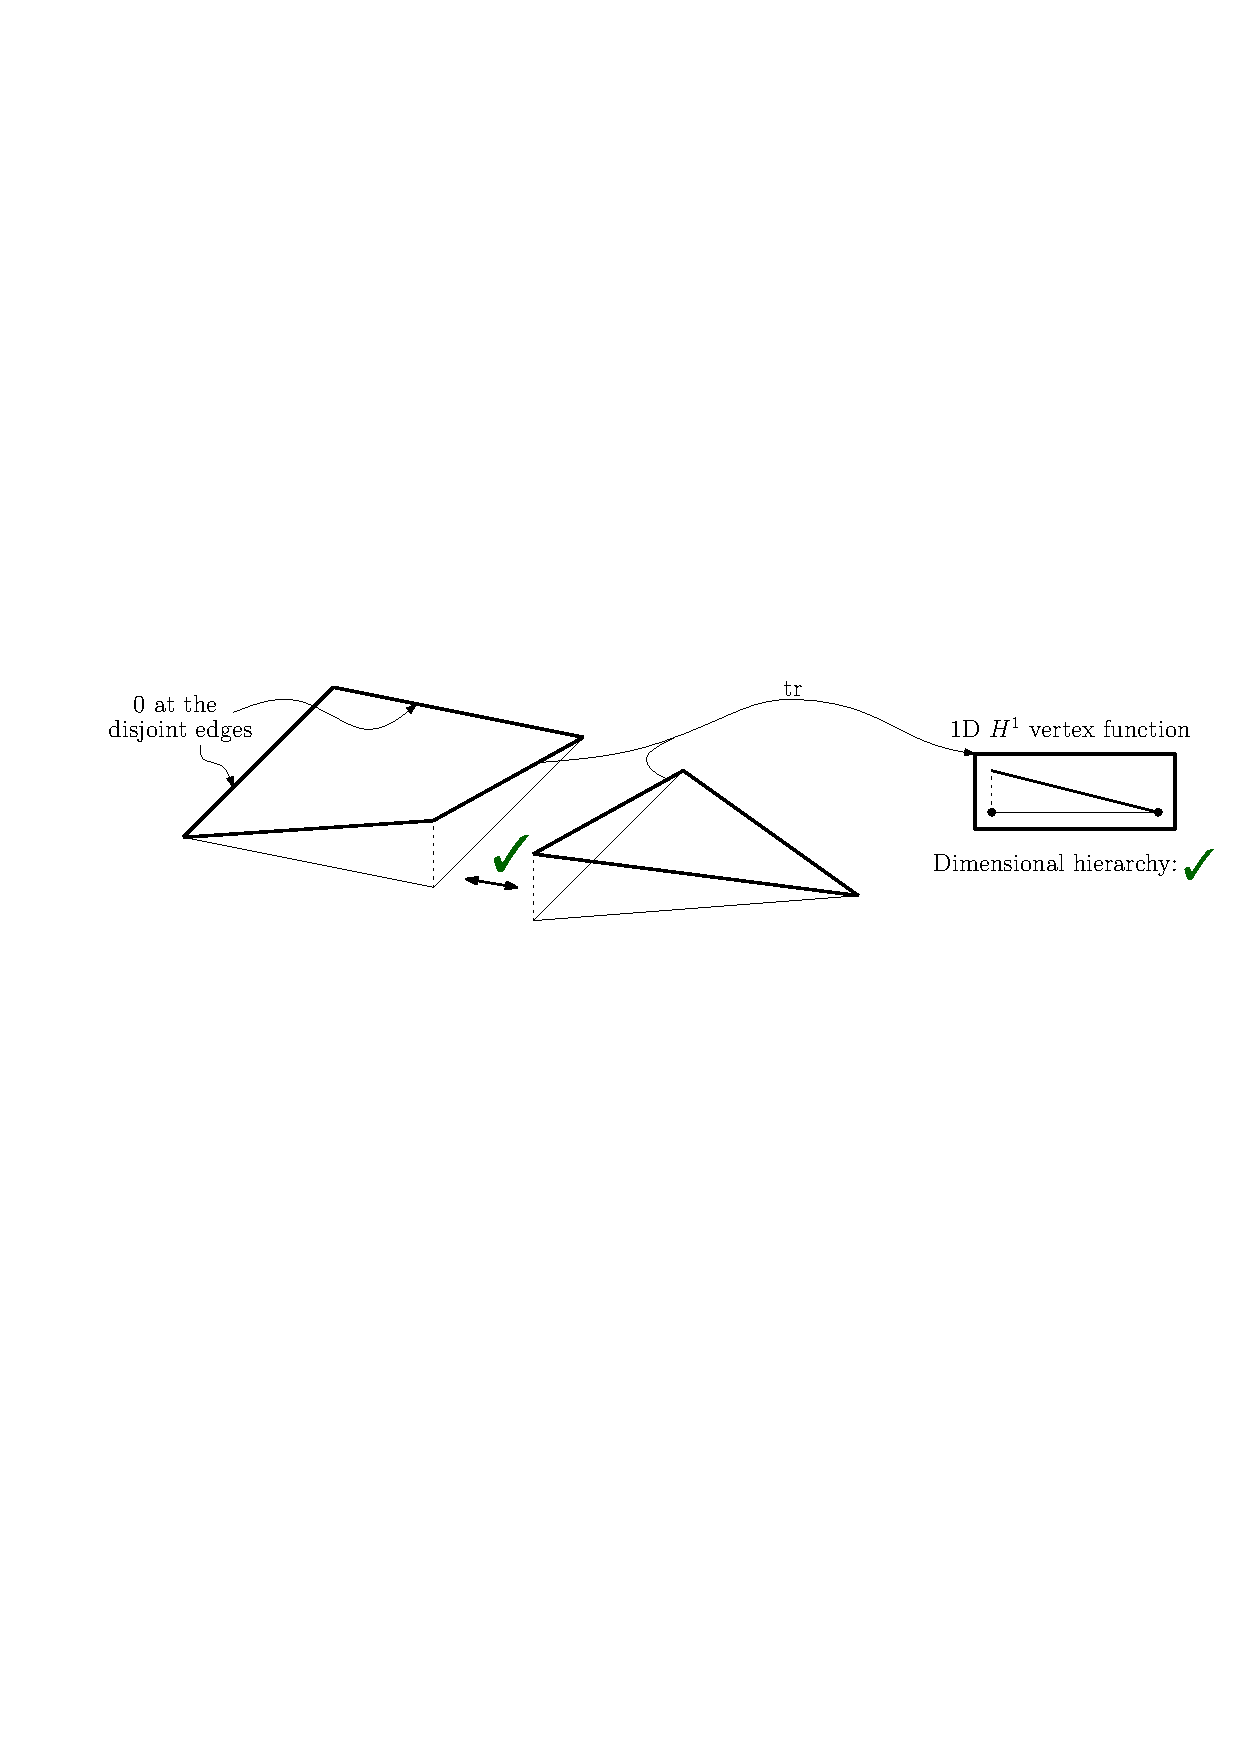
\includegraphics[scale=0.7]{./figures/2DVertexFunctions.pdf}
\caption{Trace properties of 2D $H^1$ vertex functions. Dimensional hierarchy implies full compatibility.}
\label{fig:2Dvertexcompatibility}
\end{center}
\end{figure}

\textit{Edge functions:}
Edge functions should vanish at all other (unassociated) edges of the element.
By dimensional hierarchy, for a given order $p$, the nonzero trace over the (associated) edge itself should take the form of a 1D $H^1$ edge bubble of order $p$.
This gives compatibility modulo edge ``orientations'' in 2D, and it implies the edge functions are extensions of the original 1D $H^1$ edge bubbles.
%All edge shape functions (of a given order $p$) should present the same nonzero trace over the (associated) edge itself.
%Indeed, by \eqref{eq:traceexactsequences} and by dimensional hierarchy, if the trace of the edge functions are the 1D $H^1$ edge bubbles, then compatibility modulo ``orientations'' is satisfied.
%In view of the embeddings shown in \eqref{eq:traceexactsequences}, it follows that at the edge itself the function is one of \textit{the} 1D $H^1$ edge bubbles (the ones coming from the 1D element).
%This is enough to ensure compatibility (modulo orientations) across the boundaries.
%This would imply the edge functions are extensions of the original 1D $H^1$ edge bubbles.
%The extension to the rest of the element involves satisfying the vanishing properties at the other edges, meaning that the function has to somehow decay.
Now, the functions themselves should present a certain decay from the (associated) edge towards the rest of the element.
%This decay is referred to as \textit{edge blending across the quadrilateral $($or triangular$)$ face}.
Again, this choice is generally restricted by the hierarchy in $p$.
For the quadrilateral element the decay we invoke is linear, but things are more complicated for the triangle element. %where the order of decay depends upon the order of the edge function.
%This affects compatibility of the edge functions only in 3D.

\begin{figure}[!ht]
\begin{center}
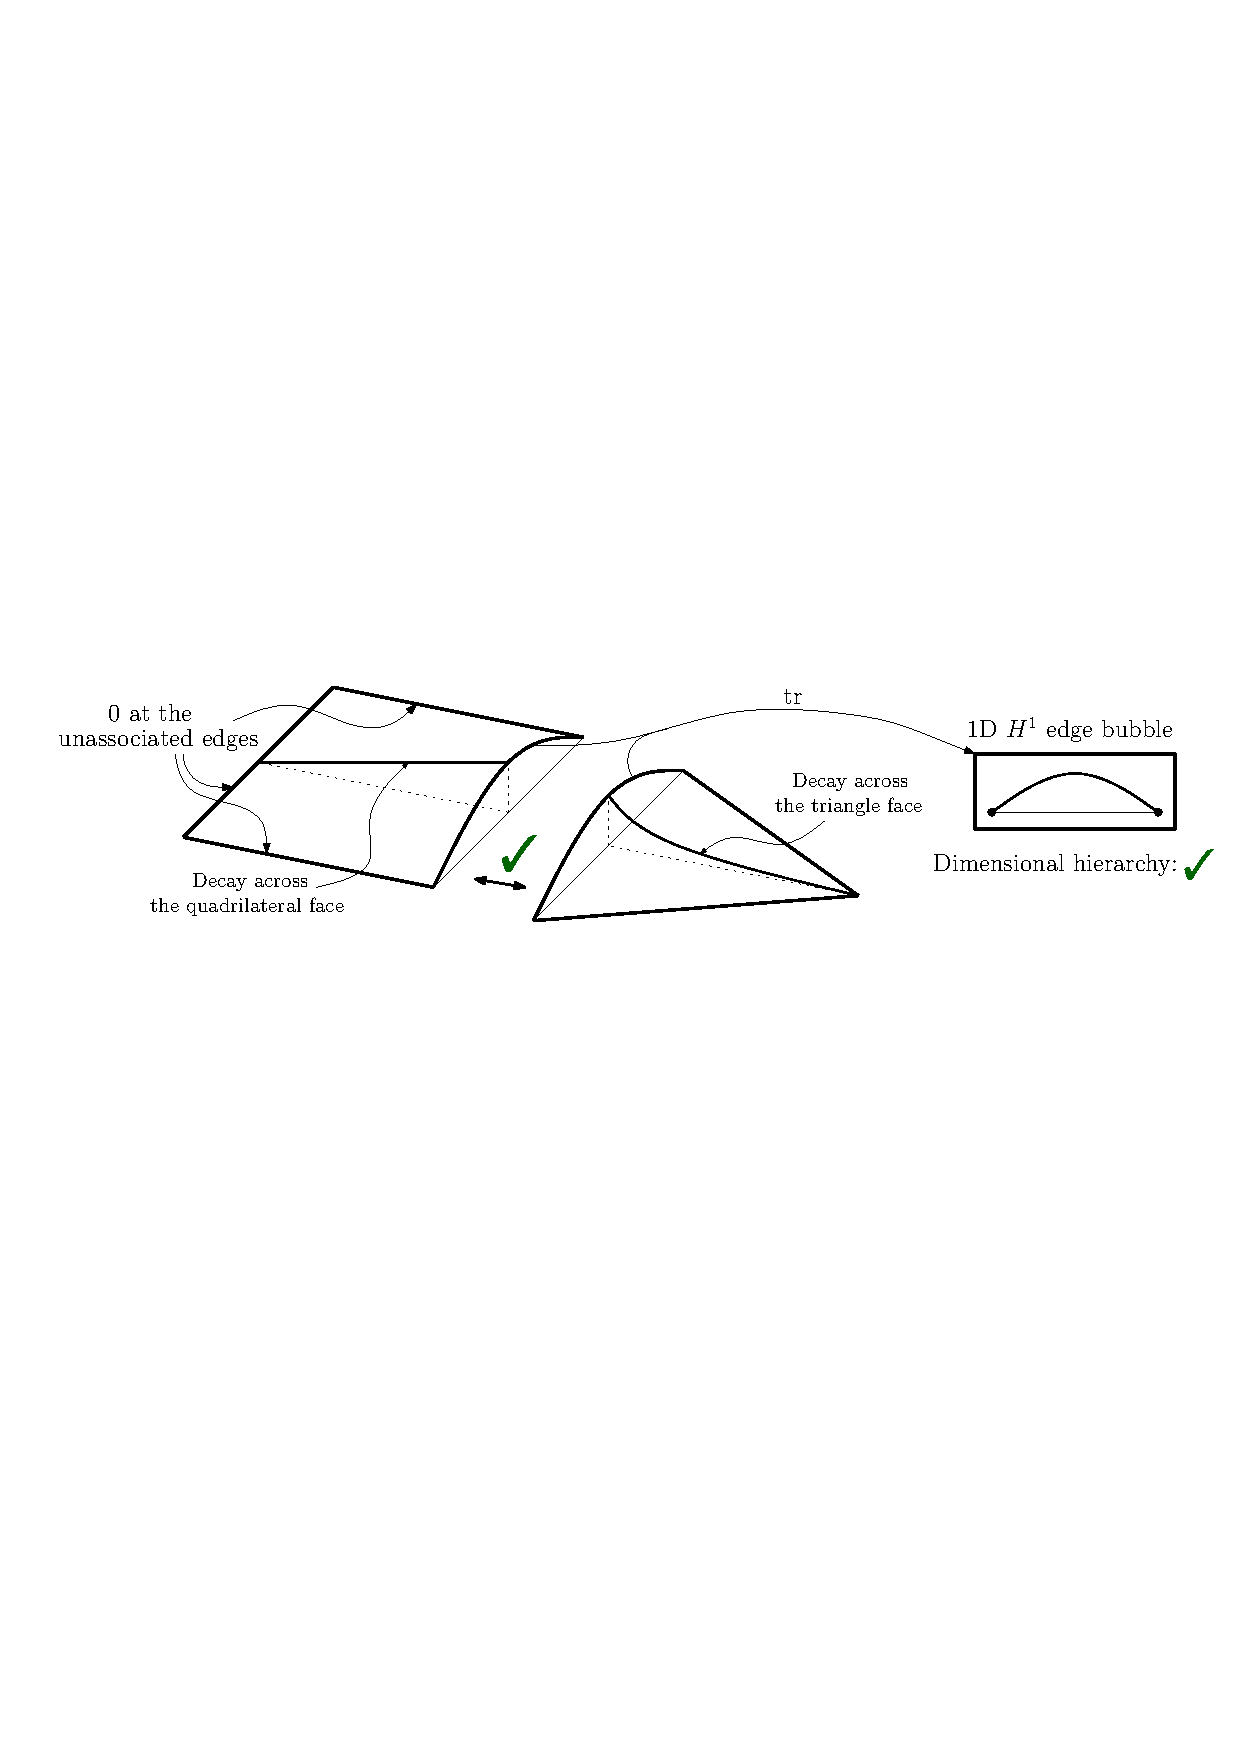
\includegraphics[scale=0.7]{./figures/EdgeBlendingQuadTri.pdf}
\caption{Compatibility of edge functions. Depicted as well is the decay across the faces.}
\label{fig:2Dedgecompatibility}
\end{center}
\end{figure}

\textit{Face functions:}
The 2D \textit{face bubbles} vanish at all the edges of the element, so they are automatically compatible in 2D.
They are constructed usually by using the edge functions previously defined (since these already satisfy some vanishing properties) and making some modifications to establish the remaining vanishing conditions.
Again, their construction is hierarchical in $p$.
%The resulting functions are said to be \textit{the} 2D $H^1$ quadrilateral (or triangle) face bubbles.

\paragraph{$H(\mathrm{curl})$.}
\textit{Edge functions:}
The edge functions must have vanishing (tangential) trace at all other edges.
For a given order $p$, the nonzero (tangential) trace over the edge itself should take the form of a 1D $L^2$ edge function of order $p$.
This ensures compatibility modulo edge ``orientations''.
%Meanwhile, the (tangential) trace of the edge functions (of order $p$) over the edge itself (which has one component) should be the same.
%By dimensional hierarchy (see \eqref{eq:traceexactsequences}), if they are chosen as the 1D $L^2$ edge functions, full compatibility is ensured.
Now, to respect hierarchy in $p$, the edge functions themselves should present a decay (in each of their two components) which is consistent with the lowest order possible decay.
Ultimately, the decay will be similar to that of $H^1$ edge functions.

\textit{Face functions:}
The face bubbles have zero (tangential) trace over all edges, so they are automatically compatible.
They are hierarchically constructed using the same ideas as for their $H^1$ counterparts.
%They are said to be \textit{the} 2D $H(\mathrm{curl})$ quadrilateral (or triangle) face bubbles.

\paragraph{$L^2$.}
\textit{Face functions:}
The $L^2$ face functions do not need to satisfy any trace properties, because there is no notion of trace in $L^2$.
They span the space of (2D) curls of the $H(\mathrm{curl})$ shape functions, and their construction should be hierarchical in $p$.
%and are said to be \textit{the} 2D $L^2$ quadrilateral (or triangle) face functions.

\subsubsection{3D}

In three dimensions, classification of shape functions is:
\begin{align*}
  H^1:&\quad\text{vertex, edge, face, and interior shape functions,}\\
  H(\mathrm{curl}):&\quad \text{\phantom{vertex,} edge, face, and interior shape functions,}\\
  H(\mathrm{div}): &\quad\text{\phantom{vertex, edge,} face, and interior shape functions,}\\
  L^2:&\quad\text{\phantom{vertex, edge, face, and} interior shape functions.}
\end{align*}
There are four 3D elements: the hexahedron, the tetrahedron, the prism and the pyramid.
Their boundaries are composed of faces, edges, and vertices.
%For a given element, each vertex is related to \textit{one} vertex shape function, each edge is associated to a set of edge funtions, each face is associated to a set of face functions, and the interior is associated to a set of interior functions.


\paragraph{$H^1$.}
\textit{Vertex functions:}
Vertex functions have to vanish at all other (unassociated) vertices and at all disjoint edges and faces.
Dimensional hierarchy requires the (nonzero) trace of vertex functions over the adjacent faces to be precisely a 2D $H^1$ vertex function (associated to the vertex in question).
This ensures full compatibility of the vertex functions in 3D.
%The decay of the functions across edges \textit{and} faces should be the same in order to enforce compatibility.
%Hence, the vertex functions of all elements should present the same nonzero vertex blending across the edges.
%The same goes for the vertex blending across quadrilateral and triangular faces.

\textit{Edge functions:}
Edge shape functions should vanish at all other (unassociated) edges and disjoint faces.
By dimensional hierarchy, for a given order $p$, the nonzero trace over the adjacent faces should be a 2D $H^1$ edge function of order $p$ (associated to the edge in question).
Again, this ensures compatibility modulo edge ``orientations''.
%Again, the trace of functions at the edge itself must be one of \textit{the} 1D $H^1$ edge bubbles, so they are 3D extensions of the original 1D function.
%To ensure compatibility (modulo orientations), the functions should have the same \textit{edge} blending across the quadrilateral faces and the triangular faces.

\textit{Face functions:}
Face functions should vanish at all other (unassociated) faces.
Dimensional hierarchy establishes that, for a given order, the nonzero trace over the (associated) face itself should be a 2D $H^1$ face bubble of the same order.
This establishes compatibility modulo face ``orientations''.

\textit{Interior functions:}
The 3D \textit{interior bubbles} vanish at all faces of the element, and are fully compatible in 3D.
Our construction of these functions usually involves making some changes to the face functions previously defined in order to establish the remaining vanishing conditions.

\paragraph{$H(\mathrm{curl})$.}
\textit{Edge functions:}
The edge functions must have vanishing (tangential) trace at all other edges and disjoint faces.
For a given order $p$, the nonzero trace over the adjacent faces should be a 2D $H(\mathrm{curl})$ edge function of order $p$.
This gives compatibility modulo edge ``orientations''.
%As mentioned before the (tangential) trace of the edge function over the edge itself (which has one component) must be one of \textit{the} 1D $L^2$ edge functions.
%For compatibility, the \textit{edge} blending across the quadrilateral faces and the triangular faces should be the same.

\textit{Face functions:}
The face functions have vanishing (tangential) trace over all other faces.
%Using \eqref{eq:traceexactsequences} it is clear that the (tangential) trace over the face must be one of \textit{the} 2D $H(\mathrm{curl})$ quadrilateral or triangle face bubbles.
Requiring the trace over the face itself to be a 2D $H(\mathrm{curl})$ face bubble of a given order ensures compatibility modulo face ``orientations''.

\textit{Interior functions:}
The interior bubbles have zero (tangential) trace over all the faces and are fully compatible in 3D.
They are constructed using the same ideas as for interior bubbles in $H^1$.

\paragraph{$H(\mathrm{div})$.}
%In this space, there are no vertex or edge functions.
\textit{Face functions:}
The face functions should have vanishing (normal) trace at all other faces.
The trace over the face itself should be a 2D $L^2$ face function of a given order.
%Due to \eqref{eq:traceexactsequences}, they will be extensions of 2D $L^2$ face functions, and their normal component along the face should be one of \textit{the} 2D $L^2$ quadrilateral or triangle face functions.
Compatibility modulo face ``orientations'' is then established.

\textit{Interior functions:}
The interior bubbles have zero normal component at all the faces, and they are automatically compatible.
They are constructed using the same ideas as in $H^1$.

\paragraph{$L^2$.}
\textit{Interior functions:}
These do not have to satisfy any trace properties and they span the space of the (3D) divergences of the $H(\mathrm{div})$ shape functions.

% We shall always identify the discrete spaces first, and only then introduce the corresponding shape functions that provide bases for those spaces. It is in place perhaps to recall two competing schools of thought when it comes to the concept of shape functions.

% The classical definition of Ciarlet \cite{Ciarlet} starts with {\em degrees-of-freedom} that are functionals defined on a larger space $\mathcal{X}(\Omega)$ that contains both the space of element shape functions
% $X(\Omega)$  and the exact solution,
% $$
% \psi_j : \mathcal{X}(\Omega) \to \mathbb{R}, \quad j=1,\ldots, N_\Omega \, .
% $$
% Here, $N_\Omega$ denotes the number of degrees of freedom. In this definition,the condition of {\em unisolvability} is critical; the restrictions, $\psi_j\vert_{X(\Omega)}$, must provide a basis for the algebraic dual space $X(\Omega)^\ast$. The element shape functions $\phi_i$ are defined then as the {\em dual basis} to the degrees-of-freedom,
% $$
% \psi_j(\phi_i) = \delta_{ij},\quad i,j=1,\ldots,N_\Omega \, .
% $$
% This naturally leads to the definition of the {\em interpolation operator}:
% $$
% \Pi : \mathcal{X}(\Omega) \ni u \to \Pi u := \sum_{j=1}^{N_\Omega} \psi_j(u) \phi_j \in X(\Omega) \,  .
% $$
% A judicious choice of degrees-of-freedom must guarantee {\em global conformity}, i.e. by ``gluing'' (taking unions of) shape functions, global Galerkin {\em basis functions} are constructed which belong to the appropriate energy spaces. Global conformity depends  upon the energy space. For instance, $H^1$-conforming shape functions must be globally continuous while the vector-valued $H(\text{curl})$-conforming shape functions must only be continuous in their tangential components across interelement boundaries. Similarly, for vector-valued $H(\text{div})$-conforming shape functions, only the continuity of only the normal component is enforced. Finally, $L^2$-conformity does not involve any continuity assumptions at all.

% Different energy spaces also lead to different notion of {\em traces}. By the $H^1$ trace of a scalar-valued (sufficiently) regular function, we understand simply its restriction to the boundary. By the (tangential) $H(\text{curl})$ trace of a vector-valued function, we understand the restriction of its {\em tangential component} on the boundary. Thus, the  $H(\text{curl})$ trace of a two component function $(E_1,E_2)$ in $\mathbb{R}^2$ to an element edge, is going to be a scalar-valued function. In 3D, however, the trace of a 3D vector-valued function to an element face, will be a 2D vector. Similarly, the (normal) $H(\text{div})$ trace of a vector-valued function to an edge (2D) or a face (3D) is always a vector orthogonal to the element boundary that involves
% just one scalar component.

% Global conformity considerations lead naturally to the classification of degrees-of-freedom and also naturally distributes the shape functions into groups related to geometric entities:
% $$
% \begin{array}{rl}
%   H^1:& \text{vertex, edge, face, and interior shape functions,}\\
%   H(\text{curl}):& \text{\phantom{vertex,} edge, face, and interior shape functions,}\\
%   H(\text{div}): & \text{\phantom{vertex, edge,} face, and interior shape functions,}\\
%   L^2:  & \text{\phantom{vertex, edge, face, and} interior shape functions.}
% \end{array}
% $$
% When following the Ciarlet construction, we must precompute the shape functions in terms of (usually) combinations of monomials and store the corresponding coefficients.


% The competing approach of Szabo \cite{SzaboBabuska91} starts with a direct construction of shape functions by following the geometric classification above. The shape functions are defined in terms of Legendre and Jacobi polynomials and their integrals, and are computed using simple recursive formulas. This is the approach taken in this work. Note that, in Szabo's approach, we do not define the interpolation operators at this point at all. The so-called {\em projection-based interpolation} \cite{hpbook,hpbook2} defined through local projections over element edges, faces and interior, is introduced {\em independently} of the construction of shape functions. With no need to precompute coefficients defining  the shape functions, following Szabo's approach is perhaps more convenient.

%The geometric definition of shape functions implies the corresponding {\em vanishing properties}. For instance, an $H^1$ vertex shape function corresponding to a particular vertex is unity at that vertex and vanishes at all remaining vertices. An edge shape function will be non-zero along a particular edge but it will vanish along all remaining edges. A similar property holds for the face shape functions. The trace of interior shape functions ({\em element bubbles}) will vanish on the entire element boundary and so the corresponding basis functions will be supported over the element only. Debugging of shape function routines starts usually with verification of the appropriate vanishing properties.

%\subsection{Complying with the exact sequence structure}
%\label{sec:exactsequenceembeddings}
%Construction of element shape functions should comply with the logic of 1D and 2D exact sequences for traces of element shape functions to edges and faces \cite{Schoeberl_Zaglmayr_05}. This is to a certain extent satisfied automatically in our constructions as {\em we begin} with 1D edge or 2D face shape functions defined on edges or faces and only later extend them to the element. The extensions comply with the logic of exact sequences in the sense that the ultimate 3D edge or face functions utilize only the information provided by the 1D edge or 2D face routines. For instance, construction of $H(\text{curl})$ shape functions begin with a 1D $L^2$ shape function defined along the edge that constitutes the tangential components (along the edge) of the corresponding 2D or 3D shape function. The 1D $L^2$ shape functions come with no derivative. Consequently, the computation of the curl of 2D or 3D extension must not involve such a derivative either. In the same way, an $H(\text{curl})$ face shape function should use only the tangential trace and its surface curl on the corresponding face, and the $H(\text{div})$ shape functions should use only the values of their normal components on the face.
%
%We illustrate this affinity to the exact sequence at the trace level with the following diagram applying to a 3D element:
%\begin{displaymath}
%  %\text{2D:}&\qquad H^1 \xrightarrow{\,\,\nabla\,\,} H(\mathrm{curl}) \xrightarrow{\nabla\times} L^2 \\
%  %\text{1D:}&\qquad H^1 \xrightarrow{\,\,\nabla\,\,} L^2\,.
%  \xymatrix{
%        {\text{Interior:}} & H^1 \ar[r]^{\nabla\,\,\,\,} \ar@{.>}[d]^{\mathrm{tr}} & H(\mathrm{curl})
%          \ar[r]^{\,\,\,\nabla\times} \ar@{.>}[d]^{\mathrm{tr}} & H(\mathrm{div}) \ar[r]^{\,\,\,\nabla\cdot} \ar@{.>}[d]^{\mathrm{tr}} & L^2\\
%        {\text{Face:}} & H^1 \ar[r]^{\nabla\,\,\,} \ar@{.>}[d]^{\mathrm{tr}} & H(\mathrm{curl})
%          \ar[r]^{\,\,\,\nabla\times} \ar@{.>}[d]^{\mathrm{tr}} & L^2\\
%        {\text{Edge:}} & H^1 \ar[r]^{\nabla\,\,\,\,} & \,\,\,\,L^2\,\, }\,.
%\end{displaymath}
%Here, the ``mapping arrows,'' $\xymatrix{{}\ar@{.>}[r]^{\mathrm{tr}}&{}},$ indicate that the range is actually a larger space. These arrows are meant to be motivational only.
%% For example, this suggests that the traces of discrete $H(\mathrm{div})$ functions should be in a two dimensional $L^2$ space.
%% For the polynomial spaces, this means the face functions should involve traces which are products of Legendre polynomials $P_i$.
%% Moreover, they should go in the normal component to the face.
%At the discrete level, we reproduce the above diagram precisely with the dotted lines being replaced by well-defined maps. One benefit in this approach is that it allows for a large degree of portability of code from one element construction to another.
%% Indeed we acheive this.
%
%The second aspect of the exact sequence philosophy is a careful choice of discrete energy spaces. In our discrete exact sequences for the triangle and tetrahedral elements, we use the well known $H(\text{curl})$-conforming \Nedelec~and $H(\text{div})$-conforming Raviart-Thomas spaces.\footnote{See definitions for these spaces in \S~\ref{sec:Tri} and \S~\ref{sec:Tet}.} Unlike other higher order discete energy spaces used in the literature, these spaces happen to be affine invariant while also preserving a commuting exact sequence structure. In fact, we make the distinction that all of our discrete exact sequences preserve a commuting exact sequence stucture which then ensures interpolation estimates for all of our energy spaces. \textit{cite}

\subsection{Orientation Embedded Shape Functions}
\label{sec:introorientations}

\begin{figure}[!ht]
\begin{center}
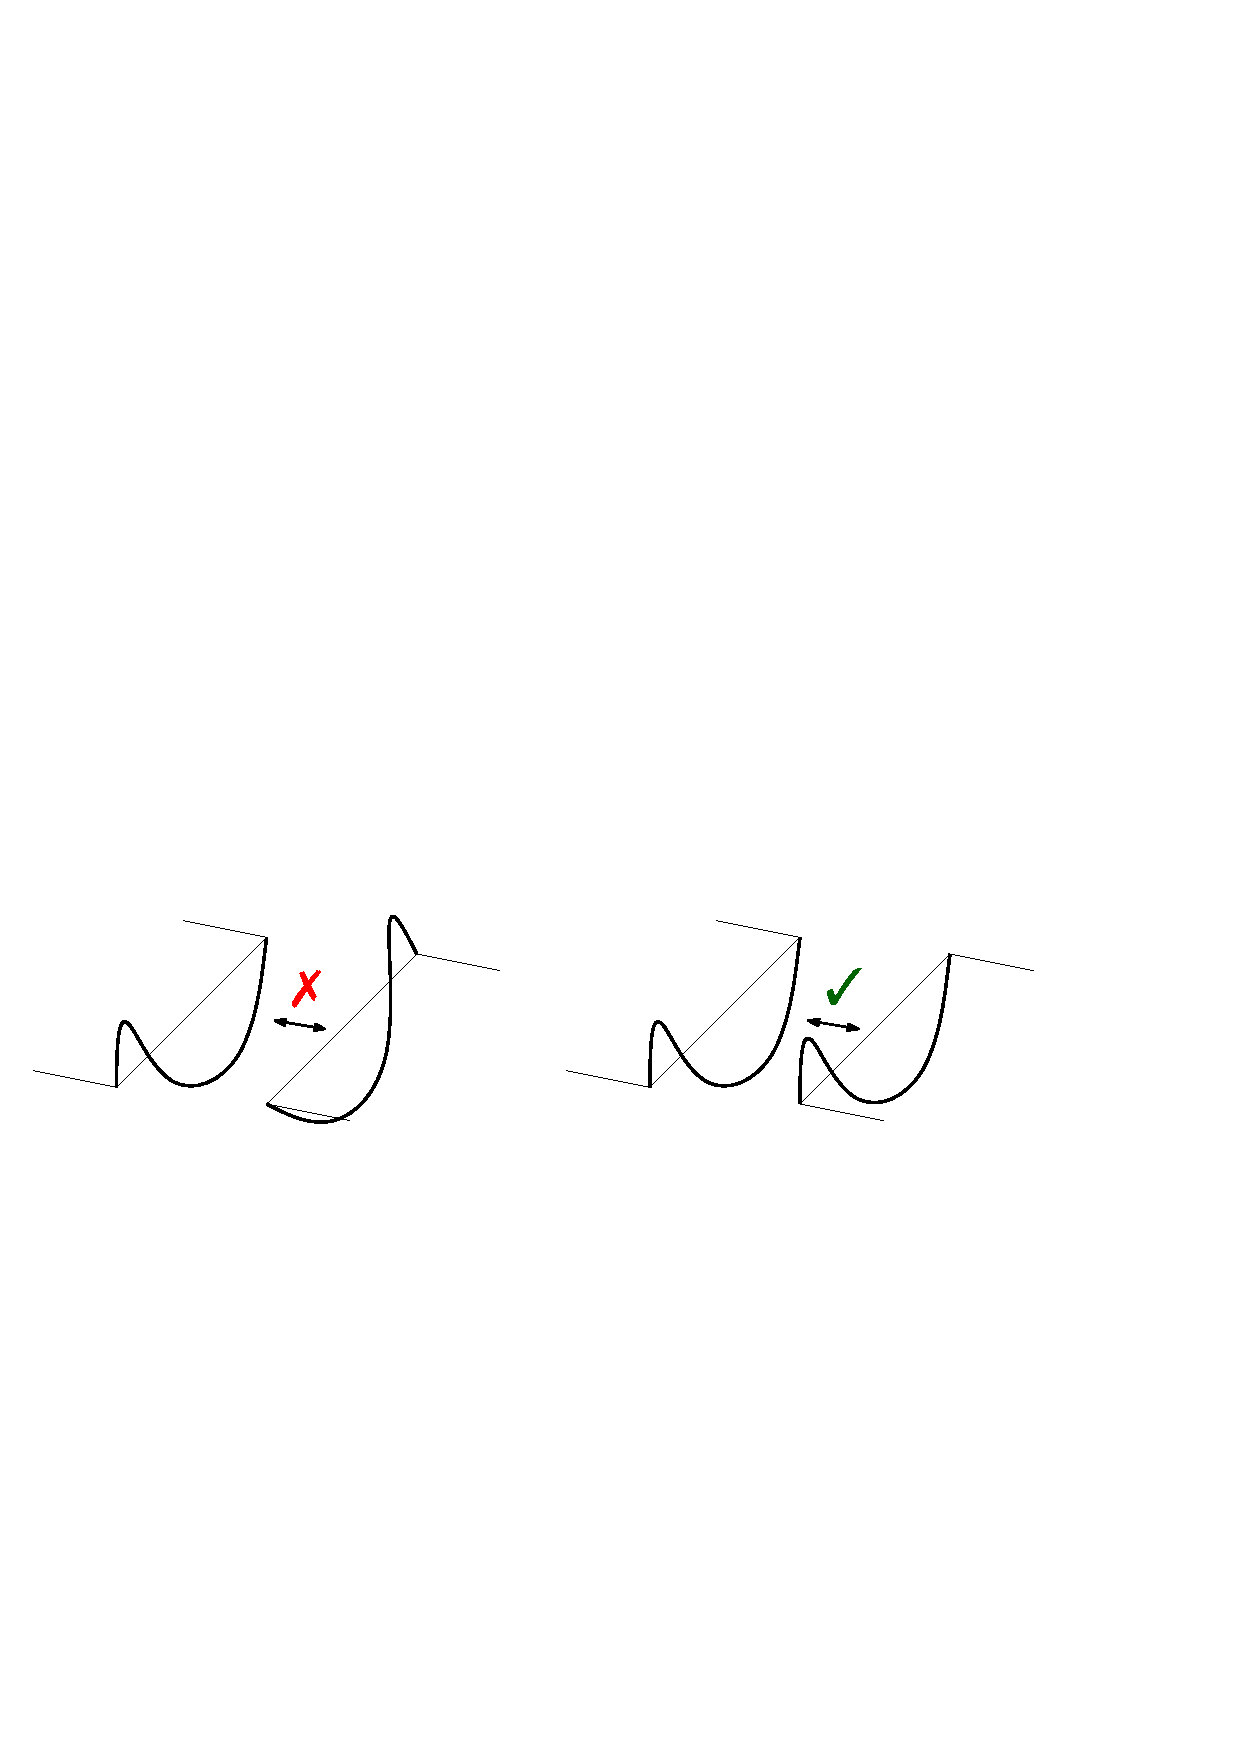
\includegraphics[scale=0.7]{./figures/OrientationsEdgeMismatch.pdf}
\caption{Potential edge function ``orientation'' mismatch in 2D due to disregarding the global mesh.}
\label{fig:edgemismatchintro}
\end{center}
\end{figure}

To ensure \textit{full} compatibility of the shape functions along the boundaries, the concept of \textit{orientations} needs to be introduced.
The simplest example occurs in 2D, where edge functions might not match in the \textit{global} mesh due to a simple change in coordinates over the edge itself.
This ``orientation'' mismatch occurs when the edge functions in the (local) master element are transformed to the global mesh.
Indeed, in the standard Szab\'o's approach, master element shape functions are constructed with no regard for global edge or face coordinates, and element shape functions contributing to an edge or face basis function may not coincide with each other along the shared boundary.
This leads to the necessity of an additional action during the finite element assembly process to account for local-to-global orientation changes (change of coordinates).
Usually, these involve \textit{sign factors} in the case of edges and quadrilateral faces, and more complicated adjustments in the case of triangle faces (see the discussion in \citet[p.50]{hpbook2}).
In the context of $h$ adaptive codes involving hanging nodes, the implementation of these modifications in the assembly procedure can become quite involved, and alternative solutions to this problem are therefore desired.

One such solution involves the concept of orientation embedding \citep{GattoDemkowicz10}.
Here, a given topological entity (an edge in 2D, or a face or edge in 3D), regardless of what elements it is adjacent to, is given a \textit{global orientation} at the mesh level, so that it effectively owns a system of coordinates.
In the mesh, this is equivalent to ordering the vertices in a certain order for that given topological entity.
For instance, for an edge with vertices $a$ and $b$, the vertices can be ordered as $a\to b$ or $b\to a$. 
This choice defines a certain global edge orientation.
This information is then passed to the master element, and the shape functions are defined depending on this new information.
The resulting shape functions are then \textit{automatically} compatible with each other.
Naturally, at the local level, this constitutes an extension to the typical approach by Szab\'o, but at the assembly level, it simplifies the implementation of constrained approximation (hanging nodes) by an order of magnitude.

In view of these observations, in this work we constructed orientation embedded shape functions which take into account the information regarding the ``orientation'' of each relevant topological entity.
For each element, we explain these orientation embeddings only after first presenting a complete construction of the classical (``unoriented'') shape functions.
Hence, the information is conveniently decoupled for ease of consultation.
%It will be clear that this will not involve too much extra work.
%In the text, for each given element, the orientation embeddedings are only explained after first presenting a complete construction of the classical (``unoriented'') shape functions.
% However, the inclusion of this notion is always briefly explained \textit{after} describing the construction of the classical (``unoriented'') shape functions for each given element.
%Therefore, as a first iteration in trying to implement the shape functions (or for those readers only interested in the standard approach) we encourage to skip the latter explanations on orientations.
%\footnote{Additionally, any reader already having a local-to-global assembly process in place can still use the provided FORTRAN90 code simply by choosing the zero orientation case.}

%Each edge and face in the mesh comes with its own system of coordinates, defining the edge or face {\em global orientation}. At the same time, the common edge or face, shared by two or more elements, is equipped with its own {\em local} coordinates (orientation) implied by the element system of coordinates. In the standard Szabo's approach, master element shape functions are constructed with no regard for global edge or face coordinates, and element shape functions contributing to an edge or face basis function may not coincide with each other along the shared geometric entity. This leads to the necessity of an additional modification of those shape functions in the assembly process to account for the local-to-global orientations (change of coordinates). For hexas and prisms this leads to the use of {\em sign factors}, for triangular faces, the proposed solutions are more complicated (see the discussion in \cite{hpbook2}, p.50). The construction of {\em orientation embedded shape functions}, proposed for the $H^1$ elements in \cite{GattoDemkowicz10}, follows a different strategy. When defining an $H^1$ or $H(\text{curl})$ edge shape function, we assume that the function {\em is owned by the edge}, i.e. it has been defined in the edge-owned, global edge coordinate. The task is then only to {\em extend} it into the face and element while also respecting the face and element spaces. As the extension is constructed in element coordinates, one must transition from the edge-owned to the element-local coordinates before the extension can be performed. Consequently, the element shape function routine must receive on input not only master point coordinates and order for element {\em nodes} (edges, faces and interior) but also the so-called nodal {\em orientations} necessary for defining the local-to-global coordinate transformations. In return, shape functions contributing to the same global basis function are {\em automatically} compatible with each other. For regular meshes, the corresponding assembly procedure collapses to the classical one, and the corresponding implementation of constrained approximation (hanging nodes) becomes easier by an order of magnitude. The nodal orientations constitute part of element-to-node connectivity information, and must be provided by the FE code. Of course, with nodal orientations set to zero, the routines return shape functions defined in element coordinates only and could be used by those already having a local-to-global assembly process in place.


% The last aspect of the exact sequence philosophy is invariance when changing element geometries. Either changing the coordinates parameterizing the element or moving the master element to its physical element in a mesh will induce natural maps between energy spaces. These are called pull-back maps (also called Piola transforms), and they are well documented in the literature. For derivations and a detailed discussion, see \cite{hpbook,hpbook2}.
% These are as follows.
% \begin{description}
%   \item[1D pullback:] $x = x(\xi)$.
% \be
% \begin{array}{rl}
% H^1: &  \phi(x) = \hat{\phi}(\xi(x)) \\[8pt]
% L^2: & \psi(x) = \hat{\psi}(\xi(x)) \frac{d\xi}{dx}
% \end{array}
% \ee
%   \item[2D pullbacks:] $x_i = x_i(\xi_j)$.
% \be
% \begin{array}{rl}
% H^1: &  \psi(x_i) = \hat{\psi}(\xi_j(x_i)) \\[8pt]
% H(\text{curl}): & E_k(x_i) = \hat{E}_l(\xi_j(x_i)) \frac{\ptl \xi_l}{\ptl x_k} \\[8pt]
% L^2: & \psi(x_i) = \hat{\psi}(\xi_j(x_i))/J
% \end{array}
% \ee
%   \item[2D pullbacks (rotated exact sequence):] $x_i = x_i(\xi_j)$.
% \be
% \begin{array}{rl}
% H^1: &  \phi(x_i) = \hat{\phi}(\xi_j(x_i)) \\[8pt]
% H(\text{div}): & V_k(x_i) = \frac{\ptl x_k}{\ptl \xi_l}  \hat{V}_l(\xi_j(x_i))/J \\[8pt]
% L^2: & \psi(x_i) = \hat{\psi}(\xi_j(x_i))/J
% \end{array}
% \ee
%   \item[3D pullbacks:] $x_i = x_i(\xi_j)$.
% \be
% \begin{array}{rl}
% H^1: &  \phi(x_i) = \hat{\phi}(\xi_j(x_i)) \\[8pt]
% H(\text{curl}): & E_k(x_i) = \hat{E}_l(\xi_j(x_i)) \frac{\ptl \xi_l}{\ptl x_k} \\[8pt]
% H(\text{div}): & V_k(x_i) = \frac{\ptl x_k}{\ptl \xi_l}  \hat{V}_l(\xi_j(x_i))/J \\[8pt]
% L^2: & \psi(x_i) = \hat{\psi}(\xi_j(x_i))/J
% \end{array}
% \ee
% \end{description}
% Above, functions with hats are assumed to be functions of $\xi_j$, and $J = \text{det} (\ptl x_i/\ptl \xi_j)$ is the Jacobian of the transformation. The main point of the pullbacks is that they transform the exact sequence in $\xi_j$ domain into an exact sequence in $x_i$ domain. For derivations and a detailed discussion, see \cite{hpbook,hpbook2}.

% The only specific place in our exposition where it is necessary to define the pull-back maps will be in \S~\ref{section:Pyramid} on the pyramid element. %pullback maps will be reintroduced in a specific context different from the other elements. This happens to be because the shape functions are constructed across two different isomorphic geometries. For readers not interested in constructing shape functions for this particular element, nothing but a tacit understanding of the pull-back maps listed above will be necessary.
% Otherwise, we only need to consider element-to-element reparameterizations which present themselves as orientation changes. For all of our shape functions, these reorientations are all handled by permutating affine coordinate functions which we now define.

\subsection{Affine Coordinates}
\label{sec:affinecoordinates}

In this work, we chose to exploit simplex (barycentric) \textit{affine coordinates} to formulate all shape function constructions. %\footnote{Affine-related coordinates, in the case of the pyramid element (see \S\ref{sec:Pyramid}).}
%They conveniently act as auxiliary functions when defining the final shape functions in master element coordinates for each element.
It is well known that affine coordinates are useful when constructing shape functions for the triangle and tetrahedron, which are simplices.
However, we note that with the exception of the pyramid, all elements are either a simplex or a Cartesian product of simplices. 
Indeed, we use these coordinates for \textit{all} the elements, including the pyramid, where we define affine-related coordinates to complement the construction.

Using affine coordinates has many desirable advantages.
Firstly, they give a solid geometrical intuition to the shape functions.
Secondly, they allow the expressions for the shape functions to be used in many other master element geometries.
Lastly, they play a vital role in the context of orientation embedded shape functions.
Indeed, orientation changes are handled almost effortlessly by simple permutations in the arguments of a few crucial \textit{ancillary functions} (or \textit{operators}).
The arguments of these functions are precisely affine coordinates (or affine-related), and they are permuted in accordance to a simple auxiliary permutation function.
% can still be used for the edges, and as a result for other elements which
This property might be somewhat intuitive in the case of $H^1$ functions, but what is remarkable is that it also holds for the relevant $H(\mathrm{curl})$ and $H(\mathrm{div})$ functions, where technically speaking, nontrivial pullback maps (sometimes called Piola transforms) are required to make these coordinate changes.
Hence, these pullback maps become superfluous with the aid of ancillary operators having affine coordinate functions as their arguments.

%Initially, the benefit of this decision is seen to be the ease with which one can account for local-to-global orientation changes for scalar-valued shape functions in the energy space $H^1$. Specifically, for scalar-valued functions of affine coordinates, orientation changes are readily accounted for by making the exact permutation of arguments which corresponds to the map (permutation group) taking the local element affine coordinates into the global element affine coordinates.

%In the energy spaces $H(\text{curl})$ and $H(\text{div})$, changes in coordinates are accounted for by pull-back maps (also called Piola transforms) induced by the element-to-element coordinate changes.\footnote{For derivations and a detailed discussion of general pull-back maps, see \cite{hpbook,hpbook2}.} Nevertheless, as with $H^1$ functions of affine coordinates, orientation changes can again be handled as permutations of the arguments in auxiliary shape functions.\footnote{This again holds true in $L^2$, but is unnessesary since we do not consider orientation changes of $L^2$-conforming shape functions.}

% Secondly, almost as by some divine gift, we find that the complication of pullback maps in the vector-valued spaces also fades away in affine coordinates. In the spaces $H(\text{curl})$ and $H(\text{div})$, we have used Whitney-like formulas to define our shape functions. It so happens that these formulas, while also having useful identities,\footnote{See Lemma~\ref{lemma:curl} and Lemma~\ref{lemma:div} respectively.} are invariant to coordinate tranformations (under the pullback maps above). Ultimately, we find that we can account for orientation changes in much the same way as in the scalar valued case.

\begin{figure}[!ht]
\begin{center}
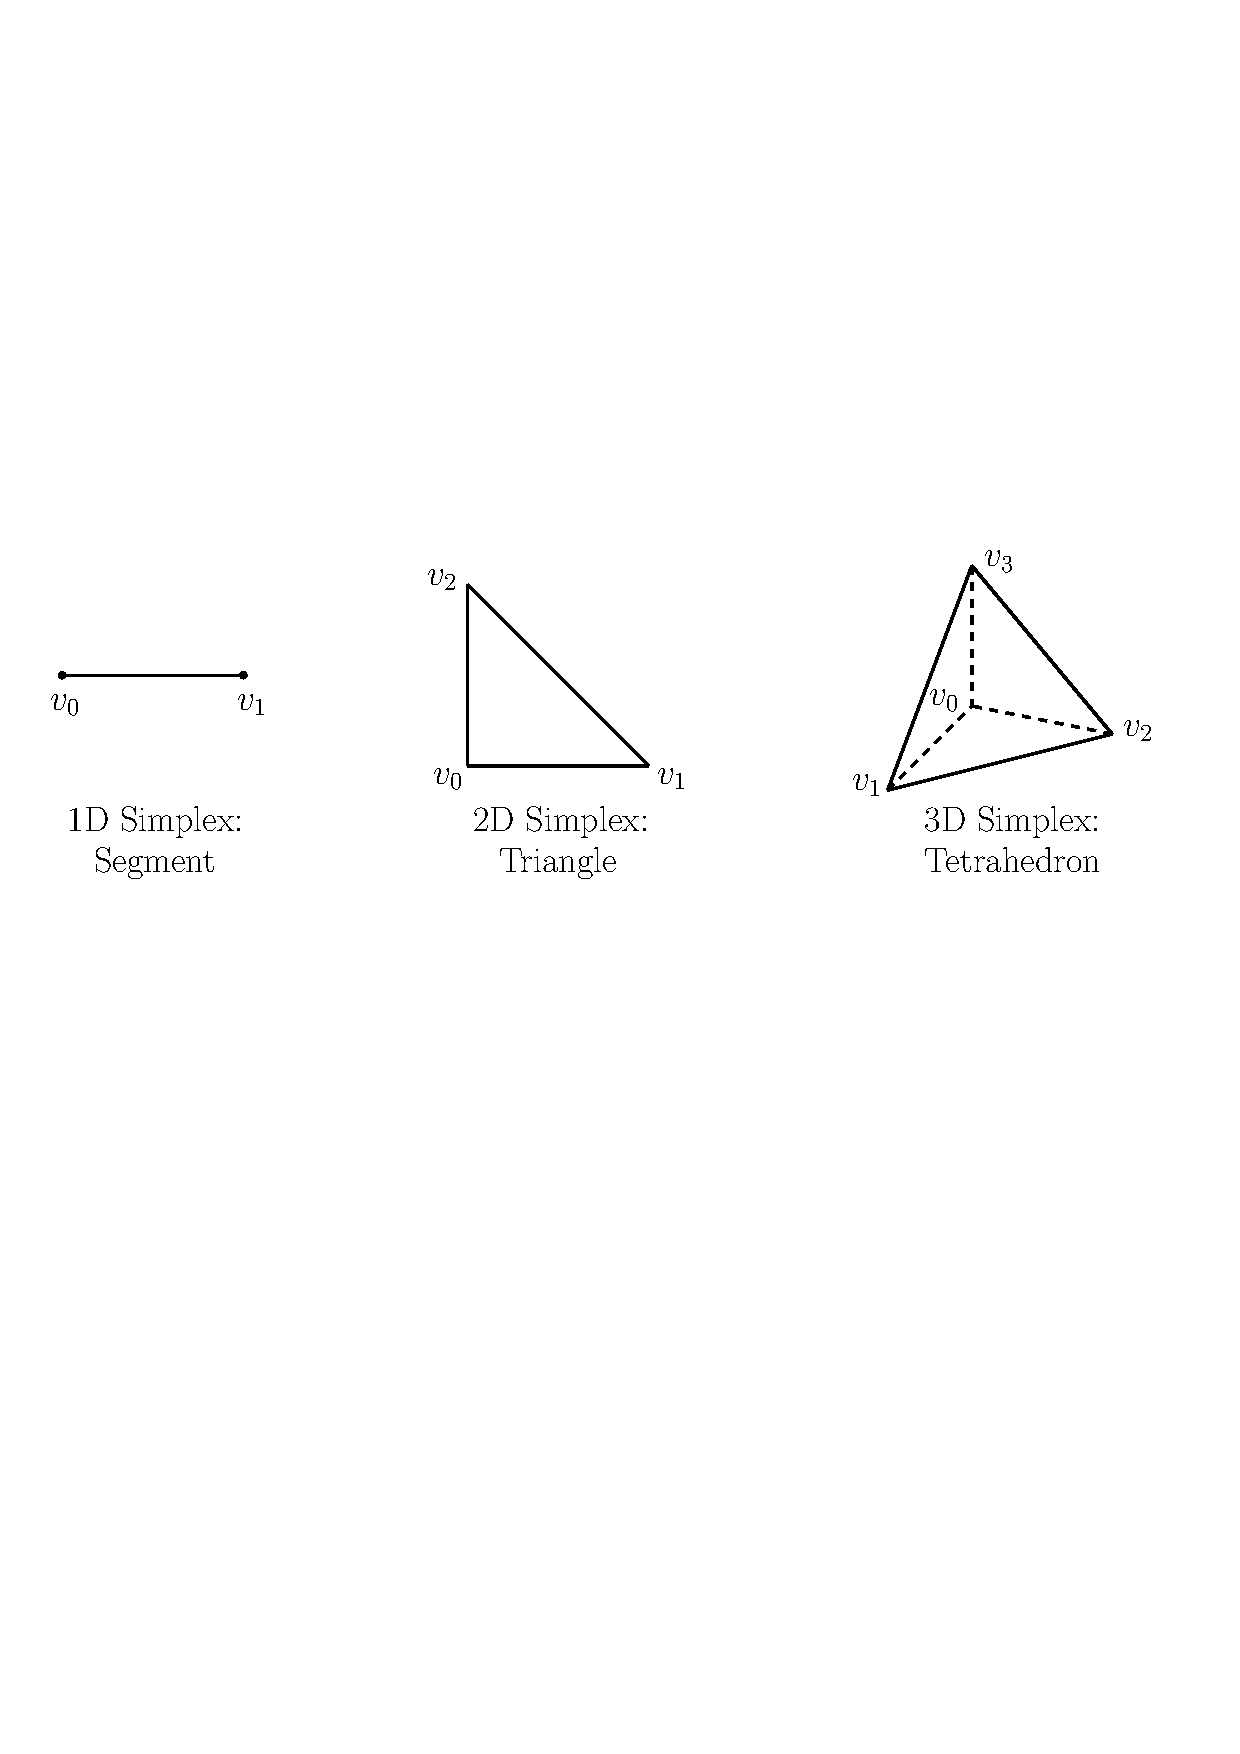
\includegraphics[scale=0.58]{./figures/AffineSimplices.pdf}
\caption{Simplices in 1D, 2D and 3D.}
\label{fig:affinesimplices}
\end{center}
\end{figure}

We now define the affine coordinates.
Let $ v_0,\ldots, v_N$, denote the vertices of some simplex, $\Delta$.
%\footnote{Segment ($N=1$), triangle ($N=2$), tetrahedron ($N=3$), etc.}
Any point $ x\in\Delta$ can be expressed as a convex combination of the vertices:
\begin{equation}
 x = \sum_{a=0}^N s_a v_a\, .\label{eq:affinerepresentation}
\end{equation}
The weights in the sum above, $s_0,\ldots,s_N$, are the affine coordinates for $\Delta$.
We can think of them both as coordinates in and of themselves, or functions of the Cartesian variable $x$. 
Due to being a convex combination, for all $x\in\Delta$ it holds that
\begin{equation}
\sum_{a=0}^N s_a(x)=1\,,\quad\text{ and }\quad s_a(x)\geq0\,.\label{eq:affinesumtoone}
\end{equation}

Throughout this document, to ease the understanding, we shall use the following convention for affine coordinates.
\begin{itemize}
	\item 1D: $\mu_0,\mu_1$ will be affine coordinates for edges ($N=1$, $\mu_a=s_a$ and $a=0,1$).
	\item 2D: $\nu_0,\nu_1,\nu_2$ will be affine coordinates for triangles ($N=2$, $\nu_a=s_a$ and $a=0,1,2$).
	\item 3D: $\lambda_0,\lambda_1,\lambda_2,\lambda_3$ will be affine coordinates for tetrahedra ($N=3$, $\lambda_a=s_a$ and $a=0,1,2,3$).
\end{itemize}
% $\mu_n:=s_n$, $n\in\{0,1\}$  (1D); $\nu_n:=s_n$, $n\in\{0,1,2\}$  (2D); $\lambda_n:=s_n$, $n\in\{0,1,2,3\}$ will denote affine coordinates for the tetrahedron (3D).
We will often use the following ``vector'' notation for compactness:
\begin{equation}
	\vec{s}_{ab}=(s_a,s_b)\,,\quad\qquad\vec{s}_{abc}=(s_a,s_b,s_c)\,,
\end{equation}
where $s=\mu,\nu,\lambda$. Hence, for example, $\vec{\nu}_{12}=(\nu_1,\nu_2)$ and $\vec{\lambda}_{031}=(\lambda_0,\lambda_3,\lambda_1)$.

Explicit formulas  for the affine coordinates (in terms of Cartesian coordinates) used for each element will be given at the beginning of each corresponding section.

% Throughout the text we will use the symbols
% $s_0,s_1,\ldots,s_N$ for $N=1,2,3$ to denote general affine coordinates. When the dimension of the space, $N$, is specified, then whenever possible, we will use the dimension-specific notations
% $\mu_0,\mu_1,\quad \text{in 1D},$
% $\nu_0,\nu_1,\nu_2\quad \text{in 2D},$
% $\lambda_0,\lambda_1,\lambda_2,\lambda_3\quad \text{in 2D},$
%  (define affine coordinates+notation)

\subsection{Outline}

The document will be organized naturally starting with the simplest element in 1D and then, as dimension and complexity increase, leading into the most complicated elements in 3D.
The order of sections is: segment (\S\ref{sec:Segment}), quadrilateral (\S\ref{sec:Quad}), triangle (\S\ref{sec:Tri}), hexahedron (\S\ref{sec:Hexa}), tetrahedron (\S\ref{sec:Tet}), prism (\S\ref{sec:Prism}) and pyramid (\S\ref{sec:Pyramid}).
Those interested only in simplicial elements may simply read segment, triangle and tetrahedron, while those interested only in quadrilateral and hexadedral elements can also skip the nonrelevant sections.
The prism and pyramid sections are better appreciated after reading through all of the previous sections.
As mentioned before, with regard to orientations, for each element there will always be a final subsection describing the necessary notions and modifications to implement orientation embedded shape functions.
Therefore, as a first iteration in trying to implement the shape functions, or for those readers for which this aspect is not of interest, we suggest skipping those subsections.
%These can be skipped by any reader for which this aspect is not of interest.

As a prelude to all the constructions, there is a section introducing the concept of polynomial scaling and the versions of Legendre and Jacobi polynomials used in our constructions.
More importantly, the concept of \textit{homogenization} is defined.
This is fundamental for the elements involving triangle faces (triangle, tetrahedron, prism, and pyramid).

Finally, as mentioned before, a set of tables available in Appendix \ref{app:ShapeFunctionTable} give a thorough definiton of all ancillary functions and shape functions presented in the text.
These tables should be used as a reference by the reader when looking at the provided code or when implementing their own version.
%Finally, should a reader wish immediately to skip the discussions, in Appendix~\ref{app:ShapeFunctionTable}, we provide a table giving a thorough definiton of all shape functions. This table should also be used as a reference when using or trying to implement the code.

\subsection{Previous Work}

Our constructions are often based either in part or in full in previous work by various collaborators in the field.
%The unique aspect here is the unified approach to all four 3D elements for the full sequence.
Construction of shape functions for the quadrilateral follows \citet{AinsworthCoyle01} (see also \citet{hpbook2}).

For the triangle and tetrahedron, our construction is based on the concept of \textit{scaled polynomials} as described by \citet{karniadakisbook}, \citet{Schoeberl_Zaglmayr_05}, \citet{SabineThesis} and the subsequent work of \citet{Beuchler_Pillwein_Schoeberl_Zaglmayr_12}.
%we initially follow the construction of \citet{Schoeberl_Zaglmayr_05} based on the idea of \textit{scaled polynomials}, and the subsequent work of \citet*{Beuchler_Pillwein_Schoeberl_Zaglmayr_12}.
See also \citet{Beuchler_Schoeberl_06, Beuchler_Pillwein_07, Beuchler_Pillwein_Zaglmayr_12} and \citet{Beuchler_Pillwein_Zaglmayr_13} for more details on obtaining good sparsity properties via appropriate selection of Jacobi polynomials.
Contrary to their work, here we study the classical $H(\text{curl})$ and $H(\text{div})$ conforming N\'{e}d\'{e}lec and Raviart-Thomas spaces having the property that they are affine invariant, and being compatible (at the space level) with the spaces proposed for the pyramid.
Other interesting shape functions for the tetrahedron include those of \citet{AinsworthBezier} based on Bernstein polynomials. Lastly, it is worth noting that \citet{SabineThesis} also presents a unified construction of the hexahedron and prism to complement the tetrahedron, but does not include the pyramid.

The prism element is a Cartesian product of the 2D triangle and 1D segment.
The prism shape functions therefore utilize constructs from the triangle and segment.

Construction of pyramid shape functions builds on the fundamental work of \citet{Nigam_Phillips_11} and their first family of pyramid spaces.
The spaces are natural for (parallelogram-based) affine pyramids, but as evidenced by \citet{Bergot_Durufle_14}, they also have other attractive properties in a non-affine setting.
We also note that \citet{Bergot_Gary_Durufle_10} and \citet{Bergot_Durufle_14} have contributed to the work on higher order pyramid shape functions, but their spaces and shape functions are different.
%Due to the pyramid being a connecting element, with very few elements in a typical mesh, our aim here is not to focus on the most optimal spaces for this element, but rather on the theoretical aspects of the commuting exact sequence property which ensure certain interpolation estimates.

The idea of orientation embedded shape functions follows the work of \citet{GattoDemkowicz10} and stems from discussions with Joachim Sch\"oberl dating back to the Vienna WCCM congress in 2002.

%and are compatible with the other classical N\'{e}d\'{e}lec's spaces of the first type.  , but based on this previous work, note the good properties this first family of spaces have in non-affine pyramids.
%We also stress that our aim in this work is not
%, we focus on the classical choice of spaces that contain only \Nedelec's tetrahedral polynomial spaces.
%{\color{red} whose elements?} These elements anticipate use of algebraic mesh generators and may fail to deliver optimal rates or may fail to even converge for general unstructured meshes (see \cite{hpbook2}, p.96, for a detailed discussion).


%\subsection{Outline}
%
%This paper is divided into isolated sections, one for each element the reader may wish to construct. Naturally, each section may require shape functions defined in the previous sections. For instance, to construct shape functions of the tetrahedron element, the reader must first be able to construct its trace spaces and so the segment and triangle element sections are somehow crucial. Naturally, the shape functions one needs for the tetrahedron are defined across the three sections on the segment (\S~\ref{sec:Segment}), the triangle (\S~\ref{sec:Tri}), and, of course, the tetrahedron (\S~\ref{sec:Tet}). However, we urge the reader to note that many sections are, in fact, independent of each other. For instance, if only reading for the tetrahedron, the reader may wish to skip both \S~\ref{sec:Quad} on the quadrilateral and \S~\ref{sec:Hexa} on the hexahedron even though they appear first. The shape functions in those two sections are not necessarily required for the tetrahedron as the geometry is different in each case beyond the level of the edge element.
%
%We advise all readers to read both \S~\ref{sec:Notation} and \S~\ref{sec:Segment}. The material in these sections is common to all elements, although the paricular discussion of Jacobi polynomials in \S~\ref{sec:Notation} is only required for elements having triangular faces.
%
%The shape functions of the pyramid element discussed in \S~\ref{sec:Pyramid} will require sections both \S~\ref{sec:Quad} on the quadrilateral and \S~\ref{sec:Tri} on the triangle. We also encourage the reader to browse \S~\ref{sec:Hexa} on the hexahedron and \S~\ref{sec:Tet} on the tetrahedron before seeking a full understanding of the pyramid element. Our construction for the pyramid is partially motivated by these previous sections.
%
%Should a reader wish immediately to skip to the discussion in any particular element, in Appendix~\ref{app:ShapeFunctionTable}, we provide a table giving a thorough definiton of all shape functions. This table should also be used as a reference when using the code.


%Section 2
\newpage
\section{Polynomials Prelude}
\label{sec:Notation}

\subsection{Notation}

% Our construction is based on a few generating families of polynomials. Their general properties are discussed in Appendix~\ref{app:GeneratingFamilies}.
% In this work, we will use Legendre and Jacobi polynomials.

% The reader will observe that all of the formulas in this section are derived for two certain specified sets of polynomials. Should the reader wish to work with different sets of polynomials, our construction generalizes as discussed in Appendix~\ref{app:GeneratingFamilies}. Therefore, it is certainly not necessary that the constructions of shape functions presented in the later sections require the specific polynomials we have decided to use in our own implementation.

The polynomials of order $p$ with arguments $x\in\mathbb{R}$ will be denoted by
\begin{equation}
   	\mathcal{P}^p(x)=\mathrm{span}\{x^j:j=0,\ldots,p\}\,.
\end{equation}
Similarly, in two dimensions  the polynomials of total order $p$ with arguments $(x,y)\in\mathbb{R}^2$ are denoted by
\begin{equation}
    \mathcal{P}^p(x,y)=\mathrm{span}\{x^iy^j:i\geq0,j\geq0,n=i+j\leq p\}\,,
\end{equation}
while the \textit{homogeneous} polynomials of total order $p$ are denoted by
\begin{equation}
    \tilde{\mathcal{P}}^p(x,y)=\mathrm{span}\{x^iy^j:i\geq0,j\geq0,i+j=p\}\,.
\end{equation}
Similar definitions apply to polynomials of three variables. 
Moreover, when the domain is clear from the context, we will simply refer to $\mathcal{P}^p(x,y)$ and $\tilde{\mathcal{P}}^p(x,y)$ as $\mathcal{P}^p$ and $\tilde{\mathcal{P}}^p$ respectively.

Define
\begin{equation}
 \mathcal{Q}^{p,q}(x,y)=\mathcal{P}^p(x)\otimes\mathcal{P}^q(y)
        =\spann\{x^i y^j \,:\,0\leq i\leq p,\:0\leq j\leq q\}\,,
\end{equation}
and similarly for $\mathcal{Q}^{p,q,r}(x,y,z)$. When the variables are clear from the context, these spaces are simply written as $\mathcal{Q}^{p,q}$ and $\mathcal{Q}^{p,q,r}$ respectively.

The notation for vector valued polynomial spaces will be
\begin{equation}
	(\mathcal{P}^p)^2 = \mathcal{P}^p\times\mathcal{P}^p\,,
\end{equation}
and similarly for $\left(\mathcal{P}^p\right)^3$, and the vector valued homogeneous polynomials, $(\tilde{\mathcal{P}}^p)^N$, $N=2,3$.

\subsection{Scaled Polynomials}

Given an order $i$ univariate polynomial, $\psi_i(x)\in\mathcal{P}^i(x)$, we define the corresponding {\em scaled polynomial}
\begin{equation}
	\psi_i(x; t) = \psi_i\Big(\frac{x}{t}\Big) t^i \, .
	\label{eq:scaledpolyomials}
\end{equation}
% The definition extends to polynomials in many variables. If $\psi_i(x,y)$ is a polynomial of (total) order $i$, then
% \be
% \psi_i(x,y;t) := \psi_i( \frac{x}{t}, \frac{y}{t}) \, t^i \, .
% \ee
% Obviously, $\psi_i(x;1) = \psi_i(x)$ and $\psi_i(x,y,; 1) = \psi_i(x,y)$, so the scaled polynomials define polynomial extensions into the $x,t$ or $x,y,t$ space.
Obviously, $\psi_i(x;1) = \psi_i(x)$, so the scaled polynomials define two variable polynomial extensions into the $(x,t)$ space.
Furthermore, the reader may observe that $\psi_i(x;t)$ is homogenous of order $i$ as a polynomial in this space, i.e. $\psi_i(x;t)\in\tilde{\mathcal{P}}^i(x,t)$.

\subsection{Legendre Polynomials}
\label{sec:LegendrePol}

In this work, we will use Legendre and Jacobi polynomials for the construction of all shape functions. Should the reader wish to work with different families of polynomials, our construction easily generalizes as discussed in Appendix~\ref{app:GeneratingFamilies}.

The classical Legendre polynomials comprise a specific orthogonal basis for $L^2(-1,1)$. Truncated to the first $p$ elements, $\{\tilde{P}_i:i=0,\ldots,p-1\}$, the Legendre polynomials\footnote{Although the common notation for the classical Legendre polynomials is $P_i$, we choose to denote the elements in this set with $\sim$ as we will only need this definition temporarily.} are a basis for the space of (single variable) polynomials of order $p-1$.

Of many properties of the Legendre polynomials, we list the following recursion formula
\begin{equation}
\begin{aligned}
	\tilde{P}_0(y)&=1\,,\\
	\tilde{P}_1(y)&=y\,,\\
	i\tilde{P}_i(y)&=(2i-1)y\tilde{P}_{i-1}(y) - (i-1)\tilde{P}_{i-2}(y)\,, \quad \text{for }\, i\geq2\,,
\end{aligned}
\label{eq:recursion1}
\end{equation}
and the derivative formula for $i\geq1$,
\begin{equation}
(2i+1) \tilde{P}_i(y) = \frac{\partial}{\partial y} \Big(\tilde{P}_{i+1}(y)-\tilde{P}_{i-1}(y)\Big)\,,
\label{eq:Dervivative1}
\end{equation}
which are both well known in the literature. We also make note of the $L^2$ orthogonality relationship
\begin{equation}
\int_{-1}^{1} \tilde{P}_i(y)\tilde{P}_j(y)\,\mathrm{d}y=0\,, \quad \text{if } i\neq j\,.
\label{eq:Orthogonality1}
\end{equation}
This relationship, and the definition $\tilde{P}_0(y) = 1$, leads to the zero average property
\begin{equation}
\int_{-1}^{1} \tilde{P}_i(y)\,\mathrm{d}y=0\,, \quad \text{for } i\geq1\,.
\label{eq:ZeroAverage1}
\end{equation}

\paragraph{Shifting.}
The range of affine coordinates is always $[0,1]$ (see \eqref{eq:affinesumtoone}).
Although not clear at the moment, this implies that we want to have the zero average property over the interval $[0,1]$ instead of $[-1,1]$.
We can obtain this property by composing each Legendre polynomial above with the shifting operation
%More importantly, the range of the affine shape functionsTherefore, because of how we have defined our master elements, we will wish to have a similar set of polynomials with the zero average property over the interval $[0,1]$ instead of $[-1,1]$. We can form such a set of polynomials by composing each Legendre polynomial above with the shifting operation
\begin{equation}
y \mapsto 2x-1\,.
\label{eq:shift}
\end{equation}
The (shifted) Legendre polynomials over $[0,1]$ are defined for $i\geq0$,
\begin{equation}
P_i(x) = \tilde{P}_i\left(2x-1\right)\,.
\end{equation}

% \paragraph{Shifted, scaled Legendre polynomials.}

% With $P_i(x)$ denoting Legendre polynomials, the corresponding {\em scaled Legendre polynomials}
% are:
% \be
% P_i(x;t) = P_i(\frac{x}{t}) t^i \, .
% \ee
% A well-known recursive formula for Legendre polynomials extend easily to the scaled Legendre polynomials. The definition of scaled polynomials implies:
% \be
% \begin{array}{rl}
% P_0(x;t)    &=\, 1 \,,\\[2pt]
% P_1(x;t)    &=\, x \,,\\[2pt]
% i P_i(x; t) &=\, (2i-1) x  P_{i-1}(x; t) - (i-1)t^2 P_{i-2}(x; t)\,, \quad \text{for }\, i\geq2\, .
% \end{array}
% \label{eq:recursion1}
% \ee
% % Commutativity of scaling and differentiation in $x$ implies that:
% % \be
% % (2i+1)P_i(x; t) = \frac{\ptl }{\ptl x} \left(P_{i+1}(x; t) - t^2 P_{i-1}(x; t)\right) \, .
% % \label{eq:recursion2}
% % \ee

% Note that since the the Legendre polynomials are orthogonal with respect to the $L^2$ inner product on the interval $(-1,1)$,
% % \be
% % 0 = \int\limits_{-1}^{1} P_i(x)P_j(x), \quad \text{if } i\neq j\,,
% % \ee
% the scaled Legendre polynomials are, in turn, orthogonal with respect to the $L^2$ inner product on the interval $(-t,t)$
% \be
% \int\limits_{-t}^{t} P_i(x;t)P_j(x;t)\:dx=0\,, \quad \text{if } i\neq j\,.
% \ee

\paragraph{Scaling.}
% In the coming constructions of shape functions involving simplicial geometries (traingle, tetrahedron, prism, and pyramid), we also require a one parameter set of basis polynomials with the zero-average property on the interval $(0,t)$, $t\in(0,1)$. We may generate this set from the above shifted Legendre polynomials by the shifting operation defined above
The (shifted) scaled Legendre polynomials are defined by \eqref{eq:scaledpolyomials} as
\begin{equation}
	P_i(x;t) = P_i\left(\frac{x}{t}\right)t^i = \tilde{P}_i\left(2\left(\frac{x}{t}\right)-1\right)t^i = \tilde{P}_i(2x-t;t) \,,
\end{equation}
where the domain in $x$ is $[0,t]$.

This set of scaled Legendre polynomials obeys a recursion formula similar to (\ref{eq:recursion1}):
\begin{equation}
	\begin{aligned}
		P_0(x;t)&=1 \,,\\
		P_1(x;t)&=2x-t \,,\\
		iP_i(x;t)&=(2i-1)( 2x - t) P_{i-1}(x; t) - (i-1)t^2 P_{i-2}(x; t) \,, \quad \text{for }\, i\geq2\, .
	\end{aligned}
\label{eq:recursion2}
\end{equation}
Moreover, we carry over the orthogonality and zero average properties from \eqref{eq:Orthogonality1} and \eqref{eq:ZeroAverage1} to the scaled domain $[0,t]$:
\begin{equation}
	\begin{gathered}
		\int_{0}^{t} P_i(x;t)P_j(x;t)\,\mathrm{d}x=0\,, \quad \text{if } i\neq j\,,\\
		\int_{0}^{t} P_i(x;t)\,\mathrm{d}x=0\,, \quad \text{for } i\geq1\,.
	\end{gathered}
	\label{eq:ZeroAverage2}
\end{equation}
%which implies the zero-average property,
%\be
%\int\limits_{0}^{t} P_i(x;t)\:dx=0\,, \quad \text{for all } i\geq1\,.
%\label{eq:ZeroAverage2}
%\ee

\paragraph{Integrated Legendre Polynomials.}

% Defining
% \be
% L_0(x;t) = 1-x\,,
% \ee
% w
For all $i\geq1$, we define the (scaled) integrated Legendre polynomials,
\begin{equation}
	L_{i}(x; t) = \int_0^{x} P_{i-1}(\tilde{x}; t)\, \mathrm{d}\tilde{x}\,,
\end{equation}
where of course $L_i(x)=L_i(x;1)$. Notice that $\mathcal{P}^{p}(x)=\mathrm{span}(\{1\}\cup\{L_i:i=1,\ldots,p\})$. By construction, the $L_i$ are seen as elements of $H^1$ and as a result, their pointwise evaluation is understood to be well defined. Therefore, recalling the zero average property of the Legendre polynomials, we observe that,
% \footnote{By this observation, for each $i\geq2$, we may factor the product $x(x-1)$ from each $L_i(x)$.}
\begin{equation}
	L_i(0)=L_i(0;t)=0=L_i(t;t)=L_i(1)\,,\quad\text{for }\,i\geq2\,.\label{eq:Lvanishatendpoints}
\end{equation}

Next, \eqref{eq:Dervivative1} motivates the formulas for computing the integrated Legendre polynomials:
\begin{equation}
	\begin{aligned}
		L_1(x;t)&=x\,,\\
		2(2i-1) L_i(x; t)&=P_i(x; t) - t^2 P_{i-2}(x; t) \,, \quad\text{for }\, i\geq2\,.
	\end{aligned}
	\label{eq:shifted_scaled_lobatto}
\end{equation}
% By definion,
% \be
% \frac{\ptl}{\ptl x'} L_{i+1}(x; t) = P_i(x; t)\,.
% \ee
% From~(\ref{eq:shifted_scaled_lobatto}) we get:
% \be
% (2i+1) \frac{\ptl}{\ptl t} L_{i+1}(x; t) =
% \half \left( \frac{\ptl}{\ptl t}  {P}_{i+1}(x; t)
% - 2t P_{i-1}(x; t) - t^2 \frac{\ptl}{\ptl t} P_{i-1}(x; t)
% \right) \, ,
% \ee
% with derivatives in $t$ evaluated through the recursion:
% \be
% \begin{array}{rll}
% i\frac{\ptl}{\ptl t}  {P}_i(x; t)   = &
% (2i-1)& \left( - {P}_{i-1}(x; t) + (2x - t) \frac{\ptl}{\ptl t} P_{i-1}(x; t) \right)
% \\[8pt]
%  - &(i-1) &
% \left(
% 2t P_{i-2}(x; t) + t^2 \frac{\ptl}{\ptl t}   {P}_{i-2}(x; t)
% \right)\, .
% \end{array}
% \ee

Clearly,
\begin{equation}
	\frac{\partial}{\partial x} L_{i}(x; t) = P_{i-1}(x; t)\,.
\end{equation}
Derivatives of $L_i(x;t)$ with respect to $t$ will also be necessary in our computations.
For this, we define
\begin{equation}
	R_i(x) = (i+1)L_{i+1}(x) - xP_i(x)\,,\quad\text{for }\, i\geq0\,,
	\label{eq:RDef}
\end{equation}
which the reader may observe is an order $i$ polynomial. In Appendix~\ref{app:GeneratingFamilies} we show that
\begin{equation}
	\frac{\partial}{\partial t} L_i(x;t) = R_{i-1}(x;t)\,.
\end{equation}
Obviously $R_0(x;t)=0$, and by use of \eqref{eq:recursion2} and \eqref{eq:shifted_scaled_lobatto}, one can reduce \eqref{eq:RDef} to
\begin{equation}
	R_i(x;t) = -\frac{1}{2} \Big(P_i(x;t)+tP_{i-1}(x;t)\Big)\,,\quad\text{for }\,i\geq1\,.
\end{equation}

\subsection{Jacobi Polynomials}

Motivated by \citet{Beuchler_Schoeberl_06} and \citet{Beuchler_Pillwein_07}, we use Jacobi polynomials in our constructions of elements involving triangle faces.
The (shifted to $[0,1]$) Jacobi polynomials, $P^{(\alpha,\beta)}_i(x)$, $\alpha,\beta>-1$, form a two parameter family of polynomials including the Legendre polynomials previously defined ($P_i^{(0,0)} = P_i$). %\footnote{$P_i^{(0,0)} = P_i$ for all $i\geq0$.}
Jacobi polynomials have similar recursion formulas as the Legendre polynomials.
One may find a selection of such formulas in \citet{Beuchler_Pillwein_07}.
For our purposes, we will only consider the case $\beta=0$, so that from now on $P_i^\alpha=P_i^{(\alpha,0)}$.

Jacobi polynomials are also orthogonal in a weighted $L^2$ space. Assuming the scaling operation discussed previously, we have the orthogonality relation
%\footnote{i.e. we define $$P_i^\alpha(x) := \tilde{P}_i^\alpha(2x-1)\,,$$ where $\tilde{P}_i^\alpha$ is the classical Jacobi polynomial on $[-1,1]$.}
\begin{equation}
	\int_{0}^{t} x^\alpha P_i^\alpha(x;t)P_j^\alpha(x;t)\,\mathrm{d}x=0\,, \quad \text{if } i\neq j\,,
\end{equation}
which for $\alpha\neq0$ no longer implies the zero average property.

The following is the recursion formula we use to compute the $[0,t]$ Jacobi polynomials:
% $$
% \begin{array}{c}
% \begin{array}{rl}
%  {P}_0^\alpha(x;t) = & 1 \\[2pt]
%  {P}_1^\alpha(x;t) = & (2+\alpha)x-t\\[2pt]
% \end{array}\\
% a_i  {P}_i^\alpha(x;t)
% = b_i \left( 2c_i x + (\alpha^2-c_i) t \right) P_{i-1}^\alpha(x;t)
% - d_i t^2 P_{i-2}^\alpha(x;t)
% \end{array}
% $$
\begin{equation}
	\begin{aligned}
		P_0^\alpha(x;t) &= 1\,, \\
		P_1^\alpha(x;t) &= 2x-t+\alpha x\,,\\
		a_i {P}_i^\alpha(x;t) &= b_i \left( c_i(2x-t) + \alpha^2 t \right) P_{i-1}^\alpha(x;t) - d_i t^2 P_{i-2}^\alpha(x;t)\,,
		\quad \text{for }\, i\geq2\, ,
	\end{aligned}
\label{eq:RecursionJacobi}
\end{equation}
where
\begin{equation*}
	\begin{aligned}
		a_i &=  2i(i+\alpha)\, (2i + \alpha - 2)\,,\\
		b_i &=  2i + \alpha - 1\,,\\
		c_i &=  (2i+\alpha)\, (2i + \alpha - 2)\,,\\
		d_i &=  2(i+\alpha-1)\, (i-1)\, (2i+\alpha)\,.
	\end{aligned}
\end{equation*}

We remark that other recursive relations in weight and order to compute Jacobi polynomials, such as $(\alpha+i)P_i^\alpha(x;t)=(\alpha+2i)P_i^{\alpha-1}(x;t)+itP_{i-1}^\alpha(x;t)$, were experimentally found to be numerically unstable as compared to fixing a value of $\alpha$ and using \eqref{eq:RecursionJacobi}, so that the latter approach is recommended.
% All discussed definitions extend to general Jacobi polynomials $P^{(\alpha,\beta)}_i(x)$. The
% scaled Jacobi Polynomials are evaluated using the following recursion.
% $$
% \begin{array}{c}
% \begin{array}{rl}
%  {P}_0^{(\alpha,\beta)}(x;t) = & 1 \\[8pt]
%  {P}_1^{(\alpha,\beta)}(x;t) = & \half \left( (\beta+1)(x - t) + (\alpha+1) (x +t) \right)\\[8pt]
% \end{array}\\
% a_i  {P}_i^{(\alpha,\beta)}(x;t)
% = b_i \left( c_i x + (\alpha^2 - \beta^2) t \right) P_{i-1}^{(\alpha,\beta)}(x;t)
% - d_i t^2 P_{i-2}^{(\alpha,\beta)}(x;t)
% \end{array}
% $$
% where
% $$
% \begin{array}{rl}
% a_i = & 2i(i+\alpha+\beta)\, (2i + \alpha + \beta - 2)\\
% b_i = & 2i + \alpha + \beta - 1\\
% c_i = & (2i+\alpha+\beta)\, (2i + \alpha + \beta - 2)\\
% d_i = & 2(i+\alpha-1)\, (i+\beta-1)\, (2i+\alpha+\beta)
% \end{array}
% $$
% For $\alpha=\beta=0$, we recover the formulas for Legendre polynomials. The shifted scaled Jacobi
% polynomials are defined by:
% $$
% \tilde{P}^{(\alpha,\beta)}_i(x;t) = P^{(\alpha,\beta)}_i(2x-t;t) \, .
% $$
% We shall use only the Jacobi polynomials with non-zero weight $\alpha$, i.e.
% $ {P}^{\alpha}_i :=  {P}^{(\alpha,0)}_i$.


% As we will need Jacobi polynomials with weight $\alpha$ varying with the polynomial degree $i$, we shall also use an alternate recursion in both weight and degree,
% \be
% (\alpha +i) \tilde{P}^{\alpha}_i(x;t) =  (\alpha + 2i) \tilde{P}^{\alpha-1}_i(x;t) + i t \tilde{P}^{\alpha}_{i-1}(x;t) \, .
% \ee


\paragraph{Integrated Jacobi Polynomials.}
Finally, we define the (scaled) integrated Jacobi polynomials for $i\geq1$:
\begin{equation}
	L^{\alpha}_i(x;t) = \int_0^x P^{\alpha}_{i-1} (\tilde{x};t) \, \mathrm{d}\tilde{x} \, ,
\end{equation}
with $L^{\alpha}_i(x)=L^{\alpha}_i(x;1)$. Note that because of the absence of the zero average property, we cannot deduce that $L^\alpha_i(1)=0$, and in general, this does not hold. However, it is obvious that for all $\alpha>-1$,
\begin{equation}
	L^\alpha_i(0)=L^\alpha_i(0;t)=0\,,\quad\quad\text{for }\,i\geq1\,.\label{eq:Lalphavanishzero}
\end{equation}

We evaluate the integrated Jacobi polynomials using the following relations:\footnote{cf. (2.9) in \citet{Beuchler_Pillwein_07}.}
\begin{equation}
	\begin{aligned}
		L^{\alpha}_1(x;t) & = x\,, \\
		L^{\alpha}_i(x;t) & = a_i P^{\alpha}_i(x,t) + b_i t P^{\alpha}_{i-1}(x;t)- c_i t^2 P^{\alpha}_{i-2}(x;t)\,,
			\quad\text{for }\, i\geq2\,,
	\end{aligned}
	\label{eq:IntegratedJacobiFormula}
\end{equation}
where
\begin{equation*}
	\begin{aligned}
		a_i = & \frac{i + \alpha}{(2i + \alpha -1)(2i + \alpha)}\,, \\
		b_i = & \frac{\alpha}{(2i + \alpha -2)(2i + \alpha)}\,, \\
		c_i = & \frac{i-1}{(2i + \alpha -2)(2i + \alpha-1)}\,.
	\end{aligned}
\end{equation*}

As in the case of the integrated Legendre polynomials, we find that
\begin{equation}
\frac{\partial }{\partial x}L^\alpha_{i}(x;t) = P^\alpha_{i-1}(x;t)\,,\qquad\quad\frac{\partial}{\partial t} L^\alpha_{i}(x;t) = R^\alpha_{i-1}(x;t)\,,
\end{equation}
where again,
\begin{equation}
	R^\alpha_i(x) = (i+1)L^\alpha_{i+1}(x) - xP^\alpha_i(x)\,.
\label{eq:RalphaDef}
\end{equation}
% we again have
% \be
% \frac{\ptl}{\ptl t} L^\alpha_i(x;t) = R^\alpha_{i-1}(x;t)\,.
% \ee
Obviously $R^\alpha_0(x;t)=0$, and by use of \eqref{eq:RecursionJacobi} and \eqref{eq:IntegratedJacobiFormula}, one can reduce \eqref{eq:RalphaDef} to\footnote{cf. (2.16) in \citet{Beuchler_Pillwein_07}.}
\begin{equation}
	R^\alpha_i(x;t) = -\frac{i}{2i+\alpha} \Big(P^\alpha_i(x;t)+tP^\alpha_{i-1}(x;t)\Big)\,,\quad\text{for }\,i\geq1\,.
\end{equation}


\subsection{Homogenization}

\begin{definition*}
For an order $i$ polynomial
\begin{equation*}
	\psi_i \in \mathcal{P}^i(s_1,\ldots,s_d)\,,
\end{equation*}
we define the operation of homogenization $($of order $i$$)$ as a linear transformation
\begin{equation}
 [\,\cdot\,]:\mathcal{P}^i(s_1,\ldots,s_d) \longrightarrow \tilde{\mathcal{P}}^i(s_0,s_1,\ldots,s_d)\,,
\end{equation}
where
\begin{equation*}
	[\psi_i](s_0,s_1,\ldots,s_d)=\psi_i\left(\frac{s_1}{s_0+\cdots+s_d},\ldots,\frac{s_d}{s_0+\cdots+s_d}\right)\,(s_0+\cdots+s_d)^i\,.
\end{equation*}
\end{definition*}

Notice that homogenization is a form of scaling, and as such, it is forming an extension of the particular case in which $s_0+s_1\cdots+s_d=1$.
It is not a coincidence that this is precisely the property that affine coordinates satisfy (see \eqref{eq:affinesumtoone} in \S\ref{sec:affinecoordinates}).
Moreover, note that $[\psi_i]$ is always a homogeneous polynomial of degree $i$, so we have the following scaling property for all scalars $\gamma$,
\begin{equation}
	[\psi_i](\gamma s_0,\gamma s_1,\ldots,\gamma s_d) = \gamma^i [\psi_i](s_0,s_1,\ldots,s_d)\,.
	\label{eq:ScalingProperty}
\end{equation}

One will observe that for the particular case $d=1$,
\begin{equation}
	[\psi_i](s_0,s_1) = \psi_i(s_1;s_0+s_1)\, .
	\label{eq:univariate}
\end{equation}
Therefore, we see that
\begin{equation}
	[\psi_i](s_0,s_1) = \psi_i(s_1;1) = \psi_i(s_1) \,,\quad \quad\text{if }\,s_0+s_1=1\,,
	\label{eq:homogfor1Daffine}
\end{equation}
where we remind the reader that the 1D affine coordinates satisfy precisely this property.

Moreover, take the case of the integrated Legendre polynomials and recall property \eqref{eq:Lvanishatendpoints}. It follows that for all $s_0,s_1$,
\begin{equation}
	[L_i](s_0,0)=L_i(0;s_0)=0=L_i(s_1;s_1)=[L_i](0,s_1)\,,\quad\text{for }\,i\geq2\,.\label{eq:Lhomogvanishatendpoints}
\end{equation}

In the $d=2$ case, one can make another useful observation.
Let $\chi_j$ be a one variable polynomial of order $j$, and consider the homogenization of the $i+j$ order (two variable) polynomial
\begin{equation}
	\psi_{ij}(s_0,s_1) = [\psi_i](s_0,s_1)\chi_j(1-s_0-s_1)\,.
\end{equation}
In this case, using \eqref{eq:ScalingProperty}, we find
\begin{equation}
	\begin{aligned}
		{}[\psi_{ij}](s_2,s_0,s_1)&=[\psi_i]\Big(\frac{s_0}{s_0+s_1+s_2},\frac{s_1}{s_0+s_1+s_2}\Big)
				\chi_j\Big(1-\frac{s_0+s_1}{s_0+s_1+s_2}\Big)(s_0+s_1+s_2)^{i+j}\\
			&=\frac{1}{(s_0+s_1+s_2)^{i}}[\psi_i](s_0,s_1)\chi_j\Big(\frac{s_2}{s_0+s_1+s_2}\Big)(s_0+s_1+s_2)^{i+j}\\
			&=[\psi_i](s_0,s_1)[\chi_j](s_0+s_1,s_2)\,.%\\
			%&=\psi_i(s_1;s_0+s_1)\,\chi_j(s_2;s_0+s_1+s_2)\,.
			\label{eq:homogproduct}
	\end{aligned}
\end{equation}
This inspires the following definition for single variable polynomials, $\psi_i$ and $\chi_j$, of order $i$ and $j$ respectively:
\begin{equation}
	[\psi_i,\chi_j](s_0,s_1,s_2)= [\psi_i](s_0,s_1)[\chi_j](s_0+s_1,s_2)\,,
\end{equation}
where it is clear $[\psi_i,\chi_j]\in\tilde{\mathcal{P}}^{i+j}(s_0,s_1,s_2)$ is a homogeneous polynomial of order $i+j$.

%We now introduce the final notation of this section. , we define the $i+j$ order, homogeneous polynomial
Again, observe that
\begin{equation}
	[\psi_i,\chi_j](s_0,s_1,s_2)=[\psi_i](s_0,s_1)\chi_j(s_2)\,,\quad\quad\text{if }\,s_0+s_1+s_2=1\,,
\end{equation}
where we remind the reader that the 2D affine coordinates satisfy precisely this property.

Finally, using properties \eqref{eq:Lvanishatendpoints} and \eqref{eq:Lalphavanishzero} of the integrated Legendre and Jacobi polynomials, it follows that for all $s_0,s_1,s_2$,
\begin{equation}
	[L_i,L_j^\alpha](s_0,s_1,0)=[L_i,L_j^\alpha](s_0,0,s_2)=[L_i,L_j^\alpha](0,s_1,s_2)=0\,,\quad\text{for }\,i\geq2\,,\,j\geq1\,.
	\label{eq:LiLjvanishing}
\end{equation}

% We now construct an equivalence relation that will be useful in the coming construction of shape functions.
% For a polynomial $\psi_i(x,y)$ of total degree equal to $i$ in $x,y$,
% the corresponding {\em homogenized polynomial} $[\psi_i]$ is defined as:
% \be
% [\psi_i](x,y) := \psi_i(\frac{x}{x+y},\frac{y}{x+y}) \, (x+y)^i \, .
% \ee
% Obviously, $[\psi_i](x,y)$ is a homogeneous polynomial of order $i$.% and we note that this forms an equivalence class of polynomials of degree $i$.
% Similarly, the operation $[\,\cdot\,]:\mathcal{P}^i\to {\mathcal{P}}^i$, can be extended to polyomials of three arguments. For a polynomial $\psi_i(x,y,z)$,
% \be
% [\psi_i](x,y,z) := \psi_i(\frac{x}{x+y+z},\frac{y}{x+y+z},\frac{z}{x+y+z}) \, (x+y+z)^i \, ,
% \ee
% is then a projection to a homogeneous polynomials of order $i$ in three space dimensions.

% Note that if $\psi_i(x,y) = \hat\psi(y)$ is univariate but considered as a polynomial in two dimensions, then homogenization is equivalent to scaling by the factor $t=x+y$,
% \be
% [\psi_i](x,y) = \hat\psi(y;x+y)\, .
% \label{eq:univariate}
% \ee

% Example::: (to edit)

% Observe that the second Lobatto polynomial may be written in more than one different way as a function $\mu_0,\,\mu_1$:
% \be
% L_2(\xi) = 2(\xi-1)\xi = 2\mu_0(\xi)\mu_1(\xi) = 2(1-\mu_1(\xi))\mu_1(\xi)\,,
% \ee
% where still other possibilities are also available. Although the affine functions (themselves taking as arguments affine coordinates, $\mu_0,\,\mu_1$) are different, their evaluation (as a function in $\xi$) on the edge is, in fact, identical.

% Let $p\geq2$ be the order of the edge and let $\hat\phi_i(\xi), \xi \in \e$, be a polynomial of order $2\leq i\leq p$, vanishing at $\xi = 0,1$.
% In general, we can represent function $\hat\phi_i$ in the form:
% \be
% \hat\phi_i(\xi) = \phi_i (\mu_0,\mu_1)
% \ee
% where function $\phi_i$ is a polynomial of (total) degree $i$ in terms of the edge affine coordinates $\mu_0,\mu_1$.

%Section 3
\newpage
\section{Segment}
\label{sec:Segment}

\begin{figure}[!ht]
\begin{center}
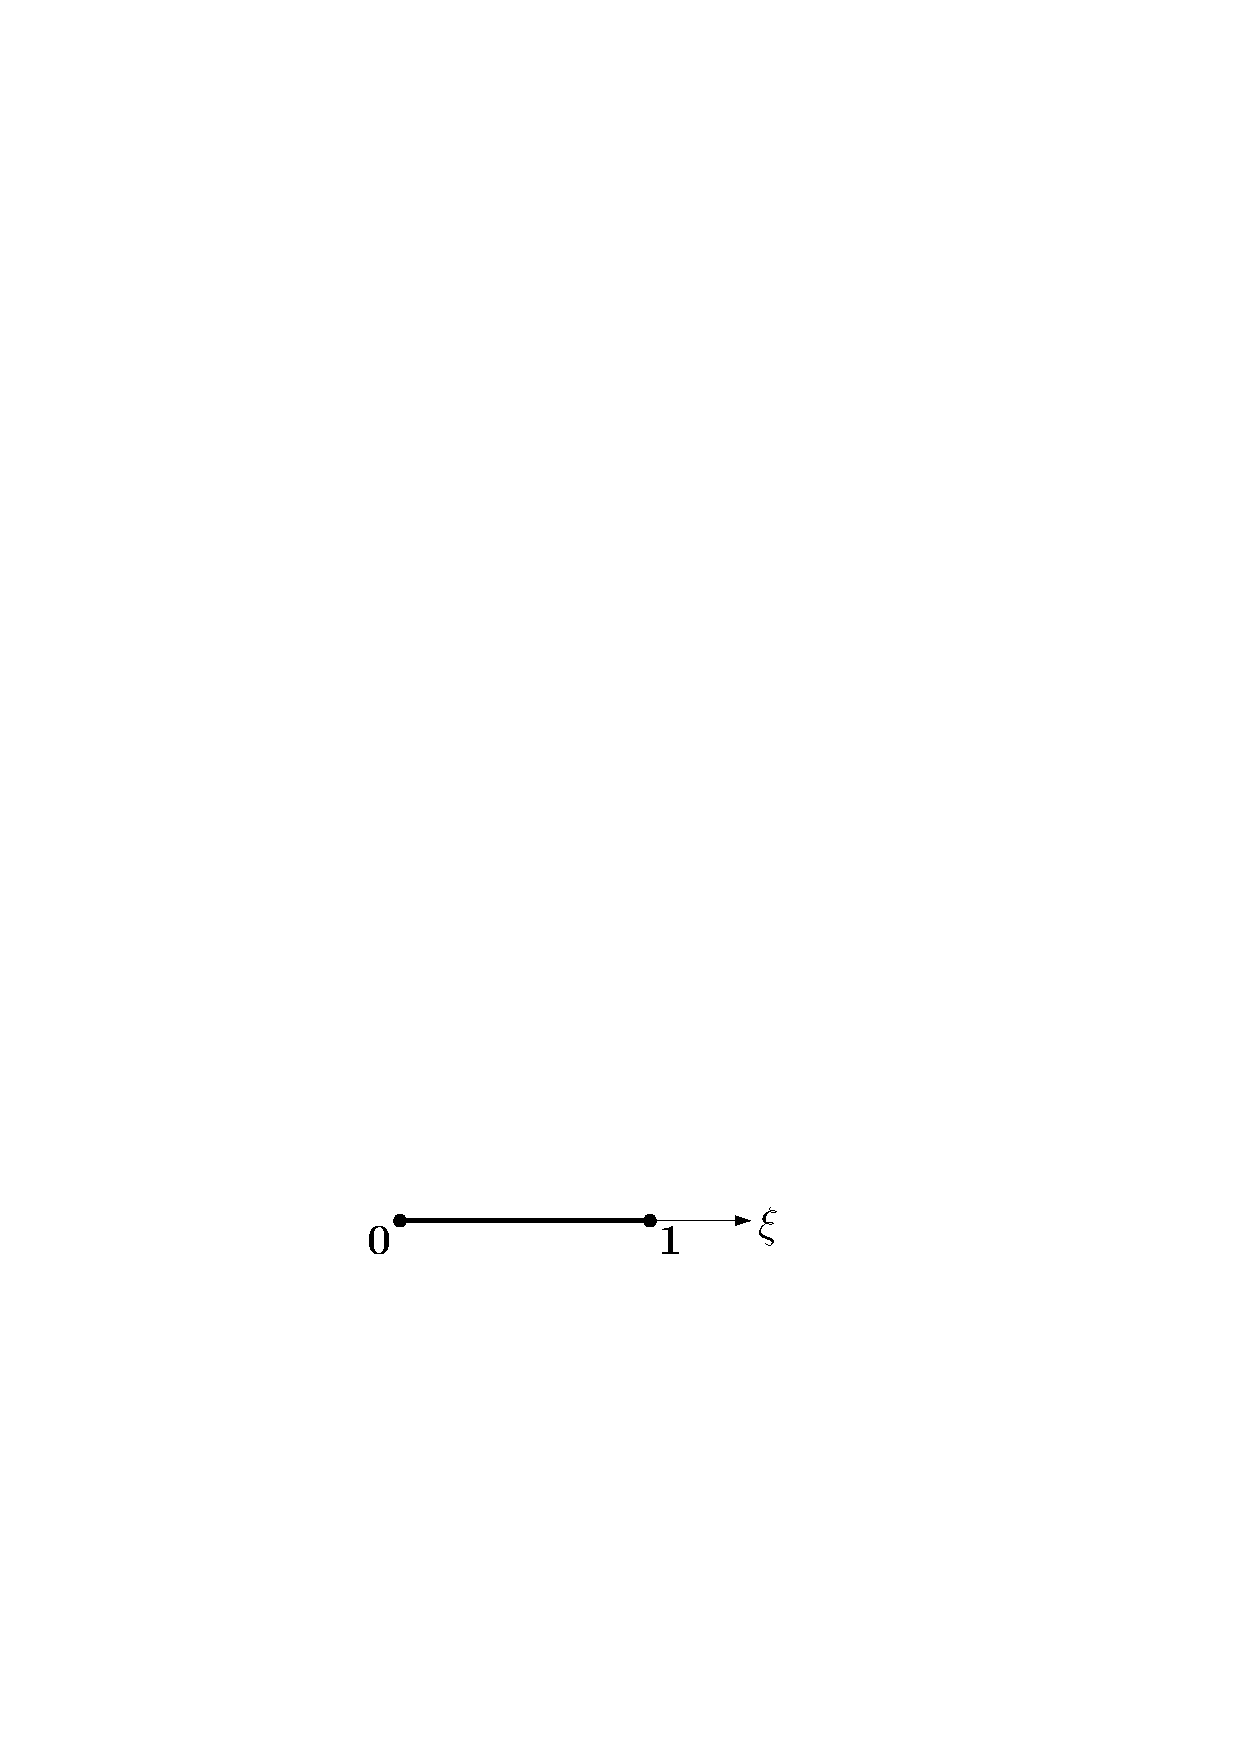
\includegraphics[scale=0.5]{./figures/MasterSegment.pdf}
\caption{Master segment with numbered vertices.}
\label{fig:masterseg}
\end{center}
\end{figure}

The 1D simplex is the segment or edge. 
The master element is defined as the unit interval $(0,1)$, and it is illustrated in Figure \ref{fig:masterseg} with a parameterization given by $\xi\in[0,1]$.

Denote vertex $a$ by $v_a$.
The definition of affine coordinates (see \eqref{eq:affinerepresentation}) states that $\xi=\mu_0(\xi)v_0+\mu_1(\xi)v_1$, with $\mu_0(\xi)+\mu_1(\xi)=1$, $\mu_0(\xi)\geq0$ and $\mu_1(\xi)\geq0$ for all $\xi\in[0,1]$.
Hence, $\mu_0$ is the weight related to $v_0$ and $\mu_1$ is the weight related to $v_1$.
For our master element, $v_0=0$ and $v_1=1$.
It then follows that the 1D affine coordinates for the segment, $\mu_0,\mu_1$, are the most basic linear functions.
They are written explicitly below for our master element:
\begin{equation}
		\mu_0(\xi) = 1 - \xi\,,\qquad\qquad \mu_1(\xi) = \xi \,.\label{eq:H1_1DAffine}
\end{equation}
%As expected, $\mu_0(\xi)+\mu_1(\xi)=1$, where $\mu_0(\xi)\geq0$ and $\mu_1(\xi)\geq0$ for all $\xi\in[0,1]$. 
The gradients of the affine coordinates (in 1D) are
\begin{equation}
		\nabla\mu_0(\xi)=-1\,,\qquad\qquad\nabla\mu_1(\xi)=1\,.\label{eq:gradH1_1DAffine}
\end{equation}
%Denote vertex $i$ by $v_i$, and recall that in the definition of affine coordinates (see \eqref{eq:affinerepresentation}), $v_0$ is coupled with $\mu_0$, while $v_1$ is coupled with $\mu_1$. 


\subsubsection*{Exact Sequence}
%The exact sequence for $\e$ is, by far, the most simple of all of the elements. It is well known that $L^2$ functions are realized as gradients of $H^1$ functions, and so the one dimesional sequence
%\begin{equation}
%% \mathbb{R} \xrightarrow{\text{Id}}
%H^1 \xrightarrow{\nabla} L^2
% % \xrightarrow{0} \{0\}\,,
%\label{eq:1DExactSeq}
%\end{equation}
%is exact. Here, the gradient is simply differentiation in a single variable.
The 1D exact sequence can be consulted in \S\ref{sec:Exactsequences}. 
Polynomial spaces are subsets of both $H^1$ and $L^2$ (in $(0,1)$), so we may consider a truncated polynomial approximation (of order $p$) to $H^1$ and induce a new (discrete) polynomial exact sequence
\begin{equation}
	\mathcal{P}^p \xrightarrow{\nabla} \mathcal{P}^{p-1}\,,\label{eq:ESsegment}
\end{equation}
where $\mathcal{P}^p=\mathcal{P}^p(\xi)$.
In the notation of \eqref{eq:polynomial_exact_sequences}, $W^p=\mathcal{P}^p$ and $Y^p=\mathcal{P}^{p-1}$.
%It is for each space in this sequence which we seek to create a basis of shape functions.

\subsection{\texorpdfstring{$H^1$}{H1} Shape Functions}

%In $H^1$ the trace is understood as the value of the function itself at the boundary. In the context of 1D, the boundary is simply the endpoints $\xi=0$ and $\xi=1$.
%In general, the {\em bubbles} are those functions with zero trace, so that in $\e$, the bubbles are those which vanish at the endpoints. Also, vertex functions should vanish at all other vertices.
The set of all shape functions defined in this section will form a basis for the space $\mathcal{P}^p$ which has dimension $p+1$.
In fact, there will be $2$ vertex shape functions and $p-1$ edge shape functions.
They will all be linearly independent and be contained in $\mathcal{P}^p$, so they will clearly form the desired basis.
% \paragraph{\texorpdfstring{$H^1$}{H1} Vertex Shape Functions and Bubbles.}

\subsubsection{\texorpdfstring{$H^1$}{H1} Vertices}

%We denote by $\mu_0,\mu_1$ the standard linear shape functions,
%They are actually 1D affine coordinates, since $\mu_0(\xi)+\mu_1(\xi)=1$, where $\mu_0(\xi)\geq0$ and $\mu_1(\xi)\geq0$ for all $\xi\in\e$.
%For more details about affine coordinates see \textit{cite section triangles}.
%Their gradients in 1D are trivial:
%\begin{equation}
%    \nabla\mu_0(\xi)=-1\qquad\qquad\nabla\mu_1(\xi)=1.
%\end{equation}
As previously mentioned, each vertex is linked to an affine coordinate.
For instance, $v_0$ is linked to $\mu_0$.
It is then quite natural to consider the affine coordinate itself as the \textit{associated} vertex shape function to $v_0$:
\begin{equation*}
	\phi^\mathrm{v}(\xi)=\mu_0(\xi)\,.
\end{equation*}
Indeed, it satisfies all the desired trace properties, since it takes the value $1$ at $v_0=0$, and $0$ at $v_1=1$.
Moreover, it decays linearly to the other vertex, so that it lies in $\mathcal{P}^1$, and respects the hierarchy.
Having the vertex function of the form $\mu_0(\xi)^p$ instead, would give a (faster) nonlinear decay, but then the function would be dependent on $p$ and the hierarchy would be broken.

In general, the vertex functions, along with their gradients are,
%They are, along with their gradients,
\begin{equation}
    \phi^\mathrm{v}(\xi) = \mu_a(\xi)\,,\qquad \quad \nabla\phi^\mathrm{v}(\xi)=\nabla\mu_a(\xi)\,,
\end{equation}
for $a=0,1$. Clearly, there are a total of $2$ vertex functions (one associated to each vertex).

%Here, the vertex function $\phi^\mathrm{v}(\xi)=\mu_a(\xi)$ is \textit{associated} to vertex $a$, and as required, it takes the value $1$ at the associated vertex, $v_a$, and $0$ at the other vertex.
%Notice, they decay linearly towards the other vertex to respect the hierarchy, and indeed, they lie in $\mathcal{P}^1$.
%We could choose the vertex functions to be of the form $\mu_a(\xi)^p$, which gives a (faster) nonlinear decay, but then the vertex functions would be dependent on $p$, and the hierarchy would be broken.

\subsubsection{\texorpdfstring{$H^1$}{H1} Edge Bubbles}
Recall from \S\ref{sec:LegendrePol} that the Legendre polynomials are seen as elements of $L^2$ which have the zero average property (over $[0,1]$), so that the integrated Legendre polynomials (of order $2$ and higher) are elements of $H^1$ which vanish at $0$ and $1$ (see \eqref{eq:Lvanishatendpoints}).
These are precisely the desired characteristics for $H^1$ edge bubbles.
Hence, the edge functions are defined as:
\begin{equation*}
    \phi^\mathrm{e}_i(\xi) = L_{i}(\xi),\quad i=2,\ldots,p\,.
\end{equation*}
This formula is perfectly valid and quite simple.
However, along this document, the use of affine coordinates will be enforced as much as possible.
The reasons for this will become clear as we move into higher dimensions.
Indeed, notice that due to $\mu_1(\xi)=\xi$, one can write $L_i(\xi)=L_i(\mu_1(\xi))$.
Moreover, since $\mu_0+\mu_1=1$, by \eqref{eq:homogfor1Daffine} it follows
\begin{equation*}
	L_i(\mu_1)=L_i(\mu_1;1)=[L_i](\mu_0,\mu_1)\,.
\end{equation*}
With this in mind, consider the following more general setting.

\begin{definition*}
Let $s_0$ and $s_1$ be arbitrary functions of some spatial variable in $\R^N$, with $N=1,2,3$. Denote by $p_s$ the order in the coordinate pair $(s_0,s_1)$. Then
\begin{equation}
    \phi^\E_i(s_0,s_1) = [L_i] (s_0,s_1) = L_i(s_1;s_0+s_1)\,,
\end{equation}
for $i=2,\ldots,p_s$. The gradients, understood in $\R^N$, are
\begin{equation}
    \begin{aligned}
    \nabla\phi^\E_i(s_0,s_1)&=[P_{i-1}](s_0,s_1)\nabla s_1 + [R_{i-1}](s_0,s_1)\nabla (s_1+s_0)\\
        &=P_{i-1}(s_1;s_0+s_1)\nabla s_1 + R_{i-1}(s_1;s_0+s_1)\nabla (s_1+s_0)\,.
    \end{aligned}
\end{equation}
\end{definition*}

Clearly, the definition of $\phi_i^\E$, involving homogenization, can be thought of as an extension of our more simple case.
This is the first of the so-called \textit{ancillary functions} which are defined in this work.
It is highlighted as an important definition, because it will be used multiple times throughout the text in more general settings.
Here, the superscript $\E$ stands for \textit{edge}, and one should think of this topological entity when looking at this function.
Also, note its arguments, $s_0,s_1$, are meant to be affine coordinates (or at least affine-related).

Rewriting \eqref{eq:Lhomogvanishatendpoints}, it follows that for any $s_0,s_1$, and all $i\geq2$,
\begin{equation}
	\phi^\E_i(0,s_1)=\phi^\E_i(s_0,0)=0\,.\label{eq:phiEvanishing}
\end{equation}

As observed, when the coordinates are 1D affine coordinates, like in this case, the formulas for $\phi^\E_i$ and its gradient are simplified.
For this, record the next remark.

\begin{remark}
Let $\mu_0=1-\mu_1$, where $\mu_1$ is an arbitrary function of some spatial variable in $\R^N$, $N=1,2,3$, and where $p$ is the order in the coordinates $(\mu_0,\mu_1)$. Then for all $i=2,\ldots,p$,
\begin{equation}
    \phi_i^\E(\mu_0,\mu_1)=L_i(\mu_1)\,,\quad\qquad \nabla\phi_i^\E(\mu_0,\mu_1)=P_{i-1}(\mu_1)\nabla\mu_1\,.
    \label{eq:H11Dspecialcase}
\end{equation}
\end{remark}

From now on, shape functions will be written in terms of ancillary functions and the affine coordinates of the element being analyzed.
Indeed, all that is required to compute $\phi_i^\E$ and $\nabla\phi^\E_i$ are $s_0,s_1$ and $\nabla s_0,\nabla s_1$ (since we already know from \S\ref{sec:LegendrePol} how to compute the scaled versions of $L_i$, $P_i$ and $R_i$).
For the segment, $s_0=\mu_0,s_1=\mu_1$, so this information is in \eqref{eq:H1_1DAffine} and \eqref{eq:gradH1_1DAffine}.

At first, this approach might seem to be overcomplicated given the simplicity of the initial formula (which does not involve scaling).
However, computationally speaking, this motivates coding $\phi^\E_i$ and $\nabla\phi^\E_i$, which will be observed to be fundamental as the document progresses.
If desired, within the $\phi^\E_i$ subroutine, one could decide to separately handle the special situation where $s_0,s_1$ are 1D affine coordinates, in which case the simplification shown in \eqref{eq:H11Dspecialcase} would then hold.
More importantly, when orientations become relevant, they will be handled through permutations of the arguments of $\phi_i^\E$.
Hence, having everything written in terms of $\phi_i^\E$, and in general, in terms of ancillary functions, is highly desirable.

Recalling that $\vec{\mu}_{01}=(\mu_0,\mu_1)$, the shape functions and their gradients are then defined as
\begin{equation}
    \phi^\mathrm{e}_i(\xi) = \phi^\E_i(\vec{\mu}_{01}(\xi))\,,\qquad\quad
    	\nabla\phi^\mathrm{e}_i(\xi) = \nabla\phi^\E_i(\vec{\mu}_{01}(\xi))\,,\label{eq:phiEgeneral}
\end{equation}
for $i=2,\ldots,p$. There are $p-1$ edge bubbles for the segment.% These are \textit{the} 1D $H^1$ edge bubbles.

%Notice that this collapses to the original Lobatto polynomials written at the beginning:
%\begin{equation*}
%    \phi^\E_i(\mu_0(\xi),\mu_1(\xi))=[L_i] (\mu_0(\xi),\mu_1(\xi))=L_i(\xi;1)=L_i(\xi)\,.
%\end{equation*}
%The gradients are obviously the Legendre polynomials, and this is also reflected by the general formula:
%\begin{equation*}
%    \nabla\phi^\E_i(\mu_0(\xi),\mu_1(\xi))=P_{i-1}(\xi;1)\nabla\mu_1(\xi)+R_{i-1}(\xi;1)\nabla 1=P_{i-1}(\xi)\,.
%\end{equation*}
%Due to $i\geq2$ it is clear that $\phi^\mathrm{e}_i(0)=\phi^\mathrm{e}_i(1)=0$ by the properties of the Lobatto polynomials, so that they are indeed bubbles satisfying the vanishing trace properties.
As previously mentioned, it is clear that $\phi^\mathrm{e}_i(0)=\phi^\mathrm{e}_i(1)=0$, by the properties of the integrated Legendre polynomials when $i\geq2$ (see \eqref{eq:Lhomogvanishatendpoints} or \eqref{eq:phiEvanishing}).
Hence the trace properties are satisfied.

%However, it generalizes naturally as the number of spatial dimensions increase.
%In those cases the scaling will not be trivial.
%Also, computationally speaking, this approach motivates coding $\phi^\E_i$ and $\nabla\phi^\E_i$, which are functions that will be used multiple number of times in the formulas that follow.
%The idea is to always to try to think in terms of affine coordinates.
%More importantly, when orientations are introduced, these will be handled through a very simple modification of $\phi_i^\E$.
%%Note that the collection of functions $\phi^\mathrm{v}$ and $\phi^\mathrm{e}_i$, $i=2,\ldots,p$, form a basis for $\mathcal{P}^p(\e)$.

\subsection{\texorpdfstring{$L^2$}{L2} Shape Functions}

The collection of $L^2$ conforming shape functions is simple and motivated from the exact sequence. 
In 1D, all $L^2$ functions are realized as gradients of $H^1$ functions. 
To resemble this property at the discrete level, we simply consider the linearly independent derivatives of $\phi^\mathrm{v}$ and $\phi^\mathrm{e}_i$.
Clearly they will be a basis for $\mathcal{P}^{p-1}$.

\subsubsection{\texorpdfstring{$L^2$}{L2} Edges}
The $L^2$ edge shape functions are the Legendre polynomials, which written in terms of affine coordinates are
\begin{equation}
    \psi^\mathrm{e}_i(\xi) = P_i(\mu_1(\xi))= [P_i](\vec{\mu}_{01}(\xi))\nabla\mu_1(\xi)\,,\label{eq:the1DL2edge}
\end{equation}
for $i=0,\ldots,p-1$. There are $p$ such edge functions and they span $\mathcal{P}^{p-1}$. 
The apparently trivial factor $\nabla\mu_1(\xi)$ makes the expression coordinate free, so it takes the same form independent of any (possibly nonlinear) transformations.
%They are referred to as \textit{the} 1D $L^2$ edge functions.


\subsection{Orientations}
\label{sec:fulledgeorientations}
%Motivation
In 1D, the trace is simply the two endpoints of each element, and it is clear that shape functions of adjacent elements will have full compatibility at the vertices. %This is because vertices are just points which do not have a concept of orientation associated to them.
However, in 2D and 3D, the boundaries involve edges and faces.
Achieving this compatibility is nontrivial.
By dimensional hierarchy, edge functions of elements in higher dimensions will involve (through the trace operation) the 1D edge functions defined in this section (see \S\ref{sec:compatibility}).
In view of this, it is natural to explain \textit{edge} orientations at this time.
%Having just covered the case of edge (or segment) shape functions, and taking into account the fact that edge functions of elements in higher dimensions will involve \textit{the} 1D $H^1$ edge bubbles (see \S\ref{sec:compatibility}), it is natural to explain the particular case of edge orientations at this time.


\subsubsection{Edge Orientations Explained}
\label{sec:edgeorientations}

\begin{figure}[!ht]
\begin{center}
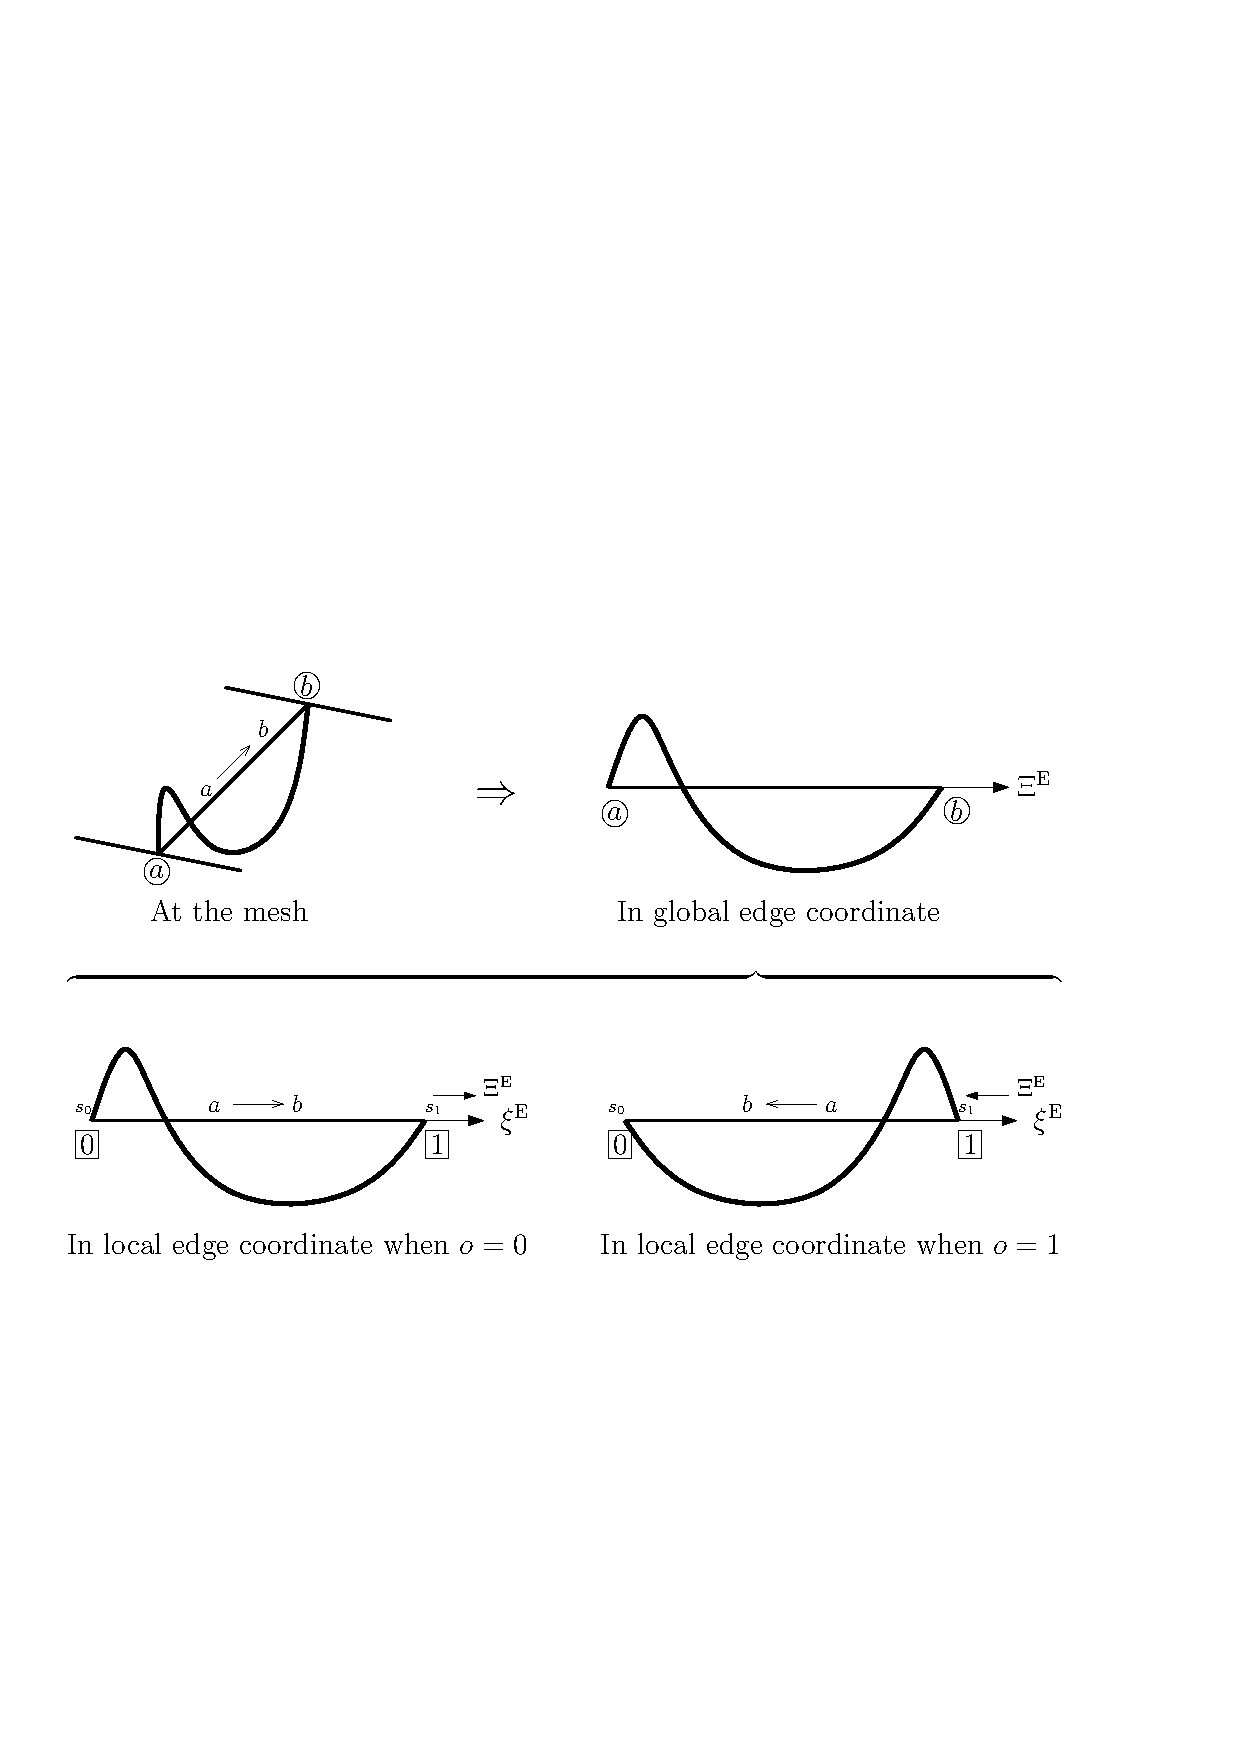
\includegraphics[scale=0.75]{./figures/OrientationsEdge.pdf}
\caption{Edge orientations.}
\label{fig:orientationsedge}
\end{center}
\end{figure}

%However, as the number of spatial dimensions increase, the trace will involve edge and face values over the elements.
%These \textit{do} have a concept of orientation.
%This makes the process of ``matching'' the trace of adjacent shape functions considerably more difficult.
In 2D, if one naively disregards how the elements are placed in the global mesh, and proceeds to define all shape functions at the (local) master element level, one might end up with shape functions that, when transformed back into the original mesh, are incompatible across shared edges (see Figure \ref{fig:edgemismatchintro}).
With orientation embedded shape functions this problem is avoided by taking into account more information of the global mesh. %when defining shape functions at the (local) master element.
This is done by giving each mesh edge its own \textit{global orientation}, and is represented by a global coordinate $\Xi^\E$, or equivalently by a \textit{global edge vertex-ordering}.
For example, given an edge at the mesh with vertices $a$ and $b$, a global edge vertex-ordering of the form $a\tto b$ means that $\Xi^\E$ has its origin at $a$ and points from $a$ to $b$.
This information is then passed to the particular master element, where the edge has its own fixed \textit{local orientation}, represented by the local coordinate $\xi^\E$, or equivalently by the the fixed \textit{local} edge vertex-ordering of the form $\boxednum{0}\!\tdashto\boxednum{1}$ (note the dashed arrow for \textit{local} orderings).
Viewed at the local level, the global coordinate $\Xi^\E$ can either coincide with the local coordinate $\xi^\E$ or point in the opposite direction.
To reflect these \textit{two} possibilities, the orientation parameter $\oo$ is introduced.
If $\oo=0$, this means the local and global coordinates coincide, and otherwise $\oo=1$.
%Notice that the global coordinate $\Xi^{\mathrm{e}}$ can be represented by the ordering of the vertices of the edge in the global mesh. This is referred to as the \textit{edge vertex-ordering}.
All this is depicted in Figure \ref{fig:orientationsedge}. % where the global orientation of the edge with vertices $a$ and $b$ is represented by the edge vertex-ordering $a\to b$, meaning that $\Xi^{\mathrm{e}}$ has its origin at $a$ and points from $a$ to $b$.
%This is shown in Figure \ref{fig:edgemismatch}.

%\begin{figure}[!ht]
%\begin{center}
%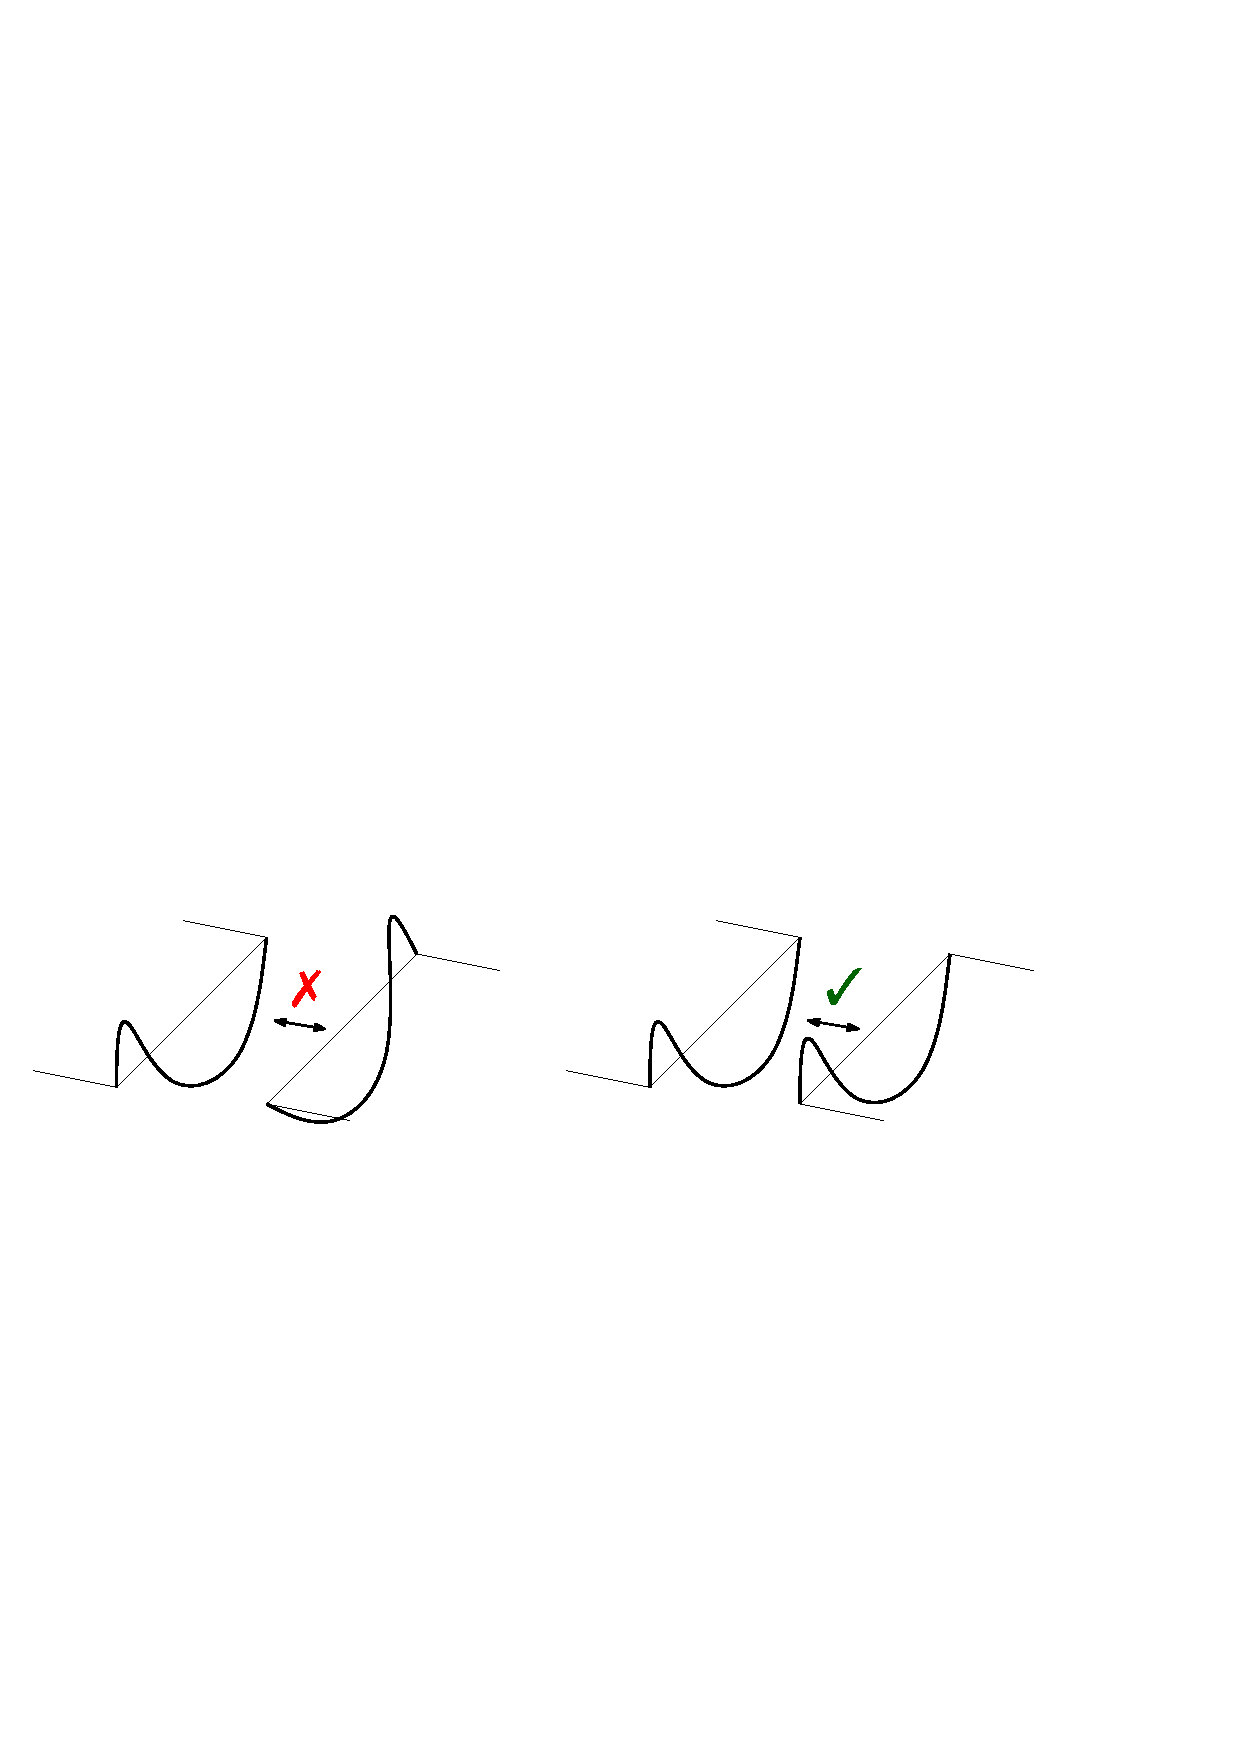
\includegraphics[scale=0.7]{./figures/OrientationsEdgeMismatch.pdf}
%\caption{Potential edge function mismatch in 2D due to disregarding the global mesh.}
%\label{fig:edgemismatch}
%\end{center}
%\end{figure}

%There are different ways to handle this issue.
%Traditionally it is done at the finite element assembly level.
%However, another practical alternative in many cases is to handle the problem at a much earlier point.
%This approach is called \textit{orientation embedding}.
%It consists of fixing or embedding an ``orientation'' to each relevant topological entity when the mesh is initially specified.

%For example, given a mesh in two dimensions, each edge is given its own ``orientation'', which corresponds to fixing a \textit{global edge axis} to each edge. It will be denoted by .
%In addition to this axis, there is a \textit{predefined local edge axis} for each edge at the master element level, denoted by $\xi^\mathrm{e}$.
%The edge shape function will have a fixed form when viewed from the global edge axis.
%Unfortunately, the shape function needs to be expressed in local axis coordinates, because these are associated to the master element and in turn to the integration procedure.
%Clearly the global edge axis only has two possibilities: it is either aligned with the local edge axis or it is not aligned.
%This is expressed by the orientation parameter $\oo$.
%If $\oo=0$ then the two axes are aligned, and if $\oo=1$ the two axes are not aligned. See Fig. (\textit{figure on orientation})

%The \textit{orientation embedded} shape functions are then constructed taking the extra orientation parameter $\oo$ into account.
%Note that shape functions are expressed in terms of master element coordinates, so the global orientation affects not only the function itself, but the derivative as well.

Due to the use of affine coordinates and the form of the ancillary functions proposed in this work, these orientation problems can be readily tackled.
To ensure full compatibility, we want the shape functions over a given edge to be immovable when observed in the global coordinates (like in Figure \ref{fig:orientationsedge}).
This is achieved by evaluating the ancillary functions with global coordinates.
Unfortunately, the available coordinates produced by the master element are the (fixed) local coordinates.
Hence, the idea is to apply a \textit{local-to-global transformation} over the edge, which will obviously depend on the orientation parameter $\oo$. 
Such a transformation is completely natural in the context of affine coordinates, since this only involves permutations of these coordinates.
Indeed, a simple permutation function dependent on $\oo$, denoted by $\sigma_\oo^\E$, will represent this transformation.

\begin{definition*}
Let $s_0$ and $s_1$ be arbitrary variables, and let $\oo=0,1$ be the edge orientation parameter. 
The edge orientation permutation function, $\sigma_\oo^\E$, is defined as
\begin{equation}
	\sigma_\oo^\E(s_0,s_1)=\begin{cases}\sigma_0^\E(s_0,s_1)=(s_0,s_1)&\quad\text{if  }\,\oo=0\,,\\
		\sigma_1^\E(s_0,s_1)=(s_1,s_0)&\quad\text{if  }\,\oo=1\,.\end{cases}\label{eq:orientEdge}
\end{equation}
\end{definition*}

%As expected, when $\oo=0$, there should be no changes, and this is reflected by $\sigma_\oo^\E$.
To explain the definition of $\sigma_\oo^\E$, note that in \eqref{eq:orientEdge}, if one links $s_0$ to the local vertex $\boxednum{0}$ and $s_1$ to the local vertex $\boxednum{1}$, then the \textit{locally ordered} pair $(s_0,s_1)$ represents the local coordinates.
It is ordered in the sense that $s_0$ comes first and $s_1$ comes second, and this is meant to correspond with the fixed \textit{local} ordering $\boxednum{0}\!\tdashto\boxednum{1}$, where $\boxednum{0}$ comes first and $\boxednum{1}$ comes second.
%It is ordered in the sense that just like in the fixed local ordering $\boxednum{0}\!\to\!\boxednum{1}\,$, first comes $\boxednum{0}$ and second comes $\boxednum{1}$, for the affine coordinates (the variables) first comes $s_0$ and second comes $s_1$.
Similarly, there are \textit{globally ordered} pairs which depend on the parameter $\oo$.
Indeed, in Figure \ref{fig:orientationsedge}, looking at the \textit{global} edge vertex-ordering $a\tto b$, there is an induced \textit{global} vertex-ordering of the two vertices $\boxednum{0}$ and $\boxednum{1}$.
It is $\boxednum{0}\!\tto\boxednum{1}$ if $\oo=0$, and $\boxednum{1}\!\tto\boxednum{0}$ if $\oo=1$.
Hence, the global coordinates are represented by the globally ordered pairs $(s_0,s_1)$ if $\oo=0$ and $(s_1,s_0)$ if $\oo=1$.
Therefore, in this sense, $\sigma_\oo^\E$ is a local-to-global transformation.

Now, all that is required is to compose the \textit{edge} ancillary functions and their differential form (those with superscript $\e$) with this permutation function $\sigma_\oo^\E$.
Thus, in 2D and 3D, all instances of $\phi_i^\E$ and $\nabla\phi_i^\E$ in the shape functions should be replaced with $\phi_i^\E\circ\sigma_\oo^\E$ and $\nabla\phi_i^\E\circ\sigma_\oo^\E$ respectively.
The resulting functions are then said to be \textit{orientation embedded} shape functions.
More concrete examples will be given in the 2D and 3D elements as the document progresses.


% the orientation $\oo$. Denoted by $\phi_i^{\e,\oo}$, the orientated ancillary function will be defined by permutations of the entries of the original function $\phi^\E_i$.
%Naturally, when $\oo=0$, the arguments of $\phi^\E_i$ are not permuted, while if $\oo=1$, the arguments are permuted.
%More explicitly,
%\begin{equation}
%    \phi_i^{\e,\oo}(s_0,s_1)=\begin{cases}\phi_i^{\e,0}(s_0,s_1)=\phi_i^{\e}(s_0,s_1)&\quad\text{if  }\,\oo=0\\
%        \phi_i^{\e,1}(s_0,s_1)=\phi_i^{\e}(s_1,s_0)&\quad\text{if  }\,\oo=1\,,\end{cases}\label{eq:edgeorientations}
%\end{equation}
%where $i=2,\ldots,p_s$. The same orientation rule applies for the derivatives and more generally to any function defined from now on which has a superscript $\e$.

%\begin{figure}[ht!]
%\centering
%%\includegraphics[width=\textwidth]{./figures/orientation.png}
%\caption{Two natural orientations of $E$.}
%\label{fig:EdgeOrientations}
%\end{figure}

%Given the functions $\mu_n$, $n=0,1$, defined in Equation~\eqref{eq:H1_1DAffine}, note that
%\[
%\mu_0+\mu_1 = 1\,, \quad \text{and}\quad \mu_n \geq 0\,,\, n=0,1
%\]
%at every point in $\e$. Therefore, $\mu_n$ are affine coordinates for $\e$.
%
%% We now concern ourselves with writing our edge functions, $\phi^\mathrm{e}_i$ as functions of affine coordinates.
%With an eye towards the coming  constructions, we define the orientation $\oo=0$ affine $H^1$ edge shape function as the homogenization of the Lobatto polynomials,
%\be
%\phi^\E_i(s_0,s_1) := \left[L_i\right] (s_0,s_1)\, , \quad i=2,\ldots,p\,.
%\label{eq:EdgeShap1}
%\ee
%Here, $s_0,\,s_0$, are arbitrary variables.
%Recalling the constraint $\mu_0+\mu_1=1$, we can reduce the equation above to,
%\be
%\phi^\E_i(\mu_0,\mu_1) = \left[L_i\right] (\mu_0,\mu_1) = L_i(\mu_1;\mu_0+\mu_1) = L_i(\mu_1),
%\ee
%when its arguments are affine functions of $\e$.
%
%Observe that orientation changes of the affine $H^1$ edge shape functions can be accounted for simply by permuting the ordering of the arguments in Equation~\eqref{eq:EdgeShap1} (see Figure~\ref{fig:EdgeOrientations})
%\be
%\phi^{\e,\oo}_i(\mu_0,\mu_1) =
%\left\{
%    \begin{array}{ll}
%        \left[L_i\right](\mu_0,\mu_1) = L_i(\mu_1) & \text{if } \oo = 0\\
%        \left[L_i\right](\mu_1,\mu_0) = L_i(\mu_0) & \text{if } \oo = 1
%    \end{array}
%\right.\,.
%\label{eq:1DOrientedAffineEdge}
%\ee
%
%Finally, we redefine the $1$D edge bubbles (with orientation accounted for) as
%\be
%\phi^\mathrm{e}_i(\xi) = \phi^{\e,\oo}_i(\mu_0(\xi),\mu_1(\xi))\,.
%\ee
%
%\paragraph*{Generalizations.}
%Here, we revisit Equation~\eqref{eq:EdgeShap1} to produce two general formulas which will arise in many shape functions constructions throughout the rest of the text.
%
%% \begin{remark}
%% We will see later the function $\phi^\E_i$ arise in many shape functions constructions. In other contexts,
%We will often find
%it necessary to consider the spatial gradient of $\phi^\E_i(s_0,s_1)$ where $s_n$, $n=0,1$, are functions of some spatial variable, $\xi$. We present the following general formula for future reference
%\begin{align}
%\bfnab_\xi \phi^\E_i\left(s_0,s_1\right) &= \bfnab_\xi L_i\left(s_1;s_0+s_1\right)
%\nonumber\\
%&= \frac{\ptl L_i}{\ptl x}\left(s_1;s_0+s_1\right) \bfnab_\xi s_1 + \frac{\ptl L_i}{\ptl t}\left(s_1;s_0+s_1\right) \bfnab_\xi\left(s_0+s_1\right)
%\nonumber\\
%% &= P_i\left(s_1(\xi);s_0(\xi)+s_1(\xi)\right) \bfnab_\xi s_1(\xi) + \frac{\ptl L_i}{\ptl t}\left(s_1(\xi);s_0(\xi)+s_1(\xi)\right) \bfnab_\xi\left(s_0(\xi)+s_1(\xi)\right)
%% \\
%&= \left[P_{i-1}\right]\left(s_0,s_1\right) \bfnab_\xi s_1 + \left[R_{i-1}\right]\left(s_0,s_1\right) \bfnab_\xi\left(s_0+s_1\right)\,.
%\label{eq:AffineEdgeGradient}
%\end{align}
%
%Moreover, we define the general, oriented, affine edge shape functions
%\be
%\phi^{\e,\oo}_i(s_0,s_1) =
%\left\{
%    \begin{array}{ll}
%        \left[L_i\right](s_0,s_1) & \text{if } \oo = 0\\
%        \left[L_i\right](s_1,s_0) & \text{if } \oo = 1
%    \end{array}
%\right.\,.
%\label{eq:OrientedAffineEdge}
%\ee
%Agreement of Equation~\eqref{eq:OrientedAffineEdge} with Equation~\eqref{eq:1DOrientedAffineEdge} is immediate.
%


% \end{remark}

% \begin{remark}
% Note that function $\phi_i$ in Equation~\eqref{eq:EdgeShap1} is not unique, but since each $\left[\phi_i\right]$ belong to the same equivalence class, the construction of the edge shape function, as a function of $\xi$ will be independent of the choice of $\phi_i$.
% \end{remark}

%Section 4
\newpage
\section{Quadrilateral}
\label{sec:Quad}

\begin{figure}[!ht]
\begin{center}
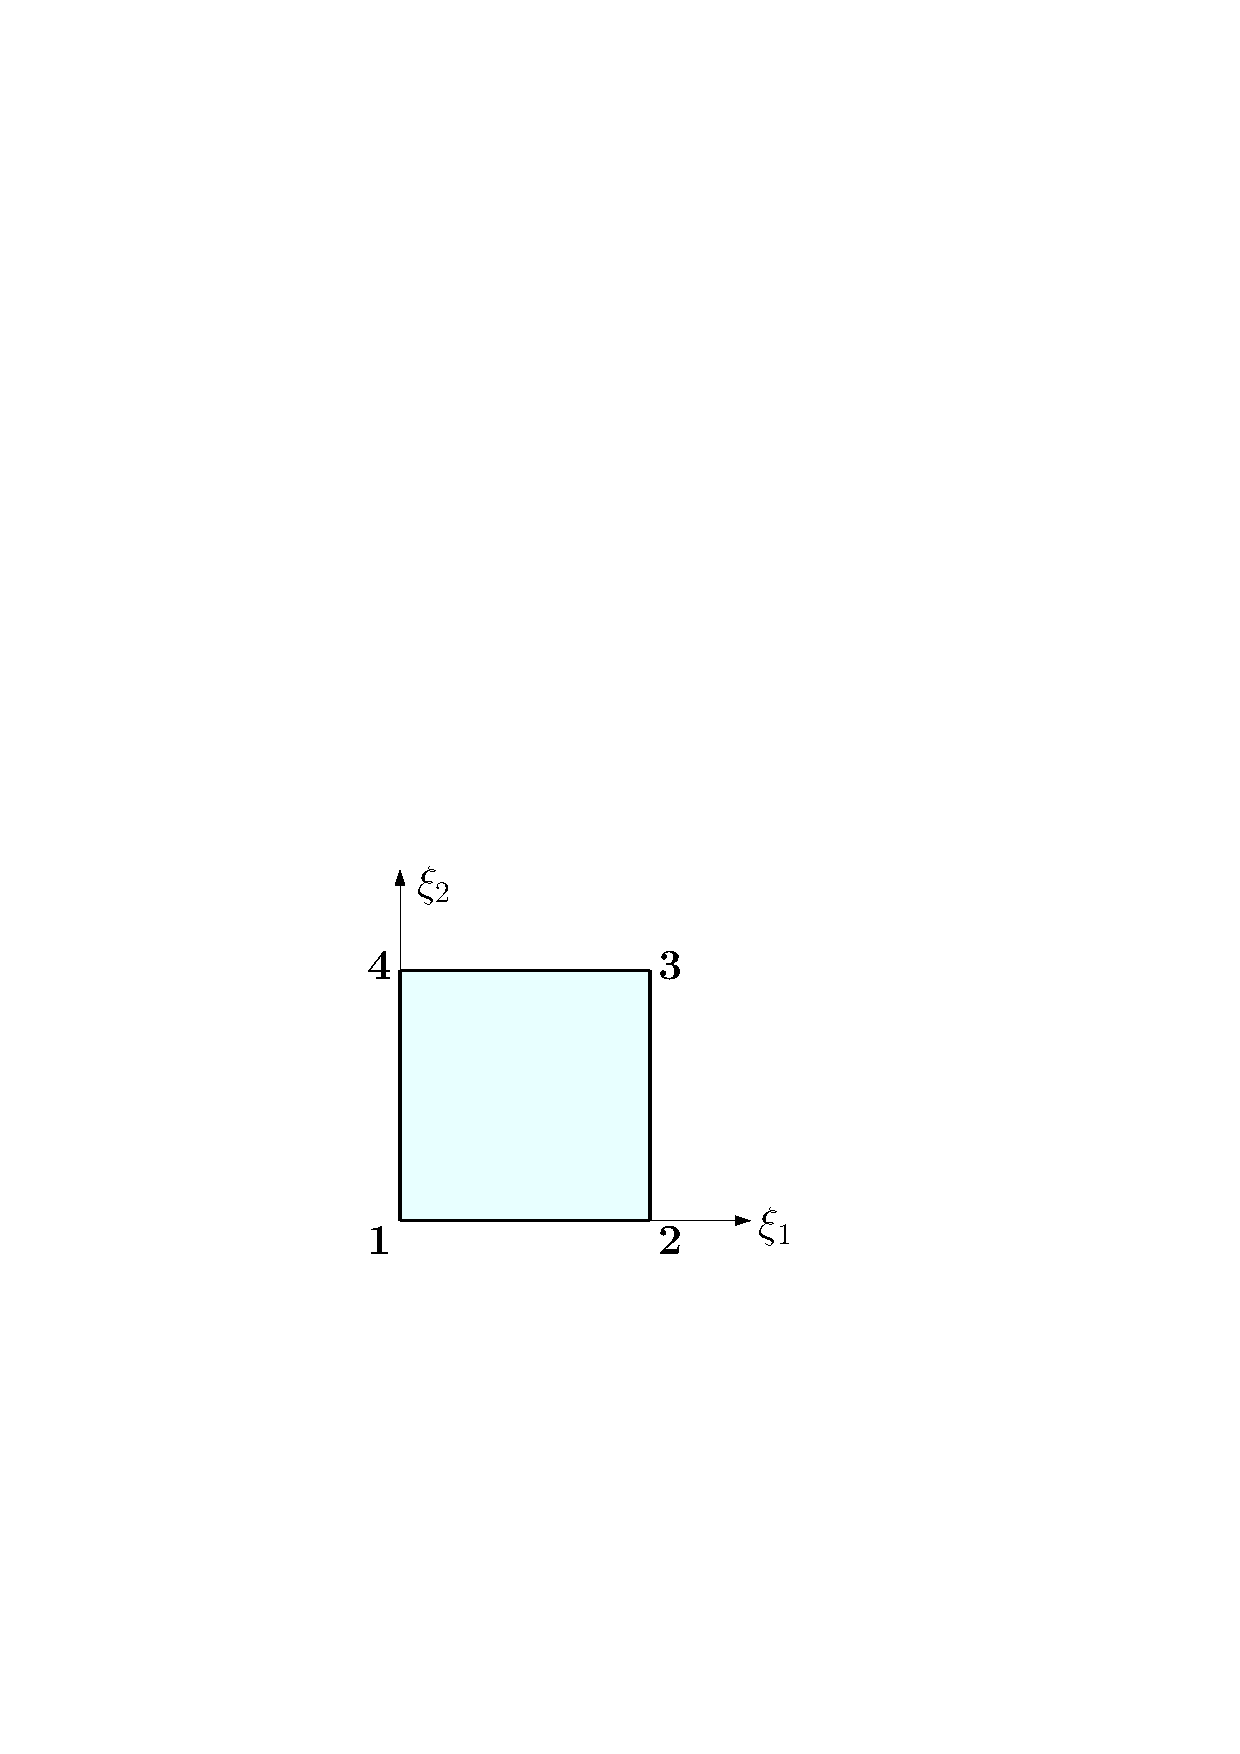
\includegraphics[scale=0.5]{./figures/MasterQuad.pdf}
\caption{Master quadrilateral with numbered vertices.}
\label{fig:MasterQuad}
\end{center}
\end{figure}

The master element for quadrilaterals, which is $(0,1)^2$, is shown in Figure \ref{fig:MasterQuad} in $\xi=(\xi_1,\xi_2)$ space.
The master quadrilateral is clearly a Cartesian product of two segments.

Due to the product structure, there are \textit{two} pairs of 1D affine coordinates:
\begin{equation}
    \begin{alignedat}{4}
        \mu_0(\xi_1)&=1-\xi_1\,,\quad \mu_1(\xi_1)=\xi_1\,\qquad&\Rightarrow\qquad
            \nabla\mu_0(\xi_1)&=\Big(\begin{smallmatrix}-1\\[2pt]0\end{smallmatrix}\Big)\,,\quad
                \nabla\mu_1(\xi_1)=\Big(\begin{smallmatrix}1\\[2pt]0\end{smallmatrix}\Big)\,,\\
        \mu_0(\xi_2)&=1-\xi_2\,,\quad \mu_1(\xi_2)=\xi_2\,\qquad&\Rightarrow\qquad
            \nabla\mu_0(\xi_2)&=\Big(\begin{smallmatrix}0\\[2pt]-1\end{smallmatrix}\Big)\,,\quad
                \nabla\mu_1(\xi_2)=\Big(\begin{smallmatrix}0\\[2pt]1\end{smallmatrix}\Big)\,.
    \end{alignedat}
\end{equation}
These will be used explicitly or implicitly in the formulas that follow.

Again, vertex $a$ is denoted by $v_a$, so that $v_1=(0,0)$, $v_2=(1,0)$, $v_3=(1,1)$ and $v_4=(0,1)$.
These vertices are related to the affine coordinates just as in 1D.
For example, over edge 12 (or edge 43), $\mu_0(\xi_1)$ is the weight related to $v_1$, while $\mu_1(\xi_1)$ is the weight related to $v_2$ (and similarly with $v_4$ and $v_3$).
Indeed, given a point $(\xi_1,0)$ on edge 12, it holds that $(\xi_1,0)=\mu_0(\xi_1)v_1+\mu_1(\xi_1)v_2$.
The same way, $\mu_0(\xi_2)$ is related to $v_1$ in edge 14, so that $v_1$ is linked to both $\mu_0(\xi_1)$ and $\mu_0(\xi_2)$.
A similar assertion holds for each vertex, where each is linked to \textit{two} affine coordinates.
Now, looking at the edges, note that $\mu_0(\xi_2)$ takes the value $1$ over edge 12 and $0$ at opposite edge 43.
This way, each edge is linked to \textit{one} affine coordinate.

\subsubsection*{Exact Sequence}
% The two dimensional exact sequence is of the form
% \begin{equation}
% H^1 \xrightarrow{\,\,\nabla\,\,} H(\mathrm{curl}) \xrightarrow{\nabla\times} L^2 \,,
% \label{eq:2DExactSeq}
% \end{equation}
% where $\nabla\times$ is understood in two dimensions:
% \begin{equation}
%     \nabla\times E=\nabla\times\begin{pmatrix}E_1\\E_2\end{pmatrix}
%         =\frac{\partial E_2}{\partial \xi_1}-\frac{\partial E_1}{\partial \xi_2}\,,\qquad\quad
%     E\times F=\begin{pmatrix}E_1\\E_2\end{pmatrix}\times\begin{pmatrix}F_1\\F_2\end{pmatrix}
%         =E_1 F_2 - E_2 F_1\,.
% \end{equation}
% By ``rotating'' $H(\mathrm{curl})$, the space $H(\mathrm{div})$ arises naturally:
% \begin{equation}
%     H(\mathrm{div})=\Big\{V_E=\Big(\begin{smallmatrix}0&1\\-1&0\end{smallmatrix}\Big)E=
%         \Big(\begin{smallmatrix}E_2\\-E_1\end{smallmatrix}\Big):
%             E=\Big(\begin{smallmatrix}E_1\\E_2\end{smallmatrix}\Big)\in H(\mathrm{curl})\Big\}\,,\label{eq:Hdiv2Ddef}
% \end{equation}
% Defined in this way, the ``rotated'' exact sequence is immediately satisfied:
% \begin{equation}
% H^1 \xrightarrow{\mathrm{curl}} H(\mathrm{div}) \xrightarrow{\nabla\cdot} L^2 \,,
% \label{eq:2DExactSeqRotated}
% \end{equation}
% where the operations satisfy the following relations:%$\mathrm{curl}\,(\phi)$ is understood as
% \begin{equation}
%     \mathrm{curl}\,(\phi):=\begin{pmatrix}\frac{\partial\phi}{\partial \xi_2}\\[4pt]-\frac{\partial\phi}{\partial \xi_1}\end{pmatrix}
%         =\begin{pmatrix}0&1\\[4pt]-1&0\end{pmatrix}\nabla\phi\,,\qquad\quad
%             \nabla\cdot V_E=\nabla\cdot\begin{pmatrix}0&1\\[4pt]-1&0\end{pmatrix}E=\nabla\times E\,,
% \end{equation}
% for all $\phi\in H^1$ and all $E\in H(\mathrm{curl})$.

Recall the 2D exact sequence for simply connected domains \eqref{eq:2DExactSeq} and its rotated analogue \eqref{eq:2DExactSeqRotated}.
%\begin{equation}
%\begin{alignedat}{4}
%	&H^1 \xrightarrow{\,\,\nabla\,\,} &&H(\mathrm{curl}) \xrightarrow{\nabla\times} \,&L^2 \,,\\
%	&H^1 \xrightarrow{\mathrm{curl}\,}\, &&H(\mathrm{div})\, \xrightarrow{\,\,\nabla\cdot\,\,} &L^2 \,.
%\end{alignedat}
%\end{equation}
The corresponding polynomial exact sequences are
\begin{equation}
	\begin{alignedat}{4}
    &\mathcal{Q}^{p,q} \xrightarrow{\,\,\nabla\,\,} & \mathcal{Q}^{p-1,q}\times\mathcal{Q}^{p,q-1} 
    	\xrightarrow{\nabla\times} &&\mathcal{Q}^{p-1,q-1} \,,\\
    &\mathcal{Q}^{p,q} \xrightarrow{\mathrm{curl}\,} &\mathcal{Q}^{p,q-1}\times\mathcal{Q}^{p-1,q} 
    	\xrightarrow{\,\nabla\cdot\,} &&\mathcal{Q}^{p-1,q-1} \,,
	\end{alignedat}
	\label{eq:QuadES}
\end{equation}
where $\mathcal{Q}^{p,q}=\mathcal{Q}^{p,q}(\xi_1,\xi_2)=\mathcal{P}^p(\xi_1)\otimes\mathcal{P}^q(\xi_2)$. 
These are the standard N\'{e}d\'{e}lec's spaces \citeyearpar{Nedelec80} of the first type for the quadrilateral.
%are utilized:
%\begin{equation}
%    \begin{aligned}
%    W^{p,q} & = \mathcal{Q}^{p,q}= \mathcal{P}^p(\xi_1)\otimes \mathcal{P}^q(\xi_2)\,, \\
%    Q^{p,q} & = \mathcal{Q}^{p-1,q} \times\mathcal{Q}^{p,q-1}\,, \\
%    V^{p,q} & = \mathcal{Q}^{p,q-1} \times\mathcal{Q}^{p-1,q}\,, \\
%    Y^{p,q} & = \mathcal{Q}^{p-1,q-1}\,.
%    \end{aligned}
%\end{equation}
Note here the natural anisotropy of the element, which has order $p$ in the $\xi_1$ direction and a potentially different $q$ in the $\xi_2$ direction. 
The hierarchy should be maintained in both $p$ and $q$ separately. 
This is associated to the notion of local $p$ adaptivity. 
It will sometimes be convenient to refer to $p_a$ as the order in the $\xi_a$ direction, so that $p_1=p$ and $p_2=q$.
%We follow the construction of Ainsworth and Coyle\cite{AinsworthCoyle01} based on mimicking the structure of \Nedelec's spaces with Legendre and Lobatto (integrated Legendre) polynomials.

\subsection{\texorpdfstring{$H^1$}{H1} Shape Functions}

%Recall that in two dimensions, the trace of $H^1$ functions is the value of the function itself along the boundary.
%Hence, all vertex functions vanish at all nonadjacent edges, and all edge functions should vanish at all other edges (except the edge that the function is describing).
%The bubbles will vanish at all edges.
It will be clear that all shape functions lie in $\mathcal{Q}^{p,q}$ and that they span the space. 
For this, one will only require the linear independence of the shape functions, which will be evident, and a judicious count of them, which will give $(p+1)(q+1)$ (the dimension of $\mathcal{Q}^{p,q}$).

Also, note that due to the Cartesian product structure, there is a natural separation of variables, and one expects the shape functions to be tensor products of the relevant 1D functions for the edges and vertices. 
That is, tensor products of $\mu_a(\xi_b)$ and $\phi_i^\E(\vec{\mu}_{01}(\xi_b))$, for $a=0,1$ and $b=1,2$.
Fortunately, this is the case.

\subsubsection{\texorpdfstring{$H^1$}{H1} Vertices}
\label{sec:H1QuadVertices}

As mentioned before, each vertex is linked with two affine coordinates, and the \textit{associated} vertex function is precisely the tensor product of these two coordinates.
For instance, $v_1$ is linked to $\mu_0(\xi_1)$ and $\mu_0(\xi_2)$, so its associated vertex function is  
\begin{equation*}
	\phi^\mathrm{v}(\xi)=\mu_0(\xi_1)\mu_0(\xi_2)\,.
\end{equation*}
It satisfies all the desired properties, since it vanishes at the disjoint edges 23 and 34, and more importantly, its trace over the adjacent edges is a 1D $H^1$ vertex function associated to the vertex.
For instance, over edge 12, where $\mu_0(\xi_2)=1$, its trace is $\mu_0(\xi_1)$, which is the 1D $H^1$ vertex function associated to $v_1$ over the edge 12.
Finally, the function decays bilinearly and is in the lowest order possible space, $\mathcal{Q}^{1,1}$, so that it respects the hierarchy in both $p$ and $q$.

More generally, the vertex functions and their gradients are,
\begin{equation}
    \phi^\mathrm{v}(\xi)=\mu_a(\xi_1)\mu_b(\xi_2)\,,\quad\qquad
    \nabla\phi^\mathrm{v}(\xi)=\mu_a(\xi_1)\nabla\mu_b(\xi_2)+\mu_b(\xi_2)\nabla\mu_a(\xi_1)\,.\label{eq:H1vertexquad}
\end{equation}
for $a=0,1$ and $b=0,1$.
%Their gradients are
%\begin{equation}
%    
%\end{equation}
There is a total of $4$ vertex functions (one for each vertex). % function for each vertex, giving a total of \textit{four} vertex functions, which lie in $\mathcal{Q}^{1,1}$.

%As mentioned before, each vertex is linked with two affine coordinates, and the \textit{associated} vertex function is precisely the product of these two coordinates.
%For instance, $v_1$ is linked to $\mu_0(\xi_1)$ and $\mu_0(\xi_2)$, so it is associated to the vertex function $\phi^\mathrm{v}(\xi)=\mu_0(\xi_1)\mu_0(\xi_2)$, where $a=0$ and $b=0$ in \eqref{eq:H1vertexquad}.
%Each function takes the value $1$ at $(a,b)$ and $0$ at all the other vertices, as required.
%This means the vertex with coordinates $(a,b)$ is correlated with the vertex function $\mu_a(\xi_1)\mu_b(\xi_2)$, so that in fact it is related to the 1D affine coordinates $\mu_a(\xi_1)$ and $\mu_b(\xi_2)$.
%For example, vertex 1, which has coordinates $(0,0)$, is associated to $\mu_0(\xi_1)$ and $\mu_0(\xi_2)$ and so on.

%Moreover, the vertex blending across both edges is linear, since the trace over the edges is always of the form $\mu_a(\xi_b)$ for $a=0,1$ and $b=1,2$.
%This makes the vertex shape functions compatible in 2D with neighboring quadrilateral vertex functions (see Figure \ref{fig:2Dvertexcompatibility} in \S\ref{sec:compatibility}).
%They will be compatible with triangles as well if the vertex blending across the edges for the triangle vertex functions is also linear.
%Notice the shape functions \textit{have} to be in $\mathcal{Q}^{1,1}$ to enforce hierarchy (if this is a desired aspect in the construction), since anything else within $\mathcal{Q}^{p,q}$ would destroy the hierarchy in either $p$ or $q$.

%Note the blending across the face (basically the function itself) presents a bilinear decay. 
%Just like the traces over the edges of these 2D vertex functions were precisely the 1D vertex functionsAs a preview to the higher dimensional elements, note that 

%Clearly, as required, they vanish at all vertices except the one with coordinates $(a,b)$.
%By linearity this means they also vanish at all nonadjacent edges.
%Moreover, their traces over adjacent edges are of the form $\mu_b(\xi_a)$ for some $a=1,2$ and $b=0,1$, which coincides with the segment case.
%This makes the traces compatible with any potential neighboring element.
%
%From now on, $p_a$ is the order in the $\xi_a$ axis, so that $p_1=p$ and $p_2=q$.

\subsubsection{\texorpdfstring{$H^1$}{H1} Edges}
\label{sec:H1edgesQuad}
To ease the comprehension, take for example edge 12, where $\xi_2=0$.
The idea for the edge functions is to use the segment bubbles $\phi_i^\E$ in $\xi_1$ and \textit{blend} them with a linear function in $\xi_2$.
That is, blend them with the linked 1D affine coordinate, $\mu_0(\xi_2)$.
Hence, the associated edge functions will be the tensor products of $\phi_i^\E(\vec{\mu}_{01}(\xi_1))$ and $\mu_0(\xi_2)$,
\begin{equation*}
    \phi_i^\mathrm{e}(\xi)=\mu_0(\xi_2)\phi_i^\E(\vec{\mu}_{01}(\xi_1))=(1-\xi_2)L_i(\xi_1)\,,
\end{equation*}
with $i=2,\ldots,p$.
The trace properties are satisfied mainly due to the vanishing conditions of the $L_i$ at the endpoints (see \eqref{eq:Lvanishatendpoints}), which are restated in terms of $\phi_i^\E$ in \eqref{eq:phiEvanishing}. 
The vanishing properties are easily observed in the simplified form, $(1-\xi_2)L_i(\xi_1)$, but we will write these traces in terms of the ancillary functions and the affine coordinates. %since this type of analysis extrapolates more naturally to the other elements.
%For this, note the edge traces can be written in terms of affine coordinates, since 
For this, it is useful to write the boundary restrictions in terms of affine coordinates.
For example, over edge 12, which has equation $\xi_2=0$, $\vec{\mu}_{01}(\xi_2)=(\mu_0(\xi_2),\mu_1(\xi_2))=(1,0)$. 
%Using these natural relationships between the traces and affine coordinates, the traces over the edges are
Using these natural relationships, the edge traces are
\begin{align*}
    \phi_i^\mathrm{e}(\xi)|_{\xi_2=0}&=\mu_0(\xi_2)\phi_i^\E(\vec{\mu}_{01}(\xi_1))|_{\vec{\mu}_{01}(\xi_2)=(1,0)}
    	=1\cdot\phi_i^\E(\vec{\mu}_{01}(\xi_1))=\phi_i^\E(\vec{\mu}_{01}(\xi_1))\,,\\
    \phi_i^\mathrm{e}(\xi)|_{\xi_1=1}&=\mu_0(\xi_2)\phi_i^\E(\vec{\mu}_{01}(\xi_1))|_{\vec{\mu}_{01}(\xi_1)=(0,1)}
    	=\mu_0(\xi_2)\phi_i^\E(0,1)=0\,,\\
  	\phi_i^\mathrm{e}(\xi)|_{\xi_2=1}&=\mu_0(\xi_2)\phi_i^\E(\vec{\mu}_{01}(\xi_1))|_{\vec{\mu}_{01}(\xi_2)=(0,1)}
    	=0\cdot\phi_i^\E(\vec{\mu}_{01}(\xi_1))=0\,,\\
    \phi_i^\mathrm{e}(\xi)|_{\xi_1=0}&=\mu_0(\xi_2)\phi_i^\E(\vec{\mu}_{01}(\xi_1))|_{\vec{\mu}_{01}(\xi_1)=(1,0)}
    	=\mu_0(\xi_2)\phi_i^\E(1,0)=0\,.
\end{align*}
%At a more general level, these conditions are simply inherited from the vanishing conditions of each of the components of the tensor product structure, $\phi_i^\E(\vec{\mu}_{01}(\xi_1))$ and $\mu_0(\xi_2)$.
%That is, note that over edges 14 and 23, $\mu_0(\xi_1)=0$ and $\mu_1(\xi_1)=0$ respectively, so that by \eqref{eq:phiEvanishing}, $\phi_i^\E(\vec{\mu}_{01}(\xi_1))=0$ in both cases.
%Then, over edge 34, $\mu_0(\xi_2)=0$.
Hence, the desired vanishing properties are satisfied, and more importantly, over the edge 12 itself, the trace is $\phi_i^\E(\vec{\mu}_{01}(\xi_1))$ which as expected is a 1D $H^1$ edge bubble.
%This will make it compatible with neighboring edge functions (see Figure \ref{fig:2Dedgecompatibility} in \S\ref{sec:compatibility}).
Note here the decay towards the rest of the element, represented by the blending function $\mu_0(\xi_2)$, is linear.
Indeed, the edge functions for edge 12 lie in $\mathcal{Q}^{p,1}$ and they respect the hierarchy in $q$.
%This does not affect compatibility in 2D, but it must be linear to enforce the hierarchy in $q$ (the $\xi_2$ direction).
%Note that on edge 12 it collapses to $\phi_i^\E(\mu_0(\xi_1),\mu_0(\xi_1))=L_i(\xi_1)$ which is precisely what is desired, since it will have the same form as edges of adjacent elements.

Next, we will give a geometrical representation of the edge 12 shape functions presented above.
Recall that over edge 12, $v_1$ is linked to $\mu_0(\xi_1)$, while $v_2$ is linked to $\mu_1(\xi_1)$. 
Hence, $\vec{\mu}_{01}(\xi_1)=(\mu_0(\xi_1),\mu_1(\xi_1))$ actually represents a point in the edge,
%First, remember from the vertex functions that each vertex is associated to two 1D affine coordinates.
%For edge 12, vertex 1, $v_1=(0,0)$, is related to $\mu_0(\xi_1)$, while vertex 2, $v_2=(1,0)$ is related to $\mu_1(\xi_1)$ (and both are associated to $\mu_0(\xi_2)$)
%Then, recall the affine coordinates actually represent a point over the given simplex, so that $\vec{\mu}_{01}(\xi_1)$ represents some point over edge 12. 
%Indeed, by \eqref{eq:affinerepresentation},
\begin{equation*}
	\mu_0(\xi_1)\Big(\begin{smallmatrix}0\\[2pt]0\end{smallmatrix}\Big)
		+\mu_1(\xi_1)\Big(\begin{smallmatrix}1\\[2pt]0\end{smallmatrix}\Big)
			=\Big(\begin{smallmatrix}\xi_1\\[2pt]0\end{smallmatrix}\Big)\,.
\end{equation*} 
This can be interpreted as a projection to edge 12 from an arbitrary point $(\xi_1,\xi_2)$,
\begin{equation*}
    (\xi_1,\xi_2)\;\longmapsto\;(\xi_1,0)\,.
\end{equation*}
The trivial projection consists simply of finding the intersection $P'=(\xi_1,0)$ of the edge with the normal projecting line passing through the original point $P=(\xi_1,\xi_2)$. 
It is better illustrated in Figure \ref{fig:QuadProjection}.

\begin{figure}[!ht]
\begin{center}
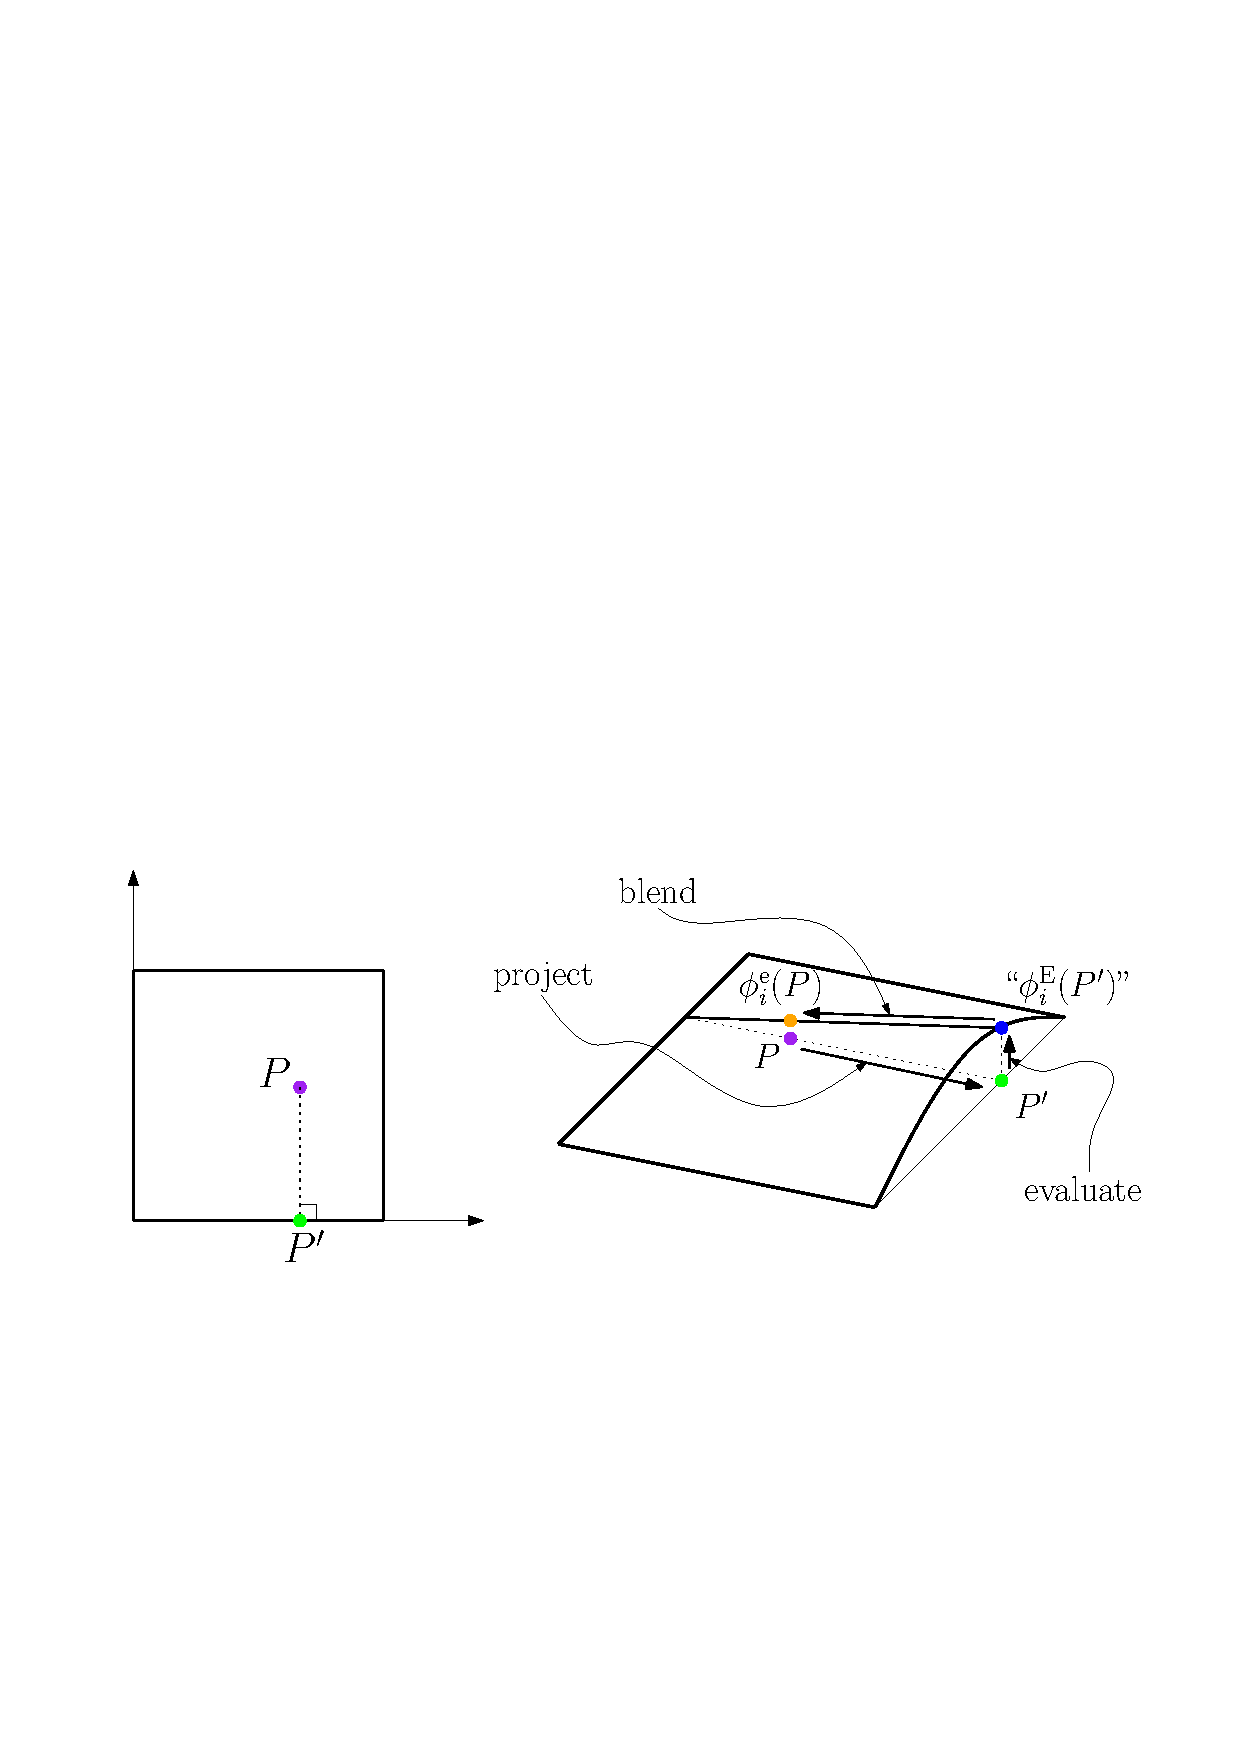
\includegraphics[scale=0.55]{./figures/QuadProjection.pdf}
\caption{Edge projection from $P$ to $P'$, and the logic project$\,\to\,$evaluate$\,\to\,$blend.}
\label{fig:QuadProjection}
\end{center}
\end{figure}

After the original point is projected to the desired edge, it is evaluated at that edge, and finally it is blended linearly:
\begin{equation*}
    \phi_i^\mathrm{e}(\xi)=\underbrace{\mu_0(\xi_2)}_{\text{blend}}
        \underbrace{\phi_i^\E(\underbrace{\vec{\mu}_{01}(\xi_1)}_{\text{project}})}_{\text{evaluate}}
    	=\underbrace{(1-\xi_2)}_{\text{blend}}\underbrace{L_i(\underbrace{\xi_1}_{\text{project}})}_{\text{evaluate}}\,.
\end{equation*}
This blending represents and extension or lifting to the rest of the element.
The whole process of
\begin{equation*}
	\text{projecting}\longrightarrow\text{evaluating}\longrightarrow\text{blending}
\end{equation*}
is extremely important, since it is used in the construction of shape functions for all remaining elements. 
Moreover, as depicted in Figure \ref{fig:QuadProjection}, it gives a geometrical interpretation to the formulas. 
It should be mentioned that if orientations are to be handled, they are taken care of only at the level of evaluating, where a local-to-global transformation will need to be prepended to the original evaluating procedure.
%preprocessing representing a local-to-global transformation will need to be added. 
Projecting and blending are unaffected by orientations.

The general formula for edge functions is
\begin{equation}
    \phi_i^\mathrm{e}(\xi)=\mu_c(\xi_b)\phi_i^\E(\vec{\mu}_{01}(\xi_a))\,,\quad\qquad
    	\nabla\phi_i^\mathrm{e}(\xi)=\mu_c(\xi_b)\nabla\phi_i^\E(\vec{\mu}_{01}(\xi_a))
        +\phi_i^\E(\vec{\mu}_{01}(\xi_a))\nabla\mu_c(\xi_b)\,,\label{eq:QuadH1Edge}
\end{equation}
where $i=2,\ldots,p_a$, $(a,b)=(1,2),(2,1)$ and $c=0,1$, with $p_a$ being the order in the $\xi_a$ coordinate. 
%Their gradients are
%\begin{equation}
%    \nabla\phi_i^\mathrm{e}(\xi)=\mu_c(\xi_b)\nabla\phi_i^\E(\mu_0(\xi_a),\mu_1(\xi_a))
%        +\phi_i^\E(\mu_0(\xi_a),\mu_1(\xi_a))\nabla\mu_c(\xi_b)\,.
%\end{equation}
For example for edge 12 (linked to $\mu_c(\xi_b)=\mu_0(\xi_2)$), this would correspond to $(a,b)=(1,2)$, $c=0$ and $p_a=p$, for edge 23 (linked to $\mu_1(\xi_1)$) it is $(a,b)=(2,1)$, $c=1$ and $p_a=q$, and so on. 
For each edge there are $p_a-1$ shape functions, leading to a total of $2(p-1)+2(q-1)$ edge shape functions.
%Just like 

%\paragraph{Edge Orientations.}
%To consider orientations, simply take a predefined $\oo=0$ orientation, which is determined only by looking at the master element axes and the predefined local edge axes for each edge, and replace $\phi_i^\E$ by $\phi_i^{\e,\oo}$. 
%For example, for edge 12, the local axis $\xi^\mathrm{e}$ is parallel to the master element axis $\xi_1$ and more importantly, it points in the \textit{same} direction. 
%This means the order of the entries in $\phi_i^{\e,\oo}$ is $(\mu_0(\xi_1),\mu_1(\xi_1))$ (and $\textit{not}$ $(\mu_1(\xi_1),\mu_0(\xi_1))$ which would apply if the master element axis and the local axis point in \textit{different} directions). 
%This defines the $\oo=0$ orientation.
%Hence, for edge 12, \eqref{eq:Quadphigeneral} becomes
%\begin{equation*}
%    \phi_i^\mathrm{e}(\xi)\!=\!\mu_0(\xi_2)\phi_i^{\e,\oo}(\mu_0(\xi_1),\mu_1(\xi_1))
%        \!=\!\!\begin{cases}
%            \mu_0(\xi_2)\phi_i^{\e,0}(\mu_0(\xi_1),\mu_1(\xi_1))\!
%            	=\!\mu_0(\xi_2)\phi_i^{\e}(\mu_0(\xi_1),\mu_1(\xi_1))\,\,\,\text{if }\oo=0\\
%            \mu_0(\xi_2)\phi_i^{\e,1}(\mu_0(\xi_1),\mu_1(\xi_1))\!
%            	=\!\mu_0(\xi_2)\phi_i^{\e}(\mu_1(\xi_1),\mu_0(\xi_1))\,\,\,\text{if }\oo=1\,,
%        \end{cases}
%\end{equation*}
%where \eqref{eq:edgeorientations} was used as the definition of $\phi_i^{\e,\oo}$. 
%The same applies to the gradients, and the other edge functions that follow in $H(\mathrm{curl})$ (which involve $E_i^\E$, to be defined later). 
%
%The predefined local edge axis is defined at the master element level.
%These predefined axes for each master element edge are shown in the Appendix.
%The predefined local axis explained above for edge 12 is actually the one utilized in our implementation.
%Naturally, in a different implementation one could decide to use other predefined local edge axes, and the $\oo=0$ orientation would change accordingly as explained above.
%In future examples we will only mention those predefined local edge axes that were used in our implementation (see Appendix).

\subsubsection{\texorpdfstring{$H^1$}{H1} Face Bubbles}

The quadrilateral face bubbles can be naturally defined as the tensor product of 1D edge bubbles,
\begin{equation*}
    \phi_{ij}^\mathrm{f}(\xi)=\phi_i^\E(\vec{\mu}_{01}(\xi_1))\phi_j^\E(\vec{\mu}_{01}(\xi_2))\,,
\end{equation*}
for $i=2,\ldots,p$ and $j=2,\ldots,q$. 
Using \eqref{eq:phiEvanishing}, it is clear the vanishing conditions over all four edges are satisfied.
%For this, note it is used that $\textit{both}$ functions vanish at both endpoints.
This motivates a more general definition.

\begin{definition*}
Let $(s_0,s_1)$ and $(t_0,t_1)$ be two pairs of coordinates which are arbitrary functions of some spatial variable in $\R^N$, $N=2,3$. Let $p_s$ be the order in the $(s_0,s_1)$ coordinates, and $p_t$ be the order in the $(t_0,t_1)$ coordinates. Then
\begin{equation}
    \phi_{ij}^\square(s_0,s_1,t_0,t_1)=\phi_i^\E(s_0,s_1)\phi_j^\E(t_0,t_1)\,,
\end{equation}
for $i=2,\ldots,p_s$ and $j=2,\ldots,p_t$. The gradients, understood in $\R^N$, are
\begin{equation}
	\begin{aligned}
    \nabla\phi_{ij}^\square(s_0,s_1,t_0,t_1)&=\phi_i^\E(s_0,s_1)\nabla\phi_j^\E(t_0,t_1)+\phi_j^\E(t_0,t_1)\nabla\phi_i^\E(s_0,s_1)\,.
	\end{aligned}
\end{equation}
\end{definition*}

%To lighten notation, sometimes the coordinate pair $(s_0,s_1)$ or more technically $(s_0(\bcdot),s_1(\bcdot))$ with $(\bcdot)\in\R^N$, is simply referred to as $\vec{s}(\bcdot)$. Hence, from now on, $\vec{\mu}(\xi_a)=(\mu_0(\xi_a),\mu_1(\xi_a))$ for $a=1,2$.

Rewritten in terms of $\phi_{ij}^\square$, the general formulas for the bubbles and their gradients are,
\begin{equation}
    \phi_{ij}^\mathrm{f}(\xi)=\phi_{ij}^\square(\vec{\mu}_{01}(\xi_1),\vec{\mu}_{01}(\xi_2))\,,\qquad\quad
        \nabla\phi_{ij}^\mathrm{f}(\xi)=\nabla\phi_{ij}^\square(\vec{\mu}_{01}(\xi_1),\vec{\mu}_{01}(\xi_2))\,,
\end{equation}
where $i=2,\ldots,p$ and $j=2,\ldots,q$. 
There are a total of $(p-1)(q-1)$ such functions. 
%They are referred to as \textit{the} 2D $H^1$ quadrilateral face bubbles.

\subsection{\texorpdfstring{$H(\mathrm{curl})$}{Hcurl} Shape Functions}
%As a reminder, in two dimensions, the trace of $H(\mathrm{curl})$ functions is the tangential component of the vector function along the boundary (that is, the edges).
%Hence, all edge functions should have vanishing trace at all other edges, while the bubbles should have zero trace at all edges. 
It will be clear that all shape functions will lie in $\mathcal{Q}^{p-1,q}\times\mathcal{Q}^{p,q-1}$. 
Moreover, after all functions are defined, a rigorous count will give $p(q+1)+(p+1)q$, which is precisely the dimension of $\mathcal{Q}^{p-1,q} \times\mathcal{Q}^{p,q-1}$, so that the shape functions span the desired space.
%That is, the shape functions will span precisely $\mathcal{Q}^{p-1,q} \times\mathcal{Q}^{p,q-1}$, as desired.

\subsubsection{\texorpdfstring{$H(\mathrm{curl})$}{Hcurl} Edges}
\label{sec:HcurledgesQuad}
%To begin to understand what is required of $H(\mathrm{curl})$ edge functions, the first important fact to highlight is that at the level of traces the exact sequence is also satisfied for edges (which are one dimensional segments).
%More precisely, the two dimensional edge functions in $H^1$ should have traces in the on dimensional $H^1(\e)$, while the the two dimensional edge functions in $H(\mathrm{curl})$ should have trace in $L^2(\e)$.
%The following diagram gives a better illustration:
%\begin{displaymath}
%    %\text{2D:}&\qquad H^1 \xrightarrow{\,\,\nabla\,\,} H(\mathrm{curl}) \xrightarrow{\nabla\times} L^2 \\
%    %\text{1D:}&\qquad H^1 \xrightarrow{\,\,\nabla\,\,} L^2\,.
%    \xymatrix{
%        {\text{2D:}} & H^1 \ar[r]^{\nabla\,\,\,\,} \ar[d]^{\mathrm{tr}} & H(\mathrm{curl})
%            \ar[r]^{\,\,\nabla\times} \ar[d]^{\mathrm{tr}} & L^2\\
%        {\text{1D:}} & H^1 \ar[r]^{\nabla\,\,\,\,} & \,\,\,\,L^2\,\, }
%\end{displaymath}
%This should be satisfied at the level of polynomial spaces as well.

First, take for instance edge 12.
As mentioned in \S\ref{sec:dimensionalhierarchy}, the tangential trace of the $H(\mathrm{curl})$ edge functions should be a 1D $L^2$ shape function.
%will take the form of one of \textit{the} 1D $L^2$ edge functions over the tangential trace.
From \eqref{eq:the1DL2edge}, the 1D $L^2$ edge functions (with coordinate $\xi_1$) are $[P_i](\vec{\mu}_{01}(\xi_1))$.
Meanwhile, note the tangential vector to edge 12 is $(1,0)=\nabla\mu_1(\xi_1)$.
When coupled with a blending factor, $\mu_0(\xi_2)$, representing a linear decay (like that of $H^1$), this suggests,
\begin{equation*}
    E_i^\mathrm{e}(\xi)=\mu_0(\xi_2)[P_i](\vec{\mu}_{01}(\xi_1))\nabla\mu_1(\xi_1)
    	=(1-\xi_2)P_i(\xi_1)\Big(\begin{smallmatrix}1\\[2pt]0\end{smallmatrix}\Big)\,,
\end{equation*}
for $i=0,\ldots,p-1$.
%Thus, this $H(\mathrm{curl})$ function has the same linear edge blending across the quadrilateral face as also linear. 
Next, the trace properties are checked.
For this, note that $(0,1)=\nabla\mu_1(\xi_2)$ is the tangent direction to the edges 23 and 14 (where $\xi_1=1$ and $\xi_1=0$ respectively). Hence,
\begin{align*}
    \mathrm{tr}(E_i^\mathrm{e}(\xi))|_{\xi_2=0}&=E_i^\mathrm{e}(\xi)|_{\vec{\mu}_{01}(\xi_2)=(1,0)}\cdot(v_2-v_1)
    		=1\cdot[P_i](\vec{\mu}_{01}(\xi_1))\cdot1=[P_i](\vec{\mu}_{01}(\xi_1))\,,\\
    \mathrm{tr}(E_i^\mathrm{e}(\xi))|_{\xi_1=1}&=E_i^\mathrm{e}(\xi)|_{\vec{\mu}_{01}(\xi_1)=(0,1)}\cdot(v_3-v_2)
    		=\mu_0(\xi_2)[P_i](0,1)\cdot0=0\,,\\
  	\mathrm{tr}(E_i^\mathrm{e}(\xi))|_{\xi_2=1}&=E_i^\mathrm{e}(\xi)|_{\vec{\mu}_{01}(\xi_2)=(0,1)}\cdot(v_3-v_4)
    		=0\cdot[P_i](\vec{\mu}_{01}(\xi_1))\cdot1=0\,,\\
    \mathrm{tr}(E_i^\mathrm{e}(\xi))|_{\xi_1=0}&=E_i^\mathrm{e}(\xi)|_{\vec{\mu}_{01}(\xi_1)=(1,0)}\cdot(v_4-v_1)
    		=\mu_0(\xi_2)[P_i](1,0)\cdot0=0\,.
\end{align*}
The trace properties are then satisfied. Inspired by first order Whitney functions, this motivates the following more general definition.

%Now, consider for example edge 12. Then, the trace of $H^1$ quadrilateral edge functions shown in \eqref{eq:Quadphigeneral} is clearly of the form
%\begin{equation*}
%    \phi_i^\mathrm{e}(\xi)|_{\xi_2=0}=\phi_i^\E(\mu_0(\xi_1),\mu_1(\xi_1))=L_i(\xi_1)\,,
%\end{equation*}
%which, as expected, coincide with the $H^1(\e)$ segment bubble functions shown in \eqref{eq:phiEgeneral}.
%The idea is to have this property for the potential $H(\mathrm{curl})$ edge functions as well.
%Such a function, $E_i^\mathrm{e}(\xi)$, should have edge traces that span the $L^2(\e)$ space for the segment. That is, they should have edge traces like $P_i(\xi_1)$. Since the tangential component of vector function over edge 12 is just its first component, and with a correct blending function to ensure vanishing at the top edge, this leads to:
%\begin{equation*}
%    E_i^\mathrm{e}(\xi)=\mu_0(\xi_2)P_i(\xi_1)\Big(\begin{smallmatrix}1\\[2pt]0\end{smallmatrix}\Big)\,.
%\end{equation*}

\begin{definition*}
Let $s_0$ and $s_1$ be arbitrary functions of some spatial variable in $\R^N$, with $N=2,3$. Denote by $p_s$ the order in the coordinate pair $(s_0,s_1)$. Then
\begin{equation}
    E^\E_i(s_0,s_1)=[P_i](s_0,s_1)(s_0\nabla s_1-s_1\nabla s_0)\,,\label{eq:Hcurledgefunctions}
\end{equation}
for $i=0,\ldots,p_s-1$, and where the gradients are understood in $\R^N$. The curls are
\begin{equation}
    \nabla\times E_i^\E(s_0,s_1)=(i+2)[P_i](s_0,s_1)\nabla s_0\times\nabla s_1\,.\label{eq:curlsEiE}
\end{equation}
\end{definition*}

Here, if $N=2$, the curl and cross product take the form described in \eqref{eq:2Dcurlandcross}. 
Note $E_i^\E$ involves the gradients of its entries, so that it is actually a differential operator assumed to be acting on a functional space (the entries $s_0,s_1$ are \textit{functions}). 
Hence, the use of the term ancillary \textit{operator} is perhaps more appropriate in this case.
The final expression for the curls is nontrivial (see Lemma \ref{lem:curlformula} below). 
Indeed, it is a very powerful result, since at first it is not evident that there should be no partial derivatives of $P_i$ in \eqref{eq:curlsEiE}. 
Fortunately that is the case. 
In fact, it is a requirement, since the $P_i$ are elements of $L^2$, and their derivatives do not exist in general.
The formula follows from the following lemma coupled with the fact that $[P_i](s_0,s_1)$ is a homogeneous polynomial of total order $i$ in $s_0$ and $s_1$.

\begin{lemma}
\label{lem:curlformula}
Let $\psi_i(s_0,s_1)\in\tilde{\mathcal{P}}^i(s_0,s_1)$ be a homogeneous polynomial of total order $i$ in $s_0$ and $s_1$ , where $s_0$ and $s_1$ are arbitrary functions of some spatial variable in $\R^N$, with $N=2,3$. Then
\begin{equation*}
    \nabla\times\Big(\psi_i(s_0,s_1)(s_0\nabla s_1-s_1\nabla s_0)\Big)=(i+2)\psi_i(s_0,s_1)\nabla s_0\times\nabla s_1\,.
\end{equation*}
\end{lemma}
\begin{proof}
Notice that
\begin{align*}
    \nabla\times(s_0\nabla s_1-s_1\nabla s_0)=\nabla s_0\times\nabla s_1+s_0\nabla\times\nabla s_1
        -\nabla s_1\times\nabla s_0-s_1\nabla\times\nabla s_0=2\nabla s_0\times\nabla s_1\,,
\end{align*}
due to $\nabla\times\nabla s_0=\nabla\times\nabla s_1=0$. Now, consider a monomial $s_0^as_1^b$, so that
\begin{align*}
    \nabla\times\Big(s_0^as_1^b(s_0\nabla s_1-s_1\nabla s_0)\Big)
        &=s_0^as_1^b\nabla\times(s_0\nabla s_1-s_1\nabla s_0)+\nabla(s_0^as_1^b)\times(s_0\nabla s_1-s_1\nabla s_0)\\
        &=2s_0^as_1^b\nabla s_0\times\nabla s_1
            +(as_0^{a-1}s_1^b\nabla s_0+bs_0^{a}s_1^{b-1}\nabla s_1)\times(s_0\nabla s_1-s_1\nabla s_0)\\
        &=2s_0^as_1^b\nabla s_0\times\nabla s_1+as_0^{a-1}s_1^bs_0\nabla s_0\times\nabla s_1
            -bs_0^{a}s_1^{b-1}s_1\nabla s_1\times\nabla s_0\\
        &=(2+a+b)s_0^as_1^b\nabla s_0\times\nabla s_1\,,
\end{align*}
where it is used that $\nabla s_0\times \nabla s_0=\nabla s_1\times \nabla s_1=0$. Then observe that any homogeneous polynomial $\psi_i(s_0,s_1)$ is composed of monomials of the form $s_0^as_1^b$ of fixed total order $a+b=i$. The result follows.
\end{proof}

%These are very powerful results, since at first it is not trivial at all that there should be no partial derivatives of $P_i$ in \eqref{eq:curlsEiE}. Fortunately that is the case. In fact, it is a requirement, since the $P_i$ are elements of $L^2$, and their derivative does not exist in general.
Next, record the following important remark.

\begin{remark}
Let $\mu_0=1-\mu_1$, where $\mu_1$ is an arbitrary function of some spatial variable in $\R^N$, with $N=2,3$, and where $p$ is the order in the coordinates $(\mu_0,\mu_1)$. Then for all $i=0,\ldots,p-1$,
\begin{equation}
    E_i^\E(\mu_0,\mu_1)=P_i(\mu_1)\nabla\mu_1\,,\quad\qquad \nabla\times E_i^\E(\mu_0,\mu_1)=0\,.\label{eq:Hcurl1Dspecialcase}
\end{equation}
\end{remark}

With this new ancillary function in our toolset, the $H(\mathrm{curl})$ shape functions for edge 12 are written analogously to those in $H^1$, and the same logic of project$\,\to\,$evaluate$\,\to\,$blend applies,
\begin{equation*}
    E_i^\mathrm{e}(\xi)=\underbrace{\mu_0(\xi_2)}_{\text{blend}}
        \underbrace{E_i^\E(\underbrace{\vec{\mu}_{01}(\xi_1)}_{\text{project}})}_{\text{evaluate}}\,.
\end{equation*}
%Thus, in $H(\mathrm{curl})$ the edge blending across the quadrilateral face is again given by the linear function $\mu_0(\xi_2)$. 

In general, the edge shape functions and their curls are
\begin{equation}
    E_i^\mathrm{e}(\xi)=\mu_c(\xi_b)E_i^\E(\vec{\mu}_{01}(\xi_a))\,,\qquad\quad
    \nabla\times E_i^\mathrm{e}(\xi)=\nabla\mu_c(\xi_b)\times E_i^\E(\vec{\mu}_{01}(\xi_a))\,,
    \label{eq:QuadHcurlEdge}
\end{equation}
where $i=0,\ldots,p_a-1$, $(a,b)=(1,2),(2,1)$ and $c=0,1$. There are $p_a$ functions for each edge, giving a total of $2p+2q$ edge shape functions.

\subsubsection{\texorpdfstring{$H(\mathrm{curl})$}{Hcurl} Face Bubbles}

In general, the idea is to consider the tensor product of the ancillary functions $E_i^\E$ and $\phi_j^\E$, evaluated at the 1D affine coordinate pairs $\vec{\mu}_{01}(\xi_1)$ and $\vec{\mu}_{01}(\xi_2)$. 
To cover all possibilities, one must consider both $\phi_j^\E(\vec{\mu}_{01}(\xi_2))E_i^\E(\vec{\mu}_{01}(\xi_1))$ and $\phi_j^\E(\vec{\mu}_{01}(\xi_1))E_i^\E(\vec{\mu}_{01}(\xi_2))$.
Clearly, both of these cases are actually generated by a single key operator $E_{ij}^\square$, which is defined generally next.

\begin{definition*}
Let $(s_0,s_1)$ and $(t_0,t_1)$ be two pairs of coordinates which are arbitrary functions of some spatial variable in $\R^N$, with $N=2,3$. Let $p_s$ be the order in the $(s_0,s_1)$ coordinates, and $p_t$ be the order in the $(t_0,t_1)$ coordinates. Then
\begin{equation}
    E_{ij}^{\square}(s_0,s_1,t_0,t_1)=\phi_j^\E(t_0,t_1)E_i^\E(s_0,s_1)\,,
\end{equation}
for $i=0,\ldots,p_s-1$ and $j=2,\ldots,p_t$. The curls, understood in $\R^N$, are
\begin{equation}
    \nabla\times E_{ij}^{\square}(s_0,s_1,t_0,t_1)=\phi_j^\E(t_0,t_1)\nabla\times E_i^\E(s_0,s_1)
    	+\nabla\phi_j^\E(t_0,t_1)\times E_i^\E(s_0,s_1)\,.
\end{equation}
%Also
%\begin{equation}
%    E_{ij}^{\square_{II}}(s_0,s_1,t_0,t_1)=\phi_i^\E(s_0,s_1)E_j^\E(t_0,t_1),
%\end{equation}
%for $i=2,\ldots,p_s$ and $j=0,\ldots,p_t-1$. The curls are
%\begin{equation}
%    \nabla\times E_{ij}^{\square_{II}}(s_0,s_1,t_0,t_1)=\phi_i^\E(t_0,t_1)\nabla\times E_j^\E(t_0,t_1)
%    +\nabla\phi_i^\E(s_0,s_1)\times E_j^\E(t_0,t_1)\,.
%\end{equation}
\end{definition*}
%Record also the useful result
%\begin{remark}
%If $\mu_0^(1)=1-\mu_1^(1)$ and $\mu_0^(2)=1-\mu_1^(2)$, where $\mu_1^(1)$ and $\mu_1^(2)$ are arbitrary functions of some spatial variable in $\R^N$ with $N=2,3$, then
%\begin{equation}
%   E_{ij}^{\square_I}(\mu_0^(1),\mu_1^(1),\mu_0^(2),\mu_1^(2))=L_j(\mu_1^(2))P_i(\mu_1^(1))\nabla\mu_1^(1)\,,\qquad\nabla\times
%   E_i^\E(\mu_0,\mu_1)=P_i(\mu_1)\nabla\mu_1\,,\quad\qquad \nabla\times E_i^\E(\mu_0,\mu_1)=0\,.
%\end{equation}
%\end{remark}
Using \eqref{eq:phiEvanishing}, and proceeding as with the $H(\mathrm{curl})$ edge functions, it is clear that this ancillary operator, when evaluated at  $(\vec{\mu}_{01}(\xi_1),\vec{\mu}_{01}(\xi_2))$ or  $(\vec{\mu}_{01}(\xi_2),\vec{\mu}_{01}(\xi_1))$, satisfies the necessary vanishing trace at all edges. 
There are two families, which together comprise $p(q-1)+q(p-1)$ bubble functions.
%As a group, they are referred to as \textit{the} 2D $H(\mathrm{curl})$ quadrilateral face bubbles.

\subparagraph{Family I:}
The shape functions for the first family and their corresponding curls are
\begin{equation}
    E_{ij}^{\mathrm{f}}(\xi)=E_{ij}^{\square}(\vec{\mu}_{01}(\xi_1),\vec{\mu}_{01}(\xi_2))\,,\qquad
    \nabla\times E_{ij}^{\mathrm{f}}(\xi)=\nabla\times E_{ij}^{\square}(\vec{\mu}_{01}(\xi_1),\vec{\mu}_{01}(\xi_2))\,,
\end{equation}
for $i=0,\ldots,p-1$ and $j=2,\ldots,q$.
There are $p(q-1)$ shape functions in this family.

\subparagraph{Family II:}
The shape functions for the second family and their corresponding curls are
\begin{equation}
    E_{ij}^{\mathrm{f}}(\xi)=E_{ij}^{\square}(\vec{\mu}_{01}(\xi_2),\vec{\mu}_{01}(\xi_1))\,,\qquad
    \nabla\times E_{ij}^{\mathrm{f}}(\xi)=\nabla\times E_{ij}^{\square}(\vec{\mu}_{01}(\xi_2),\vec{\mu}_{01}(\xi_1))\,,
\end{equation}
for $i=0,\ldots,q-1$ and $j=2,\ldots,p$. 
Notice the only difference with the first family is that the entries $\vec{\mu}_{01}(\xi_1)$ and $\vec{\mu}_{01}(\xi_2)$ are permuted (along with the associated orders $p$ and $q$).
%This has the effect that internally within $E_{ij}^{\square}$, $E_i^\E$ and $\phi_j^\E$ are now related to the $\vec{\mu}_{01}(\xi_2)$ and $\vec{\mu}_{01}(\xi_1)$ respectively and as a result there are $q(p-1)$ shape functions in this family.
Hence, there are $q(p-1)$ shape functions in this family.

\subsection{\texorpdfstring{$H(\mathrm{div})$}{Hdiv} Shape Functions}

By the definition of the $H(\mathrm{div})$ space (see \eqref{eq:Hdiv2Ddef}) in two dimensions, it is clear that it is isomorphic to $H(\mathrm{curl})$. 
Indeed, the $H(\mathrm{div})$ shape functions will be the rotation of the corresponding $H(\mathrm{curl})$ shape functions. 
More explicitly, given a shape function $E\in H(\mathrm{curl})$ and its curl $\nabla\times E\in L^2$, the corresponding $H(\mathrm{div})$ shape function with its divergence is
\begin{equation}
    V=\begin{pmatrix}0&1\\-1&0\end{pmatrix}E\,,\quad\qquad\nabla\cdot V=\nabla\times E\,.
\end{equation}
Note in this case the original polynomial space $Q^{p,q}=\mathcal{Q}^{p-1,q}\times\mathcal{Q}^{p,q-1}$ for $H(\mathrm{curl})$ simply becomes the $H(\mathrm{div})$ conforming space $V^{p,q}=\mathcal{Q}^{p,q-1}\times\mathcal{Q}^{p-1,q}$.


\subsection{\texorpdfstring{$L^2$}{L2} Shape Functions}

%These should span the same space as the span of the curls of the $H(\textrm{curl})$ shape functions.
As expected, they are the tensor products of the 1D $L^2$ shape functions, and there are $pq$ such functions spanning $\mathcal{Q}^{p-1,q-1}$.

\subsubsection{\texorpdfstring{$L^2$}{L2} Face}

The coordinate free $L^2$ shape functions for the quadrilateral faces are
\begin{equation}
    \psi_{ij}^\mathrm{f}(\xi)=P_i(\mu_1(\xi_1))P_j(\mu_1(\xi_2))
    	=[P_i](\vec{\mu}_{01}(\xi_1))[P_j](\vec{\mu}_{01}(\xi_2))(\nabla\mu_1(\xi_1)\!\!\times\!\!\nabla\mu_1(\xi_2))\,,
   \label{eq:QuadL2Functions}
\end{equation}
for $i=0,\ldots,p-1$ and $j=0,\ldots,q-1$. There are $pq$ face functions. 
The factor $\nabla\mu_1(\xi_1)\!\times\!\nabla\mu_1(\xi_2)$ makes the expression coordinate free (with the $\xi$ coordinates it is $1$).

\subsection{Orientations}
\label{sec:QuadOrientations}

For 2D quadrilaterals, only edge orientations need to be considered to ensure compatibility.
However, in 3D elements, quadrilateral \textit{faces} will have the notion of orientation, and one will need to consider this to ensure full compatibility.
In view of this, first we will show how the concept of edge orientations, already explained in \S\ref{sec:edgeorientations}, applies to the quadrilateral element. We assume that section has been covered.
After that, the quadrilateral face orientations are introduced as a preview to the 3D elements.

\subsubsection{Edge Orientations}
\label{sec:QuadEdgeOrientations}

\begin{figure}[!ht]
\begin{center}
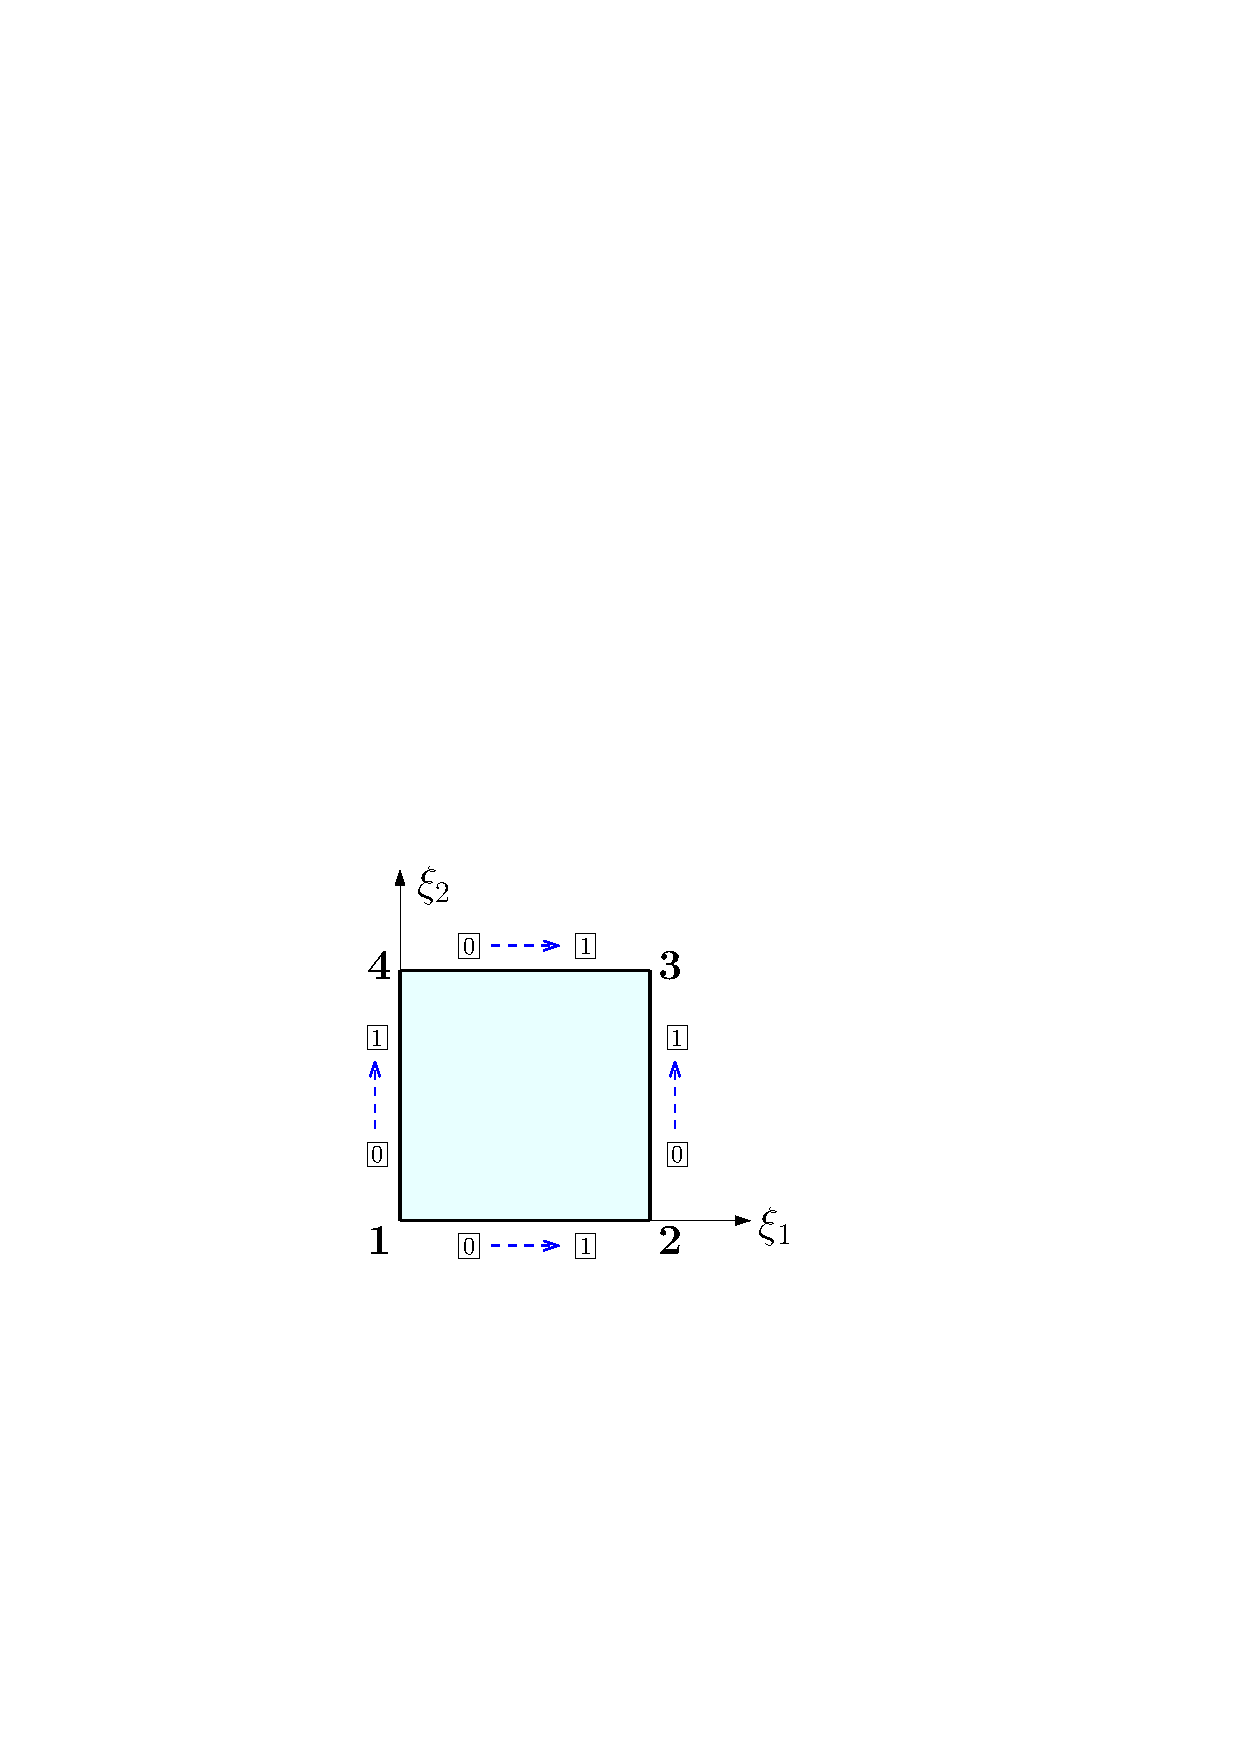
\includegraphics[scale=0.5]{./figures/MasterQuadOrientations.pdf}
\caption{Master quadrilateral with local edge orientations.}
\label{fig:MasterQuadOrientations}
\end{center}
\end{figure}

The master quadrilateral has a predefined \textit{local} orientation for each edge, which reperesents the $\oo=0$ case. 
These are illustrated in Figure \ref{fig:MasterQuadOrientations}.
They are \textit{our} choices for the local orientations.

%Recall each vertex has its own pair of 1D coordinates associated to it in the expression for the vertex functions (see \S\ref{sec:H1QuadVertices}). 
%That is, the vertex with coordinates $(a,b)$ is associated to the coordinates $\mu_a(\xi_1)$ and $\mu_b(\xi_2)$. %, while vertex 2 is associated to $\mu_1(\xi_1)$ and $\mu_0(\xi_2)$, and so on.
%When analizing a given edge, each of its two vertices have two 1D affine coordinates associated to them (so there is a total of four). Two of these will match and the other two will differ. 
%For example, for edge 12, with vertices 1 and 2, the coordinate $\mu_0(\xi_2)$ is shared by both vertices, but the coordinates $\mu_0(\xi_1)$ (related to vertex 1) and $\mu_1(\xi_1)$ (related to vertex 2) differ.
%The order in which these different coordinates are specified determines the $\oo=0$ local orientation.
%In edge 12, the local axis points from vertex 1 to vertex 2, so that the order of the coordinates should be $\mu_0(\xi_1)$ (related to vertex 1) followed by $\mu_1(\xi_1)$ (related to vertex 2).
Each edge has a local orientation described by the fixed ordering $\boxednum{0}\!\tdashto\boxednum{1}$.
This induces a master element \textit{local} edge vertex-ordering, which in turn determines a \textit{locally ordered} pair of affine coordinates, since, over a given edge, each master element vertex is linked to one affine coordinate.
For instance, over edge 12, $v_1$ is linked to $\mu_0(\xi_1)$ and $v_2$ linked to $\mu_1(\xi_1)$.
On this edge the induced master element \textit{local} ordering is $v_1\tdashto v_2$ (see Figure \ref{fig:MasterQuadOrientations}), meaning that the locally ordered pair is $\vec{\mu}_{01}(\xi_1)=(\mu_0(\xi_1),\mu_1(\xi_1))$.
The locally ordered pair represents the local coordinates, and it serves as the input of the edge local-to-global transformation $\sigma_\oo^\E$, which transforms them to a globally ordered pair (depending on the parameter $\oo$).
The globally ordered pair is then introduced into the edge ancillary functions of the edge shape functions, and the resulting functions are said to be \textit{orientation embedded} shape functions.
Thus, for example for edge 12 the orientation embedded $H^1$ edge functions are, 
\begin{equation*}
    \phi_i^\mathrm{e}(\xi)=\mu_0(\xi_2)\phi_i^\E\circ\sigma_\oo^\E(\vec{\mu}_{01}(\xi_1))
        =\begin{cases}
            \mu_0(\xi_2)\phi_i^\E\Big(\sigma_0^\E(\vec{\mu}_{01}(\xi_1))\Big)
            	=\mu_0(\xi_2)\phi_i^\E(\mu_0(\xi_1),\mu_1(\xi_1))\,\,\,\text{if }\oo=0\,,\\
            \mu_0(\xi_2)\phi_i^\E\Big(\sigma_1^\E(\vec{\mu}_{01}(\xi_1))\Big)
            	=\mu_0(\xi_2)\phi_i^{\e}(\mu_1(\xi_1),\mu_0(\xi_1))\,\,\,\text{if }\oo=1\,,
        \end{cases}
\end{equation*}
for $i=2,\ldots,p$.
This composition with $\sigma_\oo^\E$ naturally applies to all 2D edge functions in $H^1$ and $H(\mathrm{curl})$ and their differential forms. 
Hence, $\sigma_\oo^\E$ should be composed with $\phi_i^\E$, $\nabla\phi_i^\E$, $E_i^\E$ and $\nabla\times E_i^\E$ in \eqref{eq:QuadH1Edge} and \eqref{eq:QuadHcurlEdge}.


%Over each edge there is always a 1D affine coordinate duple $\vec{\mu}_{01}(\xi_a)=(\mu_0(\xi_a),\mu_1(\xi_a))$ for some $a=1,2$ which  induces a projection as described in \S\ref{sec:H1edgesQuad}.
%In fact, each affine coordinate is linked to a vertex of the edge being analyzed.
%For instance, in edge 12, $v_1$ is linked to $\mu_0(\xi_1)$, while $v_2$ is linked to $\mu_1(\xi_1)$.
%Now, the edge in question has a fixed local orientation described by a fixed local ordering $\boxednum{0}\!\tdashto\boxednum{1}$, which in turn induces a master element \textit{local} edge vertex-ordering.
%For edge 12, the master element \textit{local} edge vertex-ordering is $v_1\tdashto v_2$ (see Figure \ref{fig:MasterQuadOrientations}).
%This then generates an ordering of the affine coordinates, where first comes $\mu_0(\xi_1)$ linked to $v_1$ followed by $\mu_1(\xi_1)$ linked to $v_2$, so that the ordered affine coordinates are $\vec{\mu}_{01}(\xi_1)=(\mu_0(\xi_1),\mu_1(\xi_1))$ (as opposed to $\vec{\mu}_{10}(\xi_1)=(\mu_1(\xi_1),\mu_0(\xi_1))$ if $v_2\to v_1$).
%In this case, the affine coordinates are said to be \textit{locally ordered}, and in this form, they serve as the input for the edge orientation permutation function $\sigma_\oo^\E$.
%Indeed, the locally ordered affine coordinates represent the local $\oo=0$ orientation.
%%Note that the other alternative was that the master element ordering would have been 
%%Hence the \textit{ordered} pair of coordinates is $\vec{\mu}_{01}(\xi_1)=(\mu_0(\xi_1),\mu_1(\xi_1))$, as opposed to $\vec{\mu}_{10}(\xi_1)=(\mu_1(\xi_1),\mu_0(\xi_1))$.
%%The locally ordered
%The ancillary functions are then modified as described in \S\ref{sec:edgeorientations}, by composing first with $\sigma_\oo^\E$, which represents a local-to-global transformation.
%These modified functions are then replaced in the expressions of the shape functions to produce the \textit{orientation embedded} shape functions.
%Thus, for example for edge 12 the orientation embedded $H^1$ edge functions are, 
%\begin{equation*}
%    \phi_i^\mathrm{e}(\xi)=\mu_0(\xi_2)\phi_i^\E\circ\sigma_\oo^\E(\vec{\mu}_{01}(\xi_1))
%        =\begin{cases}
%            \mu_0(\xi_2)\phi_i^\E\Big(\sigma_0^\E(\vec{\mu}_{01}(\xi_1))\Big)
%            	=\mu_0(\xi_2)\phi_i^\E(\mu_0(\xi_1),\mu_1(\xi_1))\,\,\,\text{if }\oo=0\,,\\
%            \mu_0(\xi_2)\phi_i^\E\Big(\sigma_1^\E(\vec{\mu}_{01}(\xi_1))\Big)
%            	=\mu_0(\xi_2)\phi_i^{\e}(\mu_1(\xi_1),\mu_0(\xi_1))\,\,\,\text{if }\oo=1\,,
%        \end{cases}
%\end{equation*}
%for $i=2,\ldots,p$.
%Note that $\sigma_\oo^\E(\vec{\mu}_{01}(\xi_1))\neq\sigma_\oo^\E(\vec{\mu}_{10}(\xi_1))$, so, to be consistent with the local orientations, it is important that $\sigma_\oo^\E$ evaluates specifically the \textit{locally ordered} affine coordinates $\vec{\mu}_{01}(\xi_1)$.  
%These modifications naturally apply also to all 2D expressions involving $\nabla\phi_i^\E$, $E_i^\E$ and $\nabla\times E_i^\E$.
%%Clearly, the projection (as described in \S\ref{sec:H1edgesQuad}) and blending (given by $\mu_0(\xi_2)$) are unaffected by orientations.

\begin{figure}[!ht]
\begin{center}
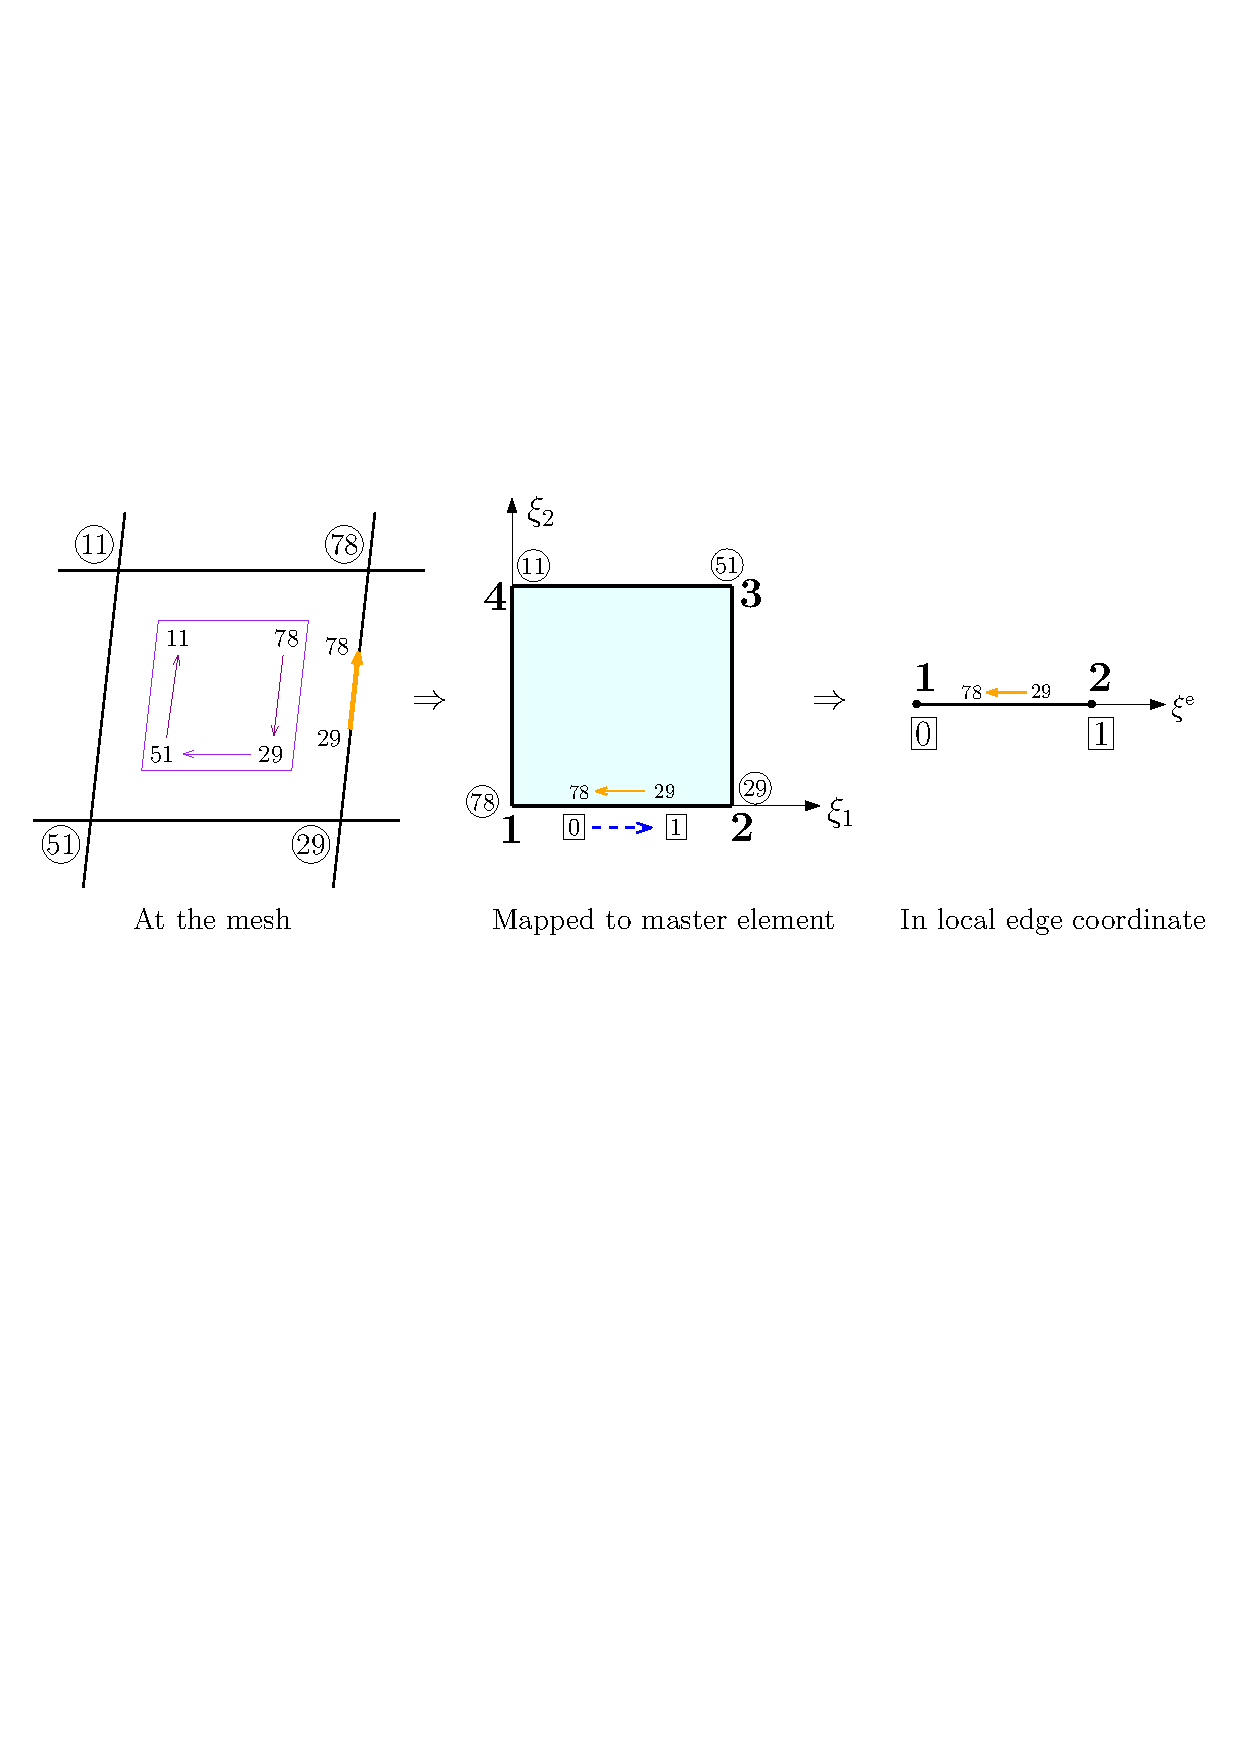
\includegraphics[scale=0.75]{./figures/QuadEdgeOrientExample.pdf}
\caption{A mesh with global edge orientations followed by transformations to master element and local edge coordinates.}
\label{fig:QuadEdgeOrientExample}
\end{center}
\end{figure}

Now, to see a more explicit example starting from the global mesh, consider Figure \ref{fig:QuadEdgeOrientExample}.
There, one can observe a quadrilateral in a mesh with vertices $11$, $29$, $51$ and $78$.
In 2D, Szabo's approach (implicitly) involves specifying a \textit{face vertex-ordering} at the mesh that determines the mapping to the master element, which has a fixed master element ordering $v_1\tto v_2\tto v_3\tto v_4$.
However, there is no independent edge vertex-ordering of each edge.
In this case, the face vertex-ordering at the mesh is shown to be $78\tto29\tto51\tto11$, and at the master element level it coincides with $v_1\tto v_2\tto v_3\tto v_4$.
%This is then mapped to the master element such that it coincides with the fixed master element ordering .
The novelty here is that additionally the mesh edge with vertices $78$ and $29$ also has a \textit{global} orientation given by the edge vertex-ordering $29\tto78$.
This edge is mapped to the master element edge 12 (as induced by the face vertex-ordering), and receives the induced master element \textit{global} ordering $v_2\tto v_1$. 
Clearly, the \textit{local} orientation, given by the induced \textit{local} ordering $v_1\tdashto v_2$, does not coincide with the \textit{global} orientation, meaning that the orientation parameter is $\oo=1$ for this master element edge.
Therefore, the orientation embedded $H^1$ edge shape functions would specifically be,
\begin{equation*}
    \phi_i^\mathrm{e}(\xi)=\mu_0(\xi_2)\phi_i^{\e}\circ\sigma_\oo^\E(\vec{\mu}_{01}(\xi_1))
            	=\mu_0(\xi_2)\phi_i^\E(\mu_1(\xi_1),\mu_0(\xi_1))\,,
\end{equation*}
for $i=2,\ldots,p$. 
The neighboring element in the mesh (also sharing vertices $29$ and $78$) might have a different face vertex-ordering, but it has the \textit{same} edge vertex-ordering at the mesh (the global orientation). 
This can result in another orientation parameter at the master element edge of the neighboring element, but by construction, the fact remains that when mapped back to the global mesh, the shape functions will be fully compatible along that shared edge.  
%For 2D quadrilaterals only edge orientations need to be considered to ensure compatibility.

%\paragraph{Edge Orientations.}
%To consider orientations, simply take a predefined $\oo=0$ orientation, which is determined only by looking at the master element axes and the predefined local edge axes for each edge, and replace $\phi_i^\E$ by $\phi_i^{\e,\oo}$. 
%For example, for edge 12, the local axis $\xi^\mathrm{e}$ is parallel to the master element axis $\xi_1$ and more importantly, it points in the \textit{same} direction. 
%This means the order of the entries in $\phi_i^{\e,\oo}$ is $(\mu_0(\xi_1),\mu_1(\xi_1))$ (and $\textit{not}$ $(\mu_1(\xi_1),\mu_0(\xi_1))$ which would apply if the master element axis and the local axis point in \textit{different} directions). 
%This defines the $\oo=0$ orientation.
%Hence, for edge 12, \eqref{eq:Quadphigeneral} becomes
%\begin{equation*}
%    \phi_i^\mathrm{e}(\xi)\!=\!\mu_0(\xi_2)\phi_i^{\e,\oo}(\mu_0(\xi_1),\mu_1(\xi_1))
%        \!=\!\!\begin{cases}
%            \mu_0(\xi_2)\phi_i^{\e,0}(\mu_0(\xi_1),\mu_1(\xi_1))\!
%            	=\!\mu_0(\xi_2)\phi_i^{\e}(\mu_0(\xi_1),\mu_1(\xi_1))\,\,\,\text{if }\oo=0\\
%            \mu_0(\xi_2)\phi_i^{\e,1}(\mu_0(\xi_1),\mu_1(\xi_1))\!
%            	=\!\mu_0(\xi_2)\phi_i^{\e}(\mu_1(\xi_1),\mu_0(\xi_1))\,\,\,\text{if }\oo=1\,,
%        \end{cases}
%\end{equation*}
%where \eqref{eq:edgeorientations} was used as the definition of $\phi_i^{\e,\oo}$. 
%The same applies to the gradients, and the other edge functions that follow in $H(\mathrm{curl})$ (which involve $E_i^\E$, to be defined later). 
%
%The predefined local edge axis is defined at the master element level.
%These predefined axes for each master element edge are shown in the Appendix.
%The predefined local axis explained above for edge 12 is actually the one utilized in our implementation.
%Naturally, in a different implementation one could decide to use other predefined local edge axes, and the $\oo=0$ orientation would change accordingly as explained above.
%In future examples we will only mention those predefined local edge axes that were used in our implementation (see Appendix).

\subsubsection{Quadrilateral Face Orientations Explained}
\label{sec:QuadFaceOrientations}

\begin{figure}[!ht]
\begin{center}
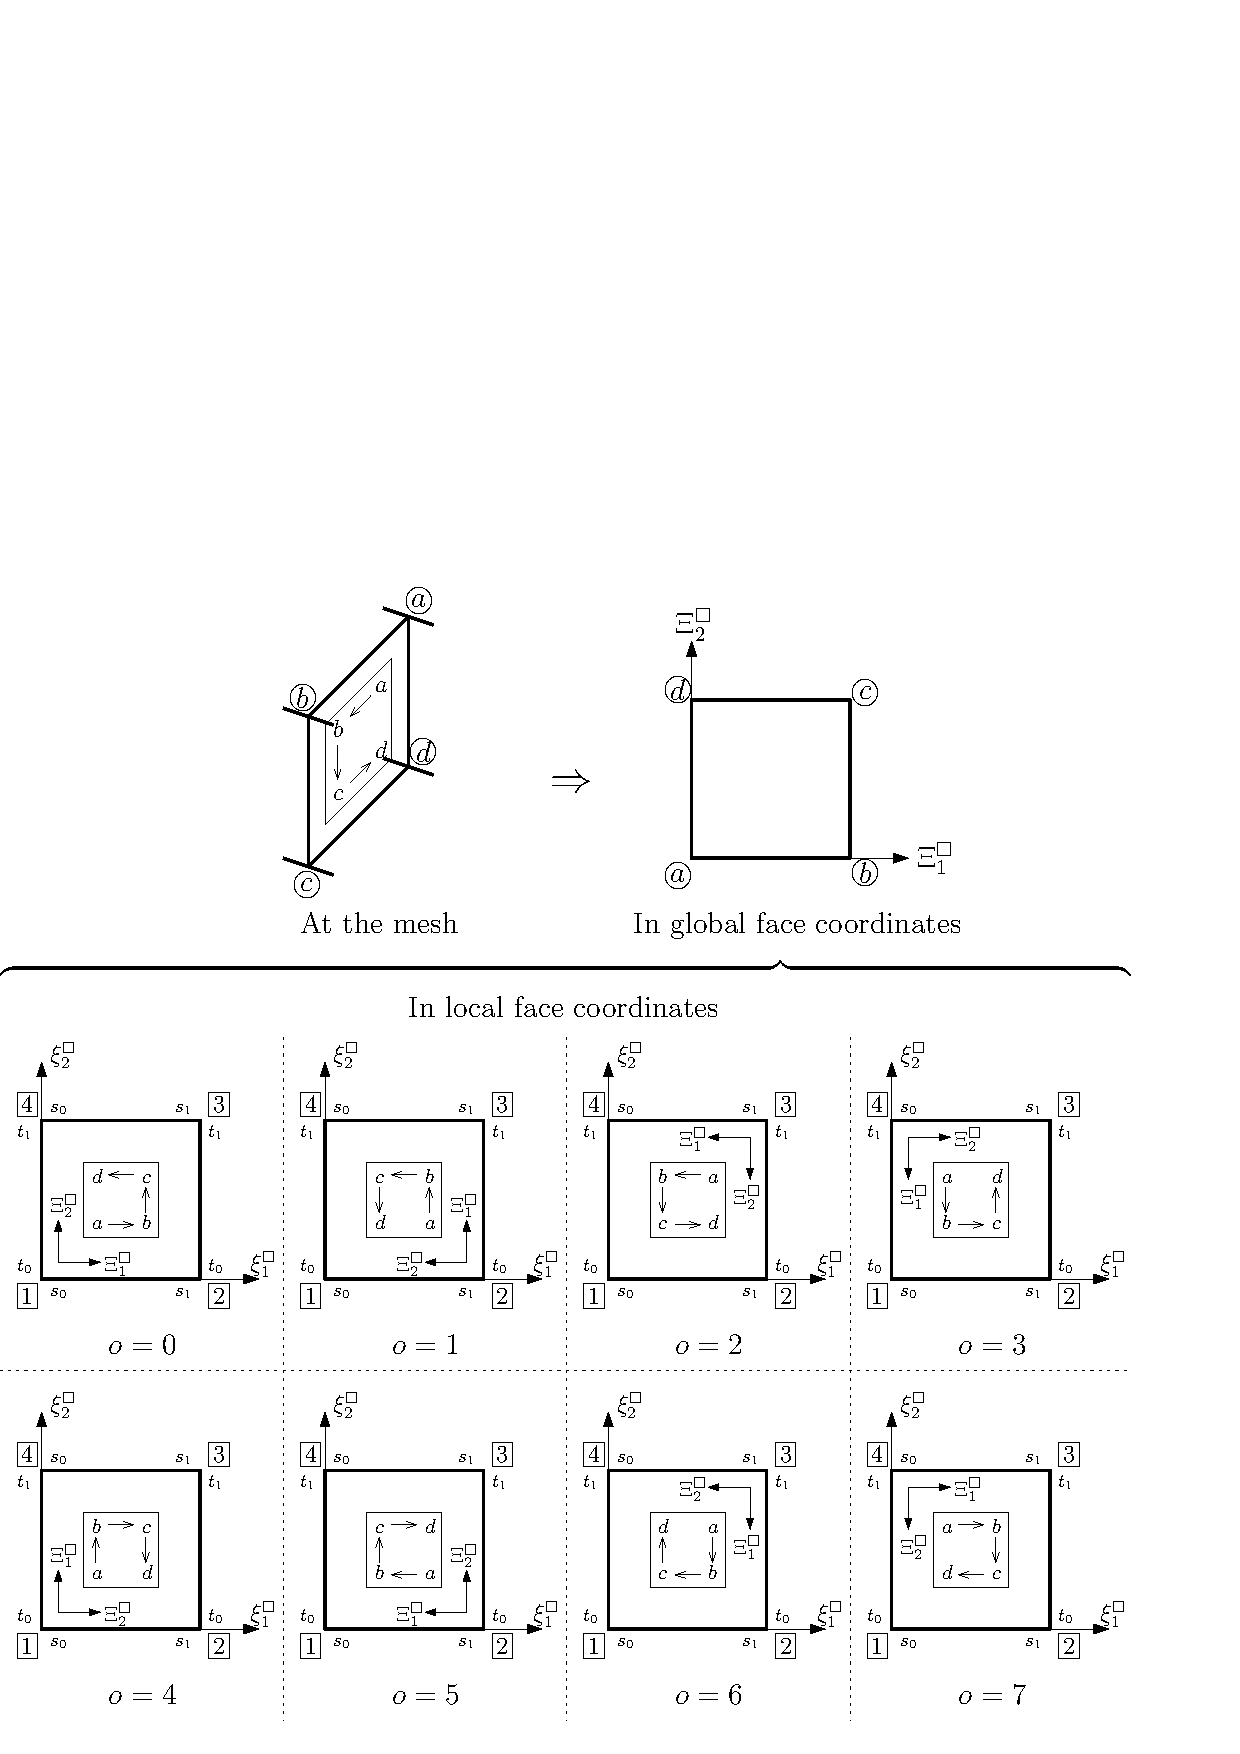
\includegraphics[scale=0.75]{./figures/OrientationsQuad.pdf}
\caption{Quadrilateral face orientations.}
\label{fig:orientationsquad}
\end{center}
\end{figure}

%For quadrilaterals it is not important to consider face orientations, since the boundary, which is shared with adjacent elements, is one dimensional.
%This means only edge orientations need to be considered.
%However, in three dimensions, the boundary is two dimensional.
%This means quadrilateral faces will be shared by adjacent elements.
%It is required to match the corresponding shape functions over these faces to satisfy the compatibility condition.
In 3D, as with edge orientations, each face at the mesh must be given its own \textit{global face orientation} to ensure full compatibility across the boundaries.
For quadrilaterals, this is represented by the global quadrilateral face coordinates $\Xi^\square=(\Xi_1^\square,\Xi_2^\square)$, or equivalently, by the \textit{global face vertex-ordering}.
For example, given a quadrilateral face in the mesh, a vertex-ordering of the form $a\tto b\tto c\tto d$ means the origin of $\Xi^\square$ is located at $a$, $\Xi_1^\square$ points from $a$ to $b$, and $\Xi_2^\square$ points from $a$ to $d$.
Meanwhile, at the master element, the mapped face has its own fixed \textit{local orientation}.
It is represented by the coordinates $\xi^\square=(\xi_1^\square,\xi_2^\square)$ or equivalently by the fixed \textit{local} ordering of the form $\boxednum{1}\!\tdashto\boxednum{2}\!\tdashto\boxednum{3}\!\tdashto\boxednum{4}$.
In general, the two systems of coordinates will not match, and this mismatch is represented by the orientation parameter $\oo$.
In fact, there are \textit{eight} possible orientations for quadrilateral faces, meaning $\oo=0,\ldots,7$.
These are all illustrated in Figure \ref{fig:orientationsquad}.


%Again, as with edge orientations, this will be done by embedding global face coordinate axes to each face in the mesh.
%These are denoted by $\Xi^\mathrm{f}=(\Xi_1^\mathrm{f},\Xi_2^\mathrm{f})$.
%Meanwhile at the master element level, each face (and edge) has a predefined local face (and edge) axis.
%For the faces, these local coordinates are denoted by $\xi^\mathrm{f}=(\xi_1^\mathrm{f},\xi_2^\mathrm{f})$.
%At the master element and given a face, it is clear that the predefined local face axis and the global face axis might not be the same.
%In fact, the main difficulty for the quadrilateral is that there are \textit{eight} possible orientations for each face.
%These are illustrated in Fig.~(\textit{add Figure}).
%They are referred to by the parameter $\oo$ which for quadrilateral faces goes from $0$ to $7$.

As with edges, the idea is to have a local-to-global transformation which depends on the orientation parameter $\oo$.
Here, the \textit{local} orientation is represented by the \textit{locally ordered} quadruple $(s_0,s_1,t_0,t_1)$ composed of the two pairs $(s_0,s_1)$ and $(t_0,t_1)$.
The \textit{first} pair, $(s_0,s_1)$, is a locally ordered pair corresponding to the \textit{first} local face coordinate $\xi_1^\square$ (which as an \textit{edge} coordinate has the local ordering $\boxednum{1}\!\tdashto\boxednum{2}$ or $\boxednum{4}\!\tdashto\boxednum{3}$).
The \textit{second} pair, $(t_0,t_1)$, is a locally ordered pair corresponding to the \textit{second} local face coordinate $\xi_2^\square$ (which as an \textit{edge} coordinate has the local ordering $\boxednum{1}\!\tdashto\boxednum{4}$ or $\boxednum{2}\!\tdashto\boxednum{3}$).
Meanwhile, the \textit{global} orientation is analogously represented by a \textit{globally ordered} quadruple composed of two pairs.
The first pair is a globally ordered pair corresponding to the first global face coordinate $\Xi_1^\square$, and similarly with the second pair.
For example, looking at Figure \ref{fig:orientationsquad}, when $\oo=1$, $\Xi_1^\square$ is associated to $(t_0,t_1)$, while $\Xi_2^\square$ is associated to $(s_1,s_0)$, so that the globally ordered quadruple is $(t_0,t_1,s_1,s_0)$.
This way, the local-to-global transformation is actually a permutation dependent on $\oo$ that can easily be determined by looking at Figure \ref{fig:orientationsquad}.
%As an example consider $\oo=1$, where $\Xi_1^\square$ is associated to the globally ordered pair $(t_0,t_1)$ (via $\boxednum{2}\!\tto\boxednum{3}$ or $\boxednum{1}\!\tto\boxednum{4}$), while $\Xi_2^\square$ is associated to $(s_1,s_0)$ (via $\boxednum{3}\!\tto\boxednum{4}$ or $\boxednum{2}\!\tto\boxednum{1}$).
%Therefore, the globally ordered quadruple is $(t_0,t_1,s_1,s_0)$.
%The full local-to-global transformation is described by the following permutation function. 

\begin{definition*}
Let $s_0$, $s_1$, $t_0$ and $t_1$ be arbitrary variables, and let $\oo=0,1,2,3,4,5,6,7$ be the quadrilateral face orientation parameter. 
The quadrilateral face orientation permutation function, $\sigma_\oo^\square$, is defined as
\begin{equation}
	\sigma_\oo^\square(s_0,s_1,t_0,t_1)=\begin{cases}
		\sigma_0^\square(s_0,s_1,t_0,t_1)=(s_0,s_1,t_0,t_1)&\quad\text{if  }\,\oo=0\,,\\
		\sigma_1^\square(s_0,s_1,t_0,t_1)=(t_0,t_1,s_1,s_0)&\quad\text{if  }\,\oo=1\,,\\
		\sigma_2^\square(s_0,s_1,t_0,t_1)=(s_1,s_0,t_1,t_0)&\quad\text{if  }\,\oo=2\,,\\
		\sigma_3^\square(s_0,s_1,t_0,t_1)=(t_1,t_0,s_0,s_1)&\quad\text{if  }\,\oo=3\,,\\
		\sigma_4^\square(s_0,s_1,t_0,t_1)=(t_0,t_1,s_0,s_1)&\quad\text{if  }\,\oo=4\,,\\
		\sigma_5^\square(s_0,s_1,t_0,t_1)=(s_1,s_0,t_0,t_1)&\quad\text{if  }\,\oo=5\,,\\
		\sigma_6^\square(s_0,s_1,t_0,t_1)=(t_1,t_0,s_1,s_0)&\quad\text{if  }\,\oo=6\,,\\
		\sigma_7^\square(s_0,s_1,t_0,t_1)=(s_0,s_1,t_1,t_0)&\quad\text{if  }\,\oo=7\,.\end{cases}\label{eq:orientQuadFace}
\end{equation}
\end{definition*}

%Clearly, ``outer'' permutations (of the pairs) occur when the global edge axis $\Xi_1^\square$ is parallel to $\xi_2^\square$ (or equivalently if $\Xi_2^\square$ is parallel to $\xi_1^\square$).
%In this case, the axes are said to be \textit{swapped}.
%On the other hand, inner permutations represent the alignment of the parallel axes.
%If inner permutations are applied \textit{after} outer permutations, then the inner permutation of the first pair represents whether the \textit{global} $\Xi_1^\square$ axis points in the same direction as the parallel local axis (and similarly with the second pair).
%If inner permutations are applied \textit{before} outer permutations, then the inner permutation of the first pair represents whether the \textit{local} $\xi_1^\square$ axis points in the same direction as the parallel global axis (and similarly with the second pair).

As with edges, all that is required is to compose the \textit{quadrilateral face} ancillary functions and their differential form (those with superscript $\square$) with the local-to-global transformation given by $\sigma_\oo^\square$.
This should be done in all 3D shape functions associated to quadrilateral faces.
More concrete examples will be given in the 3D elements as the document progresses.
%Thus, in 3D, all instances of $\phi_i^\E$ and $\nabla\phi_i^\E$ in the shape functions should be replaced with $\phi_i^\E\circ\sigma_\oo^\E$ and $\nabla\phi_i^\E\circ\sigma_\oo^\E$ respectively.
%The resulting functions are then said to be \textit{orientation embedded} shape functions.
%More concrete examples will be given in the 2D and 3D elements as the document progresses.

%Fortunately, these orientations will be handled by a simple matter of permuting the entries of the quadrilateral face functions: $\phi_{ij}^\square$, $E_{ij}^{\square_I}$, $E_{ij}^{\square_{II}}$, and in the future $V_{ij}^\square$.
%However, it should be mentioned that nontrivial pullback transforms are ocurring internally (but automatically) in the functions when the entries are permuted.
%%This is particularly true for $E_{ij}^{\square_I}$, $E_{ij}^{\square_{II}}$ and $V_{ij}^\square$.
%To better explain the nature of these permutations, define the auxiliary permutation function
%\begin{equation}
%    \begin{alignedat}{2}
%        \vec{\kappa}:\{0,1,2,3,4,5,6,7\}&\,\longrightarrow\,\{0,1\}\times\{0,1\}\times\{0,1\}\\
%        \oo\,&\,\longmapsto\,(\kappa_1(\oo),\kappa_2(\oo),\kappa_3(\oo))\,.
%    \end{alignedat}
%\end{equation}
%
%\begin{table}[!ht]
%\begin{center}
%\begin{tabular}
%{|c|c|c|c|}\hline
%$\oo$ & $\kappa_1(\oo)$ & $\kappa_2(\oo)$  &  $\kappa_3(\oo)$ \\\hline\hline
%0 &0 & 0  & 0 \\\hline
%1 &1 & 1  & 0 \\\hline
%2 &0 & 1  & 1 \\\hline
%3 &1 & 0  & 1 \\\hline
%4 &1 & 0  & 0 \\\hline
%5 &0 & 1  & 0 \\\hline
%6 &1 & 1  & 1 \\\hline
%7 &0 & 0  & 1 \\\hline\hline
%\end{tabular}
%\caption{Function $\vec{\kappa}$.
%\label{table:functionkappa}}
%\end{center}
%\end{table}
%
%
%The first component, $\kappa_1(\oo)$, will denote whether the global axes $\Xi_1^\mathrm{f},\Xi_2^\mathrm{f}$ are \textit{swapped} with respect to the fixed local axes $\xi_1^\mathrm{f},\xi_2^\mathrm{f}$.
%The second component, $\kappa_2(\oo)$ will denote whether the local $\xi_1^\mathrm{f}$ axis points in the same direction as the parallel global axis.
%Similarly, the third component, $\kappa_3(\oo)$ will represent whether the local $\xi_2^\mathrm{f}$ axis points in the same direction as the parallel global axis.
%For example, when $\oo=1$ the $\xi_1^\mathrm{f}$ axis is parallel to the $\Xi_2^\mathrm{f}$ axis, and similarly with $\xi_2^\mathrm{f}$ and $\Xi_1^\mathrm{f}$ axes, so in this case the axes are swapped (see Fig.~(\textit{put Figure})).
%Also, $\xi_1^\mathrm{f}$ and $\Xi_2^\mathrm{f}$ do not point in the same direction, but $\xi_2^\mathrm{f}$ and $\Xi_1^\mathrm{f}$ do.
%The values of the function are presented in Table \ref{table:functionkappa}.
%
%This provides a natural setting to replace the functions $\phi_{ij}^\square$, $E_{ij}^{\square_I}$, $E_{ij}^{\square_{II}}$ and $V_{ij}^\square$ with the new families of functions $\phi_{ij}^{\square,\oo}$, $E_{ij}^{\square_I,\oo}$, $E_{ij}^{\square_{II},\oo}$ and $V_{ij}^{\square,\oo}$ and their respective differentiated versions. Take for example $E_{ij}^{\square_I,\oo}$. Denoting $\neg\kappa_i(\oo)=\mathrm{mod}(\kappa_i(\oo)+1,2)$ as the opposite of $\kappa_i(\oo)$, allows to compactly write the new family of functions as
%\begin{equation}
%    E_{ij}^{\square_I,\oo}(s_0^{(0)},s_1^{(0)},s_0^{(1)},s_1^{(1)})=
%        E_{ij}^{\square_I,\oo}(s_{\kappa_2(\oo)}^{(\kappa_1(\oo))},s_{\neg\kappa_2(\oo)}^{(\kappa_1(\oo))},
%            s_{\kappa_3(\oo)}^{(\neg\kappa_1(\oo))},s_{\neg\kappa_3(\oo)}^{(\neg\kappa_1(\oo))})\,,
%\end{equation}
%for all $i=0,\ldots,p_{s^{(\kappa_1(\oo))}}-1$ and $j=2,\ldots,p_{s^{(\neg\kappa_1(\oo))}}$. More spread out, and perhaps clearer,
%\begin{equation}
%    E_{ij}^{\square_I,\oo}(s_0,s_1,t_0,t_1)=\begin{cases}
%    E_{ij}^{\square_I,0}(s_0,s_1,t_0,t_1)=E_{ij}^{\square_I}(s_0,s_1,t_0,t_1)&\quad\text{if  }\,\oo=0\\
%    E_{ij}^{\square_I,1}(s_0,s_1,t_0,t_1)=E_{ij}^{\square_I}(t_1,t_0,s_0,s_1)&\quad\text{if  }\,\oo=1\\
%    E_{ij}^{\square_I,2}(s_0,s_1,t_0,t_1)=E_{ij}^{\square_I}(s_1,s_0,t_1,t_0)&\quad\text{if  }\,\oo=2\\
%    E_{ij}^{\square_I,3}(s_0,s_1,t_0,t_1)=E_{ij}^{\square_I}(t_0,t_1,s_1,s_0)&\quad\text{if  }\,\oo=3\\
%    E_{ij}^{\square_I,4}(s_0,s_1,t_0,t_1)=E_{ij}^{\square_I}(t_0,t_1,s_0,s_1)&\quad\text{if  }\,\oo=4\\
%    E_{ij}^{\square_I,5}(s_0,s_1,t_0,t_1)=E_{ij}^{\square_I}(s_1,s_0,t_0,t_1)&\quad\text{if  }\,\oo=5\\
%    E_{ij}^{\square_I,6}(s_0,s_1,t_0,t_1)=E_{ij}^{\square_I}(t_1,t_0,s_1,s_0)&\quad\text{if  }\,\oo=6\\
%    E_{ij}^{\square_I,7}(s_0,s_1,t_0,t_1)=E_{ij}^{\square_I}(s_0,s_1,t_1,t_0)&\quad\text{if  }\,\oo=7\,,
%    \end{cases}
%\end{equation}
%where the numbering is
%\begin{equation}
%    \begin{alignedat}{2}
%            i&=0,\ldots,p_s-1\,,\qquad j=2,\ldots,p_t\,,\qquad\,\text{if }\,\kappa_1(\oo)=0\,,\\
%            i&=0,\ldots,p_t-1\,,\qquad j=2,\ldots,p_s\,,\qquad\,\text{if }\,\kappa_1(\oo)=1\,.
%    \end{alignedat}
%\end{equation}

%Section 5
\newpage
%\addtocontents{toc}{\protect\newpage}%No page break at TOC
\section{Triangle}
\label{sec:Tri}

\begin{figure}[!ht]
\begin{center}
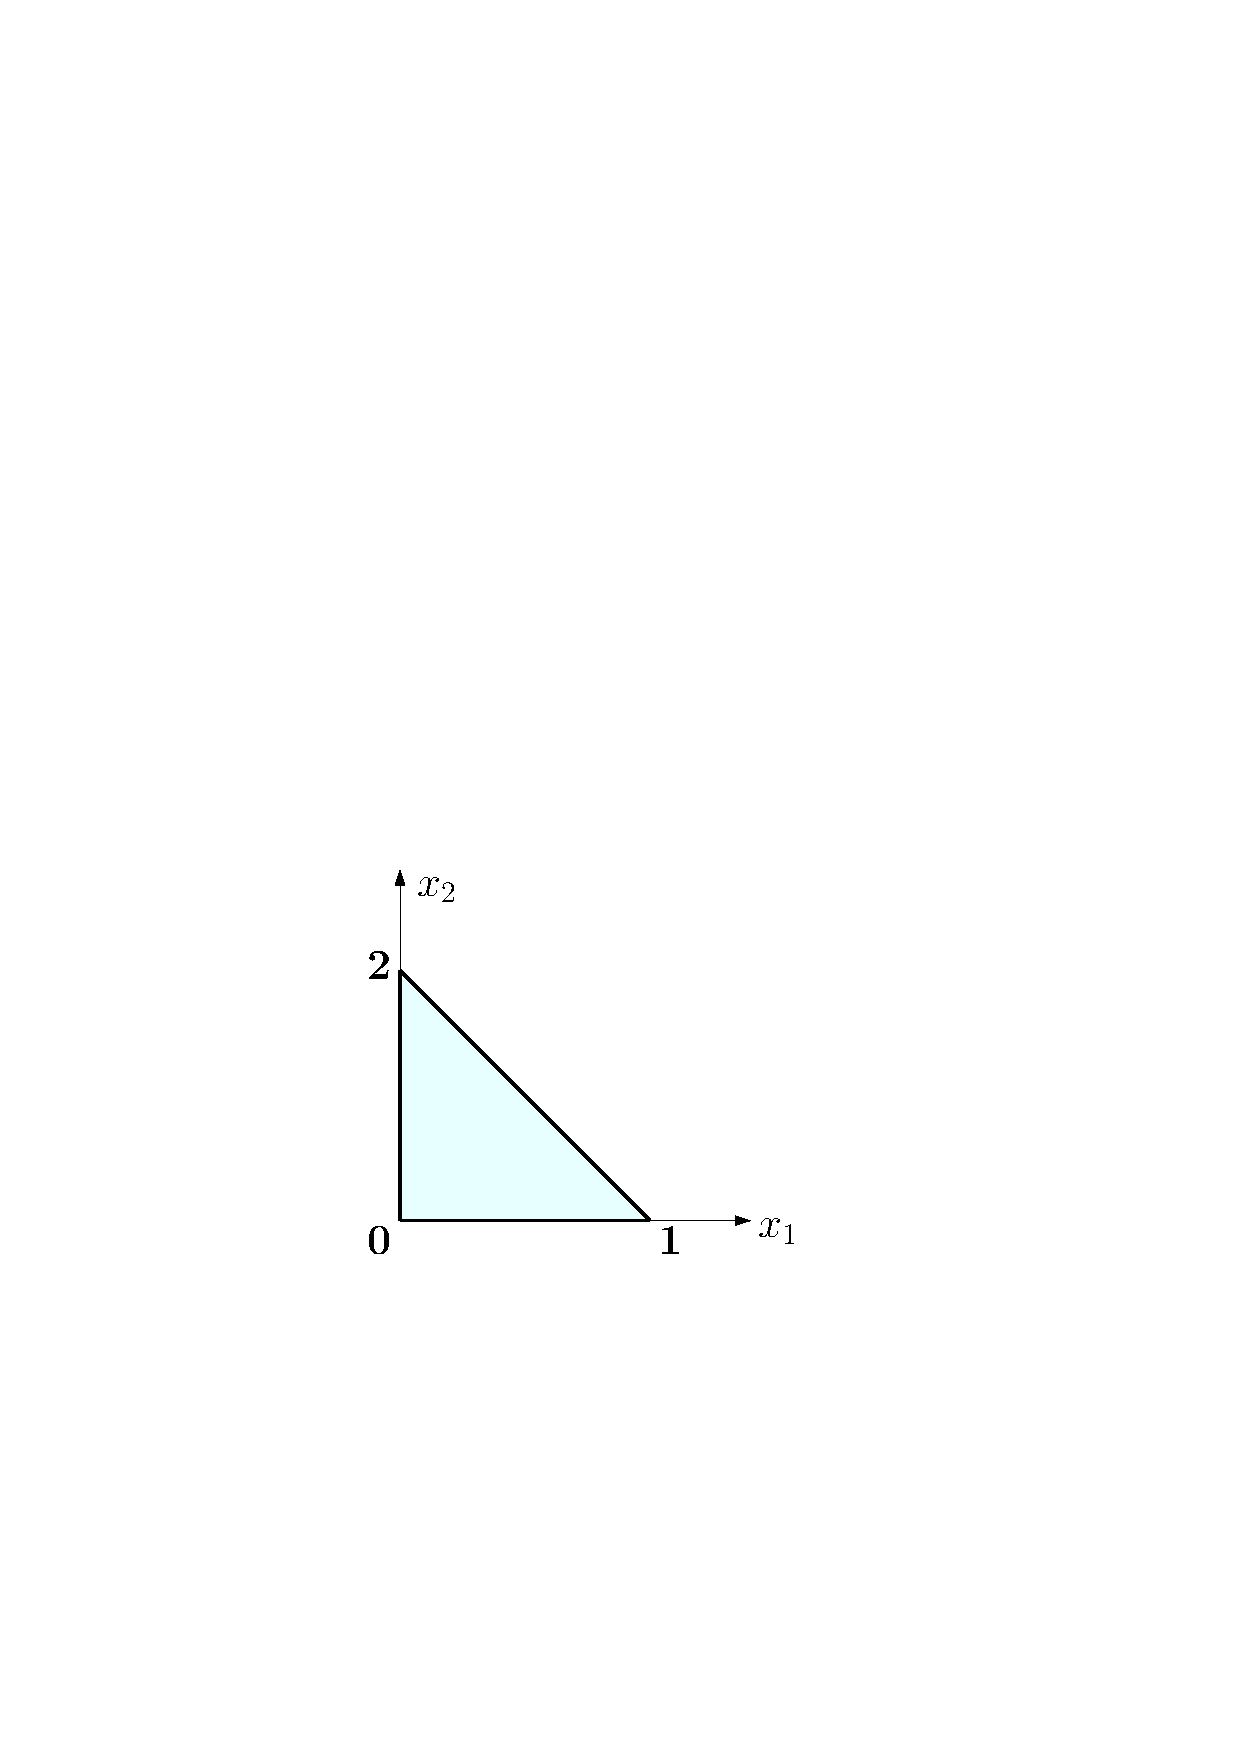
\includegraphics[scale=0.5]{./figures/MasterTri.pdf}
\caption{Master triangle with numbered vertices.}
\label{fig:MasterTriangle}
\end{center}
\end{figure}

The triangle is the 2D simplex.
The master element for triangles in the $x=(x_1,x_2)$ space is the set $\{x\in\R^2:x_1>0,x_2>0,x_1+x_2<1\}$. 
It is illustrated in Figure \ref{fig:MasterTriangle}.

Denote vertex $a$ by $v_a$, so that $v_0=(0,0)$, $v_1=(1,0)$ and $v_2=(0,1)$.
As described in \S\ref{sec:affinecoordinates}, the 2D affine coordinates, $\nu_0$, $\nu_1$ and $\nu_2$, can be easily calculated for this master triangle:
\begin{equation}
	%\begin{aligned}
	\nu_0(x)=1-x_1-x_2\,,\qquad
	\nu_1(x)=x_1\,,\qquad
	\nu_2(x)=x_2\,.
	%\begin{aligned}
\end{equation}
Their gradients are
\begin{equation}
\nabla\nu_0(x)=\Big(\begin{smallmatrix}-1\\[2pt]-1\end{smallmatrix}\Big)\,,\qquad
\nabla\nu_1(x)=\Big(\begin{smallmatrix}1\\[2pt]0\end{smallmatrix}\Big)\,,\qquad
\nabla\nu_2(x)=\Big(\begin{smallmatrix}0\\[2pt]1\end{smallmatrix}\Big)\,.
\end{equation}

Like the quadrilateral and segment, the triangle exhibits a correspondence of its vertices and its affine coordinates.
Looking at the formula $x=\nu_0(x)v_0+\nu_1(x)v_1+\nu_2(x)v_2$ this relation is evident, in the sense that each vertex is linked to \textit{one} affine coordinate (its corresponding weight).
For example $v_1$ is linked to the affine coordinate $\nu_1(x)$, and indeed it takes the value $1$ when $x=v_1$ while it is zero at the other two vertices.
%In two dimensions, we denote by $\hat\Delta$ as the master triangle. The master element is indicated in figure[]. We shall use the following notation for affine coordinates: $s_n=\nu_n$, $n\in\{0,1,2\}$ will denote affine coordinates for a triangle. Also, by ``edge 0-1'' we mean the edge defined by $\nu_0,\nu_1$. Other edges are similarly defined. Observe that
%\be
%\sum_{n=0}^2 \nu_n( x)=1\,,
%\ee
%and
%\be
%\nu_n( x)\ge0\,,
%\ee
%for all $ x\in\hat\Delta$.

\subsubsection*{Exact Sequence}


%Also, $(\mathcal{P}^p)^2=\mathcal{P}^p\times\mathcal{P}^p$ and similarly with $(\tilde{\mathcal{P}}^p)^2$.

%i.e., vector space of 2-tuples of elements in $\mathcal{P}^p$. Furthermore, define $\tilde{\mathcal{P}}^{p} = \tilde{\mathcal{P}}^{p} (\hat\Delta)$ to be the subspace of homogeneous polynomials of order $p$ on $\hat\Delta$. The space $\left(\tilde{\mathcal{P}}^{p}\right)^2$ is defined similarly.

%It is our intent to reproduce the\footnote{%Given the 2D rotation $R:(x_1,x_2)\mapsto(x_2,-x_1)$, observe that $R:H(\text{curl}) \to H(\text{div})$ is an isomorphism. Moreover, $\nabla\times = R\nabla$, $\text{curl}(\,\cdot\,) = \nabla\cdot R(\,\cdot\,)$.
%NEW FOOTNOTE. REFERENCE INTRODUCTION.} 2D exact sequence(s)

As with the quadrilateral, the triangle will have 2D discrete polynomial exact sequences that represent the continuous exact sequence \eqref{eq:2DExactSeq} and its rotated analogue \eqref{eq:2DExactSeqRotated}. 
They are
%\begin{equation}
%\begin{alignedat}{4}
%    &W^{p} \xrightarrow{\,\,\nabla\,\,} &Q^{p} \xrightarrow{\nabla\times} &&Y^{p} \,,\\
%    &W^{p} \xrightarrow{\mathrm{curl}\,} &V^{p} \xrightarrow{\,\nabla\cdot\,} &&Y^{p} \,,
%\end{alignedat}
%\end{equation}
%where more specifically the spaces \citeyearpar{Nedelec80} of the first type for the quadrilateral are utilized:
%\begin{equation}
%    \begin{aligned}
%    W^{p,q} & = \mathcal{Q}^{p,q}= \mathcal{P}^p(\xi_1)\otimes \mathcal{P}^q(\xi_2)\,, \\
%    Q^{p,q} & = \mathcal{Q}^{p-1,q} \times\mathcal{Q}^{p,q-1}\,, \\
%    V^{p,q} & = \mathcal{Q}^{p,q-1} \times\mathcal{Q}^{p-1,q}\,, \\
%    Y^{p,q} & = \mathcal{Q}^{p-1,q-1}\,.
%    \end{aligned}
%\end{equation}
%
%Let $\mathcal{P}^p =\mathcal{P}^p(x_1,x_2)$ be the space of polynomials of total order $p$ in the $x=(x_1,x_2)$ space. 
%Recall the 2D exact sequence for simply connected domains \eqref{eq:2DExactSeq} and its rotated analogue \eqref{eq:2DExactSeqRotated}:
%\begin{equation}
%\begin{alignedat}{4}
%	&H^1 \xrightarrow{\,\,\nabla\,\,} &&H(\mathrm{curl}) \xrightarrow{\nabla\times} \,&L^2 \,,\\
%	&H^1 \xrightarrow{\mathrm{curl}\,}\, &&H(\mathrm{div})\, \xrightarrow{\,\,\nabla\cdot\,\,} &L^2 \,.
%\end{alignedat}
%\end{equation}
%
%The corresponding polynomial exact sequences are
\begin{equation}
\begin{alignedat}{4}
    &\mathcal{P}^p \xrightarrow{\,\,\nabla\,\,} &\mathcal{N}^p \xrightarrow{\nabla\times} && \mathcal{P}^{p-1} \,,\\
    &\mathcal{P}^p \xrightarrow{\mathrm{curl}\,} &\mathcal{RT}^p \xrightarrow{\,\nabla\cdot\,} &&\mathcal{P}^{p-1} \,,
    \label{eq:EStriangle}
\end{alignedat}
\end{equation}
where $\mathcal{P}^p =\mathcal{P}^p(x_1,x_2)$ is the space of polynomials of total order $p$.
The spaces $\mathcal{N}^p$ and $\mathcal{RT}^p$ are the N\'{e}d\'{e}lec and Raviart-Thomas spaces for simplices:
\begin{align}
	\label{eq:NedelecSpace}
	\mathcal{N}^p&=(\mathcal{P}^{p-1})^N\oplus\Big\{E\in(\tilde{\mathcal{P}}^{p})^N: x\cdot E(x)=0\,\text{ for all } x\in\R^N\Big\}\,,\\
	\label{eq:RaviartThomasSpace}
	\mathcal{RT}^p&=(\mathcal{P}^{p-1})^N\oplus\Big\{V\in(\tilde{\mathcal{P}}^{p})^N: V(x)=\phi(x)x
		\, \text{ with }\phi\in\tilde{\mathcal{P}}^{p-1}\,\text{ and }x\in\R^N\Big\} \,.
\end{align}
In the case of the triangle, the number of spatial dimensions is $N=2$.
%, and in fact $\mathcal{N}^p$ and $\mathcal{RT}^p$ are ``rotations'' of each other.
%That is, $\mathcal{RT}^p=\{V=\Big(\begin{smallmatrix}0&1\\[2pt]-1&0\end{smallmatrix}\Big)E=: E\in\mathcal{N}^p\}$
Note the sequence has an overall drop in polynomial order of one. 
This makes it compatible with the construction presented for the quadrilateral.
Moreover, all of the spaces in the exact sequences above are invariant under affine transformations. 
This implies the exact sequence takes the same form for any given triangle (provided it is mapped via an affine transformation from the master triangle, which is always possible).
%That is, the pullback of an affine transformation brings $\mathcal{N}^p(\hat\Delta)$ onto $\mathcal{N}^p(\Delta)$, etc. Here, $\Delta$ denotes the triangle in physical space (i.e., the physical element).

\subsection{\texorpdfstring{$H^1$}{H1} Shape Functions}
%In two dimensions, the trace of $H^1$ functions is the value of the function itself along the boundary.
%Hence, all vertex functions vanish at all nonadjacent edges, and all edge functions should vanish at all other edges.
%The bubbles will vanish at all edges.

All shape functions defined here will lie in $\mathcal{P}^{p}$, which has dimension $\frac{1}{2}(p+2)(p+1)$. 
Moreover, a careful count of the linearly independent shape functions will coincide with that dimension, so that indeed the space is spanned.

\subsubsection{\texorpdfstring{$H^1$}{H1} Vertices}
%Affine coordinates in two dimensions will be denoted by $\nu_0$, $\nu_1$ and $\nu_2$. They are written explicitly for our master triangle:
%\begin{equation}
%	%\begin{aligned}
%	\nu_0(x)=1-x_1-x_2\,,\qquad
%	\nu_1(x)=x_1\,,\qquad
%	\nu_2(x)=x_2\,.
%	%\begin{aligned}
%\end{equation}
%Their gradients are
%\begin{equation}
%\nabla\nu_0(x)=\Big(\begin{smallmatrix}-1\\[2pt]-1\end{smallmatrix}\Big)\,,\qquad
%\nabla\nu_1(x)=\Big(\begin{smallmatrix}1\\[2pt]0\end{smallmatrix}\Big)\,,\qquad
%\nabla\nu_2(x)=\Big(\begin{smallmatrix}0\\[2pt]1\end{smallmatrix}\Big)\,.
%\end{equation}
%Take note of the above, since they will be used explicitly or implicitly in the computations of shape functions throughout this section.

In this case, for a given vertex, the associated shape function will be its related affine coordinate.
For example, $v_0$ is linked to $\nu_0(x)$, so its associated vertex function is simply 
\begin{equation*}
	\phi^\mathrm{v}(x)=\nu_0(x)\,.
\end{equation*}
As expected, it vanishes at the disjoint opposite edge 12 and its trace over the adjacent edges is a 1D $H^1$ vertex function associated to the vertex. 
Indeed, the traces are explicitly,
\begin{equation*}
	\nu_0(x)|_{x_2=0}=1-x_1=\mu_0(x_1)\,,\qquad\nu_0(x)|_{1-x_1-x_2=0}=0\,,\qquad\nu_0(x)|_{x_1=0}=1-x_2=\mu_0(x_2)\,. 
\end{equation*}
Lastly, the function decays linearly and is in the lowest order possible space, $\mathcal{P}^1$, so that it respects the hierarchy in $p$.

In general, the vertex functions and their gradient are,
\begin{equation}
    \phi^\mathrm{v}(x)=\nu_a(x)\,,\qquad\quad\nabla\phi^\mathrm{v}(x)=\nabla\nu_a(x)\,,
\end{equation}
for $a=0,1,2$.
There are a total of $3$ vertex functions (one for each vertex).
%
%
%The $H^1$ vertex shape functions will precisely be these affine coordinates. 
%They are presented next with their gradients
%\begin{equation}
%	\phi^\mathrm{v}(x)=\nu_a(x)\,,\qquad\nabla\phi^\mathrm{v}(x)=\nabla\nu_a(x)\,,\qquad a=0,1,2\,.
%\label{eq:H1_CountingSimplexVert}
%\end{equation}
%Clearly the vertex shape functions vanish at all vertices except vertex $a$ for $a=0,1,2$. By linearity, their trace is of the right form. That is, it satisfies the vanishing properties and is compatible with the vertex functions of the segment (and thus with edges of the quadrilateral). Take for example vertex 0 which has vertex function $\nu_0(x)$. The traces are
%\begin{equation*}
%	\nu_0(x)|_{x_2=0}=1-x_1=\mu_0(x_1)\,,\qquad\nu_0(x)|_{x_2=1-x_1}=0\,,\qquad\nu_0(x)|_{x_1=0}=1-x_2=\mu_0(x_2)\,, 
%\end{equation*}
%so that the function vanishes at the only (opposite) nonadjacent edge, and it has the form $\mu_b(x_a)$ for some $a=1,2$ and $b=0,1$ for the other two edges (which are compatible with the segment vertex functions).

\subsubsection{\texorpdfstring{$H^1$}{H1} Edges}
\label{sec:H1edgesTri}

For the construction of the edge functions consider edge 01 as an example.
To satisfy compatibility with the quadrilateral, the shape functions should have $\phi_i^\E(\vec{\mu}_{01}(x_1))$ as the trace over edge 01, and be zero at the two other edges.
Additionally, they should be polynomial (they should be in $\mathcal{P}^p$).

Unfortunately, at first sight the construction is not trivial since many intuitive approaches lead to violating some of the required properties mentioned above.
This is in large part due to the fact that the triangle is \textit{not} a Cartesian product of lower dimensional elements.
Luckily, these issues are all solved by the process of homogenization, which is viewed as a particular extension of the lower dimensional edge functions $\phi_i^\E(\vec{\mu}_{01}(x_1))$.
The idea is to exploit the 2D \textit{triangle} affine coordinates associated to edge 01, which are $\nu_0$ and $\nu_1$ (those linked to the vertices $v_0$ and $v_1$ which compose the edge).
Indeed, let the shape functions for this edge be
\begin{equation*}
    \phi_i^\mathrm{e}(x)=\phi_i^\E(\vec{\nu}_{01}(x))=[L_i](\vec{\nu}_{01}(x))
    	=(\nu_0(x)+\nu_1(x))^i
    		[L_i]\Big(\textstyle{\frac{\nu_0(x)}{\nu_0(x)+\nu_1(x)}},\textstyle{\frac{\nu_1(x)}{\nu_0(x)+\nu_1(x)}}\Big)\,,
\end{equation*}
with $i=2,\ldots,p$.
Here, property \eqref{eq:ScalingProperty} was used.
Notice that $\nu_2=0$ is the equation for edge 01 and similarly with the other edges.
Hence, using the vanishing properties of $\phi_i^\E$ in \eqref{eq:phiEvanishing}, it follows that the trace properties are satisfied:
\begin{alignat*}{3}
    &\phi_i^\mathrm{e}(x)|_{x_2=0}&&=\phi_i^\E(\vec{\nu}_{01}(x))|_{\nu_2=0}=\phi_i^\E(\vec{\mu}_{01}(x_1))\,,\\
    &\phi_i^\mathrm{e}(x)|_{1-x_1-x_2=0}&&=\phi_i^\E(\vec{\nu}_{01}(x))|_{\nu_0=0}=\phi_i^\E(0,\mu_1(x_1))=0\,,\\
  	&\phi_i^\mathrm{e}(x)|_{x_1=0}&&=\phi_i^\E(\vec{\nu}_{01}(x))|_{\nu_1=0}=\phi_i^\E(\mu_0(x_2),0)=0\,.
\end{alignat*}
In this case, the decay of each shape function is represented by the nonlinear function $(\nu_0(x)+\nu_1(x))^i$, which comes hidden within the homogenization.
Additionally, $\phi_i^\E(\vec{\nu}_{01})\in\tilde{\mathcal{P}}^i(\nu_0,\nu_1)$ by homogenization while $\nu_0(x),\nu_1(x)\in\mathcal{P}^1(x)$, meaning that the edge functions $\phi_i^\E(\vec{\nu}_{01}(x))$ are in $\mathcal{P}^i(x)\subseteq\mathcal{P}^p(x)$ as required.
%To construct these edge functions one must be aware that the trace over the other two edges should vanish, while the trace over the edge itself should have the correct form compatible with the segment edge bubbles. 
%That is, the trace should be of the form $L_i$ for the given edge. 
%
%This amounts to starting with $L_i$ over the given edge and then choosing a correct blending function which extends (or lifts) it to the rest of the element, while respecting the vanishing conditions. 
%This extension should also be polynomial (it should be in $\mathcal{P}^p$). 
%Fortunately, all these criteria are met by the process of \textit{homogenization} (see \textit{cite homog}).
%
%To see this, take for example edge 01, and the related affine coordinates $\nu_0$ and $\nu_1$. Notice their restriction to edge 01 is of the form 
%\begin{equation*}
%	\nu_0(x)|_{x_2=0}=\mu_0(x_1)\,,\qquad\quad \nu_1(x)|_{x_2=0}=\mu_1(x_1)\,.
%\end{equation*}
%This might suggest a similar approach to the quadrilateral at first, where one seeks to work with 1D affine coordinates and a linear blending function. 
%However, attempts show that there is no easy fix. 
%This is due to the fact that the triangle is \textit{not} a tensor product of two line segments. 
%Indeed, ideally one should try to exploit the geometry by using the 2D affine coordinates directly.
%Following \textit{cite Sch\"{o}berl}, this can be achieved by a proper scaling of the original polynomial.
%In the context of this work, this process is called homogenization and results in
%\begin{equation*}
%	[L_i](\nu_0,\nu_1)=L_i(\nu_1;\nu_0+\nu_1)
%	=\underbrace{(\nu_0+\nu_1)^i}_{\text{blend}}
%		\underbrace{L_i(\underbrace{\textstyle{\frac{\nu_1}{\nu_0+\nu_1}}}_{\text{project}})}_{\text{evaluate}}\,.
%\end{equation*}
%By construction, $[L_i](\nu_0,\nu_1)$ is homogeneous in $\nu_0$ and $\nu_1$ of total order $i$, so that $[L_i](\nu_0(x),\nu_1(x))\in\mathcal{P}^i$. 

\begin{figure}[!ht]
\begin{center}
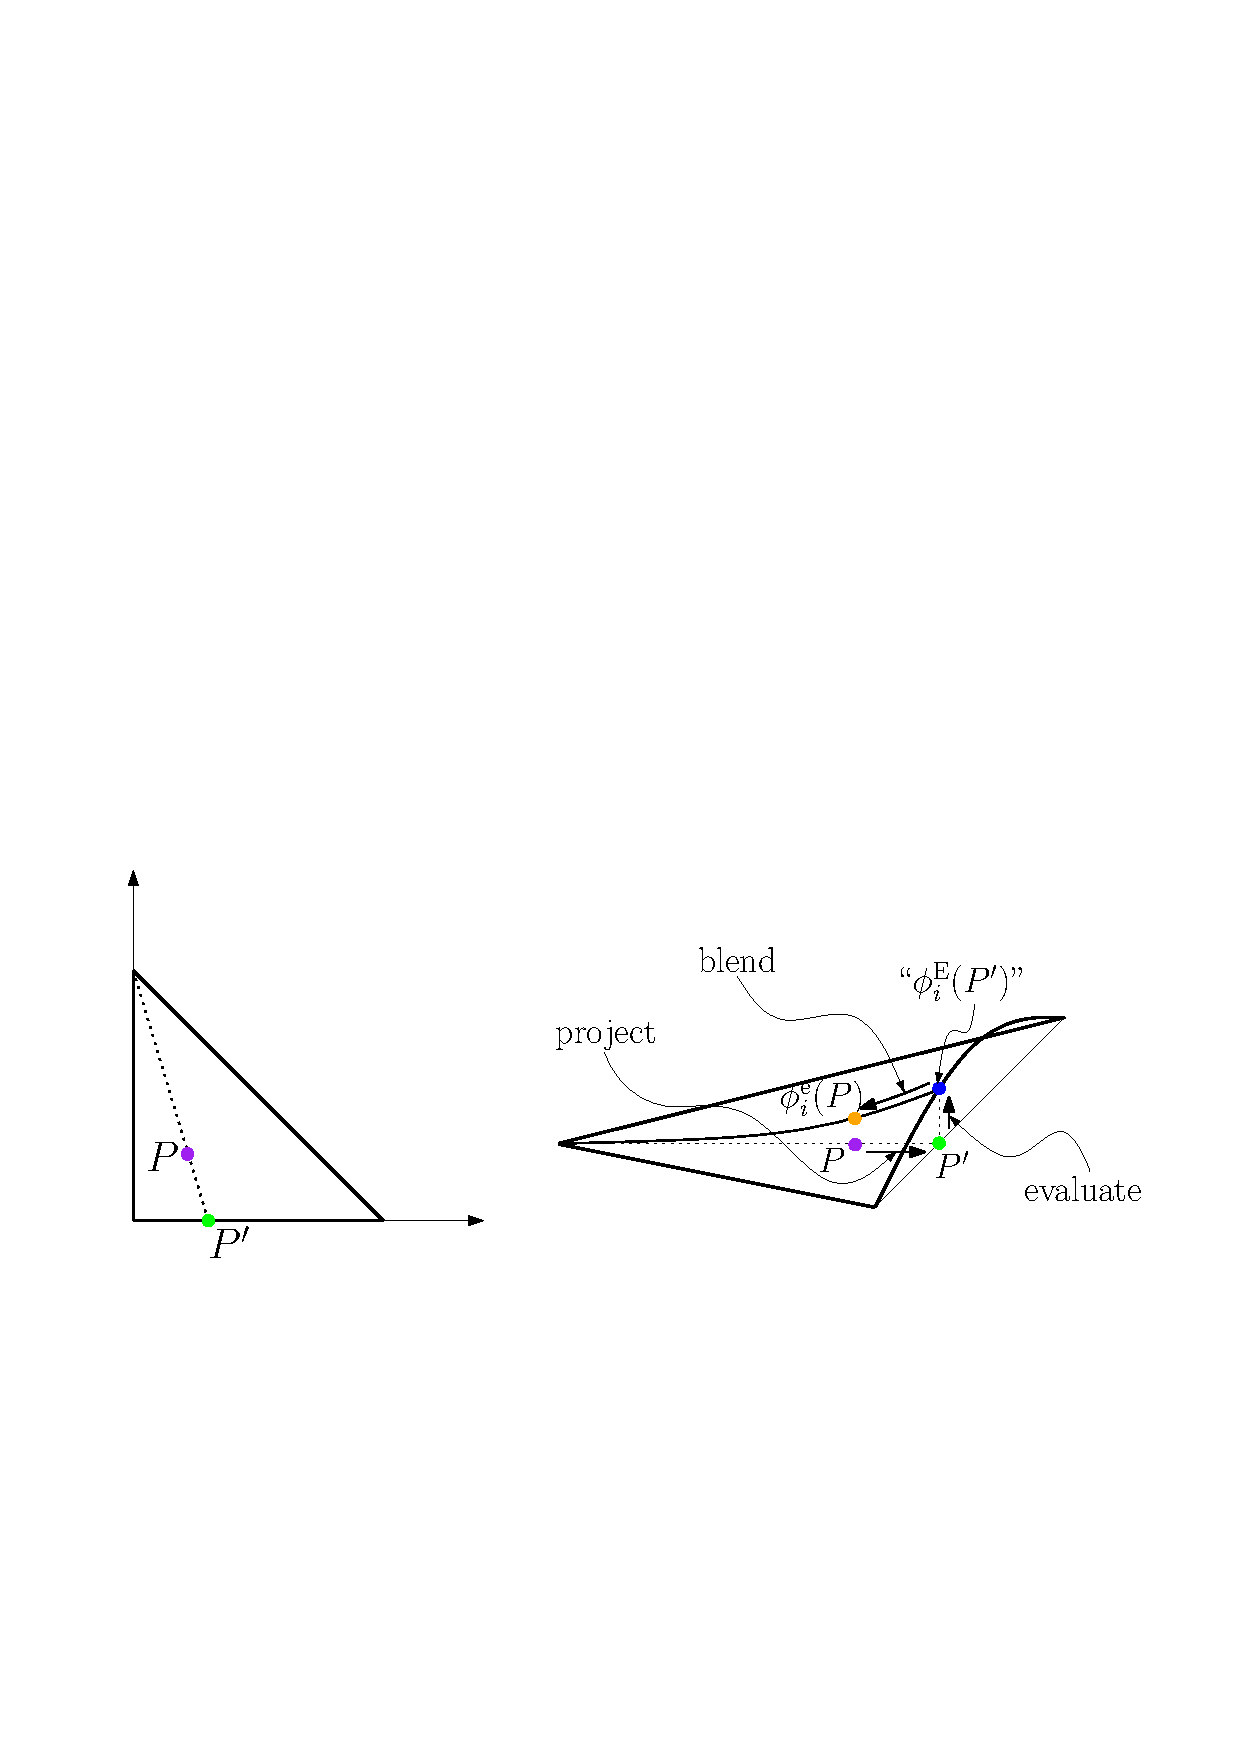
\includegraphics[scale=0.55]{./figures/TriangleProjection.pdf}
\caption{Edge projection from $P$ to $P'$, and the logic project$\,\to\,$evaluate$\,\to\,$blend.}
\label{fig:TriangleProjection}
\end{center}
\end{figure}

As with the quadrilateral, there is a geometrical interpretation to these expressions, and again it follows the fundamental logic of project$\,\to\,$evaluate$\,\to\,$blend, which is marked below:
\begin{equation*}
    \phi_i^\mathrm{e}(x)=\phi_i^\E(\vec{\nu}_{01}(x))
    	=\underbrace{(\nu_0(x)+\nu_1(x))^i}_{\text{blend}}
    		\underbrace{\phi_i^\E\Big(\underbrace{\textstyle{\frac{\nu_0(x)}{\nu_0(x)+\nu_1(x)}},
    			\textstyle{\frac{\nu_1(x)}{\nu_0(x)+\nu_1(x)}}}_{\text{project}}\Big)}_{\text{evaluate}}\,.
    				%=(\nu_0(x)+\nu_1(x))^i
    				%	[L_i]\Big(\textstyle{\frac{\nu_0(x)}{\nu_0(x)+\nu_1(x)}},\textstyle{\frac{\nu_1(x)}{\nu_0(x)+\nu_1(x)}}\Big)\,,
\end{equation*}
The coordinates $(\frac{\nu_0}{\nu_0+\nu_1},\frac{\nu_1}{\nu_0+\nu_1})$ are projected 1D coordinates, because they sum to $1$ for all $x$. 
Note this is \textit{not} true for the coordinates $(\nu_0,\nu_1)$ in general (only over the edge itself).
As argued before for the quadrilateral, the projected coordinates represent a point over edge 01:
\begin{equation*}
	(x_1,x_2)\;\longmapsto\;(\textstyle{\frac{x_1}{1-x_2}},0)\,.
\end{equation*}
Geometrically, it consists of finding the intersection $P'=(\frac{x_1}{1-x_2},0)$ of the edge with the projecting line passing through the original point $P=(x_1,x_2)$ and the disjoint opposite vertex. 
This projection and the logic of the construction is illustrated in Figure \ref{fig:TriangleProjection}.

%Note that in this case, the blending function is hiding within the homogenization process, and it is a \textit{nonlinear} function. Also, notice $\tilde{\mu}_1=\frac{\nu_1}{\nu_0+\nu_1}\in[0,1]$, since $\nu_1\geq0$ and $\nu_0\geq0$ by the properties of affine coordinates. Indeed, $\tilde{\mu}_1$ represents a projected coordinate. More explicitly, the two dimensional projection to edge 01 is
%\begin{equation*}
%	(x_1,x_2)\;\longmapsto\;(\textstyle{\frac{x_1}{1-x_2}},0)\,.
%\end{equation*}
%It consists of finding the intersection $P'=(\frac{x_1}{1-x_2},0)$ of the edge with the projecting line passing through the original point $P=(x_1,x_2)$ and the opposite vertex to the edge. This is illustrated in Figure \textit{add Figure}. Finally it is easy to check the desired trace properties:
%\begin{alignat*}{4}
%	&[L_i](\nu_0(x),\nu_1(x))|_{x_2=0}&&=[L_i](\mu_0(x_1),\mu_1(x_1))&&=L_i(x_1)\\
%	&[L_i](\nu_0(x),\nu_1(x))|_{x_2=1-x_1}&&=[L_i](0,x_1)&&=0\\
%	&[L_i](\nu_0(x),\nu_1(x))|_{x_1=0}&&=[L_i](1-x_1-x_2,0)&&=0\,.
%\end{alignat*}

%It should now be clear why $\phi_i^\E$ was defined so generally before in (\textit{put reference}). 
The complete list of edge functions with their gradients is
\begin{equation}
	\phi_i^\mathrm{e}(x)=\phi_i^\E(\vec{\nu}_{ab}(x))\,,\qquad\quad\nabla\phi_i^\mathrm{e}(x)=\nabla\phi_i^\E(\vec{\nu}_{ab}(x))\,,
	\label{eq:Triphigeneral}
\end{equation}
with $i=2,\ldots,p$, and $0\leq a<b\leq2$ (so $(a,b)=(0,1),(1,2),(0,2)$). As usual, there are a total of $p-1$ edge functions for every edge, for a total of $3(p-1)$ edge functions.
%
%\paragraph{Edge Orientations}
%To consider orientations, first look at the predefined local edge axis for a given edge, and replace $\phi_i^\E$ by $\phi_i^{\e,\oo}$ with the appropriate entries. 
%The oriented edge functions, which have supercript $\e,\oo$, are explained in \S\ref{sec:edgeorientations}.
%For example, take edge 01. 
%The predefined local edge axis $\xi^\mathrm{e}$ for this edge points from vertex 0 to vertex 1.
%This means the order of the entries in $\phi_i^{\e,\oo}$ is $(\nu_0(x),\nu_1(x))$ (and $\textit{not}$ $(\nu_1(x),\nu_0(x))$ which would apply if the local edge axis pointed from vertex 1 to vertex 0).
%This defines the $\oo=0$ orientation.
%Hence, for edge 12, \eqref{eq:Triphigeneral} becomes
%\begin{equation*}
%    \phi_i^\mathrm{e}(x)=\phi_i^{\e,\oo}(\nu_0(x),\nu_1(x))
%        =\begin{cases}
%            \phi_i^{\e,0}(\nu_0(x),\nu_1(x))
%            	=\phi_i^{\e}(\nu_0(x),\nu_1(x))\,\,\,&\text{if }\oo=0\\
%            \phi_i^{\e,1}(\nu_0(x),\nu_1(x))
%            	=\phi_i^{\e}(\nu_1(x),\nu_0(x))\,\,\,&\text{if }\oo=1\,,
%        \end{cases}
%\end{equation*}
%where \eqref{eq:orientEdge} was used as the definition of $\phi_i^{\e,\oo}$. The same applies to the gradients, and the other edge functions that follow in $H(\mathrm{curl})$ (which involve $E_i^\E$).
%

%We begin with a reintroduction of a construction of the 1D edge bubbles using affine coordinates. Let $p\geq2$ be the order of the edge and let $\hat\phi_i(t), t \in [0,1]$, be a polynomial of order $2\leq i\leq p$, vanishing at $t = 0,1$. Our default choice will be the shifted Lobatto polynomial,
%\be
%\hat\phi_i(t) = L_i(t) = L_i(t; 1) \, .
%\ee
%Introducing the affine edge coordinates:
%\be
%\mu_0 = 1 - t,\quad \mu_1 = t \, ,
%\ee
%we can represent function $\hat\phi_i$ in the form:
%\be
%\hat\phi_i(t) = \phi_i (\mu_0,\mu_1)
%\ee
%where function $\phi_i$ is a polynomial of (total) degree $i$
%in terms of the edge affine coordinates $\mu_0,\mu_1$. Given local affine coordinates $s_0,s_1$ of the $0-1$ edge (the construction is independent of the spatial dimension), we define the unoriented affine edge shape functions as:
%\be
%\phi^\E_i(s_0,s_1) = [\phi_i] (s_0,s_1) = \phi_i\left(\frac{s_0}{s_0+s_1},
%\frac{s_1}{s_0+s_1}\right) (s_0 + s_1)^i \, , \quad i=2,\ldots,p
%\label{eq:EdgeShap2}
%\ee
%where $p$ is the edge order.
%The map prescribing for a point in the triangle
%the corresponding point on the edge with edge coordinates:
%\be
%\mu_n = \frac{s_n}{s_0+s_1},\quad n=0,1\, ,
%\ee
%can be viewed as a projection onto the edge, whereas function
%$(s_0 + s_1)^i$ is the edge blending function.
%
%\begin{figure}[ht!]
%    \centering
%    \begin{subfigure}[b]{0.45\textwidth}
%        \includegraphics[width=\textwidth]{./figures/tri_V2.png}
%        \caption{Edge $H^1$ bubble for the triangle.}
%        \label{fig:H1edgebub_tri}
%    \end{subfigure}%
%\end{figure}
%    ~ %add desired spacing between images, e. g. ~, \quad, \qquad, \hfill etc.
%      %(or a blank line to force the subfigure onto a new line)
%    %\begin{subfigure}[b]{0.45\textwidth}
%    %    \includegraphics[width=\textwidth]{./tet_V2.png}
%    %    \caption{Edge $H^1$ bubble projection for the tet.}
%    %    \label{fig:H1edgebub_tet}
%    %\end{subfigure}
%    %\caption{Edge shape functions.}\label{fig:H1edgebub_tet}
%% \label{fig:H1bub_tri}
%%\end{figure}
%
%Contrary to the square or hexahedral element, the first term on the right hand side of Equation~\eqref{eq:EdgeShap2} {\em is not} a polynomial, however, the product {\em is}.
%As we will be using integrated polynomials $\left[L_i\right](\nu_1,\nu_0) = \phi^{\e}_i(\nu_0,\nu_1)$ we have that \begin{equation}\phi^{\e}_i(\nu_0,\nu_1)= \left[L_i\right](\nu_1,\nu_0) = L_i(\nu_0;\nu_0+\nu_1) \nonumber \end{equation}
%
%
%Moreover, it is not difficult to see that the edge shape function $\phi^\E_i(\nu_0,\nu_1)$ satisfies the required vanishing property. Indeed, by construction, $\phi^\E_i(\nu_0,\nu_1)$ is nonzero on the $0-1$ edge and zero on the other two edges. Also, $\nabla \phi^\E_i(\nu_0,\nu_1)$ lies in the proper N\'ed\'elec space.


%\paragraph{Orientation Considerations} We now consider the case where we have oriented edges, which, as we saw in the 1D case, was obtained by a simple permutation of the order of arguments in the shape function. In the triangle case, the situation is similar. Indeed, if we wish to consider the oriented case with orientation $\oo=1$, we {\em define} $\phi^{\e,\oo}_i(\nu_0,\nu_1) = \left[L_i\right](\nu_1,\nu_0) = L_i(\nu_0;\nu_0+\nu_1)$.
%With the above definition, we find that the set of $H^1$ edge shape functions on the $0-1$ edge for the triangle are given as
%\be
%\phi^{\e,\oo}_i(\nu_0,\nu_1) =
%\left\{
%    \begin{array}{ll}
%        \phi_i^{E}(\nu_0,\nu_1) = L_i(\nu_1;\nu_0+\nu_1) & \text{if } \oo = 0\\
%        \phi_i^{E}(\nu_1,\nu_0) = L_i(\nu_0;\nu_0+\nu_1) & \text{if } \oo = 1
%    \end{array}
%\right.
%\ee
%
%The full family of all edge shape functions for the triangle (and line segment) is composed of the shape functions above, $\phi^\E_i$, considered on each edge independently.
%% For simplicity, we have assumed unswapped coordinates in each case above.
%
%% We leave it as a simple excercise for the reader to show that if we allow for $i=1$ in the definiton~\eqref{eq:H1_CountingSimplexEdge}, then $\phi_1(s_k,s_l)$ agrees with the vertex shape functions defined previously, albeit with some overcounting in the case of the tetrahedron.
%% \textcolor{red}{Provide pictorial illustration of the projection in
%% both 2D and 3D.}
%
%
%% \textcolor{red}{Provide a pictorial example in 2D for an edge shape function}

\subsubsection{\texorpdfstring{$H^1$}{H1} Face Bubbles}

These intuitively involve all three affine coordinates $(\nu_0,\nu_1,\nu_2)$.% as opposed to only two of them (like the edges).
The first natural idea is to use the existing edge shape functions and multiply by another function $\hat{\phi}_j$ which vanishes at the remaining edge.
That is,
\begin{equation*}
	\phi_{ij}^\mathrm{f}(x)=\phi^\E_i(\nu_0(x),\nu_1(x))\hat{\phi}_j(\nu_2(x))\,.
\end{equation*}
Here, $\hat{\phi}_j(y)$ should also be an $H^1$ function with domain $y\in[0,1]$ (since $0\leq\nu_2(x)\leq1$) and which vanishes at $y=0$, so that $\hat{\phi}_j(0)=0$. 
Notice that in the quadrilateral, when constructing $\phi_{ij}^\Box$ the choice was naturally $\hat{\phi}_j=L_j$ since it was required that $\hat{\phi}_j(0)=\hat{\phi}_j(1)=0$, so it should vanish at \textit{both} endpoints. 
%Moreover, that case extends the pattern naturally to the hexahedron. 
For the triangle there is much more liberty for the choice of $\hat{\phi}_j$, and indeed it can be chosen such that it has many advantages. 
Following \citet{Beuchler_Schoeberl_06} it is chosen as a Jacobi polynomial, $\hat{\phi}_j=L_j^\alpha$, with $\alpha=2i$, where $i$ is the order of $\phi^\E_i$. This results in
\begin{equation*}
	\phi_{ij}^\mathrm{f}(x)=\phi^\E_i(\nu_0(x),\nu_1(x))L_j^{2i}(\nu_2(x))\,.
\end{equation*}

Thinking ahead to the tetrahedron, this definition can be easily generalized. Just as with $\phi_i^\E$, the generalization is nothing more than the homogenization of the previous formula, as written in \eqref{eq:homogproduct}.%As with edge to triangle, extension to tetrahedron, so more general definition next.

\begin{definition*}
Let $s_0$, $s_1$ and $s_2$ be arbitrary functions of some spatial variable in $\R^N$, with $N=2,3$, and denote by $p_s$ the order in the coordinate triplet $(s_0,s_1,s_2)$. Then
\begin{equation}
    \phi_{ij}^\Tri(s_0,s_1,s_2)=\phi_i^\E(s_0,s_1)[L_j^{2i}](s_0+s_1,s_2)=[L_i,L_j^{2i}](s_0,s_1,s_2)\,,
\end{equation}
for $i\geq2$, $j\geq1$ and $n=i+j=3,\ldots,p_s$. %$($or equivalently $i=n-j$, $j=1,\ldots,n-2$ and $n=i+j=3,\ldots,p$$)$. 
The gradients, understood in $\R^N$, are
\begin{equation}
    \begin{aligned}
    \nabla\phi_{ij}^\Tri(s_0,s_1,s_2)&=[L_j^{2i}](s_0+s_1,s_2)\nabla\phi_i^\E(s_0,s_1)
    	+\phi_i^\E(s_0,s_1)\nabla[L_j^{2i}](s_0+s_1,s_2)\,,
    \end{aligned}
\end{equation}
where for any $\alpha$,
\begin{equation}	
	\begin{aligned}
  	\nabla[L_j^\alpha](s_0\!+\!s_1,s_2)&=[P_{j-1}^\alpha](s_0\!+\!s_1,s_2)\nabla s_2
  		+[R_{j-1}^\alpha](s_0\!+\!s_1,s_2)\nabla(s_0\!+\!s_1\!+\!s_2)\\
        &=P_{j-1}^\alpha(s_2;s_0\!+\!s_1\!+\!s_2)\nabla s_2
        		+R_{j-1}^\alpha(s_2;s_0\!+\!s_1\!+\!s_2)\nabla(s_0\!+\!s_1\!+\!s_2)\,.
  \end{aligned}\label{eq:DerivativeofLalpha}
\end{equation}
\end{definition*}

% \be
% \phi^\f_{ij} = \phi^\E_i \left(\frac{\nu_0}{\nu_0+\nu_1},\frac{\nu_1}{\nu_0+\nu_1}\right)
% (\nu_0 + \nu_1)^i \, \hat\phi_j (\nu_2)
% \ee
%\be
%\phi^\Tri_{ij}(\nu_0,\nu_1,\nu_2) = \phi^\E_i \left(\nu_0,\nu_1\right) \hat\phi_j (\nu_2)
%\ee
%with
%$$
%i\ge2,\, j\ge1,\, i+j \leq p
%$$
%where $p$ is the order of the triangle and $\hat{\phi}_j(t),\,  t \in [0,1]$, is a polynomial of order $j$ vanishing at $t=0$.
%% Here $\phi^\E_i$ is an affine representation of a 1D $H^1$ bubble of order $i$, and polynomial $\hat{\phi}_j(x),\,  x \in [0,1]$, vanishes at $x=0$.
% Following Sven Beuchler and Joachim Sch\"{o}berl \textit{cite},
%we define \mbox{$\hat\phi_j := L^{2i-1}_{j}$}, the integrated shifted Jacobi polynomial with weight $\alpha = 2i-1$ and order $j$. In this case, we arrive at
%\be
%\begin{array}{ll}
%\phi^\Tri_{ij}(\nu_0,\nu_1,\nu_2) & = L_i(\frac{\nu_1}{\nu_0 + \nu_1}) (\nu_0 + \nu_1)^i L^{2i-1}_{j}(\nu_2)
%\\[8pt]
%& = L_i(\nu_1; \nu_0 + \nu_1) L^{2i-1}_{j}(\nu_2)
%\\[8pt]
%& = \left[L_i,L^{2i-1}_{j}\right](\nu_0,\nu_1,\nu_2)
%\end{array}
%\label{eq:H1_TriFace}
%\ee
%where in the final line we have used the property $\nu_0+\nu_1+\nu_2=1.$

%Again, we note that the vanishing property is satisfied by construction. The edge function $\phi^\E_i \left(\nu_0,\nu_1\right)$ vanishes on all edges except the $0-1$ edge, while the $H^1$ bubble $\hat\phi_j (\nu_2)$ vanishes when $\nu_2=0$, i.e., on the $0-1$ edge, so that the product, $\phi^\Tri_{ij}(\nu_0,\nu_1,\nu_2)$ vanishes on the entire boundary of the triangle, and is non-zero in the interior. Moreover, by a calculation entirely analogous to the edge case, the gradients of the face functions also lie in the appropriate space.
Note the indexing was shown as $i\geq2$, $j\geq1$ and $n=i+j=3,\ldots,p_s$. 
In many $hp$ codes it is useful to enforce hierarchy, so that the shape functions are organized by total order. 
That is, first list all order $3$ bubbles, then all order $4$ bubbles, and so on.
Hence when coding is in mind, it is useful to have an outer loop with numbering $n=3,\ldots,p_s$ and an inner loop indexing with either $i=2,\ldots,n-1$ (so $j=n-i$) or $j=1,\ldots,n-2$ (so $i=n-j$).

Regarding the vanishing properties of this new ancillary function, it suffices to rewrite \eqref{eq:LiLjvanishing} so that for any $s_0,s_1,s_2$, and all $i\geq2$, $j\geq1$,
\begin{equation}
	\phi_{ij}^\Tri(s_0,s_1,0)=\phi_{ij}^\Tri(s_0,0,s_2)=\phi_{ij}^\Tri(0,s_1,s_2)=0\,.\label{eq:phiTrivanishing}
\end{equation}

As expected, when the coordinates are 2D affine coordinates, the formulas for $\phi_{ij}^\Tri$ and its gradient are simplified.
For this, record the next remark.

\begin{remark}
Let $\nu_0=1-\nu_1-\nu_2$, where $\nu_1$ and $\nu_2$ are arbitrary functions of some spatial variable in $\R^N$, $N=2,3$, and where $p$ is the order in the coordinates $(\nu_0,\nu_1,\nu_2)$. Then for all $i\geq2$, $j\geq1$, and $n=i+j=3,\ldots,p$,
\begin{equation}
	\begin{aligned}
    \phi_{ij}^\Tri(\nu_0,\nu_1,\nu_2)&=\phi_i^\E(\nu_0,\nu_1)L_j^{2i}(\nu_2)\,,\\
    \nabla\phi_{ij}^\Tri(\nu_0,\nu_1,\nu_2)&=L_j^{2i}(\nu_2)\nabla\phi_i^\E(\nu_0,\nu_1)
    	+\phi_i^\E(\nu_0,\nu_1)P_{j}^{2i}(\nu_2)\nabla\nu_2\,.
	\end{aligned}
  \label{eq:H1Trispecialcase}
\end{equation}
\end{remark}


%Note the numbering was quoted as $i=n-j$, $j=1,\ldots,n-2$ and $n=3,\ldots,p$, which translates to $i\geq2$, $j\geq1$ and $n=i+j=3,\ldots,p$. The reason for this numbering is to enforce the idea that the triangle functions should be organized by total order. Hence, in a code the outer loop is in $n$, then $j$ and finally $i=n-j$ is fixed dependent on $n$ and $j$.  That is,
%\begin{verbatim}
%do n=3,...,p
%    do j=2,...,n-2
%        i=n-j
%        ...
%    enddo
%enddo
%\end{verbatim}
%Ensuring this hierarchy in total order is useful in many $hp$ codes.

%Also, observe that in two dimensions, where $\nu_0+\nu_1+\nu_2=1$, the formula collapses to the one proposed initially, while the formula for the gradients simplifies to
%\begin{align*}
%	\phi_{ij}^\Tri(\nu_0,\nu_1,\nu_2)&=L_j^{2i-1}(\nu_2)\nabla\phi_i^\E(\nu_0,\nu_1)
%		+\phi_i^\E(\nu_0,\nu_1)(P_{j-1}^{2i-1}(\nu_2;1)\nabla\nu_2+R_{j-1}^{2i-1}(\nu_2;1)\nabla1)\\
%			&=L_j^{2i-1}(\nu_2)\nabla\phi_i^\E(\nu_0,\nu_1)+\phi_i^\E(\nu_0,\nu_1)P_{j-1}^{2i-1}(\nu_2)\nabla\nu_2\,.
%\end{align*}

%The full family of all $H^1$ triangle face bubbles are simply the functions above, $\phi^\Tri
%_{ij}$. In this case orientations are not important and we need only construct one set of shape functions from blending a single family of edge shape functions (in this case, $\nu_2=0$);
%As usual, it is preferred to write all formulas in terms of $\phi_{ij}^\Tri$. This will be useful when orientations are introduced. 
In general, the $H^1$ triangle face bubbles and their gradients are
\begin{equation}
	\phi_{ij}^\mathrm{f}(x)=\phi_{ij}^\Tri(\vec{\nu}_{012}(x))\,,\qquad\quad
		\nabla\phi_{ij}^\mathrm{f}(x)=\nabla\phi_{ij}^\Tri(\vec{\nu}_{012}(x))\,,
% \phi^\f_{ij}(\nu_0,\nu_1,\nu_2)% = \left[L_i\right](s_k,s_l)
\label{eq:H1_CountingTriFace}
\end{equation}
where $i\geq2$, $j\geq1$ and $n=i+j=3,\ldots,p$. 
The vanishing conditions are satisfied by construction or simply by looking at \eqref{eq:phiTrivanishing}. 
There are a total of $\frac{1}{2}(p-1)(p-2)$ $H^1$ face bubbles for the triangle.

% \be
% \left\{\phi(x)\in\mathcal{P}^p(\hat\Delta) : \phi(x) = \phi^\f_{ij}(\nu_0(x),\nu_1(x),\nu_2(x))
% % \phi^\f_{ij}(\nu_0,\nu_1,\nu_2)% = \left[L_i\right](s_k,s_l)
%  \, , \quad i\ge2,\, j\ge1,\, i+j\leq p\right\}\,.
% \label{eq:H1_CountingTriFace}
% \ee

%\begin{remark}
%When coding, in order to enforce the hierarchy in the order of the shape functions, here and afterwards for other shape functions on simplices, construct a loop iterating in total order of the polynomial space. For example
%\begin{verbatim}
%do k=3,...,p
%    do j=1,...,p-2
%        i=k-j
%        ...
%    end
%end
%\end{verbatim}
%\end{remark}


%\paragraph{\texorpdfstring{$H^1$}{H1} Linear Independence}
%
%To account for all of the constructed shape functions for the triangle, we set $d=2$ and sum all of the shape functions constructed in Equations~\eqref{eq:H1_CountingSimplexVert}, \eqref{eq:H1_CountingSimplexEdge}, and \eqref{eq:H1_CountingTriFace}:
%\be
%3+3(p-1)+{p-1\choose 2} = {p+2\choose 2}
%\ee
%which is equal to the dimension of $\mathcal{P}^p$ for $d=2$.
%The linear independence of the above shape functions, using the presented Lobatto and integrated Jacobi polynomials is given for the triangle in \textit{cite Beuchler} and \textit{cite}.
%
%Since the cardinality of our set of linearly independent shape functions agrees with the dimension of $\mathcal{P}^p$ for both the triangle, we understand that our set is spanning and that we have constructed an appropriate basis for the space.

\subsection{\texorpdfstring{$H(\mathrm{curl})$}{Hcurl} Shape Functions}

%As a reminder, in two dimensions, the trace of $H(\mathrm{curl})$ functions is the tangential component of the vector function along the boundary (that is, the edges).
%Hence, all edge functions should have vanishing trace at all other edges, while the bubbles should have zero trace at all edges. 

The dimension of $\mathcal{N}^p$ in two dimensions is $p(p+2)$.
A careful count of the linearly independent conforming shape functions to be presented throughout this section will coincide with that dimension. 
Showing that the functions constructed are in $\mathcal{N}^p$ is nontrivial, but will follow from the next instrumental lemma.% where one must recall the definition of $H(\mathrm{curl})$ edge functions in \eqref{eq:Hcurledgefunctions}.

\begin{lemma}
\label{lemma:curl}
Let $x\in\R^N$ for $N=2,3$, and $f_n\in\mathcal{P}^n(x)$ be any polynomial of total order $n$ in the coordinates $x=(x_1,\ldots,x_N)$. Given $s_0$ and $s_1$ coordinates in $\mathcal{P}^1(x)$ $($linear functions in $x$$)$, it follows that the N\'ed\'elec space of order $n+1$, $\mathcal{N}^{n+1}$, contains the function
\begin{equation*}
	f_n(\bcdot)\Big(s_0\nabla s_1-s_1\nabla s_0\Big)\in\mathcal{N}^{n+1}\,.
\end{equation*}
\end{lemma}
\begin{proof}
Recall the definition of the N\'ed\'elec space,
\begin{equation*}
	\mathcal{N}^p=(\mathcal{P}^{p-1})^N\oplus\Big\{E\in(\tilde{\mathcal{P}}^{p})^N: x\cdot E(x)=0\,\text{ for all } 
		x\in\R^N\Big\}\,.
\end{equation*}
The (affine) coordinates are linear functions in $x=(x_1,\ldots,x_N)$, so that
\begin{equation*}
	s_k(x)=a_k+b_k\cdot x\,,
\end{equation*}
for $a_k\in\R$, $b_k\in\R^N$ and $k=0,1$. As a result $\nabla s_k(x)=b_k$, and
\begin{equation*}
	s_0(x)\nabla s_1(x)-s_1(x)\nabla s_0(x)=\underbrace{(a_0b_1-a_1b_0)}_{=A}+\underbrace{((b_0\cdot x)b_1-(b_1\cdot x)b_0)}_{=B(x)}\,.
\end{equation*}
Clearly, $A\in(\mathcal{P}^0)^N=\R^N$, while $B\in(\tilde{\mathcal{P}}^1)^N$. Moreover,
\begin{equation*}
	x\cdot B(x)=x\cdot((b_0\cdot x)b_1-(b_1\cdot x)b_0)=(b_0\cdot x)(b_1\cdot x)-(b_1\cdot x)(b_0\cdot x)=0\,,
\end{equation*}
so that $B\in\{E\in(\tilde{\mathcal{P}}^{1})^N: x\cdot E(x)=0\}$, and $s_0\nabla s_1-s_1\nabla s_0\in\mathcal{N}^1$.

Now, $f_n\in\mathcal{P}^n=\mathcal{P}^{n-1}\oplus\tilde{\mathcal{P}}^n$, for $n\geq1$ can always be decoupled into $f_n=f_{n-1}+\tilde{f}_n$, where $f_{n-1}\in\mathcal{P}^{n-1}$ and $\tilde{f}_n\in\tilde{\mathcal{P}}^n$. As a result
\begin{equation*}
	f_n(x)(s_0(x)\nabla s_1(x)-s_1(x)\nabla s_0(x))=f_n(x)A+f_{n-1}(x)B(x)+\tilde{f}_n(x)B(x)\,,
\end{equation*}
where it is clear $f_{n}A+f_{n-1}B\in(\mathcal{P}^n)^N$ and $\tilde{f}_nB\in(\tilde{\mathcal{P}}^{n+1})^N$. Meanwhile, 
\begin{equation*}
x\cdot(\tilde{f}_n(x)B(x))=\tilde{f}_n(x)x\cdot B(x)=0\,.
\end{equation*}
Hence, $f_n(\bcdot)(s_0\nabla s_1-s_1\nabla s_0)\in\mathcal{N}^{n+1}$.
\end{proof}



%\begin{proof}\,
%We begin with the observation that the homogenization operation
%\be
%[\cdot]:\mathcal{P}^n\to\tilde{\mathcal{P}^n}
%\ee
%is surjective. In this case, any monomial in $f_n\in\tilde{\mathcal{P}^n}$ may be expressed as
%\be
%f_n(s_0,s_1) = g_n\left(\frac{s_0}{s_0+s_1},\frac{s_1}{s_0+s_1}\right)\left(s_0+s_1\right)^n,
%\ee
%for some $g_n\in\mathcal{P}^n$. We now see, by direct computation, that
%\begin{align*}
%\bfnab\times E(s_0,s_1) &= \bfnab\times \left(f_n(s_0,s_1) [s_0 \bfnab s_1 - s_1 \bfnab s_0 ]\right)\\
%&= \bfnab \left(g_n\left(\frac{s_0}{s_0+s_1},\frac{s_1}{s_0+s_1}\right)\left(s_0+s_1\right)^n\right) \times [s_0 \bfnab s_1 - s_1 \bfnab s_0 ] + f_n(s_0,s_1) \bfnab\times [s_0 \bfnab s_1 - s_1 \bfnab s_0 ]\\
%&= \bfnab g_n\left(\frac{s_0}{s_0+s_1},\frac{s_1}{s_0+s_1}\right)\left(s_0+s_1\right)^n \times [s_0 \bfnab s_1 - s_1 \bfnab s_0 ]\\
%&\quad + g_n\left(\frac{s_0}{s_0+s_1},\frac{s_1}{s_0+s_1}\right) n \left(s_0+s_1\right)^{n-1}\left(\bfnab s_0 + \bfnab s_1\right) \times [s_0 \bfnab s_1 - s_1 \bfnab s_0 ] \\
%&\quad + 2f_n(s_0,s_1) \bfnab s_0 \times \bfnab  s_1\\
%&= (n+2) \, f_n(s_0,s_1) \, \bfnab s_0 \times \bfnab  s_1 \, ,
%\end{align*}
%since
%\be
%\bfnab g_n\left(\frac{s_0}{s_0+s_1},\frac{s_1}{s_0+s_1}\right) \quad \parallel \quad [s_0 \bfnab s_1 - s_1 \bfnab s_0 ] \, .
%\ee
%
%Now, let $x = (x_1,\ldots,x_N)\in\hat\Delta$ be the Cartesian coordinates of $x$. Then,
%\be
%s_k = a_k + \sum_{i=1}^Nb_{ki}x_i,
%\ee
%where $a_k,b_{ki}\in\mathbb{R}$, $k=1,2$, $i=1,\ldots,N$. Since each $s_k$ is an affine function, $s_0 \bfnab s_1 - s_1 \bfnab s_0 \in \left(\mathcal{P}^{1}\right)^d$. Moreover, letting $\{\bfe_i\}_{i=1}^N$ be the Euclidean basis,
%\be
%s_0 \bfnab s_1 - s_1 \bfnab s_0 = \sum_{i=1}^N\left(a_0 b_{1i}-a_1 b_{0i}\right)\bfe_i + \sum_{i,j=1}^N\left( b_{0i}b_{1j}-b_{1i}b_{0j}\right)x_i\bfe_j,
%\ee
%where
%\be
%%a_0\sum_{i=1}^N b_{1i}\bfe_i-a_1\sum_{i=1}^N b_{0i}\bfe_i
%\sum_{i=1}^N\left(a_0 b_{1i}-a_1 b_{0i}\right)\bfe_i \in \left(\mathcal{P}^0\right)^d,
%\ee
%and
%\be
%%\left(\sum_{i=1}^N b_{0i}x_i\right)\left(\sum_{i=1}^N b_{1i}\bfe_i\right)-\left(\sum_{i=1}^N b_{1i}x_i\right)\left(\sum_{i=1}^N b_{0i}\bfe_i\right)
%\sum_{i,j=1}^N\left( b_{0i}b_{1j}-b_{1i}b_{0j}\right)x_i\bfe_j \in \left(\tilde{\mathcal{P}}^1\right)^d.
%\ee
%Moreover,
%\be
% x \cdot \sum_{i,j=1}^N\left( b_{0i}b_{1j}-b_{1i}b_{0j}\right)x_i\bfe_j = \sum_{i,j=1}^N\left( b_{0i}b_{1j}-b_{1i}b_{0j}\right)x_ix_j = 0.
%\ee
%Therefore,
%\be
%s_0 \bfnab s_1 - s_1 \bfnab s_0 \in \mathcal{N}^1,
%\ee
%and the general result follows.
%
%\end{proof}

\subsubsection{\texorpdfstring{$H(\mathrm{curl})$}{Hcurl} Edges}

Having seen what ocurred with $H^1$ edge functions due to the process of homogenization, it is wise to consider the general definition of $H(\mathrm{curl})$ edge functions in \eqref{eq:Hcurledgefunctions}, using 2D affine coordinates as entries. 
Indeed this will suffice.
For instance, for edge 01, the shape functions are
\begin{equation*}
	\begin{aligned}
		E_i^\mathrm{e}(x)&=E_i^\E(\vec{\nu}_{01}(x))=[P_i](\vec{\nu}_{01}(x))\Big(\nu_0(x)\nabla\nu_1(x)-\nu_1(x)\nabla\nu_0(x)\Big)\\
    	&=(\nu_0(x)+\nu_1(x))^i
    		[P_i]\Big(\textstyle{\frac{\nu_0(x)}{\nu_0(x)+\nu_1(x)}},\textstyle{\frac{\nu_1(x)}{\nu_0(x)+\nu_1(x)}}\Big)
    			E_0^\E(\vec{\nu}_{01}(x))\\
    	&=\underbrace{(\nu_0(x)+\nu_1(x))^{i+2}}_{\text{blend}}
    		\underbrace{E_i^\E\Big(\underbrace{\textstyle{\frac{\nu_0(x)}{\nu_0(x)+\nu_1(x)}},
    			\textstyle{\frac{\nu_1(x)}{\nu_0(x)+\nu_1(x)}}}_{\text{project}}\Big)}_{\text{evaluate}}\,,
	\end{aligned}
\end{equation*}
for $i=0,\ldots,p-1$. 
By Lemma \ref{lemma:curl} it easily follows $E_i^\mathrm{e}\in\mathcal{N}^{i+1}\subseteq\mathcal{N}^{p}$ as desired.
The tangential trace properties are also satisfied. 
To see this, it suffices to look at $E_0^\mathrm{e}$, since $E_i^\mathrm{e}(x)=[P_i](\vec{\nu}_{01}(x))E_0^\mathrm{e}(x)$. 
Its traces are
\begin{alignat*}{3}
    &\mathrm{tr}(E_0^\mathrm{e}(x))|_{x_2=0}&&=E_0^\E(\vec{\nu}_{01}(x))|_{\nu_2=0}\cdot(v_1-v_0)
    	=\nabla\nu_1(x)\cdot(v_1-v_0)=1\,,\\
    &\mathrm{tr}(E_0^\mathrm{e}(x))|_{1-x_1-x_2=0}&&=E_0^\E(\vec{\nu}_{01}(x))|_{\nu_0=0}\cdot(v_2-v_1)
    	=-\nu_1(x)\nabla\nu_0(x)\cdot(v_2-v_1)=0\,,\\
  	&\mathrm{tr}(E_0^\mathrm{e}(x))|_{x_1=0}&&=E_0^\E(\vec{\nu}_{01}(x))|_{\nu_1=0}\cdot(v_2-v_0)
  		=\nu_0(x)\nabla\nu_1(x)\cdot(v_2-v_0)=0\,.
\end{alignat*}
Here the vanishing traces follow from the fact that the gradient of a function is always perpendicular to the tangents of its isosurfaces. 
Hence $\nabla\nu_0(x)$ is perpendicular to the tangents of the set where $\nu_0(x)=0$, which is precisely where $v_2-v_1$ lies. 
Regarding the nonzero trace, the formula $\nabla\nu_1(x)\cdot(v_1-v_0)$ follows after replacing $\nu_0=1-\nu_1$, and noting that $\nabla(\nu_0(x)+\nu_1(x))\cdot(v_1-v_0)=-\nabla\nu_2(x)\cdot(v_1-v_0)=0$.

More generally, the edge functions and their curls are
\begin{equation}
	E_i^\mathrm{e}(x)=E_i^\E(\vec{\nu}_{ab}(x))\,,\qquad\quad\nabla\times E_i^\mathrm{e}(x)=\nabla\times E_i^\E(\vec{\nu}_{ab}(x))\,,
	\label{eq:TriEgeneral}
\end{equation}
with $i=0,\ldots,p-1$, and $0\leq a<b\leq2$ (so $(a,b)=(0,1),(1,2),(0,2)$). There are a total of $p$ edge functions for every given edge, giving a total of $3p$ edge functions.
%It can also be readily checked that the desired trace properties are satisfied. 
%That is, the (tangential) trace is of the form $P_{i}(x_a)$ for some $a=1,2$ over edge $ab$ and zero over the other two edges.
%Moreover, by Lemma \ref{lemma:curl} it easily follows $E_i^\mathrm{e}\in\mathcal{N}^{i+1}$ for all $i=0,\ldots,p-1$.





%Consider the $0-1$ edge of the triangle and let $p$ be the order of this edge. In unlike the $H^1$ case, in $H(\text{curl})$ we no longer need an endpoint vanishing property for the edge shape functions. % Ultimately, the shape of shape functions restricted to a given edge should conform to $??(\marhbb{R})$ instead of $H^{1/2}(\mathbb{R})$.
%Given the have a larger space of polynomials available to us (one without endpoint conditions), we describe a new notation: let $\hat\psi_i\in\mathcal{P}^{p-1}$ be any given polynomial of order $i\leq p-1$.
%
%Without taking into account embedded orienations, for an edge with endpoint affine coordinates $\nu_0,\nu_1$, we define the affine $H(\text{curl})$ edge functions by:
%\be
%E^\E_i(\nu_0,\nu_1) = \left[\hat\psi_i\right](\nu_0,\nu_1)
%(\nu_0 \bfnab \nu_1 - \nu_1 \bfnab \nu_0 )\, , \quad i=0,\ldots,p-1\,.
%\label{eq:edge_curl}
%\nonumber
%\ee
%If $\hat\psi_i = P_i$, where $P_i$ denotes the shifted scaled Legendre polynomial of order $i$, then clearly, $$\left[\hat\psi_i\right] = \left[P_i\right]\,,$$
%\be
%E^{e}_i(x_1,x_2)= E^\E_i(\nu_0,\nu_1) = \left[P_i\right](\nu_0,\nu_1)
%(\nu_0 \bfnab \nu_1 - \nu_1 \bfnab \nu_0 )\, , \quad i=0,\ldots,p-1\,.
%\label{eq:edge_curl_1}
%\nonumber
%\ee
%and by Lemma~\ref{lemma:curl},
%\be
%\bfnab \times E_i^\E(\nu_0,\nu_1) =  (i+2) \, \left[P_i\right](\nu_0,\nu_1) \,
%\bfnab \nu_0 \times \bfnab \nu_1 \, .
%\nonumber
%\ee
%Note that for $i=0$ we obtain the Whitney edge functions and all functions live in the Ned\'{e}l\'{e}c space of ``order'' $i + \half$,
%\be
%E^\mathrm{e}_i \in \mathcal{N}^i\,.
%\ee
%Note also that in general, we have the following formula for the edge shape functions:
%
%\be
%E^{e}_i(x_1,x_2) = E^\E_i(\nu_a,\nu_b) = \left[P_i\right](\nu_a,\nu_b)
%(\nu_a \bfnab \nu_b - \nu_b \bfnab \nu_a )\, , \quad i=0,\ldots,p-1\,,
%\label{eq:edge_curl_2}
%\nonumber
%\ee
%where $a,b = 0,1,2$ and $a\leq b$
%\paragraph{Orientation Consideration}
%
%Taking into account orientation changes on the edge, as before we have the following orientation embedded definitons for the affine $H(\text{curl})$ edge functions
%\be
%E^{\e,\oo}_i(\nu_0,\nu_1) =
%\left\{
%    \begin{array}{ll}
%        \left[P_i\right](\nu_0,\nu_1)\left(\nu_0 \bfnab \nu_1 - \nu_1 \bfnab \nu_0\right) & \text{if } \oo =0 \\
%        \left[P_i\right](\nu_1,\nu_0)\left(\nu_1 \bfnab \nu_0 - \nu_0 \bfnab \nu_1\right) & \text{if } \oo =1
%    \end{array}
%\right.
%\ee
%for the triangle.

\subsubsection{\texorpdfstring{$H(\mathrm{curl})$}{Hcurl} Face Bubbles}

The construction of $H(\mathrm{curl})$ face bubbles is parallel to that of $H^1$ bubbles. 
The idea is to multiply $H(\mathrm{curl})$ edge functions with an $H^1$ function vanishing at zero. 
%Again, there is some liberty in the choice of the $H^1$ function. 
Again, it is chosen according to \citet{Beuchler_Pillwein_Zaglmayr_13} as the Jacobi polynomial, $L_j^\alpha$, with $\alpha=2i+1$, where $i$ is the order of $E^\E_i$.
Like the quadrilateral, the triangle has two closely related families generated by the same ancillary operator defined below.
%In fact there are two closely related families.
%They are defined generally below.

\begin{definition*}
Let $s_0$, $s_1$ and $s_2$ be arbitrary functions of some spatial variable in $\R^N$, with $N=2,3$, and denote by $p_s$ the order in the coordinate triplet $(s_0,s_1,s_2)$. Then
\begin{equation}
    E_{ij}^\Tri(s_0,s_1,s_2)=[L_j^{2i+1}](s_0+s_1,s_2)E_i^\E(s_0,s_1)\,,
\end{equation}
for $i\geq0$, $j\geq1$ and $n=i+j=1,\ldots,p_s-1$.
%$i=n-j$, $j=1,\ldots,n$ and $n=1,\ldots,p-1$ $($or equivalently $i\geq0$, $j\geq1$ and $n=i+j=1,\ldots,p-1$$)$. 
The curls, understood in $\R^N$, are
\begin{equation}
    \begin{aligned}
    \nabla\!\times\! E_{ij}^\Tri(s_0,s_1,s_2)&\!=\![L_j^{2i+1}](s_0\!+\!s_1,s_2)\nabla\!\times\! E_i^\E(s_0,s_1)
    	\!+\!\nabla[L_j^{2i+1}](s_0\!+\!s_1,s_2)\!\times\! E_i^\E(s_0,s_1)\,,
    \end{aligned}
\end{equation}
where $\nabla[L_j^{2i+1}](s_0+s_1,s_2)$ is computed from \eqref{eq:DerivativeofLalpha}.
%Also,
%\begin{equation}
%    \begin{aligned}
%    E_{ij}^{\Delta_{II}}(s_0,s_1,s_2)&=E_{ij}^{\Delta_{I}}(s_1,s_2,s_0)\,,\qquad\quad
%    	\nabla\times E_{ij}^{\Delta_{II}}(s_0,s_1,s_2)=\nabla\times E_{ij}^{\Delta_{I}}(s_1,s_2,s_0)\,,
%    \end{aligned}
%\end{equation}
%for $i=n-j$, $j=1,\ldots,n$ and $n=1,\ldots,p-1$ $($or equivalently $i\geq0$, $j\geq1$ and $n=i+j=1,\ldots,p-1$$)$.
\end{definition*}

As with the edge functions, it is clear that when evaluated in any permutation of $(\nu_0,\nu_1,\nu_2)$ the vanishing trace properties are satisfied.
The two families defined below give a total of $p(p-1)$ $H(\mathrm{curl})$ triangle face bubbles (each family has $\frac{1}{2}p(p-1)$).
%In view of this, each family has $\frac{1}{2}p(p-1)$, so that there is a total of $p(p-1)$ $H(\mathrm{curl})$ triangle face bubbles. 
%In both families the vanishing properties are satisifed by construction.

\subparagraph{Family I:} 
The shape functions for the first family and their curl are
\begin{equation}
	E_{ij}^{\mathrm{f}}(x)=E_{ij}^\Tri(\vec{\nu}_{012}(x))\,,\qquad\quad
		\nabla\times E_{ij}^{\mathrm{f}}(x)=\nabla\times E_{ij}^\Tri(\vec{\nu}_{012}(x))\,,
\end{equation}
for $i\geq0$, $j\geq1$ and $n=i+j=1,\ldots,p-1$. 
By Lemma \ref{lemma:curl}, $E_{ij}^\mathrm{f}\in\mathcal{N}^{n+1}$, where $n=i+j$. 
There are $\frac{1}{2}p(p-1)$ bubble functions in this family.
%The vanishing properties can be readily checked. There are $\frac{1}{2}p(p-1)$ $H(\mathrm{curl})$ face bubbles in this family.

\subparagraph{Family II:}
The shape functions for the second family and their curl are
\begin{equation}
	E_{ij}^{\mathrm{f}}(x)=E_{ij}^\Tri(\vec{\nu}_{120}(x))\,,\qquad\quad
		\nabla\times E_{ij}^{\mathrm{f}}(x)=\nabla\times E_{ij}^\Tri(\vec{\nu}_{120}(x))\,,
\end{equation}
for $i\geq0$, $j\geq1$ and $n=i+j=1,\ldots,p-1$.
The only difference with the first family is that the entries are permuted to $\vec{\nu}_{120}(x)=(\nu_1(x),\nu_2(x),\nu_0(x))$ instead of $\vec{\nu}_{012}(x)=(\nu_0(x),\nu_1(x),\nu_2(x))$.
Again, they lie in $E_{ij}^\mathrm{f}\in\mathcal{N}^{n+1}$, where $n=i+j$, and there are $\frac{1}{2}p(p-1)$ bubble functions in this family.

%Let $p$ be the order of the triangle face and
%$$i \geq 0,\, j \geq 1,\quad i+j=1,\ldots,p-1\,.$$
%
%Continuing the logic of the construction of affine $H^1$ triangle bubbles and edge $H(\text{curl})$ functions, we define the {\em first family} of triangle $H(\text{curl})$ bubbles as follows:
%\be
%E^\mathrm{f}_{ij}(x) = E^\Tri_{ij}(\nu_0(x),\nu_1(x),\nu_2(x))\,,
%\ee
%where
%\begin{align}
%E^\Tri_{ij}(\nu_0,\nu_1,\nu_2) &= E^\E_{i}(\nu_0,\nu_1) \, L^{2i-1}_{j}(\nu_2)
%\nonumber\\
%& = \left[P_i,L^{2i-1}_{j}\right](\nu_0,\nu_1,\nu_2)(\nu_0 \bfnab \nu_1 - \nu_1 \bfnab \nu_0 )\, .
%\label{eq:Hcurl_Face1}
%\end{align}
%In the above equation we recall that $E^\E_{i}$ is the $H(\text{curl})$ edge shape function corresponding to the first triangle edge, see (), and $L^{2i-1}_{j}$ denotes the shifted integrated Jacobi polynomial with weight $2i-1$ and order $j$.
%%\ref{eq:edge_curl}
%This motivates the the following definition for a generic function. Given arguments $s_0,s_1,s_2$ of a simplex (triangle, tetrahedron), we define the following two sets of {$H(\text{curl})$} triangle bubbles.
%
%\begin{definition*} Given the bubble function $E^\Tri_{ij}(s_0(x),s_1(x),s_2(x))$ with arguments $s_0(x),s_1(x),s_2(x)$, the corresponding two sets of $H(\text{curl})$ triangle bubbles are: \\$E^{\Delta_I}_{ij}(s_0(x),s_1(x),s_2(x)) = E^\Tri_{ij}(s_0(x),s_1(x),s_2(x)) \\
%E^{\Delta_II}_{ij}(s_0(x),s_1(x),s_2(x)) = E^\Tri_{ij}(s_1(x),s_2(x),s_0(x))$ \\
%where $E^\Tri_{ij}(s_0(x),s_1(x),s_2(x)) =  \left[P_i,L^{2i-1}_{j}\right](s_0(x),s_1(x),s_2(x))(s_0 \bfnab s_1 - s_1 \bfnab s_0 )$
%\\\end{definition*}

% Above,
% $$
% \bfnab L^{2i-1}_{j}(\nu_2) = \frac{d L^{2i-1}_{j}}{dx} (\nu_2)
% \, \bfnab \nu_2 = P^{2i-1}_{j-1} (\nu_2)
% \, \bfnab \nu_2\, .
% $$
%The above definition, as applied to the case of affine coordinates yields two sets of triangle bubbles, one set of triangle bubbles is constructed by rotating the indices of the other\footnote{Only one rotation of the indices is required to span this space}.

%\begin{description}
%  \item[Family I:]
%\be
%E^\mathrm{f}_{ij}(x) = E^\Tri_{ij}(\nu_0(x),\nu_1(x),\nu_2(x)),\quad i \geq 0,\, j \geq 1,\quad i+j=1,\ldots,p-1
%\ee
%
%  \item[Family II:]
%\be
%E^\mathrm{f}_{ij}(x) = E^\Tri_{ij}(\nu_1(x),\nu_2(x),\nu_0(x)),\quad i \geq 0,\, j \geq 1,\quad i+j=1,\ldots,p-1\,.
%\ee
%
%\end{description}


%\paragraph{\boldmath{$H(\text{curl})$} Linear Independence}
%
%Note that for the triangle, we have
%\be
%3p+2{p\choose 2} = p(p+2)
%\ee
%shape functions.


\subsection{\texorpdfstring{$H(\mathrm{div})$}{Hdiv} Shape Functions}
\label{sec:TriangleHdiv}

In two dimensions, the $H(\mathrm{div})$ space (see \eqref{eq:Hdiv2Ddef}) is isomorphic to $H(\mathrm{curl})$. 
%Indeed, this is achieved simply by rotating the $H(\mathrm{curl})$ functions. 
Indeed, just like with the quadrilateral, given a shape function $E\in H(\mathrm{curl})$ and its curl $\nabla\times E\in L^2$, the corresponding $H(\mathrm{div})$ shape function with its divergence is
\begin{equation}
    V=\begin{pmatrix}0&1\\-1&0\end{pmatrix}E\,,\quad\qquad\nabla\cdot V=\nabla\times E\,.
\end{equation}
Although not immediate, note that in \textit{two} dimensions the original polynomial space $\mathcal{N}^p$ for $H(\mathrm{curl})$ simply becomes the $H(\mathrm{div})$ conforming space $\mathcal{RT}^p$ after the rotation, as required.


\subsection{\texorpdfstring{$L^2$}{L2} Shape Functions}

These span $\mathcal{P}^{p-1}$, so there should be $\frac{1}{2}p(p+1)$ linearly independent shape functions.

\subsubsection{\texorpdfstring{$L^2$}{L2} Face}

%Analagous to the construction of the $H^1$ triangle bubbles, we use homogenization to construct the $L^2$-conforming shape functions for the triangle. In this case, the arguments have no special continuity properties for traces, and we define
Again, carefully chosen Jacobi polynomials are present in this construction. 
%The former ensures that the shape functions lie in $\mathcal{P}^{p-1}$, as required.
The shape functions are
\begin{equation}
\begin{aligned}
	\psi_{ij}^\mathrm{f}(x)&=[P_i](\nu_0(x),\nu_1(x))[P_j^{2i+1}](\nu_0(x)+\nu_1(x),\nu_2(x))\\
		&=[P_i,P_j^{2i+1}](\vec{\nu}_{012}(x))(\nabla\nu_1(x)\!\!\times\!\!\nabla\nu_2(x))\,,
\end{aligned}
\end{equation}
where $i\geq0$, $j\geq0$ and $n=i+j=0,\ldots,p-1$.
%$i=n-j$, $j=0,\ldots,n$ and $n=0,\ldots,p-1$ (or equivalently $i\geq0$, $j\geq0$ and $n=i+j=0,\ldots,p-1$). 
Clearly the functions lie in $\mathcal{P}^{p-1}$ and there are $\frac{1}{2}p(p+1)$ such functions. 
The factor $\nabla\nu_1(x)\!\times\!\nabla\nu_2(x)$ makes the expression coordinate free (with the $x$ coordinates it is $1$).
%$$
%i,j \geq 0,\quad i+j=0,\ldots,p-1 \, .
%$$

%\paragraph{\texorpdfstring{$L^2$}{L2} Linear Independence}
%
%In this final space, we clearly have
%\be
%{p+1\choose2}
%\ee
%shape functions for the triangle.
%
%The verification that we have constructed a basis follows similarly from the $H^1$ case.

\subsection{Orientations}
\label{sec:TriaOrientations}

Only edge orientations are required to ensure compatibility of 2D triangles.
However, in 3D elements, triangle \textit{faces} have the notion of orientation, and one needs to consider this to ensure full compatibility.
In \S\ref{sec:QuadEdgeOrientations} it was shown how to apply the principles introduced in \S\ref{sec:edgeorientations} to construct orientation embedded edge functions.
It is convenient to have read those sections.
In what follows, a brief illustration of how it analogously applies to the triangle is given in \S\ref{sec:TriaEdgeOrientations}.
Afterwards, in \S\ref{sec:TriaFaceOrientations}, the triangle face orientations are described.

\subsubsection{Edge Orientations}
\label{sec:TriaEdgeOrientations}

\begin{figure}[!ht]
\begin{center}
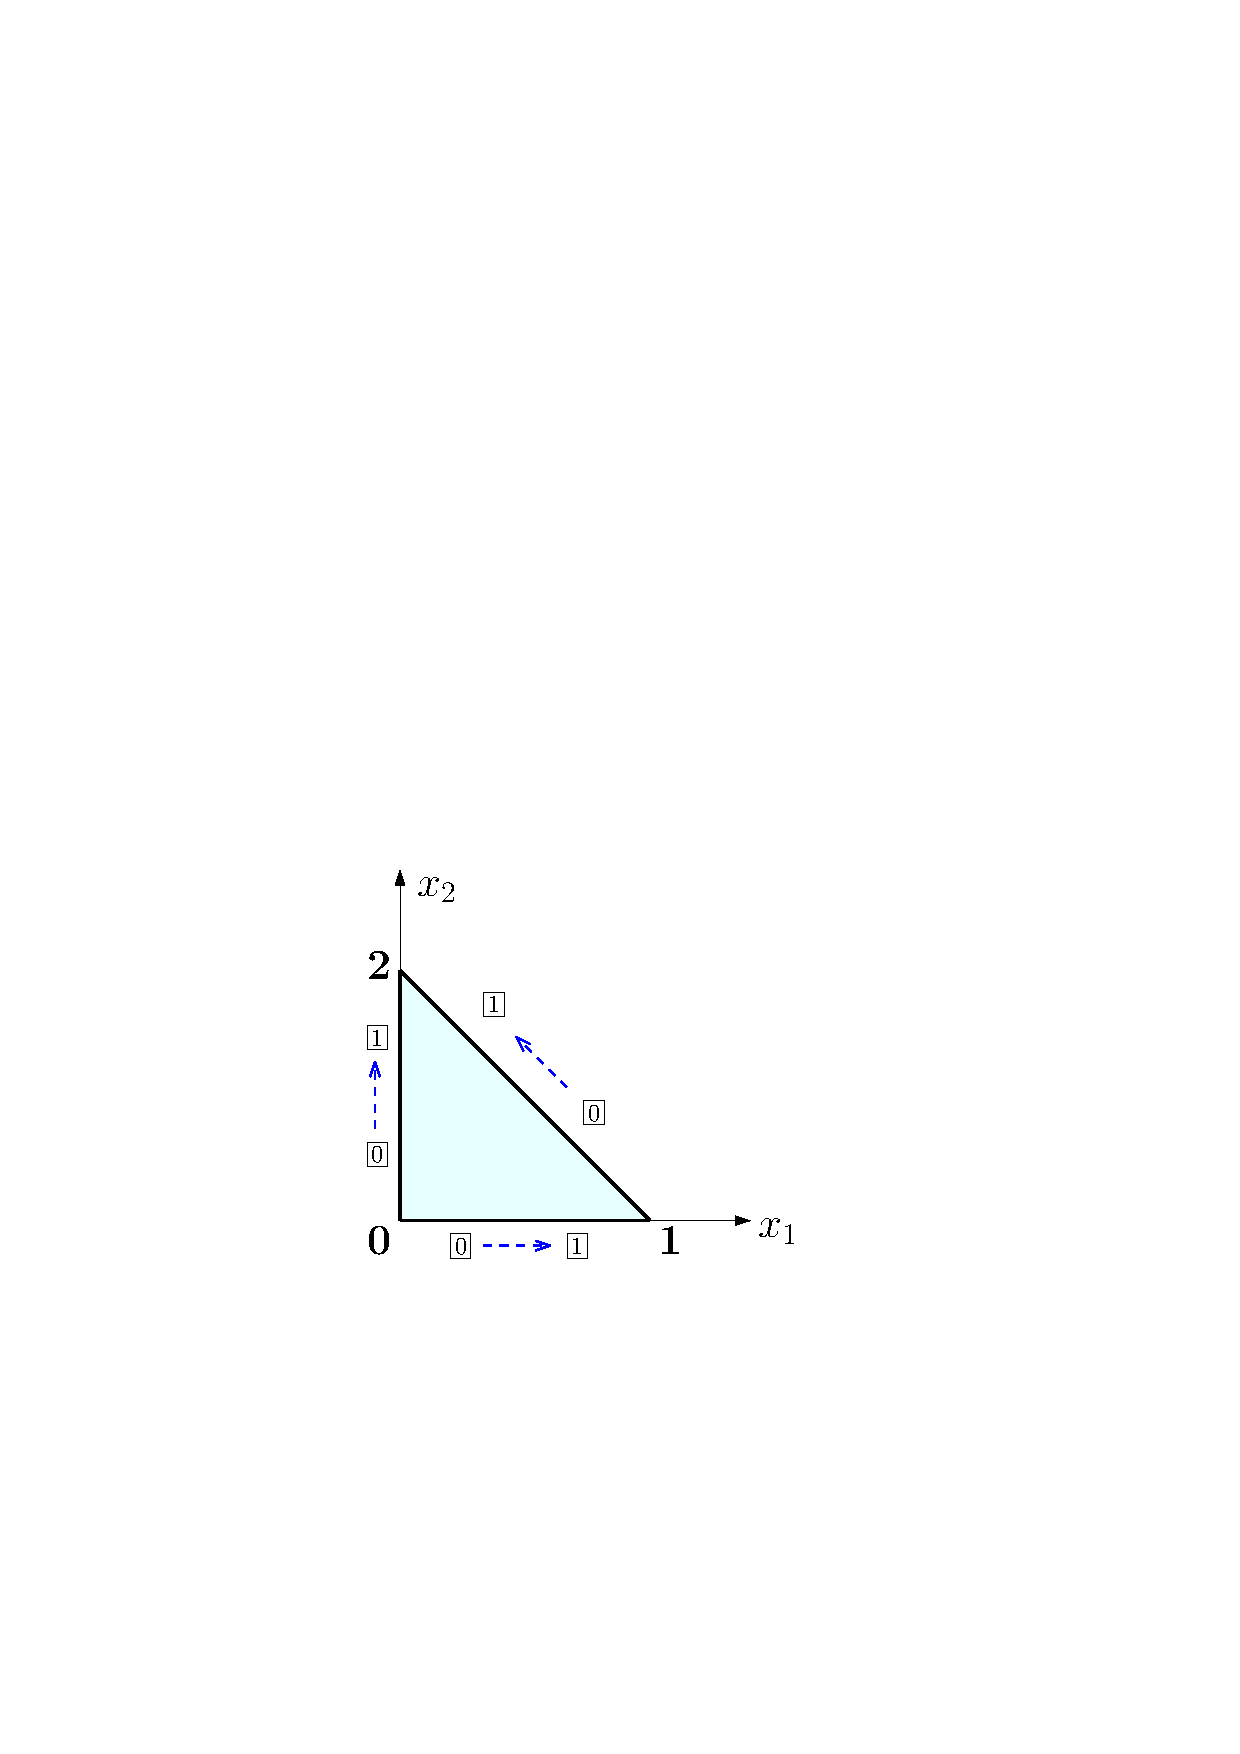
\includegraphics[scale=0.5]{./figures/MasterTriOrientations.pdf}
\caption{Master triangle with local edge orientations.}
\label{fig:MasterTriOrientations}
\end{center}
\end{figure}

The master triangle has a predefined \textit{local} orientation for each edge, which reperesents the $\oo=0$ case. 
These are shown in Figure \ref{fig:MasterTriOrientations}.
They are \textit{our} choices for the local orientations.

As with the quadrilateral, the local orientations induce a master element \textit{local} edge vertex-ordering which then determines a \textit{locally ordered} pair of affine coordinates. 
In the triangle, the correspondence between vertices and affine coordinates is trivial, since all one needs to know is that the vertex $v_a$ is linked to the affine coordinate $\nu_a$, where $a=0,1,2$.
As an example take the local edge orientations shown in Figure \ref{fig:MasterTriOrientations}.
Then, it is clear that the induced \textit{local} edge vertex-orderings are $v_0\tdashto v_1$, $v_1\tdashto v_2$ and $v_0\tdashto v_2$ for edges 01, 12 and 02 respectively.
Therefore, the \textit{locally ordered} pair of coordinates are $(\nu_0,\nu_1)$, $(\nu_1,\nu_2)$ and $(\nu_0,\nu_2)$.
These are then transformed to a \textit{globally ordered} pair via the edge local-to-global transformation $\sigma_\oo^\E$, and inputted into the different ancillary functions to give the orientation embedded shape functions.
For example, for edge 01, the orientation embedded $H^1$ edge functions are
\begin{equation*}
    \phi_i^\mathrm{e}(x)=\phi_i^\E\circ\sigma_\oo^\E(\vec{\nu}_{01}(x))
        =\begin{cases}
            \phi_i^\E\Big(\sigma_0^\E(\vec{\nu}_{01}(x))\Big)
            	=\phi_i^\E(\vec{\nu}_{01}(x))\,\,\,\text{if }\oo=0\,,\\
            \phi_i^\E\Big(\sigma_1^\E(\vec{\nu}_{01}(x))\Big)
            	=\phi_i^{\e}(\vec{\nu}_{10}(x))\,\,\,\text{if }\oo=1\,,
        \end{cases}
\end{equation*}
for $i=2,\ldots,p$.
For a more detailed example which analogously applies to the triangle see \S\ref{sec:QuadEdgeOrientations}.

\subsubsection{Triangle Face Orientations Explained}
\label{sec:TriaFaceOrientations}

%With triangles (as with quadrilaterals) it is not important to consider face orientations, since the boundary, which is shared with adjacent elements, is one dimensional.
%This means only edge orientations need to be considered.
%However, in three dimensions, the boundary is two dimensional and triangle faces will be shared by adjacent elements.
%It is required to match the corresponding shape functions over these faces to satisfy the compatibility condition.

In 3D, each face at the mesh must be given its own \textit{global face orientation} to ensure full compatibility across the boundaries.
For triangles, this is represented by the global triangle face coordinates $\Xi^\Tri=(\Xi_1^\Tri,\Xi_2^\Tri)$, or equivalently, by the \textit{global face vertex-ordering}.
For instance, given a triangle face in the mesh, a vertex-ordering of the form $a\tto b\tto c$ means the origin of $\Xi^\Tri$ is located at $a$, $\Xi_1^\Tri$ points from $a$ to $b$, and $\Xi_2^\Tri$ points from $a$ to $c$.
Meanwhile, at the master element, the mapped face has its own fixed \textit{local orientation}.
It is represented by the coordinates $\xi^\Tri=(\xi_1^\Tri,\xi_2^\Tri)$ or equivalently by the fixed \textit{local} ordering of the form $\boxednum{0}\!\tdashto\boxednum{1}\!\tdashto\boxednum{2}$.
In general, the two systems of coordinates will not match, and this mismatch is represented by the orientation parameter $\oo$.
For triangle faces, there are \textit{six} possible orientations, meaning $\oo=0,\ldots,5$.
These are all illustrated in Figure \ref{fig:OrientationsTri}.

\begin{figure}[!ht]
\begin{center}
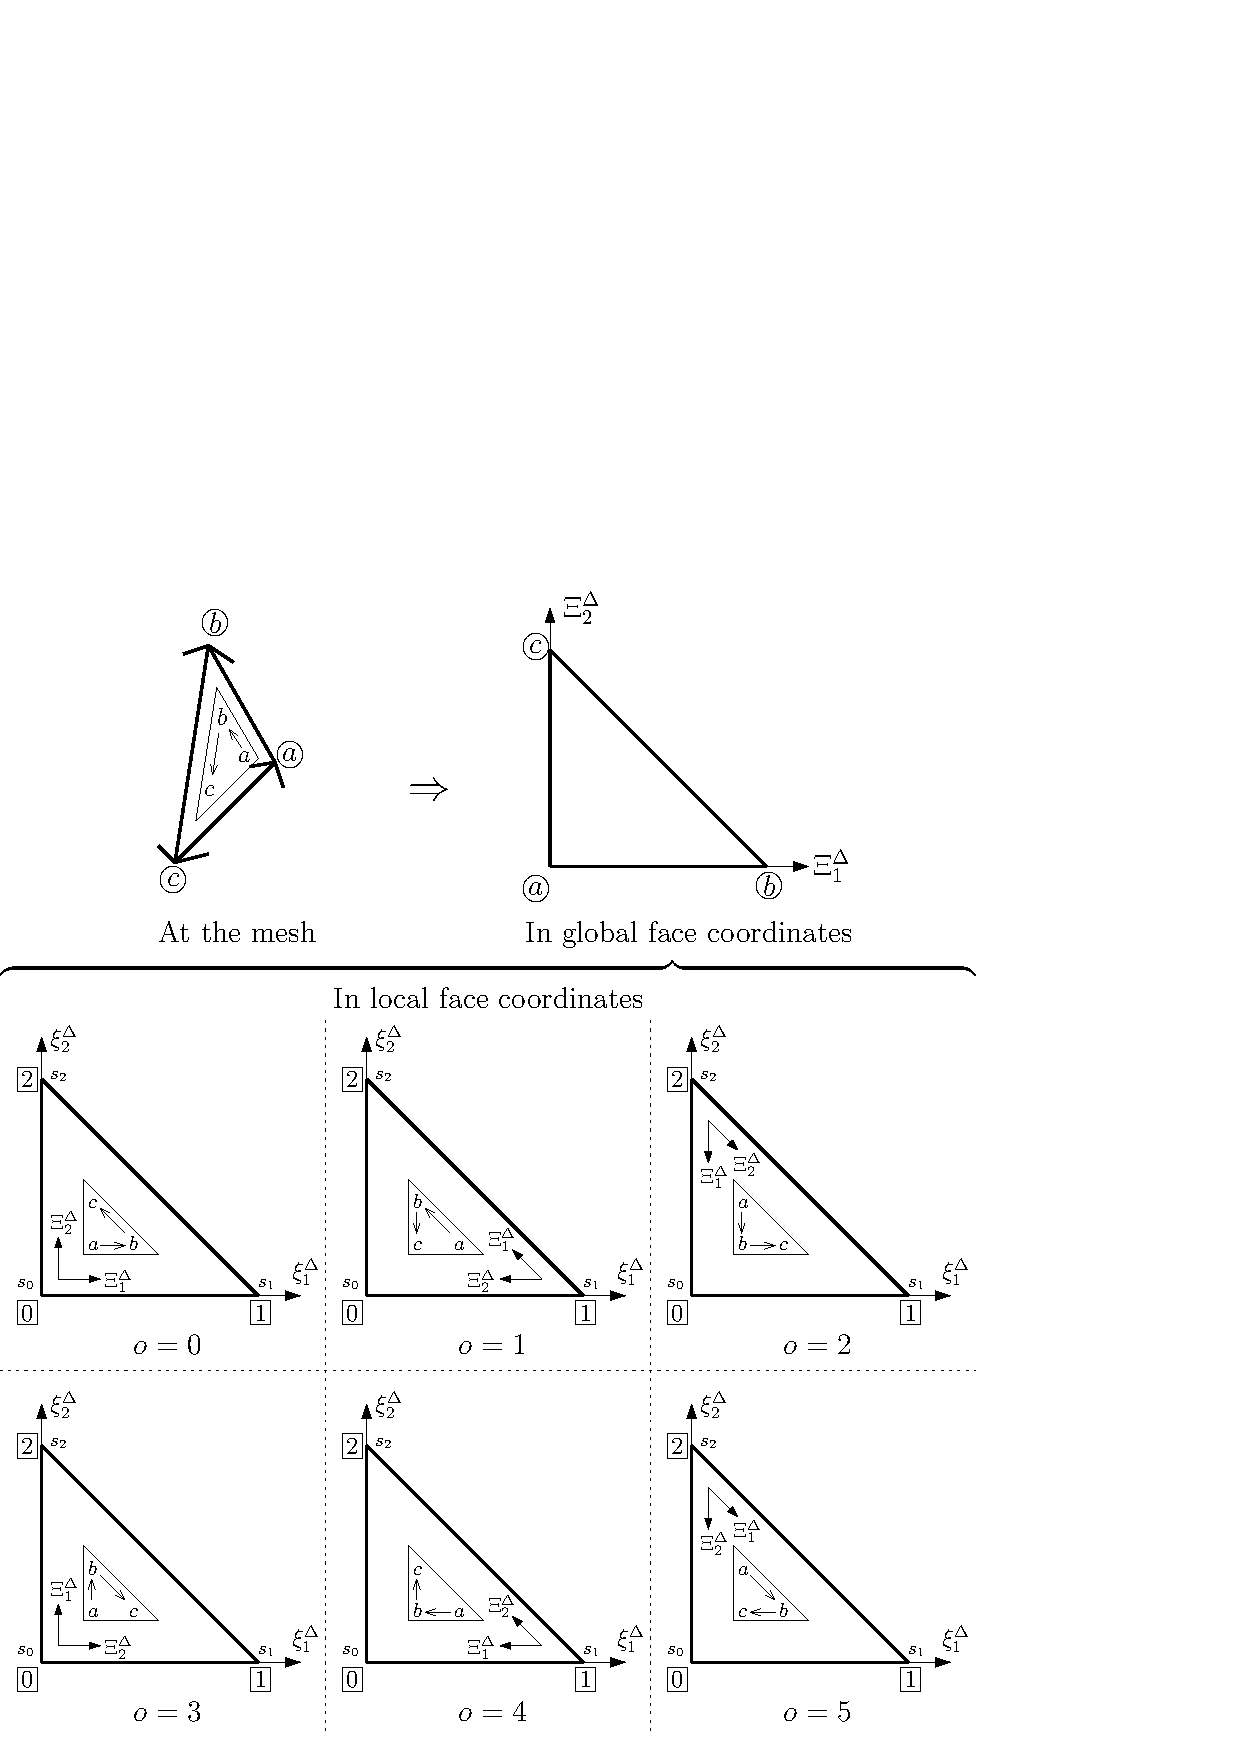
\includegraphics[scale=0.75]{./figures/OrientationsTriangle.pdf}
\caption{Triangle face orientations.}
\label{fig:OrientationsTri}
\end{center}
\end{figure}

Like quadrilaterals and edges, one needs a local-to-global transformation dependent on $\oo$.
For this, the \textit{local} orientation is represented by the \textit{locally ordered} triplet $(s_0,s_1,s_2)$.
The \textit{global} orientation is analogously represented by a \textit{globally ordered} triplet naturally induced from the \textit{global face vertex-ordering}.
For example, looking at Figure \ref{fig:OrientationsTri}, when $\oo=1$, the global ordering $a\tto b\tto c$ corresponds to the ordering $\boxednum{1}\!\tto\boxednum{2}\!\tto\boxednum{0}$, which in turn coresponds to the globally ordered triplet $(s_1,s_2,s_0)$.
Hence, once again the local-to-global transformation can be represented by a permutation, $\sigma_\oo^\Tri$, dependent on $\oo$.
It can be determined by observing Figure \ref{fig:OrientationsTri}.
Subsequently, all that is required is to compose the \textit{triangle face} ancillary functions and their differential form (those with superscript $\Tri$) with the local-to-global transformation $\sigma_\oo^\Tri$.
This should be done in all 3D shape functions associated to triangle faces.
More concrete examples will be given later.
Finally, the permutation function, $\sigma_\oo^\Tri$, is precisely defined next.

\begin{definition*}
Let $s_0$, $s_1$ and $s_2$ be arbitrary variables, and let $\oo=0,1,2,3,4,5$ be the triangle face orientation parameter. 
The triangle face orientation permutation function, $\sigma_\oo^\Tri$, is defined as
\begin{equation}
	\sigma_\oo^\Tri(s_0,s_1,s_2)=\begin{cases}
		\sigma_0^\Tri(s_0,s_1,s_2)=(s_0,s_1,s_2)&\quad\text{if  }\,\oo=0\,,\\
		\sigma_1^\Tri(s_0,s_1,s_2)=(s_1,s_2,s_0)&\quad\text{if  }\,\oo=1\,,\\
		\sigma_2^\Tri(s_0,s_1,s_2)=(s_2,s_0,s_1)&\quad\text{if  }\,\oo=2\,,\\
		\sigma_3^\Tri(s_0,s_1,s_2)=(s_0,s_2,s_1)&\quad\text{if  }\,\oo=3\,,\\
		\sigma_4^\Tri(s_0,s_1,s_2)=(s_1,s_0,s_2)&\quad\text{if  }\,\oo=4\,,\\
		\sigma_5^\Tri(s_0,s_1,s_2)=(s_2,s_1,s_0)&\quad\text{if  }\,\oo=5\,.\end{cases}\label{eq:orientTriFace}
\end{equation}
\end{definition*}

%In the case of triangles, everything can be understood by the way the three triangle vertices are listed. 
%For every face there is a predefined local numbering of the vertices, symbolized by $\xi^\mathrm{f}$ while there is a global numbering of the vertices, symbolized by $\Xi^\mathrm{f}$. There are \textit{six} different ways in which the vertices can be numbered. 
%That is, \textit{six} different possible global orientations represented by the parameter $\oo=0,\ldots,5$. They are shown in Figure \textit{add Figure}.
%
%Fortunately, these orientations are handled simply by permuting the entries of the triangular face functions: $\phi_{ij}^\Tri$, $E_{ij}^{\Delta_I}$, $E_{ij}^{\Delta_{II}}$, and in the future $V_{ij}^\Tri$.
%However, it should be mentioned that nontrivial pullback transforms are ocurring internally (but automatically) in the functions when the entries are permuted.
%
%To explain these permutations, the function $\vec{\sigma}$ is introduced as
%\begin{equation}
%    \begin{alignedat}{2}
%        \vec{\sigma}:\{0,1,2,3,4,5\}&\,\longrightarrow\,\{0,1,2\}\times\{0,1,2\}\times\{0,1,2\}\\
%        \oo\,&\,\longmapsto\,(\sigma_1(\oo),\sigma_2(\oo),\sigma_3(\oo))\,.
%    \end{alignedat}
%\end{equation}
%The function is more explicitly specified in Table \ref{table:functionSigma}.
%
%\begin{table}[ht]
%\begin{center}
%\begin{tabular}
%{|c|c|c|c|}\hline
%$\oo$ &$\sigma_1(\oo)$ & $\sigma_2(\oo)$  &  $\sigma_3(\oo)$ \\\hline\hline
%0 &0 & 1  & 2 \\\hline
%1 &2 & 0  & 1 \\\hline
%2 &1 & 2  & 0 \\\hline
%3 &0 & 2  & 1 \\\hline
%4 &1 & 0  & 2 \\\hline
%5 &2 & 1  & 0 \\\hline\hline
%\end{tabular}
%\caption{Function $\vec{\sigma}$.
%\label{table:functionSigma}}
%\end{center}
%\end{table}

%Now, $\phi_{ij}^\Tri$, $E_{ij}^{\Delta_I}$, $E_{ij}^{\Delta_{II}}$, and $V_{ij}^\Tri$ can simply be replaced with the new families of functions $\phi_{ij}^{\Delta,\oo}$, $E_{ij}^{\Delta_I,\oo}$, $E_{ij}^{\Delta_{II},\oo}$ and $V_{ij}^{\Delta,\oo}$ and their respective differentiated versions. Take for example $E_{ij}^{\Delta_{II},\oo}$, which becomes
%\begin{equation}
%    E_{ij}^{\Delta_{II},\oo}(s_0,s_1,s_2)=
%        E_{ij}^{\Delta_{II}}(s_{\sigma_1(\oo)},s_{\sigma_2(\oo)},s_{\sigma_3(\oo)})\,,
%\end{equation}
%for $i\geq0$, $j\geq1$ and $n=i+j=1,\ldots,p-1$. More explicitly,
%\begin{equation}
%    E_{ij}^{\Delta_{II},\oo}(s_0,s_1,s_2)=\begin{cases}
%    E_{ij}^{\Delta_{II},0}(s_0,s_1,s_2)=E_{ij}^{\Delta_{II}}(s_0,s_1,s_2)&\quad\text{if  }\,\oo=0\\
%    E_{ij}^{\Delta_{II},1}(s_0,s_1,s_2)=E_{ij}^{\Delta_{II}}(s_2,s_0,s_1)&\quad\text{if  }\,\oo=1\\
%    E_{ij}^{\Delta_{II},2}(s_0,s_1,s_2)=E_{ij}^{\Delta_{II}}(s_1,s_2,s_0)&\quad\text{if  }\,\oo=2\\
%    E_{ij}^{\Delta_{II},3}(s_0,s_1,s_2)=E_{ij}^{\Delta_{II}}(s_0,s_2,s_1)&\quad\text{if  }\,\oo=3\\
%    E_{ij}^{\Delta_{II},4}(s_0,s_1,s_2)=E_{ij}^{\Delta_{II}}(s_1,s_0,s_2)&\quad\text{if  }\,\oo=4\\
%    E_{ij}^{\Delta_{II},5}(s_0,s_1,s_2)=E_{ij}^{\Delta_{II}}(s_2,s_1,s_0)&\quad\text{if  }\,\oo=5\,,
%    \end{cases}
%\end{equation}
%for $i\geq0$, $j\geq1$ and $n=i+j=1,\ldots,p-1$.

%In view of future developments in the 3D element, we observe that triangular faces of {\em 3D} elements (such as the triangular faces of a tetrahedron, prism or pyramid) also has orientation in its own right, i.e., we need to consider the orientations of the face as well (as opposed to a simple 2D triangle with only one ``face'').
%To account for orientation embeddings in this case, we observe the following $6$ different orientations available to each triangle face of a 3D element.
%
%\begin{figure}[ht!]
%\centering
%\includegraphics[width=.9\textwidth]{./figures/triangle_orientations.png}
%        \caption{6 embedded orientations of the triangle face.}
%        \label{fig:TriangleOrientations}
%\end{figure}
%
%The orientations in the above figure induce $6$ permutations, $\sigma_\oo$ described in the following table.
%\begin{table}[ht]
%\begin{center}
%\begin{tabular}
%{|c|c|c|c|}\hline
%\oo &$\sigma_\oo(1)$ & $\sigma_\oo(2)$  &  $\sigma_\oo(3)$ \\\hline\hline
%0 &0 & 1  & 2 \\\hline
%1 &1 & 2  & 0 \\\hline
%2 &2 & 0  & 1 \\\hline
%3 &1 & 0  & 2 \\\hline
%4 &0 & 2  & 1 \\\hline
%5 &2 & 1  & 0 \\\hline\hline
%\end{tabular}
%\caption{Functions $\sigma_\oo$
%\label{table:functionSigma}}
%\end{center}
%\end{table}

%With the permutation functions $\sigma_\oo$, $\oo=0,\ldots,5$ given in Figure~\ref{table:functionSigma}, we can fully define the affine $H^1$ face shape function for the triangle faces of an arbitrary element with the affine coordinates $s_0,s_1,s_2$.
%\be
%\phi^{\Delta,\oo}_{ij}(s_0,s_1,s_2) = \left[L_i,L^{2i-1}_{j}\right] (s_{\sigma_\oo(0)},s_{\sigma_\oo(1)},s_{\sigma_\oo(2)})\,,
%\ee
%where $\oo=0,\ldots5$ denotes the given orientation of the affine coordinate system. The affine $H^1$ face shape function for all other faces are similarly defined. Here, the indices range $i\ge2,\, j\ge1,\, i+j \leq p$. 
%Section 6
\newpage
\section{Hexahedron}
\label{sec:Hexa}

\begin{figure}[!ht]
\begin{center}
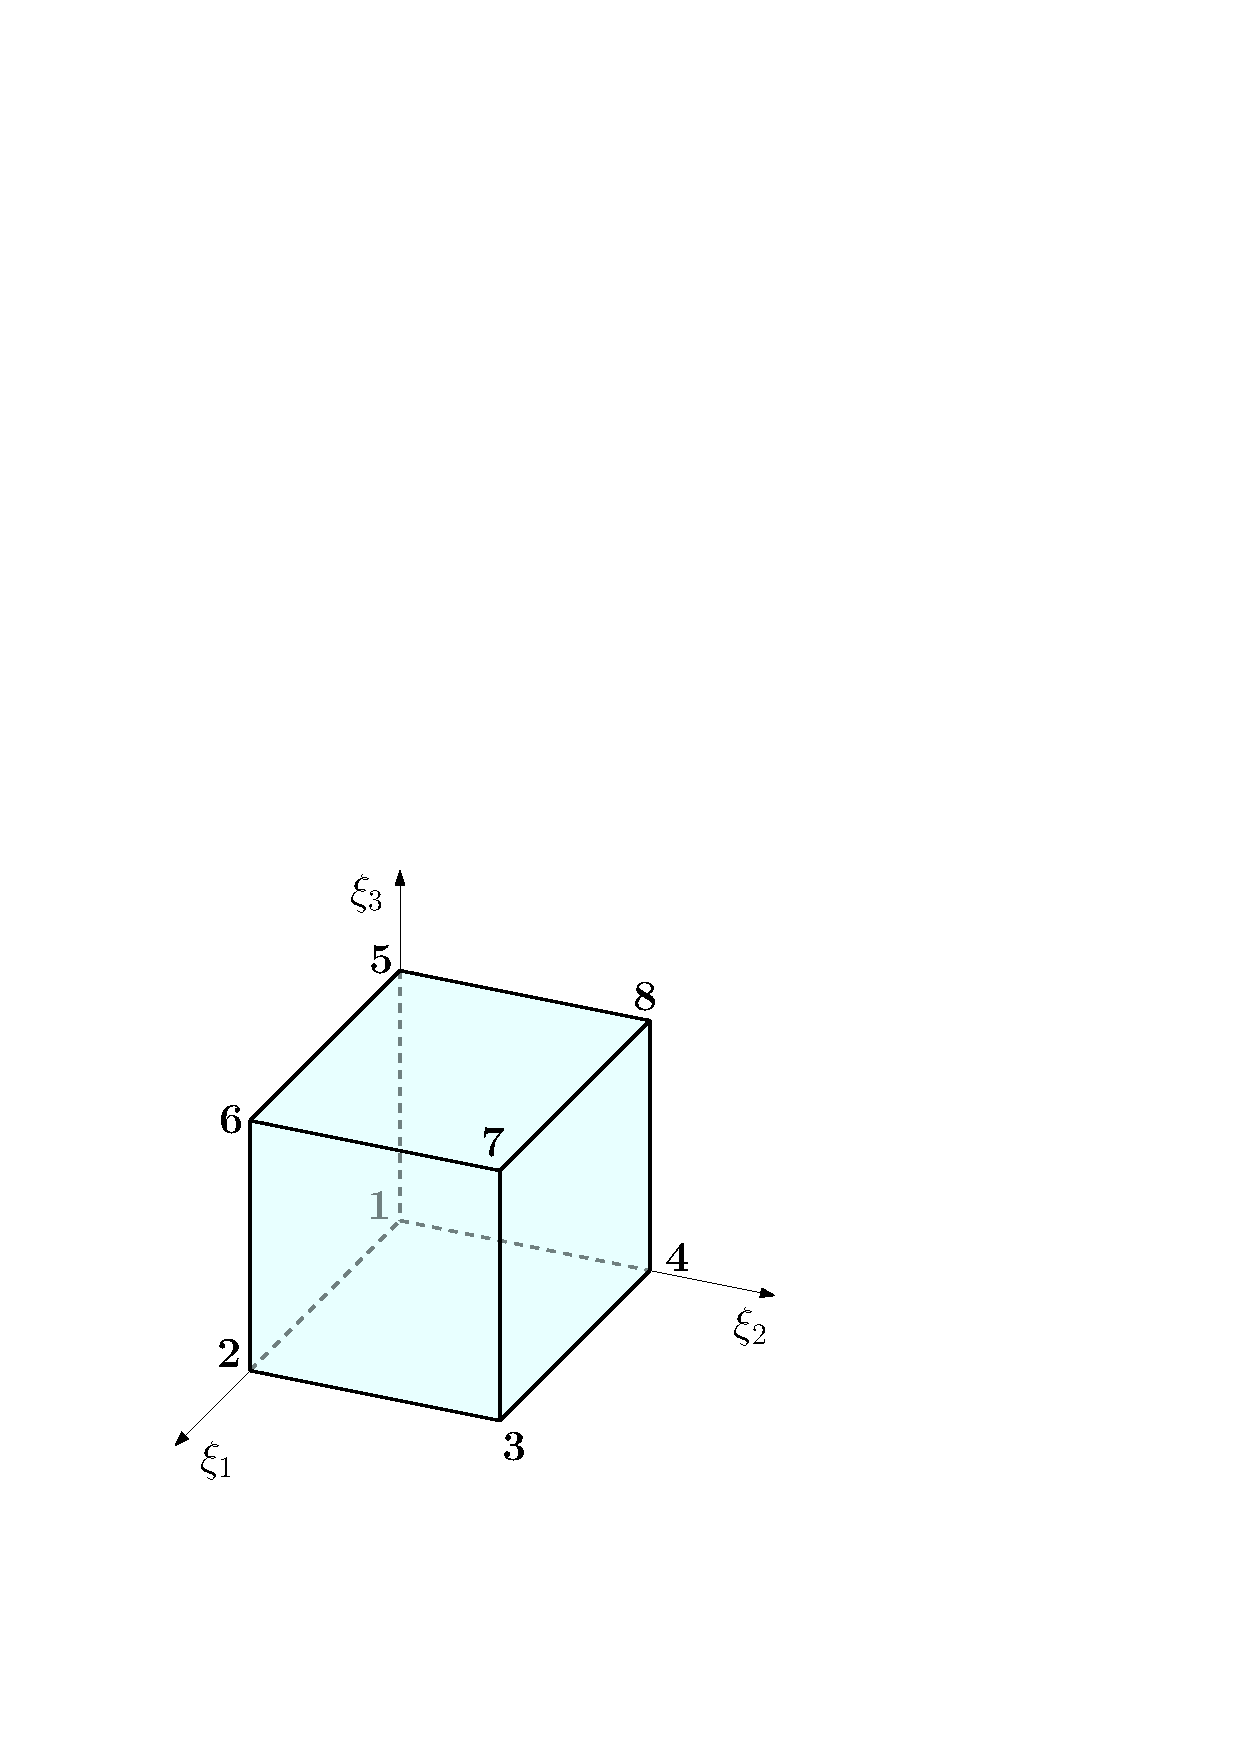
\includegraphics[scale=0.5]{./figures/MasterHexa.pdf}
\caption{Master hexahedron with numbered vertices.}
\label{fig:MasterHexa}
\end{center}
\end{figure}

The master element for hexahedra is $(0,1)^3$. 
It is shown in Figure \ref{fig:MasterHexa} in the $\xi=(\xi_1,\xi_2,\xi_3)$ space.
The master hexahedron is the Cartesian product of three segments.

%The master element for quadrilaterals is shown in Fig.~(\textit{add Figure}) in $\xi=(\xi_1,\xi_2,\xi_3)$ space.

There are \textit{three} pairs of 1D affine coordinates:
\begin{equation}
	\begin{alignedat}{4}
		\mu_0(\xi_1)&=1-\xi_1\,,\quad \mu_1(\xi_1)=\xi_1\,\qquad&\Rightarrow\qquad
			\nabla\mu_0(\xi_1)&=\bigg(\begin{smallmatrix}-1\\[2pt]0\\[2pt]0\end{smallmatrix}\bigg)\,,\quad
				\nabla\mu_1(\xi_1)=\bigg(\begin{smallmatrix}1\\[2pt]0\\[2pt]0\end{smallmatrix}\bigg)\,,\\
		\mu_0(\xi_2)&=1-\xi_2\,,\quad \mu_1(\xi_2)=\xi_2\,\qquad&\Rightarrow\qquad
			\nabla\mu_0(\xi_2)&=\bigg(\begin{smallmatrix}0\\[2pt]-1\\[2pt]0\end{smallmatrix}\bigg)\,,\quad
				\nabla\mu_1(\xi_2)=\bigg(\begin{smallmatrix}0\\[2pt]1\\[2pt]0\end{smallmatrix}\bigg)\,,\\
		\mu_0(\xi_3)&=1-\xi_3\,,\quad \mu_1(\xi_3)=\xi_3\,\qquad&\Rightarrow\qquad
			\nabla\mu_0(\xi_3)&=\bigg(\begin{smallmatrix}0\\[2pt]0\\[2pt]-1\end{smallmatrix}\bigg)\,,\quad
		\nabla\mu_1(\xi_3)=\bigg(\begin{smallmatrix}0\\[2pt]0\\[2pt]1\end{smallmatrix}\bigg)\,.
	\end{alignedat}
\end{equation}
These will be used explicitly or implicitly in the formulas that follow.

Just as with quadrilaterals, there are natural relationships between vertices, edges and faces, and the affine coordinates.
In fact, each vertex is linked to \textit{three} affine coordinates, each edge is linked to \textit{two} affine coordinates, and each face is linked to \textit{one} affine coordinate.
The linked affine coordinates take the value $1$ at the associated topological entity.
For example, vertex $1$, $v_1=(0,0,0)$, is linked to the affine coordinates $\mu_0(\xi_1)$, $\mu_0(\xi_2)$ and $\mu_0(\xi_3)$, edge 12 is linked to the affine coordinates $\mu_0(\xi_2)$ and $\mu_0(\xi_3)$, and face 1234 is linked to affine coordinate $\mu_0(\xi_3)$.

\subsubsection*{Exact Sequence}
%The three dimensional exact sequence is of the form 
%\begin{equation}
%H^1 \xrightarrow{\,\,\nabla\,\,} H(\mathrm{curl}) \xrightarrow{\nabla\times} H(\mathrm{div}) \xrightarrow{\nabla\cdot} L^2 \,.
%\label{eq:3DExactSeq}
%\end{equation}

Recall the 3D exact sequence for simply connected domains \eqref{eq:3D_exact_sequence}.
The corresponding discrete polynomial exact sequence is of the form 
\begin{equation}
	W^{p,q,r} \xrightarrow{\,\,\nabla\,\,} Q^{p,q,r} \xrightarrow{\nabla\times} V^{p,q,r} \xrightarrow{\nabla\cdot} Y^{p,q,r} \,,
\end{equation}
where the standard N\'{e}d\'{e}lec's spaces \cite{Nedelec80} of the first type for the hexahedron are utilized:
\begin{equation}
	\begin{aligned}
	W^{p,q,r} & = \mathcal{Q}^{p,q,r}= \mathcal{P}^p(\xi_1)\otimes \mathcal{P}^q (\xi_2)\otimes \mathcal{P}^r (\xi_3)\,,\\
	Q^{p,q,r} & = \mathcal{Q}^{p-1,q,r} \times\mathcal{Q}^{p,q-1,r}\times \mathcal{Q}^{p,q,r-1}\,,\\
	V^{p,q,r} & = \mathcal{Q}^{p,q-1,r-1} \times\mathcal{Q}^{p-1,q,r-1}\times \mathcal{Q}^{p-1,q-1,r}\,,\\
	Y^{p,q,r} & = \mathcal{Q}^{p-1,q-1,r-1}\,.
	\end{aligned}
\end{equation}
%Again, we follow the construction of Ainsworth and Coyle\cite{AinsworthCoyle01} based on mimicking the structure of \Nedelec's spaces with Legendre and Lobatto (integrated Legendre) polynomials. The ideas are simply extrapolated from the quadrilateral case.
As with the quadrilateral, there is a natural anisotropy of the element, which has order $p$ in the $\xi_1$ direction, $q$ in the $\xi_2$ direction and $r$ in the $\xi_3$ direction. 
The hierarchy should be maintained in $p$, $q$ and $r$ separately.  
It will sometimes be convenient to refer to $p_a$ as the order in the $\xi_a$ direction, so that $p_1=p$, $p_2=q$ and $p_3=r$.


\subsection{\texorpdfstring{$H^1$}{H1} Shape Functions}
%Recall that in three dimensions, the trace of $H^1$ functions is the value of the function itself along the boundary. 
%Hence, vertex functions should vanish at all nonadjacent faces, edge functions should vanish at all nonadjacent faces, face functions should vanish at all other faces, and bubbles should vanish at all faces. 
It will be clear that the $(p+1)(q+1)(r+1)$ shape functions defined in this section lie in $\mathcal{Q}^{p,q,r}$ and span the space.

The ideas in this section are the same as with the quadrilateral (see \S\ref{sec:Quad}) but in three dimensions.
This will simply translate to adding an extra blending function to account for the extra dimension.
Hence, the trace properties will not be analyzed in detail as they easily follow.

\subsubsection{\texorpdfstring{$H^1$}{H1} Vertices}
%First note there are three pairs of 1D affine coordinates:
%\begin{equation}
%	\begin{alignedat}{4}
%		\mu_0(\xi_1)&=1-\xi_1\,,\quad \mu_1(\xi_1)=\xi_1\,,\qquad&\Rightarrow\qquad
%			\nabla\mu_0(\xi_1)&=\bigg(\begin{smallmatrix}-1\\0\\0\end{smallmatrix}\bigg)\,,\quad
%				\nabla\mu_1(\xi_1)=\bigg(\begin{smallmatrix}1\\0\\0\end{smallmatrix}\bigg)\\
%		\mu_0(\xi_2)&=1-\xi_2\,,\quad \mu_1(\xi_2)=\xi_2\,,\qquad&\Rightarrow\qquad
%			\nabla\mu_0(\xi_2)&=\bigg(\begin{smallmatrix}0\\-1\\0\end{smallmatrix}\bigg)\,,\quad
%				\nabla\mu_1(\xi_2)=\bigg(\begin{smallmatrix}0\\1\\0\end{smallmatrix}\bigg)\\
%		\mu_0(\xi_3)&=1-\xi_3\,,\quad \mu_1(\xi_3)=\xi_3\,,\qquad&\Rightarrow\qquad
%			\nabla\mu_0(\xi_3)&=\bigg(\begin{smallmatrix}0\\0\\-1\end{smallmatrix}\bigg)\,,\quad
%		\nabla\mu_1(\xi_2)=\bigg(\begin{smallmatrix}0\\0\\1\end{smallmatrix}\bigg)\,.
%	\end{alignedat}
%\end{equation}
%These will be used explicitly or implicitly in the formulas that follow.
%The vertex functions will be products of these:
Without any delays, the vertex shape functions and their gradient are
\begin{equation}
	\begin{aligned}
		\phi^\mathrm{v}(\xi)&=\mu_a(\xi_1)\mu_b(\xi_2)\mu_c(\xi_3)\,,\\
		\nabla\phi^\mathrm{v}(\xi)&=\mu_a(\xi_1)\mu_b(\xi_2)\nabla\mu_c(\xi_3)+\mu_c(\xi_3)\mu_a(\xi_1)\nabla\mu_b(\xi_2)
			+\mu_b(\xi_2)\mu_c(\xi_3)\nabla\mu_a(\xi_1)\,,
	\end{aligned}
\end{equation}
for $a=0,1$, $b=0,1$ and $c=0,1$. 
There are a total of $8$ vertex functions (one for each vertex).

%Their gradients are
%\begin{equation}
%	\nabla\phi^\mathrm{v}(\xi)=\mu_a(\xi_1)\mu_b(\xi_2)\nabla\mu_c(\xi_3)+\mu_c(\xi_3)\mu_a(\xi_1)\nabla\mu_b(\xi_2)
%		+\mu_b(\xi_2)\mu_c(\xi_3)\nabla\mu_a(\xi_1)\,.
%\end{equation} 
%As required they vanish at all vertices except the one with coordinates $(a,b,c)$. 
%By linearity this means they also vanish at all nonadjacent edges and faces.
%Moreover, their traces over adjacent edges are of the form $\mu_b(\xi_a)$ for some $a=1,2,3$ and $b=0,1$, which coincides with the segment case. 
%The same applies to the traces over adjacent faces, which coincide with the quadrilateral face. 
%This makes the traces compatible with any potential neighboring element.
%
%Throughout the rest of this section $\vec{\mu}_{01}(\xi_a)=(\mu_0(\xi_a),\mu_1(\xi_a))$ for $a=1,2,3$, while $p_a$ is the order in the $\xi_a$ axis. That is $p_1=p$, $p_2=q$ and $p_3=r$.

\subsubsection{\texorpdfstring{$H^1$}{H1} Edges}

Again, this is analogous to the quadrilateral case, but with an extra blending function. 
Take for example edge 12.
Then, the shape functions are
\begin{equation*}
	\phi_i^\mathrm{e}(\xi)=\underbrace{\mu_0(\xi_3)\mu_0(\xi_2)}_{\text{blend}}
		 \underbrace{\phi_i^\E(\underbrace{\vec{\mu}_{01}(\xi_1)}_{\text{project}})}_{\text{evaluate}}\,,
\end{equation*}
for $i=2,\ldots,p$. 
The projection being implied is:
\begin{equation*}
	(\xi_1,\xi_2,\xi_3)\;\longmapsto\;(\xi_1,\xi_2,0)\;\longmapsto\;(\xi_1,0,0)\,.
\end{equation*}
It is illustrated in Figure \ref{fig:HexaProjection}. 
It consists simply of finding the intersection $P''=(\xi_1,0,0)$ of the edge with the normal plane passing through the original point $P=(\xi_1,\xi_2,\xi_3)$.
Alternatively it can be interpreted in two steps.
First it is projected to the closest point $P'$ in an adjacent face, by using the normal to the face.
Once in the face, it is projected again to the desired edge using the traditional \textit{two} dimensional quadrilateral projection (see Figure \ref{fig:QuadProjection}).
%by using the normal to that face and then it is projected to the desired edge by using the normal

\begin{figure}[!ht]
\begin{center}
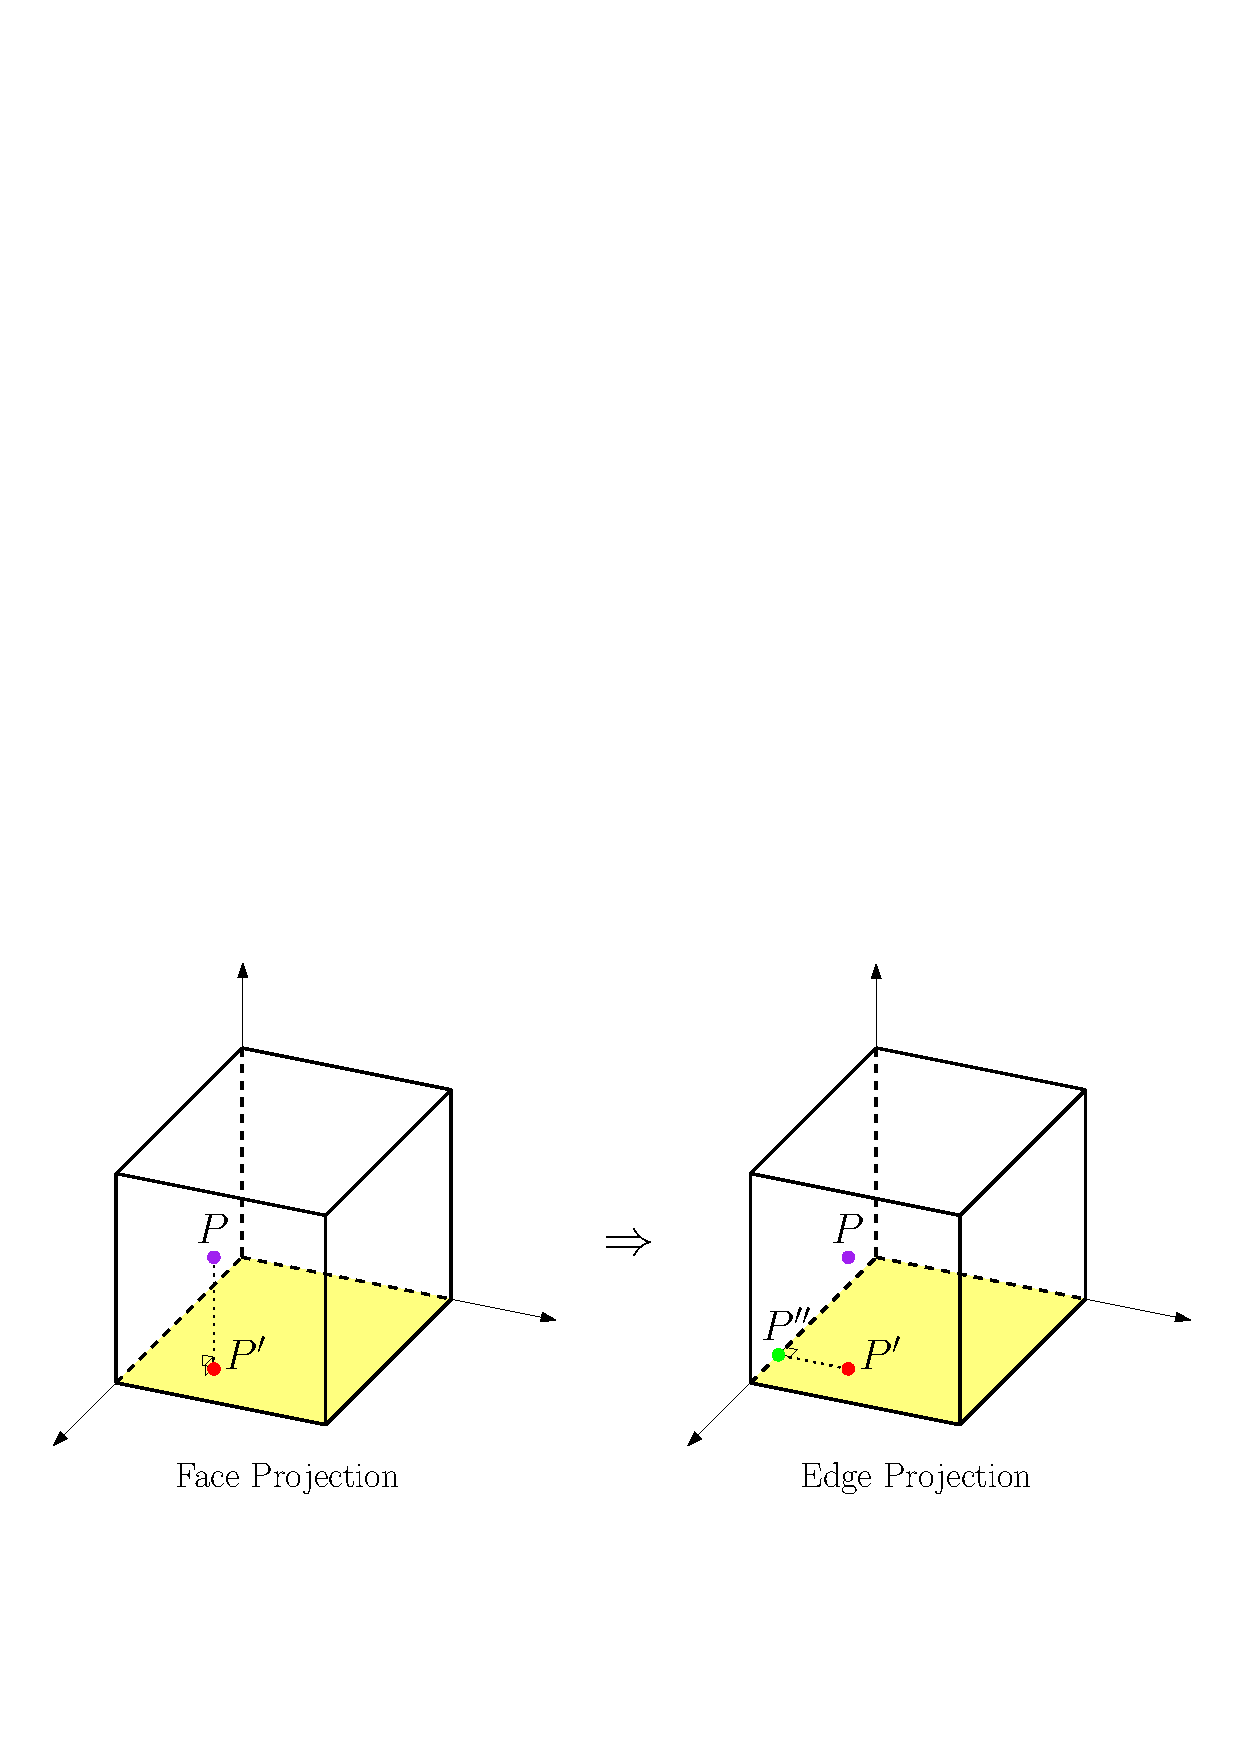
\includegraphics[scale=0.6]{./figures/HexaProjection.pdf}
\caption{Face projection from $P$ to $P'$ followed by an edge projection from $P'$ to $P''$.}
\label{fig:HexaProjection}
\end{center}
\end{figure}

%One can readily check that the required vanishing conditions and trace properties are satisfied over edges and faces.

%Again, there is an edge projection (in three dimenions) being implied:
%\begin{equation*}
%	(\xi_1,\xi_2,\xi_3)\;\longmapsto\;(\xi_1,0,0)\,.
%\end{equation*}
%It consists simply of finding the intersection $P'=(\xi_1,0,0)$ of the edge with the normal plane passing through the original point $P=(\xi_1,\xi_2,\xi_3)$. 
%This is illustrated in Fig.~(\textit{add Figure}).

The general edge shape functions and their gradient are
\begin{equation}
	\begin{aligned}
		\phi_i^\mathrm{e}(\xi)&=\mu_e(\xi_c)\mu_d(\xi_b)\phi_i^\E(\vec{\mu}_{01}(\xi_a))\,,\\
		\nabla\phi_i^\mathrm{e}(\xi)&=\mu_e(\xi_c)\mu_d(\xi_b)\nabla\phi_i^\E(\vec{\mu}_{01}(\xi_a))
			+\phi_i^\E(\vec{\mu}_{01}(\xi_a))\Big(\mu_e(\xi_c)\nabla\mu_d(\xi_b)+\mu_d(\xi_b)\nabla\mu_e(\xi_c)\Big)\,,
	\end{aligned}
	\label{eq:Hexaphigeneral}
\end{equation}
where $i=2,\ldots,p_a$, $(a,b,c)=(1,2,3),(2,3,1),(3,1,2)$, $d=0,1$ and $e=0,1$.
%Their gradients are
%\begin{equation}
%	\begin{aligned}
%		\nabla\phi_i^\mathrm{e}(\xi)=\mu_e(\xi_c)\mu_d(\xi_b)\nabla\phi_i^\E(\vec{\mu}_{01}(\xi_a))
%			+\phi_i^\E(\vec{\mu}_{01}(\xi_a))\Big(\mu_e(\xi_c)\nabla\mu_d(\xi_b)+\mu_d(\xi_b)\nabla\mu_e(\xi_c)\Big)\,.
%		\end{aligned}
%\end{equation}
For example for edge 12, this would correspond to $(a,b,c)=(1,2,3)$, $d=0$, $e=0$ and $p_a=p$, for edge 23 it is $(a,b,c)=(2,3,1)$, $d=0$, $e=1$ and $p_a=q$, and so on. 
For each edge there are $p_a-1$ shape functions, leading to a total of $4(p-1)+4(q-1)+4(r-1)$ edge functions.

%\paragraph{Edge Orientations.} These are dealt with analogously to the quadrilateral edge orientations (see the note on edge orientations in \S\ref{sec:H1edgesQuad}).

\subsubsection{\texorpdfstring{$H^1$}{H1} Faces}

Again, by adding as a blending factor the associated affine coordinate the construction becomes trivial. 
For example, for face 1234, the shape functions are
\begin{equation*}
	\phi_{ij}^\mathrm{f}(\xi)=\underbrace{\mu_0(\xi_3)}_{\text{blend}}
		\underbrace{\phi_{ij}^\square(\underbrace{\vec{\mu}_{01}(\xi_1),\vec{\mu}_{01}(\xi_2)}_{\text{project}})}_{\text{evaluate}}\,,
\end{equation*}
where $i=2,\ldots,p$ and $j=2,\ldots,q$. 
The projection is already illustrated in Figure \ref{fig:HexaProjection}, and simply consists of finding the intersection $P'=(\xi_1,\xi_2,0)$ of the normal to the face that passes through the original point $P=(\xi_1,\xi_2,\xi_3)$.
%
%Now there is \textit{face} projection involved:
%\begin{equation*}
%	(\xi_1,\xi_2,\xi_3)\;\longmapsto\;(\xi_1,\xi_2,0)\,.
%\end{equation*}
%It consists of finding the intersection $P'=(\xi_1,\xi_2,0)$ of the face with the normal line passing through the original point $P=(\xi_1,\xi_2,\xi_3)$. 
%This is shown in Fig.~(\textit{add Figure}).

In general the face shape functions and their gradient are
\begin{equation}
	\begin{aligned}
		\phi_{ij}^\mathrm{f}(\xi)&=\mu_d(\xi_c)\phi_{ij}^\square(\vec{\mu}_{01}(\xi_a),\vec{\mu}_{01}(\xi_b))\,,\\
		\nabla\phi_{ij}^\mathrm{f}(\xi)&=\mu_d(\xi_c)\nabla\phi_{ij}^\square(\vec{\mu}_{01}(\xi_a),\vec{\mu}_{01}(\xi_b))
			+\phi_{ij}^\square(\vec{\mu}_{01}(\xi_a),\vec{\mu}_{01}(\xi_b))\nabla\mu_d(\xi_c)\,,
	\end{aligned}
	\label{eq:Hexaphifacegeneral}
\end{equation}
where $i=2,\ldots,p_a$, $j=2,\ldots,p_b$, $(a,b,c)=(1,2,3),(2,3,1),(3,1,2)$, and $d=0,1$.
%Their gradients are
%\begin{equation}
%	\nabla\phi_{ij}^\mathrm{f}(\xi)=\mu_d(\xi_c)\nabla\phi_{ij}^\square(\vec{\mu}_{01}(\xi_a),\vec{\mu}_{01}(\xi_b))
%		+\phi_{ij}^\square(\vec{\mu}_{01}(\xi_a),\vec{\mu}_{01}(\xi_b))\nabla\mu_d(\xi_c)\,.\label{gradfacephiHexa}
%\end{equation}
For example for face 1234, this would correspond to $(a,b,c)=(1,2,3)$, $d=0$, $p_a=p$ and $p_b=q$, for face 1265 it is $(a,b,c)=(3,1,2)$, $d=0$, $p_a=r$ and $p_b=p$, and so on. 
For each face there are $(p_a-1)(p_b-1)$ shape functions, for a total of $2(p-1)(q-1)+2(q-1)(r-1)+2(r-1)(p-1)$ face functions.
%Clearly, this construction ensures all the desired trace properties which are consistent with the quadrilateral and segment elements.

%Notice that in \eqref{eq:Hexaphifacegeneral} the functions $\phi_{ij}^\square$ and $\nabla\phi_{ij}^\square$ are explicitly used, instead of simply writing products of $\phi_i^\E$ or even more so $L_i$. 
%Writing $\phi_{ij}^\square$ is preferred, because it reflects that the formula is representative of a quadrilateral face. 
%More importantly, when orientations play a role, it is much more convenient to have the equations in this form, since the local-to-global transformation directly handles permutations of quadruples.

%how the shape functions should be coded, since $\phi_{ij}^\square$ is called in multiple occasions from the different elements (in more general settings). 
%More importantly, these simplifications should be avoided, since by the time orientations are handled, they will change depending on the orientation.
%But with $\phi_{ij}^\square$ written directly, when orientations are included, it is a simple matter of appropriately permuting the entries of $\phi_{ij}^\square$ and $\nabla\phi_{ij}^\square$ to get the right expressions. This is shown next with an example.

%\paragraph{Face Orientations.} To consider orientations, simply take a predefined $\oo=0$ orientation for a given quadrilateral face, and replace $\phi_{ij}^\square$ with $\phi_{ij}^{\square,\oo}$ (and similarly with the gradients). For example take face 1265. The first predefined local face axis for this face, $\xi_1^\mathrm{f}$, which determines the first two entries of $\phi_{ij}^{\square,\oo}$, is parallel with the master element axis $\xi_1$. The second predefined local face axis for this face, $\xi_2^\mathrm{f}$, which determines the second pair of entries in $\phi_{ij}^{\square,\oo}$, is parallel with the master element axis $\xi_3$. Now, $\xi_1^\mathrm{f}$ and $\xi_1$ point in the same direction, meaning the first two entries of $\phi_{ij}^{\square,\oo}$ are organized as $(\mu_0(\xi_1),\mu_1(\xi_1))$ (and \textit{not} $(\mu_1(\xi_1),\mu_0(\xi_1))$). The same applies to $\xi_2^\mathrm{f}$ and $\xi_3$, which also point in the same direction. This defines the $\oo=0$ orientation, so that \eqref{eq:Hexaphifacegeneral} becomes
%\begin{equation*}
%	\phi_{ij}^\mathrm{f}(\xi)=\mu_0(\xi_2)\phi_{ij}^{\square,\oo}(\mu_0(\xi_1),\mu_1(\xi_1),\mu_0(\xi_3),\mu_1(\xi_3))\,.
%\end{equation*}
%Then, depending on the orientation $\oo$ (that is, depending on the placement of the global axes $\Xi_1^\mathrm{f}$ and $\Xi_2^\mathrm{f}$), the function will take a different form. 
%It amounts to evaluating the original function $\phi_{ij}^{\square}$ but with the entries permuted in different ways. 
%To learn how to do these permutations depending on $\oo$ see \S\ref{sec:QuadFaceOrientations}. 
%As an example, assume $\oo=1$. In that case,
%\begin{equation*}
%	\phi_{ij}^\mathrm{f}(\xi)=\mu_0(\xi_2)\phi_{ij}^{\square,1}(\mu_0(\xi_1),\mu_1(\xi_1),\mu_0(\xi_3),\mu_1(\xi_3))
%		=\mu_0(\xi_2)\phi_{ij}^{\square}(\mu_1(\xi_3),\mu_0(\xi_3),\mu_0(\xi_1),\mu_1(\xi_1))\,.
%\end{equation*}
%for $i=2,\ldots,r$ and $j=2,\ldots,p$. The same applies for the gradients, and for future face functions that will follow (which will involve $E_{ij}^\square$, $E_{ij}^\square$ and $V_{ij}^\square$).

\subsubsection{\texorpdfstring{$H^1$}{H1} Interior Bubbles}

These are constructed like the face functions, but by using edge bubbles $\phi_k^\E$ instead of the linear blending factor $\mu_d$. 
This will ensure the necessary vanishing trace properties.

The interior bubbles and their gradient are
\begin{equation}
	\begin{aligned}
		\phi_{ijk}^\mathrm{b}(\xi)&=L_i(\mu_1(\xi_1))L_j(\mu_1(\xi_2))L_k(\mu_1(\xi_3))
			=\phi_{ij}^\square(\vec{\mu}_{01}(\xi_1),\vec{\mu}_{01}(\xi_2))\phi_k^\E(\vec{\mu}_{01}(\xi_3))\,,\\
		\nabla\phi_{ijk}^\mathrm{b}(\xi)&=
			\phi_{ij}^\square(\vec{\mu}_{01}(\xi_1),\vec{\mu}_{01}(\xi_2))\nabla\phi_k^\E(\vec{\mu}_{01}(\xi_3))
				+\phi_k^\E(\vec{\mu}_{01}(\xi_3))\nabla\phi_{ij}^\square(\vec{\mu}_{01}(\xi_1),\vec{\mu}_{01}(\xi_2))\,,
	\end{aligned}
\end{equation}
for $i=2,\ldots,p$, $j=2,\ldots,q$ and $k=2,\ldots,r$. 
%Their gradients are
%\begin{equation}
%\begin{aligned}
%	\nabla\phi_{ijk}^\mathrm{b}(\xi)&=\phi_{ij}^\square(\vec{\mu}_{01}(\xi_1),\vec{\mu}_{01}(\xi_2))\nabla\phi_k^\E(\vec{\mu}_{01}(\xi_3))
%		+\phi_k^\E(\vec{\mu}_{01}(\xi_3))\nabla\phi_{ij}^\square(\vec{\mu}_{01}(\xi_1),\vec{\mu}_{01}(\xi_2))\\
%	&=\begin{pmatrix}P_{i-1}(\xi_1)L_j(\xi_2)L_k(\xi_3)\\L_i(\xi_1)P_{j-1}(\xi_2)L_k(\xi_3)\\
%		L_i(\xi_1)L_j(\xi_2)P_{k-1}(\xi_3)
%		\end{pmatrix}\,.
%\end{aligned}
%\end{equation}
Clearly there will be $(p-1)(q-1)(r-1)$ interior bubbles.



\subsection{\texorpdfstring{$H(\mathrm{curl})$}{Hcurl} Shape Functions}

%The trace of $H(\mathrm{curl})$ functions is the value of the tangential component of the vector function along the boundary (the edges and faces).
%This means all edge functions should have vanishing trace at all nonadjacent faces, face functions should have zero trace at all other faces, and bubbles should have zero trace at all faces.
It will be clear that the $p(q+1)(r+1)+q(r+1)(p+1)+r(p+1)(q+1)$ linearly independent shape functions span $Q^{p,q,r}=\mathcal{Q}^{p-1,q,r}\times\mathcal{Q}^{p,q-1,r}\times\mathcal{Q}^{p,q,r-1}$ as required.

The ideas in this section are the same as with the quadrilateral but in three dimensions. 
This will simply translate to adding an extra blending function to account for the extra dimension.
The structure of projecting, evaluating and blending still holds in $H(\mathrm{curl})$, and the projections (and even the blending functions) are the same as those in $H^1$.
As with $H^1$, the analysis of the trace properties will be superfluous.

\subsubsection{\texorpdfstring{$H(\mathrm{curl})$}{Hcurl} Edges}
These will just be the quadrilateral edge functions with the extra blending factor. They are
\begin{equation}
	\begin{aligned}
		E_i^\mathrm{e}(\xi)&=\mu_e(\xi_c)\mu_d(\xi_b)E_i^\E(\vec{\mu}_{01}(\xi_a))\,,\\
		\nabla\times E_i^\mathrm{e}(\xi)&=
			\Big(\mu_e(\xi_c)\nabla\mu_d(\xi_b)+\mu_d(\xi_b)\nabla\mu_e(\xi_c)\Big)\times E_i^\E(\vec{\mu}_{01}(\xi_a))\,,
	\end{aligned}
\end{equation}
where $i=2,\ldots,p_a$, $(a,b,c)=(1,2,3),(2,3,1),(3,1,2)$, $d=0,1$ and $e=0,1$.
%Their curls are
%\begin{equation}
%	\begin{aligned}
%		\nabla\times E_i^\mathrm{e}(\xi)=
%			\Big(\mu_e(\xi_c)\nabla\mu_d(\xi_b)+\mu_d(\xi_b)\nabla\mu_e(\xi_c)\Big)\times E_i^\E(\vec{\mu}_{01}(\xi_a))\,.
%	\end{aligned}
%\end{equation}
Notice the form is very similar to that of edge $H^1$ functions. 
For each edge there are $p_a$ shape functions, giving a total of $4p+4q+4r$ edge functions. 


\subsubsection{\texorpdfstring{$H(\mathrm{curl})$}{Hcurl} Faces}

The pattern goes on, but this time with the two families.
There are a grand total of $2(p(q-1)+q(p-1))+2(q(r-1)+r(q-1))+2(r(p-1)+p(r-1))$ face shape functions.

\subparagraph{Family I:}
The shape functions and their curl are
\begin{equation}
	\begin{aligned}
		E_{ij}^\mathrm{f}(\xi)&=\mu_d(\xi_c)E_{ij}^\square(\vec{\mu}_{01}(\xi_a),\vec{\mu}_{01}(\xi_b))\,,\\
		\nabla\times E_{ij}^\mathrm{f}(\xi)&=\mu_d(\xi_c)\nabla\times E_{ij}^\square(\vec{\mu}_{01}(\xi_a),\vec{\mu}_{01}(\xi_b))
			+\nabla\mu_d(\xi_c)\times E_{ij}^\square(\vec{\mu}_{01}(\xi_a),\vec{\mu}_{01}(\xi_b))\,,
	\end{aligned}
\end{equation}
where $i=0,\ldots,p_a-1$, $j=2,\ldots,p_b$, $(a,b,c)=(1,2,3),(2,3,1),(3,1,2)$, and $d=0,1$.
%Their curls are
%\begin{equation}
%	\nabla\times E_{ij}^\mathrm{f}(\xi)=\mu_d(\xi_c)\nabla\times E_{ij}^\square(\vec{\mu}_{01}(\xi_a),\vec{\mu}_{01}(\xi_b))
%		+\nabla\mu_d(\xi_c)\times E_{ij}^\square(\vec{\mu}_{01}(\xi_a),\vec{\mu}_{01}(\xi_b))\,.
%\end{equation}
%The form is very similar to that of $H^1$ face functions. 
For each face there are $p_a(p_b-1)$ shape functions in this family.
%Clearly, this construction ensures all the desired trace properties which are consistent with the quadrilateral and segment elements.

\subparagraph{Family II:}
The shape functions and their curl are
\begin{equation}
	\begin{aligned}
		E_{ij}^\mathrm{f}(\xi)&=\mu_d(\xi_c)E_{ij}^\square(\vec{\mu}_{01}(\xi_b),\vec{\mu}_{01}(\xi_a))\,,\\
		\nabla\times E_{ij}^\mathrm{f}(\xi)&=\mu_d(\xi_c)\nabla\times E_{ij}^\square(\vec{\mu}_{01}(\xi_b),\vec{\mu}_{01}(\xi_a))
			+\nabla\mu_d(\xi_c)\times E_{ij}^\square(\vec{\mu}_{01}(\xi_b),\vec{\mu}_{01}(\xi_a))\,,
	\end{aligned}
\end{equation}
where $i=0,\ldots,p_b-1$, $j=2,\ldots,p_a$, $(a,b,c)=(1,2,3),(2,3,1),(3,1,2)$, and $d=0,1$.
Again, recall the only difference with the first family is that the entries $(\vec{\mu}_{01}(\xi_a),\vec{\mu}_{01}(\xi_b))$ and their corresponding order $(p_a,p_b)$, are permuted.
%Their curls are
%\begin{equation}
%	\nabla\times E_{ij}^\mathrm{f}(\xi)=\mu_d(\xi_c)\nabla\times E_{ij}^\square(\vec{\mu}_{01}(\xi_a),\vec{\mu}_{01}(\xi_b))
%		+\nabla\mu_d(\xi_c)\times E_{ij}^\square(\vec{\mu}_{01}(\xi_a),\vec{\mu}_{01}(\xi_b))\,.
%\end{equation}
For each face there are $p_b(p_a-1)$ shape functions in this family.

\subsubsection{\texorpdfstring{$H(\mathrm{curl})$}{Hcurl} Interior Bubbles}

These can be constructed by using $H^1$ edge bubbles $\phi_k^\E$ as blending functions instead of the linear blending $\mu_d$ in the expressions for the face shape functions.
All permutations of $(a,b,c)$ leading to linearly independent functions must be considered.
In the end, three famillies corresponding to the cyclic permutations of $(1,2,3)$ comprise the interior bubbles.
%This leads to double counting if applied to the \textit{two} families of $H(\mathrm{curl})$ face functions. 
%Hence this is only applied to the first family. 

The interior functions and their curl are
\begin{equation}
	\begin{aligned}
		E_{ijk}^\mathrm{b}(\xi)&=\phi_k^\E(\vec{\mu}_{01}(\xi_c))E_{ij}^\square(\vec{\mu}_{01}(\xi_a),\vec{\mu}_{01}(\xi_b))\,,\\
		\nabla\times E_{ijk}^\mathrm{b}(\xi)&=\phi_k^\E(\vec{\mu}_{01}(\xi_c))\nabla\!\times\!
			E_{ij}^\square(\vec{\mu}_{01}(\xi_a),\vec{\mu}_{01}(\xi_b))
				+\nabla\phi_k^\E(\vec{\mu}_{01}(\xi_c))\!\times\! E_{ij}^\square(\vec{\mu}_{01}(\xi_a),\vec{\mu}_{01}(\xi_b))\,.
%				E_{ijk}^\mathrm{b}(\xi)&=E_{ij}^\square(\vec{\mu}_{01}^{\xi_a},\vec{\mu}_{01}^{\xi_b})\phi_k^\E(\vec{\mu}_{01}^{\xi_c})\,,\\
%		\nabla\times E_{ijk}^\mathrm{b}(\xi)&=\phi_k^\E(\vec{\mu}_{01}^{\xi_c})\nabla\!\times\!
%			E_{ij}^\square(\vec{\mu}_{01}^{\xi_a},\vec{\mu}_{01}^{\xi_b})
%				+\nabla\phi_k^\E(\vec{\mu}_{01}^{\xi_c})\!\times\! E_{ij}^\square(\vec{\mu}_{01}^{\xi_a},\vec{\mu}_{01}^{\xi_b})\,.
	\end{aligned}
\end{equation}
for $i=0,\ldots,p_a-1$, $j=2,\ldots,p_b$, $k=2,\ldots,p_c$, and $(a,b,c)=(1,2,3),(2,3,1),(3,1,2)$.
%Their curls are
%\begin{equation}
%	\nabla\times E_{ijk}^\mathrm{b}(\xi)=\phi_k^\E(\vec{\mu}_{01}(\xi_c))\nabla\times E_{ij}^\square(\vec{\mu}_{01}(\xi_a),\vec{\mu}_{01}(\xi_b))
%		+\nabla\phi_k^\E(\vec{\mu}_{01}(\xi_c))\times E_{ij}^\square(\vec{\mu}_{01}(\xi_a),\vec{\mu}_{01}(\xi_a))\,.
%\end{equation}
There will be a grand total of $p(q-1)(r-1)+q(r-1)(p-1)+r(p-1)(q-1)$ interior bubble functions.

\subsection{\texorpdfstring{$H(\mathrm{div})$}{Hdiv} Shape Functions}

%The trace of $H(\mathrm{div})$ functions is the value of the normal component of the vector function along the boundary (the faces).
%This means all face functions should have vanishing trace at all other faces, and bubbles should have zero trace at all faces.
It will be clear that all shape functions lie in $V^{p,q,r}=\mathcal{Q}^{p,q-1,r-1}\times\mathcal{Q}^{p-1,q,r-1}\times \mathcal{Q}^{p-1,q-1,r}$, which has dimension $rq(p+1)+pr(q+1)+qp(r+1)$.

This is the first time that the space $H(\mathrm{div})$ is tackled in 3D.
As expected, it requires of some analysis to develop the correct structure at first, but afterwards one can proceed very similarly as the previous spaces.

\subsubsection{\texorpdfstring{$H(\mathrm{div})$}{Hdiv} Faces}

%To understand how to build shape functions in this space, one must first understand the exact sequence at the trace level, which should also be satisfied.
%As in \S\ref{sec:HcurledgesQuad}, this is better illustrated with a diagram:
%\begin{displaymath}
%	%\text{2D:}&\qquad H^1 \xrightarrow{\,\,\nabla\,\,} H(\mathrm{curl}) \xrightarrow{\nabla\times} L^2 \\
%	%\text{1D:}&\qquad H^1 \xrightarrow{\,\,\nabla\,\,} L^2\,.
%	\xymatrix{
%				{\text{3D:}} & H^1 \ar[r]^{\nabla\,\,\,\,} \ar[d]^{\mathrm{tr}} & H(\mathrm{curl}) 
%        	\ar[r]^{\,\,\nabla\times} \ar[d]^{\mathrm{tr}} & H(\mathrm{div}) \ar[r]^{\,\,\nabla\cdot} \ar[d]^{\mathrm{tr}} & L^2\\
%        {\text{2D:}} & H^1 \ar[r]^{\nabla\,\,\,\,} \ar[d]^{\mathrm{tr}} & H(\mathrm{curl}) 
%        	\ar[r]^{\,\,\nabla\times} \ar[d]^{\mathrm{tr}} & L^2\\
%        {\text{1D:}} & H^1 \ar[r]^{\nabla\,\,\,\,} & \,\,\,\,L^2\,\, }
%\end{displaymath}

First, recall from \S\ref{sec:dimensionalhierarchy} that the normal trace of the $H(\mathrm{div})$ face functions should be a 2D $L^2$ face function.
For the purposes of motivation, take for instance face 1234.
%will take the form of one of \textit{the} 1D $L^2$ edge functions over the tangential trace.
From \eqref{eq:QuadL2Functions}, the 2D $L^2$ face functions are of the form $[P_i](\vec{\mu}_{01}(\xi_1))[P_j](\vec{\mu}_{01}(\xi_2))$.
Meanwhile, the normal vector to face 1234 is $(0,0,1)=\nabla\mu_1(\xi_1)\times\nabla\mu_1(\xi_2)$.
When coupled with a blending factor, $\mu_0(\xi_3)$, representing a linear decay (like that of $H^1$), this suggests,
\begin{equation*}
    V_i^\mathrm{e}(\xi)=\mu_0(\xi_3)[P_i](\vec{\mu}_{01}(\xi_1))[P_j](\vec{\mu}_{01}(\xi_2))\,\nabla\mu_1(\xi_1)\times
    	\nabla\mu_1(\xi_2)
    		=\mu_0(\xi_3)E_i^\E(\vec{\mu}_{01}(\xi_1))\times E_j^\E(\vec{\mu}_{01}(\xi_2))\,,
\end{equation*}
for $i=0,\ldots,p-1$ and $j=0,\ldots,q-1$.
In fact, this expression makes a lot of sense, since a function normal to the face should be perpendicular to the two tangential $H(\mathrm{curl})$ edge functions. 
The cross product then seems like a natural idea.
Indeed, one can laboriously check that the desired normal trace properties are satified at all faces.
This motivates the definition of a new ancillary operator presented next.

%This way, the traces $H(\mathrm{div})$ functions should be in a two dimensional $L^2$ space. 
%For the polynomial spaces, this means the face functions should involve traces which are products of Legendre polynomials $P_i$.
%Moreover, they should go in the normal component to the face.
%
%Take for example face 1234. The previous discussion suggests a function of the form 
%\begin{equation*}
%	V_i^\mathrm{e}(\xi)=\mu_0(\xi_3)P_i(\xi_1)P_j(\xi_2)\bigg(\begin{smallmatrix}0\\0\\1\end{smallmatrix}\bigg)\,,
%\end{equation*}
%where the blending function ensures the required vanishing properties, $i=0,\ldots,p-1$ and $j=0,\ldots,q-1$. Since it is normal to the face, it can be interpreted as being orthogonal to the two perpendicular $H(\mathrm{curl})$ functions.

\begin{definition*}
Let $(s_0,s_1)$ and $(t_0,t_1)$ be two pairs of coordinates which are arbitrary functions of some spatial variable in $\R^N$, with $N=3$. Let $p_s$ be the order in the $(s_0,s_1)$ coordinates, and $p_t$ be the order in the $(t_0,t_1)$ coordinates. Then
\begin{equation}
	V_{ij}^{\square}(s_0,s_1,t_0,t_1)=E_i^\E(s_0,s_1)\times E_j^\E(t_0,t_1)\,,
\end{equation}
for $i=0,\ldots,p_s-1$ and $j=0,\ldots,p_t-1$. Their divergence, understood in $\R^N$, is
\begin{equation}
	\nabla\cdot V_{ij}^{\square}(s_0,s_1,t_0,t_1)=E_j^\E(t_0,t_1)\cdot(\nabla\times E_i^\E(s_0,s_1))
		-E_i^\E(s_0,s_1)\cdot(\nabla\times E_j^\E(t_0,t_1)) \,.
\end{equation}
\end{definition*}

Record also the next useful remark.
\begin{remark}
%Let $\mu^{(0)}$, $\mu_0^{\xi}$, $\mu_0^{\xi_1}\R^N\vec{\mu}_{01}^{\xi_1}\vec{\mu}_{01}^{\xi_2} \vec{\mu}_{01}^{\xi_2^s}\vec{\mu}_{01}^{\langle\xi_2\rangle}\vec{\mu}_{01}^{\xi_{2,\zeta}}\vec{\mu}_{01}^{\zeta,\xi_2}$.
Let $\mu_0^{(0)}=1-\mu_1^{(0)}$ and $\mu_0^{(1)}=1-\mu_1^{(1)}$, where $\mu_1^{(0)}$ and $\mu_1^{(1)}$ are arbitrary functions of some spatial variable in $\R^N$ with $N=3$, and where $p_{(0)}$ and $p_{(1)}$ are the orders in the coordinates $(\mu_0^{(0)},\mu_1^{(0)})$ and $(\mu_0^{(1)},\mu_1^{(1)})$ respectively. Then for all $i=0,\ldots,p_{(0)}-1$, and $j=0,\ldots,p_{(1)}-1$,
\begin{equation}
\begin{aligned}
	V_{ij}^\square(\mu_0^{(0)},\mu_1^{(0)},\mu_0^{(1)},\mu_1^{(1)})
		&=P_i(\mu_1^{(0)})P_j(\mu_1^{(1)})\nabla\mu_1^{(0)}\times\nabla\mu_1^{(1)}\,,\\
			\nabla\cdot V_{ij}^\square(\mu_0^{(0)},\mu_1^{(0)},\mu_0^{(1)},\mu_1^{(1)})&=0\,.
\end{aligned}
\label{eq:Vijsimplified}
\end{equation}
\end{remark}

Finally, the shape functions and their divergence are
\begin{equation}
	\begin{aligned}
		V_{ij}^\mathrm{f}(\xi)&=\mu_d(\xi_c)V_{ij}^{\square}(\vec{\mu}_{01}(\xi_a),\vec{\mu}_{01}(\xi_b))\,,\\
		\nabla\cdot V_{ij}^\mathrm{f}(\xi)&=\nabla\mu_d(\xi_c)\cdot V_{ij}^{\square}(\vec{\mu}_{01}(\xi_a),\vec{\mu}_{01}(\xi_b))\,,
%		V_{ij}^\mathrm{f}(\xi)&=\mu_d^{\xi_c}V_{ij}^{\square}(\vec{\mu}_{01}^{\xi_a},\vec{\mu}_{01}^{\xi_b})\,,\\
%		\nabla\cdot V_{ij}^\mathrm{f}(\xi)&=\nabla\mu_d^{\xi_c}\cdot V_{ij}^{\square}(\vec{\mu}_{01}^{\xi_a},\vec{\mu}_{01}^{\xi_b})\,,
	\end{aligned}	
\end{equation}
where $i=0,\ldots,p_a-1$, $j=0,\ldots,p_b-1$, $(a,b,c)=(1,2,3),(2,3,1),(3,1,2)$, and $d=0,1$.
%Their divergences are
%\begin{equation}
%	\nabla\cdot V_{ij}^\mathrm{f}(\xi)=\nabla\mu_d(\xi_c)\cdot V_{ij}^{\square}(\vec{\mu}_{01}(\xi_a),\vec{\mu}_{01}(\xi_b))\,.
%\end{equation}
There are $p_ap_b$ face functions for each face, leading to a total of $2pq+2qr+2rp$ face functions.

\subsubsection{\texorpdfstring{$H(\mathrm{div})$}{Hdiv} Interior Bubbles}
Using the same reasoning as with $H(\mathrm{curl})$ interior bubbles, there will essentially be three families of bubbles corresponding to the cyclic permutations of $(1,2,3)$.
The interior bubbles and their divergence are
\begin{equation}
	\begin{aligned}
		V_{ijk}^\mathrm{b}(\xi)&=\phi_k^\E(\vec{\mu}_{01}(\xi_c))V_{ij}^\square(\vec{\mu}_{01}(\xi_a),\vec{\mu}_{01}(\xi_b))\,,\\
		\nabla\cdot V_{ij}^\mathrm{f}(\xi)&=
			\nabla\phi_k^\E(\vec{\mu}_{01}(\xi_c))\cdot V_{ij}^\square(\vec{\mu}_{01}(\xi_a),\vec{\mu}_{01}(\xi_b))\,.
	\end{aligned}
\end{equation}
where $i=0,\ldots,p_a-1$, $j=0,\ldots,p_b-1$, $k=2,\ldots,p_c$, and $(a,b,c)=(1,2,3),(2,3,1),(3,1,2)$.
%Their divergences are
%\begin{equation}
%	\nabla\cdot V_{ij}^\mathrm{f}(\xi)=\nabla\phi_k^\E(\xi_c)\cdot V_{ij}^{\square}(\vec{\mu}_{01}(\xi_a),\vec{\mu}_{01}(\xi_b))\,.
%\end{equation}
There are a grand total of $pq(r-1)+qr(p-1)+rp(q-1)$ bubbles.

\subsection{\texorpdfstring{$L^2$}{L2} Shape Functions}


%These should span the same space as the span of the curls of the $H(\textrm{curl})$ shape functions.
As expected, they are the tensor products of the 1D $L^2$ shape functions, and there are $pqr$ such functions spanning $Y^{p,q,r}=\mathcal{Q}^{p-1,q-1,r-1}$.

\subsubsection{\texorpdfstring{$L^2$}{L2} Interior}

The coordinate free $L^2$ interior functions for the hexahedron are
\begin{equation}
    \psi_{ijk}^\mathrm{b}(\xi)=[P_i](\vec{\mu}_{01}(\xi_1))[P_j](\vec{\mu}_{01}(\xi_2))[P_k](\vec{\mu}_{01}(\xi_3))
    	(\nabla\mu_1(\xi_1)\!\!\times\!\!\nabla\mu_1(\xi_2))\!\cdot\!\nabla\mu_1(\xi_3)\,,
\end{equation}
for $i=0,\ldots,p-1$, $j=0,\ldots,q-1$ and $k=0,\ldots,r-1$. 
There are $pqr$ interior functions.
%
%These are
%\begin{equation}
%	\psi_{ijk}^\mathrm{b}(\xi)=P_i(\xi_1)P_j(\xi_2)P_k(\xi_3),
%\end{equation}
%for $i=0,\ldots,p-1$, $j=0,\ldots,q-1$ and $k=0,\ldots,r-1$. They are easily seen to span the space $Y^{p,q,r}=\mathcal{Q}^{p-1,q-1,r-1}$ which has dimension $pqr$.

\subsection{Orientations}
\label{sec:HexaOrientations}

In 3D, both edges \textit{and} faces have orientations associated to them, and they need to be considered to ensure full compatibility of shape functions along adjacent elements.
Fortunately, these issues are handled almost effortlessly due to the structure of the formulas for the shape functions, and the local-to-global permutation functions, $\sigma_\oo^\E$, $\sigma_\oo^\square$ and $\sigma_\oo^\Tri$.
In what follows, it is assumed that \S\ref{sec:fulledgeorientations}, \S\ref{sec:QuadOrientations} and \S\ref{sec:TriaOrientations} have been covered.

To construct orientation embedded shape functions, the first step is to predefine a set of \textit{local} orientations for each edge and face at the master element level.
After they are defined, these remain fixed.
The next step is to find the associated \textit{locally ordered} tuples of affine coordinates representing those local orientations.
Once these are found, the orientation embedded shape functions are merely the usual edge and face functions, but with their respective ancillary operator being precomposed with the appropriate local-to-global permutation function.
The only ``burden'' is then to find the \textit{locally ordered} tuples.
This is shown next for the hexahedron.

\begin{figure}[!ht]
\begin{center}
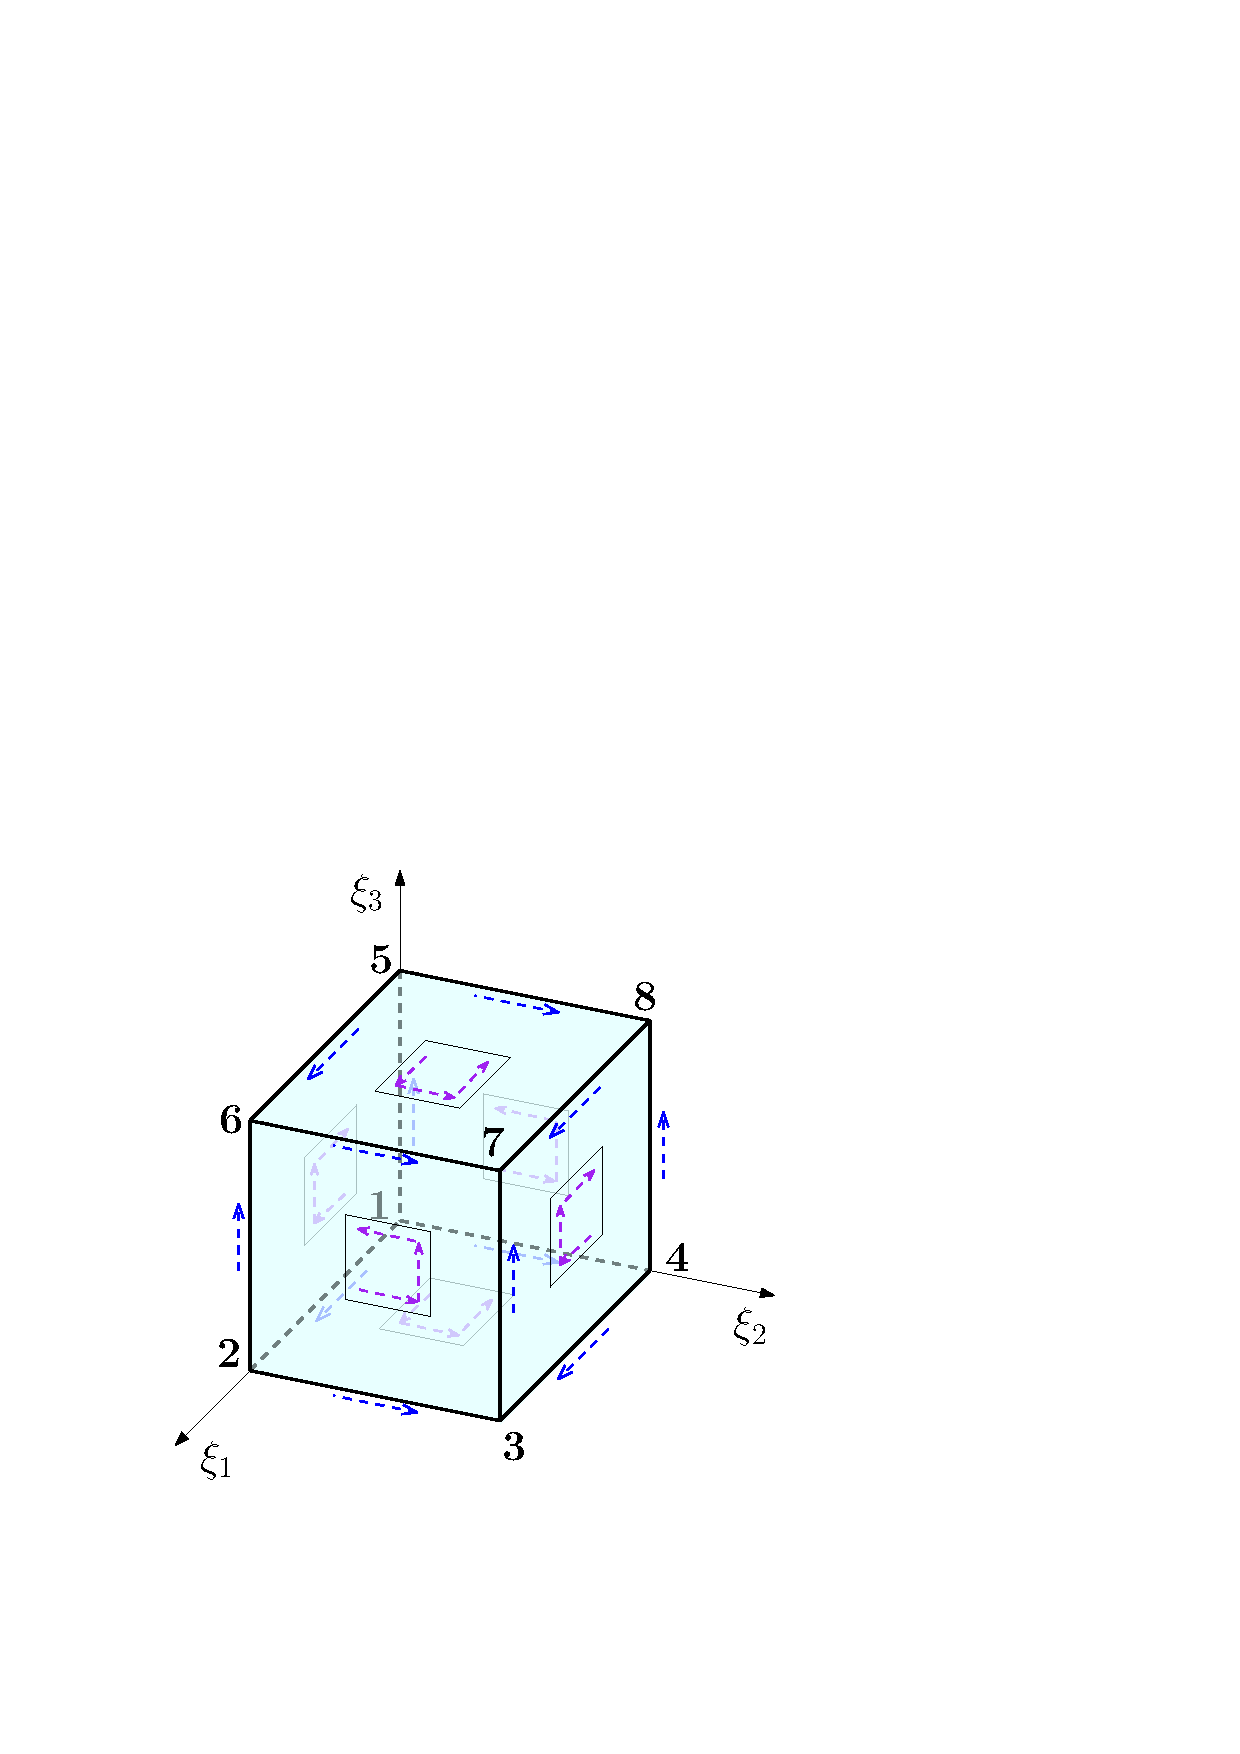
\includegraphics[scale=0.5]{./figures/MasterHexaOrientations.pdf}
\caption{Master hexahedron with numbered vertices \textit{and} local edge and face orientations.}
\label{fig:MasterHexaOrientations}
\end{center}
\end{figure}

Figure \ref{fig:MasterHexaOrientations} shows the master hexahedron along with a schematic representing all predefined \textit{local} edge and face orientations.
They represent the $\oo=0$ case.
They are \textit{our} choices for the local orientations (which in fact are the ``lexicographic'' orientations), but others may choose different local orientations to represent their $\oo=0$ case.

To find the locally ordered tuples, the key is being aware of the relationships between the vertices and the affine coordinates.
To illustrate this take as an example edge 12 and face 1234.

Edge 12 is composed of the vertices $v_1$ and $v_2$. 
Here, $v_1$ is linked to $\mu_0(\xi_1)$, $\mu_0(\xi_2)$,$\mu_0(\xi_3)$, while $v_2$ is linked to $\mu_1(\xi_1)$, $\mu_0(\xi_2)$ and $\mu_0(\xi_3)$.
The only difference between the the two vertices is that $v_1$ is linked to $\mu_0(\xi_1)$, while $v_2$ is linked to $\mu_1(\xi_1)$.
Now, the local orientation is represented by the local vertex-ordering $v_1\tdashto v_2$, so quite simply the locally ordered pair is $\vec{\mu}_{01}(\xi_1)=(\mu_0(\xi_1),\mu_0(\xi_1))$ (if the local ordering was $v_2\tdashto v_1$, then the pair would be $\vec{\mu}_{10}(\xi_1)$).
Hence, the orientation embedded edge 12 shape functions in $H^1$ with their gradient are
\begin{equation*}
	\begin{aligned}
		\phi_i^\mathrm{e}(\xi)&=\mu_0(\xi_3)\mu_0(\xi_2)\phi_i^\E(\sigma_\oo^\E(\vec{\mu}_{01}(\xi_1)))\,,\\
		\nabla\phi_i^\mathrm{e}(\xi)&=\mu_0(\xi_c)\mu_0(\xi_b)\nabla\phi_i^\E(\sigma_\oo^\E(\vec{\mu}_{01}(\xi_1)))
			+\phi_i^\E(\sigma_\oo^\E(\vec{\mu}_{01}(\xi_1)))\Big(\mu_0(\xi_3)\nabla\mu_0(\xi_2)+\mu_0(\xi_2)\nabla\mu_0(\xi_3)\Big)\,,
	\end{aligned}
\end{equation*}
where $i=2,\ldots,p$. 
The same applies to the $H(\mathrm{curl})$ edge 12 shape functions and their curl.
Clearly the approach is analogous with any other edge.

Face 1234 is composed of the vertices $v_1$, $v_2$, $v_3$ and $v_4$.
Here, the final goal is to find a locally ordered quadruple composed of two pairs.
The local vertex-ordering corresponding to the local orientation of face 1234 is $v_1\tdashto v_2\tdashto v_3\tdashto v_4$.
All one needs to do is to take the first two elements of the list, $v_1\tdashto v_2$, and the second and third components of the list, namely $v_2\tdashto v_3$.
The former will represent the \textit{first} pair in the quadruple, while the latter represent the \textit{second} pair in the quadruple.
Then one proceeds as if these where edges, so that $v_1\tdashto v_2$ is associated to $\vec{\mu}_{01}(\xi_1)$, while $v_2\tdashto v_3$ is associated to $\vec{\mu}_{01}(\xi_2)$.
Finally the locally ordered quadruple is then the ordered succession of these two pairs, $(\vec{\mu}_{01}(\xi_1),\vec{\mu}_{01}(\xi_2))$.
Hence, the orientation embedded face 1234 shape functions in $H^1$ with their gradient are
\begin{equation*}
	\begin{aligned}
		\phi_{ij}^\mathrm{f}(\xi)&=\mu_0(\xi_3)\phi_{ij}^\square(\sigma_\oo^\square(\vec{\mu}_{01}(\xi_1),\vec{\mu}_{01}(\xi_2)))\,,\\
		\nabla\phi_{ij}^\mathrm{f}(\xi)&=\mu_0(\xi_3)\nabla\phi_{ij}^\square(\sigma_\oo^\square(\vec{\mu}_{01}(\xi_1),\vec{\mu}_{01}(\xi_2)))
			+\phi_{ij}^\square(\sigma_\oo^\square(\vec{\mu}_{01}(\xi_1),\vec{\mu}_{01}(\xi_2)))\nabla\mu_0(\xi_3)\,,
	\end{aligned}
\end{equation*}
where $i=2,\ldots,p_a$, $j=2,\ldots,p_b$, where $(p_a,p_b)$ are the orders of the first and second coordinate pairs in the quadruple $\sigma_\oo^\square(\vec{\mu}_{01}(\xi_1),\vec{\mu}_{01}(\xi_2))$.
The same applies to the $H(\mathrm{curl})$ and $H(\mathrm{div})$ face 1234 shape functions and their differential forms.
Once again, the approach is analogous with any other face.
%Section 7
\newpage
\section{Tetrahedron}
\label{sec:Tet}

\begin{figure}[!ht]
\begin{center}
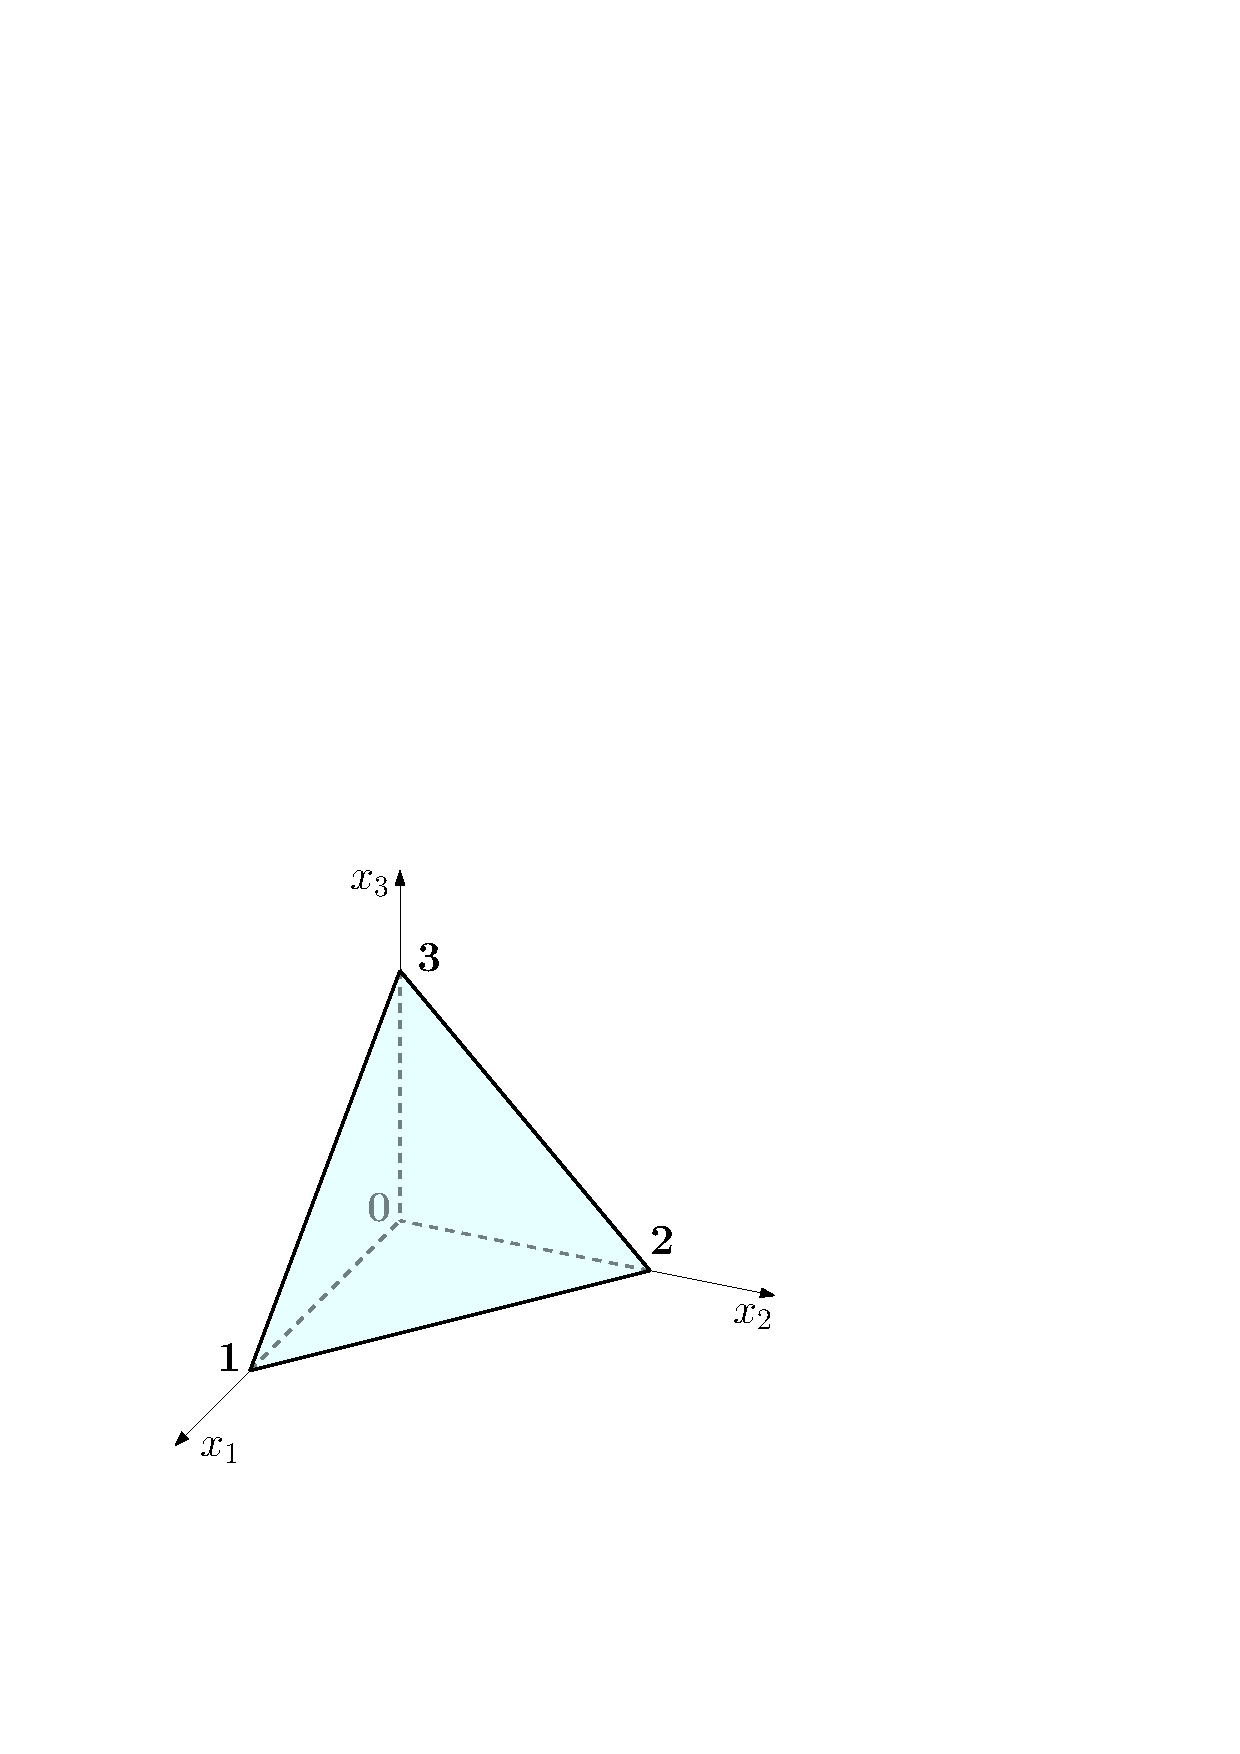
\includegraphics[scale=0.5]{./figures/MasterTet.pdf}
\caption{Master tetrahedron with numbered vertices.}
\label{fig:MasterTet}
\end{center}
\end{figure}

The 3D simplex is the tetrahedron. 
The master element for tetrahedra is illustrated in Figure \ref{fig:MasterTet} in the $x=(x_1,x_2,x_3)$ space.
More precisely, it is the set $\{x\in\R^3:x_1>0,x_2>0,x_3>0,x_1+x_2+x_3<1\}$.
%We shall denote the master tetrahedron by $\hat{\Tri}$ as well, as there will be no confusion with the triangle. The affine coordinates of the tetrahedron will be denoted by $\lambda_0,\lambda_1,\lambda_2,\lambda_3$. By ``edge $0-1$'' we mean the edge defined by $\lambda_0,\lambda_1$ and ``face $0-1-2$'' corresponds to the face defined by $\lambda_0,\lambda_1,\lambda_2$. Observe that
%\be
%\sum_{n=0}^d \lambda_n(x)=1\,,
%\ee
%and
%\be
%\lambda_n(x)\ge0\,,
%\ee
%for all $ x\in\hat\Tri$.

Denote vertex $a$ by $v_a$, so that $v_0=(0,0,0)$, $v_1=(1,0,0)$, $v_2=(0,1,0)$ and $v_3=(0,0,1)$.
As described in \S\ref{sec:affinecoordinates}, the 3D affine coordinates, $\lambda_0$, $\lambda_1$, $\lambda_2$ and $\lambda_3$, are easily calculated for this master tetrahedron:
\begin{equation}
	%\begin{aligned}
	\lambda_0(x)=1-x_1-x_2-x_3\,,\qquad
	\lambda_1(x)=x_1\,,\qquad
	\lambda_2(x)=x_2\,,\qquad
	\lambda_3(x)=x_3\,.
	%\begin{aligned}
\end{equation}
Their gradients are
\begin{equation}
	\nabla\lambda_0(x)=\bigg(\begin{smallmatrix}-1\\[2pt]-1\\[2pt]-1\end{smallmatrix}\bigg)\,,\qquad
	\nabla\lambda_1(x)=\bigg(\begin{smallmatrix}1\\[2pt]0\\[2pt]0\end{smallmatrix}\bigg)\,,\qquad
	\nabla\lambda_2(x)=\bigg(\begin{smallmatrix}0\\[2pt]1\\[2pt]0\end{smallmatrix}\bigg)\,,\qquad
	\nabla\lambda_3(x)=\bigg(\begin{smallmatrix}0\\[2pt]0\\[2pt]1\end{smallmatrix}\bigg)\,.
\end{equation}
These will be used explicitly or implicitly in what follows.

Just like the triangle and the segment, the tetrahedron has a very natural correspondence of its vertices and its affine coordinates.
Quite simply, each vertex $v_a$ is linked to the affine coordinate $\lambda_a$, for $a=0,1,2,3$.
Indeed, $\lambda_a$ takes the value $1$ at the associated vertex.

\subsubsection*{Exact Sequence}

As with the hexahedron, the tetrahedron will have a 3D discrete polynomial exact sequence that represents the continuous exact sequence \eqref{eq:3D_exact_sequence}. 
It is
\begin{equation}
\mathcal{P}^p\,\xrightarrow{\nabla}\,{\mathcal{N}}^p\,\xrightarrow{\nabla\times}\,{\mathcal{RT}}^p\,\xrightarrow{\nabla\cdot}
	\,\mathcal{P}^{p-1} \, ,
\end{equation}
where $\mathcal{P}^p =\mathcal{P}^p(x_1,x_2,x_3)$ is the space of polynomials of total order $p$.
Meanwhile, the N\'{e}d\'{e}lec and Raviart-Thomas spaces for the tetrahedron where already defined by \eqref{eq:NedelecSpace} and \eqref{eq:RaviartThomasSpace}, where $N=3$ in those definitions.

Like the triangle, the tetrahedron sequence has an overall drop in polynomial order of one, which makes it compatible with the construction of the hexahedron.
Also, as noted before, all of the spaces in the exact sequence are invariant under affine transformations. 

%Let $\mathcal{P}^p =\mathcal{P}^p(x_1,x_2,x_3)$ be the space of polynomials of total order $p$ in the $x=(x_1,x_2,x_3)$ space.
%%Define $\mathcal{P}^p = \mathcal{P}^p(\hat\Tri)$ to be the space of polynomials of order $p$ on $\hat\Tri$ and $\left(\mathcal{P}^p\right)^3 = \left(\mathcal{P}^p (\hat\Tri)\right)^3$ to be the triple Cartesian product of $\mathcal{P}^p$ with itself, i.e., vector space of 3-tuples of elements in $\mathcal{P}^p$. Furthermore, define $\tilde{\mathcal{P}}^{p} = \tilde{\mathcal{P}}^{p} (\hat\Tri)$ to be the subspace of homogeneous polynomials of order $p$ on $\hat\Tri$. The space $\left(\tilde{\mathcal{P}}^{p}\right)^d$ is defined similarly.
%%As was the case with the triangle element, it is our intent to reproduce the 3D exact sequence
%Recall the 3D exact sequence
%\begin{equation}
%H^1\,\xrightarrow{\nabla}\,H(\text{curl})\,\xrightarrow{\nabla\times}\,H(\text{div})\,\xrightarrow{\nab\cdot}\,L^2\,.
%\end{equation}
%The corresponding polynomial exact sequence is
%%\be
%%H^1 \, \xrightarrow{\bfnab} \, H(\text{curl}) \, \xrightarrow{\bfnab\times} \, H(\text{div}) \, \xrightarrow{\bfnab\cdot} \, L^2 \, ,
%%\ee
%%at the element level. It is well known that over polynomials, the maximal order exact sequence for the tetrahedron ($d=3$) is
%\begin{equation}
%\mathcal{P}^p\,\xrightarrow{\nabla}\,{\mathcal{N}}^p\,\xrightarrow{\bfnab\times}\,{\mathcal{RT}}^p\,\xrightarrow{\bfnab\cdot}
%	\,\mathcal{P}^{p-1} \, ,
%\end{equation}
%where the definition of the three dimensional N\'{e}d\'{e}lec and Raviart-Thomas spaces, $\mathcal{N}^p$ and $\mathcal{RT}^p$, are reminded next:
%\begin{align}
%	\mathcal{N}^p&=(\mathcal{P}^{p-1})^3\oplus\Big\{E\in(\tilde{\mathcal{P}}^{p})^3: x\cdot E(x)=0\,\text{ for all } 
%		x\in\R^3\Big\}\,,\\
%	\mathcal{RT}^p&=(\mathcal{P}^{p-1})^3\oplus\Big\{V\in(\tilde{\mathcal{P}}^{p})^3:V(x)=\phi(x)x
%		=\phi(x)\Big(\begin{smallmatrix}x_1\\x_2\\x_3\end{smallmatrix}\Big) \, \text{ with }\phi\in\tilde{\mathcal{P}}^{p-1}\Big\}\,.
%\end{align}
%Note the overall drop in polynomial order is one. This makes it compatible with the construction presented for the hexahedron. As before, all of the spaces in the exact sequences above are invariant under affine transformations.

%\be
%{\mathcal{N}}^p := \left(\mathcal{P}^{p-1}\right)^d\oplus\left\{E\in\left(\tilde{\mathcal{P}}^{p}\right)^d \, : \,  x\cdot E( x) = 0 \, \text{ for all }  x\right\} \, ,
%\ee
%and
%\be
%{\mathcal{RT}}^p := \left(\mathcal{P}^{p-1}\right)^d\oplus\left\{V\in\left(\tilde{\mathcal{P}}^{p}\right)^d \, : \,V(x) =  x\,\phi( x) \, \text{ where } \phi \in\tilde{\mathcal{P}}^{p-1}\right\} \, ,
%\ee
%denote the N\'ed\'elec and Raviart-Thomas spaces, respectively.
%\begin{remark}
%As before, all of the spaces in the exact sequences above are invariant under affine transformations. 
%Also, $\Tri$ denotes the tetrahedron in physical space.
%\end{remark}

\subsection{\texorpdfstring{$H^1$}{H1} Shape Functions}
%
%In three dimensions, the trace of $H^1$ functions is the value of the function itself along the boundary.
%Hence, vertex functions should vanish at all nonadjacent faces, edge functions should vanish at all nonadjacent faces, face functions should vanish at all other faces, and bubbles should vanish at all faces.

It will be clear that all the $\frac{1}{6}(p+3)(p+2)(p+1)$ shape functions lie in $\mathcal{P}^{p}$ and span the space.

The ideas in this section are completely parallel to those presented for the triangle (see \S\ref{sec:Tri}) but in three dimensions.
Therefore, the trace properties will not be analyzed in detail, since they follow analogously.

\subsubsection{\texorpdfstring{$H^1$}{H1} Vertices}

%Affine coordinates in three dimensions will be denoted by $\lambda_0$, $\lambda_1$, $\lambda_2$ and $\lambda_3$. They are written explicitly for our master triangle:
%\begin{equation}
%	%\begin{aligned}
%	\lambda_0(x)=1-x_1-x_2-x_3\,,\qquad
%	\lambda_1(x)=x_1\,,\qquad
%	\lambda_2(x)=x_2\,,\qquad
%	\lambda_3(x)=x_3\,.
%	%\begin{aligned}
%\end{equation}
%Their gradients are
%\begin{equation}
%	\nabla\lambda_0(x)=\bigg(\begin{smallmatrix}-1\\[2pt]-1\\[2pt]-1\end{smallmatrix}\bigg)\,,\qquad
%	\nabla\lambda_1(x)=\bigg(\begin{smallmatrix}1\\[2pt]0\\[2pt]0\end{smallmatrix}\bigg)\,,\qquad
%	\nabla\lambda_2(x)=\bigg(\begin{smallmatrix}0\\[2pt]1\\[2pt]0\end{smallmatrix}\bigg)\,,\qquad
%	\nabla\lambda_3(x)=\bigg(\begin{smallmatrix}0\\[2pt]0\\[2pt]1\end{smallmatrix}\bigg)\,.
%\end{equation}
%Take note of the above, since they will be used explicitly or implicitly in the computations of shape functions throughout this section.

%Let $ a_0,\ldots, a_d$, $d=3$, denote the vectices of $\hat\Tri$. Any point $ x\in\hat\Tri$ can be expressed as a convex combination of the vertices,
%\be
% x = \sum_{n=0}^3 \lambda_n a_n\, .
%\ee
%The weight functions, $\lambda_0,\ldots,\lambda_3$, give simplex affine (barycentric, area)coordinates for $\hat\Tri$ and correspond to its vertex shape functions.
%
%In terms of the local coordinates $x_1,x_2,x_3$, we have that
%\begin{equation}
%\begin{array}{ccc}
%\lambda_0(x) &=& 1-x_1-x_2-x_3\\
%\lambda_1(x) &=& x_1\\
%\lambda(x) &=& x_2\\
%\lambda(x) &=& x_3.
%\end{array}
%\end{equation}
%Also, we have
%\begin{equation}\nabla \lambda_0(x) = \left(
%\begin{array}{c}
%-1\\
%-1\\
%-1\\
%\end{array}
%\right),\\ \nabla \lambda_1(x) = \left(
%\begin{array}{c}
%1\\
%0\\
%0\\
%\end{array}
%\right),\\
%\nabla \lambda_2(x) = \left(
%\begin{array}{c}
%0\\
%1\\
%0\\
%\end{array}
%\right),\\
%\nabla \lambda_3(x) = \left(
%\begin{array}{c}
%0\\
%0\\
%1\\
%\end{array}
%\right) \end{equation}

The vertex shape functions and their gradients are simply the affine coordinates themselves,
\begin{equation}
	\phi^\mathrm{v}(x)= \lambda_a(x)\,,\qquad\quad
	\nabla\phi^\mathrm{v}(x)=\nabla\lambda_a(x)\,,
\end{equation}
for $a=0,1,2,3$.
There are a total of $4$ vertex functions (one for each vertex).
%and
%\begin{equation}
%\nabla \phi^\mathrm{v}(x) = %\phi^\vv(s_n(x)) =
%\nabla \lambda_a(x) \, , \quad a=0,1,2,3,
%\label{eq:H1_CountingSimplexVert_tet_2}
%\end{equation}
%where $\nabla \lambda_n(x)$ are as given earlier

%As was the case with the triangular element, we have that the vertex shape functions, being linear functions of the spatial variables, have the required $H^1$ conformity. 
%Again, by construction, the vertex shape functions have the required vanishing properties as well: $\lambda_a(x)$ vanishes at all nodes except node $a$ for $a=0,1,2,3$, and takes the value $1$ at node $a$. They behave linearly, making them compatible with neighbouring elements.

\subsubsection{\texorpdfstring{$H^1$}{H1}  Edges}

These are treated just like triangle edges. 
Hence, one can recur to $\phi_i^\E$ directly. 
Take for instance edge 01. In this case, the shape functions are simply
\begin{equation*}
      \phi_i^\mathrm{e}(x)=\phi_i^\E(\vec{\lambda}_{01}(x))
    	=\underbrace{(\lambda_0(x)+\lambda_1(x))^i}_{\text{blend}}
    		\underbrace{\phi_i^\E\Big(\underbrace{\textstyle{\frac{\lambda_0(x)}{\lambda_0(x)+\lambda_1(x)}},
    			\textstyle{\frac{\lambda_1(x)}{\lambda_0(x)+\lambda_1(x)}}}_{\text{project}}\Big)}_{\text{evaluate}}\,,
\end{equation*}
for $i=2,\ldots,p$. 
%so that $(\tilde{\mu}_0,\tilde{\mu}_1)=(\frac{\lambda_0}{\lambda_0+\lambda_1},\frac{\lambda_1}{\lambda_0+\lambda_1})$ are the projected 1D affine coordinates. Since $\tilde{\mu}_1(x)=\frac{x_1}{1-x_2-x_3}$, this implies there is a three dimensional projection of the form 
The projection being implied is
\begin{equation*}
	(x_1,x_2,x_3)\;\longmapsto\;(\textstyle{\frac{x_1}{1-x_3}},\textstyle{\frac{x_2}{1-x_3}},0)
		\;\longmapsto\;(\textstyle{\frac{x_1}{1-x_2-x_3}},0,0)\,.
\end{equation*}
It consists of finding the intersection $P''=(\frac{x_1}{1-x_2-x_3},0,0)$ of the edge with the projecting plane passing through the original point $P=(x_1,x_2,x_3)$ and the opposite nonadjacent edge.
It is illustrated in Figure \ref{fig:TetProjection}. 
Alternatively it can be interpreted in two steps.
First it is projected to a point $P'$ in an adjacent face, using the projecting line passing through $P$ and the disjoint vertex to the face.
Once in the face, it is projected again to the desired edge using the traditional \textit{two} dimensional triangle projection (see Figure \ref{fig:TriangleProjection}).

\begin{figure}[!ht]
\begin{center}
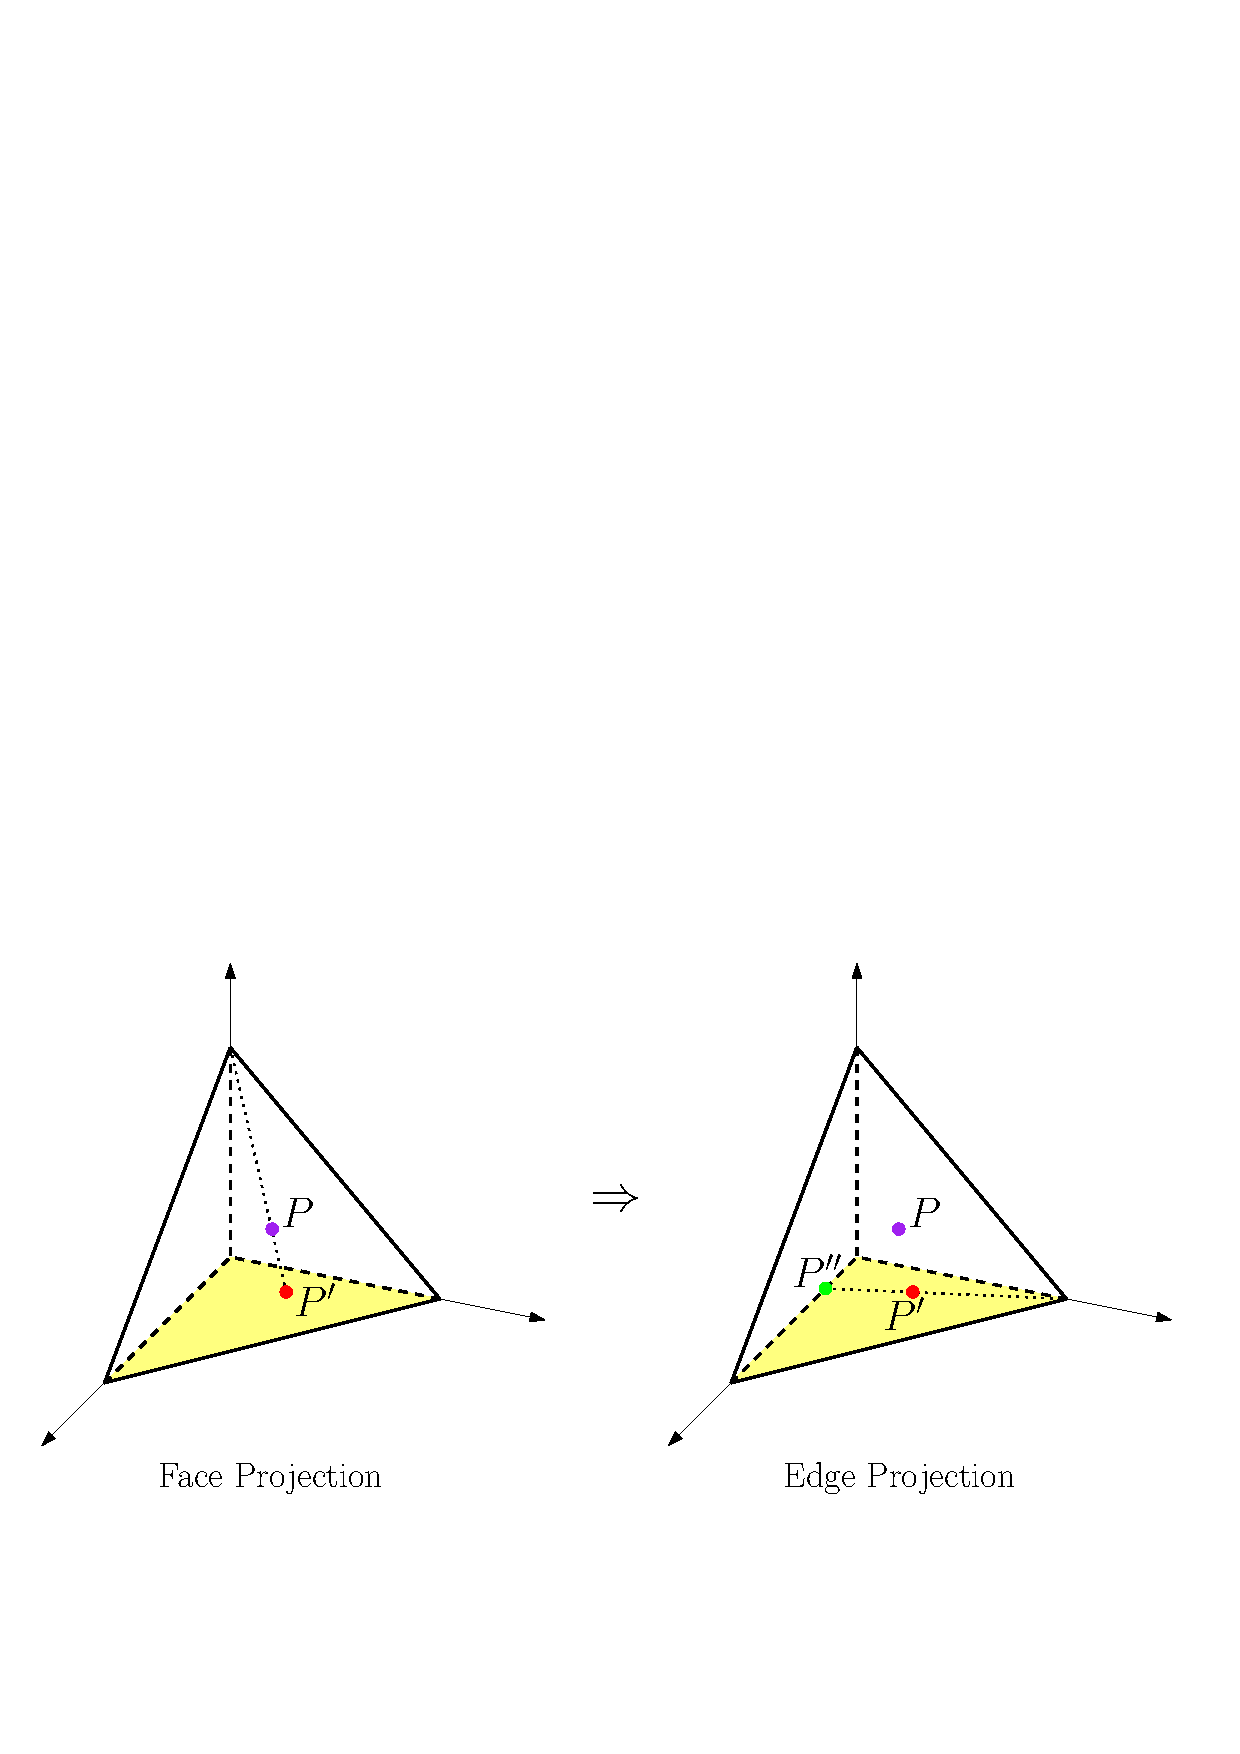
\includegraphics[scale=0.6]{./figures/TetProjection.pdf}
\caption{Face projection from $P$ to $P'$ followed by an edge projection from $P'$ to $P''$.}
\label{fig:TetProjection}
\end{center}
\end{figure}

More generally, the edge functions and their gradients are
\begin{equation}
	\phi_i^\mathrm{e}(x)=\phi_i^\E(\vec{\lambda}_{ab}(x))\,,\qquad\quad
		\nabla\phi_i^\mathrm{e}(x)=\nabla\phi_i^\E(\vec{\lambda}_{ab}(x))\,,
	\label{eq:Tetphigeneral}
\end{equation}
with $i=2,\ldots,p$, $0\leq a<b\leq3$. 
There are a total of $p-1$ edge functions for every given edge, leading to a total of $6(p-1)$ edge functions.

%For simplicity, we first consider the $0-1$ edge. Also, we consider the orientation $\oo=0$ case initially. As was the case with the triangular element, the map that associates a point in the tetrahedron the corresponding point on the edge with edge coordinates:
%\be
%\mu_n = \frac{\lambda_n}{\lambda_0+\lambda_1},\quad n=0,1\, ,
%\ee
%can be viewed as a projection onto the edge, whereas function
%$(\lambda_0 + \lambda_1)^i$ is the edge blending function.
%
%\begin{figure}[ht!]
%    \centering
%   % \begin{subfigure}[b]{0.45\textwidth}
%    %    \includegraphics[width=\textwidth]{./tri_V2.png}
%    %    \caption{Edge $H^1$ bubble for the triangle.}
%     %   \label{fig:H1edgebub_tri}
%    %\end{subfigure}%
%    ~ %add desired spacing between images, e. g. ~, \quad, \qquad, \hfill etc.
%      %(or a blank line to force the subfigure onto a new line)
%    \begin{subfigure}[b]{0.45\textwidth}
%        \includegraphics[width=\textwidth]{./figures/tet_V2.png}
%        \caption{Edge $H^1$ bubble projection for the tet.}
%    \end{subfigure}
%    \caption{Edge shape functions.}\label{fig:H1edgebub_tet}
%% \label{fig:H1bub_tri}
%\end{figure}

%We thus see that the edge function corresponding to the $0-1$ edge is $L_i(\lambda_1;\lambda_0+\lambda_1)$

%It follows from the construction that  $\phi^\E_i(\lambda_0,\lambda_1)$ satisfies the required vanishing property. Indeed, by construction, $\phi^\E_i(\lambda_0,\lambda_1)$ is nonzero on the $0-1$ edge and zero on the other two edges. Also, 
%\begin{equation}
%\phi^{\e,\oo}_i(\lambda_0,\lambda_1) = \nabla \phi^\E_i(\lambda_0,\lambda_1)
%\nonumber
%\end{equation}
% lies in the proper N\'ed\'elec space.


%With the above definition, we find that the $H^1$ edge shape functions are composed of the shape functions above, i.e., $\phi^\E_i$, considered on each edge independently;
%\be
%\phi^\mathrm{e}_i(x) = \phi^{\e}_i(\lambda_a(x),\lambda_b(x))% = \left[L_i\right](s_k,s_l)
% \, , \quad i=2,\ldots,p\, , \quad k<l=0,\ldots,3\,.
%\label{eq:H1_CountingSimplexEdge}
%\ee

%\paragraph{Edge Orientations}
%These are dealt with analogously to the triangular edge orientations as explained before. 
%This also applies to $H(\mathrm{curl})$ oriented edge shape functions.
%In order to incorporate the orientation embedding into the shape functions constructed in the above discussion, we modify the equations as follows (again, considering the $0-1$ edge as an example):
%\be
%\phi^{\e,\oo}_i(\lambda_0,\lambda_1) =
%\left\{
%    \begin{array}{ll}
%        \left[L_i\right](\lambda_0,\lambda_1) = L_i(\lambda_1;\lambda_0+\lambda_1) & \text{if } \oo = 0\\
%        \left[L_i\right](\lambda_1,\lambda_0) = L_i(\lambda_0;\lambda_1+\lambda_1) & \text{if } \oo = 1
%    \end{array}
%\right.
%\ee
% For simplicity, we have assumed unswapped coordinates in each case above.

% We leave it as a simple excercise for the reader to show that if we allow for $i=1$ in the definiton~\eqref{eq:H1_CountingSimplexEdge}, then $\phi_1(s_k,s_l)$ agrees with the vertex shape functions defined previously, albeit with some overcounting in the case of the tetrahedron.
% \textcolor{red}{Provide pictorial illustration of the projection in
% both 2D and 3D.}


% \textcolor{red}{Provide a pictorial example in 2D for an edge shape function}

\subsubsection{\texorpdfstring{$H^1$}{H1} Faces}

The construction of these shape functions follows simply by homogenizing the $H^1$ triangle face bubbles, since this will represent a polynomial extension preserving the desired vanishing properties.
This explains the definition of $\phi_{ij}^\Tri$ in terms of homogenized polynomials.
As an example, consider face 012, where the shape functions are
%In general, homogenization is the ideal tool to construct extensions for simplicial geometries
%To construct these shape functions, consider an $H^1$ triangle face bubble restricted to one face of the tetrahedron. For instance, take face 012, which corresponds to $\lambda_3=0$. Here, we already know the restriction of our shape function, which should be $\phi_{ij}^\Tri$. Homogenizing produces an $(i+j)$ order polynomial extension preserving the vanishing property on all other faces:
\begin{equation*}
	\phi_{ij}^\mathrm{f}(x)=\phi_{ij}^\Tri(\vec{\lambda}_{012}(x))=
		\underbrace{(\lambda_0(x)+\lambda_1(x)+\lambda_2(x))^{i+j}}_{\text{blend}}\underbrace{\phi_{ij}^\Tri
			\Big(\underbrace{\textstyle{\frac{1}{\lambda_0(x)+\lambda_1(x)+\lambda_2(x)}}
				\vec{\lambda}_{012}(x)}_{\text{project}}\Big)}_{\text{evaluate}}\,,
%	\phi_{ij}^\Tri(\lambda_0,\lambda_1,\lambda_2)=[L_i,L_j^{2i}](\lambda_0,\lambda_1,\lambda_2)
%		=(\lambda_0+\lambda_1+\lambda_2)^{i+j}[L_i,L_j^{2i}]
%			(\textstyle{\frac{\lambda_0}{\lambda_0+\lambda_1+\lambda_2}},\textstyle{\frac{\lambda_1}{\lambda_0+\lambda_1+\lambda_2}}
%				,\textstyle{\frac{\lambda_2}{\lambda_0+\lambda_1+\lambda_2}})\,.
\end{equation*}
for $i\geq2$ and $j\geq1$.
%Here, $(\tilde{\nu}_0,\tilde{\nu}_1,\tilde{\nu}_2)=(\frac{\lambda_0}{\lambda_0+\lambda_1+\lambda_2}, \frac{\lambda_1}{\lambda_0+\lambda_1+\lambda_2}, \frac{\lambda_2}{\lambda_0+\lambda_1+\lambda_2})$, are the projected two dimensional affine coordinates. 
%The projection is already illustrated in Figure \ref{fig:TetProjection} and has the form
%\begin{equation*}
%	(x_1,x_2,x_3)\;\longmapsto\;(\textstyle{\frac{x_1}{1-x_3}},\textstyle{\frac{x_2}{1-x_3}},0)\,.
%\end{equation*}
The projection is already illustrated in Figure \ref{fig:TetProjection} and consists of finding the intersection $P'=(\frac{x_1}{1-x_3},\frac{x_2}{1-x_3},0)$ of the face with the projecting line passing through the original point $P=(x_1,x_2,x_3)$ and the opposite vertex to the face. 
%This is illustrated in Figure \textit{add Figure}.

The full collection of shape functions and their gradient is
\begin{equation}
	\phi_{ij}^\mathrm{f}(x)=\phi_{ij}^\Tri(\vec{\lambda}_{abc}(x))\,,\qquad\quad
			\nabla\phi_{ij}^\mathrm{f}(x)=\nabla\phi_{ij}^\Tri(\vec{\lambda}_{abc}(x))\,,
			\label{eq:H1Tetfaces}
\end{equation}
where $i\geq2$, $j\ge1$, $n=i+j=3,\ldots,p$, and $0\leq a<b<c\leq3$. 
There are $\frac{1}{2}(p-1)(p-2)$ shape functions for each face, leading to a total of $2(p-1)(p-2)$ face functions.
%Homogenizing produces an $(i+j)$-order polynomial extension preserving the vanishing property on all other faces;
%\be
%\begin{array}{ll}
%\phi^\f_{ij}(\lambda_0,\lambda_1,\lambda_2) & = L_i\left(
%\frac{\frac{\lambda_1}{\lambda_0 + \lambda_1 + \lambda_2}}
%{\frac{\lambda_0}{\lambda_0 + \lambda_1 + \lambda_2}
%+\frac{\lambda_1}{\lambda_0 + \lambda_1 + \lambda_2}} \right)
%\left(
%\frac{\lambda_0 + \lambda_1}{\lambda_0 + \lambda_1 + \lambda_2} \right)^i
%L^{2i-1}_{j} \left(\frac{\lambda_2}{\lambda_0 + \lambda_1 + \lambda_2}\right)
%(\lambda_0 + \lambda_1 + \lambda_2)^{i+j} \\[20pt]
%& = L_i(\lambda_1; \lambda_0 + \lambda_1) L^{2i-1}_{j} (\lambda_2;
%\lambda_0 + \lambda_1 + \lambda_2)\\[12pt]
%& = \left[L_i,L^{2i-1}_{j}\right] (\lambda_0,\lambda_1,\lambda_2)\, .
%\end{array}
%\label{H1_TetHomog}
%\ee

%To construct the entire set of tetrahedron face bubbles, we must consider each face independently and so form the collection of shape functions
%\be
%\phi^\mathrm{f}_{ij}(x) = \phi^{\f}_{ij}(\lambda_a(x),\lambda_b(x),\lambda_c(x))% = \left[L_i,L^{2i-1}_{j}\right] (\lambda_k,\lambda_l,\lambda_m)\, ,%
%% \quad i\ge2,\, j\ge1, \, i+j=3,\ldots,p\, , \quad k<l<m=0,\ldots,3\,.
%\label{eq:H1_CountingTetFace}
%\ee
%% \be
%% \left\{\phi(x)\in\mathcal{P}^p(\hat\Tri) : \phi(x) = \phi^\f_{ij}(\lambda_k(x),\lambda_l(x),\lambda_m(x))\right\}
%% % \quad i\ge2,\, j\ge1, \, i+j=3,\ldots,p\, , \quad k<l<m=0,\ldots,3
%% \,,
%% \label{eq:H1_CountingTetFace}
%% \ee
%here, the indices range $i\ge2,\, j\ge1,\, i+j \leq p$, and $a\leq b \leq c \in\{0,1,2,3\}$.


%\paragraph{Face Orientations.}
%To consider orientations, simply take a predefined $\oo=0$ orientation for a given triangular face, and replace $\phi_{ij}^\Tri$ with $\phi_{ij}^{\Tri,\oo}$ (and similarly with the gradients). For instance, take face 123, which has a predefined local numbering of the vertices symbolized by $\xi^\mathrm{f}$ which goes from vertex 1 to vertex 2 to vertex 3. This defines the $\oo=0$ orientation and determines the order in which the entries should go in $\phi_{ij}^{\Tri,\oo}$. This way, for face 012, \eqref{eq:H1Tetfaces} becomes
%\begin{equation*}
%	\phi_{ij}^\mathrm{f}(x)=\phi_{ij}^{\Tri,\oo}(\lambda_1(x),\lambda_2(x),\lambda_3(x))\,,
%\end{equation*}
%with $i\geq2$, $j\ge1$, $n=i+j=3,\ldots,p$. The entries are then permuted according to orientation $\oo$ as described in \S\ref{sec:TriaFaceOrientations}. For this example, if $\oo=3$, it takes the form 
%\begin{equation*}
%	\phi_{ij}^\mathrm{f}(x)=\phi_{ij}^{\Tri,3}(\lambda_1(x),\lambda_2(x),\lambda_3(x))
%		=\phi_{ij}^\Tri(\lambda_1(x),\lambda_3(x),\lambda_2(x))\,,
%\end{equation*}
%with $i\geq2$, $j\ge1$, $n=i+j=3,\ldots,p$.

%To account for orientation embeddings, refer the reader to the permutation table defining $\sigma_{mathrm{o}}(\cdot)$ in the triangle section. With the permutation functions $\sigma_\oo$, $\oo=0,\ldots,5$ given in Figure~\ref{table:functionSigma}, we can fully define the affine $H^1$ face shape function for the $\lambda_3=0$ face of the tetrahedron
%\be
%\phi^{\f,\oo}_{ij}(\lambda_0,\lambda_1,\lambda_2) = \left[L_i,L^{2i-1}_{j}\right] (\lambda_{\sigma_\oo(0)},\lambda_{\sigma_\oo(1)},\lambda_{\sigma_\oo(2)})\,,
%\ee
%where $\oo=0,\ldots5$ denotes the given orientation of the affine coordinate system. The affine $H^1$ face shape function for all other faces are similarly defined.


\subsubsection{\texorpdfstring{$H^1$}{H1} Interior Bubbles}

The tetrahedron bubbles are given by blending a face shape function with a polynomial of complementing order which vanishes on the remaining face. 
As with triangles, it is carefully chosen as a Jacobi polynomial $L_k^{2(i+j)}$. 

The interior functions and their gradient are
\begin{equation}
	\begin{aligned}
		\phi_{ijk}^\mathrm{b}(x)&=\phi_{ij}^\Tri(\vec{\lambda}_{012}(x))[L_k^{2(i+j)}](\vec{\mu}_{01}(\lambda_3(x)))\,,\\
			\nabla\phi_{ijk}^\mathrm{b}(x)&=[L_k^{2(i+j)}](\vec{\mu}_{01}(\lambda_3(x)))\nabla\phi_{ij}^\Tri(\vec{\lambda}_{012}(x))
				+\phi_{ij}^\Tri(\vec{\lambda}_{012}(x))\nabla[L_k^{2(i+j)}](\vec{\mu}_{01}(\lambda_3(x)))\,,
	\end{aligned}
\end{equation}
%\begin{equation}
%\phi^\bb_{ijk}(\lambda_0,\lambda_1,\lambda_2,\lambda_3)
%&=  \phi^\f_{ij} (\lambda_0,\lambda_1,\lambda_2) \, \hat\phi_k(\lambda_3)
%\nonumber\\
%&= L_i(\lambda_1;\lambda_0+\lambda_1) L^{2i-1}_{j}
%(\lambda_2;\lambda_0+\lambda_1+\lambda_2) L^{2(i+j)-1}_{k} (\lambda_3)
%\nonumber\\
%&= \left[L_i,L^{2i-1}_{j},L^{2(i+j)-1}_{k}\right](\lambda_0,\lambda_1,\lambda_2,\lambda_3)
%\label{eq:H1_TetBubb}
%\end{equation}
where $i\geq2$, $j\geq1$, $k\geq1$ and $n=i+j+k=4,\ldots,p$, and where $\vec{\mu}_{01}(\lambda_3(x))=(1-\lambda_3(x),\lambda_3(x))$.
%Their gradients are
%\begin{equation}
%	\nabla\phi_{ijk}^\mathrm{b}(x)=L_k^{2(i+j)}(\lambda_3(x))\nabla\phi_{ij}^\Tri(\lambda_0(x),\lambda_1(x),\lambda_2(x))
%		+\phi_{ij}^\Tri(\lambda_0(x),\lambda_1(x),\lambda_2(x))P_{k-1}^{2(i+j)}(\lambda_3(x))\nabla\lambda_3(x)\,.
%\end{equation}
There are $\frac{1}{6}(p-1)(p-2)(p-3)$ interior shape functions in total.



%
%$$
%i \ge 2,\, j \ge 1,\, k \ge 1,\, i+j+k \leq p.
%$$ In the final line of Equation~\eqref{eq:H1_TetBubb}, we have used the property \mbox{$\sum\limits_{n=0}^3 \lambda_n = 1$}.
%
%The $H^1$ tetrahedron bubbles are defined
%\be
%\phi^\mathrm{b}_{ijk}(x) = \phi^\bb_{ijk}(\lambda_0(x),\lambda_1(x),\lambda_2(x),\lambda_3(x))\, ,
%\quad i \ge 2,\, j \ge 1,\, k \ge 1,\, i+j+k \leq p \, ,
%\label{eq:H1_CountingTetBubb}
%\ee
%for all $x\in\hat\Tri$.
%%
%\paragraph{\texorpdfstring{$H^1$}{H1} Linear Independence}
%
%To account for all of the constructed shape functions for the tetrahedron, we set $d=3$ and sum Equations~\eqref{eq:H1_CountingSimplexVert}, \eqref{eq:H1_CountingSimplexEdge}, \eqref{eq:H1_CountingTetFace}, \eqref{eq:H1_CountingTetBubb}. Accounting for the 4 vertices, 6 edges, and 4 faces, we have constructed
%\be
%4+6(p-1)+4{p-1\choose 2}+{p-1\choose 3} = {p+3\choose 3}
%\ee
%shape functions. Note that ${p+3\choose 3}$ is also the dimension of the polynomial space $\mathcal{P}^p$ in $\mathbb{R}^3$.
%
%The linear independence of the above shape functions, using the presented Lobatto and integrated Jacobi polynomials is given in \textit{cite Beuchler} and \textit{cite}.
%
%Since the cardinality of our set of linearly independent shape functions agrees with the dimension of $\mathcal{P}^p$ for the tetrahedron, we understand that our set is spanning and that we have constructed an appropriate basis for the space.

\subsection{\texorpdfstring{$H(\mathrm{curl})$}{Hcurl} Shape Functions}

%In three dimensions, the trace of $H(\mathrm{curl})$ functions is the tangential component of the vector function along the boundary.
%All edge functions should have vanishing trace at all other edges, and all face functions should have vanishing trace at all other faces, while the bubbles should have zero trace along all faces.

The dimension of $\mathcal{N}^p$ in three dimensions is $\frac{1}{2}p(p+2)(p+3)$.
A careful count of the linearly independent shape functions to be presented throughout this section will coincide with that dimension. 
Showing that the functions constructed are in $\mathcal{N}^p$ follows from Lemma \ref{lemma:curl}.
The constructions are all analogous to those of the triangle and simply require of an extra extension which is naturally provided by homogenization.
%We ask the reader to review the corresponding section of the triangle element. The constructions are all analogous and simply require of an extra extension which is naturally provided by homogenization.
%In particular, we shall be using the lemmata stated in that section for the $H(\text{curl})$ shape functions for the tetrahedron.

\subsubsection{\texorpdfstring{$H(\mathrm{curl})$}{Hcurl} Edges}

%Consider the $0-1$ edge of a tetrahedron. Here again, we no longer need an endpoint vanishing property for the edge shape functions. Without taking into account embedded orienations, for an edge with endpoint affine coordinates $0-1$, we define the affine $H(\text{curl})$ edge functions by:
%\be
%E^\E_i(\lambda_0,\lambda_1) = \left[\hat\psi_i\right](\lambda_0,\lambda_1)
%(\lambda_0 \bfnab \lambda_1 - \lambda_1 \bfnab \lambda_0 )\, , \quad i=0,\ldots,p-1\,.
%\label{eq:edge_curl_25}
%\ee
%If $\hat\psi_i = P_i$, where $P_i$ denotes the shifted scaled Legendre polynomial of order $i$, then clearly, $$\left[\hat\psi_i\right] = \left[P_i\right]\,,$$ and by Lemma~\ref{lemma:curl},
%\be
%\bfnab \times E_i^\E(\lambda_0,\lambda_1) =  (i+2) \, \left[P_i\right](\lambda_0,\lambda_1) \,
%\bfnab \lambda_0 \times \bfnab \lambda_1 \, .
%\ee
%
%The complete collection of $H(\text{curl})$ edge shape functions is generated by
%\be
%E^\mathrm{e}_i(x) = E_i^{\e}(\lambda_a(x),\lambda_b(x)), \quad i\leq p\,,
%\ee
%where we account for all edges by considering all $0\leq a \leq b\leq 3$.

%\paragraph{Orientation Considerations}
%Taking into account orientation changes on the edge, as before we have the following orientation embedded definitions for the affine $H(\text{curl})$ edge functions:
%\be
%E^{\e,\oo}_i(\lambda_0,\lambda_1) =
%\left\{
%    \begin{array}{ll}
%        \left[P_i\right](\lambda_0,\lambda_1)\left(\lambda_0 \bfnab \lambda_1 - \lambda_1 \bfnab \lambda_0\right) & \text{if } \oo =0 \\
%        \left[P_i\right](\lambda_1,\lambda_0)\left(\lambda_1 \bfnab \lambda_0 - \lambda_0 \bfnab \lambda_1\right) & \text{if } \oo =1
%    \end{array}
%\right.
%\ee

These are just the same as in the triangle case, but using three dimensional affine coordinates for the homogenization.
For example, for edge 01, the shape functions are
\begin{equation*}
	\begin{aligned}
		E_i^\mathrm{e}(x)&=E_i^\E(\vec{\lambda}_{01}(x))=
			[P_i](\vec{\lambda}_{01}(x))\Big(\lambda_0(x)\nabla\lambda_1(x)-\lambda_1(x)\nabla\lambda_0(x)\Big)\\
    	&=(\lambda_0(x)+\lambda_1(x))^i
    [P_i]\Big(\textstyle{\frac{\lambda_0(x)}{\lambda_0(x)+\lambda_1(x)}},\textstyle{\frac{\lambda_1(x)}{\lambda_0(x)+\lambda_1(x)}}\Big)
    			E_0^\E(\vec{\lambda}_{01}(x))\\
    	&=\underbrace{(\lambda_0(x)+\lambda_1(x))^{i+2}}_{\text{blend}}
    		\underbrace{E_i^\E\Big(\underbrace{\textstyle{\frac{\lambda_0(x)}{\lambda_0(x)+\lambda_1(x)}},
    			\textstyle{\frac{\lambda_1(x)}{\lambda_0(x)+\lambda_1(x)}}}_{\text{project}}\Big)}_{\text{evaluate}}\,,
	\end{aligned}
\end{equation*}
for $i=0,\ldots,p-1$.
Regarding the traces, note that they are completely inherited from $E_0^\E(\vec{\lambda}_{01}(x))$, which is a Whitney function known to have the desired vanishing properties and being tracewise compatible with the lower dimensional triangle edge functions.
Therefore, all trace properties are satisfied, including the nonzero decay along the adjacent faces to the edge.

The edge functions with their curl are
\begin{equation}
	E_i^\mathrm{e}(x)=E_i^\E(\vec{\lambda}_{ab}(x))\,,\qquad\quad
		\nabla\times E_i^\mathrm{e}(x)=\nabla\times E_i^\E(\vec{\lambda}_{ab}(x))\,,
	\label{eq:TetEgeneral}
\end{equation}
for $i=0,\ldots,p-1$, and $0\leq a<b\leq3$. 
There are a total of $p$ edge functions for every given edge, for a total of $6p$ edge functions.

\subsubsection{\texorpdfstring{$H(\mathrm{curl})$}{Hcurl} Faces}

%Take $p$ to be the order of $\lambda_3=0$ face of the tetrahedron and take $i \geq 0,\, j \geq 1,\, i+j\leq p-1$. Assume that we have orientation $\oo=0$ on this face. Recall the construction of the triangle $H(\text{curl})$ bubbles: $E^{\Tri\text{ ,I}}_{ij}(s_0(x),s_1(x),s_2(x))$ and $E^{\Tri\text{ ,II}}_{ij}(s_0(x),s_1(x),s_2(x))$. Introducing $s_i=\lambda_i, \text{ } i = 0,1,2,3,$ we arrive at the $H(\text{curl})$ tetrahedron face functions.

%Collecting all of the $H(\text{curl})$ tetrahedron face functions together, we have two families accounting for each of the four faces ($a,b,c = 0,1,2,3, \text{ }0 \leq a \leq b \leq c \leq 3$):
%\begin{description}
%  \item[Family I:]
%\be
%E^\mathrm{f}_{ij}(x) = E^{\f, \text{ I}}_{ij}(\lambda_a(x),\lambda_b(x),\lambda_c(x)),\quad i \geq 0,\, j \geq 1,\quad i+j=1,\ldots,p-1
%\ee
%
%  \item[Family II:]
%\be
%E^\mathrm{f}_{ij}(x) = E^{\f,\text{ II}}_{ij}(\lambda_a(x),\lambda_b(x),\lambda_c(x)),\quad i \geq 0,\, j \geq 1,\quad i+j=1,\ldots,p-1\,.
%\ee
%\end{description}

Like the triangle, the tetrahedron has two families of shape functions for every face.
The trace properties follow from those of the edge functions.
There is a grand total of $4p(p-1)$ face functions.

\subparagraph{Family I:} 
The shape functions and their curls are
\begin{equation}
	E_{ij}^{\mathrm{f}}(x)=E_{ij}^\Tri(\vec{\lambda}_{abc}(x))\,,\qquad\quad
		\nabla\times E_{ij}^{\mathrm{f}}(x)=\nabla\times E_{ij}^\Tri(\vec{\lambda}_{abc}(x))\,,
\end{equation}
for $i\geq0$, $j\geq1$, $n=i+j=1,\ldots,p-1$, and $0\leq a<b<c\leq3$. 
For every face, there are $\frac{1}{2}p(p-1)$ face functions in this family.

\subparagraph{Family II:}
The shape functions and their curls are
\begin{equation}
	E_{ij}^{\mathrm{f}}(x)=E_{ij}^\Tri(\vec{\lambda}_{bca}(x))\,,\qquad\quad
		\nabla\times E_{ij}^{\mathrm{f}}(x)=\nabla\times E_{ij}^\Tri(\vec{\lambda}_{bca}(x))\,,
\end{equation}
for $i\geq0$, $j\geq1$, $n=i+j=1,\ldots,p-1$, and $0\leq a<b<c\leq3$.
The only difference with the first family is that the entries are permuted to $\vec{\lambda}_{bca}(x)$ instead of $\vec{\lambda}_{abc}(x)$.
For every face, there are $\frac{1}{2}p(p-1)$ face functions in this family.

%\paragraph{Orientation Considerations}
%
%Accounting for orientations, we define the first family of orientated affine $H(\text{curl})$ tetrahedron face functions on the $\lambda_3=0$ face
%\be
%E^{\f,\oo}_{ij}(\lambda_0,\lambda_1,\lambda_2) = \left[P_i,L^{2i-1}_{j}\right](\lambda_{\sigma_\oo(0)},\lambda_{\sigma_\oo(1)},\lambda_{\sigma_\oo(2)})\left(\lambda_{\sigma_\oo(0)} \bfnab \lambda_{\sigma_\oo(1)} - \lambda_{\sigma_\oo(1)} \bfnab \lambda_{\sigma_\oo(0)}\right)\,.
%\ee
%The second family is obtained by rotating the affine coordinates one index, i.e. setting:
%$$
%\lambda_i := \lambda_{i+1},\quad i=0,1,2
%$$
%where $i+1 := \text{mod}(i+1,2)$.


\subsubsection{\texorpdfstring{$H(\mathrm{curl})$}{Hcurl} Interior Bubbles}

%As with $H^1$ bubbles these are obtained by blending a face shape function in $H(\mathrm{curl})$ with a polynomial of complementing order which vanishes on the remaining face. It is chosen as the Jacobi polynomial $L_k^{2(i+j)}$. Here, one must be careful about double counting. The bubbles are

The construction is completely analogous to that of $H^1$ in the sense that they are obtained by multiplying the face functions by the Jacobi polynomial $L_k^{2(i+j)}$.
One must attempt this for various possible permutations of the entries, but being careful to ensure that they are linearly independent.
Three families arise.

The interior bubbles and their curl are
\begin{equation}
	\begin{aligned}
		E_{ijk}^\mathrm{b}(x)&=[L_k^{2(i+j)}](\vec{\mu}_{01}(\lambda_d(x)))E_{ij}^\Tri(\vec{\lambda}_{abc}(x))\,,\\
		\nabla\!\!\times\! E_{ijk}^\mathrm{b}(x)&=[L_k^{2(i+j)}](\vec{\mu}_{01}(\lambda_d(x)))
			\nabla\!\!\times\! E_{ij}^\Tri(\vec{\lambda}_{abc}(x))
				\!+\!\nabla[L_k^{2(i+j)}](\vec{\mu}_{01}(\lambda_d(x)))\!\times\! E_{ij}^\Tri(\vec{\lambda}_{abc}(x))\,,
	\end{aligned}
\end{equation}
where $i\geq0$, $j\geq1$, $k\geq1$, $n=i+j+k=2,\ldots,p-1$ and $(a,b,c,d)=(0,1,2,3),(1,2,3,0),(2,3,0,1)$, and where $\vec{\mu}_{01}(\lambda_d(x))=(1-\lambda_d(x),\lambda_d(x))$.
There is a grand total of $\frac{1}{2}p(p-1)(p-2)$ interior shape functions.

%\begin{equation}
%	E_{ijk}^\mathrm{b}(x)=E_{ij}^{\Tri_I}(\lambda_a(x),\lambda_b(x),\lambda_c(x))L_k^{2(i+j)}(\lambda_d(x))\,,
%\end{equation}
% Their curls are
%\begin{equation}
%	\nabla\times E_{ijk}^\mathrm{b}(x)=L_k^{2(i+j)}(\lambda_d(x))\nabla\times E_{ij}^{\Tri_I}(\lambda_a(x),\lambda_b(x),\lambda_c(x))
%		+P_{k-1}^{2(i+j)}\nabla\lambda_d(x)\times E_{ij}^{\Tri_I}(\lambda_a(x),\lambda_b(x),\lambda_c(x))\,.
%\end{equation}


%Let $p$ be the order of $H^1$ element's middle node and take $i\geq 0,j\ge 1,\, k\ge 1,\, i+j+k=2,\ldots,p-1$. The construction of the $H(\text{curl})$ tetrahedron bubbles is similar as to has been seen previously in the other bubble functions. Since we need not worry about orientations, the first family of shape functions of order $i+j+k$, is simply given by:
%\be
%E^\mathrm{b}_{ijk}(x) = E^\bb_{ijk}(\lambda_0(x),\lambda_1(x),\lambda_2(x),\lambda_3(x)),
%\ee
%where
%\begin{align}
%E^\bb_{ijk}(\lambda_0,\lambda_1,\lambda_2,\lambda_3) &= E^\f_{ij}(\lambda_0,\lambda_1,\lambda_2)\,L^{2(i+j)-1}_{k}(\lambda_3)
%\nonumber\\
%& = \left[P_i,L^{2i-1}_{j},L^{2(i+j)-1}_{k}\right](\lambda_0,\lambda_1,\lambda_2,\lambda_3) (\lambda_0 \bfnab \lambda_1 - \lambda_1 \bfnab \lambda_0)\,.
%\end{align}
%
%Observe that the curl is readily computed
%\be
%\begin{array}{rl}
%\bfnab \times E^\bb_{ijk} & = \bfnab \times E^\f_{ij} (\lambda_0,\lambda_1,\lambda_2)\, L^{2(i+j)-1}_{k}(\lambda_3) + E^\f_{ij}(\lambda_0,\lambda_1,\lambda_2) \times \bfnab L^{2(i+j)-1}_{k}(\lambda_3)\\
%&= \bfnab \times E^\f_{ij} (\lambda_0,\lambda_1,\lambda_2)\, L^{2(i+j)-1}_{k}(\lambda_3)\\
%&\quad + \left[P_i,L^{2i-1}_j,P^{2(i+j)-1}_{k-1}\right](\lambda_0,\lambda_1,\lambda_2,\lambda_3)\,\left(\lambda_0 \bfnab \lambda_1 - \lambda_1 \bfnab \lambda_0\right)\times\bfnab\lambda_3\,.
%\end{array}
%\ee
%
%The second family and third families are obtained by rotating the affine coordinates, as we see in the following forumlas:
%\begin{description}
%  \item[Family I:]
%\be
%E^\mathrm{b}_{ijk}(x) = E^\bb_{ijk}(\lambda_0(x),\lambda_1(x),\lambda_2(x),\lambda_3(x)),\quad i\geq 0,j\ge 1,\, k\ge 1 \quad i+j+k=2,\ldots,p-1
%\ee
%
%  \item[Family II:]
%\be
%E^\mathrm{b}_{ijk}(x) = E^\bb_{ijk}(\lambda_1(x),\lambda_2(x),\lambda_3(x),\lambda_0(x)),\quad i\geq 0,j\ge 1,\, k\ge 1 \quad i+j+k=2,\ldots,p-1
%\ee
%
%  \item[Family III:]
%\be
%E^\mathrm{b}_{ijk}(x) = E^\bb_{ijk}(\lambda_2(x),\lambda_3(x),\lambda_0(x),\lambda_1(x)),\quad i\geq 0,j\ge 1,\, k\ge 1 \quad i+j+k=2,\ldots,p-1\,.
%\ee
%\end{description}



%\paragraph{\boldmath{$H(\text{curl})$} Linear Independence}
%
%Note that for the tetrahedron we have constructed
%\be
%6p+8{p\choose2}+3{p\choose3} = \frac{p(p+2)(p+3)}{2}
%\ee
%shape functions.


\subsection{\texorpdfstring{$H(\mathrm{div})$}{Hdiv} Shape Functions}

%In three dimensions, the trace of $H(\mathrm{div})$ functions is the tangential component of the vector function along the boundary.
%All face functions should have vanishing trace at all other faces, while the bubbles should have zero trace at all faces. 

The dimension of $\mathcal{RT}^p$ in three dimensions is $\frac{1}{2}p(p+1)(p+3)$.
A careful count of the linearly independent shape functions presented here will coincide with that dimension. 
Showing that the functions constructed are in $\mathcal{RT}^p$ is not immediate, but follows from the next lemma, which should be kept in mind.

\begin{lemma}
\label{lemma:div}
Let $x\in\R^N$ for $N=3$, and $f_n\in\mathcal{P}^n(x)$ be any polynomial of total order $n$ in the coordinates $x=(x_1,x_2,x_3)$. Given $s_0$, $s_1$ and $s_2$ affine coordinates in $\R^3$ $($or simply linear functions in $x$$)$, it follows that the Raviart-Thomas space of order $n+1$, $\mathcal{RT}^{n+1}$, contains the function 
\begin{equation*}
	f_n(\bcdot)\Big(s_0\nabla s_1\times\nabla s_2+s_1\nabla s_2\times\nabla s_0+s_2\nabla s_0\times\nabla s_1\Big)\in\mathcal{RT}^{n+1}\,.
\end{equation*}
\end{lemma}
\begin{proof}
Recall the definition of the Raviart-Thomas space in three dimensions,
\begin{equation*}
	\mathcal{RT}^p=(\mathcal{P}^{p-1})^3\oplus\Big\{V\in(\tilde{\mathcal{P}}^{p})^3:V(x)=\phi(x)x
		=\phi(x)\Big(\begin{smallmatrix}x_1\\x_2\\x_3\end{smallmatrix}\Big) \, \text{ with }\phi\in\tilde{\mathcal{P}}^{p-1}\Big\}\,.
\end{equation*}
Affine coordinates are linear functions in $x=(x_1,x_2,x_3)$, so that
\begin{equation*}
	s_k(x)=a_k+b_k\cdot x\,,
\end{equation*}
for $a_k\in\R$, $b_k\in\R^3$ and $k=0,1,2$. Then $\nabla s_k(x)=b_k$ and
\begin{align*}
	V(x)&=s_0(x)\nabla s_1(x)\times\nabla s_2(x)+s_1(x)\nabla s_2(x)\times\nabla s_0(x)+s_2(x)\nabla s_0(x)\times\nabla s_1(x)\\
		&=(a_0+b_0\cdot x)(b_1\times b_2)+(a_1+b_1\cdot x)(b_2\times b_0)+(a_2+b_2\cdot x)(b_0\times b_1)\\
		&=\underbrace{\Big(a_0(b_1\times b_2)+a_1(b_2\times b_0)+a_2(b_0\times b_1)\Big)}_{=A}
			+\underbrace{\Big(b_0\cdot(b_1\times b_2)\Big)x}_{=B(x)}\,,			
\end{align*}
where the last term follows from various identities. Clearly, $A\in(\mathcal{P}^0)^3=\R^3$ and $b_0\cdot(b_1\times b_2)\in\tilde{\mathcal{P}}^0=\R$, so that $B\in\{V\in(\tilde{\mathcal{P}}^{1})^3: V(x)=\phi(x)x\}$. Hence, $V\in\mathcal{RT}^1$.

Now, $f_n\in\mathcal{P}^n=\mathcal{P}^{n-1}\oplus\tilde{\mathcal{P}}^n$, for $n\geq1$ can always be decoupled into $f_n=f_{n-1}+\tilde{f}_n$, where $f_{n-1}\in\mathcal{P}^{n-1}$ and $\tilde{f}_n\in\tilde{\mathcal{P}}^n$. As a result
\begin{equation*}
	f_n(x)V(x)=f_n(x)A+f_{n-1}(x)B(x)+\tilde{f}_n(x)B(x)\,,
\end{equation*}
where it is clear $f_{n}A+f_{n-1}B\in(\mathcal{P}^n)^3$ and $\tilde{f}_nB\in\{V\in(\tilde{\mathcal{P}}^{n+1})^3: V(x)=\phi(x)x\}$. Therefore, $f_nV\in\mathcal{RT}^{n+1}$.
\end{proof}
%As with the previous section on $H(\text{curl})$ shape functions, we begin with a lemma.

%\begin{lemma}
%\label{lemma:div}
%Let $V$ be a vector-valued function defined on a tetrahedron, given by:
%\be
%V =
%f_n(\lambda_0,\lambda_1,\lambda_2)
%\,
%[\lambda_0 \, \bfnab \lambda_1 \times \bfnab \lambda_2 +
%\lambda_1 \, \bfnab \lambda_2 \times \bfnab \lambda_0 +
%\lambda_2 \, \bfnab \lambda_0 \times \bfnab \lambda_1 ]
%\ee
%where $\lambda_0,\lambda_1, \lambda_2$ are differentiable functions of the spatial coordinates, and $f_n(t_1,t_2,t_3)$ is a
%homogeneous polynomial of (total) order $n$ in $t_1,t_2,t_3$. Then,
%\be
%\bfnab \cdot V = (n+3) \,
%f_n(\lambda_0,\lambda_1,\lambda_2)
%\, (\bfnab \lambda_0 \times \bfnab \lambda_1) \cdot \bfnab \lambda_2 \, .
%\ee
%Moreover, if $\lambda_0,\lambda_1, \lambda_2$ are affine coordinates, then $V$ belongs to the Raviart-Thomas space of order $n$,
%\be
%V \in \mathcal{RT}^n% := \left\{  x\phi( x) \, : \, \phi \in\tilde{\mathcal{P}}^{n-1}\right\}.
%.
%\ee
%\end{lemma}
%\begin{proof}
%Let us assume
%\be
%f_n(\lambda_0,\lambda_1) = g_n\left(\frac{\lambda_0}{\lambda_0+\lambda_1+\lambda_2},\frac{\lambda_1}{\lambda_0+\lambda_1+\lambda_2},\frac{\lambda_2}{\lambda_0+\lambda_1+\lambda_2}\right)\left(\lambda_0+\lambda_1+\lambda_2\right)^n
%\ee
%for some differentiable function, $g_n\in\mathcal{P}^n$.
%
%Here, we see that
%\begin{align*}
%\bfnab \cdot V &= \bfnab \cdot f_n(\lambda_0,\lambda_1,\lambda_2)
%\,
%[\lambda_0 \, \bfnab \lambda_1 \times \bfnab \lambda_2 +
%\lambda_1 \, \bfnab \lambda_2 \times \bfnab \lambda_0 +
%\lambda_2 \, \bfnab \lambda_0 \times \bfnab \lambda_1 ]\\
%&= \bfnab \left( g_n\left(\frac{\lambda_0}{\lambda_0+\lambda_1+\lambda_2},\frac{\lambda_1}{\lambda_0+\lambda_1+\lambda_2},\frac{\lambda_2}{\lambda_0+\lambda_1+\lambda_2}\right)\left(\lambda_0+\lambda_1+\lambda_2\right)^n\right)\\
%&\quad \cdot \,
%[\lambda_0 \, \bfnab \lambda_1 \times \bfnab \lambda_2 +
%\lambda_1 \, \bfnab \lambda_2 \times \bfnab \lambda_0 +
%\lambda_2 \, \bfnab \lambda_0 \times \bfnab \lambda_1 ]\\
%&\quad + f_n(\lambda_0,\lambda_1,\lambda_2) \, \bfnab \cdot \,
%[\lambda_0 \, \bfnab \lambda_1 \times \bfnab \lambda_2 +
%\lambda_1 \, \bfnab \lambda_2 \times \bfnab \lambda_0 +
%\lambda_2 \, \bfnab \lambda_0 \times \bfnab \lambda_1 ]\\
%&= \bfnab g_n\left(\frac{\lambda_0}{\lambda_0+\lambda_1+\lambda_2},\frac{\lambda_1}{\lambda_0+\lambda_1+\lambda_2},\frac{\lambda_2}{\lambda_0+\lambda_1+\lambda_2}\right)\left(\lambda_0+\lambda_1+\lambda_2\right)^n\\
%&\quad \cdot \,
%[\lambda_0 \, \bfnab \lambda_1 \times \bfnab \lambda_2 +
%\lambda_1 \, \bfnab \lambda_2 \times \bfnab \lambda_0 +
%\lambda_2 \, \bfnab \lambda_0 \times \bfnab \lambda_1 ]\\
%&\quad + n f_n(\lambda_0,\lambda_1,\lambda_2)\left(\bfnab\lambda_0+\bfnab\lambda_1+\bfnab\lambda_2\right)\left(\lambda_0+\lambda_1+\lambda_2\right)^{-1}\\
%&\quad \cdot \,
%[\lambda_0 \, \bfnab \lambda_1 \times \bfnab \lambda_2 +
%\lambda_1 \, \bfnab \lambda_2 \times \bfnab \lambda_0 +
%\lambda_2 \, \bfnab \lambda_0 \times \bfnab \lambda_1 ]\\
%&\quad + 3f_n(\lambda_0,\lambda_1,\lambda_2) \, (\bfnab \lambda_0 \times \bfnab \lambda_1) \cdot \bfnab \lambda_2\\
%&= (n+3)\,f_n(\lambda_0,\lambda_1,\lambda_2) \, (\bfnab \lambda_0 \times \bfnab \lambda_1) \cdot \bfnab \lambda_2,
%\end{align*}
%since
%\be
%\bfnab g_n\left(\frac{\lambda_0}{\lambda_0+\lambda_1+\lambda_2},\frac{\lambda_1}{\lambda_0+\lambda_1+\lambda_2},\frac{\lambda_2}{\lambda_0+\lambda_1+\lambda_2}\right) \quad \perp  \quad [\lambda_0 \, \bfnab \lambda_1 \times \bfnab \lambda_2 +
%\lambda_1 \, \bfnab \lambda_2 \times \bfnab \lambda_0 +
%\lambda_2 \, \bfnab \lambda_0 \times \bfnab \lambda_1 ].
%\ee
%
%Now, let $ x = (x_1,x_2,x_3)$ be the Cartesian coordinates of $ x\in\hat\Tri$, $\{\bfe_i\}_{i=1}^3$ be the Euclidean basis for $\mathbb{R}^3$, and $\eps_{ijk}$, for $i,j,k=1,2,3$, be the Levi-Civita tensor in $\mathbb{R}^3$,. Then, with
%\be
%\lambda_m = a_m + \sum_{i=1}^3 b_{mi}x_i,
%\ee
%where $a_m,b_{mi}\in\mathbb{R}$, $m=1,2$, $i=1,2,3$ we find that
%\begin{align*}
%&\quad \lambda_0 \, \bfnab \lambda_1 \times \bfnab \lambda_2 +
%\lambda_1 \, \bfnab \lambda_2 \times \bfnab \lambda_0 +
%\lambda_2 \, \bfnab \lambda_0 \times \bfnab \lambda_1\\
%&=  \sum_{i,j,k=1}^3\eps_{ijk}\left(a_0b_{1j}b_{2k}+a_1b_{2j}b_{0k}+a_2b_{0j}b_{1k}\right)\bfe_i + \sum_{i,j,k,l=1}^3\eps_{ijk}\left(b_{0l}b_{1j}b_{2k}+b_{1l}b_{2j}b_{0k}+b_{2l}b_{0j}b_{1k}\right)x_l\bfe_i\\
%&=  \sum_{i,j,k=1}^3\eps_{ijk}\left(a_0b_{1j}b_{2k}+a_1b_{2j}b_{0k}+a_2b_{0j}b_{1k}\right)\bfe_i + \sum_{i,j,k=1}^3\eps_{ijk}\left(b_{0i}b_{1j}b_{2k}+b_{1i}b_{2j}b_{0k}+b_{2i}b_{0j}b_{1k}\right)x_i\bfe_i,
%\end{align*}
%where the final line follows from symmetries of $\eps_{ijk}$.
%
%This completes the proof of Lemma 2.
%
%\end{proof}


\subsubsection{\texorpdfstring{$H(\mathrm{div})$}{Hdiv} Faces}
%As we have done throughout the previous discussion of the tetrahedral element, we consider the face $\lambda_3=0$ with orienation $0$. The affine $H(\text{div})$ face shape functions are:
%\be
%V^\f_{ij}(\lambda_0,\lambda_1,\lambda_2) = \left[P_i,P^{2i-1}_j\right](\lambda_0,\lambda_1,\lambda_2)
%\left( \lambda_0\,  \bfnab \lambda_1 \times \bfnab \lambda_2 +
%       \lambda_1\,  \bfnab \lambda_2 \times \bfnab \lambda_0 +
%       \lambda_2\,  \bfnab \lambda_0 \times \bfnab \lambda_1 \right)
%\label{eq:face_div}
%\ee
%with
%$$
%i\geq 0,\, j\ge 0,\quad i+j=0,\ldots,p-1\,,
%$$
%where $p$ is the face order for the corresponding $H^1$ element.
%As was the case with triangle $H(\text{curl})$ face functions, we can use the above formula for $V^\f_{ij}(\lambda_0,\lambda_1,\lambda_2)$ as a motivation for the following, more general definition.

The general formula for these functions is motivated by the well known first order Whitney form for $H(\mathrm{div})$, along with the fact that the normal trace of the faces should span the two dimensional $L^2$ space. The general definition is presented next.

\begin{definition*}
Let $s_0$, $s_1$ and $s_2$ be arbitrary functions of some spatial variable in $\R^N$, with $N=3$, and denote by $p$ the order in the coordinate triplet $(s_0,s_1,s_2)$. Then
\begin{equation}
	V_{ij}^{\Tri}(s_0,s_1,s_2)=[P_i,P_j^{2i+1}](s_0,s_1,s_2)\Big(s_0\nabla s_1\times\nabla s_2
		+s_1\nabla s_2\times\nabla s_0+s_2\nabla s_0\times\nabla s_1\Big)\,,
\end{equation}
for $i=n-j$, $j=0,\ldots,n$ and $n=0,\ldots,p-1$ $($or equivalently $i\geq0$, $j\geq0$ and $n=i+j=0,\ldots,p-1$$)$. The divergence is
\begin{equation}
	\nabla\cdot V_{ij}^{\Tri}(s_0,s_1,s_2)=(i+j+3)[P_i,P_j^{2i+1}](s_0,s_1,s_2)\nabla s_0\cdot(\nabla s_1\times\nabla s_2) \,.
	\label{eq:VdeltaDiv}
\end{equation}
\end{definition*}

The formula for the divergence follows from the following lemma, because $[P_i,P_j^{2i+1}](s_0,s_1,s_2)$ is a homogeneous polynomial of total order $n=i+j$ in $s_0$, $s_1$ and $s_2$.

\begin{lemma}
\label{lem:divformula}
Let $\psi_n(s_0,s_1,s_2)\in\tilde{\mathcal{P}}^n(s_0,s_1,s_2)$ be a homogeneous polynomial of total order $n$ in $s_0$, $s_1$ and $s_2$, where $s_0$, $s_1$ and $s_2$ are arbitrary functions of some spatial variable in $\R^N$, with $N=3$. Then
\begin{equation*}
    \nabla\cdot\Big(\psi_n(s_0,s_1,s_2)(s_0\nabla s_1\times\nabla s_2
			+s_1\nabla s_2\times\nabla s_0+s_2\nabla s_0\times\nabla s_1)\Big)
				\!=\!(n+3)\psi_n(s_0,s_1,s_2)\nabla s_0\cdot(\nabla s_1\times\nabla s_2)\,.
\end{equation*}
\end{lemma}
\begin{proof}
Let $V_{00}^{\Tri}(s_0,s_1,s_2)=(s_0\nabla s_1\times\nabla s_2
			+s_1\nabla s_2\times\nabla s_0+s_2\nabla s_0\times\nabla s_1)$. First notice that
\begin{align*}
	\nabla\cdot \Big(s_0(\nabla s_1\times\nabla s_2)\Big)
		&=\nabla s_0\cdot(\nabla s_1\times\nabla s_2)
			+s_0\Big(\nabla s_2\cdot\nabla\times\nabla s_1-\nabla s_1\cdot\nabla\times\nabla s_2\Big)\\
		&=\nabla s_0\cdot(\nabla s_1\times\nabla s_2)\,,
\end{align*}
and similarly with $\nabla\cdot(s_1(\nabla s_2\times\nabla s_0))$ and $\nabla\cdot(s_2(\nabla s_1\times\nabla s_2))$. All of them result in a scalar triple product, which is invariant to cyclic permutations. It follows
\begin{equation*}
	\nabla\cdot V_{00}^{\Tri}(s_0,s_1,s_2)=3\nabla s_0\cdot(\nabla s_1\times\nabla s_2)\,.
\end{equation*}
Now, consider a monomial $s_0^as_1^bs_2^c$. Then
\begin{align*}
	\nabla(s_0^as_1^bs_2^c)\cdot V_{00}^{\Tri}(s_0,s_1,s_2)
		&=(as_0^{a-1}s_1^bs_2^c\nabla s_0+bs_0^as_1^{b-1}s_2^c\nabla s_1+cs_0^as_1^bs_2^{c-1}\nabla s_2)
			\cdot V_{00}^{\Tri}(s_0,s_1,s_2)\\
		&=as_0^{a-1}s_1^bs_2^cs_0\nabla s_0\cdot(\nabla s_1\times\nabla s_2)
			+bs_0^as_1^{b-1}s_2^cs_1\nabla s_1\cdot(\nabla s_2\times\nabla s_0)\\
				&\qquad\qquad\qquad\qquad\qquad\qquad\qquad\qquad+cs_0^as_1^bs_2^{c-1}s_2\nabla s_2\cdot(\nabla s_0\times\nabla s_1)\\
		&=(a+b+c)s_0^as_1^bs_2^c\nabla s_0\cdot(\nabla s_1\times\nabla s_2)\,.
\end{align*}
With these last two results it follows
\begin{equation*}
	\nabla\cdot\Big(s_0^as_1^bs_2^cV_{00}^{\Tri}(s_0,s_1,s_2)\Big)=(a+b+c+3)s_0^as_1^bs_2^c\nabla s_0\cdot(\nabla s_1\times\nabla s_2)\,.
\end{equation*}
Then observe that any homogeneous polynomial $\psi_n(s_0,s_1,s_2)$ is composed of monomials of the form $s_0^as_1^bs_2^c$ of \textit{fixed} total order $a+b+c=n$. The result immediately follows.
\end{proof}

The result in \eqref{eq:VdeltaDiv} is quite remarkable in the sense that, as required by the construction, there are no derivatives of $[P_i,P_j^{2i+1}](s_0,s_1,s_2)$ in the expression for the divergence. 
Although not used in this section, record the following useful remark which will be exploited when dealing with the prism and pyramid elements.
\begin{remark}
Let $\nu_0=1-\nu_1-\nu_2$, where $\nu_1$ and $\nu_2$ are arbitrary functions of some spatial variable in $\R^N$ with $N=3$, and where $p$ is the order in the coordinates $(\nu_0,\nu_1,\nu_2)$. Then for all $i\geq0$, $j\geq0$ and $n=i+j=0,\ldots,p-1$,
\begin{equation}
    V_{ij}^\Tri(\nu_0,\nu_1,\nu_2)=[P_i,P_j^{2i+1}](\nu_0,\nu_1,\nu_2)\nabla\nu_1\times\nabla\nu_2\,,
    	\quad\qquad \nabla\cdot V_{ij}^\Tri(\nu_0,\nu_1,\nu_2)=0\,.\label{eq:HdivtriangleRemark}
\end{equation}
\end{remark}

These functions are still represented by the same projection, and follow the logic of projecting, evaluating and blending.
For example, take face 012, so the shape functions are
\begin{equation*}
	V_{ij}^\mathrm{f}(x)=V_{ij}^\Tri(\vec{\lambda}_{012}(x))=
		\underbrace{(\lambda_0(x)+\lambda_1(x)+\lambda_2(x))^{i+j+3}}_{\text{blend}}\underbrace{V_{ij}^\Tri
			\Big(\underbrace{\textstyle{\frac{1}{\lambda_0(x)+\lambda_1(x)+\lambda_2(x)}}
				\vec{\lambda}_{012}(x)}_{\text{project}}\Big)}_{\text{evaluate}}\,,
\end{equation*}
for $i\geq0$ and $j\geq0$.
It can be readily checked that they satisfy the required vanishing properties by focusing on the lowest order function $V_{00}^\mathrm{f}(x)$.
Moreover, by Lemma \ref{lemma:div} it is clear $V_{ij}^\mathrm{f}\in\mathcal{RT}^{n+1}$ for $n=i+j$. 

More generally, the shape functions and their divergence are
\begin{equation}
	V_{ij}^\mathrm{f}(x)=V_{ij}^\Tri(\vec{\lambda}_{abc}(x))\,,\qquad\quad
		\nabla\cdot V_{ij}^\mathrm{f}(x)=\nabla \cdot V_{ij}^\Tri(\vec{\lambda}_{abc}(x))\,,
\end{equation}
where $i\geq0$, $j\geq0$, $n=i+j=0,\ldots,p-1$, and $0\leq a<b<c\leq3$. 
%It can be readily checked they satisfy the required vanishing properties, and by Lemma \ref{lemma:div} it is clear $V_{ij}^\mathrm{f}\in\mathcal{RT}^{n+1}$ for $n=i+j$. 
Clearly, for each face there are $\frac{1}{2}p(p+1)$ functions, giving a total of $2p(p+1)$ face functions.
%\begin{definition*} Given the bubble function $V^\f_{ij}(s_0(x),s_1(x),s_2(x))$ with arguments $s_0(x),s_1(x),s_2(x)$, the corresponding two sets of $H(\text{div})$ triangle bubbles are: \\$V^{\f, \text{ I}}_{ij}(s_0(x),s_1(x),s_2(x)) = V^\f_{ij}(s_0(x),s_1(x),s_2(x)) \\
%V^{\f, \text{ II}}_{ij}(s_0(x),s_1(x),s_2(x)) = V^\f_{ij}(s_1(x),s_2(x),s_0(x))$ \\
%where \be
%V^\f_{ij}(s_0,s_1,s_2) = \left[P_i,P^{2i-1}_j\right](s_0,s_1,s_2)
%\left( s_0\,  \bfnab s_1 \times \bfnab s_2 +
%       s_1\,  \bfnab s_2 \times \bfnab s_0 +
%       s_2\,  \bfnab s_0 \times \bfnab s_1 \right)
%\label{eq:face_div_1}
%\nonumber
%\ee
%\\\end{definition*}
% One may observe that restricted to this face, the normal component of $V^\f_{ij}$ reduces to:
% $$
% V^\f_{ij} \cdot n_f = \left[P_i\right](\lambda_0,\lambda_1) \, P^{2i-1}_j(\lambda_2) \, .
% $$
% If we introduce:
% $$
% f_n(\lambda_0,\lambda_1,\lambda_2) =
% \left[P_i\right](\lambda_0,\lambda_1) \, P^{2i-1}_j(\lambda_2) \, ,
% $$
% the relation between the homogenized polynomials and scaled Legendre polynomials is
% $$
% [f]_n(\lambda_0,\lambda_1,\lambda_2)
% = \left[P_i,P^{2i-1}_j\right] (\lambda_0,\lambda_1,\lambda_2) .
% $$
%Specializing the above formula for the case of affine coordinates ($s_i=\lambda_i$, $i=0,1,2,3$), we now collect the families of $H(\text{div})$ face shape functions for each face,
%\begin{description}
%  \item[Family I:]
%\be
%V^\mathrm{f}_{ij}(x) = V^{\f,\text{ I}}_{ij}(\lambda_a(x),\lambda_b(x),\lambda_c(x)),\quad i \geq 0,\, j \geq 0,\quad i+j=0,\ldots,p-1
%\ee
%
%  \item[Family II:]
%\be
%V^\mathrm{f}_{ij}(x) = V^{\f,\text{ II}}_{ij}(\lambda_a(x),\lambda_b(x),\lambda_c(x)),\quad i \geq 0,\, j \geq 0,\quad i+j=0,\ldots,p-1\,.
%\ee
%\end{description}
%
%Moreover, by Lemma~\ref{lemma:div},
%\be
%\bfnab \cdot V^{\f,\text{ I}}_{ij}(\lambda_0,\lambda_1,\lambda_2) = (i+j+3) \left[P_i,P^{2i-1}_j\right] (\lambda_0,\lambda_1,\lambda_2)
%\, (\bfnab \lambda_0 \times \bfnab \lambda_1) \cdot \bfnab \lambda_2 \, ,
%\ee
%is easily computed, and lies in the correct energy space. Similar calculations hold for $V^{\f,\text{ II}}_{ij}(\cdot,\cdot,\cdot)$.

%\paragraph{Orientation Considerations}
%
%We now consider orientation embedded face functions. Defining
%\[
%V^\f_{00}(\lambda_0,\lambda_1,\lambda_2) = \left( \lambda_0\,  \bfnab \lambda_1 \times \bfnab \lambda_2 +
%       \lambda_1\,  \bfnab \lambda_2 \times \bfnab \lambda_0 +
%       \lambda_2\,  \bfnab \lambda_0 \times \bfnab \lambda_1 \right)\,,
%\]
%we can easily define the oriented affine $H(\text{div})$ face shape functions for the $\lambda_3=0$ face,
%\be
%V^{\f,\oo}_{ij}(\lambda_0,\lambda_1,\lambda_2) = \left[P_i,P^{2i-1}_j\right](\lambda_{\sigma_\oo(0)},\lambda_{\sigma_\oo(1)},\lambda_{\sigma_\oo(2)})\,V^\f_{00}(\lambda_{\sigma_\oo(0)},\lambda_{\sigma_\oo(1)},\lambda_{\sigma_\oo(2)})\,,
%\ee
%where $\sigma_\oo$ is the permutation of indices defined in Table~\ref{table:functionSigma}, $\oo=0,\ldots,5$. Similar definitions follow for the other faces.

\subsubsection{\texorpdfstring{$H(\mathrm{div})$}{Hdiv} Interior Bubbles}

%These are obtained by taking the $H(\mathrm{div})$ face functions and combining them with a polynomial of complementing order which vanishes on the remaining face. 
The construction is just like in $H^1$ and $H(\mathrm{curl})$, and there are three resulting families to consider.
The polynomial chosen to vanish is the Jacobi polynomial, $L_k^{2(i+j+1)}$. 

The interior functions with their divergence are
\begin{equation}
	\begin{aligned}
		V_{ijk}^\mathrm{b}(x)&=[L_k^{2(i\!+\!j\!+\!1)}](\vec{\mu}_{01}(\lambda_d(x)))V_{ij}^\Tri(\vec{\lambda}_{abc}(x))\,,\\
		\nabla\!\!\cdot\! V_{ijk}^\mathrm{b}(x)&=[L_k^{2(i\!+\!j\!+\!1)}](\vec{\mu}_{01}(\lambda_d(x)))
			\nabla\!\!\cdot\! V_{ij}^\Tri(\vec{\lambda}_{abc}(x))
				\!+\!\nabla[L_k^{2(i\!+\!j\!+\!1)}](\vec{\mu}_{01}(\lambda_d(x)))\!\cdot\! V_{ij}^\Tri(\vec{\lambda}_{abc}(x))\,,
	\end{aligned}
\end{equation}
where $i\geq0$, $j\geq0$, $k\geq1$, $n=i+j+k=1,\ldots,p-1$ and $(a,b,c,d)=(0,1,2,3),(1,2,3,0),(2,3,0,1)$, and where $\vec{\mu}_{01}(\lambda_d(x))=(1-\lambda_d(x),\lambda_d(x))$.
%Their divergence is
%\begin{equation}
%	\nabla\cdot V_{ijk}^\mathrm{b}(x)=L_k^{2(i+j+1)}(\lambda_d(x))\nabla\cdot V_{ij}^{\Tri}(\lambda_a(x),\lambda_b(x),\lambda_c(x))
%		+P_{k-1}^{2(i+j+1)}\nabla\lambda_d(x)\cdot V_{ij}^{\Tri}(\lambda_a(x),\lambda_b(x),\lambda_c(x))\,.
%\end{equation}
There is a grand total of $\frac{1}{2}p(p-1)(p+1)$ interior shape functions.

%No longer needing to worry about orienations, we define three families of affine $H(\text{div})$ tetrahedron bubbles on the $\lambda_3=0$ face. Let $p$ be the order of the exact sequence and $i,j\geq 0,\, k \geq 1,\,i+j+k=1,\ldots,p-1$, then the first family is defined as follows:
%\begin{align}
%V^\bb_{ijk}(\lambda_0,\lambda_1,\lambda_2,\lambda_3) &= V^\f_{ij} (\lambda_0,\lambda_1,\lambda_2)\, L^{2(i+j)-1}_k(\lambda_3)\\
%&= \left[P_i,P_j^{2i-1},L^{2(i+j)-1}_k\right](\lambda_0,\lambda_1,\lambda_2,\lambda_3) V^\f_{00}(\lambda_0,\lambda_1,\lambda_2,\lambda_3)\,,
%\end{align}
%where $V^f_{ij}$ is the affine face shape vector-valued polynomial
%of order $i+j$ defined by \textit{reference}, and $L^{\alpha}_k$ is the integrated scaled Jacobi polynomial of order $k$ and weight $2(i+j)-1$.
%
%The corresponding divergence is easily computed
%\begin{align}
%\bfnab \cdot V^\bb_{ijk}(\lambda_0,\lambda_1,\lambda_2,\lambda_3) &= \bfnab \cdot V^\f_{ij} (\lambda_0,\lambda_1,\lambda_2)\, L^{2(i+j)-1}_k(\lambda_3)
%+ V^\f_{ij} (\lambda_0,\lambda_1,\lambda_2)\cdot P^{2(i+j)-1}_{k-1} (\lambda_3) \bfnab \lambda_3
%\nonumber\\
%&= \left((i+j+3)L^{2(i+j)-1}_k(\lambda_3) -(\lambda_0+\lambda_1+\lambda_2)P^{2(i+j)-1}_{k-1} (\lambda_3)\right)
%\nonumber\\
%&\quad+\left[P_i,P^{2i-1}_j\right](\lambda_0,\lambda_1,\lambda_2) (\bfnab \lambda_0 \times \bfnab \lambda_1) \cdot \bfnab \lambda_2
%\end{align}
%The next two families are defined by rotating affine coordinates.
%
%\begin{description}
%  \item[Family I:]
%\be
%V^\mathrm{b}_{ijk}(x) = V^\bb_{ijk}(\lambda_0(x),\lambda_1(x),\lambda_2(x),\lambda_3(x)),\quad i\geq 0,j\ge 0,\, k\ge 1 \quad i+j+k=1,\ldots,p-1
%\ee
%
%  \item[Family II:]
%\be
%V^\mathrm{b}_{ijk}(x) = V^\bb_{ijk}(\lambda_1(x),\lambda_2(x),\lambda_3(x),\lambda_0(x)),\quad i\geq 0,j\ge 0,\, k\ge 1 \quad i+j+k=1,\ldots,p-1
%\ee
%
%  \item[Family III:]
%\be
%V^\mathrm{b}_{ijk}(x) = V^\bb_{ijk}(\lambda_2(x),\lambda_3(x),\lambda_0(x),\lambda_1(x)),\quad i\geq 0,j\ge 0,\, k\ge 1 \quad i+j+k=1,\ldots,p-1\,.
%\ee
%
%\end{description}
%

%\paragraph{\boldmath{$H(\text{div})$} Linear Independence}
%
%% Note that for the triangle, the map
%% \be
%% \varphi(x,y)=(y,-x),
%% \ee
%% is bijective from ${\mathop\mathcal{P}\limits_\sim}^{p-1}\oplus{\mathop\mathcal{N}\limits_\sim}^p$ to ${\mathop\mathcal{P}\limits_\sim}^{p-1}\oplus{\mathop\mathcal{T}\limits_\sim}^p$ and so we need not consider $H(\text{div})$ for the triangle.
%
%For the tetrahedron we have constructed
%\be
%4{p+1\choose2}+3{p+1\choose3} = \frac{p(p+1)(p+3)}{2}
%\ee
%shape functions.

\subsection{\texorpdfstring{$L^2$}{L2} Shape Functions}
The $\frac{1}{6}p(p+2)(p+1)$ shape functions will clearly span $\mathcal{P}^{p-1}$.

\subsubsection{\texorpdfstring{$L^2$}{L2} Interior}

Similar to the construction of $L^2$ triangle functions, the $L^2$ interior functions for the tetrahedron are
\begin{equation}
	\begin{aligned}
		\psi_{ijk}^\mathrm{b}(x)&=[P_i](\lambda_0(x),\lambda_1(x))[P_j^{2i+1}](\lambda_0(x)\!+\!\lambda_1(x),\lambda_2(x))
			[P_k^{2(i+j+1)}](1\!-\!\lambda_3(x),\lambda_3(x))\\
		&=[P_i,P_j^{2i+1}](\vec{\lambda}_{012}(x))[P_k^{2(i+j+1)}](\vec{\mu}_{01}(\lambda_3(x)))
			(\nabla\lambda_1(x)\!\!\times\!\!\nabla\lambda_2(x))\!\cdot\!\nabla\lambda_3(x)\,,
	\end{aligned}
\end{equation}
where $i\geq0$, $j\geq0$, $k\geq0$, and $n=i+j+k=0,\ldots,p-1$, and where $\vec{\mu}_{01}(\lambda_3(x))=(1-\lambda_3(x),\lambda_3(x))$. There is a total of $\frac{1}{6}p(p+2)(p+1)$ interior functions.
%$$
%i,j,k \geq 0,\quad i+j+k=0,\ldots,p-1 \, .
%$$

%\paragraph{\texorpdfstring{$L^2$}{L2} Linear Independence}
%
%We clearly have
%\be
%{p+2\choose3}
%\ee
%shape functions for the tetrahedron.
%
%The verification that we have constructed a basis follows similarly from the $H^1$ case.

\subsection{Orientations}
\label{sec:TetOrientations}

\begin{figure}[!ht]
\begin{center}
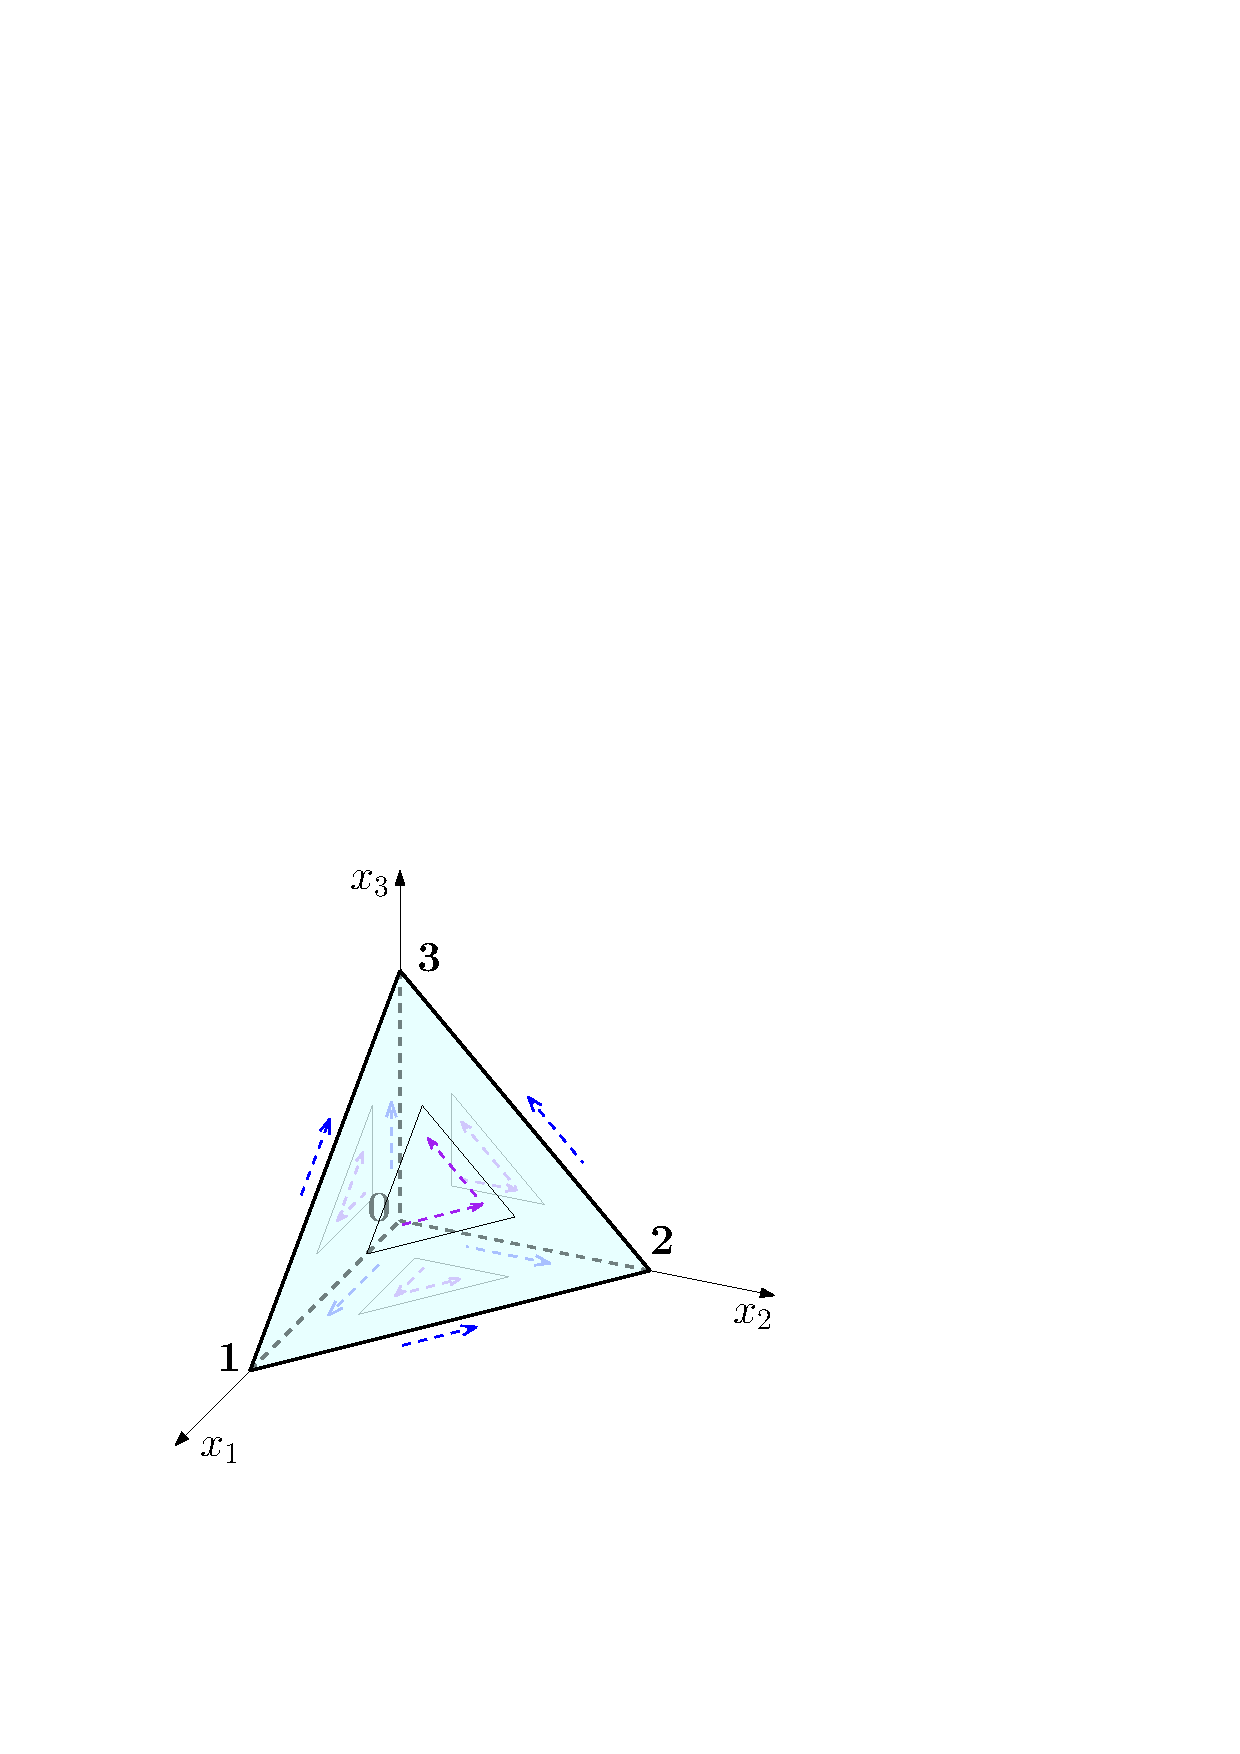
\includegraphics[scale=0.5]{./figures/MasterTetOrientations.pdf}
\caption{Master tetrahedron with numbered vertices \textit{and} local edge and face orientations.}
\label{fig:MasterTetOrientations}
\end{center}
\end{figure}

To construct orientation embedded shape functions for the tetrahedron, it is recommended to have read at least the first part of \S\ref{sec:HexaOrientations}.
The predefined \textit{local} edge and face orientations for the tetrahedron are illustrated in Figure \ref{fig:MasterTetOrientations}.
They represent the $\oo=0$ case.
The task at hand is to find the associated \textit{locally ordered} tuples of affine coordinates representing those local orientations.
As examples take edge 01 and face 012.

Edge 01 is composed of the vertices $v_0$ and $v_1$, which are linked uniquely to $\lambda_0$ and $\lambda_1$ respectively.
The local orientation for edge 01 is represented by the local vertex-ordering $v_0\tdashto v_1$.
As a result, the locally ordered pair for edge 01 is $\vec{\lambda}_{01}=(\lambda_0,\lambda_1)$.
It follows that the orientation embedded edge 01 shape functions in $H^1$ with their gradient are
\begin{equation*}
	\phi_i^\mathrm{e}(x)=\phi_i^\E(\sigma_\oo^\E(\vec{\lambda}_{01}(x)))\,,\qquad\quad
		\nabla\phi_i^\mathrm{e}(x)=\nabla\phi_i^\E(\sigma_\oo^\E(\vec{\lambda}_{01}(x)))\,,
\end{equation*}
with $i=2,\ldots,p$.
The same applies to the $H(\mathrm{curl})$ edge 01 shape functions and their curl.
The approach is analogous with any other edge.

Face 012 is composed of the vertices $v_0$, $v_1$ and $v_2$, which are linked to $\lambda_0$, $\lambda_1$ and $\lambda_2$ respectively.
The local orientation for the face is represented by the local vertex-ordering $v_0\tdashto v_1\tdashto v_2$, and as a result the locally ordered triplet for face 012 is $\vec{\lambda}_{012}=(\lambda_0,\lambda_1,\lambda_2)$.
Hence, for example the $H^1$ orientation embedded face 012 shape functions with their gradient are
\begin{equation*}
	\phi_{ij}^\mathrm{f}(x)=\phi_{ij}^\Tri(\sigma_\oo^\Tri(\vec{\lambda}_{012}(x)))\,,\qquad\quad
		\nabla\phi_{ij}^\mathrm{f}(x)=\nabla\phi_{ij}^\Tri(\sigma_\oo^\Tri(\vec{\lambda}_{012}(x)))\,,
\end{equation*}
with $i\geq2$, $j\geq1$ and $n=i+j=3,\ldots,p$.
The same applies to the $H(\mathrm{curl})$ and $H(\mathrm{div})$ face 012 shape functions and their differential forms.
Naturally, the approach is analogous with any other face.


%Section 8
\newpage
\section{Prism}
\label{sec:Prism}

\begin{figure}[!ht]
\begin{center}
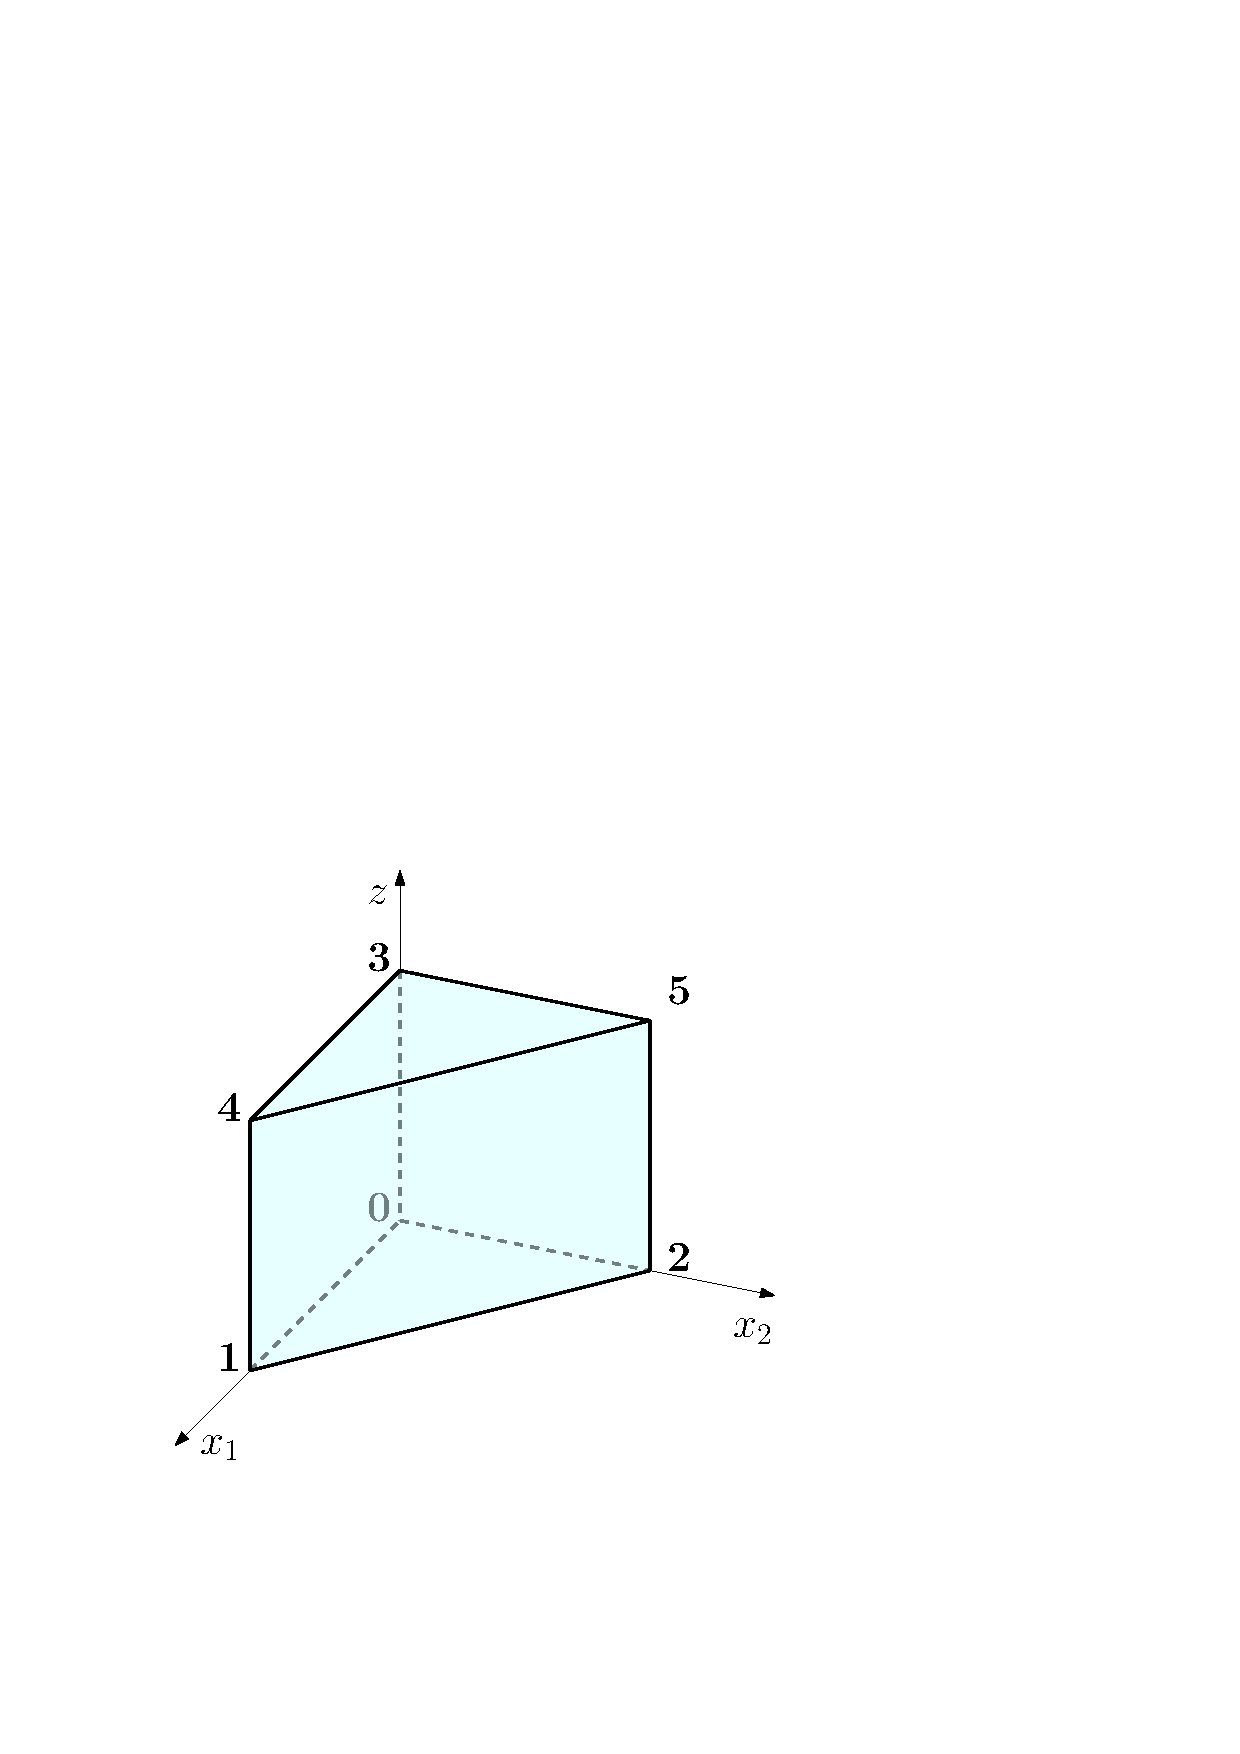
\includegraphics[scale=0.5]{./figures/MasterPrism.pdf}
\caption{Master prism with numbered vertices.}
\label{fig:MasterPrism}
\end{center}
\end{figure}

The master prism is shown in Figure \ref{fig:MasterPrism} in the $(x,z)=(x_1,x_2,z)$ space.
It is the Cartesian product of a triangle and a segment.
More specifically, it is $\{x\in\R^2:x_1>0,x_2>0,x_1+x_2<1\}\times(0,1)$.
Here, $x$ represents the triangle element coordinates, while $z$ represents the 1D segment element coordinate.

%The prism element can be viewed as the Cartesian product of the 2D triangle element and the 1D segment element. 
%The master element is shown in Figure \textit{addFig} in the $(x,z)$ space, where $x=(x_1,x_2)$. 
%Here, $x$ represents the triangle element coordinates, while $z$ represents the 1D segment element coordinate.

The prism has both quadrilateral and triangle faces. 
Similarly, there are two types of edges. 
Those edges which are adjacent to both a quadrilateral face and a triangle face are called \textit{mixed edges}, while those edges only shared by quadrilateral faces are simply called \textit{quadrilateral edges}. 
These distinctions are important, and the form of the shape functions will differ for the different types of edges and faces.

Due to the Cartesian product structure, it is natural to consider the 2D affine coordinates for the triangle (dependent on $x$) and the 1D affine coordinates for the segment (dependent on $z$). 
For this master element they are
\begin{equation}
	\begin{gathered}
		\nu_0(x)=1-x_1-x_2\,,\qquad\nu_1(x)=x_1\,,\qquad\nu_2(x)=x_2\,,\\
		\mu_0(z)=1-z\,,\qquad\quad\mu_1(z)=z\,.
	\end{gathered}
\end{equation}
Their gradients in 3D are
\begin{equation}
	\begin{gathered}
		\nabla\nu_0(x)=\bigg(\begin{smallmatrix}-1\\[2pt]-1\\[2pt]0\end{smallmatrix}\bigg)\,,\qquad
			\nabla\nu_1(x)=\bigg(\begin{smallmatrix}1\\[2pt]0\\[2pt]0\end{smallmatrix}\bigg)\,,\qquad
				\nabla\nu_2(x)=\bigg(\begin{smallmatrix}0\\[2pt]1\\[2pt]0\end{smallmatrix}\bigg)\,,\\
		\nabla\mu_0(z)=\bigg(\begin{smallmatrix}0\\[2pt]0\\[2pt]-1\end{smallmatrix}\bigg)\,,\qquad\quad
			\nabla\mu_1(z)=\bigg(\begin{smallmatrix}0\\[2pt]0\\[2pt]1\end{smallmatrix}\bigg)\,.
	\end{gathered}
\end{equation}
These are important and are used explicitly or implicitly in many of the oncoming calculations.

As usual, there are natural relationships between vertices, edges and faces, and the affine coordinates.
The related coordinates are those which take the value $1$ at the given topological entity.
In fact, for the prism each vertex is linked to \textit{two} affine coordinates, one of them a 2D affine coordinate and the other a 1D affine coordinate.
Moreover, each edge is linked to \textit{one} affine coordinate.
For mixed edges it is a 1D affine coordinate, while for quadrilateral edges it is a 2D affine coordinate.
Lastly, the triangle faces are also linked to \textit{one} 1D affine coordinate.
For example, vertex $0$, $v_0=(0,0,0)$, is linked to the affine coordinates $\nu_0(x)$ and $\mu_0(z)$.
Meanwhile, mixed edge 01 is linked to the affine coordinate $\mu_0(z)$, while quadrilateral edge 03 is linked to the affine coordinate $\nu_0(x)$.
Finally, face 012 is linked to $\mu_0(z)$.

\subsubsection*{Exact Sequence}

%Recall the 3D exact sequence
%\begin{equation*}
%H^1\,\xrightarrow{\nabla}\,H(\text{curl})\,\xrightarrow{\nabla\times}\,H(\text{div})\,\xrightarrow{\nabla\cdot}\,L^2\,.
%\end{equation*}
%
%As suggested by the structure of the prism, one would naturally expect the shape functions to be products or some combination of the corresponding shape functions of the triangle and segment element. 
%Indeed, this is the case. 
The product structure of the prism suggests that the discrete polynomial exact sequence approximating \eqref{eq:3D_exact_sequence} is intimately related to the discrete sequences for the triangle and segment (see \eqref{eq:EStriangle} and \eqref{eq:ESsegment}).
Indeed, this is the case. 
The sequence is of the form
%It is reflected as well in the discrete polynomial spaces in the exact sequence of the element, which are intricately related to the exact sequences for the triangle and line segment respectively (see \eqref{eq:EStriangle} and \eqref{eq:ESsegment}).
%Let $\mathcal{P}^p =\mathcal{P}^p(x_1,x_2)$ be the space of polynomials of total order $p$ in the $x=(x_1,x_2)$ space, and $\mathcal{P}^q=\mathcal{P}^q(z)$ be the space of polynomials of order $q$ in the $z$ variable. 
%Similarly, recall the definitions of the spaces $\mathcal{N}^p$ and $\mathcal{RT}^p$ in $N=2$ spatial dimensions given in \eqref{eq:NedelecSpace} and \eqref{eq:RaviartThomasSpace} which are assumed to be in the $x=(x_1,x_2)$ space. 
%Then, the finite dimensional exact sequence is of the form 
\begin{equation}
	W^{p,q} \xrightarrow{\,\,\nabla\,\,} Q^{p,q} \xrightarrow{\nabla\times} V^{p,q} \xrightarrow{\nabla\cdot} Y^{p,q} \,,
\end{equation}
where
\begin{equation}
	\begin{aligned}
	W^{p,q}&=\mathcal{P}^p\otimes\mathcal{P}^q=\mathcal{P}^p(x_1,x_2)\otimes\mathcal{P}^q(z)\,,\\
	Q^{p,q}&=(\mathcal{N}^p\otimes\mathcal{P}^q)\times(\mathcal{P}^p\otimes\mathcal{P}^{q-1})\,,\\
	V^{p,q}&=(\mathcal{RT}^p\otimes\mathcal{P}^{q-1})\times(\mathcal{P}^{p-1}\otimes\mathcal{P}^q)\,,\\
	Y^{p,q}&=\mathcal{P}^{p-1}\otimes\mathcal{P}^{q-1}\,.
	\end{aligned}
\end{equation}
Here, the spaces $\mathcal{N}^p$ and $\mathcal{RT}^p$ correspond to the $N=2$ case (see \eqref{eq:NedelecSpace} and	\eqref{eq:RaviartThomasSpace}), so that the space $\mathcal{N}^p\otimes\mathcal{P}^q=\{\phi E:\phi\in\mathcal{P}^q,E\in\mathcal{N}^p\}$ has two components and dimension $p(p+2)(q+1)$. The same applies to $\mathcal{RT}^p\otimes\mathcal{P}^{q-1}$ which has dimension $p(p+2)q$.


% will be an extension of the corresponding analysis of the triangle and line segment elements. 
%We will denote by $\hat{\Tri}$ the master triangle element, by $\hat{\mathrm{E}} $ the master line segment element, and by $\hat{\Lambda}$ the master prismatic element given as: \begin{equation} \hat{\Lambda} = \hat{\Tri} \times \hat{\mathrm{E}}\end{equation}

%Recall that the affine coordinate functions for the segment are denoted by $\mu_0, \mu_1$ \begin{equation}\mu_1(z)=z, \mu_0(z)=1-z, \mu_0+\mu_1=1 \end{equation} and for the triangle are denoted by \begin{equation}\nu_0(x,y)=1-x-y,\,\nu_1(x,y)=x,\,\nu_2(x,y)=y, \text{ with }\nu_0(x,y)+\nu_1(x,y)+\nu_2(x,y)=1.\end{equation}We will be needing the gradients (in 3D) of the above functions, which we record here: \begin{equation}\nabla \mu_1(z)=(0,0,1)^T,\text{ } \nabla \mu_0(z)= (0,0,-1)^T \end{equation}and \begin{equation}\nabla \nu_0(x,y) = \left(
%\begin{array}{c}
%-1\\
%-1\\
%0 \\
%\end{array}
%\right),\\ \nabla \nu_1(x,y) = \left(
%\begin{array}{c}
%1\\
%0\\
%0 \\
%\end{array}
%\right),\\
%\nabla \nu_2(x,y) = \left(
%\begin{array}{c}
%0\\
%1\\
%0\\
%\end{array}
%\right). \end{equation}
%The prism consists of two triangle faces, of which the ``top" face corresponds to $z=1$ and the ``bottom" face corresponds to $z=0$. We shall henceforth denote the arguments of all shape functions defined on the triangle element as $(x,y)$ and the argument of shape functions defined on the segment will be $z$, so that, for example, the affine function $\nu_0$ defined on the triangle will be written as $\nu_0(x,y)$ while the affine function defined $\mu_0$ on the interval as $\mu_0(z)$. This seperation of variables will allow us to see the tensor product structure more clearly.

%\subsubsection*{Exact Sequences for the Prismatic Element}
%Recall the exact sequence for the triangle element given by the N\'{e}d\'{e}lec/Raviart-Thomas characterization:
%\begin{equation}
%\begin{array}{ccccc} 
%\mathcal{P}^p(\hat{\Tri}) & \stackrel{\nabla}{\longrightarrow} & \mathcal{N}^p & \stackrel{\text{curl(}\cdot{)}}{\longrightarrow}\mathcal{P}^{p-1}(\hat{\Tri})\\ 
%\end{array},\end{equation}
%and,
%\begin{equation}
%\begin{array}{ccccc} 
%\mathcal{P}^p(\hat{\Tri}) & \stackrel{\nabla \times}{\longrightarrow} & \mathcal{R}\mathcal{T}^p & \stackrel{\nabla \cdot}{\longrightarrow}\mathcal{P}^{p-1}(\hat{\Tri})\\ 
%\end{array},\end{equation}
%where the spaces $\mathcal{N}^p$ and $\mathcal{R}\mathcal{T}^p$ are characterized by \begin{equation}\mathcal{N}^p := (\mathcal{P}^{p-1})^{2}\oplus\{ E\in (\tilde{\mathcal{P}^p})^{2}:{x}\cdot E(x)=0 \text{ } \forall x\}\end{equation}
%and \begin{equation}\mathcal{R}\mathcal{T}^p = (\mathcal{P}^{p-1})^{2}\oplus\{ {x}\phi({x}): \phi \in \tilde{\mathcal{P}}^{p-1}\}\end{equation} and are the N\'{e}d\'{e}lec and Raviart-Thomas spaces respectively. Following the presentation in , we have the following exact sequence for the prismatic element: 
%\begin{equation}\begin{array}{ccccc} 
%{W}^{p,q} & \stackrel{\nabla}{\longrightarrow} & {{Q}}^{p,q} & \stackrel{\nabla\times}{\longrightarrow}{V}^{p,q} & \stackrel{\nabla\cdot}{\longrightarrow}{Y}^{p,q}\\ 
%\end{array}, \end{equation}
%where we have:
%\begin{eqnarray}
% {W}^{p,q} &=& \mathcal{P}^p\otimes\mathcal{P}^q      \nonumber \\
% {Q}^{p,q} &=& (\mathcal{N}^p\otimes(\mathcal{P}^q\times\mathcal{P}^q))\times(\mathcal{P}^p\otimes\mathcal{P}^{q-1}) \nonumber \\
%  {V}^{p,q} &=& (\mathcal{RT}^p\otimes(\mathcal{P}^{q-1}\times\mathcal{P}^{q-1}))\times(\mathcal{P}^{p-1}\otimes\mathcal{P}^q) \nonumber \\
%  {Y}^{p,q} &=& \mathcal{P}^{p-1}\otimes\mathcal{P}^{q-1}.
%\end{eqnarray}
%We now discuss the shape functions for the prismatic element.

\subsection{\texorpdfstring{$H^1$}{H1} Shape Functions}
It will be clear that all shape functions lie in $\mathcal{P}^p\otimes\mathcal{P}^q$, which has dimension $\frac{1}{2}(p+2)(p+1)(q+1)$. 
Moreover, a judicious count of the shape functions constructed in this section coincides with that dimension, ensuring that the span of these is precisely $\mathcal{P}^{p}\otimes\mathcal{P}^q$.

Notice that for the triangle there are $H^1$ vertex, edge \textit{and} face shape functions, while for the segment there are $H^1$ vertex and edge functions. 
The six possible tensor products of these will precisely give the $H^1$ shape functions for the prism.
The vanishing properties are naturally inherited from each of the components of the tensor product structure of the shape functions, so they follow easily.

\subsubsection {\texorpdfstring{$H^1$}{H1} Vertices}
\label{sec:PrismH1vertices}

As usual with Cartesian product structures, the vertex functions are simply the product of the affine coordinates associated to the given vertex. 
Hence, they are the tensor product of lower dimensional vertex functions which inherit all the desired vanishing properties and the decays along adjacent faces to the vertex.
%of the prism, it is natural to expect that the $H^1$ vertex functions for the prism will be expressed as tensor products of the corresponding $H^1$ vertex functions of the triangle and segment elements. Indeed this is the case. 

The vertex shape functions and their gradients are
\begin{equation} 
	\begin{aligned}	
		\phi^\mathrm{v}(x,z)&=\nu_a(x)\mu_c(z)\,,\\
		\nabla\phi^\mathrm{v}(x,z)&=\mu_c(z)\nabla\nu_a(x)+\nu_a(x)\nabla\mu_c(z)\,,
	\end{aligned}		
\end{equation}
where $a=0,1,2$ and $c=0,1$. 
Notice $c=0$ represents the ``bottom'' face (vertices 0, 1 and 2), while $c=1$ represents the ``top'' face (vertices 3, 4 and 5).
Also $\nu_a$ represents vertices $a$ and $a+3$. 
There is a total of $6$ vertex functions (one for each vertex).

%The vanishing properties are easily seen to be satisfied, while the linear vertex blending towards adjacent edges and faces produced by $\nu_a(x)$ and $\mu_c(z)$ is also observed.
%These properties make the shape function compatible with potential adjacent elements.

%However, we have two sets of vertices, the ``bottom" vertices corresponding to the case $z=0$ with $z\in \hat{E}$ and the ``top" vertices corresponding to the case $z=1, z\in \hat{E}$. All together, we have $6$ vertices for the prismatic element. Thus, the $H^1$ vertex shape functions corresponding to the six vertices of $\hat{\Lambda}$ are given as the product of the triangle vertex functions and 1D vertex functions: \begin{equation}\phi^\mathrm{v}(x,y,z)=\nu_{a}(x,y)\mu_c(z), \text{ with }a=0,1,2, \text{ and } c=0,1,\end{equation}with $\nu_a(x,y)$ being the vertex shape functions of the triangle with $(x,y)\in \hat{\Tri}$ and $\mu_c(z)$ being the corresponding vertex shape functions for the 1D segment, $z\in\hat{E}$ and $(x,y,z)\in \hat{\Lambda}$. Moreover, \begin{equation}
%\nabla \phi^\mathrm{v}(x,y,z) = \nabla \nu_{a}(x,y)\mu_c(z) + \nu_{a}(x,y)\nabla \mu_c(z)
%\nonumber
%\end{equation}
%where we interpret both the above gradients in 3D. It is not hard to see that the vertex shape functions thus constructed satsify the required vanishing properties, i.e., the function $\phi^\mathrm{v}(x,y,z)$ for values  $a,c$ vanishes at the appropriate all nodes except those corresponding to node $a,c$ and is 1 at the node $m,n$.

\subsubsection {\texorpdfstring{$H^1$}{H1} Edges}
%There are two types of edges for the prism -- the horizontal edges along the triangle faces and the vertical edges along the rectangular faces. The horizontal edges are shared by the triangle and rectangular faces and so we refer to them as mixed edges. The vertical edges will be referred as quadrilateral edges since they are owned by only the quadrilateral faces. We will now construct the shape functions for both of these types of edges.
 
\paragraph{\texorpdfstring{$H^1$}{H1} Mixed Edges.} 
These functions are the tensor product of $H^1$ triangle edge functions with 1D $H^1$ vertex shape functions. 
For instance, take the edge 01, which is in the bottom triangle face (associated to $\mu_0(z)$). 
The shape functions then take the form
\begin{equation*}
    \phi_i^\mathrm{e}(x)=\mu_0(z)\phi_i^\E(\vec{\nu}_{01}(x))
    	=\underbrace{\mu_0(z)(\nu_0(x)+\nu_1(x))^i}_{\text{blend}}
    		\underbrace{\phi_i^\E\Big(\underbrace{\textstyle{\frac{\nu_0(x)}{\nu_0(x)+\nu_1(x)}},
    			\textstyle{\frac{\nu_1(x)}{\nu_0(x)+\nu_1(x)}}}_{\text{project}}\Big)}_{\text{evaluate}}\,,
\end{equation*}
for $i=2,\ldots,p$.
%\begin{equation*}
%	\phi_i^\mathrm{e}=\mu_0\phi_i^\E(\nu_0,\nu_1)=\mu_0[L_i](\nu_0,\nu_1)
%		=\mu_0(\nu_0+\nu_1)^i[L_i](\textstyle{\frac{\nu_0}{\nu_0+\nu_1}},\textstyle{\frac{\nu_1}{\nu_0+\nu_1}})\,.
%\end{equation*}
The trace properties are naturally inherited along the edge, its adjacent faces (including the nonlinear decay in the triangle face when $\mu_0(z)=1$) and all the other faces where it is supposed to vanish.
Like the triangle, the projection is of the form
%As in the case of the triangle, the projected 1D affine coordinates are $(\tilde{\mu}_0,\tilde{\mu}_1)=(\frac{\nu_0}{\nu_0+\nu_1},\frac{\nu_1}{\nu_0+\nu_1})$, so the projection being implied is of the form
\begin{equation*}
	(x_1,x_2,z)\;\longmapsto\;\begin{matrix}(x_1,x_2,0)\\(\frac{x_1}{1-x_2},0,z)\end{matrix}
		\;\longmapsto\;(\textstyle{\frac{x_1}{1-x_2}},0,0)\,.
\end{equation*}
It consists of finding the intersection $P''=(\frac{x_1}{1-x_2},0,0)$ of the edge with the plane passing through the original point $P=(x_1,x_2,x_3)$ and the opposite disjoint quadrilateral edge. 
Alternatively, it can be interpreted as a two step projection, where it is first projected to an adjacent face, and then projected to the desired edge. 
This projection is shown in Figures \ref{fig:PrismProjectionTriangle} and \ref{fig:PrismProjectionQuad}.

\begin{figure}[!ht]
\begin{center}
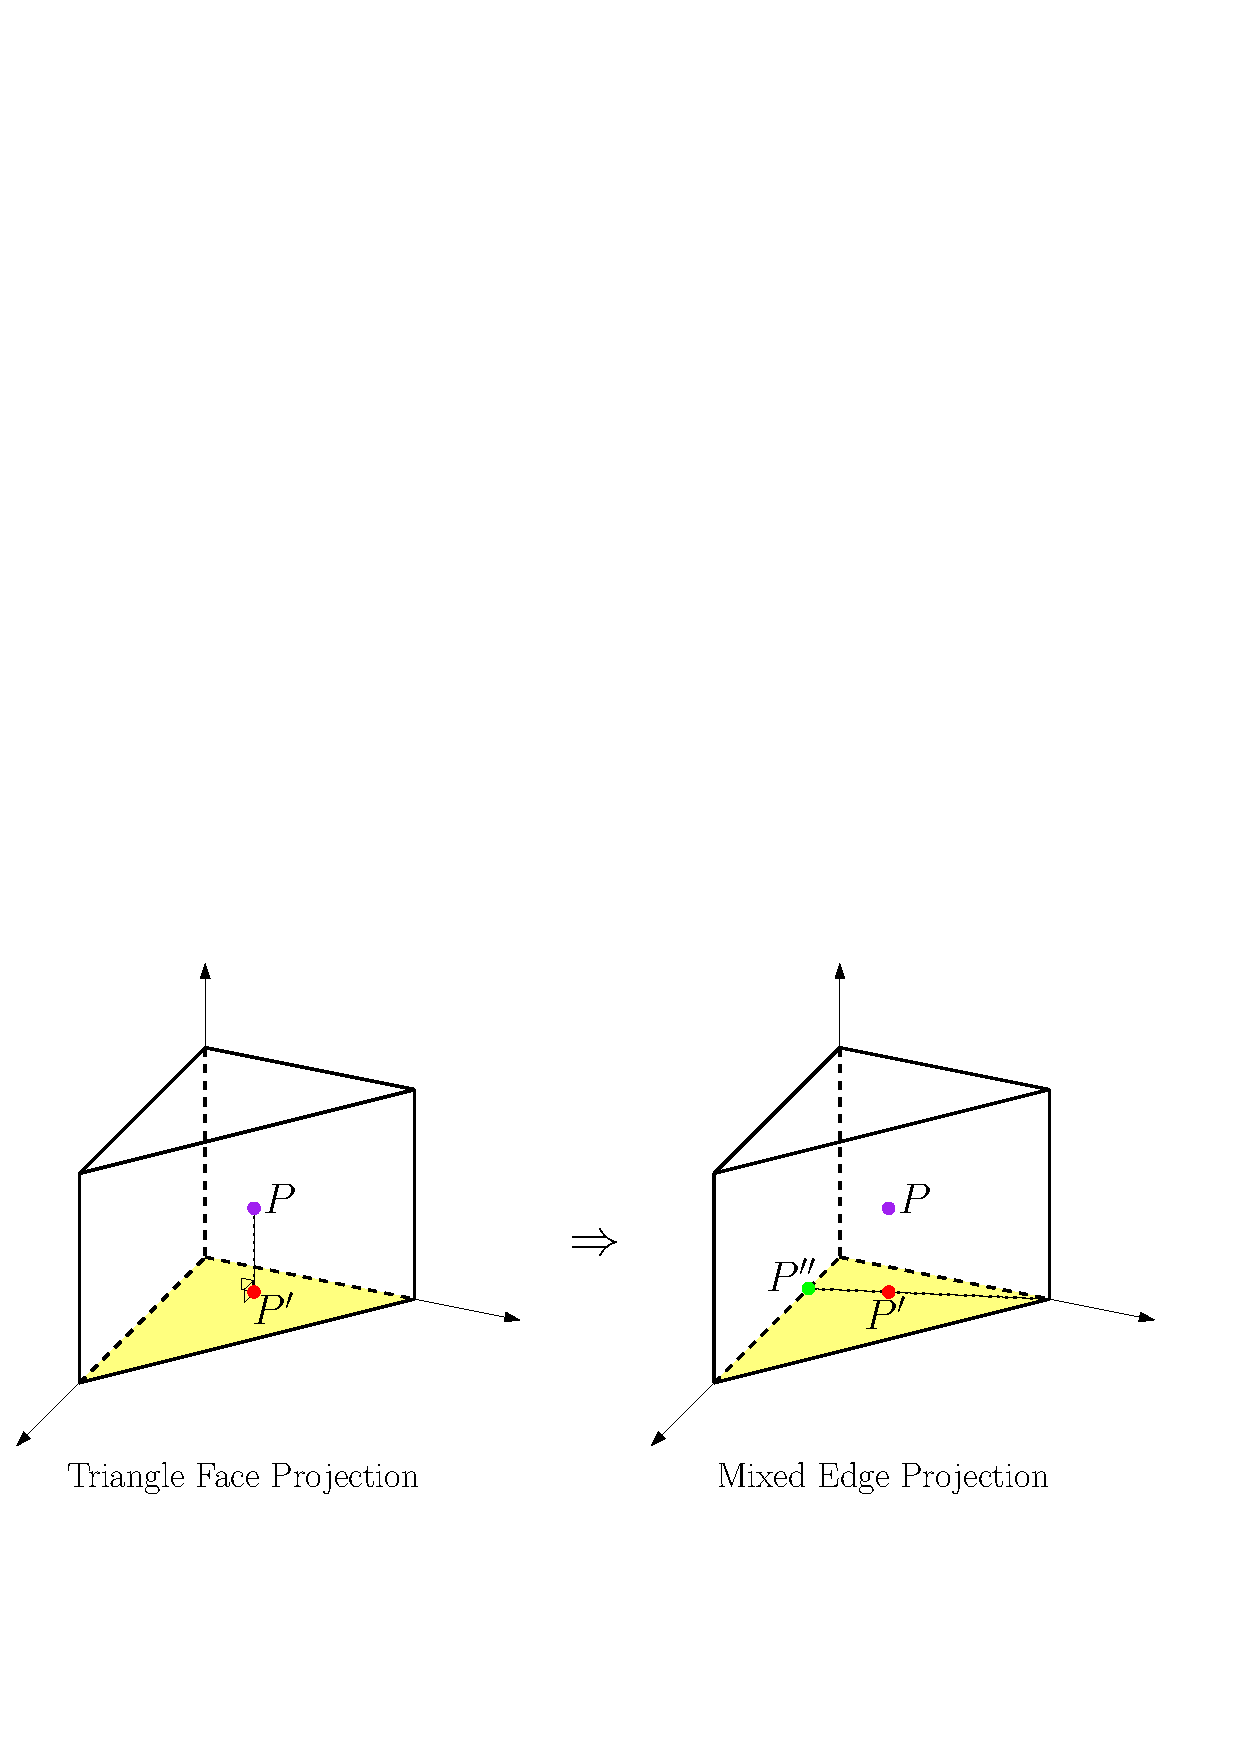
\includegraphics[scale=0.6]{./figures/PrismProjectionTriangle.pdf}
\caption{Triangle face projection from $P$ to $P'$ followed by a mixed edge projection from $P'$ to $P''$.}
\label{fig:PrismProjectionTriangle}
\end{center}
\end{figure}

%Let $\vec{\nu}_{ab}(x)=(\nu_a(x),\nu_b(x))$. 
The shape functions with their gradient are
\begin{equation}
	\begin{aligned}	
		\phi_i^\mathrm{e}(x,z)&=\mu_c(z)\phi_i^\E(\vec{\nu}_{ab}(x))\,,\\
		\nabla\phi_i^\mathrm{e}(x,z)&=\mu_c(z)\nabla\phi_i^\E(\vec{\nu}_{ab}(x))+\phi_i^\E(\vec{\nu}_{ab}(x))\nabla\mu_c(z)\,,
	\end{aligned}\label{eq:PrismH1mixededges}
\end{equation}
where $i=2,\ldots,p$, $0\leq a<b\leq2$, and $c=0,1$. 
There are $p-1$ shape functions for each mixed edge, for a total of $6(p-1)$ mixed edge functions.

%At the edge itself, $\mu_c=1$ and $\vec{\nu}_{ab}(x)$ takes the form $\vec{\mu}_{01}(x_d)$ for some $d=1,2$, so the shape function takes desired $H^1$ edge standard form, $\phi_i^\E(\vec{\mu}_{01}(x_d))$.
%As expected, there is a linear edge blending towards the adjacent quadrilateral face, given by $\mu_c(z)$, and the known triangle edge blending towards the adjacent triangle face, naturally included within $\phi_i^\E$.
%The vanishing trace properties are inherited and easily seen to be satisfied. 


%We consider first the case of the bottom horizontal edges (corresponding to $ \mu_0=1$) with orientation $\mathrm{o}=0$. Recall the triangle edge bubbles (for the $0-1$ edge of the triangle) are given as $\phi^{\mathrm{E}}_{i}(\nu_0(x,y),\nu_1(x,y))$ with $i=2,\cdots,p$ and $p$ being the edge order. The (bottom) horizontal edge shape function for the prism in this case is: \begin{equation}\phi^{e}_i(x,y,z)=\phi^{\mathrm{E}}_{i}(\nu_0(x,y),\nu_1(x,y))\mu_0(z). \nonumber \end{equation}The full set of all prismatic edge shape functions are given as \begin{equation}\phi_i^{\mathrm{E}}(\nu_a,\nu_b)\mu_{c}(z)\nonumber\end{equation} with $a<b \in \{0,1,2\}$ and where $c=1$ corresponds to the top edges and $c=0$ to the bottom edges and $i=2\ldots,p$.

%By the very construction, we see that these edge shape functions vanish at the approprite edges, i.e., for appropriate $a,b$, we see that the product $\phi_i^{\mathrm{E}}(\nu_a,\nu_b)\mu_{m}(z)$ vanishes on all edges except on edge $a-b$.
%\paragraph{Orientation Considerations}
%As before, taking into account orientations, we denote by $\phi_i^{\mathrm{E},\mathrm{o}}(\cdot)$ to indicate that the triangle edges have orientation $\mathrm{o}$. For instance, for the bottom triangle face, we have, \begin{equation}
% \phi_i^{\mathrm{E},\mathrm{o}}(\nu_0,\nu_1)\mu_{0}(z) = \phi_i^{\mathrm{E},\mathrm{o}}(\nu_1,\nu_0)\mu_{0}(z),\end{equation}
% where $\phi_i^{\mathrm{E},\mathrm{o}}(\nu_1,\nu_0)$ is the oriented $0-1$ triangle edge shape function.

\paragraph{\texorpdfstring{$H^1$}{H1} Quadrilateral Edges.}
These are the tensor product of $H^1$ triangle vertex shape functions with the 1D $H^1$ edge functions. 
For edge 03, the shape functions are
\begin{equation*}
	\phi_i^\mathrm{e}(x,z)=\underbrace{\nu_0(x)}_{\text{blend}}
		\underbrace{\phi_i^\E(\underbrace{\mu_0(z),\mu_1(z)}_{\text{project}})}_{\text{evaluate}}\,,
			%=\nu_0(x)[L_i](\mu_0(z),\mu_1(z))=\nu_0(x)L_i(z)\,.
\end{equation*}
for $i=2,\ldots,p$.
As expected, there is a linear edge blending towards both of the adjacent quadrilateral faces, given by $\nu_0(x)$, while all other trace properties are also inherited.
%In this case the projected 1D affine coordinates are simply $(\mu_0(z),\mu_1(z))$ and the projection is
The implied projection is simply
\begin{equation*}
	(x_1,x_2,z)\;\longmapsto\;(\textstyle{\frac{x_1}{1-x_2}},0,z)\;\longmapsto\;(0,0,z)\,.
\end{equation*}
It consists of finding the intersection $P'''=(0,0,z)$ of the edge with the normal plane passing through the original point $P=(x_1,x_2,x_3)$. 
Alternaltively it can be interpreted as a two step projection.
This is illustrated in Figure \ref{fig:PrismProjectionQuad}.

\begin{figure}[!ht]
\begin{center}
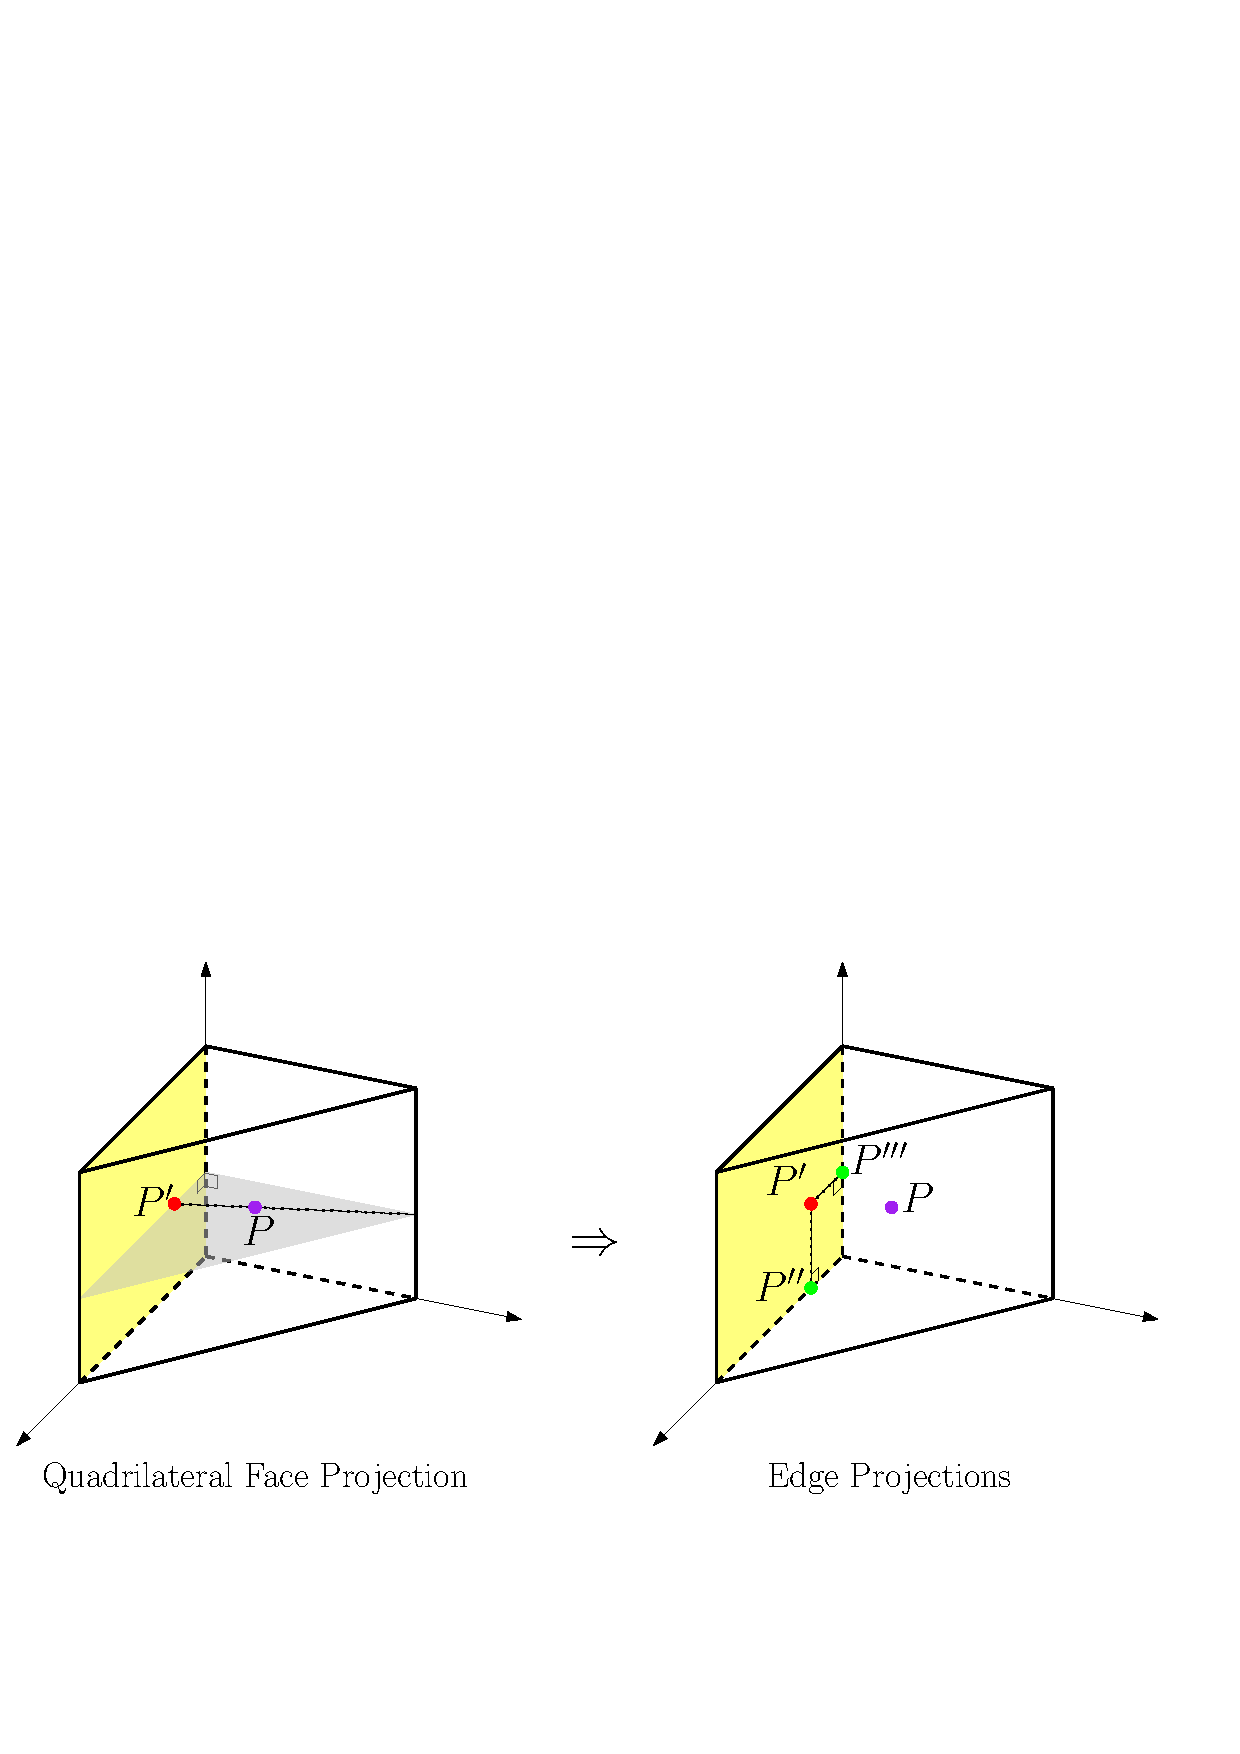
\includegraphics[scale=0.6]{./figures/PrismProjectionQuad.pdf}
\caption{Quadrilateral face projection from $P$ to $P'$ followed by a mixed edge projection from $P'$ to $P''$ and a quadrilateral edge projection from $P'$ to $P'''$.}
\label{fig:PrismProjectionQuad}
\end{center}
\end{figure}

%With $\vec{\mu}_{01}(z)=(\mu_0(z),\mu_1(z))$, the shape functions with their gradients are
The shape functions and their gradient are
\begin{equation}
	\begin{aligned}	
		\phi_i^\mathrm{e}(x,z)&=\nu_a(x)\phi_i^\E(\vec{\mu}_{01}(z))\,,\\
		\nabla\phi_i^\mathrm{e}(x,z)&=\nu_a(x)\nabla\phi_i^\E(\vec{\mu}_{01}(z))+\phi_i^\E(\vec{\mu}_{01}(z))\nabla\nu_a(x)\,,
	\end{aligned}\label{eq:PrismH1quadedges}
\end{equation}
where $i=2,\ldots,q$ and $a=0,1,2$. 
There are $q-1$ shape functions for each quadrilateral edge, for a total of $3(q-1)$ quadrilateral edge functions.

%At the edge itself, where $\nu_a=1$, the shape function takes desired $H^1$ edge standard form $\phi_i^\E(\vec{\mu}_{01}(z))$.
%As expected, there is a linear edge blending towards both of the adjacent quadrilateral faces, given by $\nu_a(x)$.
%Again, the vanishing trace properties are easily inherited. 


%the case of the edge passing through vertex $0$ where the 1D bubbles are oriented with orientation $o=0$. 
%We thus have\begin{equation}\phi_{i}^{e}(x,y,z)=\phi_{i}^{\mathrm{E}}(\mu_0(z),\mu_1(z))\nu_0(x,y)\nonumber \end{equation}with $i=2,\cdots,p$.
%The complete set of all edge shape functions is \begin{equation}\phi_{i}^{e}(x,y,z)=\phi_{i}^{\mathrm{E}}(\mu_0(z),\mu_1(z))\nu_a(x,y) \end{equation}and $a=0,1,2$
%As was the case with shared edges, these also satisfy the appropriate vanishing properties by construction.
%
%\paragraph{Orientation Considerations}
%As before, taking into account orientation, consider the $0-1$ edge. The complete set of vertical edge shape functions is given as $\phi_i^{\mathrm{E},\mathrm{o}}(\mu_{0},\mu_{1})\nu_a(x,y)$, where $\phi_i^{\mathrm{E},\mathrm{o}}(\cdot)$ indicates that the 1D segment has orientation $\mathrm{o}$.

\subsubsection{\texorpdfstring{$H^1$}{H1} Faces} 
%Here again, we have two sets of face shape functions, those that correspond to the horizontal (triangle) faces and those that correspond to the vertical (rectangular) faces.

\paragraph{\texorpdfstring{$H^1$}{H1} Triangle Faces.} 
These are tensor products of $H^1$ triangle face bubbles and 1D $H^1$ vertex shape functions. 
%As before, we first consider the bottom ($\mu_0=1$) triangle face with orientation $\mathrm{o}=0$. 
%To begin, first consider face 012 as an example. The shape functions would be of the form
For instance, for face 012 the shape functions are
\begin{equation*}
	\phi_{ij}^\mathrm{f}(x,z)=\underbrace{\mu_0(z)}_{\text{blend}}
		\underbrace{\phi_{ij}^\Tri(\underbrace{\nu_0(x),\nu_1(x),\nu_2(x)}_{\text{project}})}_{\text{evaluate}}\,,
\end{equation*}
for $i\geq2$ and $j\geq1$.
The trace properties are trivially inherited from each of the components.
The triangle face projection is illustrated in Figure \ref{fig:PrismProjectionTriangle} and consists of finding the intersection $P'=(x_1,x_2,0)$ of the face with the normal line passing through the original point $P=(x_1,x_2,x_3)$.
%The projected 2D affine coordinates are simply $(\nu_0,\nu_1,\nu_2)$, so that the projection is
%\begin{equation*}
%	(x_1,x_2,z)\;\longmapsto\;(x_1,x_2,0)\,.
%\end{equation*}
%This is obtained by finding the intersection $P'=(x_1,x_2,0)$ of the face with the normal line passing through the original point $P=(x_1,x_2,x_3)$. It is shown in Figure \textit{add Figure}.

%Given the triangle face function $\phi_{ij}^{\Tri}(\nu_0(x,y),\nu_1(x,y),\nu_2(x,y))$, with $i \geq 2, j \geq 1, i+j=2, \ldots, p$ and the 1D vertex shape function $\mu_1(z)$ we see that the (bottom) horizontal face shape function of the prism is\begin{equation}\phi_{ij}^f(x,y,z) = \phi_{ij}^{\Tri}(\nu_0(x,y),\nu_1(x,y),\nu_2(x,y))\mu_1(z).\end{equation}
%Note that since these are essentially triangle bubbles tensored with 1D vertex functions, they vanish on the boundary of the triangle faces by construction.
%Let $\vec{\nu}_{012}(x)=(\nu_0(x),\nu_1(x),\nu_2(x))$. 
In general, the shape functions and their gradient are
\begin{equation}
	\begin{aligned}	
		\phi_{ij}^\mathrm{f}(x,z)&=\mu_c(z)\phi_{ij}^\Tri(\vec{\nu}_{012}(x))\,,\\
		\nabla\phi_{ij}^\mathrm{f}(x,z)&=\mu_c(z)\nabla\phi_{ij}^\Tri(\vec{\nu}_{012}(x))
			+\phi_{ij}^\Tri(\vec{\nu}_{012}(x))\nabla\mu_c(z)\,,
	\end{aligned}\label{eq:PrismH1TriFace}
\end{equation}
where $i\geq2$, $j\geq1$, $n=i+j=3,\ldots,p$, and $c=0,1$. 
As with any $H^1$ triangle face, there are $\frac{1}{2}(p-1)(p-2)$ shape functions per face, for a total of $(p-1)(p-2)$ triangle face  functions.

%The shape functions are compatible with neighboring triangle faces, since at the face, where $\mu_c=1$, they are of the form $\phi_{ij}^\Tri(\nu_0(x),\nu_1(x),\nu_2(x))$, which is the $H^1$ standard form for triangle faces. The other vanishing properties are naturally inherited from $\mu_c$ and $\phi_{ij}^\Tri$.

%\paragraph{Orientation Considerations}
%Taking into account orientation, the complete set of horizontal face shape functions is given by $\phi_{ij}^{\Tri,\mathrm{o}}(\nu_0,\nu_1,\nu_2)\mu_c(z)$, $c=0,1$ and $\phi_{ij}^{\mathrm{\Tri},\mathrm{o}}(\cdot)$ refers to the triangle face shape function with orientation $\mathrm{o}$. Note that, as given in the triangle section, we permute the arguments $\nu_0,\nu_1,\nu_2$ of $\phi_{ij}^{\Tri}(\cdot,\cdot,\cdot)$ with the $6$ possible permutations of the axes to arrive at the complete set of shape functions.

\paragraph{\texorpdfstring{$H^1$}{H1} Quadrilateral Faces.} 
%The construction of the vertical face shape functions is a bit more involved. We first consider the case of unswapped axes. We have\begin{equation}\phi_{ij}^f(x,y,z) = \phi_{ij}^{\square}(\nu_a,\nu_b,\mu_0,\mu_1),\end{equation}where $a<b \in \{0,1,2\},$ with $i=2,\ldots,p, j=2,\ldots,q.$ The face function $\phi_{ij}^{\square}(\nu_a,\nu_b,\mu_0,\mu_1)$ is as given in the quadrilateral section. Note here that the polynomial order is $p$ for the triangle edge bubbles and $q$ for the 1D bubbles.
The quadrilateral face functions are simply the product $H^1$ triangle edge functions and 1D $H^1$ edge functions, so they conveniently fall into the general definition of $\phi_{ij}^\square$.
For face 0143, they take the form
\begin{equation*}
	\phi_{ij}^\mathrm{f}(x,z)=\phi_{ij}^\square(\vec{\nu}_{01}(x),\vec{\mu}_{01}(z))
		=\underbrace{(\nu_0(x)+\nu_1(x))^i}_{\text{blend}}
			\underbrace{\phi_{ij}^\square\Big(\underbrace{\textstyle{\frac{1}{\nu_0(x)+\nu_1(x)}}
				\vec{\nu}_{01}(x),\vec{\mu}_{01}(z)}_{\text{project}}\Big)}_{\text{evaluate}}\,,
\end{equation*}
where $i=2,\ldots,p$ and $j=2,\ldots,q$.
Clearly, the desired trace properties are inherited.
%Here, there are two pairs of 1D projected affine coordinates. 
%The first one is $(\frac{\nu_0}{\nu_0+\nu_1},\frac{\nu_1}{\nu_0+\nu_1})$, while the second one is simply $(\mu_0(z),\mu_1(z))$. 
%They represent a projection of the form
%\begin{equation*}
%	(x_1,x_2,z)\;\longmapsto\;(\textstyle{\frac{x_1}{1-x_2}},0,z)\,.
%\end{equation*}
The implied projection, already illustrated in Figure \ref{fig:PrismProjectionQuad}, consists of finding the intersection $P'=(\frac{x_1}{1-x_2},0,z)$ of the face with the projecting line lying in the horizontal plane and passing through the original point $P=(x_1,x_2,x_3)$ and the opposite disjoint quadrilateral edge. 

%Let $\vec{\nu}_{ab}(x)=(\nu_a(x),\nu_b(x))$ and $\vec{\mu}_{01}(z)=(\mu_0(z),\mu_1(z))$. 
The shape functions and their gradient are
\begin{equation}
%	\begin{aligned}	
		\phi_{ij}^\mathrm{f}(x,z)=\phi_{ij}^\square(\vec{\nu}_{ab}(x),\vec{\mu}_{01}(z))\,,\qquad\quad
		\nabla\phi_{ij}^\mathrm{f}(x,z)=\nabla\phi_{ij}^\square(\vec{\nu}_{ab}(x),\vec{\mu}_{01}(z))\,,
%	\end{aligned}\label{eq:PrismH1QuadFace}
\end{equation}
where $i=2,\ldots,p$, $j=2,\ldots,q$, and $0\leq a<b\leq2$. 
There are $(p-1)(q-1)$ shape functions per face, leading to a total of $3(p-1)(q-1)$ quadrilateral face functions.

%The shape functions are compatible with neighboring quadrilateral faces. To see this, note that at the quadrilateral face, $\vec{\nu}_{ab}(x)$ takes the form $\vec{\mu}_{01}(x_d)$ for some $d=1,2$. 
%Hence, the shape functions take the $H^1$ standard form for quadrilateral faces, $\phi_{ij}^\square(\vec{\mu}_{01}(x_d),\vec{\mu}_{01}(z))$. 
%Meanwhile, the other vanishing properties are easily seen to be satisfied.

%Again, these vanish on the quadrilateral edges by construction and also on the shared edges due to the vanishing of the 1D bubbles on the shared triangle edge. Thus, the quadrilateral face functions also satisfy the vanishing properties as required.
%\paragraph{Orientation Considerations}
%We now come to the case of swapped axes. In the case of swapped coordinates, the ordering of the edge functions changes.
%Recall the orientation consideration presented earlier in the case of rectangular faces. The case of swapped axes corrsepond to the case $\mathrm{o}=1$. We then have the complete list of face shap functions, given by: \begin{equation}\phi_{ij}^f(x,y,z) = \phi_{ij}^{\square}(\nu_a,\nu_b,\mu_0,\mu_1) = \phi_{i}^{\mathrm{E},\mathrm{o}}(\nu_a,\nu_b)\phi_{j}^{\mathrm{E},\mathrm{o}}(\mu_0,\mu_1),\end{equation}where , $\phi^{\mathrm{E},\mathrm{o}}(\cdot)$ indicates edge shape functions with orientation $\mathrm{o}$ of the triangle element and segment element with the obvious changes in argument.

\subsubsection{\texorpdfstring{$H^1$}{H1} Interior Bubbles} 
The $H^1$ bubble functions are the tensor product of the $H^1$ triangle face functions and 1D $H^1$ edge functions.
Due to their structure, the zero trace properties are trivially satisfied along the whole boundary.
%With $\vec{\nu}_{012}(x)=(\nu_0(x),\nu_1(x),\nu_2(x))$ and $\vec{\mu}_{01}(z)=(\mu_0(z),\mu_1(z))$, they are

The interior bubbles and their gradient are
\begin{equation}
	\begin{aligned}	
		\phi_{ijk}^\mathrm{b}(x,z)&=\phi_{ij}^\Tri(\vec{\nu}_{012}(x))\phi_k^\E(\vec{\mu}_{01}(z))\,,\\
		\nabla\phi_{ijk}^\mathrm{b}(x,z)&=\phi_k^\E(\vec{\mu}_{01}(z))\nabla\phi_{ij}^\Tri(\vec{\nu}_{012}(x))
			+\phi_{ij}^\Tri(\vec{\nu}_{012}(x))\nabla\phi_k^\E(\vec{\mu}_{01}(z))\,,
	\end{aligned}
\end{equation}
where $i\geq2$, $j\geq1$, $n=i+j=3,\ldots,p$, and $k=2,\ldots,q$. 
There are a total of $\frac{1}{2}(p-1)(p-2)(q-1)$ bubble shape functions in $H^1$.

%The vanishing properties are trivially inherited and checked to hold.

%Given the triangle bubble function $\phi_{ij}^{\Tri}(\nu_0,\nu_1,\nu_2) $ and the 1D bubble function $\phi^{\mathrm{E}}_{k}(\mu_{0}(z),\mu_1(z))$ we have \begin{equation}\phi^{b}_{ijk}(x,y,z) = \phi_{ij}^{\Tri}(\nu_0,\nu_1,\nu_2)\phi_k^{\mathrm{E}}(\mu_0,\mu_1).\end{equation}Here, $i\geq2, j\geq1, i+j=2,\ldots,p$ and $k=2,\dots,q$, where $p$ and $q$ are the polynomial order for the triangle face bubble and 1D bubble respectively. Also, we do not worry about the orientation, as the interior bubble functions are not oriented. By the very construction, the bubble functions are nonzero only on the interior of the prism.



\subsection{\texorpdfstring{$H(\mathrm{curl})$}{Hcurl} Shape Functions}

The linearly independent shape functions presented here are shown to belong and span the $H(\mathrm{curl})$ conforming space $(\mathcal{N}^p\otimes\mathcal{P}^q)\times(\mathcal{P}^p\otimes\mathcal{P}^{q-1})$, which has dimension $p(p+2)(q+1)+\frac{1}{2}(p+2)(p+1)q$.

%%We begin our discussion of $H(\text{curl})$ shape functions with {$H(\text{curl})$} edge functions.
%The $H(\mathrm{curl})$ conforming finite dimensional space is 
%%The dimension of this space is $p(p+2)(q+1)+\frac{1}{2}(p+2)(p+1)q$.
%The shape functions presented here are shown to lie in that space, and by linear independence, they span the space.
%%To see that the shape functions lie in this space, they will be shown in more explicit form, from which it will

These shape functions, as expected, are composed of combinations of $H^1$ and $H(\mathrm{curl})$ components. 
Intuitively, they involve the affine coordinates and at least $E_i^\E$, $E_{ij}^\Tri$ and $E_{ij}^\square$.
All shape functions continue to respect the logic of projecting, evaluating and blending, and for a given topological entity, the projections are the same as those in $H^1$ (see Figures \ref{fig:PrismProjectionTriangle} and \ref{fig:PrismProjectionQuad}).

%It will be clear that all shape functions lie in $\mathcal{P}^p\otimes\mathcal{P}^q$, which has dimension $\frac{1}{2}(p+2)(p+1)(q+1)$. 
%Moreover, a judicious count of the shape functions constructed in this section will coincide with that dimension, ensuring that the span of these is precisely $\mathcal{P}^{p}\otimes\mathcal{P}^q$.


\subsubsection{\texorpdfstring{$H(\mathrm{curl})$}{Hcurl} Edges}
%As was the case with {$H^1$} edge functions, we consider two cases, the horizontal and vertical edge functions.

\paragraph{\texorpdfstring{$H(\mathrm{curl})$}{Hcurl} Mixed Edges.} 
These are tensor products of triangle $H(\text{curl})$ edge functions and 1D $H^1$ vertex functions.
For example, take edge 01. 
Note that $E_i^\E(\vec{\nu}_{01}(x))$ in three dimensions is a three component vector whose last component is zero, since it is independent of the $z$ coordinate. 
Indeed, if considered in \textit{two} dimensions, it is just the well defined triangle $H(\text{curl})$ edge function. 
As such, it is an element of $\mathcal{N}^p$ (in two dimensions). 
Due to this important fact, the first two components of $E_i^\E$ are denoted by $(E_i^\E(\vec{\nu}_{01}(x)))_x\in\mathcal{N}^p$. 
For this edge, the shape functions are
\begin{equation*}
	\begin{aligned}
		E_i^\mathrm{e}(x,z)&=\mu_0(z)E_i^\E(\vec{\nu}_{01}(x))
			%=\begin{pmatrix}\mu_0(z)(E_i^\E(\vec{\nu}_{01}(x)))_{x_1}\\\mu_0(z)(E_i^\E(\vec{\nu}_{01}(x)))_{x_2}\\0\end{pmatrix}
				=\begin{pmatrix}\mu_0(z)(E_i^\E(\vec{\nu}_{01}(x)))_x\\0\end{pmatrix}
					\in(\mathcal{N}^p\otimes\mathcal{P}^1)\times\{0\}\\
		  &=\underbrace{\mu_0(z)(\nu_0(x)+\nu_1(x))^{i+2}}_{\text{blend}}
    		\underbrace{E_i^\E\Big(\underbrace{\textstyle{\frac{1}{\nu_0(x)+\nu_1(x)}\vec{\nu}_{01}(x)}}_{\text{project}}
    			\Big)}_{\text{evaluate}}\,,
	\end{aligned}
\end{equation*}
for $i=0,\ldots,p-1$.
Hence, $E_i^\mathrm{e}\in(\mathcal{N}^p\otimes\mathcal{P}^q)\times(\mathcal{P}^p\otimes\mathcal{P}^{q-1})$.
For the trace properties, note that over faces 1254 and 0253 both tangential components are zero, since the $z$ component is zero and the tangent to edges 12 and 02 is zero by inheritance of $E_i^\E(\vec{\nu}_{01}(x))$.
In the top face, the tangent is also zero because $\mu_0(z)$ is zero there.
Finally, by construction, over face 012 its tangent is precisely the triangle $H(\text{curl})$ edge shape function $(E_i^\E(\vec{\nu}_{01}(x)))_x$, while over face 0143 its tangent behaves like a quadrilateral $H(\text{curl})$ edge function $\mu_0(z)(E_i^\E(\vec{\mu}_{01}(x_1)))_x$.
%The same will apply to the other mixed edges. 
%As an observation, note the curl of the expression above can be expressed in terms of the two dimensional curl and the one dimensional gradient. For this, denote by $\nabla_x\times(E_i^\E(\nu_0(x),\nu_1(x)))_x$ the 2D curl, and by $\nabla_z\mu_0(z)$ the one dimensional gradient. Then,
%\begin{equation*}
%	\nabla\times E_i^\mathrm{e}=\begin{pmatrix}-\nabla_z\mu_0(E_i^\E(\nu_0,\nu_1))_{x_2}\\\nabla_z\mu_0(E_i^\E(\nu_0,\nu_1))_{x_1}\\
%			\mu_0\nabla_x\times(E_i^\E(\nu_0,\nu_1))_x\end{pmatrix}\,.
%\end{equation*}

Now, the general shape functions and their curl are
\begin{equation}
	\begin{aligned}	
		E_i^\mathrm{e}(x,z)&=\mu_c(z)E_i^\E(\vec{\nu}_{ab}(x))\,,\\
		\nabla\times E_i^\mathrm{e}(x,z)&=\mu_c(z)\nabla\times E_i^\E(\vec{\nu}_{ab}(x))
			+\nabla\mu_c(z)\times E_i^\E(\vec{\nu}_{ab}(x))\,,
	\end{aligned}
\end{equation}
with $i=0,\ldots,p-1$, $0\leq a<b\leq2$ and $c=0,1$. 
There are $p$ shape functions for each mixed edge, giving a total of $6p$ mixed edge functions.

%At the edge itself, $\mu_c=1$ and $\vec{\nu}_{ab}(x)$ takes the form $\vec{\mu}_{01}(x_d)$ for some $d=1,2$, so the shape function takes the form $E_i^\E(\vec{\mu}_{01}(x_d))$, whose (tangential) trace is the $L^2$ edge standard form $[P_i](\vec{\mu}_{01}(x_d))$.
%As before, there is a linear edge blending towards the adjacent quadrilateral face, given by $\mu_c(z)$, and the known triangle edge blending towards the adjacent triangle face, naturally included within $E_i^\E$. 
%The remaining vanishing trace properties are easily seen to be inherited.

%Recall the $H(\text{curl})$ edge shape functions for the triangle (with edge ($\nu_{0},\nu_{2}) $) are given as $E_i^{e}(x,y)=E_{i}^{\mathrm{E}}(\nu_{0},\nu_{2}), i\leq p-1$ (assuming orientation $\mathrm{o}=0$). Since $E^e_{i}(x,y)$ is a vector field, it will be convenient to write it in coordinates where $E^\mathrm{E}_{i,1}(\cdot)$ and $E^\mathrm{E}_{i,2}(\cdot)$ are the components of $E^e_{i}(\cdot)$. The horizontal $H(\text{curl})$ edge shape functions are given as:

%\begin{equation} E_{i}^{e}(x,y,z) = \left(
%\begin{array}{c}
%E_{i,1}^{\mathrm{E}}(\nu_{0},\nu_{1})\,\mu_{0}(z)\\
%\\
%E_{i,2}^{\mathrm{E}}(\nu_{0},\nu_{1})\,\mu_{0}(z)\\
%\\
%0 \\
%\end{array}
%\right),
%\nonumber
%\end{equation}
%\\
%\begin{equation} \nabla\times E_{i}^{e}(x,y,z) = \left(
%\begin{array}{c}
%-E_{i,2}^{\mathrm{E}}(\nu_{0},\nu_{1})\,(\nabla \mu_{0}(z))_{,3}\\
%\\
%E_{i,1}^{\mathrm{E}}(\nu_{0},\nu_{1})\,(\nabla \mu_{0}(z))_{,3}\\
%\\
%\nabla \times (E_{i,1}^{\mathrm{E}},E_{i,2}^{\mathrm{E}})\,\mu_{0}(z) \\
%\end{array}
%\right),
%\nonumber
%\end{equation}
%where the $\nabla \times$ is interpreted in 3D and $(\nabla \mu_{0}(z))_{,3}$ denotes the third component of the gradient computed in 3D.
%We can write the above equations compactly by noting \begin{equation}E_{i}^{e}(x,y,z) = E_{i}^{\mathrm{E}}(\nu_{0},\nu_{1})\mu_{0}(z)\nonumber \end{equation} where we interpret $E_{i}^{\mathrm{E}}(\nu_{0},\nu_{1})$ and $\mu_{0}(z)$ as appropriate 3D vectors, so that we have
%\begin{equation}
%\nabla\times E_{i}^{e}(x,y,z)=\mu_0(z)\nabla \times(E_{i}^{\mathrm{E}}(\nu_{0},\nu_{1}))+ \nabla \mu_0(z)\times E_{i}^{\mathrm{E}}(\nu_{0},\nu_{1}),
%\nonumber \end{equation}
%where we interpret $\nabla \times (E_{i}^{\mathrm{E}}(\nu_{0},\nu_{1}))$ as $(\nabla \times(E_{i,1}^{\mathrm{E}}(\cdot),E_{i,2}^{\mathrm{E}}(\cdot)),0) $ the gradient $\nabla\mu_{0}(z)$ as the vector $(0,0,\mu^\prime_{0}(z))$. Again, the functions satisfy the vanishing properties by construction, i.e., the edge function corresponding to edge $0-1$ vanishes on all edges except edge $0-1$. The complete family of (unoriented) $H(\text{curl})$ mixed edge shape functions is given as \begin{equation} E_{i}^{e}(x,y,z) = E_{i}^{\mathrm{E}}(\nu_{a},\nu_{b})\mu_{c}(z)
%\end{equation}
%and 
%\begin{equation}
%\nabla\times E_{i}^{e}(x,y,z)=\mu_c(z)\nabla \times (E_{i}^{\mathrm{E}}(\nu_{a},\nu_{b}))+ \nabla \mu_c(z)\times E_{i}^{\mathrm{E}}(\nu_{a},\nu_{b}),
%\end{equation}
%where $0 \leq a \leq b \leq 2$ and $c=0,1$.
%\paragraph{Orientation Considerations}
%As we saw earlier, to incorporate orientations to the $0-1$ edge of the bottom face, we modify the above equations as \begin{equation}E_{i}^{e}(x,y,z) = E_{i}^{\mathrm{E},\mathrm{o}}(\nu_{0},\nu_{1})\mu_{0}(z).\end{equation}
%The orientation of other faces similarly follows. 

\paragraph{\texorpdfstring{$H(\mathrm{curl})$}{Hcurl} Quadrilateral Edges.} 
%These are tensor products of triangle $H^{1}$ vertex shape functions and 1D $L^2$ shape functions. Considering again the orientation $\mathrm{o}=0$ case of the quadrilateral edge passing through vertex $0$, we have, in coordinates:
These are tensor products of triangle $H^1$ vertex shape functions and $E_i^\E(\vec{\mu}_{01}(z))$, which act as 1D $H(\mathrm{curl})$ functions (even though these do not formally exist for the segment element).
For instance, take edge 03. 
Now, $E_i^\E(\vec{\mu}_{01}(z))$ in three dimensions is a three component vector whose first two components are zero, since it is only dependent on the $z$ coordinate. 
Indeed, if considered in \textit{one} dimension, it is just a segment $L^2$ function belonging to $\mathcal{P}^{q-1}$. 
This last component of $E_i^\E$ is denoted by $(E_i^\E(\vec{\mu}_{01}(z)))_z\in\mathcal{P}^{q-1}$. 
For this edge, the shape functions are
\begin{equation*}
	E_i^\mathrm{e}(x,z)=\underbrace{\nu_0(x)}_{\text{blend}}
			\underbrace{E_i^\E(\underbrace{\vec{\mu}_{01}(z)}_{\text{project}})}_{\text{evaluate}}
		=\begin{pmatrix}0\\0\\\nu_0(x)(E_i^\E(\vec{\mu}_{01}(z)))_{z}\end{pmatrix}
			\in\{0\}\times\{0\}\times(\mathcal{P}^1\otimes\mathcal{P}^{q-1})\,,
\end{equation*}
for $i=0,\ldots,q-1$.
Clearly $E_i^\mathrm{e}\in(\mathcal{N}^p\otimes\mathcal{P}^q)\times(\mathcal{P}^p\otimes\mathcal{P}^{q-1})$.
The trace properties follow easily for the triangle faces, since the vector field points normal to those faces, while in the nonadjacent quadrilateral face 1254 it is zero due to $\nu_0(x)$ being zero.
In the adjacent faces, $E_i^\E(\vec{\mu}_{01}(z))$ is unaffected by the restictions (it is already tangent to the faces and independent of $x$), so the tangential trace is a quadrilateral $H(\text{curl})$ edge function simply because the restriction of $\nu_0(x)$ is a linear blending function over that face.

In view of \eqref{eq:Hcurl1Dspecialcase}, the shape functions and their curl are
\begin{equation}
%	\begin{aligned}	
		E_i^\mathrm{e}(x,z)=\nu_a(x)E_i^\E(\vec{\mu}_{01}(z))\,,\qquad\quad
		\nabla\times E_i^\mathrm{e}(x,z)=\nabla\nu_a(x)\times E_i^\E(\vec{\mu}_{01}(z))\,,
%	\end{aligned}
\end{equation}
with $i=0,\ldots,q-1$, and $a=0,1,2$. 
There are $q$ shape functions for each quadrilateral edge, for a total of $3q$ quadrilateral edge functions.

%%%%At the edge itself, where $\nu_a=1$, the shape function takes desired $H(\mathrm{curl})$ edge standard form $E_i^\E(\vec{\mu}_{01}(z))$.
%%%%As expected, there is a linear edge blending towards both of the adjacent quadrilateral faces, given by $\nu_a(x)$.
%%%%Again, the vanishing trace properties are easily inherited. 

%\begin{equation} E_{i}^e(x,y,z) = \left(
%\begin{array}{c}
%0\\
%\\
%0\\
%\\
%\nu_0(x,y)\,E_{i,3}^{\mathrm{E}}(\mu_0,\mu_1) \\
%\end{array}
%\right),
%\nonumber
%\end{equation}
%\\
%\begin{equation} \nabla\times E_{i}^{e}(x,y,z) = \left(
%\begin{array}{c}
%\frac {\partial\nu_0(x,y)}{\partial y}\,E_{i,3}^{\mathrm{E}}(\mu_0,\mu_1)\\
%\\
%-\frac {\partial\nu_0(x,y)}{\partial x}\,E_{i,3}^{\mathrm{E}}(\mu_0,\mu_1)\\
%\\
%0 \\
%\end{array}
%\right),
%\nonumber
%\end{equation}
%so that we have
%\begin{equation}
% E_{i}^e(x,y,z) = \nu_0(x,y) E_i^{\mathrm{E}}(\mu_0,\mu_1)
%\nonumber
%\end{equation}
%and
%\begin{equation}
%\nabla\times E_{i}^{e}(x,y,z)=\nabla\nu_0(x,y)\times E_i^{\mathrm{E}}(\mu_0,\mu_1),
%\nonumber
%\end{equation}
%where $i=1,\ldots, p$. Again, we interpret the compact equations appropriately in 3D.
%In the above equation, $\nu_0(x,y)$ is the triangle vertex function corresponding to vertex $0$ and we interpret $\nabla\nu_0(x,y)$ as the three-dimensional gradient. Also, $E_i^{\mathrm{E}}(\mu_0,\mu_1)$ is the $i$-th 1D $L^2$ shape function, $i=1,\cdots,p$. Moreover, the functions satisfy the vanishing properties by construction, i.e., the edge function corresponding to vertex $0$ vanishes on all other edges. For the complete list of all $H(\text{curl})$ quadrilateral edge shape functions, we have  \begin{equation} E_{i}^e(x,y,z) = \nu_a(x,y) E_i^{\mathrm{E}}(\mu_0,\mu_1)
%\end{equation}
%and 
%\begin{equation}
%\nabla\times E_{i}^{e}(x,y,z)=(\nabla\nu_a(x,y)\times E_i^{\mathrm{E}}(\mu_0,\mu_1),
%\end{equation}
%where $a=0,1,2$.
%\paragraph{Orientation Considerations}
%As is usual, after incorporating orientations, the modified equations (for the edge passing through vertext $0$) are:\begin{equation} E_{i}^e(x,y,z) = \nu_a(x,y) E_{i}^{\mathrm{E},\mathrm{o}}(x,y,z)
%\end{equation}

\subsubsection{\texorpdfstring{$H(\mathrm{curl})$}{Hcurl} Faces}
%We now consider {$H(\text{curl})$} face shape functions. As was the case with {$H^1$} face functions, we consider two cases, the horizontal (triangle) and vertical(rectangular) face functions.

\paragraph{\texorpdfstring{$H(\mathrm{curl})$}{Hcurl} Triangle Faces.} 
These are tensor products of triangle $H(\text{curl})$ face functions and $H^1$ vertex shape functions. 
As usual, there are two families. 
Proceeding as with $H(\text{curl})$ mixed edge functions, it follows the shape functions lie in $(\mathcal{N}^p\otimes\mathcal{P}^q)\times(\mathcal{P}^p\otimes\mathcal{P}^{q-1})$ and that the trace properties are satisfied.
%They will also be naturally compatible at the faces themselves, and vanish at the other faces. 
As accustomed, there are $p(p-1)$ functions per triangle face, and a grand total of $2p(p-1)$ triangle face functions.

\subparagraph{Family I:} 
The shape functions and their curl are
\begin{equation}
	\begin{aligned}
		E_{ij}^{\mathrm{f}}(x,z)&=\mu_c(z)E_{ij}^\Tri(\vec{\nu}_{012}(x))\,,\\
		\nabla\times E_{ij}^{\mathrm{f}}(x,z)&=\mu_c(z)\nabla\times E_{ij}^\Tri(\vec{\nu}_{012}(x))
			+\nabla\mu_c(z)\times E_{ij}^\Tri(\vec{\nu}_{012}(x))\,,
	\end{aligned}
\end{equation}
for $i\geq0$, $j\geq1$, $n=i+j=1,\ldots,p-1$, and $c=0,1$. 
For every face, there are $\frac{1}{2}p(p-1)$ functions in this family.

\subparagraph{Family II:}
The shape functions and their curl are
\begin{equation}
	\begin{aligned}
		E_{ij}^{\mathrm{f}}(x,z)&=\mu_c(z)E_{ij}^\Tri(\vec{\nu}_{120}(x))\,,\\
		\nabla\times E_{ij}^{\mathrm{f}}(x,z)&=\mu_c(z)\nabla\times E_{ij}^\Tri(\vec{\nu}_{120}(x))
			+\nabla\mu_c(z)\times E_{ij}^\Tri(\vec{\nu}_{120}(x))\,,
	\end{aligned}
\end{equation}
for $i\geq0$, $j\geq1$, $n=i+j=1,\ldots,p-1$, and $c=0,1$.
Note the fact that the entries are $\vec{\nu}_{120}(x)$ as opposed to $\vec{\nu}_{012}(x)$.
For every face, there are $\frac{1}{2}p(p-1)$ functions in this family.


%Recall that (one family of) the triangle $H(\text{curl})$ bubbles are given as $E_{ij}^{f}(x,y)=E_{ij}^{\Tri}(\nu_0,\nu_1,\nu_2)$ with $ i\geq0, j\geq1,i + j = 1,\cdots, p-1.$ Thus, the horizontal $H(\text{curl})$ face shape functions are (as before, in coordinates and $c=0$, i.e., the bottom triangle face)
%
%\begin{equation} E_{ij}^{f}(x,y,z) = \left(
%\begin{array}{c}
%E_{ij,1}^{\Tri}(\nu_0,\nu_1,\nu_2)\,\mu_{0}(z)\\
%\\
%E_{ij,2}^{\Tri}(\nu_0,\nu_1,\nu_2)\,\mu_{0}(z)\\
%\\
%0 \\
%\end{array}
%\right),
%\nonumber
%\end{equation}
%\\
%\begin{equation} \nabla \times E_{ij}^{f}(x,y,z) = \left(
%\begin{array}{c}
%-E_{ij,2}^{\Tri}(\nu_0,\nu_1,\nu_2)\,(\nabla \mu_0(z))_{,3}\\
%\\
%E_{ij,1}^{\Tri}(\nu_0,\nu_1,\nu_2)\,(\nabla \mu_0(z))_{,3}\\
%\\
%\nabla \times (E_{ij,1}^{\Tri},E_{ij,2}^{\Tri})\,\mu_0(z) \\
%\end{array}
%\right),
%\nonumber
%\end{equation}
%so that we have
%\begin{equation} E_{ij}^{f}(x,y,z) = E_{ij}^{\Tri}(\nu_0,\nu_1,\nu_2)\mu_{0}(z)\nonumber \end{equation}
%and 
%\begin{equation}
%\nabla \times E_{ij}^{f}(x,y,z)=\mu_0(z)\nabla \times(E_{ij}^{\Tri}(\nu_0,\nu_1,\nu_2))+\nabla\mu_0(z) \times E_{ij}^{\Tri}(\nu_0,\nu_1,\nu_2),
%\nonumber \end{equation}
%where we again interpret $\nabla \times(E_{ij}^{\Tri}(\nu_0,\nu_1,\nu_2))$ in 3D and $\nabla\mu_0(z)$ as $(0,0,\mu^\prime_0(z)) $. Also, the functions satisfy the vanishing properties by construction, i.e., the face function corresponding to the bottom triangle face vanishes on the entire boundary of the triangle. The complete set of $H(\text{curl})$ triangle face functions is:
%\begin{equation} E_{ij}^{f}(x,y,z) = E_{ij}^{\Tri}(\nu_0,\nu_1,\nu_2)\mu_{c}(z)\end{equation}
%and
%\begin{equation}
%\nabla \times E_{ij}^{f}(x,y,z)=\mu_c(z)\nabla \times (E_{ij}^{\Tri}(\nu_0,\nu_1,\nu_2))+\nabla\mu_c(z) \times E_{ij}^{\Tri}(\nu_0,\nu_1,\nu_2),
%\end{equation}
%with $c=0,1$.
%\paragraph{Orientation Considerations}
%To obtain orientation embedded functions, we change the orientation of $E_{ij}^{\Tri}(\nu_0,\nu_1,\nu_2)$, i.e, we replace $E_{ij,1}^{\Tri}(\nu_0,\nu_1,\nu_2)$ and $E_{ij,2}^{\Tri}(\nu_0,\nu_1,\nu_2)$  with $E_{ij,1}^{\Tri,\mathrm{o}}(\nu_0,\nu_1,\nu_2)$ and $E_{ij,2}^{\Tri,\mathrm{o}}(\nu_0,\nu_1,\nu_2)$ respectively and the rest of the construction is as above.

\paragraph{\texorpdfstring{$H(\mathrm{curl})$}{Hcurl} Quadrilateral Faces.} 
These are tensor products of $H(\text{curl})$ triangle edge functions and $H^1$ 1D edge shape functions, and viceversa, so that it is clear there are two families. 
Both fall naturally into the general definition of $E_{ij}^\square$.
There are a total of $p(q-1)+q(p-1)$ functions per quadrilateral face, for a grand total of $3(p(q-1)+q(p-1))$ quadrilateral face functions.
%It is worth observing these families separately in a little more detail because they have different forms.
%\footnote{Note that when orientations are being considered, the two families might switch their role, but this is taken care of automatically by the oriented versions of $E_{ij}^{\square_I}$ and $E_{ij}^{\square_{II}}$. See \S\ref{sec:PrismFaceOrientations}.}

\subparagraph{Family I:}
To begin, take for example face 0143. 
The shape functions for the first family are of the form $E_{ij}^\square(\vec{\nu}_{01}(x),\vec{\mu}_{01}(z))$, so proceeding exactly as with the \textit{mixed} edges it is easily shown that it lies in $(\mathcal{N}^p\otimes\mathcal{P}^q)\times\{0\}$ and more importantly that the trace properties hold.
%\begin{equation*}
%	E_{ij}^\mathrm{f}=E_{ij}^{\square_I}(\vec{\nu}_{01},\vec{\mu})
%		=\begin{pmatrix}\phi_j^\E(\vec{\mu})(E_i^\E(\vec{\nu}_{01}))_{x_1}\\[2pt]
%				\phi_j^\E(\vec{\mu})(E_i^\E(\vec{\nu}_{01}))_{x_2}\\[2pt]0\end{pmatrix}
%			=\begin{pmatrix}\phi_j^\E(\vec{\mu})(E_i^\E(\vec{\nu}_{01}))_x\\0\end{pmatrix}
%				\subseteq(\mathcal{N}^p\otimes\mathcal{P}^q)\times\{0\}\,,
%\end{equation*}
%so that $E_{ij}^{\square_I}(\nu_0,\nu_1,\mu_0,\mu_1)\in(\mathcal{N}^p\otimes\mathcal{P}^q)\times(\mathcal{P}^p\otimes\mathcal{P}^{q-1})$.

The general shape functions and their curl are
\begin{equation}
	%\begin{aligned}
		E_{ij}^{\mathrm{f}}(x,z)=E_{ij}^\square(\vec{\nu}_{ab}(x),\vec{\mu}_{01}(z))\,,\qquad\quad
		\nabla\times E_{ij}^{\mathrm{f}}(x,z)=\nabla\times E_{ij}^\square(\vec{\nu}_{ab}(x),\vec{\mu}_{01}(z))\,,
	%\end{aligned}
\end{equation}
for $i=0,\ldots,p-1$, $j=2,\ldots,q$, and $0\leq a<b\leq2$. 
There are $p(q-1)$ shape functions in this family per quadrilateral face.

\subparagraph{Family II:}
Again, taking face 0143 as an example, the second family of shape functions has the form $E_{ij}^\square(\vec{\mu}_{01}(z),\vec{\nu}_{01}(x))$.
This time, proceeding as with \textit{quadrilateral} edges, one can show that the trace properties hold and that the functions lie in $\{0\}\times\{0\}\times(\mathcal{P}^p\otimes\mathcal{P}^{q-1})$.
%To begin, take face 0143. The shape functions are of the form
%\begin{equation*}
%	E_{ij}^\mathrm{f}=E_{ij}^{\square_{II}}(\nu_0,\nu_1,\mu_0,\mu_1)
%		=\begin{pmatrix}0\\0\\\phi_i^\E(\nu_0,\nu_1)(E_j^\E(\mu_0,\mu_1))_{z}\end{pmatrix}
%			\subseteq\{0\}\times\{0\}\times(\mathcal{P}^p\otimes\mathcal{P}^{q-1})\,,
%\end{equation*}
%so that $E_{ij}^{\square_{II}}(\nu_0,\nu_1,\mu_0,\mu_1)\in(\mathcal{N}^p\otimes\mathcal{P}^q)\times(\mathcal{P}^p\otimes\mathcal{P}^{q-1})$.

The general shape functions and their curl are
\begin{equation}
	%\begin{aligned}
		E_{ij}^{\mathrm{f}}(x,z)=E_{ij}^\square(\vec{\mu}_{01}(z),\vec{\nu}_{ab}(x))\,,\qquad\quad
		\nabla\times E_{ij}^{\mathrm{f}}(x,z)=\nabla\times E_{ij}^\square(\vec{\mu}_{01}(z),\vec{\nu}_{ab}(x))\,,
	%\end{aligned}
\end{equation}
for $i=0,\ldots,q-1$, $j=2,\ldots,p$, and $0\leq a<b\leq2$. 
Note the entries are permuted with respect to the first family.
There are $q(p-1)$ shape functions in this family per quadrilateral face.

%These are perhaps the most tricky to implement. We first consider the unswapped case to show the generic construction and then comment on the swapped case. If the coordinate axes are not swapped, we have the following two families of functions.
%\\
%\\
%\textbf{Family I} The first family functions are similar to those
%for horizontal edges except that in the vertical direction we employ now 1D $H^1$ bubbles. We first consider the orientation $\mathrm{o}=0$ case (in coordinates, as before) of the quadrilateral face passing through the bottom $0-1$ triangle face.
%
%
%\begin{equation} E_{ij}^{f}(x,y,z) =  E_{ij}^{\square}(\nu_0,\nu_1, \mu_0,\mu_1) = \left(
%\begin{array}{c}
%E^{\mathrm{E}}_{i,1}(\nu_0,\nu_1)\,\phi^{\mathrm{E}}_{j}(\mu_0,\mu_1)\\
%\\
%E^{\mathrm{E}}_{i,2}(\nu_0,\nu_1)\,\phi^{\mathrm{E}}_{j}(\mu_0,\mu_1)\\
%\\
%0 \\
%\end{array}
%\right),
%\nonumber
%\end{equation}
%\\
%\begin{equation} \nabla \times E_{ij}^{f}(x,y,z) = \nabla E_{ij}^{\square}(\nu_0,\nu_1, \mu_0,\mu_1) = \left(
%\begin{array}{c}
%-E^{\mathrm{E}}_{i,2}(\nu_0,\nu_1)\,(\nabla \phi_j^{\mathrm{E}}(\mu_0,\mu_1))_{,3}\\
%\\
%E^{\mathrm{E}}_{i,1}(\nu_0,\nu_1)\,(\nabla \phi_j^{\mathrm{E}}(\mu_0,\mu_1))_{,3}\\
%\\
%\nabla \times (E^{\mathrm{E}}_{i,1},E^{\mathrm{E}}_{i,2})\,\phi^{\mathrm{E}}_{j}(\mu_0,\mu_1) \\
%\end{array}
%\right),
%\nonumber
%\end{equation}
%We have
%
%\begin{equation} E_{ij}^{f}(x,y,z) =  E_{ij}^{\square}(\nu_0,\nu_1, \mu_0,\mu_1) =  E_{i}^{\mathrm{E}}(\nu_0,\nu_1)\phi^{\mathrm{E}}_{j}(\mu_0,\mu_1)
%\nonumber \end{equation}
%and
%\begin{equation}
%\nabla E_{ij}^{\square}(\nu_0,\nu_1, \mu_0,\mu_1)=\phi^{\mathrm{E}}_{j}(\mu_0,\mu_1)\nabla \times (E^{\mathrm{E}}_{i}(\nu_0,\nu_1)+\nabla\phi^{\mathrm{E}}_{j}(\mu_0,\mu_1)\times E^{\mathrm{E}}_{i}(\nu_0,\nu_1),
%\nonumber
%\end{equation}
%where the interpretation of the above equations and $\nabla \times (E^{\mathrm{E}}_{i}(\nu_0,\nu_1)) $ is in 3D and $\nabla\phi^{\mathrm{E}}_{j}(\mu_0,\mu_1)$ is $(0,0,\frac{d\phi^{\mathrm{E}}_{j}(\mu_0,\mu_1)}{dz}) $. Also,  $ i=1,\ldots p-1, \,j=1,\ldots, q$.
%Here $E^{\mathrm{E}}_{i}(\nu_0,\nu_1)$ is the $i$-th triangle edge shape function and
%$\phi^{\mathrm{E}}_{j}(\mu_0,\mu_1)$ is the $j$-th 1D bubble shape function and $(p,q)$ is the face order. For the complete list of family $I$ face functions, we have \begin{equation} E_{ij}^{f}(x,y,z) =  E_{ij}^{\square}(\nu_a,\nu_b, \mu_0,\mu_1) =  E_{i}^{\mathrm{E}}(\nu_a,\nu_b)\phi^{\mathrm{E}}_{j}(\mu_0,\mu_1)
%\end{equation} and \begin{equation}
%\nabla E_{ij}^{\square}(\nu_a,\nu_b, \mu_0,\mu_1)=\phi^{\mathrm{E}}_{j}(\mu_0,\mu_1)\nabla \times(E^{\mathrm{E}}_{i}(\nu_a,\nu_b)+\nabla\phi^{\mathrm{E}}_{j}(\mu_0,\mu_1)\times E^{\mathrm{E}}_{i}(\nu_a,\nu_b),
%\end{equation}
%with $0 \leq a \leq b \leq 2$.
%\\
%\\
%\textbf{Family II}
%Functions belonging to the second family are similar to those for vertical edges, i.e.,  are the tensor product of triangle $H^1$ edge bubbles with 1D $L^2$ shape functions. We consider the orientation $\mathrm{o}=0$ case first.
%
%
%
%\begin{equation} E_{ij}^{f}(x,y,z) = E_{ij}^{\square}(\nu_0,\nu_1, \mu_0,\mu_1) = \left(
%\begin{array}{c}
%0\\
%\\
%0\\
%\\
%\phi^{\mathrm{E}}_i(\nu_0,\nu_1)\,(E^{\mathrm{E}}_j(\mu_0,\mu_1)_{,3} \\
%\end{array}
%\right),
%\nonumber
%\end{equation}
%\\
%\begin{equation} \nabla \times E_{ij}^{f}(x,y,z) = \nabla \times E_{ij}^{\square}(\nu_0,\nu_1, \mu_0,\mu_1) = \left(
%\begin{array}{c}
%\frac {\partial\phi^{\mathrm{E}}_i(\nu_0,\nu_1)}{\partial y}\,(E^{\mathrm{E}}_j(\mu_0,\mu_1))_{,3}\\
%\\
%-\frac {\partial\phi^{\mathrm{E}}_i(\nu_0,\nu_1)}{\partial x}\,(E^{\mathrm{E}}_j(\mu_0,\mu_1))_{,3}\\
%\\
%0 \\
%\end{array}
%\right),
%\nonumber
%\end{equation}
%so that we have
%
%\begin{equation} E_{ij}^{f}(x,y,z) = E_{ij}^{\square}(\nu_0,\nu_1, \mu_0,\mu_1) = \phi_{i}^{\mathrm{E}}(\nu_0,\nu_1)E_{j}^{\mathrm{E}}(\mu_0,\mu_1)
%\nonumber\end{equation}
%
%\begin{equation}
%\nabla \times E_{ij}^{\square}(\nu_0,\nu_1, \mu_0,\mu_1)=\nabla\phi^{\mathrm{E}}_i(\nu_0,\nu_1) \times (E^{\mathrm{E}}_j(\mu_0,\mu_1)),
%\nonumber \end{equation}
%where $i=1,\ldots, p-1,\, j=1,\ldots,q$ and we interpret $\nabla\phi^{\mathrm{E}}_i(\nu_a,\nu_b)$ as the three-dimensional gradient.
%
%For the complete list of family II face functions we have:\begin{equation} E_{ij}^{f}(x,y,z) = E_{ij}^{\square}(\nu_a,\nu_b, \mu_0,\mu_1) = \phi_{i}^{\mathrm{E}}(\nu_a,\nu_b)E_{j}^{\mathrm{E}}(\mu_0,\mu_1)
%\end{equation}
%and 
%\begin{equation}
%\nabla \times E_{ij}^{\square}(\nu_a,\nu_b, \mu_0,\mu_1)=\nabla\phi^{\mathrm{E}}_i(\nu_a,\nu_b)\times E_{j}^{\mathrm{E}}(\mu_0,\mu_1).
%\end{equation}
%
%
%Both families of functions satisfy the vanishing properties by construction, i.e., the face function corresponding to a quadrilateral face vanishes on the entire boundary of the quadrilateral. This follows by the construction of the face functions.
%
%\paragraph{Orientation Considerations}
%We consider orientations for both families.
%
%For the first family, to account for orientation (considering the face corresponding to the bottom $0-1$ edge) of the triangle faces, we use $E^{\mathrm{E},\mathrm{o}}_{i}(\nu_0,\nu_1)\phi_j^{\mathrm{E},\mathrm{o}}(\mu_0,\mu_1)$ in place of $E^{\mathrm{E}}_{i}(\nu_0,\nu_1)\phi^{\mathrm{E}}_{j}(\mu_0,\mu_1)$ in the above equation.
%
%
%For the second family, to include orientations, as is usual, we replace $\phi_i^{\mathrm{E}}(\nu_0,\nu_1)$ with $\phi_i^{\mathrm{E},\mathrm{o}}(\nu_0,\nu_1)$
%
%We now come to the case of swapped axes. As before, in the case of the swapped axes, the ordering of face shape functions changes. The second family becomes
%first and the loop order in indices $i,j$ changes as well: $ j=1,\ldots,q,\, i=1,\ldots, p-1$.
%Then the first family follows with switched loops in $i,j$ as well.
%As we saw earlier, the case of swapped axes corrsepond to the situation of local and global axes being swapped. We then have the complete list of face shape functions, given by:
%\\
%
%\textbf{Family I}
%\begin{equation} E_{ij}^{f}(x,y,z)  = E_{ij}^{\square,\mathrm{o}}(\nu_0,\nu_1, \mu_0,\mu_1) = E_{i}^{\mathrm{E},\mathrm{o}}(\nu_0,\nu_1)\phi^{\mathrm{E},\mathrm{o}}_{j}(\mu_0,\mu_1)
%\end{equation}
%\\
%
%\textbf{Family II}
%\begin{equation} E_{ij}^{f}(x,y,z) = E_{ij}^{\square,\mathrm{o}}(\nu_0,\nu_1, \mu_0,\mu_1) = \phi_{i}^{\mathrm{E}}(\nu_0,\nu_1)E_{j}^{\mathrm{E}}(\mu_0,\mu_1).
%\end{equation}
%\\

\subsubsection{\texorpdfstring{$H(\mathrm{curl})$}{Hcurl} Interior Bubbles}

There are three families of interior bubble functions.
They involve tensor products of $\phi_i^\E$, $\phi_{ij}^\Tri$, $E_i^\E$ and  $E_{ij}^\Tri$.
The first two families have elements lying in $(\mathcal{N}^p\otimes\mathcal{P}^q)\times\{0\}$, while the last family has elements in $\{0\}\times\{0\}\times(\mathcal{P}^p\otimes\mathcal{P}^{q-1})$.
The trace properties are also satisfied by using similar arguments to those used for the face and edge functions. 
There is a grand total of $p(p-1)(q-1)+\frac{1}{2}(p-1)(p-2)q$ interior bubble functions.


%There are a total of three families of bubble functions. Two of them are naturally induced by $E_{ij}^\Tri$ and $E_{ij}^\Tri}$, while the third family is closely related to $E_{ik}^{\square_{II}}$. 
%The first two families have a total of $p(p-1)(q-1)$ shape functions, while the third family has $\frac{1}{2}(p-1)(p-2)q$ functions.
%For the three families, the vanishing properties are easily seen to be satisfied.

\subparagraph{Family I:}
The shape functions and their curl are
\begin{equation}
	\begin{aligned}	
		E_{ijk}^\mathrm{b}(x,z)&=\phi_k^\E(\vec{\mu}_{01}(z))E_{ij}^\Tri(\vec{\nu}_{012}(x))\,,\\
		\nabla\times E_{ijk}^\mathrm{b}(x,z)&=\phi_k^\E(\vec{\mu}_{01}(z))\nabla\times E_{ij}^\Tri(\vec{\nu}_{012}(x))
			+\nabla\phi_k^\E(\vec{\mu}_{01}(z))\times E_{ij}^\Tri(\vec{\nu}_{012}(x))\,,
	\end{aligned}
\end{equation}
with $i\geq0$, $j\geq1$, $n=i+j=1,\ldots,p-1$, and $k=2,\ldots,q$. 
The family has $\frac{1}{2}p(p-1)(q-1)$ functions.
%As with $H(\text{curl})$ mixed edge functions, it follows the shape functions lie in $(\mathcal{N}^p\otimes\mathcal{P}^q)\times(\mathcal{P}^p\otimes\mathcal{P}^{q-1})$. 

\subparagraph{Family II:}
The shape functions and their curl are
\begin{equation}
	\begin{aligned}	
		E_{ijk}^\mathrm{b}(x,z)&=\phi_k^\E(\vec{\mu}_{01}(z))E_{ij}^\Tri(\vec{\nu}_{120}(x))\,,\\
		\nabla\times E_{ijk}^\mathrm{b}(x,z)&=\phi_k^\E(\vec{\mu}_{01}(z))\nabla\times E_{ij}^\Tri(\vec{\nu}_{120}(x))
			+\nabla\phi_k^\E(\vec{\mu}_{01}(z))\times E_{ij}^\Tri(\vec{\nu}_{120}(x))\,,
	\end{aligned}
\end{equation}
with $i\geq0$, $j\geq1$, $n=i+j=1,\ldots,p-1$, and $k=2,\ldots,q$. 
The only difference with the first family is that the permutation $\vec{\nu}_{120}(x)$ is used instead of $\vec{\nu}_{012}(x)$.
The family has $\frac{1}{2}p(p-1)(q-1)$ functions.
%As with $H(\text{curl})$ mixed edge functions, it follows the shape functions lie in $(\mathcal{N}^p\otimes\mathcal{P}^q)\times(\mathcal{P}^p\otimes\mathcal{P}^{q-1})$.

\subparagraph{Family III:}
Due to \eqref{eq:Hcurl1Dspecialcase}, the shape functions and their curl are
\begin{equation}
	\begin{aligned}	
		E_{ijk}^\mathrm{b}(x,z)&=\phi_{ij}^\Tri(\vec{\nu}_{012}(x))E_k^\E(\vec{\mu}_{01}(z))\,,\\
		\nabla\times E_{ijk}^\mathrm{b}(x,z)&=\nabla\phi_{ij}^\Tri(\vec{\nu}_{012}(x))\times E_k^\E(\vec{\mu}_{01}(z))\,,
	\end{aligned}
\end{equation}
with $i\geq2$, $j\geq1$, $n=i+j=3,\ldots,p$, and $k=0,\ldots,q-1$. 
The family has $\frac{1}{2}(p-1)(p-2)q$ functions.
%As with $E_{ij}^{\square_{II}}(\vec{\nu}_{ab},\vec{\mu})$, it follows the shape functions lie in $(\mathcal{N}^p\otimes\mathcal{P}^q)\times(\mathcal{P}^p\otimes\mathcal{P}^{q-1})$.

%\subsubsection{\boldmath{$H(\text{curl})$} Bubbles} We now consider {$H(\text{curl})$} bubble functions. There are two families of {$H(\text{curl})$} bubble functions. As with other bubble functions, we do not consider orientations for bubbles.
%\\
%
%
%\textbf{Family I}
%The first family is obtained as the tensor product of triangle {$H(\text{curl})$} face functions with 1D $H^1$ bubbles. Recall that (one family of) the triangle $H(\text{curl})$ face functions are given as $E_{ij}^f(x,y) = E^{\Tri}_{ij}(\nu_0,\nu_1,\nu_2)$ with $ i\geq0, j\geq1,i + j = 1,\ldots, p-1$, and $ \phi_k^{\mathrm{E}}(z)$ denotes the 1D $H^1$ bubble. The first family of prism $H(\text{curl})$ bubble function are therefore given by
%
%
%
%\begin{equation} E_{ijk}^{b}(x,y,z)  = \left(
%\begin{array}{c}
%E_{ij,1}^{\Tri}(\nu_0,\nu_1,\nu_2)\phi_k^{\mathrm{E}}(\mu_0,\mu_1)\\
%\\
%E_{ij,2}^{\Tri}(\nu_0,\nu_1,\nu_2)\phi_k^{\mathrm{E}}(\mu_0,\mu_1))\\
%\\
%0 \\
%\end{array}
%\right),
%\end{equation}
%\\
%\begin{equation} \nabla \times E_{ijk}^{b}(x,y,z) = \left(
%\begin{array}{c}
%-E^{\Tri}_{ij,2}(\nu_0,\nu_1,\nu_2)\,(\nabla \phi_{k}^{E}(\mu_0,\mu_1))_{,3}\\
%\\
%E^{\Tri}_{ij,1}(\nu_0,\nu_1,\nu_2)\,(\nabla \phi_{k}^{E}(\mu_0,\mu_1))_{,3}\\
%\\
%\nabla \times (E^{\Tri}_{ij,1},E^{\Tri}_{ij,2})\,\phi^{\mathrm{E}}_{k}(\mu_0,\mu_1) \\
%\end{array}
%\right),
%\end{equation}
%so that we have
%\begin{equation}
%\nabla \times E_{ijk}^{b}(x,y,z)=\phi^{\mathrm{E}}_{k}(\mu_0,\mu_1)\nabla \times (E^{\Tri}_{ij}(\nu_0,\nu_1,\nu_2)+\nabla\phi^{\mathrm{E}}_{k}(\mu_0,\mu_1)\times E^{\Tri}_{ij}(\nu_0,\nu_1,\nu_2),
%\end{equation}
%with $k=2,\cdots,q$ and the usual interpretations of $\nabla\phi^{\mathrm{E}}_{j}(\mu_0,\mu_1)$ and $\nabla \times (E^{\Tri}_{ij}(\nu_0,\nu_1,\nu_2))$. Moreover, by replacing 
%$E_{ij}^{\Tri}(\nu_0,\nu_1,\nu_2)$ with $E_{ij}^{\Tri}(\nu_1,\nu_2,\nu_0)$ we can generate another set of bubble functions based on the above construction.
%\\
%
%\textbf{Family II}
%The second family is obtained as the tensor product of triangle {$H^1$} face functions with 1D $L^2$ functions. Recall that (one family of) the triangle $H^1$ face functions are given as $\phi_{ij}^f(x,y) = \phi^{\Tri}_{ij}(\nu_0,\nu_1,\nu_2)$ with $ i\geq0, j\geq1,i + j = 1,\ldots, p-1$. The second family of prism $H(\text{curl})$ bubble function are therefore given by
%
%
%\begin{equation} E_{ijk}^{b}(x,y,z) = \left(
%\begin{array}{c}
%0\\
%\\
%0\\
%\\
%\phi^{\Tri}_{ij}(\nu_0,\nu_1,\nu_2)\,E_k^{\mathrm{E}}(\mu_0,\mu_1)_{,3} \\
%\end{array}
%\right),
%\end{equation}
%\\
%\begin{equation} \nabla\times E_{ijk}^{b}(x,y,z) = \left(
%\begin{array}{c}
%\frac {\partial\phi^{\Tri}_{ij}(\nu_0,\nu_1,\nu_2)}{\partial y}\,E_k^{\mathrm{E}}(\mu_0,\mu_1)_{,3}\\
%\\
%-\frac {\partial\phi^{\Tri}_{ij}(\nu_0,\nu_1,\nu_2)}{\partial x}\,E_k^{\mathrm{E}}(\mu_0,\mu_1)_{,3}\\
%\\
%0 \\
%\end{array}
%\right),
%\end{equation}
%so that we have
%\begin{equation}
%\nabla\times E_{ijk}^{b}(x,y,z)=\nabla\phi^{\Tri}_{ij}(\nu_0,\nu_1,\nu_2)\times E_k^{\mathrm{E}}(\mu_0,\mu_1),
%\end{equation}
%
%with $i,j\geq0, \, i+j=2,\ldots,p$ and $k=1,\ldots,q$ where $p,q$ are the triangle and 1D orders respectively. Moreover, we have the usual interpretations of $\nabla\phi^{\Tri}_{ij}(\nu_0,\nu_1,\nu_2)$.


\subsection{\texorpdfstring{$H(\mathrm{div})$}{Hdiv} Shape Functions}
The linearly independent shape functions presented here are shown to belong and span the $H(\mathrm{div})$ conforming space $(\mathcal{RT}^p\otimes\mathcal{P}^{q-1})\times(\mathcal{P}^{p-1}\otimes\mathcal{P}^q)$, which has dimension $p(p+2)q+\frac{1}{2}p(p+1)(q+1)$.

As expected, the shape functions are composed of combinations of the lower dimensional $H^1$, $H(\mathrm{curl})$ and $H(\mathrm{div})$ components. 
Intuitively, they involve the affine coordinates and at least $V_{ij}^\Tri$ and $V_{ij}^\square$.
Again, the shape functions respect the logic of projecting, evaluating and blending, and for a given face, the projections are the same as those in $H^1$ (see Figures \ref{fig:PrismProjectionTriangle} and \ref{fig:PrismProjectionQuad}).


%%We now consider {$H(\text{div})$ shape functions, in particular, {$H(\text{div})$ face and bubble shape functions.
%The $H(\mathrm{div})$ conforming finite dimensional space is $(\mathcal{RT}^p\otimes\mathcal{P}^{q-1})\times(\mathcal{P}^{p-1}\otimes\mathcal{P}^q)$.
%The dimension of this space is $p(p+2)q+\frac{1}{2}p(p+1)(q+1)$.
%A careful count of the shape functions that follow will coincide with that dimension.
%%To see that the shape functions lie in this space, they will be shown in more explicit form, from which it will

%These shape functions, as expected, will be composed of combinations of $H^1$, $H(\mathrm{curl})$ and $H(\mathrm{div})$ components. 
%Intuitively, they should involve at least $V_{ij}^\Tri$, $V_{ij}^\square$ and the linear affine coordinates, which act as $H^1$ blending functions.

%It is convenient to introduce the matrix $R=\Big(\begin{smallmatrix}0&1\\-1&0\end{smallmatrix}\Big)$, so that as discussed in \S\ref{sec:TriangleHdiv}, if $E\in\mathcal{N}^p$ then $R\,E\in\mathcal{RT}^p$.
%This only holds when $\mathcal{N}^p$ and $\mathcal{RT}^p$ are taken in two dimensions.

\subsubsection{\texorpdfstring{$H(\mathrm{div})$}{Hdiv} Faces}
%As was the case previously, we have two types of faces: horizontal (triangle) faces and vertical (rectangular) faces.

\paragraph{\texorpdfstring{$H(\mathrm{div})$}{Hdiv} Triangle Faces.} 
These are the tensor product of $H(\mathrm{div})$ triangle face functions and 1D $H^1$ vertex functions. 
The $H(\mathrm{div})$ triangle functions are of the form $V_{ij}^\Tri(\vec{\nu}_{012}(x))$, so by \eqref{eq:HdivtriangleRemark}, it follows that their first two components are zero. 
The last component, which corresponds to the normal trace, by construction is an $L^2$ triangle face function $[P_i,P_j^\alpha](\vec{\nu}_{012}(x))$, which is known to lie in $\mathcal{P}^{p-1}$.
For face 012, the shape functions have the form $\mu_0(z)V_{ij}^\Tri(\vec{\nu}_{012}(x))$, meaning that they lie in $\{0\}\times\{0\}\times(\mathcal{P}^{p-1}\otimes\mathcal{P}^1)$.
The trace properties also follow since the function points normal to the triangle faces, meaning that they are tangent to the quadrilateral faces, an as a result have zero normal trace along those faces.
Meanwhile at the opposite triangle face 345, the function is also zero because $\mu_0(z)$ is zero there.
Lastly, at the face itself, $\mu_0(z)$ is unity, so along the face the normal component is precisely an $L^2$ triangle face function.
%\begin{equation*}
%	V_{ij}^\mathrm{f}=\mu_0V_{ij}^\Tri(\nu_0,\nu_1,\nu_2)
%		=\begin{pmatrix}0\\0\\\mu_0(V_{ij}^\Tri(\nu_0,\nu_1,\nu_2))_z\end{pmatrix}
%			\subseteq\{0\}\times\{0\}\times(\mathcal{P}^{p-1}\otimes\mathcal{P}^1)\,,
%\end{equation*}
%so that $\mu_0V_{ij}^\Tri(\nu_0,\nu_1,\nu_2)\in(\mathcal{RT}^p\otimes\mathcal{P}^{q-1})\times(\mathcal{P}^{p-1}\otimes\mathcal{P}^q)$, as expected.

Due to \eqref{eq:HdivtriangleRemark}, the triangle shape functions and their divergence are
\begin{equation}
	%\begin{aligned}
		V_{ij}^{\mathrm{f}}(x,z)=\mu_c(z)V_{ij}^\Tri(\vec{\nu}_{012}(x))\,,\qquad\quad
		\nabla\cdot V_{ij}^{\mathrm{f}}(x,z)=\nabla\mu_c(z)\cdot V_{ij}^\Tri(\vec{\nu}_{012}(x))\,,
	%\end{aligned}
\end{equation}
where $i\geq0$, $j\geq0$, $n=i+j=0,\ldots,p-1$ and $c=0,1$. There are $\frac{1}{2}p(p+1)$ shape functions per triangle face, leading to a total of $p(p+1)$ triangle face functions.

%At the face, where $\mu_c=1$, the (normal) trace to the shape functions have $L^2$ triangle standard form $[P_i,P_j^\alpha](\nu_0(x),\nu_1(x),\nu_2(x))$, which immediately makes it compatible with other $H(\mathrm{div})$ triangle faces. 
%The remaining vanishing properties are easy to check. 

%The horizontal $H(\text{div})$ face shape functions are obtained as the tensor product of triangle $L^2$ edge functions and 1D functions as follows (assuming again the bottom face).
%
%
%\begin{equation} V_{ij}^{f}(x,y,z) = \left(
%\begin{array}{c}
%0\\
%\\
%0\\
%\\
%(V_{ij}^{\Tri}(\nu_0,\nu_1,\nu_3))_{,3}\mu_0(z) \\
%\end{array}
%\right),
%\nonumber
%\end{equation}
%\\
%which we compactly write as
%\begin{equation} V_{ij}^{f}(x,y,z) = V_{ij}^{\Tri}(\nu_0,\nu_1,\nu_3)\mu_0(z)\nonumber \end{equation}
%\begin{equation}
%\nabla\cdot V_{ij}^{f}(x,y,z)= V_{ij}^{\Tri}(\nu_0,\nu_1,\nu_3)\cdot (\nabla \mu_0(z)).
%\nonumber
%\end{equation}
%Moreover, $i=1,\ldots,p$ and $j=2,\ldots,q$ with $p,q$ being the triangle and 1D polynomial order respectively. Also, the functions satisfy the vanishing properties by construction, i.e., the face function of a triangle face vanishes on the entire boundary of the triangle. For the complete list of all face functions, we have:
%\begin{equation} V_{ij}^{f}(x,y,z) = V_{ij}^{\Tri}(\nu_0,\nu_1,\nu_3)\mu_c(z) \nonumber \end{equation}
%\\
%so that we have
%\begin{equation}
%\nabla\cdot V_{ij}^{f}(x,y,z)= V_{ij}^{\Tri}(\nu_0,\nu_1,\nu_3)\cdot (\nabla \mu_c(z)),
%\end{equation}
%with $c=0,1$.
%
%\paragraph{Orientation Considerations}
%To introduce orientation to the horizontal face shape functions, as usual, we replace $V_{ij}^{\Tri}(\nu_0,\nu_1,\nu_3)$ with the oriented counterparts $V_{ij}^{\Tri,\mathrm{o}}(\nu_0,\nu_1,\nu_3)$ and the construction follows as above.

\paragraph{\texorpdfstring{$H(\mathrm{div})$}{Hdiv} Quadrilateral Faces.} 
These are cross products of $H(\mathrm{curl})$ edge functions. 
They naturally fall into the definition of $V_{ij}^\square$.
For instance, take face 0143.
Now, $E_i^\E(\vec{\nu}_{01}(x))$ in 3D is a three component vector whose last component is zero, since it is independent of the $z$ coordinate. 
Similarly, $E_i^\E(\vec{\mu}_{01}(z))$ in 3D is a three component vector whose first two components are zero, since it is only dependent on the $z$ coordinate.
It then makes sense to speak of $(E_i^\E(\vec{\nu}_{01}(x)))_x\in\mathcal{N}^p$ and $(E_i^\E(\vec{\mu}_{01}(z)))_z\in\mathcal{P}^{q-1}$. 
Moreover, as discussed in \S\ref{sec:TriangleHdiv}, $(\begin{smallmatrix}0&1\\-1&0\end{smallmatrix})(E_i^\E(\vec{\nu}_{01}(x)))_x\in\mathcal{RT}^p$.
For this face, the shape functions can be written as
\begin{equation*}
	\begin{aligned}
	V_{ij}^\mathrm{f}(x,z)&=V_{ij}^\square(\vec{\nu}_{01}(x),\vec{\mu}_{01}(z))
		=\begin{pmatrix}(E_i^\E(\vec{\nu}_{01}(x)))_x\\0\end{pmatrix}
		\times \begin{pmatrix}0\\(E_i^\E(\vec{\mu}_{01}(z)))_z\end{pmatrix}\\
%		&=\!\begin{pmatrix}(E_i^\E(\vec{\nu}_{01}))_{x_2}(E_i^\E(\vec{\mu}))_z\\
%			-(E_i^\E(\vec{\nu}_{01}))_{x_1}(E_i^\E(\vec{\mu}))_z\\0\end{pmatrix}
				&=\begin{pmatrix}(E_i^\E(\vec{\mu}))_z
					\Big(\begin{smallmatrix}0&1\\-1&0\end{smallmatrix}\Big)(E_i^\E(\vec{\nu}_{01}))_x\\0\end{pmatrix}
					\in(\mathcal{RT}^p\otimes\mathcal{P}^{q-1})\times\{0\}\,,
	\end{aligned}
\end{equation*}
for $i\geq0$ and $j\geq0$. 
Hence, $V_{ij}^\mathrm{f}(x,z)\in(\mathcal{RT}^p\otimes\mathcal{P}^{q-1})\times(\mathcal{P}^{p-1}\otimes\mathcal{P}^q)$.
The trace properties are also satisfied because $E_i^\E(\vec{\mu}_{01}(z))$ is normal to the triangle faces, so $V_{ij}^\mathrm{f}(x,z)$ must be tangential, and as a result has zero normal trace.
At the quadrilateral faces one only has to look at the tangential component of $E_i^\E(\vec{\nu}_{01}(x))$ along the mixed edges, and it follows that the normal traces of $V_{ij}^\mathrm{f}(x,z)$ to the faces 1254 and 0253 are zero, while at face 0143 it takes the form of an $L^2$ quadrilateral face function.

The quadrilateral face functions and their divergence are
\begin{equation}
	%\begin{aligned}
		V_{ij}^{\mathrm{f}}(x,z)=V_{ij}^\square(\vec{\nu}_{ab}(x),\vec{\mu}_{01}(z))\,,\qquad\quad
		\nabla\cdot V_{ij}^{\mathrm{f}}(x,z)=\nabla\cdot V_{ij}^\square(\vec{\nu}_{ab}(x),\vec{\mu}_{01}(z))\,,
	%\end{aligned}
\end{equation}
where $i=0,\ldots,p-1$, $j=0,\ldots,q-1$, and $0\leq a<b\leq2$. 
There are $pq$ shape functions per quadrilateral face, for a total of $3pq$ quadrilateral face functions.

%At the face, where $\vec{\nu}_{ab}(x)$ takes the form $\vec{\mu}_{01}(x_d)$ for some $d=1,2$, the (normal) trace to the shape functions have $L^2$ quadrilateral standard form $[P_i](\vec{\mu}_{01}(x_d))[P_j](\vec{\mu}_{01}(z))$, which makes it compatible with other $H(\mathrm{div})$ quadrilateral faces. 
%The remaining vanishing properties are inherited.

%\paragraph*{Quadrilateral Face Shape Functions:} As we saw earlier, these depend on the face orientation and whether the transformation from local to face coordinates involves swapping coordinate directions. If the coordinate axes are not swapped, we have
%the following family of functions. The functions are obtained first by rotating the $H(\text{curl})$ triangle edge functions to obtain $H(\text{div})$ triangle edge functions. Next, these $H(\text{div})$ edge face functions are tensored with 1D $L^2$ functions to give prism $H(\text{div})$ face functions. 
%
%\begin{equation} V_{ij}^{f}(x,y,z) = V_{ij}^{\square}(\nu_0,\nu_1,\mu_0,\mu_1) = \left(
%\begin{array}{c}
%E_{i,2}^{\mathrm{E}}(\nu_0,\nu_1)\,E_{j,3}^{\mathrm{E}}(\mu_0,\mu_1)\\
%\\
%-E_{i,1}^{\mathrm{E}}(\nu_0,\nu_1)\,E_{j,3}^{\mathrm{E}}(\mu_0,\mu_1)\\
%\\
%0 \\
%\end{array}
%\right),
%\nonumber
%\end{equation}
%\\
%which we compactly write as \begin{equation} V_{ij}^{f}(x,y,z) = V_{ij}^{\square}(\nu_0,\nu_1,\mu_0,\mu_1) = E_{i}^{\mathrm{E}}(\nu_0,\nu_1)\times  E_{j}^{\mathrm{E}}(\mu_0,\mu_1)\nonumber \end{equation}
%so that we have
%\begin{equation}
%\nabla\cdot  V_{ij}^{f}(x,y,z)= \nabla \times E_{i}^{\mathrm{E}}(\nu_0,\nu_1) \cdot E_{j}^{\mathrm{E}}(\mu_0,\mu_1)
%\nonumber
%\end{equation}
%where we obviously interpret $\nabla \times E_{i}^{\mathrm{E}}(\nu_0,\nu_1)$ as the vector which has nonzero entries in the third component. Here, $E_{i}^{\mathrm{E}}(\nu_0,\nu_1)$ denotes the $H(\text{curl})$ triangle edge function, $E_{i}^{\mathrm{E}}(\nu_0,\nu_1)$ the corresponding $H(\text{div})$ triangle edge function obtained by rotating $E_{i}^{\mathrm{E}}(\nu_0,\nu_1)$. The indices $i=0,\ldots,p-1$ and $j=1,\ldots,q$ with $p,q$ being the triangle and 1D polynomial order respectively. The face function corresponding to a quadrilateral face vanishes on the entire boundary of the quadrilateral. This follows by the construction of the face functions. For the complete list of all quadrilateral face functions, we have:
% \begin{equation} V_{ij}^{f}(x,y,z) = V_{ij}^{\square}(\nu_a,\nu_b,\mu_0,\mu_1) = E_{i}^{\mathrm{E}}(\nu_a,\nu_b) \times E_{j}^{\mathrm{E}}(\mu_0,\mu_1) \end{equation}
%\\
%so that we have
%\begin{equation}
%\nabla\cdot  V_{ij}^{f}(x,y,z)= \nabla \times E_{i}^{\mathrm{E}}(\nu_a,\nu_b) \cdot E_{j}^{\mathrm{E}}(\mu_0,\mu_1),
%\end{equation}
%with $0 \leq a \leq b \leq 2$.
%
%\paragraph{Orientation Considerations}
%As before, in the case of the swapped axes, the ordering of face shape functions changes and the loop order in indices $i,j$ changes also. In this case, $ j=0,\ldots,q-1\,\, , i=1,\ldots, p$.
%\\
%Considering orientations, we have:
%\begin{equation}
%\nabla\cdot  V_{ij}^{f}(x,y,z)= V_{ij}^{\square,\mathrm{o}}(\nu_0,\nu_1,\mu_0,\mu_1) = \nabla \times E_{i}^{\mathrm{E},\mathrm{o}}(\nu_0,\nu_1) \cdot E_{j,\mathrm{o}}^{\mathrm{E}}(\mu_0,\mu_1),
%\end{equation}
%so that we have
%\begin{equation}
%\nabla\cdot  V_{ij}^{f}(x,y,z)= \nabla \times E_{i}^{\mathrm{E},\mathrm{o}}(\nu_0,\nu_1) \cdot E_j^{\mathrm{E},\mathrm{o}}(\mu_0,\mu_1).
%\end{equation}

\subsubsection{\texorpdfstring{$H(\mathrm{div})$}{Hdiv} Interior Bubbles}

There are three families of $H(\mathrm{div})$ bubble functions. 
Two of them are closely related to $V_{ij}^\square$ and have elements in $(\mathcal{RT}^p\otimes\mathcal{P}^{q-1})\times\{0\}$, while the third family is related to $V_{ij}^\Tri$ an has elements in the space $\{0\}\times\{0\}\times(\mathcal{P}^{p-1}\otimes\mathcal{P}^q)$.
Naturally, the trace properties are satisfied by using similar arguments to those used for the face functions. 
There is a grand total of $p(p-1)q+\frac{1}{2}p(p+1)(q-1)$ interior bubble functions.

%The first two families have a total of $p(p-1)q$ shape functions, while the third family has $\frac{1}{2}p(p+1)(q-1)$ functions.
%For the three families, the vanishing properties are easily seen to be satisfied. 

\subparagraph{Family I:}
Using \eqref{eq:Hcurl1Dspecialcase}, the shape functions and their divergence are
\begin{equation}
	\begin{aligned}	
		V_{ijk}^\mathrm{b}(x,z)&=E_{ij}^\Tri(\vec{\nu}_{012}(x))\times E_k^\E(\vec{\mu}_{01}(z))\,,\\
		\nabla\cdot V_{ijk}^\mathrm{b}(x,z)&=E_k^\E(\vec{\mu}_{01}(z))\cdot\Big(\nabla\times E_{ij}^\Tri(\vec{\nu}_{012}(x))\Big)\,,
	\end{aligned}
\end{equation}
where $i\geq0$, $j\geq1$, $n=i+j=1,\ldots,p-1$, and $k=0,\ldots,q-1$. 
The family has $\frac{1}{2}p(p-1)q$ functions.
%As with $V_{ij}^\square(\vec{\nu}_{ab},\vec{\mu})$, it follows the shape functions lie in $(\mathcal{RT}^p\otimes\mathcal{P}^{q-1})\times(\mathcal{P}^{p-1}\otimes\mathcal{P}^q)$.

\subparagraph{Family II:}
Using \eqref{eq:Hcurl1Dspecialcase}, the shape functions and their divergence are
\begin{equation}
	\begin{aligned}	
		V_{ijk}^\mathrm{b}(x,z)&=E_{ij}^\Tri(\vec{\nu}_{120}(x))\times E_k^\E(\vec{\mu}_{01}(z))\,,\\
		\nabla\cdot V_{ijk}^\mathrm{b}(x,z)&=E_k^\E(\vec{\mu}_{01}(z))\cdot\Big(\nabla\times E_{ij}^\Tri(\vec{\nu}_{120}(x))\Big)\,,
	\end{aligned}
\end{equation}
where $i\geq0$, $j\geq1$, $n=i+j=1,\ldots,p-1$, and $k=0,\ldots,q-1$.
The only difference with the first family is that the permutation $\vec{\nu}_{120}(x)$ is used instead of $\vec{\nu}_{012}(x)$.
The family has $\frac{1}{2}p(p-1)q$ functions.
%As with $V_{ij}^\square(\vec{\nu}_{ab},\vec{\mu})$, it follows the shape functions lie in $(\mathcal{RT}^p\otimes\mathcal{P}^{q-1})\times(\mathcal{P}^{p-1}\otimes\mathcal{P}^q)$.

\subparagraph{Family III:}
Due to \eqref{eq:HdivtriangleRemark}, the shape functions and their divergence are
\begin{equation}
	\begin{aligned}	
		V_{ijk}^\mathrm{b}(x,z)&=\phi_k^\E(\vec{\mu}_{01}(z))V_{ij}^\Tri(\vec{\nu}_{012}(x))\,,\\
		\nabla\cdot V_{ijk}^\mathrm{b}(x,z)&=\nabla\phi_k^\E(\vec{\mu}_{01}(z))\cdot V_{ij}^\Tri(\vec{\nu}_{012}(x))\,,
	\end{aligned}
\end{equation}
with $i\geq0$, $j\geq0$, $n=i+j=0,\ldots,p-1$, and $k=2,\ldots,q$. 
The family has $\frac{1}{2}p(p+1)(q-1)$ functions.
%As with the $H(\text{div})$ triangle face functions, $\mu_cV_{ij}^\Tri(\vec{\nu}_{012})$, it follows the shape functions lie in $(\mathcal{RT}^p\otimes\mathcal{P}^{q-1})\times(\mathcal{P}^{p-1}\otimes\mathcal{P}^q)$.


%We now consider $H(\mathrm{div})$ bubble functions. Unlike the case in with the $H(\text{curl})$ bubble functions, there are three families of $H(\text{div})$ bubble functions. We do not consider orientations for the bubble functions.
%\\
%\\
%\textbf{Family I}
%The first family is obtained as the tensor product of (rotated) triangle {$H(\text{curl})$} face functions with 1D $L^2$ functions. Recall that (one family of) the triangle $H(\text{div})$ face functions are given as $V_{ij}^f(x,y) = V^{\Tri}_{ij}(\nu_0,\nu_1,\nu_2)$ with $ i\geq0, j\geq1,i + j = 1,\ldots, p-1$, and $ E_k^{\mathrm{E}}(\mu_0,\mu_1)$ denotes the function. The first family of prism $H(\text{div})$ bubble function are therefore given by
%
%\begin{equation} V_{ijk}^{\mathrm{b}}(x,y,z)  = \left(
%\begin{array}{c}
%E_{ij,2}^{\Tri_{I}}(\nu_0,\nu_1,\nu_2)\,(E_k^{\mathrm{E}}(\mu_0,\mu_1))_{,3}\\
%\\
%-E_{ij,1}^{\Tri_{I}}(\nu_0,\nu_1,\nu_2)\,(E_k^{\mathrm{E}}(\mu_0,\mu_1))_{,3}\\
%\\
%0 \\
%\end{array}
%\right),
%\nonumber
%\end{equation}
%\\
%which we can compactly write as \begin{equation} V_{ijk}^{b}(x,y,z)  = E_{ij}^{\Tri_{I}}(\nu_0,\nu_1,\nu_2)\times E_k^{\mathrm{E}}(\mu_0,\mu_1) \nonumber \end{equation}
%so that we have
%\begin{equation}
%\nabla\cdot  V_{ijk}^{\mathrm{b}}(x,y,z)= \nabla \times E_{ij}^{\Tri_{I}}(\nu_0,\nu_1,\nu_2) \cdot E_k^{\mathrm{E}}(\mu_0,\mu_1) \nonumber
%\end{equation}
%where, as before, we interpret $\nabla \times E_{ij}^{\Tri_{I}}(\nu_0,\nu_1,\nu_2)$ as the vector which has nonzero entries in the third component so that the dot product in the above equation is meaningful. Also, $i=0,\ldots,p$ $j=1,\ldots,p$ \text{ } and $k=0,\ldots,q$ where, as usual, are the triangle and 1D polynomial order respectively.
%\\
%
%\textbf{Family II}
%The first family is obtained in a very similar fashion as family I, but here, we use the second family $E_{ij}^\Tri}(\nu_0,\nu_1,\nu_2)$ of triangle functions. We therefore have:
%
%\begin{equation} V_{ijk}^{\mathrm{b}}(x,y,z)  = \left(
%\begin{array}{c}
%E_{ij,2}^{\Tri_{II}}(\nu_0,\nu_1,\nu_2)\,(E_k^{\mathrm{E}}(\mu_0,\mu_1))_{,3}\\
%\\
%-E_{ij,1}^{\Tri_{II}}(\nu_0,\nu_1,\nu_2)\,(E_k^{\mathrm{E}}(\mu_0,\mu_1))_{,3}\\
%\\
%0 \\
%\end{array}
%\right),
%\nonumber
%\end{equation}
%\\
%which we can compactly write as \begin{equation} V_{ijk}^{b}(x,y,z)  = E_{ij}^\Tri}(\nu_0,\nu_1,\nu_2)\times E_k^{\mathrm{E}}(\mu_0,\mu_1) \nonumber \end{equation}
%so that we have
%\begin{equation}
%\nabla\cdot  V_{ijk}^{\mathrm{b}}(x,y,z)= \nabla \times E_{ij}^\Tri}(\nu_0,\nu_1,\nu_2) \cdot E_k^{\mathrm{E}}(\mu_0,\mu_1) \nonumber
%\end{equation}
%where, as before, we interpret $\nabla \times E_{ij}^\Tri}(\nu_0,\nu_1,\nu_2)$ as the vector which has nonzero entries in the third component so that the dot product in the above equation is meaningful. Also, $i=0,\ldots,p$ $j=1,\ldots,p$ \text{ } and $k=0,\ldots,q$ where, as usual, are the triangle and 1D polynomial order respectively.
%\\
%
%
%\textbf{Family III}
%The third family is obtained as the tensor product of $L^2$ triangle face functions with 1D $H^1$ bubble functions. The third family of prism $H(\text{div})$ bubble functions are therefore given by
%
%\begin{equation} V_{ijk}^{\mathrm{b}}(x,y,z) = \left(
%\begin{array}{c}
%0\\
%\\
%0\\
%\\
%V^{\Tri}_{ij,3}(\nu_0,\nu_1,\nu_2)\,\phi_k^{\mathrm{E}}(\mu_0,\mu_1) \\
%\end{array}
%\right),
%\nonumber
%\end{equation}
%\\
%which again can be compactly written as \begin{equation} V_{ijk}^{\mathrm{b}}(x,y,z) = V_{ij}^{\Tri}(\nu_0,\nu_1,\nu_2) \phi_{k}^{\mathrm{E}}(\mu_0,\mu_1)\nonumber \end{equation}
%so that we have
%\begin{equation}
%\nabla\cdot V_{ijk}^{\mathrm{b}}(x,y,z)=V_{ij}^{\Tri}(\nu_0,\nu_1,\nu_2)\, \cdot (\nabla \phi_{k}^{\mathrm{E}}(\mu_0,\mu_1)).
%\end{equation}
%Here, $\phi_k^{\mathrm{E}}(\mu_0,\mu_1)$ a  1D $H^1$ bubble function. Moreover, $i,j\geq 0, \, i+j =2,\ldots,p-1$ and $k=2,\ldots,q$ where, as usual, are the triangle and 1D polynomial order respectively.
%
%It is obvious to note that both families of bubble functions vanish on the entire boundary of the prism and are nonzero only in the interior of the prism.

\subsection{\texorpdfstring{$L^2$}{L2} Shape Functions}
In this case, the space $\mathcal{P}^{p-1}\otimes\mathcal{P}^q$ is spanned by the $\frac{1}{2}p(p+1)q$ linearly independent shape functions.


\subsubsection{\texorpdfstring{$L^2$}{L2} Interior}

These are the tensor products of $L^2$ triangle functions and $L^2$ edge functions. 
They are
\begin{equation}
 \begin{aligned}
	 \psi_{ijk}^\mathrm{b}(x,z)&=[P_i](\nu_0(x),\nu_1(x))[P_j^{2i+1}](\nu_0(x)+\nu_1(x),\nu_2(x))[P_k](\mu_0(z),\mu_1(z))\\
		 &=[P_i,P_j^{2i+1}](\vec{\nu}_{012}(x))[P_k](\vec{\mu}_{01}(z))
		 	(\nabla\nu_1(x)\!\!\times\!\!\nabla\nu_2(x))\!\cdot\!\nabla\mu_1(z)\,,
	\end{aligned}
\end{equation}
where $i\geq0$, $j\geq0$, $n=i+j=0,\ldots,p-1$ and $k=0,\ldots,q-1$. 
There is a total of $\frac{1}{2}p(p+1)q$ interior functions.

%We now define $L^2$ bubble functions. These are defined as tensor products of the $L^2$ bubble functions of the triangle element with the $L^2$ bubble functions of the 1D element\begin{equation}{\Psi}_{ijk}^{b}(x,y,z)=\psi_{ij}^B(\nu_0,\nu_1,\nu_2)\psi_k(z),\end{equation}where $\psi_{ij}^B(\nu_0,\nu_1,\nu_2)$ is the $ij$-th $L^2$ triangle bubble, and $\psi_k(z)$ is the $k$-th 1D $L^2$ function. Also $i,j,k \geq 0, \text{ }i+j=0,\cdots,p-1,\text{ } k=0,\cdots,q-1$.

%\paragraph{A Note On Linear Independence}
%We have thus far tacitly assumed that the shape functions constructed above are linearly independent spanning sets for the respective space. However, this assumption clearly valid since the linear independence of the constructed shape functions follows from the fact that tensor product of two bases yields a basis for the product space. Moreover, we have the relation $\text{dim}(V \otimes W)=\text{dim}(V)\text{dim}(W)$ for any two (finite dimensional) vector spaces $V,W$ and their tensor product $V \otimes W$. We thus see that the shape functions we constructed above are indeed bases for the respective spaces.

\subsection{Orientations}
\label{sec:PrismOrientations}

\begin{figure}[!ht]
\begin{center}
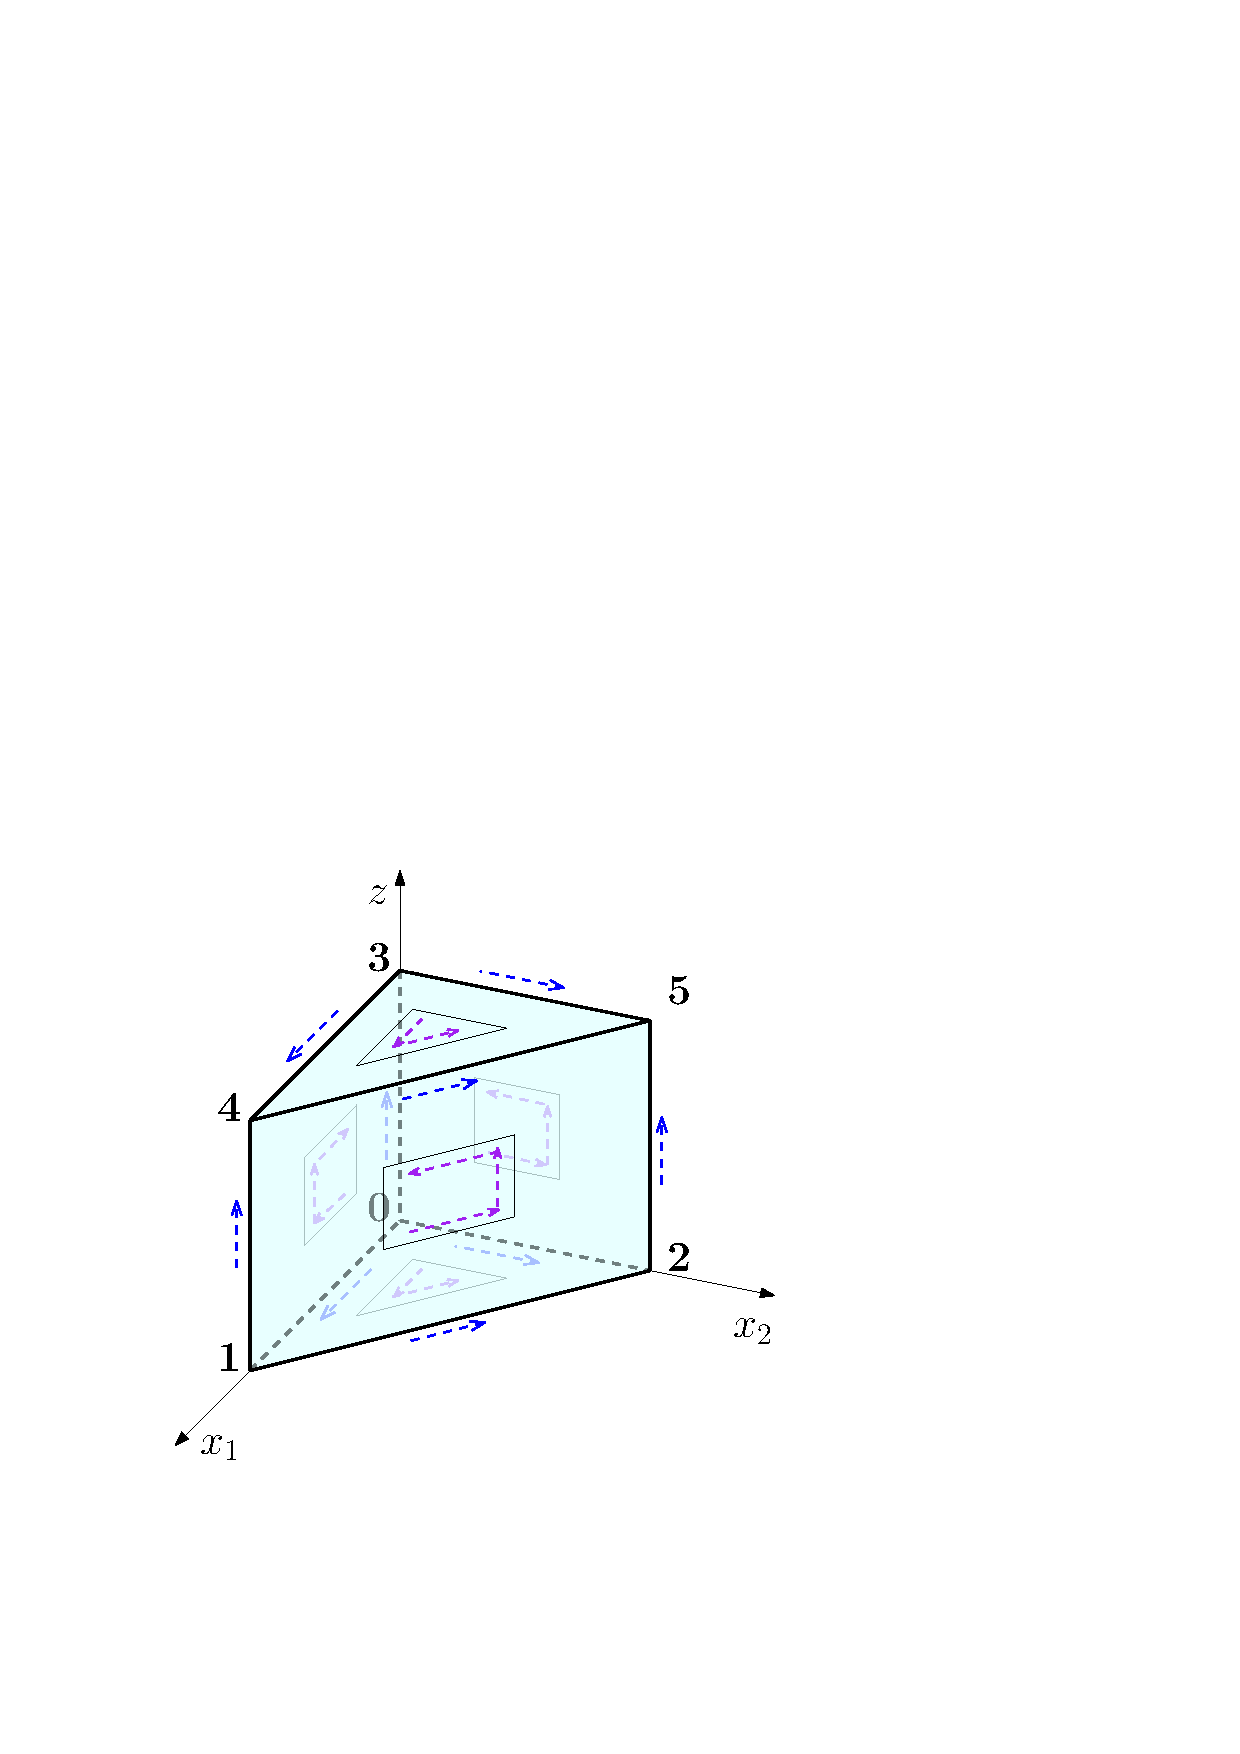
\includegraphics[scale=0.5]{./figures/MasterPrismOrientations.pdf}
\caption{Master prism with numbered vertices \textit{and} local edge and face orientations.}
\label{fig:MasterPrismOrientations}
\end{center}
\end{figure}

To construct orientation embedded shape functions for the prism, it is recommended to have read \S\ref{sec:HexaOrientations} and \S\ref{sec:TetOrientations}.
The predefined \textit{local} edge and face orientations for the prism are illustrated in Figure \ref{fig:MasterPrismOrientations}.
They represent the $\oo=0$ case.
The task at hand is to find the associated \textit{locally ordered} tuples of affine coordinates representing those local orientations.
As usual, the key is being aware of the relationships between the vertices and the affine coordinates.
As examples take edges 01 and 03, and faces 012 and 0143.
%As examples take mixed edge 01, quadrilateral edge 03, triangle face 012 and quadrilateral face 0143.

For mixed edge 01, the vertices are $v_0$ and $v_1$, which are linked to $(\nu_0(x),\mu_0(z))$ and $(\nu_1(x),\mu_0(z))$ respectively.
The only difference is that $v_0$ is linked to $\nu_0(x)$, while $v_1$ is linked to $\nu_1(x)$.
The local orientation for edge 01 is represented by the local vertex-ordering $v_0\tdashto v_1$.
Therefore, the locally ordered pair for edge 01 is $\vec{\nu}_{01}(x)=(\nu_0(x),\nu_1(x))$.
The orientation embedded shape functions for mixed edge 01 are simply the usual shape functions, but with their respective ancillary operator and differential form (that is $\phi_i^\E$, $E_i^\E$, $\nabla\phi_i^\E$ and $\nabla\times E_i^\E$) being precomposed with $\sigma_\oo^\E$ and evaluated at the locally ordered pair.

For quadrilalteral edge 03, composed of vertices $v_0$ and $v_3$, the differing affine coordinates are $\mu_0(z)$ and $\mu_1(z)$ respectively.
Since the local vertex-ordering is $v_0\tdashto v_3$, it follows the locally ordered pair for this edge is $\vec{\mu}_{01}(z)$.
Then, the orientation embedded shape functions are constructed like those of mixed edge 01.
That is, precomposing the ancillary operators with $\sigma_\oo^\E$ and evaluating at the locally ordered pair.

For triangle face 012, composed of vertices $v_0$, $v_1$ and $v_2$, the differing affine coordinates are $\nu_0(x)$, $\nu_1(x)$ and $\nu_2(x)$ respectively.
The local vertex-ordering is $v_0\tdashto v_1\tdashto v_2$, so the locally ordered triplet for this edge is $\vec{\nu}_{012}(x)$.
Then, the orientation embedded shape functions are the usual shape functions but with the ancillary operators ($\phi_{ij}^\Tri$, $E_{ij}^\Tri$, $V_{ij}^\Tri$, $\nabla\phi_{ij}^\Tri$, $\nabla\times E_{ij}^\Tri$ and $\nabla\cdot V_{ij}^\Tri$) precomposed with $\sigma_\oo^\Tri$ and evaluated at the locally oriented triplet.

Finally, quadrilateral face 0143 has local vertex-ordering $v_0\tdashto v_1\tdashto v_4\tdashto v_3$, so one only needs to look at $v_0\tdashto v_1$ and $v_1\tdashto v_4$ as if they were edges.
This leads to the locally ordered pairs $\vec{\nu}_{01}(x)$ and $\vec{\mu}_{01}(z)$ respectively, so the locally ordered quadruple is $(\vec{\nu}_{01}(x),\vec{\mu}_{01}(z))$.
Again, the orientation embedded shape functions are simply the shape functions but with the ancillary operators ($\phi_{ij}^\square$, $E_{ij}^\square$, $V_{ij}^\square$, $\nabla\phi_{ij}^\square$, $\nabla\times E_{ij}^\square$ and $\nabla\cdot V_{ij}^\square$) precomposed with $\sigma_\oo^\square$ and evaluated at the locally oriented quadruple.


%Some info maybe
%The orientations for the prism are dealt much the same way as with the hexahedron and tetrahedron, but in the prism there are two types of edges and two types of faces.
%The two types of edges are treated very similarly, as expected, while the faces are treated separately, since the concept of orientation differs for triangle and quadrilateral faces.
%In any case, the local axes or local numbering, which are fixed at the master element level, are important since they constitute the orientation $\oo=0$ basis case.
%These local axes and numbering are shown in Figure (\textit{add Figure}).%specified in Appendix \ref{app:Enumeration}.
%
%Note that any given vertex is associated to one triangle affine coordinate $\nu_a$ and one edge affine coordinate $\mu_c$, so that indeed its $H^1$ vertex function is precisely $\nu_a\mu_c$ (see \S\ref{sec:PrismH1vertices}).
%The vertices in the bottom triangle face (vertices 0, 1 and 2) are related to $\mu_0$ while those in the top face (vertices 3, 4 and 5) are related to $\mu_1$.
%At the same time, vertices $a$ and $a+3$ are associated to $\nu_a$, for $a=0,1,2$.
%These associations are convenient when explaining the orientations in the case of the prism. 
%
%\subsubsection{Edge Orientations}
%Edge functions, and hence edge orientations are only valid in $H^1$ and $H(\mathrm{curl})$. 
%The treatment is the same for both spaces, with the edge functions $\phi_i^\E$ and $E_i^\E$ being replaced by their oriented versions $\phi_i^{\e,\oo}$ and $E_i^{\e,\oo}$.
%Recall for edges there are only two possible orientations given by the orientation parameter $\oo=0,1$.
%They are explained in \S\ref{sec:edgeorientations}.
%Regardless of the type of edge, the first step is always to look at the local axis, which will determine the order in which the entries are specified in $\phi_i^{\e,\oo}$ and $E_i^{\e,\oo}$, and represents the $\oo=0$ case.
%For completeness, some examples are given below.
%
%\paragraph{Mixed Edges.} Take for example edge 34. 
%Here, vertex 3 is associated to the affine coordinate $\nu_0$, while vertex 4 is related to $\nu_1$. 
%Both are also related to $\mu_1$, since they lie in the top triangle. 
%The local edge axis for this edge points from vertex 3 ($\nu_0$) to vertex 4 ($\nu_1$), meaning that order of the entries in $\phi_i^{\e,\oo}$ and $E_i^{\e,\oo}$ for the mixed edge shape functions associated to this edge should be $(\nu_0(x),\nu_1(x))$. Hence, for instance, the $H^1$ mixed edge shape functions shown in \eqref{eq:PrismH1mixededges} would become
%\begin{equation*}
%	\phi_i^\mathrm{e}=\mu_1\phi_i^{\e,\oo}(\nu_0,\nu_1)
%  	=\begin{cases}
%    	\mu_1\phi_i^{\e,0}(\nu_0,\nu_1)=\mu_1\phi_i^{\e}(\nu_0,\nu_1)\,\,\,\text{if }\oo=0\\
%        \mu_1\phi_i^{\e,1}(\nu_0,\nu_1)=\mu_1\phi_i^{\e}(\nu_1,\nu_0)\,\,\,\text{if }\oo=1\,,
%        \end{cases}
%\end{equation*}
%where $i=2,\ldots,p$. Here, in $\phi_i^{\e,\oo}$, the orientation $\oo=1$ case is managed simply by permuting the indices, as described in \S\ref{sec:edgeorientations}. The same applies to the gradients of these $H^1$ functions and to the $H(\mathrm{curl})$ mixed edge functions and their curl, which involve $E_i^{\e,\oo}$ instead.
%
%\paragraph{Quadrilateral Edges.} Take for example edge 25. 
%Vertices 2 and 5 are related to affine coordinates $\mu_0$ and $\mu_1$ respectively, and both are also related to $\nu_2$.  
%The local axis points from vertex 2 ($\mu_0$) to vertex 5 ($\mu_1$), so that the entries in $\phi_i^{\e,\oo}$ and $E_i^{\e,\oo}$ should be $(\mu_0(z),\mu_1(z))$. 
%More explicitly, the $H^1$ quadrilateral edge shape functions shown in \eqref{eq:PrismH1quadedges} would then be
%\begin{equation*}
%	\phi_i^\mathrm{e}=\nu_2\phi_i^{\e,\oo}(\mu_0,\mu_1)
%  	=\begin{cases}
%    	\nu_2\phi_i^{\e,0}(\mu_0,\mu_1)=\nu_2\phi_i^{\e}(\mu_0,\mu_1)\,\,\,\text{if }\oo=0\\
%        \nu_2\phi_i^{\e,1}(\mu_0,\mu_1)=\nu_2\phi_i^{\e}(\mu_1,\mu_0)\,\,\,\text{if }\oo=1\,,
%        \end{cases}
%\end{equation*}
%where $i=2,\ldots,q$. Again, the same applies to the gradients of these functions and to the $H(\mathrm{curl})$ quadrilateral edge functions and their curl.
%
%\subsubsection{Face Orientations}
%\label{sec:PrismFaceOrientations}
%Face functions (and face orientations) exist in $H^1$, $H(\mathrm{curl})$ and $H(\mathrm{div})$.
%The treatment is analogous for all the spaces, with the triangle face functions $\phi_{ij}^\Tri$, $E_{ij}^\Tri$, $E_{ij}^\Tri}$, and $V_{ij}^\Tri$ and quadrilateral functions $\phi_{ij}^\square$, $E_{ij}^{\square_I}$, $E_{ij}^{\square_{II}}$, and $V_{ij}^\square$, being replaced by their oriented versions $\phi_{ij}^{\Tri,\oo}$, $E_{ij}^{\Tri_I,\oo}$, $E_{ij}^\Tri,\oo}$, $V_{ij}^{\Tri,\oo}$, $\phi_{ij}^{\square,\oo}$, $E_{ij}^{\square_I,\oo}$, $E_{ij}^{\square_{II},\oo}$, and $V_{ij}^{\square,\oo}$. 
%
%\paragraph{Triangle Faces.}
%Triangle face orientations are explained in \S\ref{sec:TriaFaceOrientations}. 
%Here, there are six possible orientations represented by the orientation parameter $\oo=0,\ldots,5$.
%As usual, the first step is to look at the local face numbering.
%For instance, take the top face 345. 
%The vertices 3, 4 and 5 are associated to the affine functions $\nu_0$, $\nu_1$ and $\nu_2$ respectively, and the three are also related to $\mu_1$.
%The local numbering for this face goes from vertex 3 ($\nu_0$) to vertex 4 ($\nu_1$) to vertex 5 ($\nu_2$), so that the order of the entries in  $\phi_{ij}^{\Tri,\oo}$, $E_{ij}^{\Tri_I,\oo}$, $E_{ij}^\Tri,\oo}$, and $V_{ij}^{\Tri,\oo}$ is simply $(\nu_0(x),\nu_1(x),\nu_2(x))$.
%For example, the $H^1$ triangle face shape functions in \eqref{eq:PrismH1TriFace} turn out to be
%\begin{equation*}
%		\phi_{ij}^\mathrm{f}=\mu_1\phi_{ij}^{\Tri,\oo}(\nu_0,\nu_1,\nu_2)=\begin{cases}
%    \mu_1\phi_{ij}^{\Tri}(\nu_0,\nu_1,\nu_2)&\quad\text{if  }\,\oo=0\\
%    \mu_1\phi_{ij}^{\Tri}(\nu_2,\nu_0,\nu_1)&\quad\text{if  }\,\oo=1\\
%    \mu_1\phi_{ij}^{\Tri}(\nu_1,\nu_2,\nu_0)&\quad\text{if  }\,\oo=2\\
%    \mu_1\phi_{ij}^{\Tri}(\nu_0,\nu_2,\nu_1)&\quad\text{if  }\,\oo=3\\
%    \mu_1\phi_{ij}^{\Tri}(\nu_1,\nu_0,\nu_2)&\quad\text{if  }\,\oo=4\\
%    \mu_1\phi_{ij}^{\Tri}(\nu_2,\nu_1,\nu_0)&\quad\text{if  }\,\oo=5\,,
%    \end{cases}
%\end{equation*}
%for $i\geq2$, $j\geq1$ and $n=i+j=3,\ldots,p$. 
%Here, the permutation of the entries depending on the orientation $\oo$ is determined by the auxiliary function $\vec{\sigma}$ which is discussed in \S\ref{sec:TriaFaceOrientations}. 
%Obviously the same arguments apply to the other triangle face functions in $H(\mathrm{curl})$ and $H(\mathrm{div})$ and their differential forms.
%
%\paragraph{Quadrilateral Faces.}
%Quadrilateral face orientations are discussed in \S\ref{sec:QuadFaceOrientations}.
%In this case there are eight possible orientations represented by the orientation parameter $\oo=0,\ldots,7$.
%Take for example face 1254.
%The local numbering goes from vertex 1 (related to $\nu_1$) to vertex 2 (related to $\nu_2$ and $\mu_0$) to vertex 3 (related to $\mu_1$) and to vertex 4.
%Here, the first two elements of the local numbering, vertex 1 with $\nu_1$ to vertex 2 with $\nu_2$, determine the \textit{first} coordinate pair, which is $(\nu_1(x),\nu_2(x))$.
%The second and third elements of the local numbering, vertex 2 with $\mu_0$ to vertex 3 with $\mu_1$, determine the \textit{second} coordinate pair, which is  $(\mu_0(z),\mu_1(z))$.
%These two coordinate pairs constitute the $\oo=0$ orientation, so they are precisely the entries of $\phi_{ij}^{\square,\oo}$, $E_{ij}^{\square_I,\oo}$, $E_{ij}^{\square_{II},\oo}$, and $V_{ij}^{\square,\oo}$. For instance, the $H^1$ quadrilateral shape functions in \eqref{eq:PrismH1QuadFace} become
%\begin{equation*}
%    \phi_{ij}^\mathrm{f}=\phi_{ij}^{\square,\oo}(\nu_1,\nu_2,\mu_0,\mu_1)=\begin{cases}
%    \phi_{ij}^\square(\nu_1,\nu_2,\mu_0,\mu_1)&\quad\text{if  }\,\oo=0\\
%    \phi_{ij}^\square(\mu_1,\mu_0,\nu_1,\nu_2)&\quad\text{if  }\,\oo=1\\
%    \phi_{ij}^\square(\nu_2,\nu_1,\mu_1,\mu_0)&\quad\text{if  }\,\oo=2\\
%    \phi_{ij}^\square(\mu_0,\mu_1,\nu_2,\nu_1)&\quad\text{if  }\,\oo=3\\
%    \phi_{ij}^\square(\mu_0,\mu_1,\nu_1,\nu_2)&\quad\text{if  }\,\oo=4\\
%    \phi_{ij}^\square(\nu_2,\nu_1,\mu_0,\mu_1)&\quad\text{if  }\,\oo=5\\
%    \phi_{ij}^\square(\mu_1,\mu_0,\nu_2,\nu_1)&\quad\text{if  }\,\oo=6\\
%    \phi_{ij}^\square(\nu_1,\nu_2,\mu_1,\mu_0)&\quad\text{if  }\,\oo=7\,,
%    \end{cases}
%\end{equation*}
%where the numbering is $i=2,\ldots,p$, $j=2,\ldots,q$ if $\oo=0,2,5,7$, and $i=2,\ldots,q$, $j=2,\ldots,p$ if $\oo=1,3,4,6$.
%The permutation of the entries is actually determined by the auxiliary function $\vec{\kappa}$ which is explained in \S\ref{sec:QuadFaceOrientations}.
%The same applies to $E_{ij}^{\square_I,\oo}$, $E_{ij}^{\square_{II},\oo}$, $V_{ij}^{\square,\oo}$ and their differential forms.


%Section 9
\newpage
\section{Pyramid}
\label{sec:Pyramid}

\begin{figure}[!ht]
\begin{center}
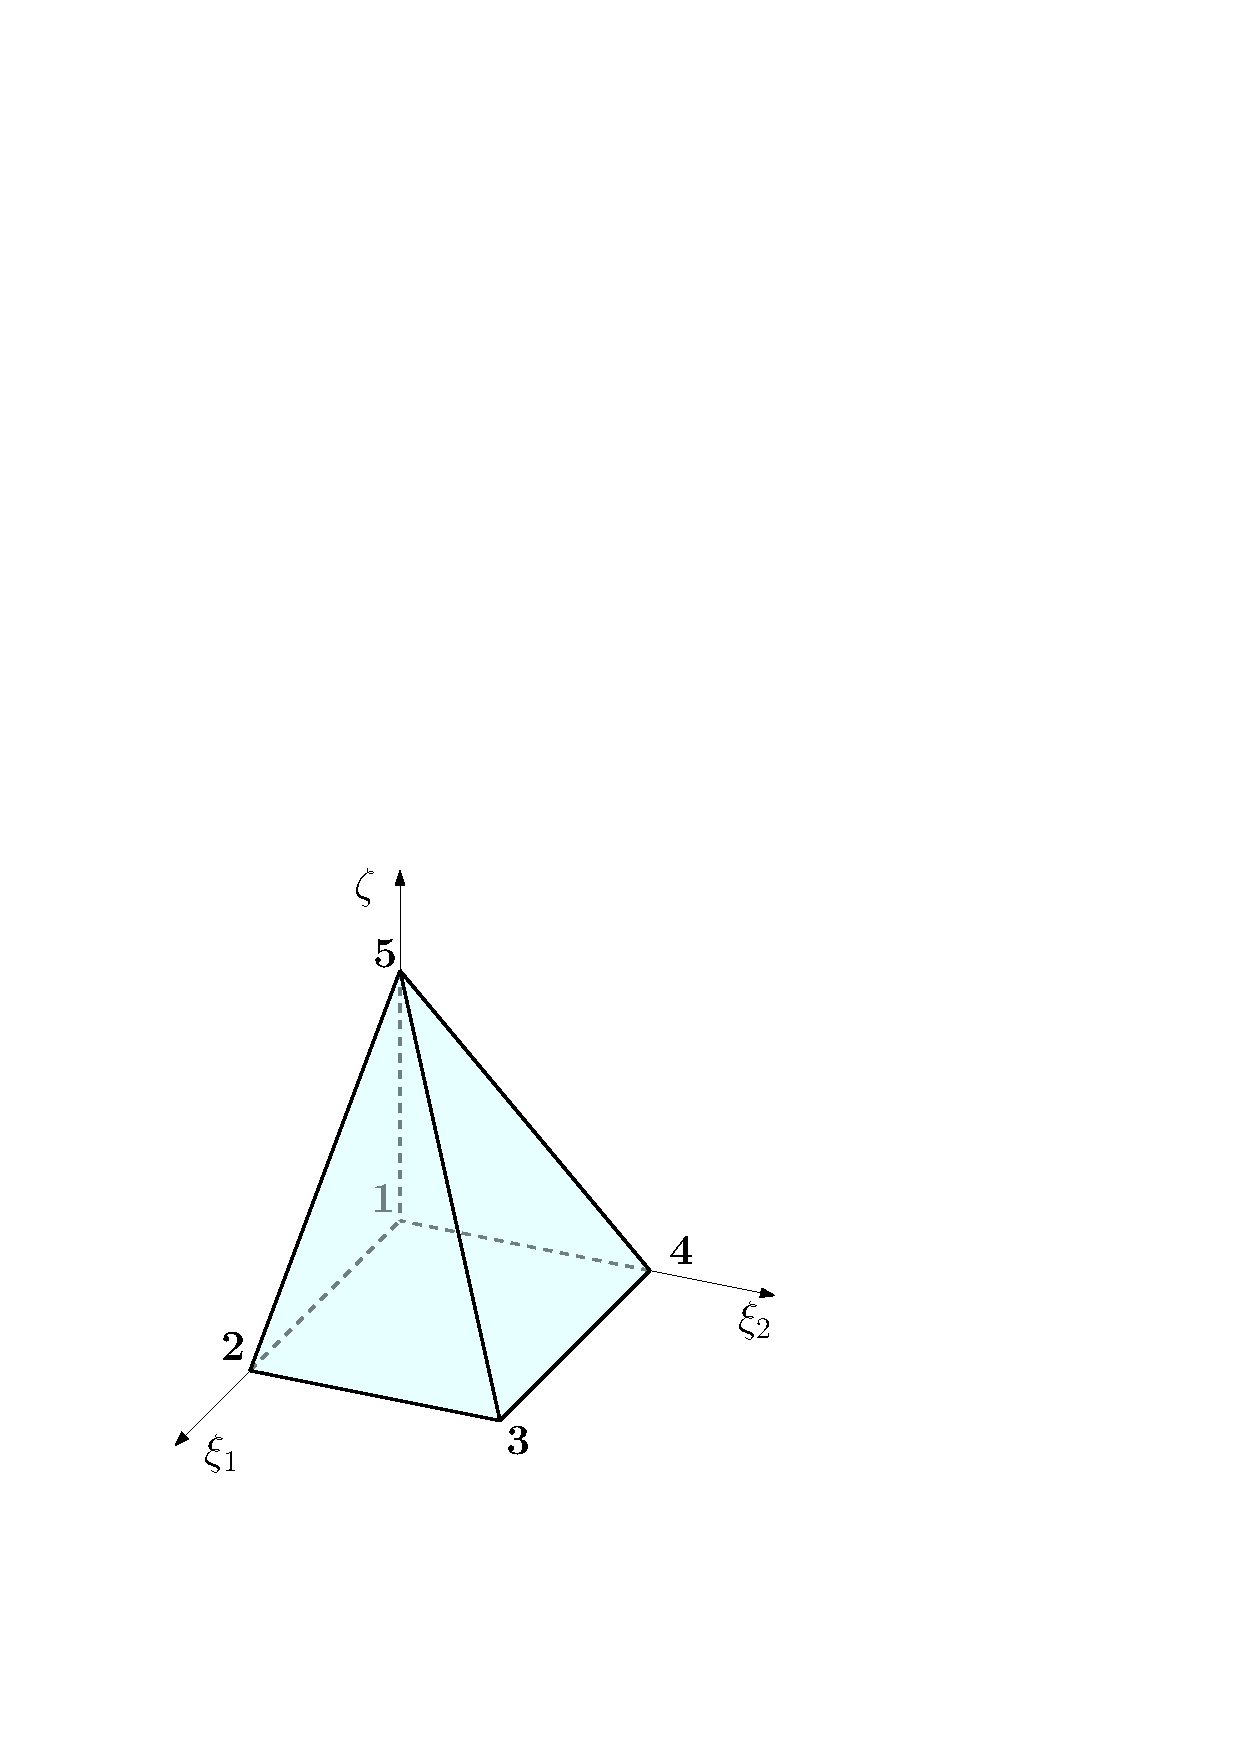
\includegraphics[scale=0.5]{./figures/MasterPyramid.pdf}
\caption{Master pyramid with numbered vertices.}
\label{fig:MasterPyramid}
\end{center}
\end{figure}

The master pyramid is shown in Figure \ref{fig:MasterPyramid} in the $(\xi,\zeta)=(\xi_1,\xi_2,\zeta)$ space.
More specifically, the definition is $\{(\xi_1,\xi_2,\zeta)\in\R^3:\xi_1>0,\xi_2>0,\zeta>0,\xi_1+\zeta<1,\xi_2+\zeta<1\}$.

Clearly, the pyramid is neither a simplex nor a Cartesian product, but it captures features of both quadrilaterals and triangles.
Indeed, it has both quadrilateral and triangle faces. 
Similarly, it has two types of edges. 
Those edges which are adjacent to both a quadrilateral face and a triangle face are called \textit{mixed edges}, while those edges only shared by triangle faces alone are called \textit{triangle edges}. 
These distinctions are fundamental, and the form of the shape functions will differ for the different types of edges and faces.

Due to the virtually unknown structure of the pyramid, at first it seems almost like an insurmountable task to be able to find representative functions that resemble affine coordinates for this 3D element. 
Surprisingly, there is in fact such a set (or rather set\textit{s}) of coordinates.
However, to reach that point, it is better to start by elementary means.
With this in mind, the idea is to separately analyze the affine coordinates of the quadrilateral face and the triangle faces.

In truth, nothing is getting in the way of explicitly computing the 2D triangle affine coordinates of each of the four triangle faces as described in \S\ref{sec:affinecoordinates}.
There turns out to be two independent sets of such coordinates which are
\begin{equation}
	\begin{gathered}
		\nu_0(\xi_1,\zeta)=1-\xi_1-\zeta\,,\qquad\nu_1(\xi_1,\zeta)=\xi_1\,,\qquad\nu_2(\zeta)=\zeta\,,\\
		\nu_0(\xi_2,\zeta)=1-\xi_2-\zeta\,,\qquad\nu_1(\xi_2,\zeta)=\xi_2\,,\qquad\nu_2(\zeta)=\zeta\,.
	\end{gathered}
	\label{eq:PyramidTriCoord}
\end{equation}
Indeed, the triplet $\vec{\nu}_{012}(\xi_1,\zeta)$ represents triangle faces 125 and 435, while the triplet $\vec{\nu}_{012}(\xi_2,\zeta)$ represents triangle faces 145 and 235.
Their gradient is
\begin{equation}
	\begin{gathered}
		\nabla\nu_0(\xi_1,\zeta)=\bigg(\begin{smallmatrix}-1\\[2pt]0\\[2pt]-1\end{smallmatrix}\bigg)\,,\qquad
			\nabla\nu_1(\xi_1,\zeta)=\bigg(\begin{smallmatrix}1\\[2pt]0\\[2pt]0\end{smallmatrix}\bigg)\,,\qquad
				\nabla\nu_2(\zeta)=\bigg(\begin{smallmatrix}0\\[2pt]0\\[2pt]1\end{smallmatrix}\bigg)\,,\\
		\nabla\nu_0(\xi_2,\zeta)=\bigg(\begin{smallmatrix}0\\[2pt]-1\\[2pt]-1\end{smallmatrix}\bigg)\,,\qquad
			\nabla\nu_1(\xi_2,\zeta)=\bigg(\begin{smallmatrix}0\\[2pt]1\\[2pt]0\end{smallmatrix}\bigg)\,,\qquad
				\nabla\nu_2(\zeta)=\bigg(\begin{smallmatrix}0\\[2pt]0\\[2pt]1\end{smallmatrix}\bigg)\,.
	\end{gathered}
	\label{eq:PyramidTriCoordGrad}
\end{equation}

Now, the quadrilateral face can undergo a similar treatment, resulting in the standard two sets of 1D affine coordinates,
\begin{equation*}
	\begin{gathered}
		\mu_0(\xi_1)=1-\xi_1\,,\quad\qquad\mu_1(\xi_1)=\xi_1\,,\\
		\mu_0(\xi_2)=1-\xi_2\,,\quad\qquad\mu_1(\xi_2)=\xi_2\,.
	\end{gathered}
\end{equation*}
However, these are convenient only when restricted to the 2D quadrilateral face, and not in 3D.
The reason is that they do \textit{not} act as blending functions to the \textit{faces}.
For example, $\mu_0(\xi_2)$ is unity at face 125, but it does \textit{not} vanish at the opposite face, which is face 435.
This inconvenience does not occur with the hexahedron or prism due to the Cartesian product structure of those elements.
Despite this setback, it is possible to fix this by considering \textit{scaled} coordinates which additionally depend on $\zeta$.
The sets of quadrilateral scaled 1D affine coordinates are
\begin{equation}
	\begin{gathered}
		\mu_0(\sxi)=1-\sxi\,,\quad\qquad\mu_1(\sxi)=\sxi\,,\\
		\mu_0(\sxii)=1-\sxii\,,\quad\qquad\mu_1(\sxii)=\sxii\,.
	\end{gathered}
	\label{eq:PyramidQuadCoord}
\end{equation}
These can be readily checked to act as \textit{face} blending functions between the opposite triangular faces, which is precisely what was desired.
Moreover, when restricted to the quadrilateral face, so $\zeta=0$, they coincide with the usual sets of affine coordinates for the 2D quadrilateral faces.
Their gradient is
\begin{equation}
	\begin{gathered}
		\nabla\mu_0(\sxi)=\frac{1}{(1-\zeta)^2}\bigg(\begin{smallmatrix}-(1-\zeta)\\[2pt]0\\[2pt]-\xi_1\end{smallmatrix}\bigg)\,,\quad\qquad
    	\nabla\mu_1(\sxi)=\frac{1}{(1-\zeta)^2}\bigg(\begin{smallmatrix}(1-\zeta)\\[2pt]0\\[2pt]\xi_1\end{smallmatrix}\bigg)\,,\\
		\nabla\mu_0(\sxii)=\frac{1}{(1-\zeta)^2}\bigg(\begin{smallmatrix}0\\[2pt]-(1-\zeta)\\[2pt]-\xi_2\end{smallmatrix}\bigg)\,,\quad\qquad
    	\nabla\mu_1(\sxii)=\frac{1}{(1-\zeta)^2}\bigg(\begin{smallmatrix}0\\[2pt](1-\zeta)\\[2pt]\xi_2\end{smallmatrix}\bigg)\,.
	\end{gathered}
	\label{eq:PyramidQuadCoordGrad}
\end{equation}

Lastly, the 1D affine coordinates associated to the nonquadrilateral (top) vertex and the perpendicularly projected point to the quadrilateral face are
\begin{equation}
		\mu_0(\zeta)=1-\zeta\,,\quad\qquad\mu_1(\zeta)=\zeta\,.
		\label{eq:PyramidZCoord}
\end{equation}
Their gradient is
\begin{equation}
		\nabla\mu_0(\zeta)=\bigg(\begin{smallmatrix}0\\[2pt]0\\[2pt]-1\end{smallmatrix}\bigg)\,,\quad\qquad
			\nabla\mu_1(\zeta)=\bigg(\begin{smallmatrix}0\\[2pt]0\\[2pt]1\end{smallmatrix}\bigg)\,.
		\label{eq:PyramidZCoordGrad}			
\end{equation}

With these tools in the arsenal, it is possible to find the desired 3D affine-like coordinates.
The first key observation is that each vertex in the quadrilateral face is associated to \textit{four} lower dimensional affine coordinates.
The associated coordinates are those which take the value $1$ at the given vertex.
For example, vertex $v_1=(0,0,0)$ is linked to the coordinates $\nu_0(\xi_1,\zeta)$, $\nu_0(\xi_2,\zeta)$, $\mu_0(\sxi)$ and $\mu_0(\sxii)$.
To find a global coordinate associated to any vertex, the idea is to combine these components such that they vanish at all disjoint edges and faces.
One possibility is to consider the product of all four coordinates.
However, this gives a high order function, which is somewhat inconsistent with what one would expect.
Hence, the global coordinate should look as ``simple'' as possible.
Fortunately, there is such a coordinate, which in fact has a dual interpretation with respect to its associated coordinates.
It is the product of a 1D scaled affine coordinate and the complementing 2D affine coordinate.
For vertex $v_0$, it would either be $\mu_0(\sxi)\nu_0(\xi_2,\zeta)$ or $\mu_0(\sxii)\nu_0(\xi_1,\zeta)$. 
These two interpretations coincide and define the pyramid affine-related coordinates.
For the nonquadrilateral vertex, $v_5=(0,0,1)$, there is an already existing affine-related coordinate which is merely $\nu_2(\zeta)=\mu_1(\zeta)$.
In summary, the pyramid affine-related coordinates are
\begin{equation}
	\begin{alignedat}{5}
		&\lambda_1(\xi,\zeta)&&=\mu_0(\sxi)\nu_0(\xi_2,\zeta)&&=\mu_0(\sxii)\nu_0(\xi_1,\zeta)
			&&=\textstyle{\frac{(1-\xi_1-\zeta)(1-\xi_2-\zeta)}{1-\zeta}}\,,\\
		&\lambda_2(\xi,\zeta)&&=\mu_1(\sxi)\nu_0(\xi_2,\zeta)&&=\mu_0(\sxii)\nu_1(\xi_1,\zeta)
			&&=\textstyle{\frac{\xi_1(1-\xi_2-\zeta)}{1-\zeta}}\,,\\
		&\lambda_3(\xi,\zeta)&&=\mu_1(\sxi)\nu_1(\xi_2,\zeta)&&=\mu_1(\sxii)\nu_1(\xi_1,\zeta)
			&&=\textstyle{\frac{\xi_1\xi_2}{1-\zeta}}\,,\\
		&\lambda_4(\xi,\zeta)&&=\mu_0(\sxi)\nu_1(\xi_2,\zeta)&&=\mu_1(\sxii)\nu_0(\xi_1,\zeta)
			&&=\textstyle{\frac{(1-\xi_1-\zeta)\xi_2}{1-\zeta}}\,,\\
		&\lambda_5(\zeta)&&=\nu_2(\zeta)&&=\mu_1(\zeta)&&=\zeta\,.
	\end{alignedat}
	\label{eq:PyramidAffineCoord}
\end{equation}
Their gradient is
\begin{equation}
	\begin{gathered}
    \nabla\lambda_1(\xi,\zeta)=\begin{pmatrix}\frac{-(1-\xi_2-\zeta)}{1-\zeta}\\\frac{-(1 -\xi_1-\zeta)}{1-\zeta}\\
        \frac{\xi_1\xi_2}{(1-\zeta)^2}-1\end{pmatrix}\,,\quad
    \nabla\lambda_2(\xi,\zeta)=\begin{pmatrix}\frac{(1-\xi_2-\zeta)}{1-\zeta}\\\frac{-\xi_1}{1-\zeta}\\
        \frac{-\xi_1\xi_2}{(1-\zeta)^2}\end{pmatrix}\,,\quad
    \nabla\lambda_3(\xi,\zeta)=\begin{pmatrix}\frac{\xi_2}{1-\zeta}\\\frac{\xi_1}{1-\zeta}\\
        \frac{\xi_1\xi_2}{(1-\zeta)^2}\end{pmatrix}\,,\\
    \nabla\lambda_4(\xi,\zeta)=\begin{pmatrix}\frac{-\xi_2}{1-\zeta}\\\frac{(1-\xi_1-\zeta)}{1-\zeta}\\
        \frac{-\xi_1\xi_2}{(1-\zeta)^2}\end{pmatrix}\,,\quad
    \nabla\lambda_5(\zeta)=\begin{pmatrix}0\\0\\1\end{pmatrix}\,.
	\end{gathered}
	\label{eq:PyramidAffineCoordGrad}
\end{equation}

Apart from being products of lower dimensional affine coordinates, the pyramid affine-related coordinates truly do behave in many ways like 3D affine coordinates.
Firstly, notice that by construction the traces over adjacent faces and edges are the corresponding vertex functions of those lower dimensional topological entities.
For example, the trace of $\lambda_1$ over faces 125 and 145 is a 2D triangle affine coordinate associated to that vertex, while that of face 1234 is a bilinear quadrilateral vertex function.
Secondly, note that every $(\xi,\zeta)$ in the pyramid can be expressed as a convex combination of the vertices with the affine coordinates being the weights,
\begin{equation}
	\bigg(\begin{smallmatrix}\xi_1\\[2pt]\xi_2\\[2pt]\zeta\end{smallmatrix}\bigg)=\sum_{a=1}^5 \lambda_a(\xi,\zeta)v_a\,,
		\qquad\quad\text{ with }\quad\sum_{a=1}^5 \lambda_a(\xi,\zeta)=1\,\;\text{ and }\; 0\leq\lambda_a(\xi,\zeta)\leq1\,,
\end{equation}
and where $v_a$ are the coordinates of vertex $a$. 
The main difference with the legitimate simplex affine coordinates radicates in the fact the the pyramid affine-related coordinates are not \textit{defined} by the properties above (see \S\ref{sec:affinecoordinates}).
Indeed, even though they have polynomial traces at the boundary, they involve rational polynomials in the interior, and this is an inherently new property.
Nevertheless, for many practical purposes, they can be thought of as affine coordinates, and from now on will be referred to as \textit{the} pyramid affine coordinates.

An important remark is that all the results associated to the definitions of the ancillary functions were proved in a very general setting that encompasses the pyramid affine coordinates and the fact they can be rational. 
In particular, the proofs of Lemmas \ref{lem:curlformula} and \ref{lem:divformula} hold.

Note that all the affine coordinates illustrated can be computed for pyramids with a parallelogram base.
In fact, it is very easy to make these calculations for pyramids with an arbitrarily placed top vertex and whose rectangular base is normal to the vertical $\zeta$ direction and aligned with the $\xi$ coordinates.
This assertion includes any of the typical master pyramids found in the literature.
With the affine coordinates computed, it is just a matter of substituting them (and their gradient) into the expressions for the shape functions to be presented throughout this section, so that in fact these expressions are independent of the choice of the master pyramid.
Hopefully, this motivates other researchers to communicate their results in terms of affine coordinates as well.

Finally, by construction, there are natural relationships between the topological entities and the different types of affine coordinates defined.
The related affine coordinates are those which take the value $1$ at the prescribed topological entity.
The top vertex, $v_5$, is linked to $\nu_2(\zeta)=\mu_1(\zeta)=\lambda_5(\zeta)$.
The quadrilateral vertices are each associated to \textit{two} 1D scaled affine coordinates, \textit{two} 2D triangle affine coordinates and \textit{one} 3D pyramid affine coordinate.
Meanwhile, triangle edges are linked to \textit{two} 1D scaled affine coordinates, while mixed edges are associated to \textit{one} 1D scaled affine coordinate and the vertical 1D affine coordinate $\mu_0(\zeta)$.
Lastly, triangle faces are linked to \textit{one} 1D scaled affine coordinate, while the quadrilateral face is linked to the vertical 1D affine coordinate $\mu_0(\zeta)$.
As usual, these associated affine coordinates can act as natural blending functions.

\subsubsection*{Exact Sequence}

It should be clear by now that the pyramid has a fundamentally different structure than the previous elements, and one would expect this to have an impact on the discrete spaces that attempt to approximate the energy spaces in \eqref{eq:3D_exact_sequence}.

Firstly, note that an absolute requirement is that the trace of the spaces over the faces span the lower dimensional discrete polynomial spaces for the triangle and quadrilateral respectively.
This is what ensures that the shape functions are compatible over adjacent elements.
However, any attempt at finding a three dimensional polynomial space satisying those properties is futile, since one can find counterexamples mathematically showing that this task is impossible.

Hence, the use of \textit{rational} polynomial spaces is the next natural step.
This issue already arised, at least intuitively, while analyzing the desired properties of affine coordinates, because the use of \textit{scaled} coordinates was required.
Nevertheless, dealing with rational polynomial spaces is difficult, and finding finite dimensional higher order spaces satisfying all the desired trace, exact sequence and approximability properties is a far from trivial task.
In fact, only until recently did such constructions started to appear in the literature.
In the context of this work, perhaps the best suited set of such spaces is that proposed by \citet{Nigam_Phillips_11}, which is consistent with the ``natural'' first order spaces analyzed first by \citet{Hiptmair99}.

Respecting the notation of \citet{Nigam_Phillips_11}, the discrete rational polynomial spaces approximating \eqref{eq:3D_exact_sequence} are,
\begin{equation}
	\mathcal{U}^{(0),p} \xrightarrow{\,\,\nabla\,\,} \mathcal{U}^{(1),p} \xrightarrow{\nabla\times} 
	\mathcal{U}^{(2),p} \xrightarrow{\nabla\cdot} \mathcal{U}^{(3),p} \,,
	\label{eq:pyramidsequence}
\end{equation}
where the $m$ in $\mathcal{U}^{(m),p}$ corresponds to the order of the differential form in 3D, so that the elements in $\mathcal{U}^{(0),p}$ are $0$-forms, and so on.
The precise definitions of these spaces are somewhat technical and will be postponed to Appendix \ref{app:pyrappendix}.
In fact, the proofs that the shape funtions lie in the desired space are also technical and inconveniently load the readibility of the document, so they are presented in Appendix \ref{app:pyrappendix} as well. 
This by no means implies that the spaces are not important and do not play a role in the construction.
In fact, quite the opposite.
The spaces are so well suited to the pyramid, that most of the time they impose little restrictions on the intuitive constructions presented here.
Hence, in many ways, despite looking complicated, they are ``natural''.

Finally, it is worth emphasizing that the goal in this section (and in general in this work) is to motivate the construction of the shape functions through geometrical arguments (via the affine coordinates defined before) combined with the carefully chosen ancillary operators defined throughout the document.
This approach leads to shape functions satisfying the desired trace properties and which either are in the desired space or can be naturally tweaked to lie in the space.
The notable exception is that of the $H(\mathrm{div})$ triangle faces, in which the space truly plays a nontrivial role and forces to consider a more intricate yet consistent construction.

%Having said this, there are exceptions.
%Notably, in the case of $H(\mathrm{div})$, the space truly plays a nontrivial role and forces to consider a more intricate construction for some shape functions.
%These exceptions will be pointed out.

%Hence, the focus will be on the geometric intuition and on how the logic of projecting, evaluating and blending applies to the shape functions in this element.
%The desired trace properties


%This approach leads to shape functions which are in the desired space or which can be intuitively modified to lie in the space.
%Hence, this speaks very well on the suitability and importance of these spaces for the pyramid, which in many ways can be considered `natural'.
%Having said this, there are exceptions.
%Notably, in the case of $H(\mathrm{div})$, the space truly plays a nontrivial role and forces to consider a more intricate construction for some shape functions.
%These exceptions will be pointed out.
%
%This by no means implies that 
%
%
%will all be given in Appendix \ref{app:pyrappendix}.
%
%The justification for this is that the construction of shape functions is fully motivated by geometrical arguments (via the affine coordinates defined before) combined with the carefully chosen ancillary operators defined throughout the document.
% 
%Hence, in many ways the space plays a `natural' role and imposes little restrictions on the construction.
%This speaks very well on the suitability of these spaces for the pyramid.
%However, the proofs that the shape functions are in the space are technical and inconveniently load the readibility of the document, which has the goal of motivating the shape functions through
%, that the aspect of conformability almost becomes superfluous.  
%This , but it is inconvenient to load the readibility of these proofs on of the document, they are given in Appendix \ref{app:pyrappendix}.
%Having said this, there are key exceptions in the case of $H(\mathrm{div})$, where the space truly plays a nontrivial role and forces to consider a more intricate construction.
%These exceptions will be pointed out.

\subsection{\texorpdfstring{$H^1$}{H1} Shape Functions}

The dimension of the space $\mathcal{U}^{(0),p}$ is $p^3+3p+1$.
The number of linearly independent shape functions will coincide with that dimension.

\subsubsection {\texorpdfstring{$H^1$}{H1} Vertices}

The vertex shape functions will be precisely the associated 3D pyramid affine coordinates.
Indeed, take for example vertex $v_1$, so that the vertex function is
\begin{equation*}
	\phi^\mathrm{v}(\xieta)=\lambda_1(\xieta)\,.
\end{equation*}
The trace properties are satisfied by construction and are shown explicitly next,
\begin{equation*}
	\begin{alignedat}{5}
    &\phi^\mathrm{v}(\xieta)|_{\xi_2=0}&&=\lambda_1(\xieta)|_{\mu_0(\frac{\xi_1}{1-\zeta})=1}
    	&&=\mu_0(\sxi)\nu_0(\xi_2,\zeta)|_{\mu_0(\frac{\xi_1}{1-\zeta})=1}&&=\nu_0(\xi_2,\zeta)\,,\\
    &\phi^\mathrm{v}(\xieta)|_{\xi_1=1-\zeta}&&=\lambda_1(\xieta)|_{\mu_0(\frac{\xi_2}{1-\zeta})=0}
    	&&=\mu_0(\sxii)\nu_0(\xi_1,\zeta)|_{\mu_0(\frac{\xi_2}{1-\zeta})=0}&&=0\,,\\
  	&\phi^\mathrm{v}(\xieta)|_{\xi_2=1-\zeta}&&=\lambda_1(\xieta)|_{\mu_0(\frac{\xi_1}{1-\zeta})=0}
    	&&=\mu_0(\sxi)\nu_0(\xi_2,\zeta)|_{\mu_0(\frac{\xi_1}{1-\zeta})=0}&&=0\,,\\
    &\phi^\mathrm{v}(\xieta)|_{\xi_2=0}&&=\lambda_1(\xieta)|_{\mu_0(\frac{\xi_2}{1-\zeta})=1}
    	&&=\mu_0(\sxii)\nu_0(\xi_1,\zeta)|_{\mu_0(\frac{\xi_2}{1-\zeta})=1}&&=\nu_0(\xi_1,\zeta)\,,\\
    &\phi^\mathrm{v}(\xieta)|_{\zeta=0}&&=\lambda_1(\xieta)|_{\zeta=0}
    	&&=\mu_0(\xi_1)\mu(\xi_2)\,.&&\\
	\end{alignedat}
\end{equation*}
The function is also in the lowest order space $\mathcal{U}^{(0),1}$.
Similar arguments apply to all other quadrilateral vertices and the top vertex as well.

More generally, the vertex functions and their gradient are,
\begin{equation}
    \phi^\mathrm{v}(\xieta)=\lambda_a(\xieta)\,,\qquad\quad\nabla\phi^\mathrm{v}(\xieta)=\nabla\lambda_a(\xieta)\,,
    \label{eq:PyrH1Vertex}
\end{equation}
for $a=1,2,3,4,5$.
There are a total of $5$ vertex functions (one for each vertex).

\subsubsection{\texorpdfstring{$H^1$}{H1} Edges}

\paragraph{\texorpdfstring{$H^1$}{H1} Mixed Edges.} 
Take for example mixed edge 12.
The first naive approach is to use the 3D pyramid affine coordinates directly on $\phi_i^\E$, which gives
\begin{equation*}
	\phi_i^\mathrm{e}(\xieta)=\phi_i^\E(\vec{\lambda}_{12}(\xieta))
		=\phi_i^\E\Big(\mu_0(\sxii)\nu_0(\xi_1,\zeta),\mu_0(\sxii)\nu_1(\xi_1,\zeta)\Big)
			=\mu_0(\sxii)^i\phi_i^\E(\vec{\nu}_{01}(\xi_1,\zeta))\,,
\end{equation*}
for $i=2,\ldots,p$.
This attempt almost works because it is in the correct space, satisfies the vanishing conditions, and even has the right form at the edge itself.
Indeed, at triangle faces 235 and 145, $\nu_0(\xi_1,\zeta)=0$ and $\nu_1(\xi_1,\zeta)=0$ respectively, while $\mu_0(\sxii)=0$ at face 435.
However, the nonzero trace over the adjacent quadrilateral face is not of the correct form, since it blends nonlinearly with the factor $\mu_0(\xi_2)^i$ instead of linearly like $\mu_0(\xi_2)$.
Therefore the function violates dimensional hierarchy and does not work for our purposes.
Nevertheless this analysis ellucidates how to fix the issue.
The idea is to have the factor $\mu_0(\sxii)$ separated as a blending factor, so that the effects of $\mu_0(\sxii)$ are essentially separated from those of $\vec{\nu}_{01}(\xi_1,\zeta)$ in $\vec{\lambda}_{12}(\xieta)$.
%This can always be done because of the decomposition of the 3D pyramid affine coordinate into lower dimensional affine coordinates.
Hence, the shape functions for this edge are
\begin{equation*}
	\phi_i^\mathrm{e}(\xieta)=\mu_0(\sxii)\phi_i^\E(\vec{\nu}_{01}(\xi_1,\zeta))=
		\underbrace{\mu_0(\sxii)(\nu_0(\xi_1,\zeta)+\nu_1(\xi_1,\zeta))^i}_{\text{blend}}
    	\underbrace{\phi_i^\E\Big(\underbrace{\textstyle{\frac{1}{\nu_0(\xi_1,\zeta)+\nu_1(\xi_1,\zeta)}}
    		\vec{\nu}_{01}(\xi_1,\zeta)}_{\text{project}}\Big)}_{\text{evaluate}}\,,
\end{equation*}
for $i=2,\ldots,p$.
As with the previous candidate all vanishing properties are satisfied, but this time the nonzero trace properties are also easily seen to hold.
The projection being implied is
\begin{equation*}
	(\xi_1,\xi_2,\zeta)\;\longmapsto\;\begin{matrix}(\xi_1,0,\zeta)\\(\sxi,\sxii,0)\end{matrix}
		\;\longmapsto\;(\sxi,0,0)\,.
\end{equation*}
It is a two step projection, where the first step is to project to an adjacent face and the second is to project along that face to the given edge via the standard 2D edge projections (see Figures \ref{fig:QuadProjection} and \ref{fig:TriangleProjection}).
If the face projection is chosen as the triangle, then the projection at play is called the \textit{horizontal} triangle face projection and consists of finding the intersection $P'=(\xi_1,0,\zeta)$ of the face with the projecting line parallel to the $\xi_2$ direction and passing through the original point $P=(\xi_1,\xi_2,\zeta)$. 
This is shown in Figure \ref{fig:PyramidProjectionHorizontalTriangle}.
If the face projection is chosen as the quadrilateral, then the projection is simply the intersection $P'=(\sxi,\sxii,0)$ of the face with the projecting line passing through the top vertex and the original point $P=(\xi_1,\xi_2,\zeta)$. 
This is shown in Figure \ref{fig:PyramidProjectionQuad}.

\begin{figure}[!ht]
\begin{center}
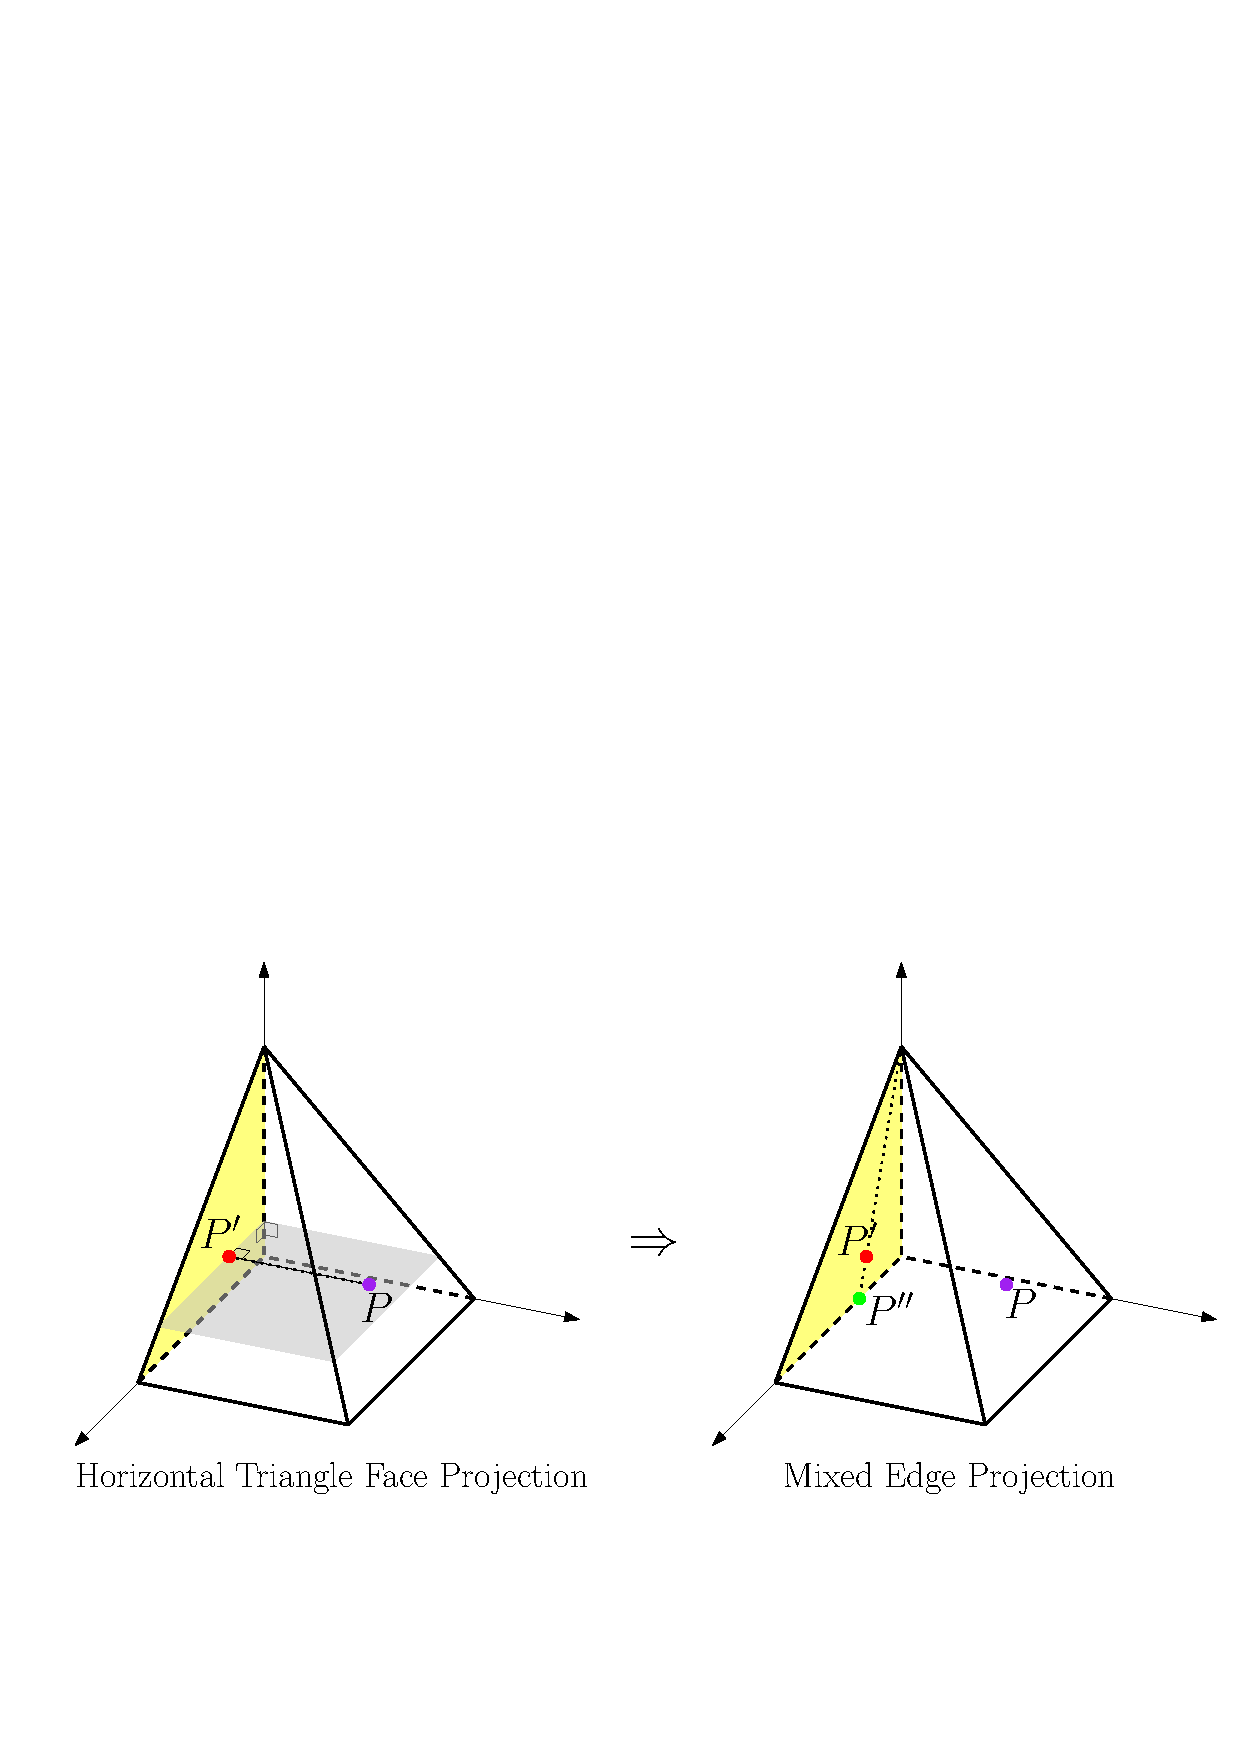
\includegraphics[scale=0.6]{./figures/PyramidProjectionHorizontalTriangle.pdf}
\caption{Horizontal triangle face projection from $P$ to $P'$ followed by a mixed edge projection from $P'$ to $P''$.}
\label{fig:PyramidProjectionHorizontalTriangle}
\end{center}
\end{figure}

In general, the shape functions and their gradient are
\begin{equation}
	\begin{aligned}
		\phi_i^\mathrm{e}(\xieta)&=\mu_c(\sxib)\phi_i^\E(\vec{\nu}_{01}(\xi_a,\zeta))\,,\\
    	\nabla\phi_i^\mathrm{e}(\xieta)&=\mu_c(\sxib)\nabla\phi_i^\E(\vec{\nu}_{01}(\xi_a,\zeta))
        +\phi_i^\E(\vec{\nu}_{01}(\xi_a,\zeta))\nabla\mu_c(\sxib)\,,	
	\end{aligned}
	\label{eq:PyrH1MixedEdge}
\end{equation}
where $i=2,\ldots,p$, $(a,b)=(1,2),(2,1)$ and $c=0,1$.
There are $p-1$ edge function for each edge, for a total of $4(p-1)$ mixed edge functions.

\paragraph{\texorpdfstring{$H^1$}{H1} Triangle Edges.}
For instance, take triangle edge 15.
Again, the naive approach is to use the 3D pyramid affine coordinates on $\phi_i^\E$, leading to the shape functions,
\begin{equation*}
	\phi^\mathrm{e}(\xieta)=\phi_i^\E(\vec{\lambda}_{15}(\xieta))=
		\underbrace{(\lambda_1(\xieta)+\lambda_5(\zeta))^i}_{\text{blend}}
    	\underbrace{\phi_i^\E\Big(\underbrace{\textstyle{\frac{1}{\lambda_1(\xieta)+\lambda_5(\zeta)}}
    		\vec{\lambda}_{15}(\xieta)}_{\text{project}}\Big)}_{\text{evaluate}}\,,
\end{equation*}
for $i=2,\ldots,p$.
In this case it works perfectly well, with the trace properties being satisfied.
Indeed, $\lambda_1(\xieta)=0$ over faces 235 and 435, while $\lambda_5(\xieta)=0$ over the quadrilateral face.
Moreover the restriction of $\vec{\lambda}_{15}(\xieta)$ over the faces 125 and 145 gives $\vec{\nu}_{02}(\xi_1,\zeta)$ and $\vec{\nu}_{02}(\xi_2,\zeta)$ respectively, so the nonzero traces are the appropriate triangle traces.
The projection being implied here is highly nontrivial. 
It is a two step projection given by
\begin{equation*}
	(\xi_1,\xi_2,\zeta)\;\longmapsto\;\Big(\textstyle{\frac{\xi_1(1-\xi_2-\zeta)}{(1-\xi_2)(1-\zeta)}},
		0,\textstyle{\frac{\zeta}{1-\xi_2}}\Big)\;\longmapsto\;
			\Big(0,0,\textstyle{\frac{\zeta(1-\zeta)}{(1-\xi_1-\zeta)(1-\xi_2-\zeta)+\zeta(1-\zeta)}}\Big)\,.
\end{equation*}
The first step is called an \textit{oblique} triangle face projection and consists of running a plane through the original point $P=(\xi_1,\xi_2,\zeta)$ and the opposite bottom edge to the face (edge 43), followed by finding the intersection of this plane with the planes passing through the other two adjacent triangular faces (faces 235 and 415 with equations $\xi_1=1-\zeta$ and $\xi_1=0$ respectively).
Call this intersection $C=(0,-(\frac{1-\xi_2-\zeta}{\zeta}),1)$.
Finally, the intersection of face 125 with the projecting line from the original point $P$ to the intersection $C$ is found and labeled as $P'=(\frac{\xi_1(1-\xi_2-\zeta)}{(1-\xi_2)(1-\zeta)},0,\frac{\zeta}{1-\xi_2})$.
This projection is illustrated in Figure \ref{fig:PyramidProjectionObliqueTriangle}.
The final step is simply to project as usual along the 2D triangle face to the point $P''=(0,0,\frac{\zeta(1-\zeta)}{(1-\xi_1-\zeta)(1-\xi_2-\zeta)+\zeta(1-\zeta)})$.

\begin{figure}[!ht]
\begin{center}
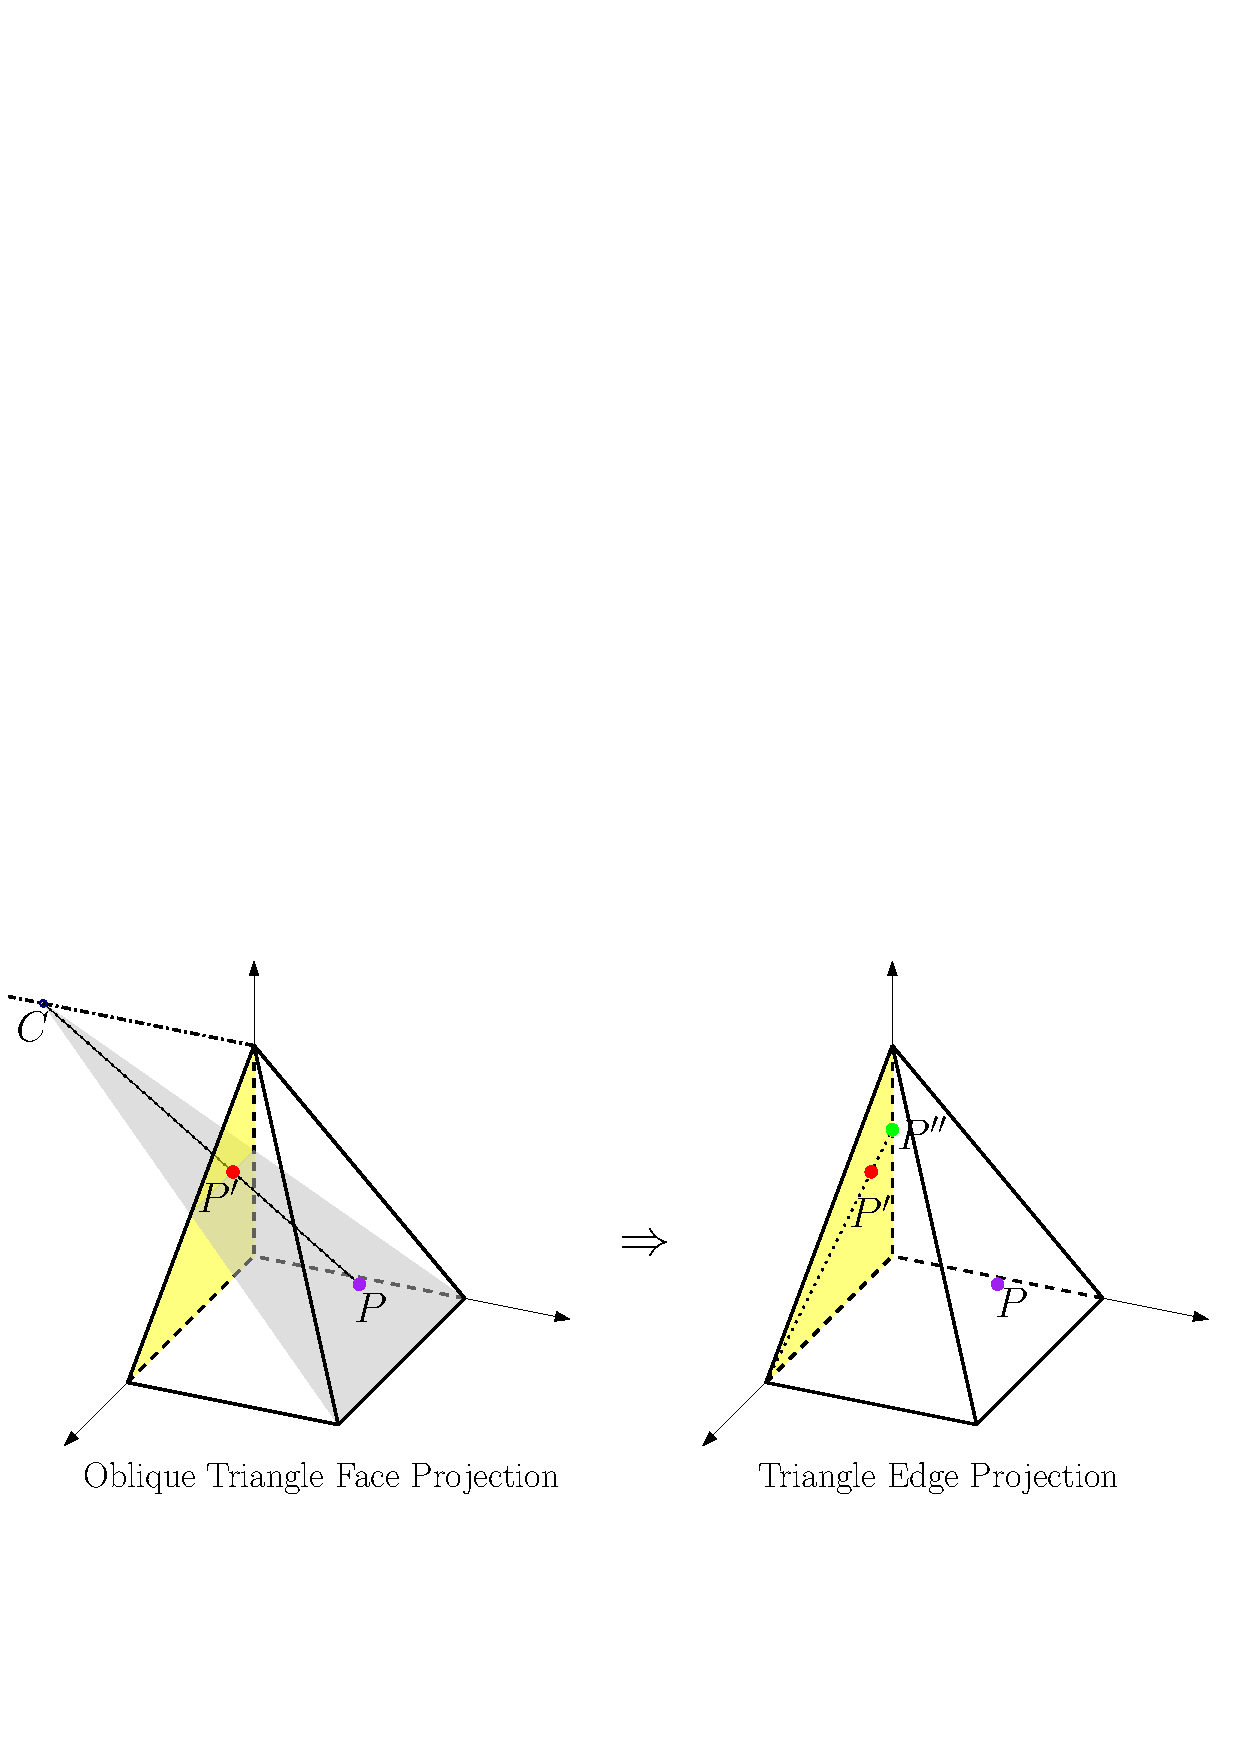
\includegraphics[scale=0.6]{./figures/PyramidProjectionObliqueTriangle.pdf}
\caption{Oblique triangle face projection from $P$ to $P'$ followed by a triangle edge projection from $P'$ to $P''$.}
\label{fig:PyramidProjectionObliqueTriangle}
\end{center}
\end{figure}

In general, the shape functions and their gradient are
\begin{equation}
	\phi_i^\mathrm{e}(\xieta)=\phi_i^\E(\vec{\lambda}_{a5}(\xieta))\,,\qquad\quad
	\nabla\phi_i^\mathrm{e}(\xieta)=\nabla\phi_i^\E(\vec{\lambda}_{a5}(\xieta))\,,
	\label{eq:PyrH1TriaEdge}
\end{equation}
for $i=2,\ldots,p$ and $a=1,2,3,4$.
There are $p-1$ edge functions for each edge, giving a total of $4(p-1)$ triangle edge functions.


\subsubsection{\texorpdfstring{$H^1$}{H1} Faces}

\begin{figure}[!ht]
\begin{center}
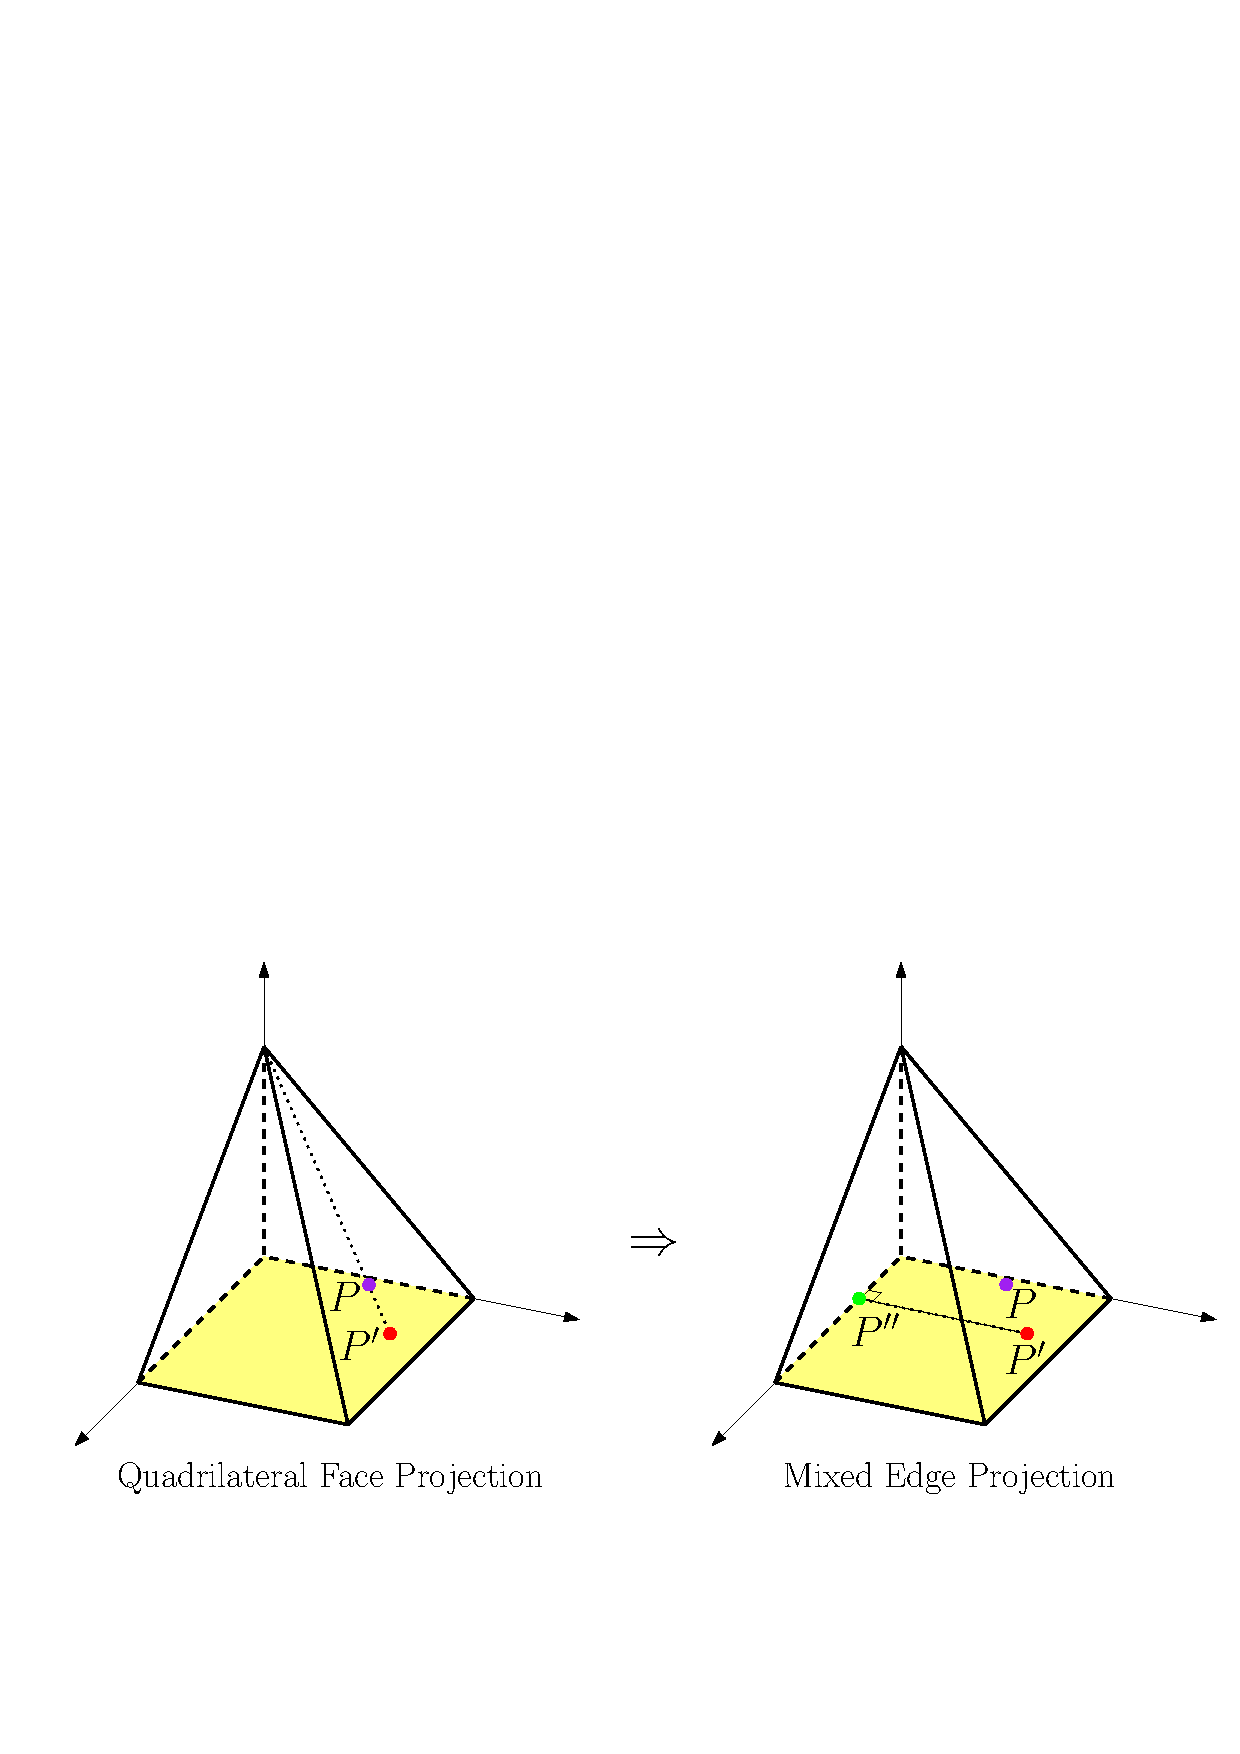
\includegraphics[scale=0.6]{./figures/PyramidProjectionQuad.pdf}
\caption{Quadrilateral face projection from $P$ to $P'$ followed by a mixed edge projection from $P'$ to $P''$.}
\label{fig:PyramidProjectionQuad}
\end{center}
\end{figure}

\paragraph{\texorpdfstring{$H^1$}{H1} Quadrilateral Face.} 
It was already mentioned that the quadrilateral face projection, illustrated in Figure \ref{fig:PyramidProjectionQuad}, takes an arbitrary point $P=(\xi_1,\xi_2,\zeta)$ to the point $P'=(\sxi,\sxii,0)$ along the face. This projected point is actually represented by the affine coordinate quadruple $(\vec{\mu}_{01}(\sxi),\vec{\mu}_{01}(\sxii))$. 
Hence, the natural choice is to use the quadruple with the ancillary function $\phi_{ij}^\square$. 
This already satisfies all the necessary trace properties, except at the top vertex itself, where there might be a singularity.
This is corrected by adding a factor of $\mu_0(\zeta)$, which also ensures the function is in the correct space.

The shape functions and their gradient are
\begin{equation}
	\begin{aligned}
		\phi_{ij}^\mathrm{f}(\xieta)&=\mu_0(\zeta)\phi_{ij}^\square\Big(\vec{\mu}_{01}(\sxi),\vec{\mu}_{01}(\sxii)\Big)\,,\\
    	\nabla\phi_{ij}^\mathrm{f}(\xieta)&=\mu_0(\zeta)\nabla\phi_{ij}^\square\Big(\vec{\mu}_{01}(\sxi),\vec{\mu}_{01}(\sxii)\Big)
        +\phi_{ij}^\square\Big(\vec{\mu}_{01}(\sxi),\vec{\mu}_{01}(\sxii)\Big)\nabla\mu_0(\zeta)\,,	
	\end{aligned}
	\label{eq:PyrH1QuadFace}
\end{equation}
where $i=2,\ldots,p$ and $j=2,\ldots,p$. 
Naturally, there are $(p-1)^2$ shape functions for the quadrilateral face.

\paragraph{\texorpdfstring{$H^1$}{H1} Triangle Faces.} 
Similar to the mixed edges, there are two possibilities.
Obviously they both involve $\phi_{ij}^\Tri$.
Take for example triangle face 125.
The first alternative is to use the 3D pyramid affine coordinates directly, yielding as a result
\begin{equation*}
	\phi_{ij}^\mathrm{f}(\xieta)=\phi_{ij}^\Tri(\vec{\lambda}_{125}(\xieta))=
		\underbrace{(\lambda_1(\xieta)+\lambda_2(\xieta)+\lambda_5(\zeta))^{i+j}}_{\text{blend}}
    	\underbrace{\phi_{ij}^\Tri\Big(\underbrace{\textstyle{\frac{1}{\lambda_1(\xieta)+\lambda_2(\xieta)+\lambda_5(\zeta)}}
    		\vec{\lambda}_{125}(\xieta)}_{\text{project}}\Big)}_{\text{evaluate}}\,,
\end{equation*}
where $i\geq2$ and $j\geq1$.
In this case the projection implied is precisely the oblique triangle face projection illustrated in Figure \ref{fig:PyramidProjectionObliqueTriangle}.
This function lies in the correct space and is easily seen to satisfy the necessary trace properties (see \eqref{eq:phiTrivanishing}).
Hence, it is a perfectly valid candidate.

A second candidate relies in the same approach taken for the mixed edges, in which the effects of the components of $\vec{\lambda}_{12}(\xieta)$ are separated. 
In that case, the functions are
\begin{equation*}
		\phi_{ij}^\mathrm{f}(\xieta)=\underbrace{\mu_0(\sxii)}_{\text{blend}}
    	\underbrace{\phi_{ij}^\Tri\Big(\underbrace{\vec{\nu}_{012}(\xi_1,\zeta)}_{\text{project}}\Big)}_{\text{evaluate}}\,,
\end{equation*}
for $i\geq2$ and $j\geq1$.
Here, the projection implied is the horizontal triangle face projection shown in Figure \ref{fig:PyramidProjectionHorizontalTriangle}.
Again, the function is in the correct space and satisfies the required trace properties, so it is also a valid candidate.

The second alternative is chosen, so the general shape functions and their gradient are
\begin{equation}
	\begin{aligned}
		\phi_{ij}^\mathrm{f}(\xieta)&=\mu_c(\sxib)\phi_{ij}^\Tri(\vec{\nu}_{012}(\xi_a,\zeta))\,,\\
    	\nabla\phi_{ij}^\mathrm{f}(\xieta)&=\mu_c(\sxib)\nabla\phi_{ij}^\Tri(\vec{\nu}_{012}(\xi_a,\zeta))
        +\phi_{ij}^\Tri(\vec{\nu}_{012}(\xi_a,\zeta))\nabla\mu_c(\sxib)\,,	
	\end{aligned}
	\label{eq:PyrH1TriaFace}
\end{equation}
where $i\geq2$, $j\geq1$, $n=i+j=3,\ldots,p$, $(a,b)=(1,2),(2,1)$ and $c=0,1$.
As with all $H^1$ triangle edges, there are $\frac{1}{2}(p-1)(p-2)$ face functions for each face, for a total of $2(p-1)(p-2)$ triangle face functions.

\subsubsection{\texorpdfstring{$H^1$}{H1} Interior Bubbles}

The interior bubble functions resemble closely the case of the hexahedron bubbles, and they are deduced from the quadrilateral face functions, where the factor $\phi_k^\E(\vec{\mu}_{01}(\zeta))$ is used instead of $\mu_0(\zeta)$.
This ensures all the vanishing properties are satisfied.

The bubble functions and their gradient are
\begin{equation}
	\begin{aligned}
		\phi_{ijk}^\mathrm{b}(\xieta)&\!=\!
			\phi_{ij}^\square\Big(\vec{\mu}_{01}(\sxi),\vec{\mu}_{01}(\sxii)\Big)\phi_k^\E(\vec{\mu}_{01}(\zeta))\,,\\
    		\nabla\phi_{ijk}^\mathrm{b}(\xieta)&\!=\!\phi_k^\E(\vec{\mu}_{01}(\zeta))
    			\nabla\phi_{ij}^\square\Big(\vec{\mu}_{01}(\sxi),\vec{\mu}_{01}(\sxii)\Big)
        		\!+\!\phi_{ij}^\square\Big(\vec{\mu}_{01}(\sxi),\vec{\mu}_{01}(\sxii)\Big)\nabla\phi_k^\E(\vec{\mu}_{01}(\zeta))\,,	
	\end{aligned}
	\label{eq:PyrH1Interior}
\end{equation}
where $i=2,\ldots,p$, $j=2,\ldots,p$ and $k=2,\ldots,p$.
Clearly there is a total of $(p-1)^3$ interior bubble functions.

\subsection{\texorpdfstring{$H(\mathrm{curl})$}{Hcurl} Shape Functions}

The dimension of the space $\mathcal{U}^{(1),p}$ is $3p^3+5p$.
The same number of shape functions will span the space.

The construction of the shape functions for $H(\mathrm{curl})$ is completely parallel to that of $H^1$, and they involve the same underlying projections.

\subsubsection{\texorpdfstring{$H(\mathrm{curl})$}{Hcurl} Edges}

\paragraph{\texorpdfstring{$H(\mathrm{curl})$}{Hcurl} Mixed Edges.} 
Take for example mixed edge 12.
As in $H^1$, using $\mu_0(\sxii)$ and $\vec{\nu}_{01}(\xi_1,\zeta)$ separately instead of $\vec{\lambda}_{12}(\xieta)$, it follows the edge shape functions are
\begin{equation*}
	E_i^\mathrm{e}(\xieta)=\mu_0(\sxii)E_i^\E(\vec{\nu}_{01}(\xi_1,\zeta))=
		\underbrace{\mu_0(\sxii)(\nu_0(\xi_1,\zeta)\!+\!\nu_1(\xi_1,\zeta))^{i+2}}_{\text{blend}}
    	\underbrace{E_i^\E\Big(\underbrace{\textstyle{\frac{1}{\nu_0(\xi_1,\zeta)+\nu_1(\xi_1,\zeta)}}
    		\vec{\nu}_{01}(\xi_1,\zeta)}_{\text{project}}\Big)}_{\text{evaluate}}\,,
\end{equation*}
for $i=0,\ldots,p-1$.
From the $H(\mathrm{curl})$ edge triangle functions, it follows that along the edges 15 and 25 the tangential component of $E_i^\E(\vec{\nu}_{01}(\xi_1,\zeta))$ vanishes, and due to its independence from $\xi_2$ it immediately follows that the same is true for the faces 235 and 145.
Along face 435, it holds that $\mu_0(\sxii)=0$ so that it also vanishes there.
Along face 125 $\mu_0(\sxii)=1$, and the function becomes $E_i^\E(\vec{\nu}_{01}(\xi_1,\zeta))$, which as desired is the triangle 2D trace for the edge functions.
Finally, at the quadrilateral face, $\mu_0(\sxii)=\mu_0(\xi_2)$, while the tangential component of $E_i^\E(\vec{\nu}_{01}(\xi_1,\zeta))$ is the corresponding segment 1D $L^2$ edge function, meaning that the trace along this face is $\mu_0(\xi_2)E_i^\E(\vec{\mu}_{01}(\xi_1))$, as required.
Hence, all trace properties hold.
The projection implied is the mixed edge projection depicted in Figures \ref{fig:PyramidProjectionHorizontalTriangle} and \ref{fig:PyramidProjectionQuad}.
Lastly, the shape functions are in the correct space.

The shape functions and their curl are
\begin{equation}
	\begin{aligned}
		E_i^\mathrm{e}(\xieta)&=\mu_c(\sxib)E_i^\E(\vec{\nu}_{01}(\xi_a,\zeta))\,,\\
    	\nabla\times E_i^\mathrm{e}(\xieta)&=\mu_c(\sxib)\nabla\times E_i^\E(\vec{\nu}_{01}(\xi_a,\zeta))
        +\nabla\mu_c(\sxib)\times E_i^\E(\vec{\nu}_{01}(\xi_a,\zeta))\,,	
	\end{aligned}
	\label{eq:PyrHcurlMixedEdge}
\end{equation}
where $i=0,\ldots,p-1$, $(a,b)=(1,2),(2,1)$ and $c=0,1$.
There are $p$ edge functions for each edge, for a total of $4p$ mixed edge functions.

\paragraph{\texorpdfstring{$H(\mathrm{curl})$}{Hcurl} Triangle Edges.}
For instance, take triangle edge 15.
Like in $H^1$, one can directly use the 3D pyramid affine coordinates on $E_i^\E$.
The resulting shape functions are
\begin{equation*}
	E^\mathrm{e}(\xieta)=E_i^\E(\vec{\lambda}_{15}(\xieta))=
		\underbrace{(\lambda_1(\xieta)+\lambda_5(\zeta))^{i+2}}_{\text{blend}}
    	\underbrace{E_i^\E\Big(\underbrace{\textstyle{\frac{1}{\lambda_1(\xieta)+\lambda_5(\zeta)}}
    		\vec{\lambda}_{15}(\xieta)}_{\text{project}}\Big)}_{\text{evaluate}}\,,
\end{equation*}
for $i=0,\ldots,p-1$.
To argue the nonzero traces have the correct form, take for example face 125, and the decoupling $\lambda_1(\xieta)=\mu_0(\sxii)\nu_0(\xi_1,\zeta)$.
Then, using that $\nu_2(\zeta)=\lambda_5(\zeta)$, the lowest order element is
\begin{equation*}
\begin{aligned}
	E_0^\E(\vec{\lambda}_{15}(\xieta))
		&=\mu_0(\sxii)\nu_0(\xi_1,\zeta)\nabla\lambda_5(\zeta)-\lambda_5(\zeta)\nabla\Big(\mu_0(\sxii)\nu_0(\xi_1,\zeta)\Big)\\
			&=\mu_0(\sxii)E_0^\E(\vec{\nu}_{02}(\xi_1,\zeta))-\nu_0(\xi_1,\zeta)\nu_2(\zeta)\nabla\mu_0(\sxii)\,.
\end{aligned}
\end{equation*}
When evaluated at face 125, $\mu_0(\sxii)=1$, and as a result $\nabla\mu_0(\sxii)$ is orthogonal to the face (it is an isosurface), so that the tangential component at the face is precisely the nonzero components of $E_0^\E(\vec{\nu}_{02}(\xi_1,\zeta))$.
Hence, its nonzero trace on the face is a triangle 2D $H(\mathrm{curl})$ edge function, as expected.
Using the same argument but at face 435, where $\mu_0(\sxii)=0$, this time the tangential component vanishes completely.  
Symmetric arguments apply to faces 145 and 235.
Finally, at the quadrilateral face, where $\lambda_5(\zeta)=0$, the lowest order function takes the form $\lambda_1(\xieta)\nabla\lambda_5(\zeta)$ which is normal to the face (it is an isosurface of $\lambda_5(\zeta)$), so the tangential component is zero.
These arguments confirm that the trace properties hold.
Lastly, the projection is a triangle edge projection as illustrated in Figure \ref{fig:PyramidProjectionObliqueTriangle}.

The shape functions and their curl are
\begin{equation}
	E_i^\mathrm{e}(\xieta)=E_i^\E(\vec{\lambda}_{a5}(\xieta))\,,\qquad\quad
	\nabla\times E_i^\mathrm{e}(\xieta)=\nabla \times E_i^\E(\vec{\lambda}_{a5}(\xieta))\,,
	\label{eq:PyrHcurlTriaEdge}
\end{equation}
for $i=0,\ldots,p-1$ and $a=1,2,3,4$.
There are $p$ edge functions for each edge, for a total of $4p$ triangle edge functions.

\subsubsection{\texorpdfstring{$H(\mathrm{curl})$}{Hcurl} Faces}

\paragraph{\texorpdfstring{$H(\mathrm{curl})$}{Hcurl} Quadrilateral Face.} 
As expected, the projection implied in these expressions will be the same as that of $H^1$. 
It is a quadrilateral face projection as depicted in Figure \ref{fig:PyramidProjectionQuad}.
However, in this case there will be two families.
Both families will easily satisfy the vanishing trace properties by use of \eqref{eq:phiEvanishing}, \eqref{eq:Hcurl1Dspecialcase} and that $\nabla\mu_c(\sxia)$ is orthogonal to the triangle faces where $\mu_c(\sxia)=1$.
The only difference with $H^1$ radicates in the use of the higher order blending function $\mu_0(\zeta)^2$, which is used in order to be in the correct space. 
There is a grand total of $2p(p-1)$ quadrilateral face functions.

\subparagraph{Family I:}
The shape functions and their curl are
\begin{equation}
	\begin{aligned}
		E_{ij}^{\mathrm{f}}(\xieta)&=\mu_0(\zeta)^2 E_{ij}^\square\Big(\vec{\mu}_{01}(\sxi),\vec{\mu}_{01}(\sxii)\Big)\,,\\
		\nabla\times E_{ij}^{\mathrm{f}}(\xieta)&=\mu_0(\zeta)^2\nabla\times
			E_{ij}^\square\Big(\vec{\mu}_{01}(\sxi),\vec{\mu}_{01}(\sxii)\Big)\\
				&\qquad\quad+2\mu_0(\zeta)\nabla\mu_0(\zeta)\times E_{ij}^\square\Big(\vec{\mu}_{01}(\sxi),\vec{\mu}_{01}(\sxii)\Big)\,,
	\end{aligned}
	\label{eq:PyrHcurlQuadFaceI}
\end{equation}
for $i=0,\ldots,p-1$ and $j=2,\ldots,p$. 
There are $p(p-1)$ shape functions in this family.

\subparagraph{Family II:}
The shape functions and their curl are
\begin{equation}
	\begin{aligned}
		E_{ij}^{\mathrm{f}}(\xieta)&=\mu_0(\zeta)^2 E_{ij}^\square\Big(\vec{\mu}_{01}(\sxii),\vec{\mu}_{01}(\sxi)\Big)\,,\\
		\nabla\times E_{ij}^{\mathrm{f}}(\xieta)&=\mu_0(\zeta)^2\nabla\times
			E_{ij}^\square\Big(\vec{\mu}_{01}(\sxii),\vec{\mu}_{01}(\sxi)\Big)\\
				&\qquad\quad+2\mu_0(\zeta)\nabla\mu_0(\zeta)\times E_{ij}^\square\Big(\vec{\mu}_{01}(\sxii),\vec{\mu}_{01}(\sxi)\Big)\,,
	\end{aligned}
	\label{eq:PyrHcurlQuadFaceII}
\end{equation}
for $i=0,\ldots,p-1$ and $j=2,\ldots,p$. 
Note the fact that the entries are permuted with respect to the first family.
There are $p(p-1)$ shape functions in this family.

\paragraph{\texorpdfstring{$H(\mathrm{curl})$}{Hcurl} Triangle Faces.} 
As with $H^1$ there will be two valid alternatives.
Take for example face 125.
The first alternative is to use the pyramid affine coordinates directly on $E_{ij}^\Tri$ \textit{and} multiply by $\mu_0(\sxii)^{-1}$.
This approach is discarded in favor of separating the effects of $\mu_0(\sxii)$ and $\vec{\nu}_{01}(\xi_1,\zeta)$ directly from $\vec{\lambda}_{12}(\xieta)$.
The resulting functions satisfy the necessary vanishing conditions using similar arguments to those used for mixed and triangle edges.
Also, the projection implied is the horizontal triangle face projection shown in Figure \ref{fig:PyramidProjectionHorizontalTriangle}.
There are $p(p-1)$ functions per triangle face, for a grand total of $4p(p-1)$ triangle face functions.

\subparagraph{Family I:} 
The shape functions and their curl are
\begin{equation}
	\begin{aligned}
		E_{ij}^{\mathrm{f}}(\xieta)&=\mu_c(\sxib)E_{ij}^\Tri(\vec{\nu}_{012}(\xi_a,\zeta))\,,\\
		\nabla\times E_{ij}^{\mathrm{f}}(\xieta)&=\mu_c(\sxib)\nabla\times E_{ij}^\Tri(\vec{\nu}_{012}(\xi_a,\zeta))
			+\nabla\mu_c(\sxib)\times E_{ij}^\Tri(\vec{\nu}_{012}(\xi_a,\zeta))\,,
	\end{aligned}
	\label{eq:PyrHcurlTriaFaceI}
\end{equation}
for $i\geq0$, $j\geq1$, $n=i+j=1,\ldots,p-1$, $(a,b)=(1,2),(2,1)$, and $c=0,1$. 
Every face has $\frac{1}{2}p(p-1)$ functions in this family.

\subparagraph{Family II:} 
The shape functions and their curl are
\begin{equation}
	\begin{aligned}
		E_{ij}^{\mathrm{f}}(\xieta)&=\mu_c(\sxib)E_{ij}^\Tri(\vec{\nu}_{120}(\xi_a,\zeta))\,,\\
		\nabla\times E_{ij}^{\mathrm{f}}(\xieta)&=\mu_c(\sxib)\nabla\times E_{ij}^\Tri(\vec{\nu}_{120}(\xi_a,\zeta))
			+\nabla\mu_c(\sxib)\times E_{ij}^\Tri(\vec{\nu}_{120}(\xi_a,\zeta))\,,
	\end{aligned}
	\label{eq:PyrHcurlTriaFaceII}
\end{equation}
for $i\geq0$, $j\geq1$, $n=i+j=1,\ldots,p-1$, $(a,b)=(1,2),(2,1)$, and $c=0,1$. 
Note the fact that the entries are $\vec{\nu}_{120}(\xi_a,\zeta)$ as opposed to $\vec{\nu}_{012}(\xi_a,\zeta)$.
Every face has $\frac{1}{2}p(p-1)$ functions in this family.

\subsubsection{\texorpdfstring{$H(\mathrm{curl})$}{Hcurl} Interior Bubbles}

These will be separated according to a Helmholtz decomposition.
Indeed, there are four families of interior bubbles, and the first family corresponds precisely to the gradients of $H^1$ interior bubble functions, so they have zero curl.
The other three families will essentially be generated by quadrilateral face functions in $H(\mathrm{curl})$ and $H^1$.
In all cases, the trace properties follow easily.
There is a grand total of $3p(p-1)^2$ interior bubble functions.

\subparagraph{Family I:}
These are the gradients of $H^1$ interior functions.
The shape functions and their curl are
\begin{equation}
	\begin{aligned}
		E_{ijk}^\mathrm{b}(\xieta)&=\phi_k^\E(\vec{\mu}_{01}(\zeta))
    			\nabla\phi_{ij}^\square\Big(\vec{\mu}_{01}(\sxi),\vec{\mu}_{01}(\sxii)\Big)\\
        		&\quad\qquad+\phi_{ij}^\square\Big(\vec{\mu}_{01}(\sxi),\vec{\mu}_{01}(\sxii)\Big)\nabla\phi_k^\E(\vec{\mu}_{01}(\zeta))\,,\\
    \nabla\times E_{ijk}^\mathrm{b}(\xieta)&=0\,,
	\end{aligned}
	\label{eq:PyrHcurlInteriorI}
\end{equation}
where $i=2,\ldots,p$, $j=2,\ldots,p$ and $k=2,\ldots,p$.
There are $(p-1)^3$ interior bubble functions in this family.

\subparagraph{Family II:}
The shape functions and their curl are
\begin{equation}
	\begin{aligned}
		E_{ijk}^{\mathrm{b}}(\xieta)&=\mu_0(\zeta)\phi_k^\E(\vec{\mu}_{01}(\zeta))
			E_{ij}^\square\Big(\vec{\mu}_{01}(\sxi),\vec{\mu}_{01}(\sxii)\Big)\,,\\
		\nabla\times E_{ijk}^{\mathrm{b}}(\xieta)&=\mu_0(\zeta)\phi_k^\E(\vec{\mu}_{01}(\zeta))\nabla\times
			E_{ij}^\square\Big(\vec{\mu}_{01}(\sxi),\vec{\mu}_{01}(\sxii)\Big)\\
				&\quad+\Big(\mu_0(\zeta)\nabla\phi_k^\E(\vec{\mu}_{01}(\zeta))+\phi_k^\E(\vec{\mu}_{01}(\zeta))\nabla\mu_0(\zeta)\Big)
					\times E_{ij}^\square\Big(\vec{\mu}_{01}(\sxi),\vec{\mu}_{01}(\sxii)\Big)\,,
	\end{aligned}
	\label{eq:PyrHcurlInteriorII}
\end{equation}
for $i=0,\ldots,p-1$, $j=2,\ldots,p$, and $k=2,\ldots,p$.
There are $p(p-1)^2$ shape functions in this family.

\subparagraph{Family III:}
The shape functions and their curl are
\begin{equation}
	\begin{aligned}
		E_{ijk}^{\mathrm{b}}(\xieta)&=\mu_0(\zeta)\phi_k^\E(\vec{\mu}_{01}(\zeta))
			E_{ij}^\square\Big(\vec{\mu}_{01}(\sxii),\vec{\mu}_{01}(\sxi)\Big)\,,\\
		\nabla\times E_{ijk}^{\mathrm{b}}(\xieta)&=\mu_0(\zeta)\phi_k^\E(\vec{\mu}_{01}(\zeta))\nabla\times
			E_{ij}^\square\Big(\vec{\mu}_{01}(\sxii),\vec{\mu}_{01}(\sxi)\Big)\\
				&\quad+\Big(\mu_0(\zeta)\nabla\phi_k^\E(\vec{\mu}_{01}(\zeta))+\phi_k^\E(\vec{\mu}_{01}(\zeta))\nabla\mu_0(\zeta)\Big)
					\times E_{ij}^\square\Big(\vec{\mu}_{01}(\sxii),\vec{\mu}_{01}(\sxi)\Big)\,,
	\end{aligned}
	\label{eq:PyrHcurlInteriorIII}
\end{equation}
for $i=0,\ldots,p-1$, $j=2,\ldots,p$, and $k=2,\ldots,p$.
Note the entries are permuted with respect to the second family of interior bubbles.
There are $p(p-1)^2$ shape functions in this family.

\subparagraph{Family IV:}
The shape functions for the final family of interior bubbles and their curl are
\begin{equation}
	\begin{aligned}
		E_{ij}^{\mathrm{b}}(\xieta)&=\phi_{ij}^\square\Big(\vec{\mu}_{01}(\sxii),\vec{\mu}_{01}(\sxi)\Big)
			n\mu_0(\zeta)^{n-1}\nabla\mu_0(\zeta)\,,\\
		\nabla\times E_{ij}^{\mathrm{b}}(\xieta)&=n\mu_0(\zeta)^{n-1}
			\nabla\phi_{ij}^\square\Big(\vec{\mu}_{01}(\sxii),\vec{\mu}_{01}(\sxi)\Big)\times\nabla\mu_0(\zeta)\,,
	\end{aligned}
	\label{eq:PyrHcurlInteriorIV}
\end{equation}
for $i=2,\ldots,p$, $j=2,\ldots,p$, and $n=\max\{i,j\}$.
There are $(p-1)^2$ shape functions in this family.


\subsection{\texorpdfstring{$H(\mathrm{div})$}{Hdiv} Shape Functions}

The dimension of the space $\mathcal{U}^{(2),p}$ is $3p^3+2p$.
The number of linearly independent shape functions coincides with that dimension.

\subsubsection{\texorpdfstring{$H(\mathrm{div})$}{Hdiv} Faces}

\paragraph{\texorpdfstring{$H(\mathrm{div})$}{Hdiv} Quadrilateral Face.} 
These are constructed exactly the same way as the $H^1$ and $H(\mathrm{curl})$ counterparts, but with the higher order blending function $\mu_0(\zeta)^3$ so that the resulting functions lie in the space.
In view of \eqref{eq:Vijsimplified}, it is clear that the function will only have a tangential component along the triangle faces, so that the normal trace vanishes at these faces, as required.
Moreover, again through \eqref{eq:Vijsimplified}, it is evident that the nonzero trace on the face is a quadrilateral $L^2$ face function.
The projection is once again depicted in Figure \ref{fig:PyramidProjectionQuad}.

In view of \eqref{eq:Vijsimplified}, the shape functions and their divergence are
\begin{equation}
	\begin{aligned}
		V_{ij}^\mathrm{f}(\xieta)&=\mu_0(\zeta)^3V_{ij}^\square\Big(\vec{\mu}_{01}(\sxi),\vec{\mu}_{01}(\sxii)\Big)\,,\\
    	\nabla\cdot V_{ij}^\mathrm{f}(\xieta)&=3\mu_0(\zeta)^2\nabla\mu_0(\zeta)\cdot
    		V_{ij}^\square\Big(\vec{\mu}_{01}(\sxi),\vec{\mu}_{01}(\sxii)\Big)\,,	
	\end{aligned}
	\label{eq:PyrHdivQuadFace}
\end{equation}
where $i=0,\ldots,p-1$ and $j=0,\ldots,p-1$.
Clearly, there are $p^2$ quadrilateral face functions.

\paragraph{\texorpdfstring{$H(\mathrm{div})$}{Hdiv} Triangle Faces.} 
The construction of the $H(\mathrm{div})$ triangle face functions is highly nontrivial.
Indeed, an analogous construction to the case of $H^1$ or $H(\mathrm{curl})$ does not work here.
This radicates in the definition of the space itself.
The issue is even present for the lowest order space, and in fact it is by looking at this space in detail that the problem is solved.

To summarize the construction, take for example face 125.
The detailed calculations are in Appendix \ref{app:pyrappendix}.
Proceeding as in the $H^1$ or $H(\mathrm{curl})$ case, one obtains the following two disheartening facts for the lowest order candidate functions,
\begin{equation*}
	\mu_0\big(\sxii\big)V_{00}^\Tri(\vec{\nu}_{012}(\xi_1,\zeta))\notin\mathcal{U}^{(2),1}\,,\qquad\quad
	\mu_0\big(\sxii\big)^{-1}V_{00}^\Tri(\vec{\lambda}_{125}(\xieta))\notin\mathcal{U}^{(2),1}\,.
\end{equation*}
However, they both satisfy the desired trace properties.
One could alternatively attempt a more direct construction, but issues arise constantly, either because the functions are not in the space, or because there are ``illegal'' derivatives of Legendre polynomials $P_i$, which in theory should not exist as they are elements of $L^2$ and are intended to approximate elements of that space (for example, a discontinuous function).
These issues do not arise when using $V_{ij}^\Tri$ in view of Lemma \ref{lem:divformula}, and this is one of the reasons why it is so convenient to use it.
Fortunately, there is a way to make this happen.
The key is to look at the unique lowest order function for a given face. 
The explicit formulas are given in \citet{Hiptmair99} and \citet{Nigam_Phillips_11}.
After scrupulous observation, one obtains
\begin{equation*}
	V_{00}^\mathrm{f}(\xieta)=\frac{1}{2}\Big(\mu_0\big(\sxii\big)V_{00}^\Tri(\vec{\nu}_{012}(\xi_1,\zeta))+
		\mu_0\big(\sxii\big)^{-1}V_{00}^\Tri(\vec{\lambda}_{125}(\xieta))\Big)\in\mathcal{U}^{(2),1}\,.
\end{equation*}
Hence, this suggests the following general formula for the face 125 shape functions,
\begin{equation*}
	V_{ij}^\mathrm{f}(\xieta)=\frac{1}{2}\Big(\mu_0\big(\sxii\big)V_{ij}^\Tri(\vec{\nu}_{012}(\xi_1,\zeta))+
		\mu_0\big(\sxii\big)^{-1}V_{ij}^\Tri(\vec{\lambda}_{125}(\xieta))\Big)\,,
\end{equation*}
for $i\geq0$, $j\geq0$, and $n=i+j=0,\ldots,p-1$. 
In Appendix \ref{app:pyrappendix} it is shown that these high order functions are in the correct space and that they sastisfy the trace properties.
%The trace properties are inherited from each of the separate terms, and they hold as well (see Appendix \ref{app:pyrappendix}).
Some could worry when seeing the factor $\mu_0\big(\sxii\big)^{-1}$, but this is in fact not a real singularity.
Indeed it is shown in Appendix \ref{app:pyrappendix} how to avoid it explicitly, along with an alternative formula convenient for computations.
Lastly, note the inherent projection is not unique, and in fact is a combination of horizontal and oblique triangle face projections.

Finally, in view of \eqref{eq:HdivtriangleRemark} the general shape functions are 
\begin{equation}
	\begin{aligned}
		V_{ij}^\mathrm{f}(\xieta)&=\frac{1}{2}\Big(\mu_c\big(\sxib\big)V_{ij}^\Tri(\vec{\nu}_{012}(\xi_a,\zeta))
			+\mu_c\big(\sxib\big)^{-1}V_{ij}^\Tri(\vec{\lambda}_{de5}(\xieta))\Big)\,,\\
    \nabla\cdot V_{ij}^\mathrm{f}(\xieta)&=\frac{1}{2}\Big(\nabla\mu_c\big(\sxib\big)\cdot V_{ij}^\Tri(\vec{\nu}_{012}(\xi_a,\zeta))
    	+\mu_c\big(\sxib\big)^{-1}\nabla\cdot V_{ij}^\Tri(\vec{\lambda}_{de5}(\xieta))\\
    		&\qquad\qquad\qquad\qquad\qquad\qquad\quad
    			-\mu_c\big(\sxib\big)^{-2}\nabla\mu_c(\sxib)\cdot V_{ij}^\Tri(\vec{\lambda}_{de5}(\xieta))\Big)\,,	
	\end{aligned}
	\label{eq:PyrHdivTriaFace}
\end{equation}
where $i\geq0$, $j\geq0$, $n=i+j=0,\ldots,p-1$, $(a,b)=(1,2),(2,1)$, $c=0,1$ and where $(d,e)$ depends on $(a,b,c)$ (in fact $\vec{\lambda}_{de5}(\xieta)=\mu_c\big(\sxib\big)\vec{\nu}_{012}(\xi_a,\zeta)$).
%$(a,b,c,d,e)=(1,2,0,1,2),(2,1,1,2,3),(1,2,1,4,3),(2,1,0,1,4)$.
There are $\frac{1}{2}p(p+1)$ functions for each face, leading to a total of $2p(p-1)$ triangle face functions.

\subsubsection{\texorpdfstring{$H(\mathrm{div})$}{Hdiv} Interior Bubbles}

Like the $H(\mathrm{curl})$ interior bubbles, these will be separated according to a Helmholtz decomposition.
Indeed, the first three out of seven families of interior bubbles are precisely the curl of $H(\mathrm{curl})$ interior bubble functions, so they have zero divergence.
In all cases, the trace properties follow easily.
There is a grand total of $3p^2(p-1)$ interior bubble functions.

\subparagraph{Family I:}
The shape functions and their divergence are
\begin{equation}
	\begin{aligned}
		V_{ijk}^{\mathrm{b}}(\xieta)&=\mu_0(\zeta)\phi_k^\E(\vec{\mu}_{01}(\zeta))\nabla\times
			E_{ij}^\square\Big(\vec{\mu}_{01}(\sxi),\vec{\mu}_{01}(\sxii)\Big)\\
				&\quad+\Big(\mu_0(\zeta)\nabla\phi_k^\E(\vec{\mu}_{01}(\zeta))+\phi_k^\E(\vec{\mu}_{01}(\zeta))\nabla\mu_0(\zeta)\Big)
					\times E_{ij}^\square\Big(\vec{\mu}_{01}(\sxi),\vec{\mu}_{01}(\sxii)\Big)\,,\\
		\nabla\cdot V_{ijk}^{\mathrm{b}}(\xieta)&=0\,,
	\end{aligned}
	\label{eq:PyrHdivInteriorI}
\end{equation}
for $i=0,\ldots,p-1$, $j=2,\ldots,p$, and $k=2,\ldots,p$.
There are $p(p-1)^2$ shape functions in this family.

\subparagraph{Family II:}
The shape functions and their divergence are
\begin{equation}
	\begin{aligned}
		V_{ijk}^{\mathrm{b}}(\xieta)&=\mu_0(\zeta)\phi_k^\E(\vec{\mu}_{01}(\zeta))\nabla\times
			E_{ij}^\square\Big(\vec{\mu}_{01}(\sxii),\vec{\mu}_{01}(\sxi)\Big)\\
				&\quad+\Big(\mu_0(\zeta)\nabla\phi_k^\E(\vec{\mu}_{01}(\zeta))+\phi_k^\E(\vec{\mu}_{01}(\zeta))\nabla\mu_0(\zeta)\Big)
					\times E_{ij}^\square\Big(\vec{\mu}_{01}(\sxii),\vec{\mu}_{01}(\sxi)\Big)\,,\\
		\nabla\cdot V_{ijk}^{\mathrm{b}}(\xieta)&=0\,,
	\end{aligned}
	\label{eq:PyrHdivInteriorII}
\end{equation}
for $i=0,\ldots,p-1$, $j=2,\ldots,p$, and $k=2,\ldots,p$.
Note the entries are permuted with respect to the first family of interior bubbles.
There are $p(p-1)^2$ shape functions in this family.

\subparagraph{Family III:}
The shape functions and their divergence are
\begin{equation}
	\begin{aligned}
		V_{ij}^{\mathrm{b}}(\xieta)&=n\mu_0(\zeta)^{n-1}
			\nabla\phi_{ij}^\square\Big(\vec{\mu}_{01}(\sxii),\vec{\mu}_{01}(\sxi)\Big)\times\nabla\mu_0(\zeta)\,,\\
		\nabla\cdot V_{ij}^{\mathrm{b}}(\xieta)&=0\,,
	\end{aligned}
	\label{eq:PyrHdivInteriorIII}
\end{equation}
for $i=2,\ldots,p$, $j=2,\ldots,p$, and $n=\max\{i,j\}$.
There are $(p-1)^2$ shape functions in this family.

\subparagraph{Family IV:}
These have nonzero divergence and are generated by the quadrilateral face functions, but using $\mu_0(\zeta)^2\phi_k^\E(\vec{\mu}_{01}(\zeta))$ as a factor instead of $\mu_0(\zeta)^3$. 
In view of \eqref{eq:Vijsimplified}, the shape functions and their divergence are
\begin{equation}
	\begin{aligned}
		V_{ijk}^{\mathrm{b}}(\xieta)&\!=\!\mu_0(\zeta)^2\phi_k^\E(\vec{\mu}_{01}(\zeta))
			V_{ij}^\square\Big(\vec{\mu}_{01}(\sxi),\vec{\mu}_{01}(\sxii)\Big)\,,\\
		\nabla\!\cdot\! V_{ijk}^{\mathrm{b}}(\xieta)&\!=\!
				\Big(\mu_0(\zeta)^2\nabla\phi_k^\E(\vec{\mu}_{01}(\zeta))
					\!+\!2\mu_0(\zeta)\phi_k^\E(\vec{\mu}_{01}(\zeta))\nabla\mu_0(\zeta)\Big)
						\!\cdot\! V_{ij}^\square\Big(\vec{\mu}_{01}(\sxi),\vec{\mu}_{01}(\sxii)\Big)\,,
	\end{aligned}
	\label{eq:PyrHdivInteriorIV}
\end{equation}
for $i=0,\ldots,p-1$, $j=0,\ldots,p-1$, and $k=2,\ldots,p$.
There are $p^2(p-1)$ shape functions in this family.

\subparagraph{Family V:}
These have nonzero divergence and are expressed as the product of a power of $\mu_1(\zeta)$ with a curl. 
As a first step, define
\begin{equation}
\begin{aligned}
		V_{ij}^\trianglelefteq(\vec{s}_{01}^{\,x},\vec{s}_{01}^{\,y},t_0)&\!=\!\nabla\!\times\!\Big(\textstyle{\frac{1}{2}}t_0^2
			\Big(\phi_i^\E(\vec{s}_{01}^{\,x})\nabla\phi_j^\E(\vec{s}_{01}^{\,y})
					\!-\!\phi_j^\E(\vec{s}_{01}^{\,y})\nabla\phi_i^\E(\vec{s}_{01}^{\,x})\Big)\Big)\,,\\
			&\!=\!t_0^2\Big(\!\nabla\phi_i^\E(\vec{s}_{01}^{\,x})\!\times\!\nabla\phi_j^\E(\vec{s}_{01}^{\,y})\!\Big)
				\!+\!t_0\nabla t_0\!\times\!\!\Big(\!\phi_i^\E(\vec{s}_{01}^{\,x})\nabla\phi_j^\E(\vec{s}_{01}^{\,y})
					\!-\!\phi_j^\E(\vec{s}_{01}^{\,y})\nabla\phi_i^\E(\vec{s}_{01}^{\,x})\!\Big)\,,
	\end{aligned}
	\label{eq:PyrHdivBubblesAuxI}
\end{equation}
%Indeed, note that
%\begin{equation}
%\begin{aligned}
%		\tilde{V}_{ij}(\xieta)&\!=\!\nabla\!\times\!\Big(\textstyle{\frac{1}{2}}\mu_0(\zeta)^2
%			\Big(\phi_i^\E(\vec{\mu}_{01}(\sxi))\nabla\phi_j^\E(\vec{\mu}_{01}(\sxii))
%%				\qquad\qquad\qquad\quad\qquad\qquad\qquad\qquad\qquad
%					\!-\!\phi_j^\E(\vec{\mu}_{01}(\sxii))\nabla\phi_i^\E(\vec{\mu}_{01}(\sxi))\Big)\Big)\,,\\
%			&=\Big(\mu_0(\zeta)^2\nabla\phi_i^\E(\vec{\mu}_{01}(\sxi))\!\times\!\nabla\phi_j^\E(\vec{\mu}_{01}(\sxii))\\
%				&\,+\!\mu_0(\zeta)\nabla\mu_0(\zeta)\!\times\!\Big(\phi_i^\E(\vec{\mu}_{01}(\sxi))\nabla\phi_j^\E(\vec{\mu}_{01}(\sxii))
%					\!-\!\phi_j^\E(\vec{\mu}_{01}(\sxii))\nabla\phi_i^\E(\vec{\mu}_{01}(\sxi))\Big)\Big)\,,
%	\end{aligned}
%\end{equation}
for $i=2,\ldots,p$, and $j=2,\ldots,p$.
Clearly, $\nabla\cdot V_{ij}^\trianglelefteq(\vec{s}_{01}^{\,x},\vec{s}_{01}^{\,y},t_0)=0$.
The shape functions and their divergence are
\begin{equation}
	\begin{aligned}
		V_{ij}^{\mathrm{b}}(\xieta)&=\mu_1(\zeta)^{n-1}V_{ij}^\trianglelefteq(\vec{\mu}_{01}(\sxi),\vec{\mu}_{01}(\sxii),\mu_0(\zeta))\,,\\
%		\nabla\times\Big(\textstyle{\frac{1}{2}}\mu_0(\zeta)^2
%			\Big(\phi_i^\E(\vec{\mu}_{01}(\sxi))\nabla\phi_j^\E(\vec{\mu}_{01}(\sxii))\\
%				&\qquad\qquad\qquad\quad\qquad\qquad\qquad\qquad\qquad
%					-\phi_j^\E(\vec{\mu}_{01}(\sxii))\nabla\phi_i^\E(\vec{\mu}_{01}(\sxi))\Big)\Big)\,,\\
%			&=\mu_1(\zeta)^{n-1}\Big(\mu_0(\zeta)^2\nabla\phi_i^\E(\vec{\mu}_{01}(\sxi))\times\nabla\phi_j^\E(\vec{\mu}_{01}(\sxii))\\
%				&\,+\!\mu_0(\zeta)\nabla\mu_0(\zeta)\times\Big(\phi_i^\E(\vec{\mu}_{01}(\sxi))\nabla\phi_j^\E(\vec{\mu}_{01}(\sxii))
%					\!-\!\phi_j^\E(\vec{\mu}_{01}(\sxii))\nabla\phi_i^\E(\vec{\mu}_{01}(\sxi))\Big)\Big)\,,\\
		\nabla\cdot	V_{ij}^{\mathrm{b}}(\xieta)&=(n-1)\mu_1(\zeta)^{n-2}\nabla\mu_1(\zeta)
			\cdot V_{ij}^\trianglelefteq(\vec{\mu}_{01}(\sxi),\vec{\mu}_{01}(\sxii),\mu_0(\zeta))\,,
%			\nabla\times\Big(\textstyle{\frac{1}{2}}\mu_0(\zeta)^2
%				\Big(\phi_i^\E(\vec{\mu}_{01}(\sxi))\nabla\phi_j^\E(\vec{\mu}_{01}(\sxii))\\
%				&\qquad\qquad\qquad\qquad\qquad\qquad\qquad\qquad\qquad
%					-\phi_j^\E(\vec{\mu}_{01}(\sxii))\nabla\phi_i^\E(\vec{\mu}_{01}(\sxi))\Big)\Big)\,,\\
%			\Big(\mu_0(\zeta)^2\nabla\phi_i^\E(\vec{\mu}_{01}(\sxi))\times\nabla\phi_j^\E(\vec{\mu}_{01}(\sxii))\\
%				&\,+\!\mu_0(\zeta)\nabla\mu_0(\zeta)\times\Big(\phi_i^\E(\vec{\mu}_{01}(\sxi))\nabla\phi_j^\E(\vec{\mu}_{01}(\sxii))
%					\!-\!\phi_j^\E(\vec{\mu}_{01}(\sxii))\nabla\phi_i^\E(\vec{\mu}_{01}(\sxi))\Big)\Big)\,,
	\end{aligned}
	\label{eq:PyrHdivInteriorV}
\end{equation}
for $i=2,\ldots,p$, $j=2,\ldots,p$, and with $n=\max\{i,j\}$. 
There are $(p-1)^2$ shape functions in this family.

\subparagraph{Family VI:}
These have nonzero divergence and are expressed as the product of a power of $\mu_1(\zeta)$ with a curl.
First define
\begin{equation}
		V_i^\trianglerighteq(\vec{s}_{01},\mu_1,t_0)=
			\nabla\Big(t_0^2\phi_i^\E(\vec{s}_{01})\Big)\times\nabla\mu_1
				=\Big(t_0^2\nabla\phi_i^\E(\vec{s}_{01})+2t_0\phi_i^\E(\vec{s}_{01})\nabla t_0\Big)\times\nabla\mu_1\,,
	\label{eq:PyrHdivBubblesAuxII}
\end{equation}
for $i=2,\ldots,p$.
Obviously, $\nabla\cdot V_i^\trianglerighteq(\vec{s}_{01},\mu_1,t_0)=0$.
The shape functions and their divergence are
\begin{equation}
	\begin{aligned}
		V_{i}^{\mathrm{b}}(\xieta)&=\mu_1(\zeta)^{i-1}V_i^\trianglerighteq(\vec{\mu}_{01}(\sxi),\mu_1(\sxii),\mu_0(\zeta))\,,\\
		\nabla\cdot	V_{i}^{\mathrm{b}}(\xieta)&=(i-1)\mu_1(\zeta)^{i-2}\nabla\mu_1(\zeta)
			\cdot V_i^\trianglerighteq(\vec{\mu}_{01}(\sxi),\mu_1(\sxii),\mu_0(\zeta))\,,
	\end{aligned}
	\label{eq:PyrHdivInteriorVI}
\end{equation}
for $i=2,\ldots,p$. 
There is a total of $(p-1)$ shape functions in this family.

\subparagraph{Family VII:}
Using \eqref{eq:PyrHdivBubblesAuxII}, the shape functions and their divergence are
\begin{equation}
	\begin{aligned}
		V_{j}^{\mathrm{b}}(\xieta)&=\mu_1(\zeta)^{j-1}V_j^\trianglerighteq(\vec{\mu}_{01}(\sxii),\mu_1(\sxi),\mu_0(\zeta))\,,\\
		\nabla\cdot	V_{j}^{\mathrm{b}}(\xieta)&=(j-1)\mu_1(\zeta)^{j-2}\nabla\mu_1(\zeta)
			\cdot V_j^\trianglerighteq(\vec{\mu}_{01}(\sxii),\mu_1(\sxi),\mu_0(\zeta))\,,
	\end{aligned}
	\label{eq:PyrHdivInteriorVII}
\end{equation}
for $j=2,\ldots,p$.
Note the entries are permuted with respect to the sixth family of interior bubbles.
There is a total of $(p-1)$ shape functions in this family.


\subsection{\texorpdfstring{$L^2$}{L2} Shape Functions}

The dimension of the space $\mathcal{U}^{(3),p}$ is $p^3$.
The same number of shape functions will span the space.

\subsubsection{\texorpdfstring{$L^2$}{L2} Interior}
Again, these are reminiscent of the shape functions for the hexahedron.
They are,
\begin{equation}
    \psi_{ijk}^\mathrm{b}(\xieta)=[P_i](\vec{\mu}_{01}(\sxi))[P_j](\vec{\mu}_{01}(\sxii))[P_k](\vec{\mu}_{01}(\zeta))
    	(\nabla\nu_1(\xi_1,\zeta)\!\!\times\!\!\nabla\nu_1(\xi_2,\zeta))\!\cdot\!\nabla\mu_1(\zeta)\,,
    \label{eq:PyrL2Interior}
\end{equation}
for $i=0,\ldots,p-1$, $j=0,\ldots,p-1$ and $k=0,\ldots,p-1$. 
There are $p^3$ interior functions.

\subsection{Orientations}

\begin{figure}[!ht]
\begin{center}
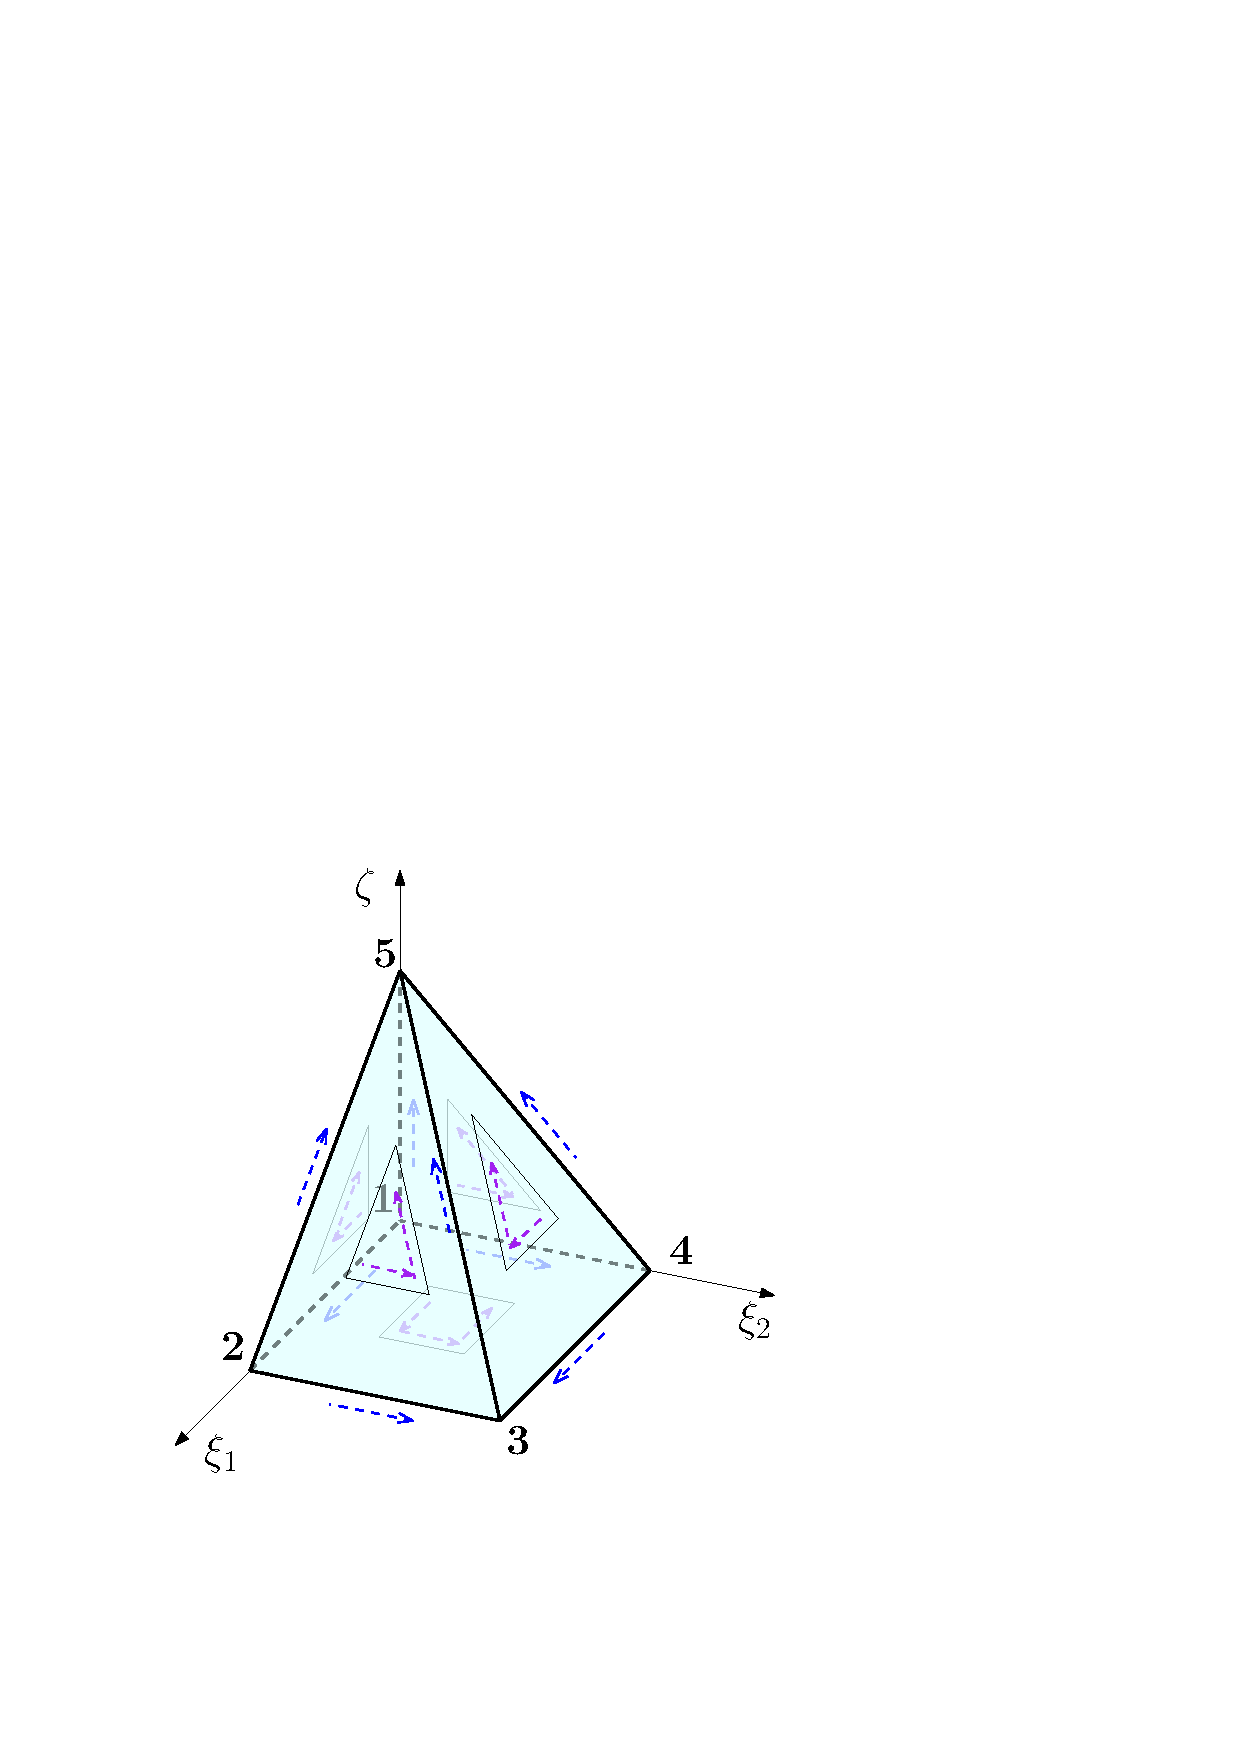
\includegraphics[scale=0.5]{./figures/MasterPyramidOrientations.pdf}
\caption{Master pyramid with numbered vertices \textit{and} local edge and face orientations.}
\label{fig:MasterPyramidOrientations}
\end{center}
\end{figure}

The predefined \textit{local} edge and face orientations for the pyramid are illustrated in Figure \ref{fig:MasterPyramidOrientations}.
They represent the $\oo=0$ case.
The task at hand is to find the associated \textit{locally ordered} tuples of affine coordinates representing those local orientations.
The key is being aware of the relationships between the vertices and the affine coordinates, which have been explained in detail at the beginning of this section. 
Hence, once \S\ref{sec:HexaOrientations}, \S\ref{sec:TetOrientations} and \S\ref{sec:PrismOrientations} are consulted, it should be clear how to construct the orientation embedded shape functions. 
Consult Appendix \ref{app:pyrappendix} if the reader wants to avoid computational instabilities for the $H(\mathrm{div})$ triangle face functions.

%Section 10
\newpage
\section{Conclusions}
\label{sec:Conclusions}

We have presented here a full systematic construction of hierarchical higher order shape functions for elements of ``all shapes'' (see Figure \ref{fig:elementsallshapes}) using the exact sequence logic.
Compatibility of the shape functions at the interelement boundaries is based on the idea of having a known fixed trace at the boundary which is extended (or lifted) to the rest of the element.
%In this work, this is called dimensional hierarchy.
Hence, the shape functions can be used in hybrid meshes containing elements of all shapes.
Furthermore, due to the properties of the discrete spaces, interpolation estimates are ensured in any hybrid master element mesh and for all energy spaces.

The unified construction is based at its core in considering tensor products of polynomials.
This has positive implications from the computational point of view, and could result in the successful implementation of fast integration techniques as described in Appendix \ref{app:Integration}.

Also, the shape functions allow the polynomial order $p$ to vary accross a given mesh. 
For example, the quadrilateral, hexahedron and prism shape functions are naturally anisotropic and can have different orders in each direction.
More so, each edge and face in the mesh can have their own order $p$, independent of the order of the neighboring edges, faces and interiors in the mesh.
Hence, techniques that exploit the use of local $p$ adaptivity can be implemented using these shape functions.

As polynomial building blocks, Legendre and Jacobi polynomials are used in this work.
Our results show that the recursive formulas presented in this document to implement those polynomials seem to be the most accurate in comparison to other recursive formulas. 
The choices of Jacobi and Legendre polynomials are known to have extremely good sparsity and conditioning properties for typical projection problems \citep{Beuchler_Pillwein_Schoeberl_Zaglmayr_12}.
However, there is flexibility in this choice of polynomials, and it might be worth investigating if there are applications where different choices provide useful advantages (see Appendix \ref{app:GeneratingFamilies}).

All constructions are written in terms of affine coordinates and their gradient.
Indeed, the shape functions are valid for any (typical) master element geometry, provided the affine coordinates are computed.
We hope this has convinced the reader that the direct use of affine coordinates for \textit{all} elements (not just simplices) is the ideal approach, and that it motivates other researchers to also communicate in those general terms.
The polynomials we chose are \textit{shifted} to have the domain $(0,1)$ instead of the typical $(-1,1)$.
We claim this is the natural choice for construction of shape functions, since all affine cordinates have range $[0,1]$ and affine coordinates are \textit{the} natural inputs for the polynomials.
Hence, we encourage the implementation of the polynomials in the shifted domain.
The concept of polynomial homogenization was introduced and heavily used.
It is a particular form of scaling which is closely related to affine coordinates, and is a tool that provides natural extensions.
In fact, homogenization provides some level of geometrical intuition, since the projected affine coordinates arise naturally through this process.
Theoretically it is also a convenient tool since it results in homogeneous polynomials, which have many desirable properties.

Moreover, only \textit{eight} ancillary operators effectively generate all shape functions.
These ancillary operators are coordinate free, in the sense that the form of the operators is invariant with respect to any transformation. 
This is important, because it allows to transform nonlinearly to other geometries.
Hence, it suffices to compute the affine coordinates and their gradient in that deformed space.
Then, the shape functions resulting from the substitution of the deformed affine coordinates will precisely be the well defined pullback of the original shape functions.
This has both theoretical and practical implications.
For example, curved physical elements are deformations of the master element domains. 
%For example, instead of integrating over a ``difficult'' domain, one can transform to the cube and integrate there (with suitable weights).
This has the potential to result in more efficient computations when integrating (see Appendix \ref{app:Integration} for the basics of integration).

For the face and edge shape functions, the logic of projecting, evaluating and blending is used consistently for all elements and all energy spaces.
This provides a firm geometrical intuition of the expressions and formulas for the shape functions, which we hope the reader will appreciate.

Additionally, the shape functions can be converted to orientation embedded shape functions via only \textit{three} local-to-global permutation functions (one for edges, one for triangle faces, and one for quadrilateral faces).
These orientation embedded shape functions are extremely practical in many applications, especially in the implementation of constrained nodes in $hp$ methods.

All the characteristics above prove to be vital in the implementation of a code.
Indeed, the number of important routines which are called repeatedly is very small, and this minimizes the sources of errors, while allowing a very focused optimization of the implementation.
A complete Fortran 90 code supplements this document.\footnote{See the ESEAS library available at https://github.com/libESEAS/ESEAS.}
It provides an excellent guidance if the reader is ever interested in implementing this construction.  
The code has been tested thoroughly by numerically checking polynomial reproducibility and exact sequence properties.
This is described in Appendix \ref{app:verification}.
The shape functions for all elements and all spaces are conveniently summarized in Appendix \ref{app:ShapeFunctionTable}.
%This should provide a helpful company for the reader when implementing them numerically.
%Due to the properties of the discrete spaces, interpolation estimates are ensured in any hybrid master element mesh.
%Thoughout the construction there is a consistent use of the logic of projecting, evaluating and blending.

%For simplices (segment, triangle, tetrahedron), our construction is hierarchical in polynomial order $p$. For Cartesian product elements, we conform to the tensor product structure (and numbering). This facilitates implementation of hanging nodes.

Lastly, special attention is given to the successful construction of the pyramid shape functions, which is rare in the literature.
A thorough geometric intuition for the pyramid was described, and the 3D pyramid affine-related coordinates were defined and analyzed.
The set of exact sequence spaces were taken from \citet{Nigam_Phillips_11}, and they are consistent with the fundamental first order elements described by \citet{Hiptmair99}.
We believe it to be the first time that an arbitrary high order construction of $H(\mathrm{div})$ shape functions has been implemented whilst respecting those lower order spaces (there have been others where either the lower order spaces have been larger, or simply different).
This may prove to be very valuable to other researchers even if only for comparison purposes.
For the pyramid, it might be possible to investigate better choices of polynomials for the bubbles, as this may provide better conditioning and sparsity properties.

To finalize, we hope this construction has been useful in its methoodology and that it motivates further research in this very rich area.

%Moreover, it is also interesting to investigate the spaces of bubbles in more detail, since only by modifying these it might be possible to construct smaller exact sequence discrete spaces.
%As explained in \S\ref{sec:Introduction}, the shape functions are organized into groups corresponding to different topological entities. These are the element node: vertices, edges, faces, and interiors. This naturally allows for anisotropic orders (spaces) for nodes in Cartesian product elements. The resulting {\em elements of variable order} form a foundation for the $p$ and $hp$ finite element method.

%This work is supplemented with a complete FORTRAN 90 package defining all of the shape functions presented here. The reader may also exploit Tables~\ref{app:ShapeFunctionTable} to reference all the shape functions presented in this document.
%
%Although the total number of different shape functions seems to be large, we signal that we have actually required very few unique functions. The simplicity and elegance is reflected in the length and complexity of the code.

%Our methodology, sometimes referred to throughout the document as ``projecting, evaluating, and blending,'' is designed in a general way to apply to all elements discussed and all spaces in the exact sequence. Moreover, this approach does not rely upon any particular geometry for the master elements. It is applicable for {\em all} geometries of the elements of ``all shapes.''%Although we have made a specific choice in our element geometries and exploited this choice, the reader could easily modify the geometry and our methodology would still apply.

%We have demonstrated the utility of the affine coordinate approach to shape function construction. Specifically this is true in regard to orientation embedded shape functions. Readers not interested in orientation embedded constructions can obviously still use our construction with the orientation $o=0$.

% \subsection{Future Directions}
%Looking forward, we note that our construction of tensor product shape functions (Cartesian product elements) often makes use of blending functions of the first order. This choice has been made to ensure a maximally anisotropic set of shape functions. It is well known \textit{cite} that using higher order blending functions results in better conditioning. The user could easily augment the blending functions we have chosen in order to provide this feature.

%Our initial choice of basis polynomials discussed in Section~\ref{sec:Notation} (Legendre and Jacobi), while adequate for our purposes, may be enhanced by using other polynomial bases. Our choice was motivated by the use of Lagrange and Jacobi polynomials in existing literature. However, a careful analysis of other candidate polynomial spaces may yield other shape functions giving better conditioning as well as sparsity properties. At this time, we know of no strictly better choices.

%%%%%%%%%%%%%%%%%%%%%%%%%%%%%%%%%%%%%%%%%%%%%%%%%%%%%%%%%%%%%%%%%%%%%%%%%%%%%%%
% Throughout the text, we do not separate $H(\text{curl})$ functions into those with nonzero and zero curl (the gradients of $H^1$). Similarly, we do not separate $H(\text{div})$ functions into those with nonzero and zero divergence (the curls of $H(\text{curl})$).% This is because of a ``head on'' conflict of such a separation with tensor product constructions which is essential for our FE codes, in particular implementation of hanging nodes. Such a separation is essential for the construction of iterative solvers for $H(\text{curl})$ and $H(\text{div})$ problems so in that sense, our construction is perhaps a step backwards.
% However, at the bubble level, such a Helmholtz decomposition may potentially be implemented in the future. {\color{red} $\longleftarrow$ Federico has done this for the pyramid and we believe that we can do it in general.}

\paragraph{Acknowledgements.}
The work of Fuentes, Keith, Demkowicz and Nagaraj was supported with grants by AFOSR (FA9550-12-1-0484), NSF (DMS-1418822) and Sandia National Laboratories (1536119).

%References
\newpage
\phantomsection%For hyperref
\addcontentsline{toc}{section}{References}
\bibliographystyle{kbib}
\bibliography{main}

%Appendices
\appendix
%Appendix A
\newpage
\pagenumbering{arabic}% resets counter to 1
\renewcommand*{\thepage}{\thesection-\arabic{page}}%Custom numbering
\section{Polynomial Families}
\label{app:GeneratingFamilies}

Let $\mathcal{P}^i(x)=\mathrm{span}\{x^j:j=0,\ldots,i\}$ be the polynomials of order $i$, and $\mathcal{F}_p=\{P_i:i=0,\ldots,p-1\}$ and $\mathcal{F}_p^\alpha=\{P_j^\alpha:j=0,\ldots,p-1\}$ be sets of polynomials with domain $x\in[0,1]$. 
The families $\mathcal{F}_p$ and $\mathcal{F}_p^\alpha$ should satisfy that $\mathrm{span}(\mathcal{F}_p)=\mathrm{span}(\mathcal{F}_p^\alpha)=\mathcal{P}^{p-1}(x)$, $P_i\in\mathcal{P}^i(x)$ and $P_j^\alpha\in\mathcal{P}^j(x)$.
Moreover, the family $\mathcal{F}_p$ should satisfy the zero average property, $\int_0^1 P_i(x)\,\mathrm{d}x=0$, for all $i\geq1$.

These sets of conditions are very easy to satisfy. 
For example consider any sequence of polynomials of increasing order, say $1,x,x^2,x^3,\ldots,x^{p-1}$.
Then it is only a matter of adding a suitable constant to all polynomials of order $i\geq1$ such that their integral is $0$.
For example, $1,x,x^2,x^3,\ldots,x^p$ becomes $1,x-\frac{1}{2},x^2-\frac{1}{3},\ldots,x^{p-1}-\frac{1}{p}$, and this latter one is already a suitable family $\mathcal{F}_p$.

The elements of $\mathcal{F}_p$ and $\mathcal{F}_p^\alpha$ are thought of being elements of $L^2$, even though they are infinitely differentiable as polynomials.
Indeed, it is often desirable that the elements of $\mathcal{F}_p$ and $\mathcal{F}_p^\alpha$ satisfy certain properties in the $L^2$ (or weighted $L^2$) inner product, since they can result in considerably sparser finite element matrices.
In fact, orthogonality of the $P_i$, is generally seeked.
If there is no weight, orthogonality of the $P_i$ is attained uniquely (up to a constant) by the Legendre polynomials, and this is why they are the typical choice.
Meanwhile, the family $\mathcal{F}_p^\alpha$ can also be chosen wisely by taking into account a weighted $L^2$ space relevant to the triangle element.
If the $P_i$ are Legendre polynomials, the natural choice for the $P_j^\alpha$ is to be Jacobi polynomials with certain weights.

Now, define the polynomials $L_{i}\in\mathcal{P}^{i}(x)$ and $L_{j}^\alpha\in\mathcal{P}^{j}(x)$ from the $P_{i-1}\in\mathcal{F}_p$ and $P_{j-1}^\alpha\in\mathcal{F}_p^\alpha$ as
\begin{equation}
    L_{i}(x)=\int_0^x P_{i-1}(\tilde{x})\,\mathrm{d}\tilde{x}\,,\qquad\qquad 
    	L_{j}^\alpha(x)=\int_0^x P_{j-1}^\alpha(\tilde{x})\,\mathrm{d}\tilde{x}\,,
\end{equation}
for $i=2,\ldots,p$ and $j=1,\ldots,p$.
Clearly, it follows that $\mathcal{P}^{p}(x)=\mathcal{P}^1(x)\cup\{L_i:i=2,\ldots,p\}$ and $\mathcal{P}^{p}(x)=\mathcal{P}^0(x)\cup\{L_j^\alpha:j=1,\ldots,p\}$.
By construction, the $L_i$ and $L_j^\alpha$ are elements of $H^1$ and as a result their pointwise evaluation exists. 
In fact, due to the zero average property, 
\begin{equation}
	\begin{alignedat}{3}
		L_i(0)&=L_i(1)=0\,,\qquad\qquad&&\text{for }i\geq2\,,\\
		L_j^\alpha(0)&=0\,,\qquad\qquad&&\text{for }i\geq1\,.
	\end{alignedat}
	\label{eq:AppLiLjVanishingProperties}
\end{equation}

%\begin{equation}
%    \begin{alignedat}{3}
%        L_i(0)&=0\quad i=1,\ldots,p\,\,\,\Rightarrow\,\,\,
%            L_i(x)=xf_{i-1}(x)\,\,\, && \text{with }f_{i-1}\in\mathcal{P}^{i-1}(x)\quad i=1,\ldots,p\\
%        L_i(1)&=0\quad i=2,\ldots,p\,\,\,\Rightarrow\,\,\,
%            L_i(x)=x(1-x)f_{i-2}(x)\,\,\, && \text{with }f_{i-2}\in\mathcal{P}^{i-2}(x)\quad i=2,\ldots,p\,.
%    \end{alignedat}
%\end{equation}

% %I use the properties above. I was thinking you can go on defining scaling, then the partial derivatives. Intorduce R_i before even starting on Legendre and use your general formula you showed this morning. Afterwards in another subsection you introduce Legendre with all the associated formulas and recursions and analogously with Jacobi. This subsection covers the main properties that the families of polynomials should satisfy.

Now, apply the definition of scaling given in \eqref{eq:scaledpolyomials} to the polynomials, yielding $P_i(x;t)$, $P_j^\alpha(x;t)$, $L_i(x;t)$ and $L_j^\alpha(x;t)$, where $x\in[0,t]$.
In particular, note that
\begin{equation}
	L_{i+1}(x;t)=t^{i+1}L_{i+1}\Big(\frac{x}{t}\Big)=t^{i+1}\int_0^{\frac{x}{t}} P_{i}(\tilde{x})\,\mathrm{d}\tilde{x}
		=t^{i}\int_0^{x} P_{i}\Big(\frac{\tilde{y}}{t}\Big)\,\mathrm{d}\tilde{y}\,.
\end{equation}
Since the scaled polynomials are now bivariate polynomials in $(x,t)$, it is useful to find the derivatives in both of these variables.
Using the latter equality above,
\begin{equation}
	\frac{\partial}{\partial x}L_{i+1}(x;t)=t^iP_i\Big(\frac{x}{t}\Big)=P_i(x;t)\,.
\end{equation}
Meanwhile, using the other equality, it follows
\begin{equation}
	\frac{\partial}{\partial t}L_{i+1}(x;t)
		=(i+1)t^iL_{i+1}\Big(\frac{x}{t}\Big)+t^{i+1}P_{i}\Big(\frac{x}{t}\Big)\Big(\frac{-x}{t^2}\Big)
			=t^i\Big((i+1)L_{i+1}\Big(\frac{x}{t}\Big)-\Big(\frac{x}{t}\Big)P_{i}\Big(\frac{x}{t}\Big)\Big)\,.
\end{equation}
This suggests the definition
\begin{equation}
	R_i(x)=(i+1)L_{i+1}(x) - xP_i(x)\,,
	\label{eq:R_i_eq1}
\end{equation}
for $i\geq1$.
Using the leading order term of $P_i$, the reader may observe that $R_i$ is an order $i$ polynomial (\textit{not} order $i+1$), so the indexing with $i$ makes sense.
More importantly,
\begin{equation}
	\frac{\partial}{\partial t}L_{i+1}(x;t)
			=t^i\Big((i+1)L_{i+1}\Big(\frac{x}{t}\Big)-\Big(\frac{x}{t}\Big)P_{i}\Big(\frac{x}{t}\Big)\Big)
				=R_{i}(x;t)\,.
\end{equation}
Exactly the same analysis applies to the $L_{j+1}^\alpha$, meaning that
\begin{equation}
	\frac{\partial}{\partial x}L_{j+1}\alpha(x;t)=P_j^\alpha(x;t)\,,\qquad\qquad
		\frac{\partial}{\partial x}L_{j+1}^\alpha(x;t)=R_j^\alpha(x;t)\,,
\end{equation}
for $j\geq0$, and where
\begin{equation}
	R_j^\alpha(x)=(j+1)L_{j+1}^\alpha(x) - xP_j^\alpha(x)\,.
\end{equation}

As observed, all these properties are deduced at a very general level, and apply to any families $\mathcal{F}_p$ and $\mathcal{F}_p^\alpha$ satisfying the simple set of properties mentioned initially.
To conclude, it follows all the results deduced throughout the document still hold for these more general polynomial families, including the vanishing properties, the ancillary function properties, etc.
Hence, the reader may decide to change these families if desired.
This could potentially provide better sparsity properties depending on the problem.
Nevertheless, be aware that for the classical Laplace problem (and many related sets of problems), the ideal polynomial families are the Legendre and Jacobi polynomials, which are used throughout this document and are conveniently defined through recursive formulas.

%By definion,
%\begin{equation}
%L_{i+1}(x;t) = \int_0^x P_i(\tilde{x};t) d\tilde{x}=\int_0^x P_i\left(\frac{\tilde{x}}{t}\right)t^i d\tilde{x}
%=t^{i+1}\int_0^\frac{x}{t} P_i\left(\tilde{x}\right) d\tilde{x}\,,
%\end{equation}
%and so
%\begin{equation}
%\frac{\ptl}{\ptl t} L_{i+1}(x;t) = (i+1) t^i\int_0^\frac{x}{t} P_i\left(\tilde{x}\right) d\tilde{x} + t^{i+1}\left(-\frac{x}{t^2}\right)P_i\left(\frac{x}{t}\right)\,.
%\end{equation}
%This gives us the useful equation
%\begin{equation}
%t \frac{\ptl}{\ptl t} L_{i+1}(x;t) = (i+1)L_{i+1}(x;t) - xP_i(x;t)\,.
%\end{equation}
%With the definiton,
%\begin{equation}
%R_i(x) := (i+1)L_{i+1}(x) - xP_i(x)\,,
%\label{eq:R_i_eq1}
%\end{equation}
%we observe that
%\begin{equation}
%\frac{\ptl}{\ptl t} L_{i+1}(x;t) = R_i(x;t)\,.
%\end{equation}



%Appendix B
\newpage
\pagenumbering{arabic}% resets counter to 1
\renewcommand*{\thepage}{\thesection-\arabic{page}}%Custom numbering
\section{Pyramid Supplement}
\label{app:pyrappendix}

\begin{figure}[!ht]
\begin{center}
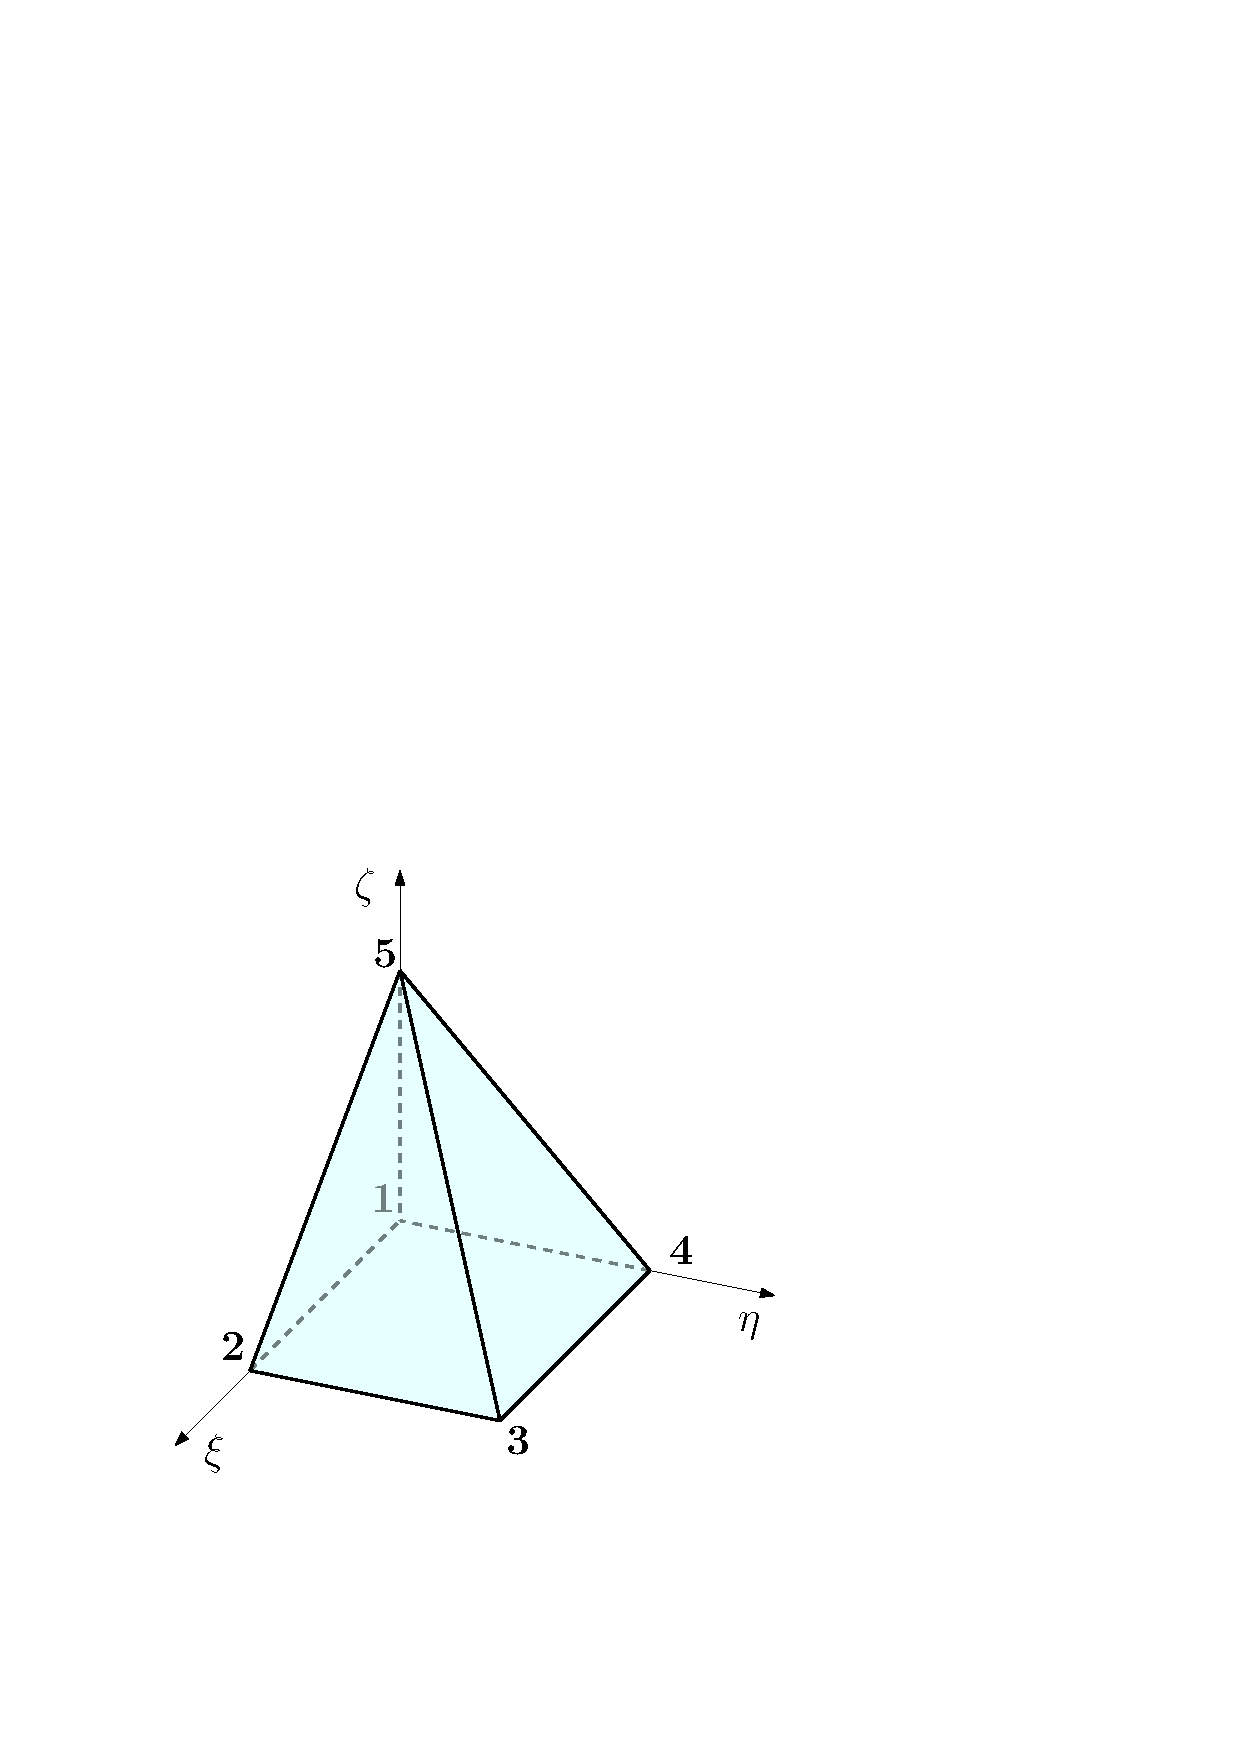
\includegraphics[scale=0.5]{./figures/MasterPyramidAppendix.pdf}
\caption{Master pyramid with numbered vertices.}
\label{fig:MasterPyramidAppendix}
\end{center}
\end{figure}

The master pyramid is shown in Figure \ref{fig:MasterPyramidAppendix} in the $(\xi,\eta,\zeta)$ space (\textit{not} the $(\xi_1,\xi_2,\zeta)$ space).
More specifically, the definition is $\Omega=\{(\xi,\eta,\zeta)\in\R^3:\xi>0,\eta>0,\zeta>0,\xi+\zeta<1,\eta+\zeta<1\}$.

This supplement provides the proofs that the pyramid shape functions proposed in \S\ref{sec:Pyramid} are in the finite element spaces  defined in the fundamental work by \citet{Nigam_Phillips_11}.
%These discrete spaces are defined in the fundamental work by \citet{Nigam_Phillips_11}.
Recall from \eqref{eq:pyramidsequence} that the discrete spaces forming the exact sequence are $\mathcal{U}^{(m),p}$ for $m=0,1,2,3$, where $m$ stands for the differential $m$-forms lying in each space.
The spaces $\mathcal{U}^{(m),p}$ are defined as
\begin{equation}
	\mathcal{U}^{(m),p}=\mathcal{V}^{(m),p}\cap\Gamma^{(m),p}\,,
\end{equation}
where the spaces $\mathcal{V}^{(m),p}$ are called the \textit{underlying spaces}, and the spaces $\Gamma^{(m),p}$ are called the \textit{compatibility spaces}.
These two families of spaces will be defined next.

First, note that the compatibility spaces ensure the elements in $\mathcal{U}^{(m),p}$ are compatible at the level of spaces with the other elements.
Indeed, they consist of those functions having their face traces lying on the appropriate 2D quadrilateral and triangle spaces in \eqref{eq:QuadES} and \eqref{eq:EStriangle} respectively.
More specifically, let $\mathrm{tr}_\Tri^{(m)}$ and $\mathrm{tr}_\square^{(m)}$ be the trace of the differential $m$-forms over the four pyramid triangle faces and the pyramid quadrilateral face respectively.
Recall that for $m=0$ the trace is the value of the function itself, for $m=1$ the trace is the 2D tangential component, while for $m=2$ the trace is the normal component.
With this in mind, the compatibility spaces are,\footnote{Note that in \eqref{eq:Pyramidcompatilibityspaces}, the very special property that $\mathcal{P}^p$, $\mathcal{N}^p$ and $\mathcal{RT}^p$ are affine invariant is used. If the spaces were different, one would need to take the 2D pullback of each triangle trace to the master triangle. The same holds for the quadrilateral trace, where in this case it is exploited that the quadrilateral face is the master quadrilateral and no transformation is needed.}
\begin{equation}
\begin{aligned}
	\Gamma^{(0),p}&=\{\phi\in H^1:\mathrm{tr}_\Tri^{(0)}(\phi)\in\mathrm{tr}_\Tri^{(0)}(\mathcal{P}^p(\xi,\eta,\zeta)),\,\,
		\mathrm{tr}_\square^{(0)}(\phi)\in\mathcal{Q}^{p,p}(\xi,\eta)\}\,,\\
%			\mathrm{tr}_\square^{(0)}(\mathcal{Q}^{p,p,p})\}\,,\\
	\Gamma^{(1),p}&=\{E\in H(\mathrm{curl}):\mathrm{tr}_\Tri^{(1)}(E)\in\mathrm{tr}_\Tri^{(1)}(\mathcal{N}^p(\xi,\eta,\zeta)),\,\,
		\mathrm{tr}_\square^{(1)}(E)\in\mathcal{Q}^{p-1,p}(\xi,\eta)\!\times\!\mathcal{Q}^{p,p-1}(\xi,\eta)\}\,,\\
%			\mathrm{tr}_\square^{(1)}(\mathcal{Q}^{p-1,p,p}\times\mathcal{Q}^{p,p-1,p}\times\mathcal{Q}^{p,p,p-1})\}\,,\\
	\Gamma^{(2),p}&=\{V\in H(\mathrm{div}):\mathrm{tr}_\Tri^{(2)}(V)\in\mathrm{tr}_\Tri^{(2)}(\mathcal{RT}^p(\xi,\eta,\zeta)),\,\,
		\mathrm{tr}_\square^{(2)}(V)\in\mathcal{Q}^{p-1,p-1}(\xi,\eta)\}\,,\\
%			\mathrm{tr}_\square^{(2)}(\mathcal{Q}^{p,p-1,p-1}\times\mathcal{Q}^{p-1,p,p-1}\times\mathcal{Q}^{p-1,p-1,p})\}\,,\\
	\Gamma^{(3),p}&=\{\psi\in L^2\}\,.
\end{aligned}
\label{eq:Pyramidcompatilibityspaces}
\end{equation}
%Note that $\mathcal{Q}^{p,p}(\xi,\eta)=\mathrm{tr}_\square^{(0)}(\mathcal{Q}^{p,p,p}(\xi,\eta,\zeta))$ and similarly with $m=1,2$.

Fortunately, at the level of shape functions, dealing with the compatibility spaces is not as intimidating as it might look.
All that is required is that the shape functions satisfy the dimensional hierarchy, so that their nonzero face traces correspond to the lower dimensional shape functions, which are known to lie in the correct space.
Therefore, if a shape function satisfies the required trace properties, it \textit{automatically} belongs to the appropriate compatibility space.

The main difficulty lies in showing that the shape functions belong to the underlying spaces $\mathcal{V}^{(m),p}$.
In fact, these spaces are not nicely defined directly on the master pyramid.
For this reason, it is more convenient to define them on a deformed space where the symmetries are more evident, and then use the inverse pullback to the master pyramid.
This process is explained in what follows.

%Instead of defining them directly on the master pyramid, the spaces are defined on a deformed space where the symmetries are more evident, and then mapped back to the master pyramid.
%This is a typical approach.
%The deformed space is usually chosen as a cube, but \citet{Nigam_Phillips_11} chose it to be an \textit{infinite pyramid}, which is defined as $\Omega_\infty=\{(x,y,z)\in\R^3:0<x<1,0<y<1,z>0\}$.
%The necessary concepts to define the spaces are presented in what follows.
%%before presenting the definition, some preliminary concepts are required first.
%%These discrete spaces are not defined yet, and defining them will be the next mission.

\begin{figure}[!ht]
\begin{center}
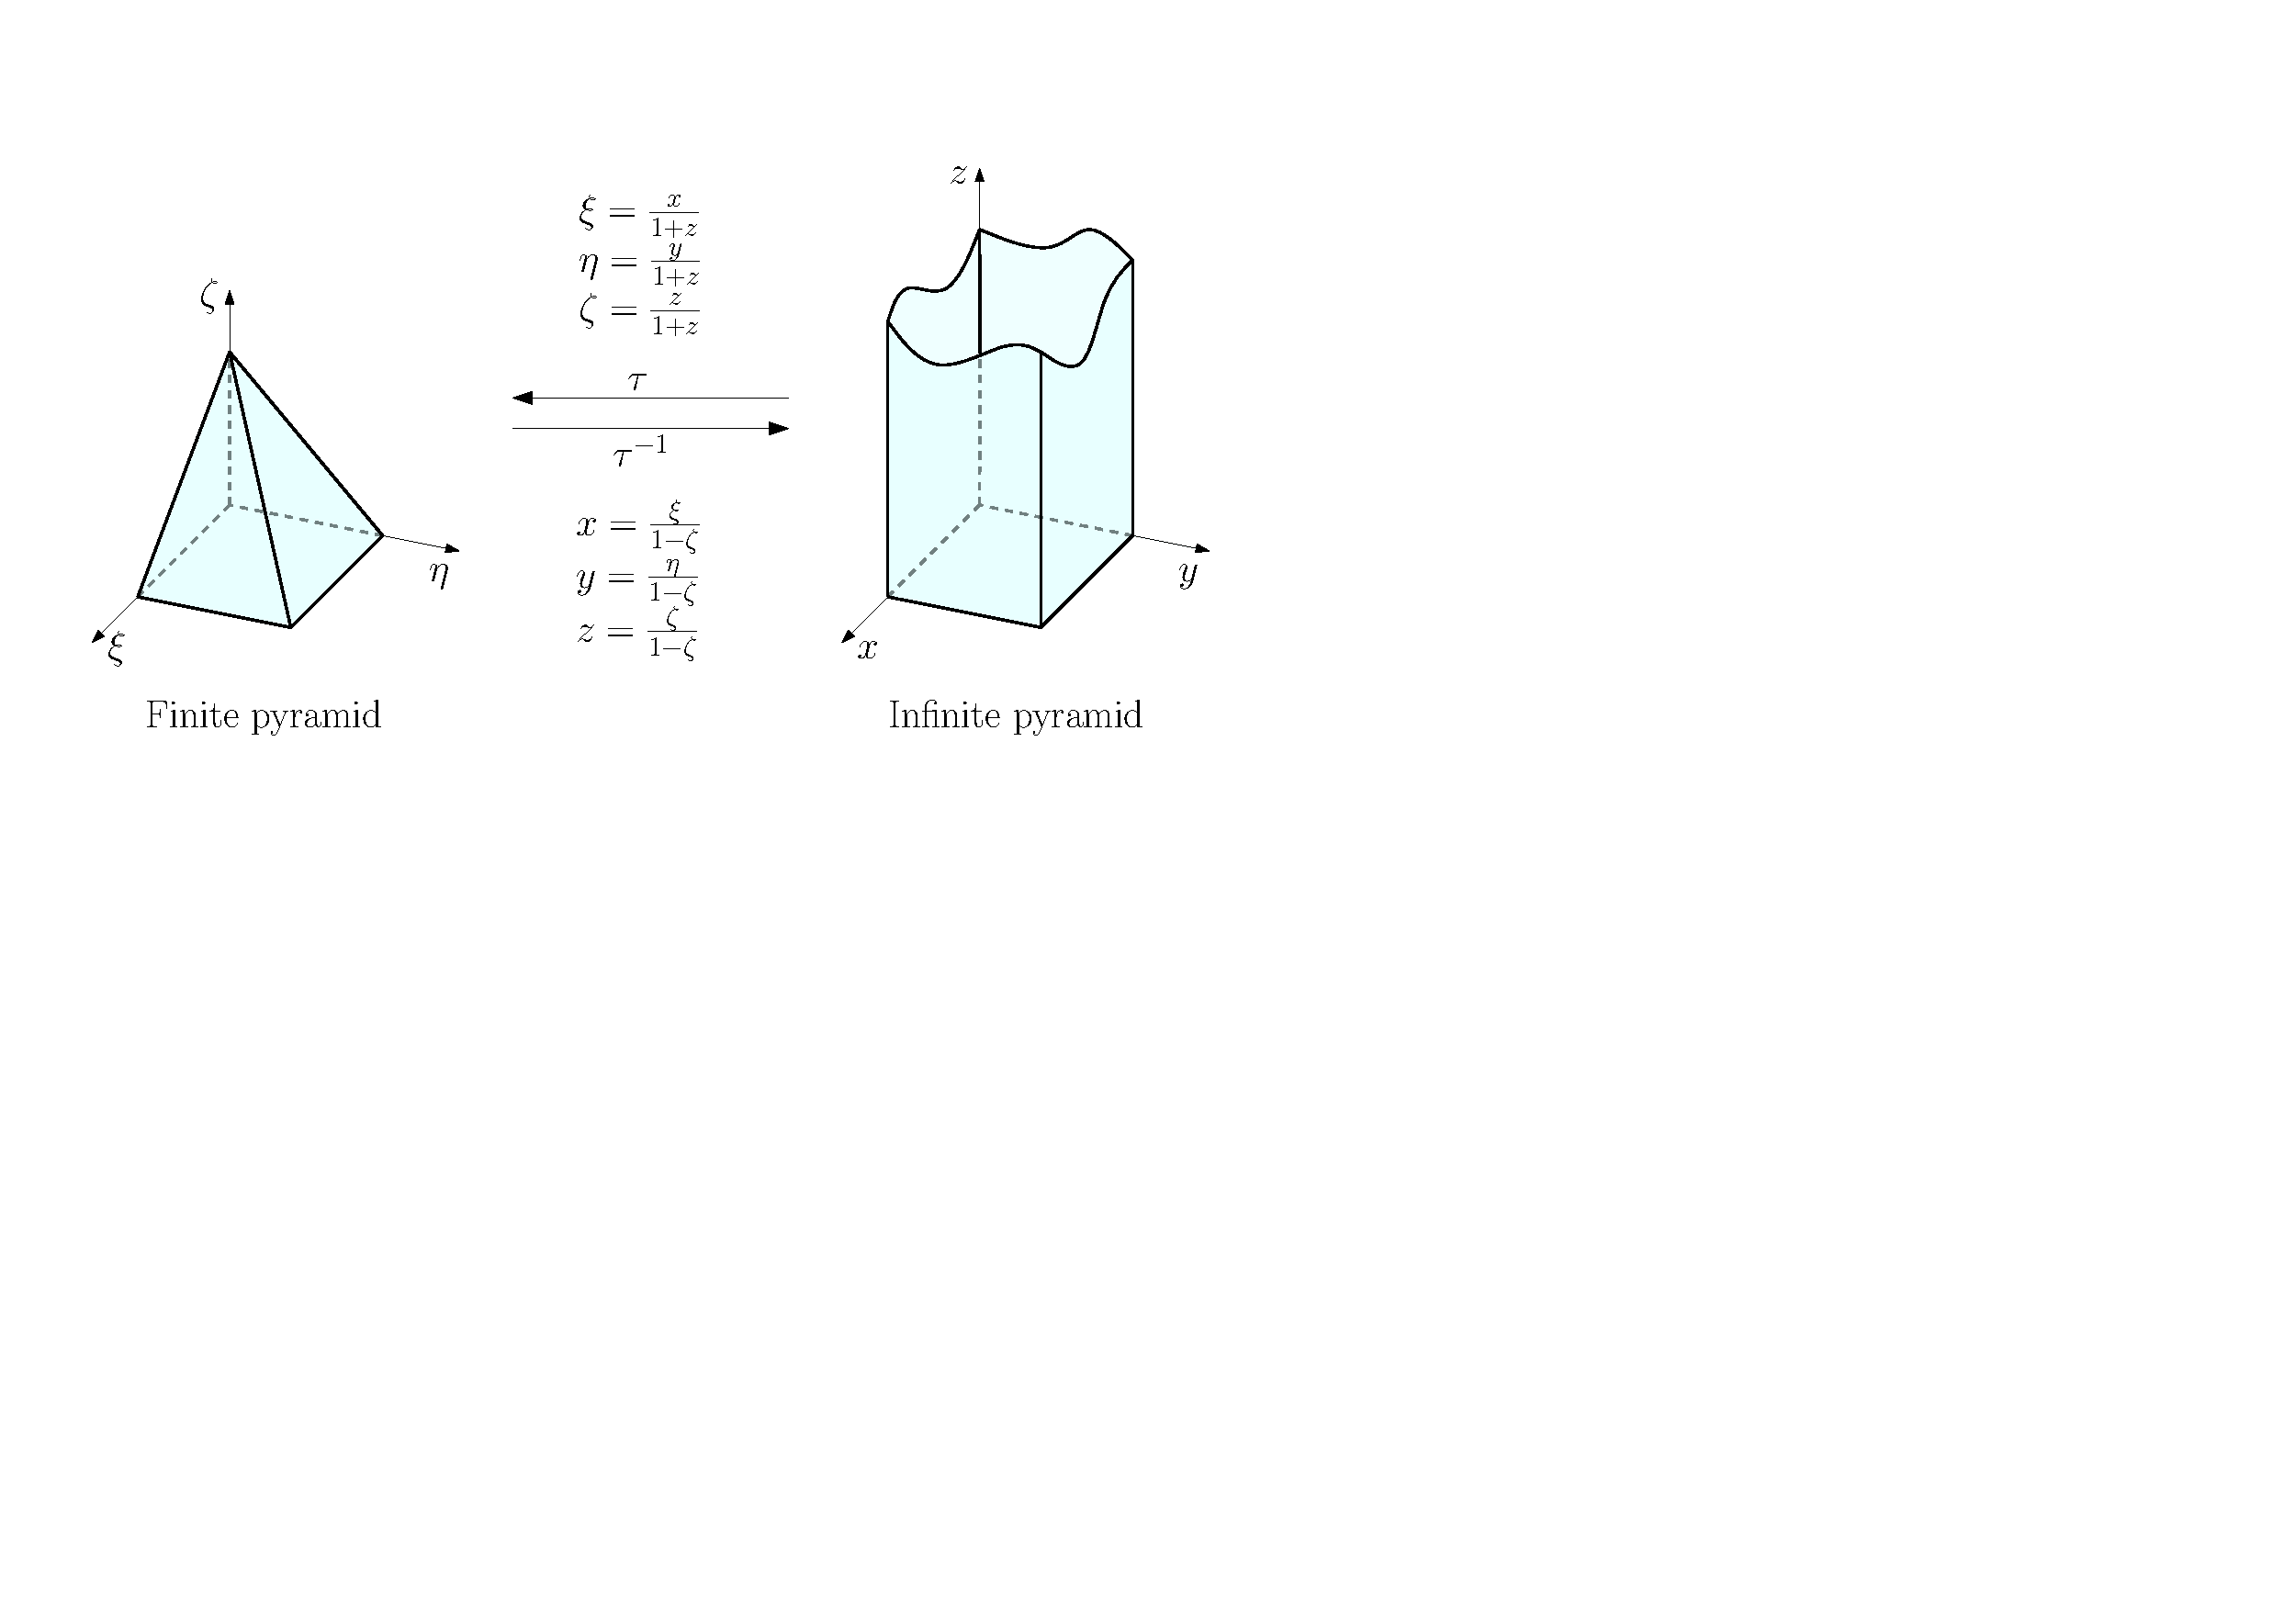
\includegraphics[scale=0.5]{./figures/PyramidSingleTransform.pdf}
\caption{Transformation from the infinite pyramid to the master pyramid.}
\label{fig:PyramidSingleTransform}
\end{center}
\end{figure}

The deformed space is usually chosen as a cube, but \citet{Nigam_Phillips_11} chose it to be an \textit{infinite pyramid}, which is defined as $\Omega_\infty=\{(x,y,z)\in\R^3:0<x<1,0<y<1,z>0\}$.
The first step is to consider the transformation $\tau:\Omega_\infty\rightarrow\Omega$ from the intinite pyramid $\Omega_\infty$ to the pyramid $\Omega$, which is given by the component equations,
\begin{equation}
	\xi=\frac{x}{1+z},\quad\qquad\eta=\frac{y}{1+z},\quad\qquad\zeta=\frac{z}{1+z}\,.
\end{equation}
Clearly, $\tau$ is a diffeomorphism between these open sets (\textit{not} when including the boundary).
The inverse $\tau^{-1}:\Omega\rightarrow\Omega_\infty$ is given by the component equations,
\begin{equation}
	x=\frac{\xi}{1-\zeta},\quad\qquad y=\frac{\eta}{1-\zeta},\quad\qquad z=\frac{\zeta}{1-\zeta}\,.
\end{equation}
The transformation is depicted in Figure \ref{fig:PyramidSingleTransform}.
Take note of the following useful expressions resulting from this transformation,
\begin{equation*}
	1-x=\frac{1-\xi-\zeta}{1-\zeta},\quad\quad 1-y=\frac{1-\eta-\zeta}{1-\zeta},\quad\quad
	1+z=\frac{1}{1-\zeta},\quad\quad \frac{1}{1+z}=1-\zeta\,.
\end{equation*}

Next consider the following isomorphic mappings,
\begin{equation}
\begin{aligned}
	\tau^{-*,(m)}:&\mathcal{V}_\infty^{(m),p}\longrightarrow\mathcal{V}^{(m),p}=\tau^{-*,(m)}(\mathcal{V}_\infty^{(m),p})\,,\\
		\tau^{*,(m)}:&\mathcal{V}^{(m),p}\longrightarrow\mathcal{V}_\infty^{(m),p}\,,
\end{aligned}
\end{equation}
where $\tau^{-*,(m)}$ and $\tau^{*,(m)}$ are the inverse pullback and pullback mappings induced by $\tau$.
Since the spaces $\mathcal{V}^{(m),p}$ and $\mathcal{V}_\infty^{(m),p}$ are isomorphic, it is mathematically irrelevant which of the two spaces is actually defined, since the other space can be determined through the corresponfing pullback mapping.
However, sometimes there are practical reasons to explicitly define one set of spaces over the other.
Indeed, it is more opportune to define the deformed underlying spaces $\mathcal{V}_\infty^{(m),p}$, which are\footnote{Note there is misprint in \citet{Nigam_Phillips_11} in (3.8) when presenting the equivalent characterization of $\mathcal{V}_\infty^{(1),p}$. The definition here corrects that, and is consistent with the calculations in \S3.3 of \citet{Nigam_Phillips_11}.}
\begin{equation}
\begin{aligned}
	\mathcal{V}_\infty^{(0),p}&=\{\phi\!\in\!\mathcal{Q}_p^{p,p,p}:
		\nabla\phi\!\in\!\mathcal{Q}_p^{p-1,p,p-1}\!\times\!\mathcal{Q}_p^{p,p-1,p-1}\!\times\!\mathcal{Q}_{p+1}^{p,p,p-1}\}\,,\\
	\mathcal{V}_\infty^{(1),p}&=\{E\!\in\!
		\mathcal{Q}_{p+1}^{p-1,p,p}\!\times\!\mathcal{Q}_{p+1}^{p,p-1,p}\!\times\!\mathcal{Q}_{p+1}^{p,p,p-1}:
			\nabla\!\times\! E\!\in\!
				\mathcal{Q}_{p+2}^{p,p-1,p-1}\!\times\!\mathcal{Q}_{p+2}^{p-1,p,p-1}\!\times\!\mathcal{Q}_{p+1}^{p-1,p-1,p-1}\}\,,\\
	\mathcal{V}_\infty^{(2),p}&=\{V\!\in\!
		\mathcal{Q}_{p+2}^{p,p-1,p-1}\!\times\!\mathcal{Q}_{p+2}^{p-1,p,p-1}\!\times\!\mathcal{Q}_{p+2}^{p-1,p-1,p}:
			\nabla\cdot V\!\in\!\mathcal{Q}_{p+3}^{p-1,p-1,p-1}\}\,,\\
	\mathcal{V}_\infty^{(3),p}&=\{\psi\!\in\!\mathcal{Q}_{p+3}^{p-1,p-1,p-1}\}\,,
\end{aligned}
\end{equation}
where $\mathcal{Q}_{n}^{p,q,r}=\mathcal{Q}_{n}^{p,q,r}(x,y,z)$ are the $n$-weighted tensor polynomial spaces. 
They are defined as
\begin{equation}
	\mathcal{Q}_{n}^{p,q,r}(x,y,z)
		=\Big\{\frac{\psi(x,y,z)}{(1+z)^n}:\psi(x,y,z)\in\mathcal{Q}^{p,q,r}(x,y,z)\Big\}\,.
\end{equation}
Note the useful inclusion $\mathcal{Q}_{n}^{p,q,r}\subseteq\mathcal{Q}_{n+1}^{p,q,r+1}$ which holds for these rational polynomial spaces.

Lastly, note that the pullbacks $\tau^{*,(m)}$ take different forms depending on $m$.
Indeed, if $J_\tau$ is the Jacobian of the transformation $\tau$, the pullbacks are,
\begin{equation}
\begin{alignedat}{3}
	\tau^{*,(0)}\phi&=\phi\circ\tau\,,\quad&&\phi\in H^1\,,\\
	\tau^{*,(1)}E&=J_\tau^{\T}(E\circ\tau)\,,\quad && E\in H(\mathrm{curl})\,,\\
	\tau^{*,(2)}V&=\det(J_\tau)J_\tau^{-1}(V\circ\tau)\,,\quad && V\in H(\mathrm{div})\,,\\
	\tau^{*,(3)}\psi&=\det(J_\tau)(\psi\circ\tau)\,,\quad && \psi\in L^2\,.
\end{alignedat}
\label{eq:pullbacksgeneral}
\end{equation}
The same relations hold for the inverse pullbacks $\tau^{-*,(m)}$, but replacing $\tau$ by $\tau^{-1}$, $J_\tau$ by $J_{\tau^{-1}}$, and the domains by their isometrically isomorphic counterparts,\footnote{The spaces are iso\textit{metrically} isomorphic if the appropriate weights are added to the definition of the norm.} $H_\infty^1=\tau^{*,(0)}(H^1)$, $H(\mathrm{curl})_\infty=\tau^{*,(1)}(H(\mathrm{curl}))$, $H(\mathrm{div})_\infty=\tau^{*,(2)}(H(\mathrm{div}))$, and $L_\infty^2=\tau^{*,(3)}(L^2)$.
Even though they will be unnecessary, in the interest of completeness these pullback mappings are written explicitly below,
\begin{equation}
\begin{alignedat}{3}
	\tau^{*,(0)}\phi&=\phi\circ\tau\,,\quad
		&&\phi\in H^1\,,\\
	\tau^{*,(1)}E&=\frac{1}{(1+z)^2}\begin{pmatrix}1+z&0&0\\0&1+z&0\\-x&-y&1\end{pmatrix}(E\circ\tau)\,,\quad
		&& E\in H(\mathrm{curl})\,,\\
	\tau^{*,(2)}V&=\frac{1}{(1+z)^3}\begin{pmatrix}1&0&x\\0&1&y\\0&0&1+z\end{pmatrix}(V\circ\tau)\,,\quad
		&& V\in H(\mathrm{div})\,,\\
	\tau^{*,(3)}\psi&=\frac{1}{(1+z)^4}(\psi\circ\tau)\,,\quad
		&&\psi\in L^2\,.
\end{alignedat}
\label{eq:Pyramidpullbacks}
\end{equation}
The inverse pullbacks explicitly are,
\begin{equation}
\begin{alignedat}{3}
	\tau^{-*,(0)}\phi&=\phi\circ\tau^{-1}\,,\quad 
		&&\phi\in H_\infty^1\,,\\
	\tau^{-*,(1)}E&=\frac{1}{(1-\zeta)^2}\begin{pmatrix}1-\zeta&0&0\\0&1-\zeta&0\\\xi&\eta&1\end{pmatrix}(E\circ\tau^{-1})\,,\quad 
		&& E\in H(\mathrm{curl})_\infty\,,\\
	\tau^{-*,(2)}V&=\frac{1}{(1-\zeta)^3}\begin{pmatrix}1&0&-\xi\\0&1&-\eta\\0&0&1-\zeta\end{pmatrix}(V\circ\tau^{-1})\,,\quad 
		&& V\in H(\mathrm{div})_\infty\,,\\
	\tau^{-*,(3)}\psi&=\frac{1}{(1-\zeta)^4}(\psi\circ\tau^{-1})\,,\quad 
		&&\psi\in L_\infty^2\,.
\end{alignedat}
\label{eq:Pyramidinversepullbacks}
\end{equation}

To prove the shape functions defined in \S\ref{sec:Pyramid} are in the underlying spaces, in general one would pull them back (using \eqref{eq:Pyramidpullbacks}) and check if they belong to the spaces $\mathcal{V}_\infty^{(m),p}$.
However, due to the \textit{coordinate free} definitions of the ancillary functions and the shape functions in general, it is not necessary to find the pullback explicitly.
Instead, one simply finds the trivial pullback of all the sets of affine coordinates and their gradients in the $(x,y,z)$ coordinates.
Then, the only task is to evaluate all the shape functions with these affine coordinates and the result will be the desired pullback of the original shape function.
This is why the mappings \eqref{eq:Pyramidpullbacks} and \eqref{eq:Pyramidinversepullbacks} become redundant for our shape functions.

In view of these comments, it is useful to have all the affine coordinates and their gradients in the $(x,y,z)$ space.
The triangle affine coordinates (see \eqref{eq:PyramidTriCoord}) are
\begin{equation}
	\begin{gathered}
		\nu_0(x,z)=\sxxz\,,\qquad\nu_1(x,z)=\sxz\,,\qquad\nu_2(z)=\szzz\,,\\
		\nu_0(y,z)=\syyz\,,\qquad\nu_1(y,z)=\syz\,,\qquad\nu_2(z)=\szzz\,.
	\end{gathered}
\end{equation}
Their gradient (see \eqref{eq:PyramidTriCoordGrad}) is
\begin{equation}
	\begin{gathered}
		\nabla\nu_0(x,z)=\textstyle{\frac{1}{(1+z)^2}}\bigg(\begin{smallmatrix}-(1+z)\\[2pt]0\\[2pt]-(1-x)\end{smallmatrix}\bigg)\,,\qquad
			\nabla\nu_1(x,z)=\textstyle{\frac{1}{(1+z)^2}}\bigg(\begin{smallmatrix}(1+z)\\[2pt]0\\[2pt]-x\end{smallmatrix}\bigg)\,,\qquad
				\nabla\nu_2(z)=\textstyle{\frac{1}{(1+z)^2}}\bigg(\begin{smallmatrix}0\\[2pt]0\\[2pt]1\end{smallmatrix}\bigg)\,,\\
		\nabla\nu_0(y,z)=\textstyle{\frac{1}{(1+z)^2}}\bigg(\begin{smallmatrix}0\\[2pt]-(1+z)\\[2pt]-(1-y)\end{smallmatrix}\bigg)\,,\qquad
			\nabla\nu_1(y,z)=\textstyle{\frac{1}{(1+z)^2}}\bigg(\begin{smallmatrix}0\\[2pt](1+z)\\[2pt]-y\end{smallmatrix}\bigg)\,,\qquad
				\nabla\nu_2(z)=\textstyle{\frac{1}{(1+z)^2}}\bigg(\begin{smallmatrix}0\\[2pt]0\\[2pt]1\end{smallmatrix}\bigg)\,.
	\end{gathered}
\end{equation}
The sets of quadrilateral scaled 1D affine coordinates (see \eqref{eq:PyramidQuadCoord}) are
\begin{equation}
	\begin{gathered}
		\mu_0(x)=1-x\,,\quad\qquad\mu_1(x)=x\,,\\
		\mu_0(y)=1-y\,,\quad\qquad\mu_1(y)=y\,.
	\end{gathered}
\end{equation}
Their gradient (see \eqref{eq:PyramidQuadCoordGrad}) is
\begin{equation}
	\begin{gathered}
		\nabla\mu_0(x)=\bigg(\begin{smallmatrix}-1\\[2pt]0\\[2pt]0\end{smallmatrix}\bigg)\,,\quad\qquad
    	\nabla\mu_1(x)=\bigg(\begin{smallmatrix}1\\[2pt]0\\[2pt]0\end{smallmatrix}\bigg)\,,\\
		\nabla\mu_0(y)=\bigg(\begin{smallmatrix}0\\[2pt]-1\\[2pt]0\end{smallmatrix}\bigg)\,,\quad\qquad
    	\nabla\mu_1(y)=\bigg(\begin{smallmatrix}0\\[2pt]1\\[2pt]0\end{smallmatrix}\bigg)\,.
	\end{gathered}
\end{equation}
The vertical 1D affine coordinates (see \eqref{eq:PyramidZCoord}) are
\begin{equation}
		\mu_0(\szzz)=1-\szzz=\szz\,,\quad\qquad\mu_1(\szzz)=\szzz\,.
\end{equation}
Their gradient (see \eqref{eq:PyramidZCoordGrad}) is
\begin{equation}
		\nabla\mu_0(\szzz)=\textstyle{\frac{1}{(1+z)^2}}\bigg(\begin{smallmatrix}0\\[2pt]0\\[2pt]-1\end{smallmatrix}\bigg)\,,\quad\qquad
			\nabla\mu_1(\szzz)=\textstyle{\frac{1}{(1+z)^2}}\bigg(\begin{smallmatrix}0\\[2pt]0\\[2pt]1\end{smallmatrix}\bigg)\,.		
\end{equation}
Finally, the pyramid 3D affine coordinates (see \eqref{eq:PyramidAffineCoord}) are
\begin{equation}
	\begin{gathered}
    \lambda_1(x,y,z)=\textstyle{\frac{(1-x)(1-y)}{1+z}}\,,\qquad\qquad
    \lambda_2(x,y,z)=\textstyle{\frac{x(1-y)}{1+z}}\,,\qquad\qquad
    \lambda_3(x,y,z)=\textstyle{\frac{xy}{1+z}}\,,\\
    \lambda_4(x,y,z)=\textstyle{\frac{(1-x)y}{1+z}}\,,\qquad\qquad
    \lambda_5(x,y,z)=\textstyle{\frac{z}{1+z}}\,.
	\end{gathered}
\end{equation}
Their gradient (see \eqref{eq:PyramidAffineCoordGrad}) is
\begin{equation}
	\begin{gathered}
    \nabla\lambda_1(x,y,z)=\begin{pmatrix}\frac{-(1-y)}{1+z}\\\frac{-(1-x)}{1+z}\\
        \frac{-(1-x)(1-y)}{(1+z)^2}\end{pmatrix}\,,\;
    \nabla\lambda_2(x,y,z)=\begin{pmatrix}\frac{(1-y)}{1+z}\\\frac{-x}{1+z}\\
        \frac{-x(1-y)}{(1+z)^2}\end{pmatrix}\,,\;
    \nabla\lambda_3(x,y,z)=\begin{pmatrix}\frac{y}{1+z}\\\frac{x}{1+z}\\
        \frac{-xy}{(1+z)^2}\end{pmatrix}\,,\\
    \nabla\lambda_4(x,y,z)=\begin{pmatrix}\frac{-y}{1+z}\\\frac{(1-x)}{1+z}\\
        \frac{-(1-x)y}{(1+z)^2}\end{pmatrix}\,,\;
    \nabla\lambda_5(z)=\begin{pmatrix}0\\0\\\frac{1}{(1+z)^2}\end{pmatrix}\,.
	\end{gathered}
\end{equation}

%Next, recall from \eqref{eq:pyramidsequence} that the discrete spaces forming the exact sequence are $\mathcal{U}^{(m),p}$ for $m=0,1,2,3$, where $m$ stands for the differential $m$-forms lying in each space.
%Now, consider the following commuting discrete exact sequences,
%\begin{displaymath}
%    \xymatrix{
%        \mathcal{U}^{(0),p} \ar[r]^{\nabla} \ar[d]^(0.4){\tau^{*,(0)}}
%        & \mathcal{U}^{(1),p} \ar[r]^{\nabla\times} \ar[d]^(0.4){\tau^{*,(1)}}
%        & \mathcal{U}^{(2),p} \ar[r]^{\nabla\cdot} \ar[d]^(0.4){\tau^{*,(2)}}
%        & \mathcal{U}^{(3),p} \ar[d]^(0.4){\tau^{*,(3)}} \\
%        \mathcal{U}^{(0),p}_\infty \ar[r]^{\nabla}
%        & \mathcal{U}^{(1),p}_\infty \ar[r]^{\nabla\times}
%        & \mathcal{U}^{(2),p}_\infty \ar[r]^{\nabla\cdot}
%        & \mathcal{U}^{(3),p}_\infty\,.
%        }
%\end{displaymath}
%They relate isomorphically to each other through the pullback mappings $\tau^{*,(m)}:\mathcal{U}^{(m),p}\rightarrow\mathcal{U}_\infty^{(m),p}$.
%The pullbacks take different forms depending on $m$.
%Indeed, if $J_\tau$ and $J_{\tau^{-1}}$ are the Jacobians of the transformations $\tau$ and $\tau^{-1}$ respectively, the pullbacks and inverse pullbacks are,
%\begin{alignat}{6}
%	\tau^{*,(0)}\phi&=\phi\circ\tau\,,\;&&\phi\in\mathcal{U}^{(0),p}\,,\qquad
%		&&\tau^{-*,(0)}\phi&&=\phi\circ\tau^{-1}\,,\; &&\phi\in\mathcal{U}_\infty^{(0),p}\\
%	\tau^{*,(1)}E&=J_\tau^{\T}(E\circ\tau)\,,\; && E\in\mathcal{U}^{(1),p}\,,\qquad
%		&&\tau^{-*,(1)}E&&=J_{\tau^{-1}}^{\T}(E\circ\tau^{-1})\,,\; && E\in\mathcal{U}_\infty^{(1),p}\\
%	\tau^{*,(2)}V&=\det(J_\tau)J_\tau^{-1}(V\circ\tau)\,,\; && V\in\mathcal{U}^{(2),p}\,,\qquad
%		&&\tau^{-*,(2)}V&&=\det(J_{\tau^{-1}})J_{\tau^{-1}}^{-1}(V\circ\tau^{-1})\,,\; && V\in\mathcal{U}_\infty^{(2),p}\\
%	\tau^{*,(3)}\psi&=\det(J_\tau)(\psi\circ\tau)\,,\; && \psi\in\mathcal{U}^{(3),p}\,,\qquad
%		&&\tau^{-*,(3)}\psi&&=\det(J_{\tau^{-1}})(\psi\circ\tau^{-1})\,,\; && \psi\in\mathcal{U}_\infty^{(3),p}\\
%\end{alignat}
%Indeed, if $J_\tau$ is the Jacobian of the transformation $\tau$, the pullbacks are,
%\begin{equation}
%\begin{alignedat}{3}
%	\tau^{*,(0)}\phi&=\phi\circ\tau\,,\quad&&\phi\in\mathcal{U}^{(0),p}\,,\\
%	\tau^{*,(1)}E&=J_\tau^{\T}(E\circ\tau)\,,\quad && E\in\mathcal{U}^{(1),p}\,,\\
%	\tau^{*,(2)}V&=\det(J_\tau)J_\tau^{-1}(V\circ\tau)\,,\quad && V\in\mathcal{U}^{(2),p}\,,\\
%	\tau^{*,(3)}\psi&=\det(J_\tau)(\psi\circ\tau)\,,\quad && \psi\in\mathcal{U}^{(3),p}\,.
%\end{alignedat}
%\end{equation}
%The same relations hold for the inverse pullbacks $\tau^{-*,(m)}:\mathcal{U}_\infty^{(m),p}\rightarrow\mathcal{U}^{(m),p}$, but replacing $\tau$ by $\tau^{-1}$ and $J_\tau$ by $J_{\tau^{-1}}$ (the Jacobian of the inverse $\tau^{-1}$).
%Even though it will become clear that these pullback mappings are superfluous for our shape functions, in the interest of completeness they are written explicitly below,
%\begin{equation}
%\begin{alignedat}{3}
%	\tau^{*,(0)}\phi&=\phi\circ\tau\,,\quad
%		&&\phi\in\mathcal{U}^{(0),p}\,,\\
%	\tau^{*,(1)}E&=\frac{1}{(1+z)^2}\begin{pmatrix}1+z&0&0\\0&1+z&0\\-x&-y&1\end{pmatrix}(E\circ\tau)\,,\quad
%		&& E\in\mathcal{U}^{(1),p}\,,\\
%	\tau^{*,(2)}V&=\frac{1}{(1+z)^3}\begin{pmatrix}1&0&x\\0&1&y\\0&0&1+z\end{pmatrix}(V\circ\tau)\,,\quad
%		&& V\in\mathcal{U}^{(2),p}\,,\\
%	\tau^{*,(3)}\psi&=\frac{1}{(1+z)^4}(\psi\circ\tau)\,,\quad
%		&&\psi\in\mathcal{U}^{(3),p}\,.
%\end{alignedat}
%\end{equation}
%The inverse pullbacks explicitly are,
%\begin{equation}
%\begin{alignedat}{3}
%	\tau^{-*,(0)}\phi&=\phi\circ\tau^{-1}\,,\quad 
%		&&\phi\in\mathcal{U}_\infty^{(0),p}\,,\\
%	\tau^{-*,(1)}E&=\frac{1}{(1-\zeta)^2}\begin{pmatrix}1-\zeta&0&0\\0&1-\zeta&0\\\xi&\eta&1\end{pmatrix}(E\circ\tau^{-1})\,,\quad 
%		&& E\in\mathcal{U}_\infty^{(1),p}\,,\\
%	\tau^{-*,(2)}V&=\frac{1}{(1-\zeta)^3}\begin{pmatrix}1&0&-\xi\\0&1&-\eta\\0&0&1-\zeta\end{pmatrix}(V\circ\tau^{-1})\,,\quad 
%		&& V\in\mathcal{U}_\infty^{(2),p}\,,\\
%	\tau^{-*,(3)}\psi&=\frac{1}{(1-\zeta)^4}(\psi\circ\tau^{-1})\,,\quad 
%		&&\psi\in\mathcal{U}_\infty^{(3),p}\,.
%\end{alignedat}
%\end{equation}

%Finally, the the spaces $\mathcal{U}^{(m),p}$ are defined as
%\begin{equation}
%	\mathcal{U}_\infty^{(m),p}=\mathcal{V}^{(m),p}\cap\Gamma^{(m),p}\,,
%\end{equation}
%where the spaces $\mathcal{V}^{(m),p}$ are called the \textit{underlying spaces}, and the spaces $\Gamma^{(m),p}$ are called the \textit{compatibility spaces}.
%Regarding $\Gamma^{(m),p}$, they ensure the elements in $\mathcal{U}^{(m),p}$ are compatible at the level of spaces with the other elements.
%Indeed, they consist on those functions having their face traces on the appropriate 2D spaces corresponding to the quadrilateral and triangle spaces in \eqref{eq:QuadES} and \eqref{eq:EStriangle} respectively.
%More specifically, let $\mathrm{tr}_\Tri^{(m)}$ and $\mathrm{tr}_\square^{(m)}$ be the trace of the differential $m$-forms over the four pyramid triangle faces and the pyramid quadrilateral face respectively.
%Then, the compatibility spaces are,
%\begin{equation}
%\begin{aligned}
%	\Gamma^{(0),p}&=\{\phi\in H^1:\mathrm{tr}_\Tri^{(0)}(\phi)\in\mathrm{tr}_\Tri^{(0)}(\mathcal{P}^p(\xi,\eta,\zeta)),\,\,
%		\mathrm{tr}_\square^{(0)}(\phi)\in\mathcal{Q}^{p,p}(\xi,\eta)\}\,,\\
%%			\mathrm{tr}_\square^{(0)}(\mathcal{Q}^{p,p,p})\}\,,\\
%	\Gamma^{(1),p}&=\{E\in H(\mathrm{curl}):\mathrm{tr}_\Tri^{(1)}(E)\in\mathrm{tr}_\Tri^{(1)}(\mathcal{N}^p(\xi,\eta,\zeta)),\,\,
%		\mathrm{tr}_\square^{(1)}(E)\in\mathcal{Q}^{p-1,p}(\xi,\eta)\times\mathcal{Q}^{p,p-1}(\xi,\eta)\}\,,\\
%%			\mathrm{tr}_\square^{(1)}(\mathcal{Q}^{p-1,p,p}\times\mathcal{Q}^{p,p-1,p}\times\mathcal{Q}^{p,p,p-1})\}\,,\\
%	\Gamma^{(2),p}&=\{V\in H(\mathrm{div}):\mathrm{tr}_\Tri^{(2)}(V)\in\mathrm{tr}_\Tri^{(2)}(\mathcal{RT}^p(\xi,\eta,\zeta)),\,\,
%		\mathrm{tr}_\square^{(2)}(V)\in\in\mathcal{Q}^{p-1,p-1}(\xi,\eta)\}\,,\\
%%			\mathrm{tr}_\square^{(2)}(\mathcal{Q}^{p,p-1,p-1}\times\mathcal{Q}^{p-1,p,p-1}\times\mathcal{Q}^{p-1,p-1,p})\}\,,\\
%	\Gamma^{(3),p}&=\{\psi\in L^2\}\,.
%\end{aligned}
%\end{equation}
%
%That is, $\Gamma^{(m),p}$ is defined as the functions in the corresponding energy space ($H^1$ if $m=0$, $H(\mathrm{curl})$ if $m=1$, $H(\mathrm{div})$ if $m=2$ and $L^2$ if $m=3$) whose triangle face traces are in $\mathcal{P}^p$ if $m=0$, $\mathcal{N}^p$ if $m=1$ and $\mathcal{P}^{p-1}$ if 
%
%Finally, since $\mathcal{U}^{(m),p}$ and $\mathcal{U}_\infty^{(m),p}$ are isomorphic, each one can be defined in terms of the other. Hence, instead of defining $\mathcal{U}^{(m),p}=\tau^{-*,(m)}(\mathcal{U}_\infty^{(m),p})$ directly, the spaces $\mathcal{U}_\infty^{(m),p}$ are defined. 
%They are defined as,
%\begin{equation}
%	\mathcal{U}_\infty^{(m),p}=\mathcal{V}_\infty^{(m),p}\cap\Gamma_\infty^{(m),p}\,.
%	%\{u\in\mathcal{V}_\infty^{(m),p}:\text{the face traces of $u$ are in the appropriate spaces}\}\,,
%\end{equation}
%The spaces $\mathcal{V}_\infty^{(m),p}$ are called the \textit{underlying spaces}, while the spaces $\Gamma_\infty^{(m),p}$ are called the \textit{compatibility spaces}.
%The latter consist on those functions having their face traces on the appropriate 2D spaces corresponding to the quadrilateral and triangle spaces in \eqref{eq:QuadES} and \eqref{eq:EStriangle} respectively.
%This ensures the elements in $\mathcal{U}^{(m),p}$ are compatible at the level of spaces with the other elements.

%Typically, one would have to transform the elements in the energy spaces through these pullback and inverse pullback mappings.
%This includes the shape functions and their differential form.
%However, given the fact that the expressions for the shape functions are \textit{coordinate free}, these transformations become superfluous.
%Indeed, all expressions are ultimately in terms of affine coordinates and their gradients, so all one needs to do is provide these expressions in the new coordinate system.

%They are defined as the inverse pullback of other spaces with respect to 


Before beginning with the proofs, take note of the following useful results.
\begin{lemma}
\label{lem:LegendreDecomp}
Let $L_i$ and $L_j^\alpha$ be the integrated Legendre and Jacobi polynomials of order $i\geq2$ and $j\geq1$.
Then there exist homogeneous polynomials $[\psi_{i-2}]\in\tilde{\mathcal{P}}^{i-2}(s_0,s_1)$ and $[\chi_{j-1}]\in\tilde{\mathcal{P}}^{j-1}(t_0,t_1)$ such that\footnote{This result is not limited to Legendre and Jacobi polynomials and, as reflected in the proof, applies as well to the general polynomial families presented in Appendix \ref{app:GeneratingFamilies} (see \eqref{eq:AppLiLjVanishingProperties}).}
\begin{equation}
	\begin{aligned}
		{}[L_i](s_0,s_1)&=s_0s_1[\psi_{i-2}](s_0,s_1)\,,\\
		[L_j^\alpha](t_0,t_1)&=t_1[\chi_{j-1}](t_0,t_1)\,.\\
%		[L_i,L_j^\alpha](s_0,s_1,s_2)&=[L_i](s_0,s_1)[L_j^\alpha](s_0+s_1,s_2)=s_0s_1s_2[\chi_{i+j-3}](s_0,s_1,s_2)\,.
	\end{aligned}	
\end{equation}
\end{lemma} 
\begin{proof}
The integrated Legendre polynomials $L_i(s_1)$ for $i\geq2$ vanish at $s_1=0$ and $s_1=1$ (see \eqref{eq:Lvanishatendpoints}).
Hence, they must take the form
\begin{equation*}
	L_i(s_1)=s_1(1-s_1)\psi_{i-2}(s_1)\,,
\end{equation*}
for some polynomial $\psi_{i-2}\in\mathcal{P}^{i-2}(s_1)$.
After homogenization one obtains the desired result,
\begin{equation*}
\begin{aligned}
	{}[L_i](s_0,s_1)&=L_i\Big(\frac{s_1}{s_0+s_1}\Big)(s_0+s_1)^{i}
		=\frac{s_1}{s_0+s_1}\Big(1-\frac{s_1}{s_0+s_1}\Big)\psi_{i-2}\Big(\frac{s_1}{s_0+s_1}\Big)(s_0+s_1)^i\\
	&=\frac{s_0s_1}{(s_0+s_1)^2}(s_0+s_1)^2\psi_{i-2}\Big(\frac{s_1}{s_0+s_1}\Big)(s_0+s_1)^{i-2}
			=s_0s_1[\psi_{i-2}](s_0,s_1)\,,
\end{aligned}
\end{equation*}
where $[\psi_{i-2}]\in\tilde{\mathcal{P}}^{i-2}(s_0,s_1)$ is the homogenization of $\psi_{i-2}$.
The result involving $L_j^\alpha(t_1)$ follows using exactly the same reasoning and that it vanishes at $t_1=0$ (see \eqref{eq:Lalphavanishzero}). 
\end{proof}

\begin{remark}
Let $L_i$ and $L_j^\alpha$ be the integrated Legendre and Jacobi polynomials of order $i\geq2$ and $j\geq1$. 
Then there exists a homogeneous polynomial $[\psi_{i-2},\chi_{j-1}]\in\tilde{\mathcal{P}}^{i+j-3}(s_0,s_1,s_2)$ such that
\begin{equation}
	[L_i,L_j^\alpha](s_0,s_1,s_2)=[L_i](s_0,s_1)[L_j^\alpha](s_0+s_1,s_2)=s_0s_1s_2[\psi_{i-2},\chi_{j-1}](s_0,s_1,s_2)\,.
	\label{eq:LiLjDecomp}
\end{equation}
\end{remark} 

\begin{remark}
Let $L_k$ be the integrated Legendre polynomials of order $k\geq2$. Then, 
\begin{equation}
	%\begin{aligned}
		[L_k](\vec{\mu}_{01}(\szzz))\!=\![L_k](\szz,\szzz)\!=\!\frac{z}{(1+z)^2}[\psi_{k-2}](\szz,\szzz)
			\!=\!\frac{z}{(1+z)^k}[\psi_{k-2}](1,z)\!\in\!\mathcal{Q}_k^{0,0,k-1}\,,
	%\end{aligned}
	\label{eq:PyrphikZSpace}
\end{equation}
where $[\psi_{k-2}]\in\tilde{\mathcal{P}}^{k-2}(s_0,s_1)$ is the homogeneous polynomial in Lemma \ref{lem:LegendreDecomp}.
\end{remark} 


\subsection{\texorpdfstring{$H^1$}{H1} Shape Functions}

For ease of reference, note the deformed underlying space for $m=0$ is
\begin{equation*}
	\mathcal{V}_\infty^{(0),p}=\{\phi\!\in\!\mathcal{Q}_p^{p,p,p}:
		\nabla\phi\!\in\!\mathcal{Q}_p^{p-1,p,p-1}\!\times\!\mathcal{Q}_p^{p,p-1,p-1}\!\times\!\mathcal{Q}_{p+1}^{p,p,p-1}\}\,.
\end{equation*}

\subsubsection {\texorpdfstring{$H^1$}{H1} Vertices}

The shape functions for the vertices are given by \eqref{eq:PyrH1Vertex}, and they are precisely the 3D pyramid affine coordinates.
Take for example any quadrilateral vertex, say $v_1$, and the top vertex $v_5$, which merits its own attention.
Their corresponding shape functions already satisfy the trace properties as discussed when they were defined, so they lie in the lowest order compatibility space $\Gamma^{(0),1}$.
Also, the vertex function for $v_1$ satisfies
\begin{equation}
\begin{aligned}
	\phi^\mathrm{v}(x,y,z)&=\lambda_1(x,y,z)=\textstyle{\frac{(1-x)(1-y)}{1+z}}\in\mathcal{Q}_1^{1,1,1}\,,\\
		\nabla\phi^\mathrm{v}(x,y,z)&=\nabla\lambda_1(x,y,z)
			=\Bigg(\begin{smallmatrix}\frac{-(1-y)}{1+z}\\\frac{-(1-x)}{1+z}\\\frac{-(1-x)(1-y)}{(1+z)^2}\end{smallmatrix}\Bigg)
				\in\Bigg(\begin{smallmatrix}\mathcal{Q}_1^{0,1,0}\\[2pt]\mathcal{Q}_1^{1,0,0}\\[2pt]
					\mathcal{Q}_2^{1,1,0}\end{smallmatrix}\Bigg)\,.
	\label{eq:PyrQuadVertexProof}
\end{aligned}
\end{equation}
The same holds analogously for the other three quadrilateral vertices.
Similarly, the top vertex function satisfies
\begin{equation}
\begin{aligned}
	\phi^\mathrm{v}(x,y,z)&=\lambda_5(x,y,z)=\textstyle{\frac{z}{1+z}}\in\mathcal{Q}_1^{1,1,1}\,,\\
		\nabla\phi^\mathrm{v}(x,y,z)&=\nabla\lambda_5(x,y,z)
			=\Bigg(\begin{smallmatrix}0\\[2pt]0\\[2pt]\frac{1}{(1+z)^2}\end{smallmatrix}\Bigg)
				\in\Bigg(\begin{smallmatrix}0\\[2pt]0\\[2pt]
					\mathcal{Q}_2^{0,0,0}\end{smallmatrix}\Bigg)
						\subseteq\Bigg(\begin{smallmatrix}\mathcal{Q}_1^{0,1,0}\\[2pt]\mathcal{Q}_1^{1,0,0}\\[2pt]
							\mathcal{Q}_2^{1,1,0}\end{smallmatrix}\Bigg)\,.
	\label{eq:PyrTopVertexProof}
\end{aligned}
\end{equation}
Therefore, all deformed vertex functions lie in the lowest order underlying space $\mathcal{V}_\infty^{(0),1}$, so that the original shape functions are in the lowest order space $\mathcal{U}^{(0),1}$.

\subsubsection {\texorpdfstring{$H^1$}{H1} Edges}

\paragraph{\texorpdfstring{$H^1$}{H1} Mixed Edges.}
The shape functions for mixed edges are presented in \eqref{eq:PyrH1MixedEdge}.
For every mixed edge they are labeled as $\phi_i^\mathrm{e}$, where $i=2,\ldots,p$.
As discussed when they were defined, they satisfy the desired trace properties, so they lie in the compatibility space $\Gamma^{(0),i}$.
To see they also lie in the underlying space take as an example mixed edge 12, and note that
\begin{equation}
\begin{aligned}
	\phi_i^\mathrm{e}(x,y,z)&=\mu_0(y)\phi_i^\E(\vec{\nu}_{01}(x,z))
		\!=\!\mu_0(y)[L_i](\textstyle{\frac{1-x}{1+z}},\textstyle{\frac{x}{1+z}})
			\!=\!\textstyle{\frac{1}{(1+z)^i}}\underbrace{\mu_0(y)[L_i](1-x,x)}_{A(x,y)\in\mathcal{Q}^{i,i}(x,y)}
				\!\in\!\mathcal{Q}_i^{i,i,i}\,,\\
	\nabla\phi_i^\mathrm{e}(x,y,z)&=
		\textstyle{\frac{1}{(1+z)^i}}\underbrace{\nabla A(x,y)}_{\in\mathcal{Q}^{i-1,i,0}\!\times\!\mathcal{Q}^{i,i-1,0}\!\times\!\{0\}}
			+A(x,y)\underbrace{\nabla\textstyle{\frac{1}{(1+z)^i}}}_{\in\{0\}\!\times\!\{0\}\!\times\!\mathcal{Q}_{i+1}^{0,0,0}}
%		\textstyle{\frac{1}{(1+z)^i}}
%		\Bigg(\begin{smallmatrix}\mu_0(y)P_{i-1}(x)\\[2pt]-L_i(x)\\[2pt]\frac{-i}{1+z}\mu_0(y)L_i(x)\end{smallmatrix}\Bigg)
				\!\in\!\Bigg(\begin{smallmatrix}\mathcal{Q}_i^{i-1,i,i-1}\\[2pt]\mathcal{Q}_i^{i,i-1,i-1}\\[2pt]	
					\mathcal{Q}_{i+1}^{i,i,i-1}\end{smallmatrix}\Bigg)\,.
\end{aligned}
\end{equation}
Here it was used that $[L_i]$ is a homogenized polynomial, so in particular \eqref{eq:ScalingProperty} holds.
%Also, since $(1-x)+x=1$, it follows $[L_i](1-x,x)=L_i(x)$ and $\nabla[L_i](1-x,x)=P_{i-1}(x)\nabla x$ (see \eqref{eq:H11Dspecialcase}).
Therefore, the deformed shape functions are in $\mathcal{V}_\infty^{(0),i}$, so that the shape functions lie in $\mathcal{U}^{(0),i}$.
Naturally, the same calculations hold for all other mixed edges.

\paragraph{\texorpdfstring{$H^1$}{H1} Triangle Edges.}
The shape functions for triangle edges are defined in \eqref{eq:PyrH1TriaEdge}, and are labeled as $\phi_i^\mathrm{e}$, where $i=2,\ldots,p$.
They satisfy the desired trace properties, so they lie in the compatibility space $\Gamma^{(0),i}$.
As an example take triangle edge 15.
Then it follows
\begin{equation}
\begin{aligned}
	\phi_i^\mathrm{e}(x,y,z)&=\phi_i^\E(\vec{\lambda}_{15}(x,y,z))
		\!=\![L_i](\textstyle{\frac{(1-x)(1-y)}{1+z}},\textstyle{\frac{z}{1+z}})
			\!=\!\textstyle{\frac{1}{(1+z)^i}}
				\underbrace{[L_i]((1-x)(1-y),z)}_{A(x,y,z)\in\mathcal{Q}^{i-1,i-1,i-1}}\!\in\!\mathcal{Q}_i^{i,i,i}\,,\\
	\nabla\phi_i^\mathrm{e}(x,y,z)&=\textstyle{\frac{1}{(1+z)^i}}\!\!\!\!\!\!
		\underbrace{\nabla A(x,y,z)}_{\in\mathcal{Q}^{i-2,i-1,i-1}\!\times\!\mathcal{Q}^{i-1,i-2,i-1}
			\!\times\!\mathcal{Q}^{i-1,i-1,i-2}}\!\!\!\!\!\!
				+A(x,y,z)\underbrace{\nabla\textstyle{\frac{1}{(1+z)^i}}}_{\in\{0\}\!\times\!\{0\}\!\times\!\mathcal{Q}_{i+1}^{0,0,0}}
			\!\in\!\Bigg(\begin{smallmatrix}\mathcal{Q}_i^{i-1,i,i-1}\\[2pt]\mathcal{Q}_i^{i,i-1,i-1}\\[2pt]
				\mathcal{Q}_{i+1}^{i,i,i-1}\end{smallmatrix}\Bigg)\,,
\end{aligned}
\end{equation}
where $[L_i]((1-x)(1-y),z)=A(x,y,z)\in\mathcal{Q}^{i-1,i-1,i-1}$ due to Lemma \ref{lem:LegendreDecomp}, and where it is used that $\mathcal{Q}_i^{i-1,i-1,i-2}\subseteq\mathcal{Q}_{i+1}^{i-1,i-1,i-1}$.
Hence, the shape functions are in the correct underlying space and they belong to $\mathcal{U}^{(0),i}$.
Analogous calculations hold for the other triangle edges.

\subsubsection {\texorpdfstring{$H^1$}{H1} Faces}

\paragraph{\texorpdfstring{$H^1$}{H1} Quadrilateral Face.}
The quadrilateral face functions are defined in \eqref{eq:PyrH1QuadFace} and identified as $\phi_{ij}^\mathrm{f}$, for $i=2,\ldots,p$ and $j=2,\ldots,p$.
Again, the functions are known to satisfy the desired trace properties, so they lie in the compatibility space $\Gamma^{(0),n}$, where $n=\max\{i,j\}$.
To see they are in the underlying space, note
\begin{equation}
\begin{aligned}
	\phi_{ij}^\mathrm{f}(x,y,z)&=\mu_0(\szzz)\phi_{ij}^\square(\vec{\mu}_{01}(x),\vec{\mu}_{01}(y))
		\!=\!\textstyle{\frac{1}{1+z}}
			\underbrace{\phi_{ij}^\square(\vec{\mu}_{01}(x),\vec{\mu}_{01}(y))}_{A(x,y)\in\mathcal{Q}^{i,j}(x,y)}
%			\!=\!\textstyle{\frac{(1+z)^{n-1}}{(1+z)^n}}
				\!\in\!\mathcal{Q}_1^{i,j,0}\subseteq\mathcal{Q}_n^{n,n,n}\,,\\
	\nabla\phi_{ij}^\mathrm{f}(x,y,z)&=\textstyle{\frac{1}{1+z}}\!\!\!\!\!\!
		\underbrace{\nabla A(x,y)}_{\in\mathcal{Q}^{i-1,j,0}\!\times\!\mathcal{Q}^{i,j-1,0}\!\times\!\{0\}}\!\!\!\!\!\!
				+A(x,y)\underbrace{\nabla\textstyle{\frac{1}{1+z}}}_{\in\{0\}\!\times\!\{0\}\!\times\!\mathcal{Q}_{2}^{0,0,0}}
			\!\in\!\Bigg(\begin{smallmatrix}\mathcal{Q}_n^{n-1,n,n-1}\\[2pt]\mathcal{Q}_n^{n,n-1,n-1}\\[2pt]
				\mathcal{Q}_{n+1}^{n,n,n-1}\end{smallmatrix}\Bigg)\,,
\end{aligned}
\end{equation}
where the inclusions of the type $\mathcal{Q}_1^{i,j,0}\subseteq\mathcal{Q}_n^{i,j,n-1}\subseteq\mathcal{Q}_n^{n,n,n}$ are used repeatedly.
Note that the factor $\mu_0(\szzz)$ was \textit{required} in order for the function to be in the correct space (see the first two components of the gradient).
It follows the shape functions belong to $\mathcal{U}^{(0),n}$, where $n=\max\{i,j\}$.

\paragraph{\texorpdfstring{$H^1$}{H1} Triangle Faces.} 
The triangle face functions are defined in \eqref{eq:PyrH1TriaFace} and are labeled as $\phi_{ij}^\mathrm{f}$, for $i\geq2$, $j\geq1$, and $n=i+j=3,\ldots,p$.
They satisfy the trace properties, so they lie in $\Gamma^{(0),n}$.
Take for instance face 125, and observe the functions also lie in the corresponding underlying space, because
\begin{equation}
\begin{aligned}
	\phi_{ij}^\mathrm{f}(x,y,z)&=\mu_0(y)\phi_{ij}^\Tri(\vec{\nu}_{012}(x,z))
			\!=\!\textstyle{\frac{1}{(1+z)^n}}
				\underbrace{\mu_0(y)[L_i,L_j^\alpha](1-x,x,z)}_{A(x,y,z)\in\mathcal{Q}^{n-1,n-1,n-2}}\!\in\!\mathcal{Q}_n^{n,n,n}\,,\\
	\nabla\phi_{ij}^\mathrm{f}(x,y,z)&=\textstyle{\frac{1}{(1+z)^n}}\!\!\!\!\!\!\!\!\!\!\!\!\!\!
		\underbrace{\nabla A(x,y,z)}_{\in\mathcal{Q}^{n-2,n-1,n-2}\!\times\!\mathcal{Q}^{n-1,n-2,n-2}
			\!\times\!\mathcal{Q}^{n-1,n-1,n-3}}\!\!\!\!\!\!\!\!\!\!\!\!\!\!
				+A(x,y,z)\underbrace{\nabla\textstyle{\frac{1}{(1+z)^n}}}_{\in\{0\}\!\times\!\{0\}\!\times\!\mathcal{Q}_{n+1}^{0,0,0}}
			\!\!\!\in\!\Bigg(\begin{smallmatrix}\mathcal{Q}_n^{n-1,n,n-1}\\[2pt]\mathcal{Q}_n^{n,n-1,n-1}\\[2pt]
				\mathcal{Q}_{n+1}^{n,n,n-1}\end{smallmatrix}\Bigg)\,.
\end{aligned}
\end{equation}
Here, $[L_i,L_j^\alpha](1-x,x,z)=A(x,y,z)\in\mathcal{Q}^{n-1,n-1,n-2}$ by \eqref{eq:LiLjDecomp}.
Hence, $\phi_{ij}^\mathrm{f}$ is in the correct space $\mathcal{U}^{(0),n}$, where $n=i+j$.
The same follows for the other triangle faces.

\subsubsection{\texorpdfstring{$H^1$}{H1} Interior Bubbles}
The interior bubbles are defined in \eqref{eq:PyrH1Interior}, and identified as $\phi_{ijk}^\mathrm{b}$, where $i=2,\ldots,p$, $j=2,\ldots,p$ and $k=2,\ldots,p$.
They satisfy the vanishing properties along the whole boundary so they are trivially in $\Gamma^{(0),n}$, for $n=\max\{i,j,k\}$.
They also belong to the underlying spaces $\mathcal{V}_\infty^{(0),n}$, since
\begin{equation}
\begin{aligned}
	\phi_{ij}^\mathrm{f}(x,y,z)&=
		\underbrace{\phi_k^\E(\vec{\mu}_{01}(\szzz))}_{B(z)\in\mathcal{Q}_k^{0,0,k-1}}
			\underbrace{\phi_{ij}^\square(\vec{\mu}_{01}(x),\vec{\mu}_{01}(y))}_{A(x,y)\in\mathcal{Q}^{i,j}(x,y)}
				\!\in\!\mathcal{Q}_k^{i,j,k-1}\subseteq\mathcal{Q}_n^{n,n,n}\,,\\
	\nabla\phi_{ij}^\mathrm{f}(x,y,z)&=B(z)\!\!\!\!\!\!
		\underbrace{\nabla A(x,y)}_{\in\mathcal{Q}^{i-1,j,0}\!\times\!\mathcal{Q}^{i,j-1,0}\!\times\!\{0\}}\!\!\!\!\!\!
				+A(x,y)\underbrace{\nabla B(z)}_{\in\{0\}\!\times\!\{0\}\!\times\!\mathcal{Q}_{k+1}^{0,0,k-1}}
			\!\in\!\Bigg(\begin{smallmatrix}\mathcal{Q}_n^{n-1,n,n-1}\\[2pt]\mathcal{Q}_n^{n,n-1,n-1}\\[2pt]
				\mathcal{Q}_{n+1}^{n,n,n-1}\end{smallmatrix}\Bigg)\,.
	\label{eq:PyrH1InteriorProof}
\end{aligned}
\end{equation}
Here, \eqref{eq:PyrphikZSpace} was explicitly used.
It follows all the interior bubbles lie in $\mathcal{U}^{(0),n}$, where $n=\max\{i,j,k\}$.


\subsection{\texorpdfstring{$H(\mathrm{curl})$}{Hcurl} Shape Functions}

Recall the deformed underlying space for $m=1$ is
\begin{equation*}
		\mathcal{V}_\infty^{(1),p}=\{E\!\in\!
		\mathcal{Q}_{p+1}^{p-1,p,p}\!\times\!\mathcal{Q}_{p+1}^{p,p-1,p}\!\times\!\mathcal{Q}_{p+1}^{p,p,p-1}:
			\nabla\!\times\! E\!\in\!
				\mathcal{Q}_{p+2}^{p,p-1,p-1}\!\times\!\mathcal{Q}_{p+2}^{p-1,p,p-1}\!\times\!\mathcal{Q}_{p+1}^{p-1,p-1,p-1}\}\,.
\end{equation*}

\subsubsection{\texorpdfstring{$H(\mathrm{curl})$}{Hcurl} Edges}

\paragraph{\texorpdfstring{$H(\mathrm{curl})$}{Hcurl} Mixed Edges.}
The mixed edge shape functions are given in \eqref{eq:PyrHcurlMixedEdge}, and are labeled as $E_i^\mathrm{e}$ for $i=0,\ldots,p-1$.
As discussed before, the trace properties are satisfied, meaning that they belong to $\Gamma^{(1),i+1}$.
To see they are in the underlying space, consider edge 12 and note that
\begin{equation}
\begin{aligned}
	E_i^\mathrm{e}(x,y,z)&\!=\!\mu_0(y)E_i^\E(\textstyle{\frac{1-x}{1+z}},\textstyle{\frac{x}{1+z}})
		\!=\!\textstyle{\frac{1}{(1+z)^{i+2}}}\mu_0(y)E_i^\E(\overbrace{1-x}^{\tilde{s}_0(x)},\overbrace{x}^{\tilde{s}_1(x)})\\
	&\!=\!\textstyle{\frac{1}{(1+z)^{i+2}}}\underbrace{\mu_0(y)[P_i](\tilde{s}_0(x),\tilde{s}_1(x))
			(\overbrace{\tilde{s}_0(x)\nabla\tilde{s}_1(x)\!-\!\tilde{s}_1(x)\nabla\tilde{s}_0(x)}^{
				\in\mathcal{Q}^{0,0,0}\!\times\!\mathcal{Q}^{0,0,0}\!\times\!\{0\}})}_{
					A(x,y)\in\mathcal{Q}^{i,1,0}\!\times\!\mathcal{Q}^{1,i,0}\!\times\!\{0\}}
						\!\in\!\!\Bigg(\begin{smallmatrix}\mathcal{Q}_{i+2}^{i,i+1,i+1}\\[2pt]\mathcal{Q}_{i+2}^{i+1,i,i+1}\\[2pt]	
							\mathcal{Q}_{i+2}^{i+1,i+1,i}\end{smallmatrix}\Bigg)\,,\\
	\nabla\!\!\times\!\! E_i^\mathrm{e}(x,y,z)&\!=\!
		\textstyle{\frac{1}{(1+z)^{i+2}}}\underbrace{\nabla\!\times\! A(x,y)}_{
			\in\{0\}\!\times\!\{0\}\!\times\!\mathcal{Q}^{i,i,0}}
			+\underbrace{\nabla\textstyle{\frac{1}{(1+z)^{i+2}}}\!\times\! A(x,y)}_{
				\in\mathcal{Q}_{i+3}^{1,i,0}\!\times\!\mathcal{Q}_{i+3}^{i,1,0}\!\times\!\{0\}}
					\!\in\!\!\Bigg(\begin{smallmatrix}\mathcal{Q}_{i+3}^{i+1,i,i}\\[2pt]\mathcal{Q}_{i+3}^{i,i+1,i}\\[2pt]	
						\mathcal{Q}_{i+2}^{i,i,i}\end{smallmatrix}\Bigg)\,.
\end{aligned}
\end{equation}
Hence, the pullback of the shape functions lies in $\mathcal{V}_\infty^{(1),i+1}$, so the original shape functions lie in $\mathcal{U}^{(1),i+1}$ as desired.
The same calculations hold for the other mixed edges.

\paragraph{\texorpdfstring{$H(\mathrm{curl})$}{Hcurl} Triangle Edges.}
The triangle edge functions are defined in \eqref{eq:PyrHcurlTriaEdge}, and are identified as $E_i^\mathrm{e}$, where $i=0,\ldots,p-1$.
Again, the trace properties are satisfied, so that they are inside $\Gamma^{(1),i+1}$.
Take for instance edge 15.
Making use of \eqref{eq:curlsEiE}, \eqref{eq:PyrQuadVertexProof} and \eqref{eq:PyrTopVertexProof}, notice that
\begin{equation}
\begin{aligned}
	E_i^\mathrm{e}(x,y,z)&\!=\!E_i^\E(\lambda_1(x,y,z),\lambda_5(z))
%		\!=\!E_i^\E(\textstyle{\frac{(1-x)(1-y)}{1+z}},\textstyle{\frac{z}{1+z}})
			\!=\!\textstyle{\frac{1}{(1+z)^{i+2}}}E_i^\E(\overbrace{(1-x)(1-y)}^{\tilde{s}_0(x,y)},\overbrace{z}^{\tilde{s}_1(z)})\\
	&\!=\!\textstyle{\frac{1}{(1+z)^{i+2}}}[P_i](\tilde{s}_0(x,y),\tilde{s}_1(z))
			(\overbrace{\tilde{s}_0(x,y)\nabla\tilde{s}_1(z)\!-\!\tilde{s}_1(z)\nabla\tilde{s}_0(x,y)}^{
				\in\mathcal{Q}^{0,1,1}\!\times\!\mathcal{Q}^{1,0,1}\!\times\!\mathcal{Q}^{1,1,0}})
%					A(x,y,z)\in\mathcal{Q}^{i,i+1,i+1}\!\times\!\mathcal{Q}^{i+1,i,i+1}\!\times\!\mathcal{Q}^{i,i+1,i+1}
						\!\in\!\!\Bigg(\begin{smallmatrix}\mathcal{Q}_{i+2}^{i,i+1,i+1}\\[2pt]\mathcal{Q}_{i+2}^{i+1,i,i+1}\\[2pt]	
							\mathcal{Q}_{i+2}^{i+1,i+1,i}\end{smallmatrix}\Bigg)\,,\\
					%\underbrace{}_{
						%\in\mathcal{Q}_{i+2}^{i,i+1,i+1}\!\times\!\mathcal{Q}_{i+2}^{i+1,i,i+1}\!\times\!\mathcal{Q}_{i+2}^{i,i+1,i+1}}\,,\\
	\nabla\!\!\times\!\! E_i^\mathrm{e}(x,y,z)&\!=\!
		\textstyle{\frac{(i+2)}{(1+z)^{i}}}
			[P_i](\tilde{s}_0(x,y),\tilde{s}_1(z))\underbrace{\overbrace{\nabla\lambda_1(x,y,z)}^{
				\in\mathcal{Q}_1^{0,1,0}\!\times\!\mathcal{Q}_1^{1,0,0}\!\times\!\mathcal{Q}_2^{1,1,0}}
					\!\times\!\overbrace{\nabla\lambda_5(z)}^{
					\in\{0\}\!\times\!\{0\}\!\times\!\mathcal{Q}_2^{0,0,0}}}_{
						\in\mathcal{Q}_3^{1,0,0}\!\times\!\mathcal{Q}_3^{0,1,0}\!\times\!\{0\}}
							\!\in\!\!\Bigg(\begin{smallmatrix}\mathcal{Q}_{i+3}^{i+1,i,i}\\[2pt]\mathcal{Q}_{i+3}^{i,i+1,i}\\[2pt]	
								\mathcal{Q}_{i+2}^{i,i,i}\end{smallmatrix}\Bigg)\,.
\end{aligned}
\end{equation}
Therefore, the shape functions belong to $\mathcal{V}_\infty^{(1),i+1}$, and as a result lie in $\mathcal{U}^{(1),i+1}$.
The same reasoning is attached to the other triangle edges.

\subsubsection{\texorpdfstring{$H(\mathrm{curl})$}{Hcurl} Faces}

\paragraph{\texorpdfstring{$H(\mathrm{curl})$}{Hcurl} Quadrilateral Face.}
The two closely related families of quadrilateral face functions are presented in \eqref{eq:PyrHcurlQuadFaceI} and \eqref{eq:PyrHcurlQuadFaceII}. 
They are labeled as $E_{ij}^\mathrm{f}$, for $i=0,\ldots,p-1$ and $j=2,\ldots,p$.
As usual, the functions are shown to satisfy the desired trace properties, so they lie in the compatibility space $\Gamma^{(1),n}$, where $n=\max\{i+1,j\}$.
They lie in the underlying space because
\begin{equation}
\begin{aligned}
	E_{ij}^\mathrm{f}(x,y,z)&\!=\!\textstyle{\frac{1}{(1+z)^2}}
			\underbrace{E_{ij}^\square(\vec{\mu}_{01}(x),\vec{\mu}_{01}(y))}_{A(x,y)
				\in\mathcal{Q}^{i,j,0}\!\times\!\mathcal{Q}^{j,i,0}\!\times\!\{0\}}
					\!\in\!\Bigg(\begin{smallmatrix}\mathcal{Q}_2^{n-1,n,0}\\[2pt]\mathcal{Q}_2^{n,n-1,0}\\[2pt]0\end{smallmatrix}\Bigg)
						\subseteq\Bigg(\begin{smallmatrix}\mathcal{Q}_{n+1}^{n-1,n,n}\\[2pt]\mathcal{Q}_{n+1}^{n,n-1,n}\\[2pt]
							\mathcal{Q}_{n+1}^{n,n,n-1}\end{smallmatrix}\Bigg)\,,\\
	\nabla\!\times\! E_{ij}^\mathrm{f}(x,y,z)&\!=\!\textstyle{\frac{1}{(1+z)^2}}\!\!\!\!\!\!
		\underbrace{\nabla\times A(x,y)}_{\in\{0\}\!\times\!\{0\}\!\times\!\mathcal{Q}^{n-1,n-1,0}}\!\!\!\!\!\!
				+\underbrace{\overbrace{\nabla\textstyle{\frac{1}{(1+z)^2}}}^{\in\{0\}\!\times\!\{0\}\!\times\!\mathcal{Q}_{3}^{0,0,0}}
					\!\!\!\!\times\,\, A(x,y)}_{\in\mathcal{Q}_{3}^{j,i,0}\!\times\!\mathcal{Q}_{3}^{i,j,0}\!\times\!\{0\}}
						\!\in\!\Bigg(\begin{smallmatrix}\mathcal{Q}_{n+2}^{n,n-1,n-1}\\[2pt]\mathcal{Q}_{n+2}^{n-1,n,n-1}\\[2pt]
							\mathcal{Q}_{n+1}^{n-1,n-1,n-1}\end{smallmatrix}\Bigg)\,,
	\label{eq:PyrHcurlQuadFaceProof}
\end{aligned}
\end{equation}
where the inclusions of the type $\mathcal{Q}_2^{i,j,0}\subseteq\mathcal{Q}_{n+1}^{i,j,n-1}\subseteq\mathcal{Q}_{n+1}^{n-1,n,n}$ are used repeatedly.
Notice that the factor $\mu_0(\szzz)^2$ was \textit{required} in order for the function to be in the correct space (see the last component of the curl).
It follows the shape functions belong to $\mathcal{U}^{(1),n}$, where $n=\max\{i+1,j\}$.
The calculations are invariant to permutations, so the result holds for both families.

\paragraph{\texorpdfstring{$H(\mathrm{curl})$}{Hcurl} Triangle Faces.}
The two closely related families of triangle face functions are defined in \eqref{eq:PyrHcurlTriaFaceI} and \eqref{eq:PyrHcurlTriaFaceII}. 
They are identified as $E_{ij}^\mathrm{f}$, for $i\geq0$, $j\geq1$, and $n=i+j=1,\ldots,p-1$.
They satisfy the trace properties, so they lie in $\Gamma^{(1),n}$.
Take for instance face 125.
Using Lemma \ref{lem:LegendreDecomp} it follows that
\begin{equation}
\begin{aligned}
	E_{ij}^\mathrm{f}(x,y,z)&=\mu_0(y)E_{ij}^\Tri(\vec{\nu}_{012}(x,z))
		=\mu_0(y)[P_i,L_{j}^\alpha](\vec{\nu}_{012}(x,z))E_{0}^\E(\vec{\nu}_{01}(x,z))\\
			&=\underbrace{\overbrace{[P_i,\chi_{j-1}](\vec{\nu}_{012}(x,z))}^{\in\mathcal{Q}_{n-1}^{n-1,n-1,n-1}}
				\overbrace{\mu_0(y)\nu_2(x,z)E_0^\E(\vec{\nu}_{01}(x,z))}^{
					\in\mathcal{Q}_3^{1,1,1}\!\times\!\mathcal{Q}_3^{1,1,1}\!\times\!\mathcal{Q}_3^{2,2,0}}}_{
						\in\mathcal{Q}_{n+2}^{n,n,n}\!\times\!\mathcal{Q}_{n+2}^{n,n,n}\!\times\!\mathcal{Q}_{n+2}^{n+1,n+1,n-1}}
							\in\Bigg(\begin{smallmatrix}\mathcal{Q}_{n+2}^{n,n+1,n+1}\\[2pt]\mathcal{Q}_{n+2}^{n+1,n,n+1}\\[2pt]
								\mathcal{Q}_{n+2}^{n+1,n+1,n}\end{smallmatrix}\Bigg)\,,\\
	\nabla \!\times\! E_{ij}^\mathrm{f}(x,y,z)
		&\in\nabla\!\times\!\Bigg(\begin{smallmatrix}\mathcal{Q}_{n+2}^{n,n,n}\\[2pt]\mathcal{Q}_{n+2}^{n,n,n}\\[2pt]
			\mathcal{Q}_{n+2}^{n+1,n+1,n-1}\end{smallmatrix}\Bigg)
				\subseteq\Bigg(\begin{smallmatrix}\mathcal{Q}_{n+3}^{n+1,n,n}\\[2pt]\mathcal{Q}_{n+3}^{n,n+1,n}\\[2pt]
					\mathcal{Q}_{n+2}^{n,n,n}\end{smallmatrix}\Bigg)\,.
\end{aligned}
\end{equation}
Note the calculations hold regardless of permutations in $\vec{\nu}_{012}(x,z)$, meaning that both families lie in the underlying space $\mathcal{V}_\infty^{(1),n+1}$.
Hence, the shape functions $E_{ij}^\mathrm{f}$ are in the correct space $\mathcal{U}^{(1),n+1}$, where $n=i+j$.
The same follows for the other triangle faces.

\subsubsection{\texorpdfstring{$H(\mathrm{curl})$}{Hcurl} Interior Bubbles}

\subparagraph{Family I:}
The first family is defined by \eqref{eq:PyrHcurlInteriorI} and it is the gradient of the $H^1$ bubbles.
They are labeled as $E_{ijk}^\mathrm{b}$, where $i=2,\ldots,p$, $j=2,\ldots,p$, and $k=2,\ldots,p$. 
They satisfy the trace properties and lie in $\Gamma^{(1),n}$, for $n=\max\{i,j,k\}$.
As gradients of $\mathcal{U}^{(0),n}$ they lie in the underlying space. 
Indeed, from \eqref{eq:PyrH1InteriorProof} it follows
\begin{equation}
\begin{aligned}
	E_{ijk}^\mathrm{b}(x,y,z)&=\nabla\Big(\phi_k^\E(\vec{\mu}_{01}(\szzz))\phi_{ij}^\square(\vec{\mu}_{01}(x),\vec{\mu}_{01}(y))\Big)
		\!\in\!\Bigg(\begin{smallmatrix}\mathcal{Q}_n^{n-1,n,n-1}\\[2pt]\mathcal{Q}_n^{n,n-1,n-1}\\[2pt]
			\mathcal{Q}_{n+1}^{n,n,n-1}\end{smallmatrix}\Bigg)
				\subseteq\Bigg(\begin{smallmatrix}\mathcal{Q}_{n+1}^{n-1,n,n}\\[2pt]\mathcal{Q}_{n+1}^{n,n-1,n}\\[2pt]
					\mathcal{Q}_{n+1}^{n,n,n-1}\end{smallmatrix}\Bigg)\,,\\
	\nabla\!\times\! E_{ijk}^\mathrm{b}(x,y,z)&=0
		\!\in\!\Bigg(\begin{smallmatrix}\mathcal{Q}_{n+2}^{n,n-1,n-1}\\[2pt]\mathcal{Q}_{n+2}^{n-1,n,n-1}\\[2pt]
			\mathcal{Q}_{n+1}^{n-1,n-1,n-1}\end{smallmatrix}\Bigg)\,.
\end{aligned}
\end{equation}
Hence, the interior bubbles lie in $\mathcal{U}^{(1),n}$, for $n=\max\{i,j,k\}$.

\subparagraph{Families II and III:}
These families are presented in \eqref{eq:PyrHcurlInteriorII} and \eqref{eq:PyrHcurlInteriorIII}, and are identified as $E_{ijk}^\mathrm{b}$, with $i=0,\ldots,p-1$, $j=2,\ldots,p$, and $k=2,\ldots,p$.
They satisfy the vanishing trace properties and belong to $\Gamma^{(1),n}$, for $n=\max\{i+1,j,k\}$.
Using \eqref{eq:PyrHcurlQuadFaceProof} and \eqref{eq:PyrphikZSpace} it follows
\begin{equation}
\begin{aligned}
	E_{ijk}^\mathrm{b}(x,y,z)&\!=\!
		\underbrace{\textstyle{\frac{1}{1+z}}\phi_k^\E(\vec{\mu}_{01}(\szzz))}_{B(z)\in\mathcal{Q}_{k+1}^{0,0,k-1}} 
		\underbrace{E_{ij}^\square(\vec{\mu}_{01}(x),\vec{\mu}_{01}(y))}_{A(x,y)
			\in\mathcal{Q}^{i,j,0}\!\times\!\mathcal{Q}^{j,i,0}\!\times\!\{0\}}
				\!\in\!\Bigg(\begin{smallmatrix}\mathcal{Q}_{n+1}^{n-1,n,n-1}\\[2pt]\mathcal{Q}_{n+1}^{n,n-1,n-1}\\[2pt]0\end{smallmatrix}\Bigg)
					\subseteq\Bigg(\begin{smallmatrix}\mathcal{Q}_{n+1}^{n-1,n,n}\\[2pt]\mathcal{Q}_{n+1}^{n,n-1,n}\\[2pt]
						\mathcal{Q}_{n+1}^{n,n,n-1}\end{smallmatrix}\Bigg)\,,\\
	\nabla\!\times\! E_{ijk}^\mathrm{b}(x,y,z)&\!=\!B(z)\!\!\!\!\!\!
		\underbrace{\nabla\times A(x,y)}_{\in\{0\}\!\times\!\{0\}\!\times\!\mathcal{Q}^{n-1,n-1,0}}\!\!\!\!\!\!
				+\underbrace{\overbrace{\nabla B(z)}^{\in\{0\}\!\times\!\{0\}\!\times\!\mathcal{Q}_{k+2}^{0,0,k-1}}
					\!\!\!\!\!\!\times\,\,\, A(x,y)}_{\in\mathcal{Q}_{k+2}^{j,i,k-1}\!\times\!\mathcal{Q}_{k+2}^{i,j,k-1}\!\times\!\{0\}}
						\in\Bigg(\begin{smallmatrix}\mathcal{Q}_{n+2}^{n,n-1,n-1}\\[2pt]\mathcal{Q}_{n+2}^{n-1,n,n-1}\\[2pt]
							\mathcal{Q}_{n+1}^{n-1,n-1,n-1}\end{smallmatrix}\Bigg)\,.
\end{aligned}
\label{eq:PyrHcurlInteriorIIProof}
\end{equation}
The analysis is independent of permutations of the entries, so it holds for both families.
Therefore, the functions of both families are elements of $\mathcal{U}^{(1),n}$, for $n=\max\{i+1,j,k\}$.

\subparagraph{Family IV:}
The family is shown in \eqref{eq:PyrHcurlInteriorIV}, with the functions being identified as $E_{ij}^{\mathrm{b}}$, for $i=2,\ldots,p$, and $j=2,\ldots,p$.
They have vanishing trace, so they lie in $\Gamma^{(1),n}$ for $n=\max\{i,j\}$.
Moreover,
\begin{equation}
\begin{aligned}
	E_{ij}^\mathrm{b}(x,y,z)&=
		\underbrace{\phi_{ij}^\square(\vec{\mu}_{01}(x),\vec{\mu}_{01}(y))}_{A(x,y)\in\mathcal{Q}^{i,j}(x,y)}
			\underbrace{\nabla\textstyle{\frac{1}{(1+z)^n}}}_{B(z)\in\{0\}\!\times\!\{0\}\!\times\!\mathcal{Q}_{n+1}^{0,0,0}}
				\!\in\!\Bigg(\begin{smallmatrix}0\\[2pt]0\\[2pt]\mathcal{Q}_{n+1}^{i,j,0}\end{smallmatrix}\Bigg)
					\subseteq\Bigg(\begin{smallmatrix}\mathcal{Q}_{n+1}^{n-1,n,n}\\[2pt]\mathcal{Q}_{n+1}^{n,n-1,n}\\[2pt]
						\mathcal{Q}_{n+1}^{n,n,n-1}\end{smallmatrix}\Bigg)\,,\\
	\nabla\!\times\! E_{ij}^\mathrm{b}(x,y,z)&=
		\underbrace{\nabla A(x,y)}_{\in\mathcal{Q}^{i-1,j,0}\!\times\!\mathcal{Q}^{i,j-1,0}\!\times\!\{0\}}\!\!\!\!\!\!\times\,\,B(z)
			\!\in\!\Bigg(\begin{smallmatrix}\mathcal{Q}_{n+1}^{i,j-1,0}\\[2pt]\mathcal{Q}_{n+1}^{i-1,j,0}\\[2pt]0\end{smallmatrix}\Bigg)
				\subseteq\Bigg(\begin{smallmatrix}\mathcal{Q}_{n+2}^{n,n-1,n-1}\\[2pt]\mathcal{Q}_{n+2}^{n-1,n,n-1}\\[2pt]
					\mathcal{Q}_{n+1}^{n-1,n-1,n-1}\end{smallmatrix}\Bigg)\,.
\end{aligned}
\label{eq:PyrHcurlInteriorIVProof}
\end{equation}
Hence, the functions belong to $\mathcal{U}^{(1),n}$, for $n=\max\{i,j\}$.

\subsection{\texorpdfstring{$H(\mathrm{div})$}{Hdiv} Shape Functions}

Recall the deformed underlying space for $m=2$ is
\begin{equation*}
	\mathcal{V}_\infty^{(2),p}=\{V\!\in\!
		\mathcal{Q}_{p+2}^{p,p-1,p-1}\!\times\!\mathcal{Q}_{p+2}^{p-1,p,p-1}\!\times\!\mathcal{Q}_{p+2}^{p-1,p-1,p}:
			\nabla\cdot V\!\in\!\mathcal{Q}_{p+3}^{p-1,p-1,p-1}\}\,.
\end{equation*}

\subsubsection{\texorpdfstring{$H(\mathrm{div})$}{Hdiv} Faces}

\paragraph{\texorpdfstring{$H(\mathrm{div})$}{Hdiv} Quadrilateral Face.}
The quadrilateral face functions are defined in \eqref{eq:PyrHdivQuadFace}, and they are labeled as $V_{ij}^\mathrm{f}$, for $i=0,\ldots,p-1$ and $j=0,\ldots,p-1$.
The functions satisfy the desired trace properties, so they lie in the compatibility space $\Gamma^{(2),n}$, where $n=\max\{i+1,j+1\}$.
They lie in the underlying space because
\begin{equation}
\begin{aligned}
	V_{ij}^\mathrm{f}(x,y,z)&\!=\!\textstyle{\frac{1}{(1+z)^3}}
		\underbrace{V_{ij}^\square(\vec{\mu}_{01}(x),\vec{\mu}_{01}(y))}_{A(x,y)\in\{0\}\!\times\!\{0\}\!\times\!\mathcal{Q}^{i,j,0}}
			\!\in\!\Bigg(\begin{smallmatrix}0\\[2pt]0\\[2pt]\mathcal{Q}_3^{n-1,n-1,0}\end{smallmatrix}\Bigg)
				\subseteq\Bigg(\begin{smallmatrix}\mathcal{Q}_{n+2}^{n,n-1,n-1}\\[2pt]\mathcal{Q}_{n+2}^{n-1,n,n-1}\\[2pt]
					\mathcal{Q}_{n+2}^{n-1,n-1,n}\end{smallmatrix}\Bigg)\,,\\
	\nabla\!\cdot\! V_{ij}^\mathrm{f}(x,y,z)&\!=
		\underbrace{\nabla\textstyle{\frac{1}{(1+z)^3}}}_{\in\{0\}\!\times\!\{0\}\!\times\!\mathcal{Q}_{4}^{0,0,0}}
			\!\!\!\!\cdot\,\,\, A(x,y)\in\mathcal{Q}_{4}^{i,j,0}
				\subseteq\mathcal{Q}_{n+3}^{n-1,n-1,n-1}\,.
\end{aligned}
\label{eq:PyrHdivQuadFaceProof}
\end{equation}
Notice that the factor $\mu_0(\szzz)^3$ was \textit{required} in order for the function to be in the correct space (see the divergence).
It follows the shape functions belong to $\mathcal{U}^{(2),n}$, where $n=\max\{i+1,j+1\}$.

\paragraph{\texorpdfstring{$H(\mathrm{div})$}{Hdiv} Triangle Faces.}
This is by far the most difficult construction (and proof).
Since only a sketch was shown before, more details will be given here in relation to those functions.
As an example consider face 125.

The typical approach is to use the ancillary functions with appropriately chosen affine coordinates as their input, and possibly some blending factor to ensure the trace properties are satisfied.
Indeed, this directly yields all the shape functions up to this point.
However, the two most sensible options for the shape functions fail to be even in the lowest order space,
\begin{equation}
\begin{aligned}
	\mu_0(y)V_{00}^\Tri(\vec{\nu}_{012}(x,z))
		&=\textstyle{\frac{1}{(1+z)^3}}\bigg(\begin{smallmatrix}0\\[2pt]-(1-y)\\[2pt]0\end{smallmatrix}\bigg)
			\in\Bigg(\begin{smallmatrix}\mathcal{Q}_{3}^{1,0,0}\\[2pt]\mathcal{Q}_{3}^{0,1,0}\\[2pt]
				\mathcal{Q}_{3}^{0,0,1}\end{smallmatrix}\Bigg)\,,\\
	\nabla\!\cdot\!\Big(\mu_0(y)V_{00}^\Tri(\vec{\nu}_{012}(x,z))\Big)
		&=\textstyle{\frac{1}{(1+z)^3}}=\textstyle{\frac{1+z}{(1+z)^4}}\notin\mathcal{Q}_{4}^{0,0,0}\,,\\
	\textstyle{\frac{1}{\mu_0(y)}}V_{00}^\Tri(\vec{\lambda}_{125}(x,y,z))
		&=\textstyle{\frac{1}{(1+z)^3}}\bigg(\begin{smallmatrix}0\\[2pt]-(1-y)\\[2pt]z\end{smallmatrix}\bigg)
			\in\Bigg(\begin{smallmatrix}\mathcal{Q}_{3}^{1,0,0}\\[2pt]\mathcal{Q}_{3}^{0,1,0}\\[2pt]
				\mathcal{Q}_{3}^{0,0,1}\end{smallmatrix}\Bigg)\,,\\
	\nabla\!\cdot\!\Big(\textstyle{\frac{1}{\mu_0(y)}}V_{00}^\Tri(\vec{\lambda}_{125}(x,y,z))\Big)
		&=\textstyle{\frac{2-z}{(1+z)^4}}\notin\mathcal{Q}_{4}^{0,0,0}\,.		
\end{aligned}
\label{eq:PyrFailedAttempts}
\end{equation}

One option is to depart from the spaces defined by \citet{Nigam_Phillips_11}, by adding elements to $\mathcal{U}^{(2),p}$.
However, this has the negative effect that the discrete $L^2$ space, $\mathcal{U}^{(3),p}$, also has to be modified to satisfy the exact sequence property.
Thus, one could have scenarios where the lowest order discrete space for $L^2$ is the constants plus other functions, as opposed to simply the constants.
Although valid, this deviates from the other elements, where the lowest order discrete $L^2$ space is always the constants.
Moreover, this option adds degrees of freedom to the construction.
Hence, modifying the spaces $\mathcal{U}^{(2),p}$ and $\mathcal{U}^{(3),p}$ is a last resort, and should be avoided when possible.

A second option, is not to use the ancillary functions.
However, using the ancillary functions directly is not a capricious decision.
The main reason is that they automatically guarantee that no ``illegal'' derivatives are present in the divergence of the shape functions.
Indeed, the traces should be of the form of 2D $L^2$ functions for a given face, so intuitively, elements of $L^2$ should be involved in the expressions for the shape functions.
However, the divergence of the shape functions cannot involve derivatives of those traces, since they are elements of $L^2$, which in general do not have derivatives.
Indeed, the traces for the triangle faces in our shape functions involve combinations of Legendre and Jacobi polynomials, $P_i$ and $P_j^\alpha$, which are the representatives of $L^2$. 
As expected, up to now the divergence of $H(\mathrm{div})$ face functions has not involved any derivatives of $P_i$ and $P_j^\alpha$.
This is not a triviality, since in general one would expect the derivatives to be there, but due to Lemma \ref{lem:divformula}, the derivatives disappear if the ancillary function $V_{ij}^\Tri$ is utilized.
Therefore, amongst other reasons, it is highly desirable to use the ancillary functions.

With these facts in mind, the message is then to at least try to persist in the use of the ancillary functions without modifying the space.
The key to making this possible relies in observing closely the lowest order space.
Here, the first order shape functions are known explicitly for each face and have been deduced and presented by \citet{Hiptmair99} and \citet{Nigam_Phillips_11} amongst others.
For face 125, the pullback of that shape function is
\begin{equation}
	V_{00}^\mathrm{f}(x,y,z)=\textstyle{\frac{1}{(1+z)^3}}\bigg(\begin{smallmatrix}0\\[2pt]-(1-y)\\[2pt]\frac{1}{2}z\end{smallmatrix}\bigg)
			\in\Bigg(\begin{smallmatrix}\mathcal{Q}_{3}^{1,0,0}\\[2pt]\mathcal{Q}_{3}^{0,1,0}\\[2pt]
				\mathcal{Q}_{3}^{0,0,1}\end{smallmatrix}\Bigg)\,,\quad\qquad
	\nabla\!\cdot\!V_{00}^\mathrm{f}(x,y,z)=\textstyle{\frac{3}{2(1+z)^4}}\in\mathcal{Q}_{4}^{0,0,0}\,.
\end{equation}
As a result, any proposed shape functions should match this expression in the lowest order case.
Even though this was not the case for the previous attempts shown in \eqref{eq:PyrFailedAttempts}, a close observation reveals that a linear combination of those attempts \textit{does} lead to the desired lowest order shape function. 
That is,\footnote{In fact, the case $\frac{1}{2}(V_{00}^\Tri(\nu_0(x,z),\lambda_2(x,y,z),\lambda_5(z))+V_{00}^\Tri(\lambda_1(x,y,z),\nu_1(x,z),\lambda_5(z)))$ also gives the desired lowest order shape function. However, the higher order version of this expression unfortunately is not in the space $\mathcal{U}^{(2),p}$.}
\begin{equation}
\begin{aligned}
	\textstyle{\frac{1}{2}}\Big(\mu_0(y)V_{00}^\Tri(\vec{\nu}_{012}(x,z))
		+\textstyle{\frac{1}{\mu_0(y)}}V_{00}^\Tri(\vec{\lambda}_{125}(x,y,z))\Big)
			&=\textstyle{\frac{1}{2(1+z)^3}}\bigg(\begin{smallmatrix}0\\[2pt]-(1-y)\\[2pt]0\end{smallmatrix}\bigg)
				+\textstyle{\frac{1}{2(1+z)^3}}\bigg(\begin{smallmatrix}0\\[2pt]-(1-y)\\[2pt]z\end{smallmatrix}\bigg)\\
	&=\textstyle{\frac{1}{(1+z)^3}}\bigg(\begin{smallmatrix}0\\[2pt]-(1-y)\\[2pt]\frac{1}{2}z\end{smallmatrix}\bigg)
		=V_{00}^\mathrm{f}(x,y,z)\,.
\end{aligned}
\end{equation}
Immediately, this suggests the higher order expression for the shape functions,
\begin{equation}
\begin{aligned}
	V_{ij}^\mathrm{f}(x,y,z)&\!=\!\textstyle{\frac{1}{2}}\Big(\mu_0(y)V_{ij}^\Tri(\vec{\nu}_{012}(x,z))
		+\textstyle{\frac{1}{\mu_0(y)}}V_{ij}^\Tri(\vec{\lambda}_{125}(x,y,z))\Big)\,,\\
	\nabla\!\cdot\! V_{ij}^\mathrm{f}(x,y,z)&\!=\!\textstyle{\frac{1}{2}}\Big(\nabla\mu_0(y)\cdot V_{ij}^\Tri(\vec{\nu}_{012}(x,z))
    	+\textstyle{\frac{1}{\mu_0(y)}}\nabla\!\cdot\!V_{ij}^\Tri(\vec{\lambda}_{125}(x,y,z))\\
    		&\qquad\qquad\qquad\qquad\qquad\qquad\quad
    			-\textstyle{\frac{1}{\mu_0(y)^2}}\nabla\mu_0(y)\cdot V_{ij}^\Tri(\vec{\lambda}_{125}(x,y,z))\Big)\,,
\end{aligned}
\label{eq:PyrHdivTriaFaceAppen}
\end{equation}
where $i\geq0$, $j\geq0$ and $n=i+j=0,\ldots,p-1$.
Here, it was used that $\nabla\cdot V_{ij}^\Tri(\vec{\nu}_{012}(x,z))=0$ by \eqref{eq:HdivtriangleRemark}.
Clearly, no derivatives of the $L^2$ representatives are present in the expression for the divergence, since they are not present neither in the terms involving $V_{ij}^\Tri$ directly, nor in the terms involving $\nabla\cdot V_{ij}^\Tri$ in view of Lemma \ref{lem:divformula}.
It remains to show the trace properties, and that the $V_{ij}^\mathrm{f}$ are in the underlying space $\mathcal{V}_\infty^{(2),n+1}$, where $n=i+j$.

In fact, each of the two components of the shape function satisfies the trace properties.
%To see this, first recast the expression in the pyramid coordinates $(\xi,\eta,\zeta)$.
To see this, note that $V_{ij}^\Tri(\vec{\nu}_{012}(x,z))$ has entries independent of $y$, meaning that only the second component is nonzero.
This component is tangent to faces 235, 145 and 1234, so that the normal component vanishes on those three faces.
Meanwhile in the opposite face 435, $\mu_0(y)$ vanishes, so the shape function also vanishes, while at the face itself $\mu_0(y)=1$, and the shape function (in the pyramid $(\xi,\eta,\zeta)$ coordinates) takes the form of a 2D triangle $L^2$ face function, as desired.
Therefore, the component $\mu_0(y)V_{ij}^\Tri(\vec{\nu}_{012}(x,z))$ satisfies the trace properties.
For the other component, notice that
\begin{equation*}
	\textstyle{\frac{1}{\mu_0(y)}}V_{ij}^\Tri(\vec{\lambda}_{125}(x,y,z))
		\!=\![P_i,P_j^\alpha](\vec{\lambda}_{125}(x,y,z))\Big(\mu_0(y)V_{00}^\Tri(\vec{\nu}_{012}(x,z))
			+\lambda_5(z)\nabla\mu_0(y)\times E_{0}^\E(\vec{\nu}_{01}(x,z))\Big)\,.
\end{equation*}
Hence, the second component is further decoupled into two terms, with the first one already satisfying the desired properties by the previous analysis. 
The second term vanishes at all faces as required, because $\nabla\mu_0(y)$ is normal to faces 125 and 435, while $E_{0}^\E(\vec{\nu}_{01}(x,z))$ is normal to the faces 235 and 145, meaning that $\nabla\mu_0(y)\times E_{0}^\E(\vec{\nu}_{01}(x,z))$ is tangent to all the triangle faces, so its normal trace vanishes. 
Finally at the quadrilateral face it vanishes because $\lambda_5(z)=0$ there.
It follows $\mu_0(y)^{-1}V_{ij}^\Tri(\vec{\lambda}_{125}(x,y,z))$ satisfies the trace properties as well, and so $V_{ij}^\mathrm{f}\in\Gamma^{(2),n+1}$ for $n=i+j$.

To prove the shape functions lie in the underlying space, simply recall that $[P_i,P_j^\alpha]\in\tilde{\mathcal{P}}^{i+j}(s_0,s_1,s_2)$ is a homogeneous polynomial, so it suffices to assume it is a monomial $[P_i,P_j^\alpha](s_0,s_1,s_2)=s_0^as_1^bs_2^c$ of order $n=i+j=a+b+c$.
Calculating explicitly for face 125 gives,
\begin{equation}
	\begin{aligned}
		V_{ij}^\mathrm{f}(x,y,z)&=\textstyle{\frac{1}{2(1+z)^{n+3}}}
			\bigg(\begin{smallmatrix}0\\[2pt]-(1-y)\cdot(1-x)^ax^b(1+(1-y)^{a+b})z^c\\[2pt]
				z\cdot(1-x)^ax^b(1-y)^{a+b}z^c\end{smallmatrix}\bigg)
					\in\Bigg(\begin{smallmatrix}\mathcal{Q}_{n+3}^{n+1,n,n}\\[2pt]\mathcal{Q}_{n+3}^{n,n+1,n}\\[2pt]
						\mathcal{Q}_{n+3}^{n,n,n+1}\end{smallmatrix}\Bigg)\,,\\
		\nabla\!\cdot\!V_{ij}^\mathrm{f}(x,y,z)&=\displaystyle{\frac{z^c(1-x)^ax^b((n+2-z)(1-y)^{a+b}+(1+z))}{2(1+z)^{n+4}}}
			\in\mathcal{Q}_{n+4}^{n,n,?}\,.
	\end{aligned}
\end{equation}
In the expression for the divergence, the power of $z$ is either $c$ or $c+1$.
If $a+b=0$, then $c=n$ and $\nabla\!\cdot\!V_{ij}^\mathrm{f}(x,y,z)=\frac{(n+3)z^n}{2(1+z)^{n+4}}\in\mathcal{Q}_{n+4}^{n,n,n}$.
If $a+b\geq1$, then $c+1\leq n$ and again $\nabla\!\cdot\!V_{ij}^\mathrm{f}(x,y,z)\in\mathcal{Q}_{n+4}^{n,n,n}$.
Therefore in all cases, $V_{ij}^\mathrm{f}(x,y,z)\in\mathcal{V}_\infty^{(2),n+1}$, where $n=i+j$, and as a result $V_{ij}^\mathrm{f}\in\mathcal{U}^{(2),n+1}$.
Naturally, an analogous result holds for all other triangle faces.

This part concludes with the observation that the expressions in \eqref{eq:PyrHdivTriaFaceAppen} have factors $\frac{1}{\mu_0(y)}$ and $\frac{1}{\mu_0(y)^2}$, which appear to be singularities (on face 435).
However, they are not real singularities, since
\begin{equation}
\begin{aligned}
	\textstyle{\frac{1}{\mu}}V_{ij}^\Tri(\mu s_0,\mu s_1, s_2)
		&\!=\![P_i,P_j^\alpha](\mu s_0,\mu s_1, s_2)(\mu V_{00}^\Tri(s_0,s_1,s_2)\!+\!s_2\nabla\mu\!\times\! E_0^\E(s_0,s_1))\,,\\
%	\nabla\cdot\Big(\textstyle{\frac{1}{\mu}}V_{ij}^\Tri(\mu s_0,\mu s_1, s_2)\Big)
%		&=[P_i,P_j^\alpha](\mu s_0,\mu s_1, s_2)\nabla\mu\cdot
%			\Big((i+j+3)E_0^\E(s_0,s_1)\times\nabla s_2-V_{00}^\Tri(s_0,s_1,s_2)\Big)
	\nabla\!\cdot\!\Big(\!\textstyle{\frac{1}{\mu}}V_{ij}^\Tri(\mu s_0,\mu s_1, s_2)\!\Big)\!
		&\!=\![P_i,P_j^\alpha](\mu s_0,\mu s_1, s_2)\nabla\mu\!\cdot\!\!
			\Big(\!(i\!+\!j\!+\!3)E_0^\E(s_0,s_1)\!\!\times\!\!\nabla s_2\!-\!V_{00}^\Tri(s_0,s_1,s_2)\!\Big)\,\!,\!\!\!\!
\end{aligned}
\label{eq:SingularityAvoidNoOri}
\end{equation}
for $i\geq0$, $j\geq0$ and $n=i+j=0,\ldots,p-1$.
Here, in the expression for the divergence the term $\mu(\nabla s_0\times\nabla s_1)\cdot\nabla s_2$ is not shown, because it is assumed that $s_0+s_1+s_2=1$, since this is the property $\vec{\nu}_{012}$ satisfies.
This expression can be very useful from a computational standpoint, because the benign singularity can be a problem when computing the shape function at interior points very close to face 125.
Indeed, if orientations are not being taken into account, the expression above is sufficient to avoid those problematic terms.
Nevertheless if orientations are considered, the solution is more technical.
We present an approach that is convenient from a computational point of view.
First define,
\begin{equation}
	\kappa(\oo)=\begin{cases}0\quad&\text{if }\oo=0,1,2\,,\\1\quad&\text{if }\oo=3,4,5\,.\end{cases}
\end{equation}
Then define the following function,
\begin{equation}
\begin{aligned}
	\tilde{V}_{ij}^\Tri(s_0,s_1,s_2,\mu,\oo_0,\oo)&\!=\![P_i,P_j^\alpha](\sigma_\oo^\Tri(\sigma_{\oo_0}^\Tri(\mu s_0,\mu s_1,s_2)))
		\Big(\mu V_{00}^\Tri(\sigma_\oo^\Tri(\sigma_{\oo_0}^\Tri(s_0,s_1,s_2)))\\
			&\qquad\qquad\qquad\qquad\qquad\qquad
				+s_2\nabla\mu\!\times\! E_0^\E(\sigma_{\kappa(\oo)}^\E(\sigma_{\kappa(\oo_0)}^\E(s_0,s_1)))\Big)\,,\\
	\nabla\!\cdot\!\tilde{V}_{ij}^\Tri(s_0,s_1,s_2,\mu,\oo_0,\oo)
		&\!=\![P_i,P_j^\alpha](\sigma_\oo^\Tri(\sigma_{\oo_0}^\Tri(\mu s_0,\mu s_1,s_2)))\nabla\mu\\
			&\qquad\qquad\qquad\qquad
				\cdot\Big(\!(i\!+\!j\!+\!3)E_0^\E(\sigma_{\kappa(\oo)}^\E(\sigma_{\kappa(\oo_0)}^\E(s_0,s_1)))\!\times\!\nabla s_2\\
					&\qquad\qquad\qquad\qquad\qquad\qquad\qquad\qquad
						-V_{00}^\Tri(\sigma_\oo^\Tri(\sigma_{\oo_0}^\Tri(s_0,s_1,s_2)))\!\Big)\,,
\end{aligned}
\end{equation}
for $i\geq0$, $j\geq0$ and $n=i+j=0,\ldots,p-1$.
Then, the \textit{orientation embedded} shape functions for each face (see \eqref{eq:PyrHdivTriaFace}) are
\begin{equation}
	\begin{aligned}
		V_{ij}^\mathrm{f}(\xieta)
			&\!=\!\textstyle{\frac{1}{2}}\Big(\mu_c(\sxib)V_{ij}^\Tri(\sigma_\oo^\Tri(\sigma_{\oo_0}^\Tri(\vec{\nu}_{012}(\xi_a,\zeta))))
				+\tilde{V}_{ij}^\Tri(\vec{\nu}_{012}(\xi_a,\zeta),\mu_c(\sxib),\oo_0,\oo)\Big)\,,\\
    \nabla\!\cdot\! V_{ij}^\mathrm{f}(\xieta)
    	&\!=\!\textstyle{\frac{1}{2}}\Big(\nabla\mu_c(\sxib)
    		\!\cdot\! V_{ij}^\Tri(\sigma_\oo^\Tri(\sigma_{\oo_0}^\Tri(\vec{\nu}_{012}(\xi_a,\zeta))))
    	\!+\!\nabla\!\cdot\!\tilde{V}_{ij}^\Tri(\vec{\nu}_{012}(\xi_a,\zeta),\mu_c(\sxib),\oo_0,\oo)\Big)\,,	
	\end{aligned}
	\label{eq:SingularityAvoidYesOri}
\end{equation}
where $i\geq0$, $j\geq0$, $n=i+j=0,\ldots,p-1$, $(a,b)=(1,2),(2,1)$, $c=0,1$, and where $\oo_0$ is chosen such that $\sigma_{\oo_0}^\Tri(\vec{\nu}_{012}(\xi_a,\zeta))$ is the locally oriented triplet representing that face.
This is necessary because $s_2$ is treated differently than $(s_0,s_1)$ in the definition of $\tilde{V}_{ij}^\Tri$.



\subsubsection{\texorpdfstring{$H(\mathrm{div})$}{Hdiv} Interior Bubbles}

\subparagraph{Families I and II:}
These families are presented in \eqref{eq:PyrHdivInteriorI} and \eqref{eq:PyrHdivInteriorII} and are the curl of $H(\mathrm{curl})$ interior bubbles.
They are identified as $V_{ijk}^\mathrm{b}$, with $i=0,\ldots,p-1$, $j=2,\ldots,p$, and $k=2,\ldots,p$.
They satisfy the vanishing trace properties and belong to $\Gamma^{(2),n}$, for $n=\max\{i+1,j,k\}$.
Using \eqref{eq:PyrHcurlInteriorIIProof} it follows
\begin{equation}
\begin{aligned}
	V_{ijk}^\mathrm{b}(x,y,z)&=
		\underbrace{\nabla\!\times\!\Big(\textstyle{\frac{1}{1+z}}\phi_k^\E(\vec{\mu}_{01}(\szzz))
			E_{ij}^\square(\vec{\mu}_{01}(x),\vec{\mu}_{01}(y))\Big)}_{
				\in\mathcal{Q}_{n+2}^{n,n-1,n-1}\!\times\!\mathcal{Q}_{n+2}^{n-1,n,n-1}\!\times\!\mathcal{Q}_{n+1}^{n-1,n-1,n-1}}
						\in\Bigg(\begin{smallmatrix}\mathcal{Q}_{n+2}^{n,n-1,n-1}\\[2pt]\mathcal{Q}_{n+2}^{n-1,n,n-1}\\[2pt]
							\mathcal{Q}_{n+2}^{n-1,n-1,n}\end{smallmatrix}\Bigg)\,,\\
	\nabla\!\cdot\! V_{ij}^\mathrm{b}(x,y,z)&\!=\!0\in\mathcal{Q}_{n+3}^{n-1,n-1,n-1}\,.
\end{aligned}
\end{equation}
The calculations are invariant to permutations of the entries, so it holds for both families.
Therefore, the functions of both families are elements of $\mathcal{U}^{(2),n}$, where $n=\max\{i+1,j,k\}$.

\subparagraph{Family III:}
This family is defined in \eqref{eq:PyrHdivInteriorIII} and it is the curl of $H(\mathrm{curl})$ interior bubbles.
The functions are labeled as $V_{ij}^{\mathrm{b}}$, for $i=2,\ldots,p$, and $j=2,\ldots,p$.
They have vanishing trace, so they lie in $\Gamma^{(2),n}$ for $n=\max\{i,j\}$.
Moreover, using \eqref{eq:PyrHcurlInteriorIVProof} gives
\begin{equation}
\begin{aligned}
	V_{ij}^\mathrm{b}(x,y,z)&=
		\nabla\!\times\!\Big(\phi_{ij}^\square(\vec{\mu}_{01}(x),\vec{\mu}_{01}(y))\nabla\textstyle{\frac{1}{(1+z)^n}}\Big)
			\in\Bigg(\begin{smallmatrix}\mathcal{Q}_{n+1}^{i,j-1,0}\\[2pt]\mathcal{Q}_{n+1}^{i-1,j,0}\\[2pt]0\end{smallmatrix}\Bigg)
				\subseteq\Bigg(\begin{smallmatrix}\mathcal{Q}_{n+2}^{n,n-1,n-1}\\[2pt]\mathcal{Q}_{n+2}^{n-1,n,n-1}\\[2pt]
					\mathcal{Q}_{n+2}^{n-1,n-1,n}\end{smallmatrix}\Bigg)\,,\\
	\nabla\!\cdot\! V_{ijk}^\mathrm{b}(x,y,z)&=0\in\mathcal{Q}_{n+3}^{n-1,n-1,n-1}\,.
\end{aligned}
\end{equation}
Hence, the functions are in $\mathcal{U}^{(2),n}$, for $n=\max\{i,j\}$.

\subparagraph{Family IV:}
This family is shown in \eqref{eq:PyrHdivInteriorIV} and the functions are identified as $V_{ijk}^\mathrm{b}$, for $i=0,\ldots,p-1$, $j=0,\ldots,p-1$, and $k=2,\ldots,p$.
They satisfy the vanishing trace properties and lie in the compatibility space $\Gamma^{(2),n}$, where $n=\max\{i+1,j+1,k\}$.
Using \eqref{eq:PyrHdivQuadFaceProof} and \eqref{eq:PyrphikZSpace} it follows
\begin{equation}
\begin{aligned}
	V_{ijk}^\mathrm{b}(x,y,z)&\!=\!
		\underbrace{\textstyle{\frac{1}{(1+z)^2}}\phi_k^\E(\vec{\mu}_{01}(\szzz))}_{B(z)\in\mathcal{Q}_{k+2}^{0,0,k-1}}
			\underbrace{V_{ij}^\square(\vec{\mu}_{01}(x),\vec{\mu}_{01}(y))}_{A(x,y)\in\{0\}\!\times\!\{0\}\!\times\!\mathcal{Q}^{i,j,0}}
			\!\in\!\!\Bigg(\!\begin{smallmatrix}0\\[2pt]0\\[2pt]\mathcal{Q}_{n+2}^{n-1,n-1,n-1}\end{smallmatrix}\!\Bigg)
				\!\!\subseteq\!\!\Bigg(\begin{smallmatrix}\mathcal{Q}_{n+2}^{n,n-1,n-1}\\[2pt]\mathcal{Q}_{n+2}^{n-1,n,n-1}\\[2pt]
					\mathcal{Q}_{n+2}^{n-1,n-1,n}\end{smallmatrix}\Bigg)\,,\\
	\nabla\!\cdot\! V_{ijk}^\mathrm{b}(x,y,z)&\!=\!
		\underbrace{\nabla B(z)}_{
			\in\{0\}\!\times\!\{0\}\!\times\!\mathcal{Q}_{k+3}^{0,0,k-1}}
				\!\!\!\!\cdot\,\,\, A(x,y)\in\mathcal{Q}_{k+3}^{i,j,k-1}
					\subseteq\mathcal{Q}_{n+3}^{n-1,n-1,n-1}\,.
\end{aligned}
\end{equation}
Therefore, the functions belong to $\mathcal{U}^{(2),n}$, for $n=\max\{i+1,j+1,k\}$.

\subparagraph{Family V:}
This family is defined in \eqref{eq:PyrHdivInteriorV}, with the functions being labeled as $V_{ij}^\mathrm{b}$, for $i=2,\ldots,p$, and $j=2,\ldots,p$.
They vanish at the pyramid boundary and belong to the compatibility space $\Gamma^{(2),n}$, where $n=\max\{i,j\}$.
Using the expression in \eqref{eq:PyrHdivBubblesAuxI}, it follows
\begin{equation}
\begin{aligned}
	V_{ij}^\mathrm{b}(x,y,z)&\!=\!
		\underbrace{(\textstyle{\frac{z}{1+z}})^{n-1}}_{\in\mathcal{Q}_{n-1}^{0,0,n-1}}
			\underbrace{V_{ij}^\trianglelefteq(\vec{\mu}_{01}(x),\vec{\mu}_{01}(y),\mu_0(\szzz))}_{A(x,y)
				\in\mathcal{Q}_3^{i,j-1,0}\!\times\!\mathcal{Q}_3^{i-1,j,0}\!\times\!\mathcal{Q}_2^{i-1,j-1,0}}
						\!\in\!\Bigg(\begin{smallmatrix}\mathcal{Q}_{n+2}^{n,n-1,n-1}\\[2pt]\mathcal{Q}_{n+2}^{n-1,n,n-1}\\[2pt]
							\mathcal{Q}_{n+2}^{n-1,n-1,n}\end{smallmatrix}\Bigg)\,,\\
	\nabla\!\cdot\! V_{ij}^\mathrm{b}(x,y,z)&\!=\!
		\underbrace{\nabla (\textstyle{\frac{z}{1+z}})^{n-1}}_{
			\in\{0\}\!\times\!\{0\}\!\times\!\mathcal{Q}_{n}^{0,0,n-2}}
				\!\!\!\!\cdot\,\,\, A(x,y)\in\mathcal{Q}_{n+2}^{i-1,j-1,n-2}
					\subseteq\mathcal{Q}_{n+3}^{n-1,n-1,n-1}\,.
\end{aligned}
\end{equation}
As a result, the functions are in $\mathcal{U}^{(2),n}$, for $n=\max\{i,j\}$.

\subparagraph{Families VI and VII:}
These families are presented in \eqref{eq:PyrHdivInteriorVI} and \eqref{eq:PyrHdivInteriorVII}, with the functions being labeled as $V_{i}^\mathrm{b}$ and $V_{j}^\mathrm{b}$ respectively, where $i=2,\ldots,p$, and $j=2,\ldots,p$.
They satisfy the trace properties and therefore are in the space $\Gamma^{(2),i}$ and $\Gamma^{(2),j}$ respectively.
Using the expression in \eqref{eq:PyrHdivBubblesAuxII}, it follows
\begin{equation}
\begin{aligned}
	V_{i}^\mathrm{b}(x,y,z)&\!=\!
		\underbrace{(\textstyle{\frac{z}{1+z}})^{i-1}}_{\in\mathcal{Q}_{i-1}^{0,0,i-1}}
			\underbrace{V_i^\trianglerighteq(\vec{\mu}_{01}(x),\mu_1(y),\mu_0(\szzz))}_{A(x,y)
				\in\mathcal{Q}_3^{i,0,0}\!\times\!\{0\}\!\times\!\mathcal{Q}_2^{i-1,0,0}}
						\!\in\!\Bigg(\begin{smallmatrix}\mathcal{Q}_{i+2}^{i,i-1,i-1}\\[2pt]\mathcal{Q}_{i+2}^{i-1,i,i-1}\\[2pt]
							\mathcal{Q}_{i+2}^{i-1,i-1,i}\end{smallmatrix}\Bigg)\,,\\
	\nabla\!\cdot\! V_{i}^\mathrm{b}(x,y,z)&\!=\!
		\underbrace{\nabla (\textstyle{\frac{z}{1+z}})^{i-1}}_{
			\in\{0\}\!\times\!\{0\}\!\times\!\mathcal{Q}_{i}^{0,0,i-2}}
				\!\!\!\!\cdot\,\,\, A(x,y)\in\mathcal{Q}_{i+2}^{i-1,0,i-2}
					\subseteq\mathcal{Q}_{i+3}^{i-1,i-1,i-1}\,.
\end{aligned}
\end{equation}
Symmetric arguments apply to the seventh family $V_j^\mathrm{b}(x,y,z)$, meaning that the functions are in $\mathcal{U}^{(2),i}$ and $\mathcal{U}^{(2),j}$ respectively.


\subsection{\texorpdfstring{$L^2$}{L2} Shape Functions}

Recall the deformed underlying space for $m=3$ is
\begin{equation*}
	\mathcal{V}_\infty^{(3),p}=\mathcal{Q}_{p+3}^{p-1,p-1,p-1}\,.
\end{equation*}

\subsubsection{\texorpdfstring{$L^2$}{L2} Interior}
The interior shape functions are defined in \eqref{eq:PyrL2Interior} and identified as $\psi_{ijk}^\mathrm{b}$ for $i=0,\ldots,p-1$, $j=0,\ldots,p-1$ and $k=0,\ldots,p-1$. 
They trivially satisfy the compatibility properties, since there are none to satisfy, meaning they lie in $\Gamma^{(3),n}$, for $n=\max\{i+1,j+1,k+1\}$.
In this case the factor making the expression coordinate free is $(\nabla\nu_1(x,z)\!\!\times\!\!\nabla\nu_1(y,z))\!\cdot\!\nabla\mu_1(\szzz)=\frac{1}{(1+z)^4}$.
%In this case the expression is not coordinate free (although it could be if the multiplicative factor $(\nabla(\mu_0(\zeta)\mu_1(\sxi))\times\nabla(\mu_0(\zeta)\mu_1(\sxii)))\cdot\nabla\mu_1(\zeta)$ is placed in the expression).
%Hence, using the pullback for $m=3$ in \eqref{eq:Pyramidpullbacks}, it follows
It follows,
\begin{equation}
	\psi_{ijk}^\mathrm{b}(x,y,z)
		=\textstyle{\frac{1}{(1+z)^4}}\underbrace{[P_i](\vec{\mu}_{01}(x))[P_j](\vec{\mu}_{01}(y))[P_k](\vec{\mu}_{01}(\szzz))}_{
			\in\mathcal{Q}_{k}^{i,j,k}}\in\mathcal{Q}_{k+4}^{i,j,k}\subseteq\mathcal{Q}_{n+3}^{n-1,n-1,n-1}\,.
\end{equation}
Hence, the interior functions lie in $\mathcal{U}^{(3),n}$ for $n=\max\{i+1,j+1,k+1\}$.





%Appendix C
\newpage
\pagenumbering{arabic}% resets counter to 1
\renewcommand*{\thepage}{\thesection-\arabic{page}}%Custom numbering
\section{Integration}
\label{app:Integration}

\subsection{Coordinate Changes}

\begin{figure}[!ht]
\begin{center}
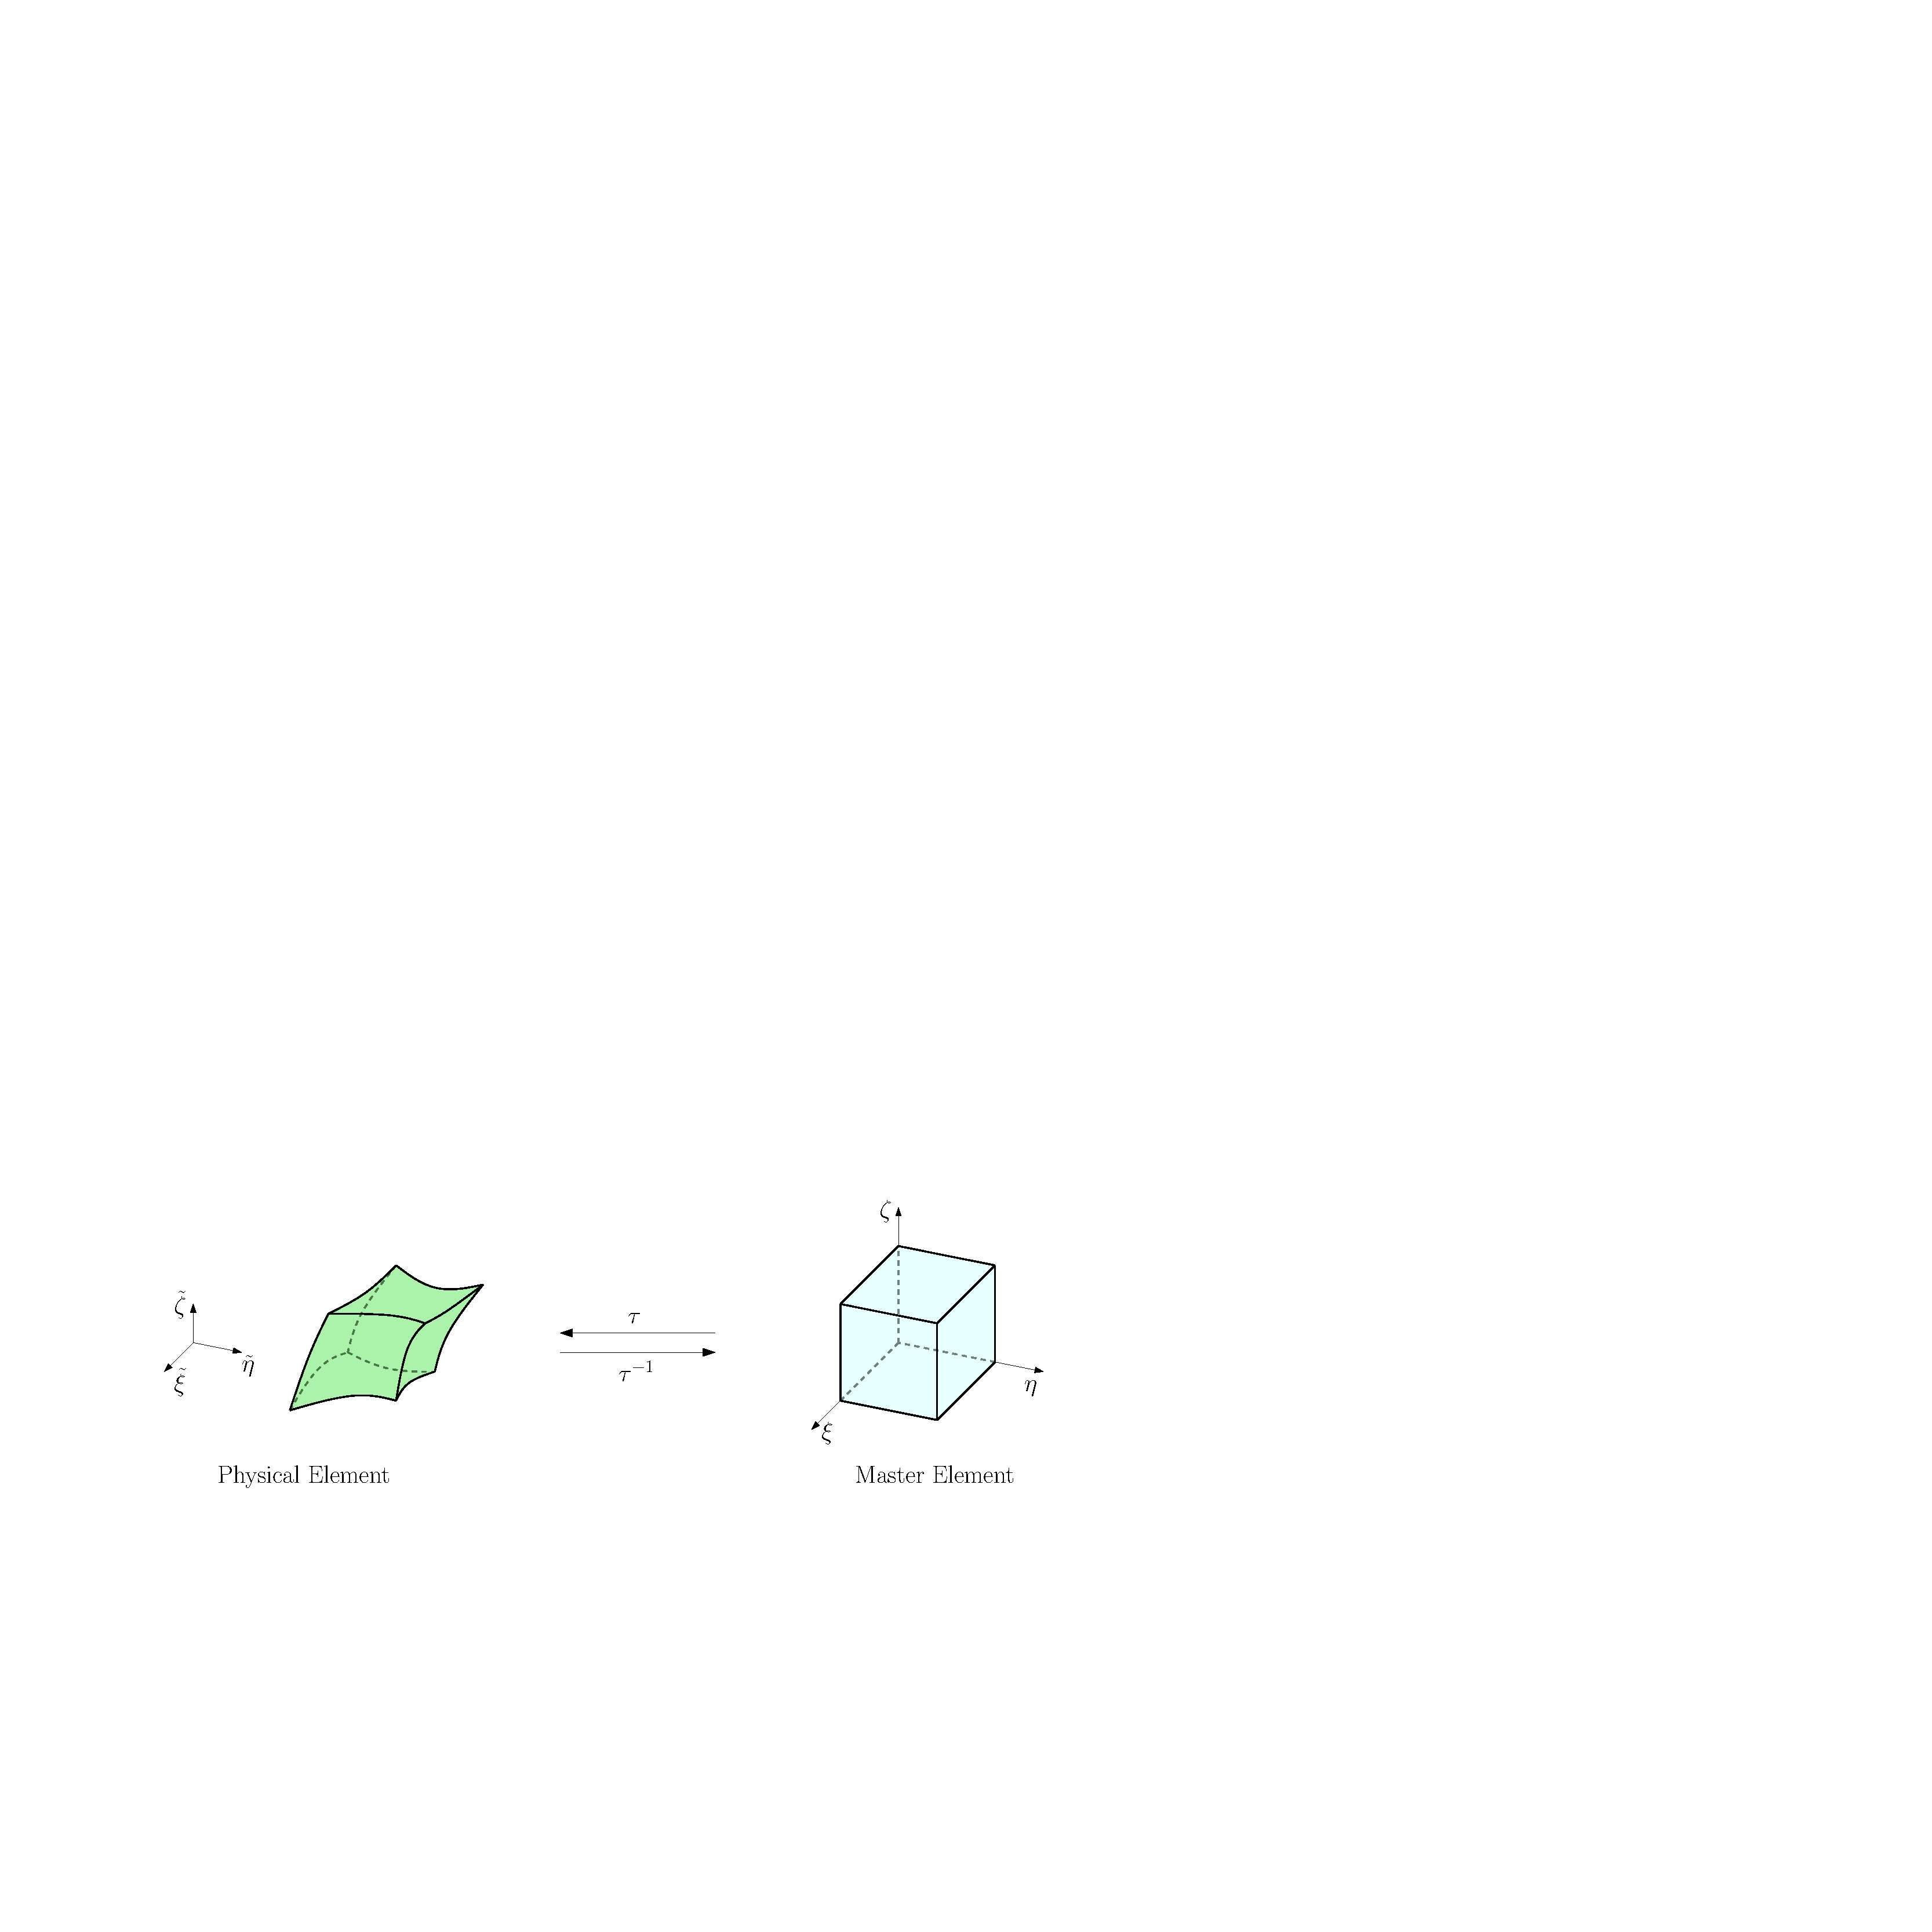
\includegraphics[scale=0.45]{./figures/CurvilinearTransform.pdf}
\caption{Transformation from the master element to the physical element.}\label{fig:curvilineartransform}
\end{center}
\end{figure}

At its core, the finite element method advocates carrying out integration over a master element domain instead of the original physical element.
It makes the method very feasible from a computational standpoint.
This involves a change of variables $\tau:\Omega\rightarrow\tilde{\Omega}$, from the master element domain $\Omega$ to the physical domain $\tilde{\Omega}$, which is assumed to be known.
This is illustrated in Figure \ref{fig:curvilineartransform}.
Note the change of variables $\tau$ is in general a nonlinear mapping.

Indeed, consider a ``physical'' integrand $f$ which is a function of variables in the different energy spaces and their differential form.
These variables are in the physical system of coordinates.
For instance, take $\phi_{\tilde{\Omega}}$, $E_{\tilde{\Omega}}$, $V_{\tilde{\Omega}}$ and $\psi_{\tilde{\Omega}}$ to represent variables in $H^1$, $H(\mathrm{curl})$, $H(\mathrm{div})$ and $L^2$ respectively.
Their corresponding differentials are $\nabla_{\tilde{\Omega}}\phi_{\tilde{\Omega}}$, $\nabla_{\tilde{\Omega}}\!\times\!E_{\tilde{\Omega}}$ and $\nabla_{\tilde{\Omega}}\!\cdot\!V_{\tilde{\Omega}}$.
However, it is their pullbacks to the master element domain, denoted with the subscript $\Omega$, which are known, since the shape functions are defined in the master element domain.\footnote{Unless the affine coordinates and their gradient are written in the physical system of coordinates, in which case one can simply substitute them in the expressions for the shape functions. This is due to the coordinate free nature of the shape functions.}
Making use of the appropriate pullback mapping for each of the variables as written in \eqref{eq:pullbacksgeneral}, this yields\footnote{In 2D, $\nabla_{\Omega}\!\times\!E_{\Omega}$ is in $L^2$, so the correct expression in the last line would be $\frac{1}{\det(J_\tau)}\nabla_{\Omega}\!\times\!E_{\Omega}$ instead of the 3D expression $\frac{1}{\det(J_\tau)}J_\tau\nabla_{\Omega}\!\times\!E_{\Omega}$. In 1D, $E_{\Omega}$ and $V_{\Omega}$ do not even exist, so they would be ignored throughout.}
\begin{equation}
	\begin{aligned}
		\mathcal{I}_{\tilde{\Omega}}&\!=\!\int_{\tilde{\Omega}}\!
			f\Big(\phi_{\tilde{\Omega}},\nabla_{\tilde{\Omega}}\phi_{\tilde{\Omega}},
				E_{\tilde{\Omega}},\nabla_{\tilde{\Omega}}\!\times\!E_{\tilde{\Omega}}, 
					V_{\tilde{\Omega}},\nabla_{\tilde{\Omega}}\!\cdot\!V_{\tilde{\Omega}}, \psi_{\tilde{\Omega}}\Big)\mathrm{d}\tilde{\Omega}\\
			&\!=\!\int_{\Omega}\!f\Big(\phi_{\tilde{\Omega}}\circ\tau, (\nabla_{\tilde{\Omega}}\phi_{\tilde{\Omega}})\circ\tau,
				E_{\tilde{\Omega}}\circ\tau,(\nabla_{\tilde{\Omega}}\!\times\!E_{\tilde{\Omega}})\circ\tau, 
					V_{\tilde{\Omega}}\circ\tau,(\nabla_{\tilde{\Omega}}\!\cdot\!V_{\tilde{\Omega}})\circ\tau,
						\psi_{\tilde{\Omega}}\circ\tau\Big)\!\det(J_\tau)\mathrm{d}\Omega\\
			&\!=\!\int_{\Omega}\!f\Big(\phi_{\Omega},J_\tau^{-\T}\nabla_{\Omega}\phi_{\Omega},
				J_\tau^{-\T}E_{\Omega},\textstyle{\frac{1}{\det(J_\tau)}}J_\tau\nabla_{\Omega}\!\times\!E_{\Omega},\\
					&\qquad\qquad\qquad\qquad\qquad\qquad\qquad\qquad\quad
						\textstyle{\frac{1}{\det(J_\tau)}}J_\tau V_{\Omega},\textstyle{\frac{1}{\det(J_\tau)}}\nabla_{\Omega}\!\cdot\!V_{\Omega},
							\textstyle{\frac{1}{\det(J_\tau)}}\psi_{\Omega}\Big)\!\det(J_\tau)\mathrm{d}\Omega\,,
	\end{aligned}
	\label{eq:integraluptomaster}
\end{equation}
where $J_\tau$ is the Jacobian matrix of the transformation $\tau:\Omega\rightarrow\tilde{\Omega}$.

Now, the integration is at least in a well known master element domain.
However, this is still a ``difficult'' domain over which to integrate (with the exception of the 1D segment, the 2D quadrilateral and the 3D hexahedron).
Hence, it is desirable to make one further change of coordinates to a ``nicer'' integration domain.
This is denoted by $\tau_Q:Q\rightarrow\Omega$, where $Q=(0,1)$ in 1D, $Q=(0,1)^2$ in 2D and $Q=(0,1)^3$ in 3D.
The transformations for each element are nicely depicted in Figure \ref{fig:integrationtransforms}. 
Some readers may have a strong preference for the integration domains $\tilde{Q}=(-1,1)$ in 1D, $\tilde{Q}=(-1,1)^2$ in 2D and $\tilde{Q}=(-1,1)^3$ in 3D.
If that is the case, then simply make the substitutions $x=\frac{\tilde{x}+1}{2}$, $y=\frac{\tilde{y}+1}{2}$ and $z=\frac{\tilde{z}+1}{2}$ in those expressions shown in Figure \ref{fig:integrationtransforms}.

%Variational methods require of integrating a function over a physical spatial domain.
%In particular the finite element method separates the domain into elements which are tranformed to the same basic set of master elements

\begin{figure}[!ht]
\begin{center}
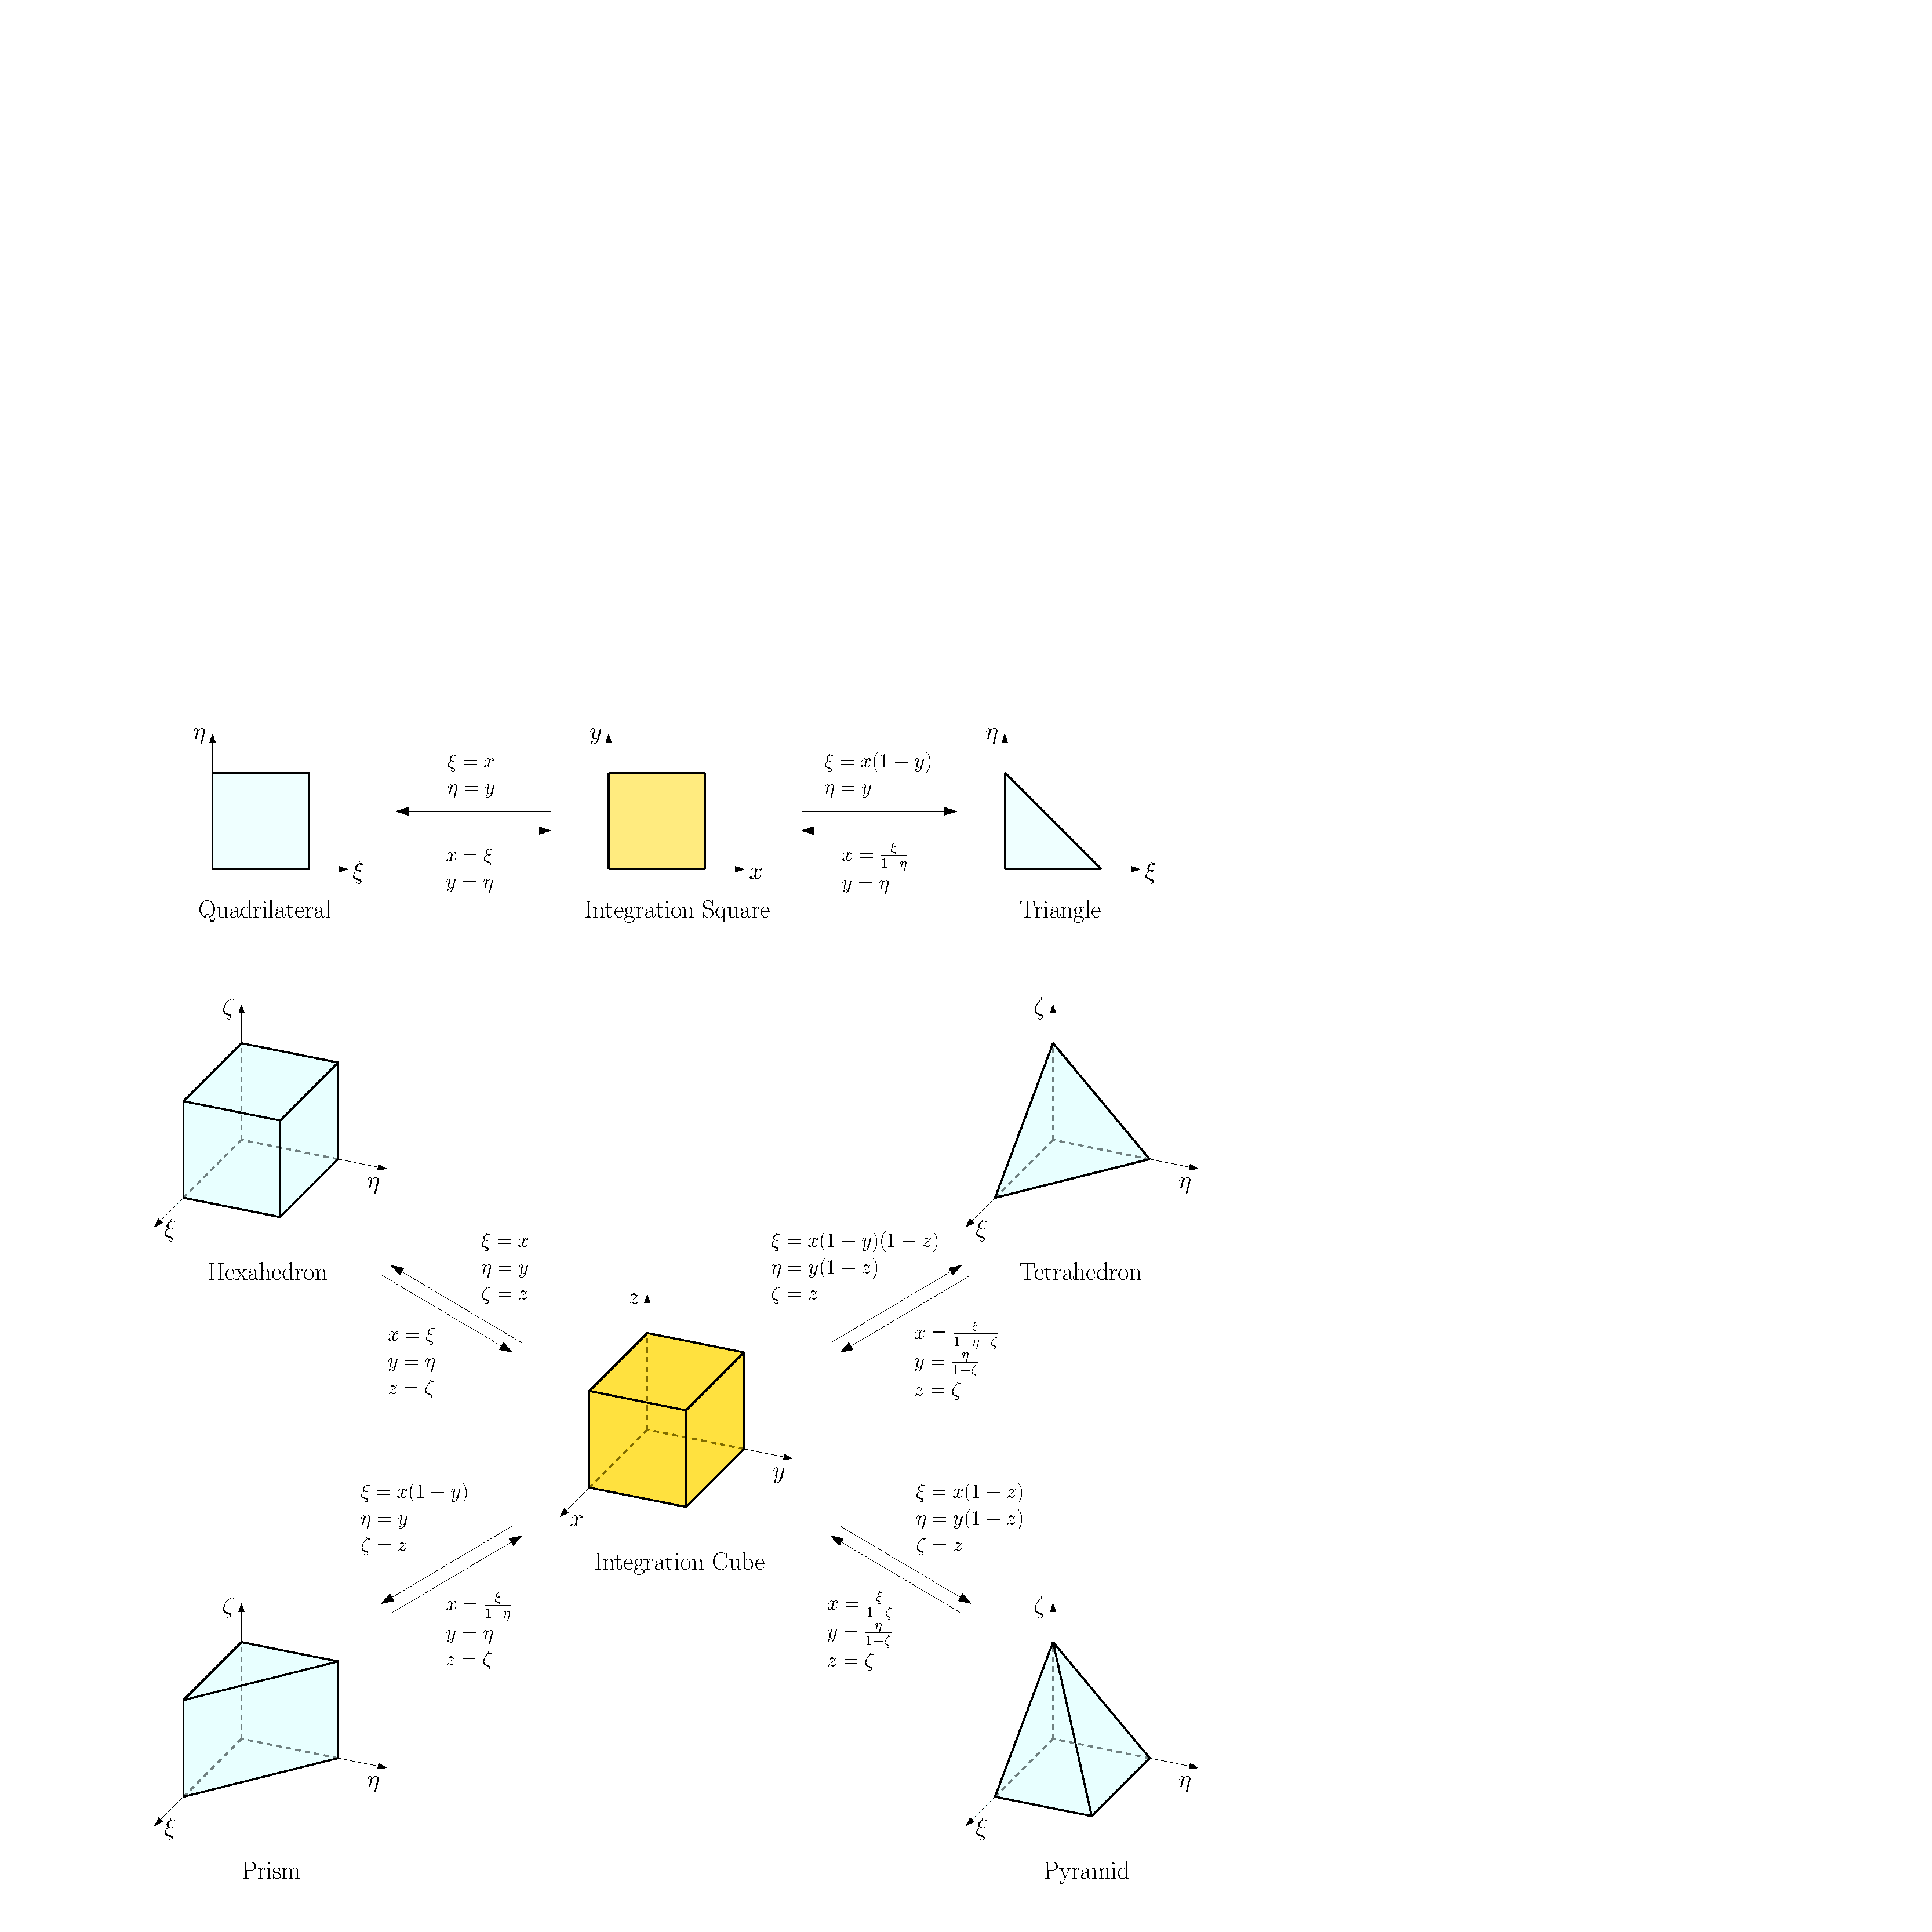
\includegraphics[scale=0.45]{./figures/IntegrationTransformations.pdf}
\caption{Transformations from each element to a nice integration domain.}\label{fig:integrationtransforms}
\end{center}
\end{figure}

%The finite element method requires integrating a function over the domain. 
%Computing these integrals over each element is therefore a fundamental step.
%Unfortunately, some elements do not have nice shapes, so it is convenient to transform them to a domain where integration is simpler to perform.
%The simplest of such domains is a square in 2D and a cube in 3D.
%Indeed, it is possible to tranform from each element to an integration square or cube as evidenced in Figure \ref{fig:integrationtransforms}.
%Note the transformations (except for the hexahedron) are nonlinear. 

The original integral in \eqref{eq:integraluptomaster} finally becomes
\begin{equation}
	\begin{aligned}
		\mathcal{I}_{\tilde{\Omega}}
			&\!=\!\int_{Q}\!f\Big(\phi_{\Omega}\circ\tau_Q,(J_\tau^{-\T}\nabla_{\Omega}\phi_{\Omega})\circ\tau_Q,
				(J_\tau^{-\T}E_{\Omega})\circ\tau_Q,(\textstyle{\frac{1}{\det(J_\tau)}}J_\tau\nabla_{\Omega}\!\times\!E_{\Omega})\circ\tau_Q,\\
					&\qquad\qquad
						(\textstyle{\frac{1}{\det(J_\tau)}}J_\tau V_{\Omega})\circ\tau_Q,
							(\textstyle{\frac{1}{\det(J_\tau)}}\nabla_{\Omega}\!\cdot\!V_{\Omega})\circ\tau_Q,
								(\textstyle{\frac{1}{\det(J_\tau)}}\psi_{\Omega})\circ\tau_Q\Big)\!\det(J_{\tau_Q})\det(J_\tau)\mathrm{d}Q\,,
	\end{aligned}
	\label{eq:integraluptoQ}
\end{equation}
where $J_{\tau_Q}$ is the Jacobian matrix of the transformation $\tau_Q:Q\rightarrow\Omega$.

\subsection{Fast integration}

To actually calculate the integral, the typical approach is to use Gaussian quadrature.
In $Q$ (or $\tilde{Q}$) the quadrature points and weights are well known and taken from the literature, and this is part of the reason why integration over the physical domain was reduced to integration over $Q$ in \eqref{eq:integraluptoQ}.

However, as the number of spatial dimensions $N$ increases from 1D to 3D, the cost grows quickly with $p$.
Indeed, to construct a typical finite element stiffness matrix, integrals usually reduce to the form
\begin{equation*}
	\mathcal{I}_{\tilde{\Omega}}=\int_{Q}u_Iv_J\mathrm{d}Q\,,
\end{equation*}
where $I=1,\ldots,\mathcal{O}(p^N)$ and $J=1,\ldots,\mathcal{O}(p^N)$.
The cost to integrate each term is $\mathcal{O}(p^N)$ as well, because there are $p+1$ quadrature points in each spatial dimension.
Hence, with a straightforward implementation, the cost to integrate all terms is $\mathcal{O}(p^{3N})$, so it is $\mathcal{O}(p^3)$ in 1D, $\mathcal{O}(p^6)$ in 2D and $\mathcal{O}(p^9)$ in 3D.
This constitutes a problem for $N\geq2$ and high $p$, so it is highly desirable to improve the integration cost.

Fortunately, the integration cost can be reduced if there exists a decoupling of either $u_I$ or $v_J$ in $x$, $y$ and $z$ (the variables after transforming to $Q$, not necessarily the variables of the physical or master element domain). 
Assume the decoupling is in $v_J$, where it takes the form $v_J(x,y)=v_{j_x}^x(x,y)v_{j_y}^y(y)$ in 2D and $v_J(x,y,z)=v_{j_x}^x(x,y,z)v_{j_y}^y(y,z)v_{j_z}^z(z)$ in 3D, with $j_x,j_y,j_z=1,\ldots,\mathcal{O}(p)$. 
Then, by reorganizing the operations and storing some coefficients, the cost is reduced to $\mathcal{O}(p^5)$ in 2D, and to $\mathcal{O}(p^7)$ in 3D.
Some of the details are in \citet{hpbook2}.
With the shape functions presented in this text, regardless of the element shape and the the associated topological entity, such a decoupling is to be expected, so this acceleration to $\mathcal{O}(p^{2N+1})$ is possible.
This technique based on a tensor product decoupling is typically called \textit{fast quadrature}.

Naturally, there are other fast integration techniques different from the fast quadrature described above which might also be applicable, but further research is required.

%Appendix D
\newpage
\pagenumbering{arabic}% resets counter to 1
\renewcommand*{\thepage}{\thesection-\arabic{page}}%Custom numbering
\section{Verification}
\label{app:verification}

%\subsection{Polynomial Reproducibility}

One of the most important tests is to numerically confirm the polynomial approximability properties of the spaces spanned by the shape functions.
Coupled with the exact sequence property of the discrete spaces, this ensures all well known interpolation inequalities.
More specifically, for an affinely transformed master element mesh, let $W^p$ be the span of the $H^1$ basis functions of order $p$ (being composed piecewise by shape functions), and similarly with $Q^p$, $V^p$ and $Y^p$ for the spaces $H(\mathrm{curl})$, $H(\mathrm{div})$ and $L^2$ respectively.
Then, one has to check that $\mathcal{P}^p\subseteq W^p$, $(\mathcal{P}^{p-1})^3\subseteq Q^p$, $(\mathcal{P}^{p-1})^3\subseteq V^p$ and $\mathcal{P}^{p-1}\subseteq Y^p$.

To do this, first consider an arbitrary $u$ in a given energy space $U$ approximated by a discrete space $U_h$.
Clearly,
\begin{equation}
	u\in U_h \Leftrightarrow \mathrm{dist}(u,U_h)=\min_{u_h\in U_h}||u-u_h||_U=0\,.
\end{equation}
Hence, given $u\in U$ the task is to compute $\mathrm{dist}(u,U_h)=||u-u_h||_U$, with $u_h\in U_h$ being the element where the minimum is attained.
Fortunately $u_h$ is computed from a variational problem equivalent to the projection (distance) problem.
It is,
\begin{equation}
	||u-u_h||_U=\mathrm{dist}(u,U_h)\Leftrightarrow
		\begin{cases}
			u_h\in U_h\,,&{}\\
			b(u_h,v_h)=\langle u_h,v_h \rangle_U=\langle u,v_h \rangle_U=\ell_u(v_h)& \forall v_h\in U_h.
		\end{cases}
	\label{eq:variationalprojection}
\end{equation}
Naturally, the inner product is different depending on the energy space $U$.
They are,
\begin{equation}
  \begin{aligned}
	  \langle \phi_1,\phi_2\rangle_{H^1}&=\int_\Omega (\phi_1\phi_2+\nabla\phi_1\cdot\nabla\phi_2)\mathrm{d}\Omega\,,\\
	  \langle E_1,E_2\rangle_{H(\mathrm{curl})}&=\int_\Omega (E_1\cdot E_2+(\nabla\times E_1)\cdot(\nabla\times E_2))\mathrm{d}\Omega\,,\\
		\langle V_1,V_2\rangle_{H(\mathrm{div})}&=\int_\Omega (V_1\cdot V_2+(\nabla\cdot V_1)(\nabla\cdot V_2))\mathrm{d}\Omega\,,\\
		\langle \psi_1,\psi_2\rangle_{L^2}&=\int_\Omega \psi_1\psi_2\mathrm{d}\Omega\,.
	\end{aligned}
\end{equation}

Then, the task is to determine whether each element $u$ of a monomial basis for the polynomial spaces in question lies in $U_h$.
This is achieved by solving the variational problem in \eqref{eq:variationalprojection} and checking that the relative error $\frac{||u-u_h||_U}{||u||_U}=\frac{\mathrm{dist}(u,U_h)}{||u||_U}$ is in the range of machine zero.
Thus, for example to ensure that $\mathcal{P}^p\subseteq W^p$ one must check that all monomials of the form $x^iy^jz^k$ for $i+j+k\leq p$ lie in $W^p$, the span of the $H^1$ basis functions.
Similar procedures hold for $H(\mathrm{curl})$, $H(\mathrm{div})$ and $L^2$.
These tests are called \textit{polynomial reproducibility} tests.

The polynomial reproducibility tests are successful when using the code associated with this work.
The tests are done on a series of meshes, including a four element hybrid mesh with one element of each type, as depicted in Figure \ref{fig:VerificationMesh}.
By doing this on a mesh, there is the additional value of implicitly verifying compatibility of the shape functions across the boundaries of the elements.
Indeed, it should be checked that the polynomial reproducibililty tests pass under all possible orientations of each face and edge in the mesh, which is the case for our code.

\begin{figure}[!ht]
\begin{center}
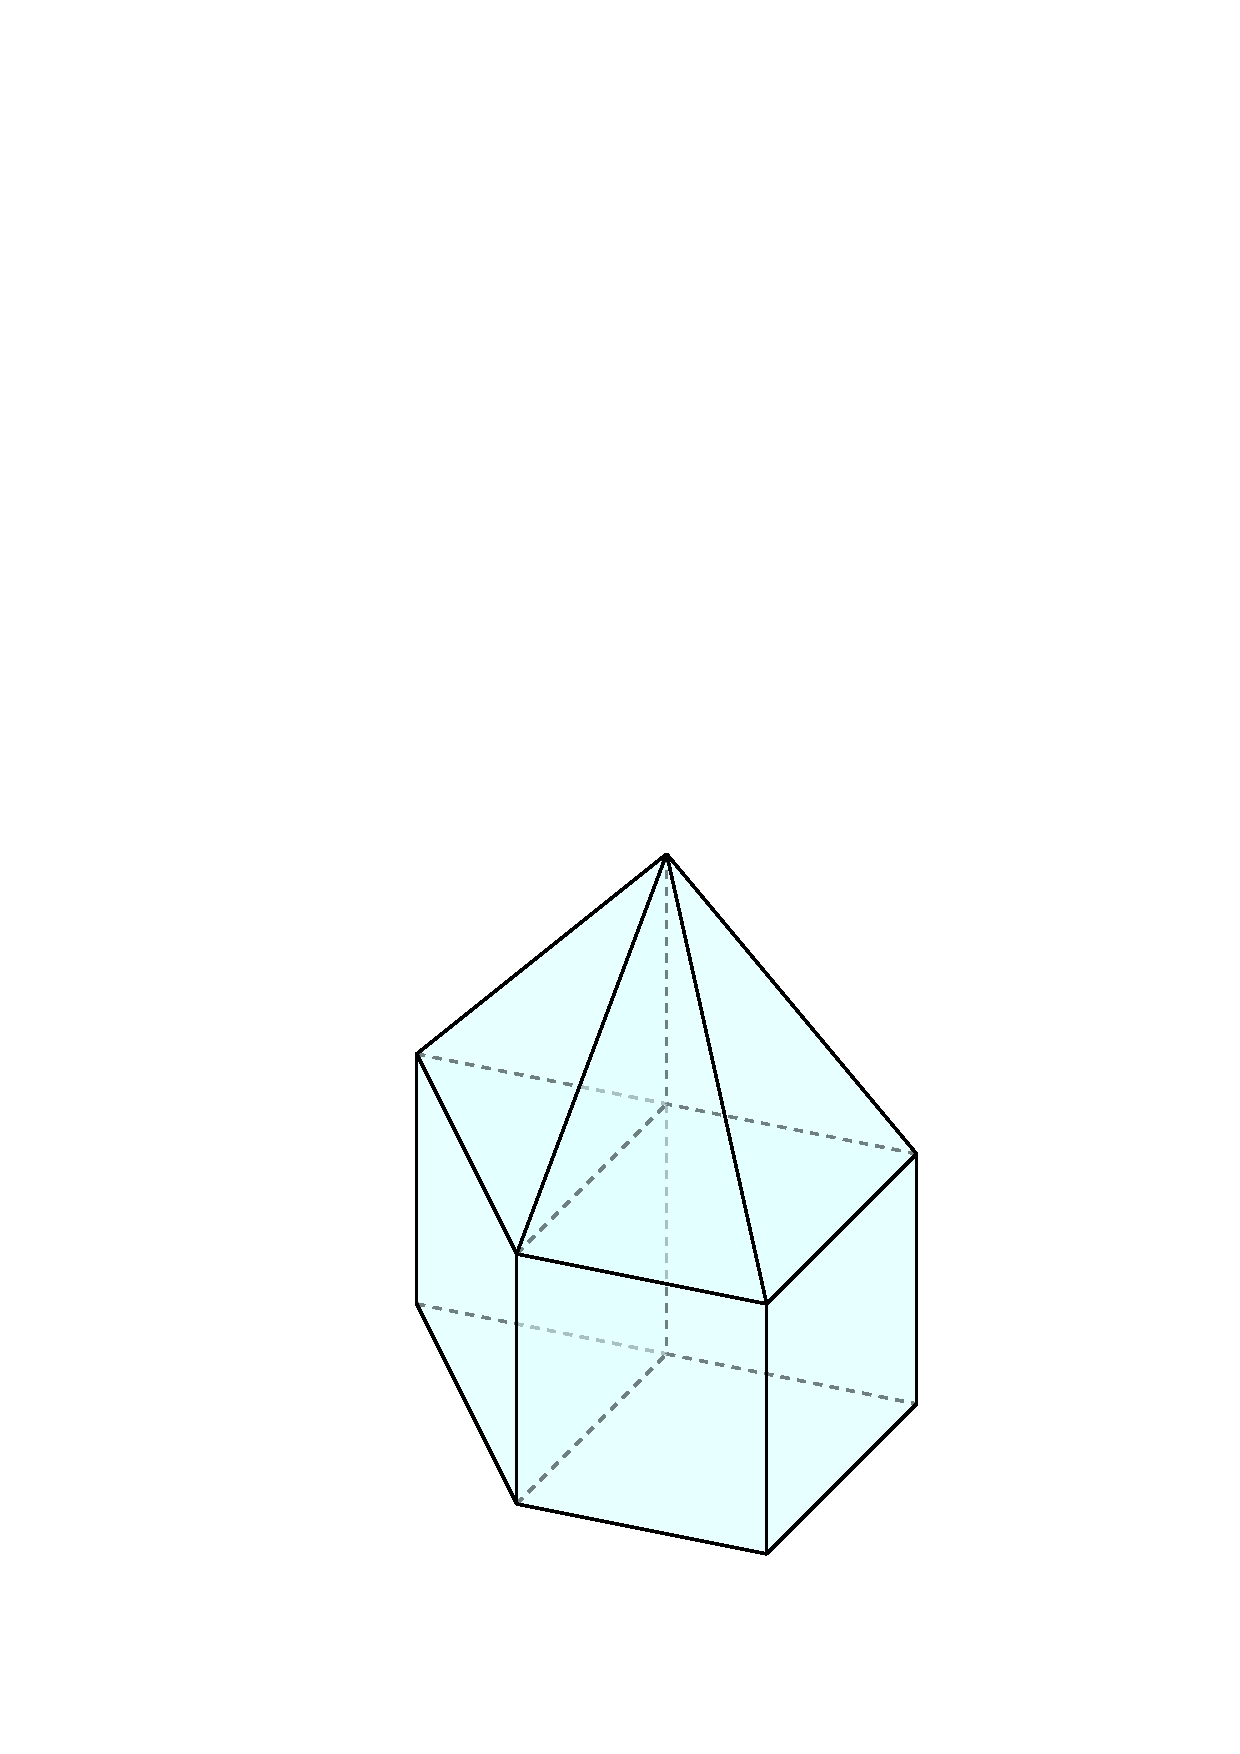
\includegraphics[scale=0.5]{./figures/VerificationMesh.pdf}
\caption{A hybrid mesh used to verify polynomial reproducibility.}
\label{fig:VerificationMesh}
\end{center}
\end{figure}

%\subsection{Exact Sequence Properties}

Another convenient test is to verify some aspects of the exact sequence property of the discrete spaces.
For this, consider a fixed element and the discrete spaces $W^p$, $Q^p$, $V^p$ and $Y^p$ conforming to $H^1$, $H(\mathrm{curl})$, $H(\mathrm{div})$ and $L^2$ respectively.
The discrete spaces are precisely the span of the corresponding shape functions.

Hence, for example consider an $H^1$ shape function $\phi\in W^p$.
Then the idea is to confirm numerically that $\nabla\phi\in Q^p$.
This is done as described in the polynomial reproducibility tests, where the computed projection of $\nabla\phi$ to $Q^p$ is $E_h$, which is given as a linear combination of the $H(\mathrm{curl})$ shape functions $E\in Q^p$.
Therefore, one should obtain that that $\frac{||\nabla\phi-E_h||_{H(\mathrm{curl})}}{||\nabla\phi||_{H(\mathrm{curl})}}$ is in the range of machine zero.
Moreover, one can additionally check that the coefficients of the linear combination for $E_h$ make sense.
For instance, if $\phi\in W^p$ is originally an $H^1$ interior bubble, then $\nabla\phi$ is also an $H(\mathrm{curl})$ interior bubble and as a result is in the span of the $H(\mathrm{curl})$ interior shape functions (meaning the coefficients associated to $H(\mathrm{curl})$ edge and face shape functions are zero).
Similarly, if $\phi\in W^p$ is an $H^1$ face shape function, then $\nabla\phi$ is in the span of the the $H(\mathrm{curl})$ face functions associated to the same face \textit{and} the $H(\mathrm{curl})$ interior bubbles.
Naturally this applies to other topological entities and to the different energy spaces.

These verifications are successful when using the code that supplements this text.


%\begin{equation}
%\begin{aligned}
%	u\in U_h&\Leftrightarrow \mathrm{dist}(u,U_h)=\min_{u_h\in U_h}||u-u_h||_U=0\\&\Leftrightarrow
%		\begin{cases}
%			u_h\in U_h\,,&{}\\
%			b(u_h,v_h)=\langle u_h,v_h \rangle_U=\langle u,v_h \rangle_U=\ell_u(v_h)& \forall v_h\in U_h.
%		\end{cases}
%\end{aligned}
%\end{equation}
%This is called the projection problem to $U_h$ from $U$

%
%\subsection{Reproducing Polynomials.}
%
%Consider the $H^1$-projection problem:
%$$
%\int_{\Omega} [(\bfnab u_h - \bfnab u) \bfnab v_h + (u_h - u) v_h] = 0
%\quad \forall v_h \, .
%$$
%If projected function $u$ lives in the FE space, the FE solution $u_h$ must coincide
%with $u$ up to machine precision, and the corresponding relative $H^1$ error is expected
%to be of order $10^{-15}$. Given the four element mesh shown in
%Fig.~\ref{fig:verification} with order\footnote{More precisely, the tet and pyramid
%are of order $p$, hexa is of order $ppp$, and prism is of order $pp$.} of elements set to $p$,
% we loop through monomials
%$$
%u = x^i y^j z^k,\quad i,j,k \geq 0,\,  i+j+k \leq p\, ,
%$$
%and verify that, for each projected monomial, the projection error is indeed in the range of machine zero.
%
%We perform the same test for $H(\text{curl})$-conforming elements and $H(\text{curl})$ projection,
%$$
%\int_{\Omega} [(\bfnab \times E_h - \bfnab \times E) \cdot \bfnab \times F_h + (E_h - E) \cdot F_h] = 0
%\quad \forall F_h \, ,
%$$
%using several familes of vector polynomials $E$,
%$$
%\begin{array}{ll}
%E = x^i y^j z^k e \quad & i,j,k \geq 0,\,  i+j+k \leq p-1\, ,\\
%E = x^i y^j z^k (x,y,z) \times \bfe & i,j,k \geq 0,\,  i+j+k = p-1\,
%\end{array}
%$$
%where $e = (1,0,0), \, (0,1,0), \, (0,0,1)$.
%
%
%Similarly, for $H(\text{div})$-conforming elements we use the $H(\text{div})$ projection,
%$$
%\int_{\Omega} [(\bfnab \cdot V_h - \bfnab \cdot V) \bfnab \cdot W_h + (V_h - V) \cdot W_h] = 0
%\quad \forall W_h \, ,
%$$
%using the following familes of vector polynomials $V$,
%$$
%\begin{array}{ll}
%F = x^i y^j z^k e \quad & i,j,k \geq 0,\,  i+j+k \leq p-1\, ,\\
%F = x^i y^j z^k (x,y,z)  & i,j,k \geq 0,\,  i+j+k = p-1\, .
%\end{array}
%$$
%Finally, we use the $L^2$-projection and monomials of order $p-1$ to verify the $L^2$-conforming
%elements.
%
%
%
%
%
%
%\begin{figure}[ht!]
%\begin{center}
%\includegraphics[angle=0,width=0.50\textwidth]{./figures/verification.png}
%\end{center}
%\caption{Four element mesh used for the verification.
%}
%\label{fig:verification}
%\end{figure}
%
%
%\subsection{Verifying Orientations.} In the next test, for every edge and every face
%in the mesh, we loop through all possible edge and face orientations (two for edge, six for a triangle,
%and eight for a square) and, for each modified orientation, perform the projection test
%described above. All edges and faces are explicitly defined in a geometry input file
%by listing the corresponding edge-to-vertex and face-to-vertex connectivities. Changing
%the orientations reduces thus to listing the vertices in a different order. For instance,
%the vertices for square face $1265$ undergo the following permutations:
%$$
%1265,\quad 2651,\quad 6512,\quad 5126,\quad 1562,\quad 2156,\quad 6215,\quad 5621 \, .
%$$
%
%\subsection{Verifying Exact Polynomial Complex Property}
%
%One of the tools that we have found very useful
%was the verification of the polynomial complex property. For instance, the $H(\text{curl})$ elements
%(one element at a time) we debugged by using $E = \bfnab u_h$ where $u_h$ is an $H^1$ shape function.
%Not only we know that the correponding projection error must be zero but also we know ahead of time
%which $H(\text{curl})$ shape functions should contribute to (``connect with'') the projection.
%For instance, if $u_h$ is an element $H^1$ bubble then $E_h$ must also be an element  $H(\text{curl})$
%bubble. Similarly, if $u_h$ is a face bubble then $E_h$ must live in the span of the same face
%$H(\text{curl})$ bubbles and element bubbles, etc. This verification helped to eliminate not only
%coding errors but also a few theoretical omittments (for the pyramid) as well.
%
%\subsection{Other Useful Debugging Tools}
%
%When encountering an error in performing the projection tests for the $H(\text{curl})$
%and $H(\text{div})$, we frequently switched to $L^2$ projections. This helps to separate debugging
%the formulas for the $H(\text{curl})$
%and $H(\text{div})$ shape functions from the corresponding formulas for their curl and divergence.

%Appendix E
\newpage
\pagenumbering{arabic}% resets counter to 1
\renewcommand*{\thepage}{\thesection-\arabic{page}}%Custom numbering
\section{Tables}
\label{app:ShapeFunctionTable}

\subsection{Polynomials}

%%%%%%%%%%%%%%%%%%%%%Polynomials 1: Legendre%%%%%%%%%%%%%%%%%%%%%
\renewcommand{\arraystretch}{1.35}%Better row spacing
\begin{center}
\begin{tabular}
{|C{0.35cm} L{11.9cm} C{2.9cm}|N}%See main file for this custom columns - they keep a fixed width while maintaining aligment
\hline
\multicolumn{3}{|c|}{\large \textbf{Polynomials}} &\\
\hline
\multicolumn{3}{|c|}{Legendre} &\\
\hline
{}& {} &{} &\\[-23pt]%To keep total width fixed
\multicolumn{3}{|l|}{Shifted and scaled Legendre polynomials for $t\geq0$ and $x\in[0,t]$:} &\\
\multicolumn{3}{|l|}{
$\begin{aligned}
	P_0(x;t)&=1\\
	P_1(x;t)&=2x-t\\
	iP_i(x;t)&=(2i-1)(2x-t)P_{i-1}(x;t)-(i-1)t^2P_{i-2}(x;t) \quad \text{for }\, i\geq2
\end{aligned}$} &\\
\multicolumn{3}{|l|}{Integrated Legendre polynomials:} &\\
\multicolumn{3}{|l|}{
$	\begin{aligned}
		2(2i-1)L_i(x; t)&=P_i(x;t)-t^2P_{i-2}(x;t) \quad\text{for }\, i\geq2
	\end{aligned}$} &\\
\multicolumn{3}{|l|}{Scaling differential of integrated Legendre polynomials:} &\\
\multicolumn{3}{|l|}{
$	\begin{aligned}
		\textstyle{\frac{\partial}{\partial t}}L_{i+1}(x;t)
			&=R_i(x;t)=-\textstyle{\frac{1}{2}}(P_i(x;t)+tP_{i-1}(x;t))\quad\text{for }\,i\geq1
	\end{aligned}$} &\\
\multicolumn{3}{|l|}{Homogenized polynomials:} &\\
\multicolumn{3}{|l|}{
$	\begin{aligned}{}
		[P_i](s_0,s_1)&=P_i(s_1;s_0+s_1)\quad\text{for }\, i\geq0\\
		[R_i](s_0,s_1)&=R_i(s_1;s_0+s_1)\quad\text{for }\, i\geq1\\
		[L_i](s_0,s_1)&=L_i(s_1;s_0+s_1)\quad\text{for }\, i\geq2\\
		\nabla[L_i](s_0,s_1)&=[P_{i-1}](s_0,s_1)\nabla s_1+[R_{i-1}](s_0,s_1)\nabla(s_0+s_1)
			\quad\text{for }\, i\geq2
	\end{aligned}$} &\\	
\multicolumn{3}{|l|}{$\,\,$ where $s_0$ and $s_1$ are functions of some spatial variable in $\R^N$, so $\nabla s_0,\nabla s_1\in\R^N$, for $N=1,2,3$.} &\\[-17pt]
{}& {} &{} &\\[-5pt]
\multicolumn{3}{r}{\footnotesize\textit{continued on next page}} &\\[-18.5pt]
\hline
\end{tabular}
\end{center}
\renewcommand{\arraystretch}{1}%Back to normal spacing

\newpage

%%%%%%%%%%%%%%%%%%%%%Polynomials 2: Jacobi%%%%%%%%%%%%%%%%%%%%%
\renewcommand{\arraystretch}{1.35}%Better row spacing
\begin{center}
\begin{tabular}
{|C{0.35cm} L{11.9cm} C{2.9cm}|N}%See main file for this custom columns - they keep a fixed width while maintaining aligment
\multicolumn{3}{l}{\footnotesize\textit{continued from previous page}} &\\[-2pt]
\hline
\multicolumn{3}{|c|}{\large \textbf{Polynomials}} &\\
\hline
\multicolumn{3}{|c|}{Jacobi} &\\
\hline
{}& {} &{} &\\[-23pt]%To keep total width fixed
\multicolumn{3}{|l|}{Shifted and scaled Jacobi polynomials for $\alpha>-1$, $t\geq0$ and $x\in[0,t]$:} &\\
\multicolumn{3}{|l|}{
$	\begin{aligned}
		P_0^\alpha(x;t) &= 1 \\
		P_1^\alpha(x;t) &= 2x-t+\alpha x\\
		a_j{P}_j^\alpha(x;t)&=b_j(c_j(2x-t)+\alpha^2 t)P_{j-1}^\alpha(x;t)-d_jt^2 P_{j-2}^\alpha(x;t)
		\quad \text{for }\, j\geq2
	\end{aligned}$} &\\
\multicolumn{3}{|l|}{$\,\,$ where} &\\
\multicolumn{3}{|l|}{
$	\begin{aligned}{}
		\qquad a_j &=  2j(j+\alpha)\, (2j + \alpha - 2)\\
		\qquad b_j &=  2j + \alpha - 1\\
		\qquad c_j &=  (2j+\alpha)\, (2j + \alpha - 2)\\
		\qquad d_j &=  2(j+\alpha-1)\, (j-1)\, (2j+\alpha)
	\end{aligned}$} &\\
\multicolumn{3}{|l|}{Integrated Jacobi polynomials:} &\\
\multicolumn{3}{|l|}{
$	\begin{aligned}
		L^{\alpha}_1(x;t)&= x\\
		L^{\alpha}_j(x;t)&=a_j P^{\alpha}_j(x,t)+b_jtP^{\alpha}_{j-1}(x;t)-c_jt^2P^{\alpha}_{j-2}(x;t)
			\quad\text{for }\, j\geq2
	\end{aligned}$} &\\
\multicolumn{3}{|l|}{$\,\,$ where} &\\
\multicolumn{3}{|l|}{
$	\begin{aligned}{}
		\qquad a_j = & \textstyle{\frac{j + \alpha}{(2j + \alpha -1)(2j + \alpha)}} \\
		\qquad b_j = & \textstyle{\frac{\alpha}{(2j + \alpha -2)(2j + \alpha)}} \\
		\qquad c_j = & \textstyle{\frac{j-1}{(2j + \alpha -2)(2j + \alpha-1)}}
	\end{aligned}$} &\\
\multicolumn{3}{|l|}{Scaling differential of integrated Jacobi polynomials:} &\\
\multicolumn{3}{|l|}{
$	\begin{aligned}
		\textstyle{\frac{\partial}{\partial t}}L_1^\alpha(x;t)&=R_0^\alpha(x;t)=0\\
		\textstyle{\frac{\partial}{\partial t}}L_{j+1}(x;t)
			&=R^\alpha_j(x;t) = -\textstyle{\frac{j}{2j+\alpha}}(P^\alpha_j(x;t)+tP^\alpha_{j-1}(x;t))
				\quad\text{for }\,j\geq1
	\end{aligned}$} &\\
\multicolumn{3}{|l|}{Homogenized polynomials:} &\\
\multicolumn{3}{|l|}{
$	\begin{aligned}{}
		[P_j^\alpha](t_0,t_1)&=P_j^\alpha(t_1;t_0+t_1)\quad\text{for }\, j\geq0\\
		[R_j^\alpha](t_0,t_1)&=R_j^\alpha(t_1;t_0+t_1)\quad\text{for }\, j\geq0\\
		[L_j^\alpha](t_0,t_1)&=L_j^\alpha(t_1;t_0+t_1)\quad\text{for }\, j\geq1\\
		\nabla[L_j^\alpha](t_0,t_1)&=[P_{j-1}^\alpha](t_0,t_1)\nabla t_1+[R_{j-1}^\alpha](t_0,t_1)\nabla(t_0+t_1)
			\quad\text{for }\, j\geq1
	\end{aligned}$} &\\	
\multicolumn{3}{|l|}{$\,\,$ where $t_0$ and $t_1$ are functions of some spatial variable in $\R^N$, so $\nabla t_0,\nabla t_1\in\R^N$, for $N=1,2,3$.} &\\[-17pt]
{}& {} &{} &\\
\hline
\end{tabular}
\end{center}
\renewcommand{\arraystretch}{1}%Back to normal spacing

\newpage
\subsection{Ancillary Operators}

%%%%%%%%%%%%%%%%%%%%%Ancillary 1: H1 and Hcurl%%%%%%%%%%%%%%%%%%%%%
\renewcommand{\arraystretch}{1.35}%Better row spacing
\begin{center}
\begin{tabular}
{|C{0.35cm} L{11.9cm}|C{2.9cm}|N}%See main file for this custom columns - they keep a fixed width while maintaining aligment
\hline
\multicolumn{3}{|c|}{\large \textbf{Ancillary Operators}} &\\
\hline
\multicolumn{3}{|c|}{\small In all cases, $s_0$, $s_1$, $s_2$, $t_0$ and $t_1$ are functions of some spatial variable in $\R^N$.} &\\
\hline
\multicolumn{3}{|c|}{$H^1$} &\\
\hline
{}& {} &{} &\\[-23pt]%To keep total width fixed
\multicolumn{2}{|c|}{Operator}& Indices &\\ \hline
\multicolumn{2}{|l|}{Edge} &
\multirow{2}{*}[-12pt]{\small$\begin{gathered}
N\!=\!1,2,3\\
i\!=\!2,\ldots,p_s
\end{gathered}$} &\\
\multicolumn{2}{|l|}{
$	\begin{aligned}
		\phi^\E_i(s_0,s_1)&=[L_i](s_0,s_1)\\
		\nabla\phi^\E_i(s_0,s_1)&=\nabla[L_i](s_0,s_1)
	\end{aligned}$} &{}&\\
\multicolumn{2}{|l|}{Quadrilateral Face} &
\multirow{2}{*}[-5pt]{\small$\begin{gathered}
N\!=\!2,3\\
i\!=\!2,\ldots,p_s\\
j\!=\!2,\ldots,p_t
\end{gathered}$} &\\
\multicolumn{2}{|l|}{
$	\begin{aligned}
		\phi_{ij}^\square(s_0,s_1,t_0,t_1)&=\phi_i^\E(s_0,s_1)\phi_j^\E(t_0,t_1)\\
		\nabla\phi_{ij}^\square(s_0,s_1,t_0,t_1)&=\phi_i^\E(s_0,s_1)\nabla\phi_j^\E(t_0,t_1)+\phi_j^\E(t_0,t_1)\nabla\phi_i^\E(s_0,s_1)
	\end{aligned}$} &{}&\\
\multicolumn{2}{|l|}{Triangle Face} &
\multirow{2}{*}[-5pt]{\small$\begin{gathered}
N\!=\!2,3\\
i\geq2,\,j\geq1\\
i\!+\!j\!=\!3,\ldots,p_s
\end{gathered}$} &\\
\multicolumn{2}{|l|}{
$	\begin{aligned}
		\phi_{ij}^\Tri(s_0,s_1,s_2)&=\phi_i^\E(s_0,s_1)[L_j^{2i}](s_0+s_1,s_2)\\
		\nabla\phi_{ij}^\Tri(s_0,s_1,s_2)&=[L_j^{2i}](s_0\!+\!s_1,s_2)\nabla\phi_i^\E(s_0,s_1)
			+\phi_i^\E(s_0,s_1)\nabla[L_j^{2i}](s_0\!+\!s_1,s_2)
	\end{aligned}$} &{}&\\[-17pt]
{}& {} &{} &\\
\hline
\multicolumn{3}{|c|}{$H(\mathrm{curl})^\star$} &\\
\hline
{}& {} &{} &\\[-23pt]%To keep total width fixed
\multicolumn{2}{|c|}{Operator}& Indices &\\ \hline
\multicolumn{2}{|l|}{Edge$^\diamond$} &
\multirow{2}{*}[-12pt]{\small$\begin{gathered}
N\!=\!2,3\\
i\!=\!0,\ldots,p_s\!-\!1
\end{gathered}$} &\\
\multicolumn{2}{|l|}{
$	\begin{aligned}
		E^\E_i(s_0,s_1)&=[P_i](s_0,s_1)(s_0\nabla s_1-s_1\nabla s_0)\\
		\nabla\!\times\! E_i^\E(s_0,s_1)&=(i+2)[P_i](s_0,s_1)\nabla s_0\!\times\!\nabla s_1
	\end{aligned}$} &{}&\\
\multicolumn{2}{|l|}{Quadrilateral Face} &
\multirow{2}{*}[-5pt]{\small$\begin{gathered}
N\!=\!2,3\\
i\!=\!0,\ldots,p_s\!-\!1\\
j\!=\!2,\ldots,p_t
\end{gathered}$} &\\
\multicolumn{2}{|l|}{
$	\begin{aligned}
		E_{ij}^{\square}(s_0,s_1,t_0,t_1)&=\phi_j^\E(t_0,t_1)E_i^\E(s_0,s_1)\\
		\nabla\!\times\! E_{ij}^{\square}(s_0,s_1,t_0,t_1)&=\phi_j^\E(t_0,t_1)\nabla\!\times\! E_i^\E(s_0,s_1)
    	+\nabla\phi_j^\E(t_0,t_1)\!\times\! E_i^\E(s_0,s_1)
	\end{aligned}$} &{}&\\
\multicolumn{2}{|l|}{Triangle Face} &
\multirow{2}{*}[-12pt]{\small$\begin{gathered}
N\!=\!2,3\\
i\geq0,\,j\geq1\\
i\!+\!j\!=\!1,\ldots,p_s\!-\!1
\end{gathered}$} &\\
\multicolumn{2}{|l|}{
$	\begin{aligned}
		E_{ij}^\Tri(s_0,s_1,s_2)&=[L_j^{2i\!+\!1}](s_0\!+\!s_1,s_2)E_i^\E(s_0,s_1)\\
		\nabla\!\times\! E_{ij}^\Tri(s_0,s_1,s_2)&=[L_j^{2i\!+\!1}](s_0\!+\!s_1,s_2)\nabla\!\times\! E_i^\E(s_0,s_1)\\
    	&\qquad\qquad\qquad\qquad\qquad\!+\!\nabla[L_j^{2i\!+\!1}](s_0\!+\!s_1,s_2)\!\times\! E_i^\E(s_0,s_1)
	\end{aligned}$} &{}&\\[-2pt]
\multicolumn{3}{|c|}{} &\\[-11.25pt]
\multicolumn{3}{|c|}{} &\\[-11.25pt]
\multicolumn{3}{|c|}{} &\\[-63.75pt]
{}& {} &{} &\\
\hline
\multicolumn{3}{r}{} &\\[-18.5pt]
\multicolumn{3}{l}{\multirow{1}{*}[4pt]{\footnotesize $\star$ For $N=2$ the curl and cross product are $\nabla\!\times\!\Big(\begin{smallmatrix}E_1\\[2pt]E_2\end{smallmatrix}\Big)
        =\frac{\partial E_2}{\partial \xi_1}-\frac{\partial E_1}{\partial \xi_2}$ and $\Big(\begin{smallmatrix}E_1\\[2pt]E_2\end{smallmatrix}\Big)\!\times\!\Big(\begin{smallmatrix}F_1\\[2pt]F_2\end{smallmatrix}\Big)=E_1F_2-E_2F_1$ respectively.}} &\\[-4pt]
\multicolumn{3}{l}{\multirow{1}{*}[4pt]{\footnotesize $\diamond$ In some cases the curl vanishes as shown in \eqref{eq:Hcurl1Dspecialcase}.}} &\\[-11.5pt]
\multicolumn{3}{r}{\footnotesize\textit{continued on next page}} &\\[-18.5pt]
\hline
%[-30pt]
%\multicolumn{3}{r}{\multirow{1}{*}[-19pt]{\footnotesize\textit{continued on next page}}}&\\
%\hline
\end{tabular}
\end{center}
\renewcommand{\arraystretch}{1}%Back to normal spacing

\newpage

%%%%%%%%%%%%%%%%%%%%%Ancillary 2: Hdiv%%%%%%%%%%%%%%%%%%%%%
\renewcommand{\arraystretch}{1.35}%Better row spacing
\begin{center}
\begin{tabular}
{|C{0.35cm} L{11.9cm}|C{2.9cm}|N}%See main file for this custom columns - they keep a fixed width while maintaining aligment
\multicolumn{3}{l}{\footnotesize\textit{continued from previous page}} &\\[-2pt]
\hline
\multicolumn{3}{|c|}{\large \textbf{Ancillary Operators}} &\\
\hline
\multicolumn{3}{|c|}{$H(\mathrm{div})$} &\\
\hline
{}& {} &{} &\\[-23pt]%To keep total width fixed
\multicolumn{2}{|c|}{Operator}& Indices &\\ \hline
\multicolumn{2}{|l|}{Quadrilateral Face$^\dagger$} &
\multirow{2}{*}[-12pt]{\small$\begin{gathered}
N\!=\!3\\
i\!=\!0,\ldots,p_s\!-\!1\\
j\!=\!0,\ldots,p_t\!-\!1
\end{gathered}$} &\\
\multicolumn{2}{|l|}{
$	\begin{aligned}
		V_{ij}^{\square}(s_0,s_1,t_0,t_1)&=E_i^\E(s_0,s_1)\!\times\! E_j^\E(t_0,t_1)\\
		\nabla\!\cdot\! V_{ij}^{\square}(s_0,s_1,t_0,t_1)&=E_j^\E(t_0,t_1)\cdot(\nabla\!\times\! E_i^\E(s_0,s_1))\\
			&\qquad\qquad\qquad\qquad-E_i^\E(s_0,s_1)\cdot(\nabla\!\times\! E_j^\E(t_0,t_1))
	\end{aligned}$} &{}&\\
\multicolumn{2}{|l|}{Triangle Face$^\ddagger$} &
\multirow{2}{*}[-12pt]{\small$\begin{gathered}
N\!=\!3\\
i\geq0,\,j\geq0\\
%i\!\!+\!\!j\!\!+\!\!k\!\!=\!\!0,\ldots,p_s\!\!-\!\!1
i\!+\!j\!=\!0,\ldots,p_s\!-\!1
\end{gathered}$} &\\
\multicolumn{2}{|l|}{
$	\begin{aligned}
		V_{ij}^{\Tri}(s_0,s_1,s_2)&=[P_i](s_0,s_1)[P_j^{2i+1}](s_0\!+\!s_1,s_2)\Big(s_0\nabla s_1\!\times\!\nabla s_2\\
			&\qquad\qquad\qquad\qquad\qquad\quad+s_1\nabla s_2\!\times\!\nabla s_0+s_2\nabla s_0\!\times\!\nabla s_1\Big)\\
		\nabla\!\cdot\! V_{ij}^{\Tri}(s_0,s_1,s_2)&=(i\!+\!j\!+\!3)[P_i](s_0,s_1)[P_j^{2i+1}](s_0\!+\!s_1,s_2)
			\nabla s_0\cdot(\nabla s_1\!\times\!\nabla s_2)
	\end{aligned}$} &{}&\\[0pt]
\multicolumn{3}{|c|}{} &\\[-8.25pt]
\multicolumn{3}{|c|}{} &\\[-51.75pt]
{}& {} &{} &\\
\hline
\multicolumn{3}{l}{\multirow{1}{*}[4pt]{\footnotesize $\dagger$ In some cases the divergence vanishes as shown in \eqref{eq:Vijsimplified}.}} &\\[-11.5pt]
\multicolumn{3}{l}{\multirow{1}{*}[4pt]{\footnotesize $\ddagger$ In some cases the divergence vanishes as shown in \eqref{eq:HdivtriangleRemark}.}} &\\[-11.5pt]
\multicolumn{3}{r}{} &\\[-18.5pt]
\hline
\end{tabular}
\end{center}
\renewcommand{\arraystretch}{1}%Back to normal spacing

\newpage
\subsection{Segment}

%%%%%%%%%%%%%%%%%%%%%Segment: Geometry,H1,L2%%%%%%%%%%%%%%%%%%%%%
\renewcommand{\arraystretch}{1.35}%Better row spacing
\begin{center}
\begin{tabular}
{|C{0.35cm} L{11.9cm}|C{2.9cm}|N}%See main file for this custom columns - they keep a fixed width while maintaining aligment
\hline
\multicolumn{3}{|c|}{\large \textbf{Segment}} &\\
\hline
\multicolumn{3}{|c|}{Geometry} &\\
\hline
\multicolumn{3}{|c|}{} &\\[-17pt]
\multicolumn{3}{|c|}{\begin{minipage}{0.9\textwidth}
	\begin{center}
		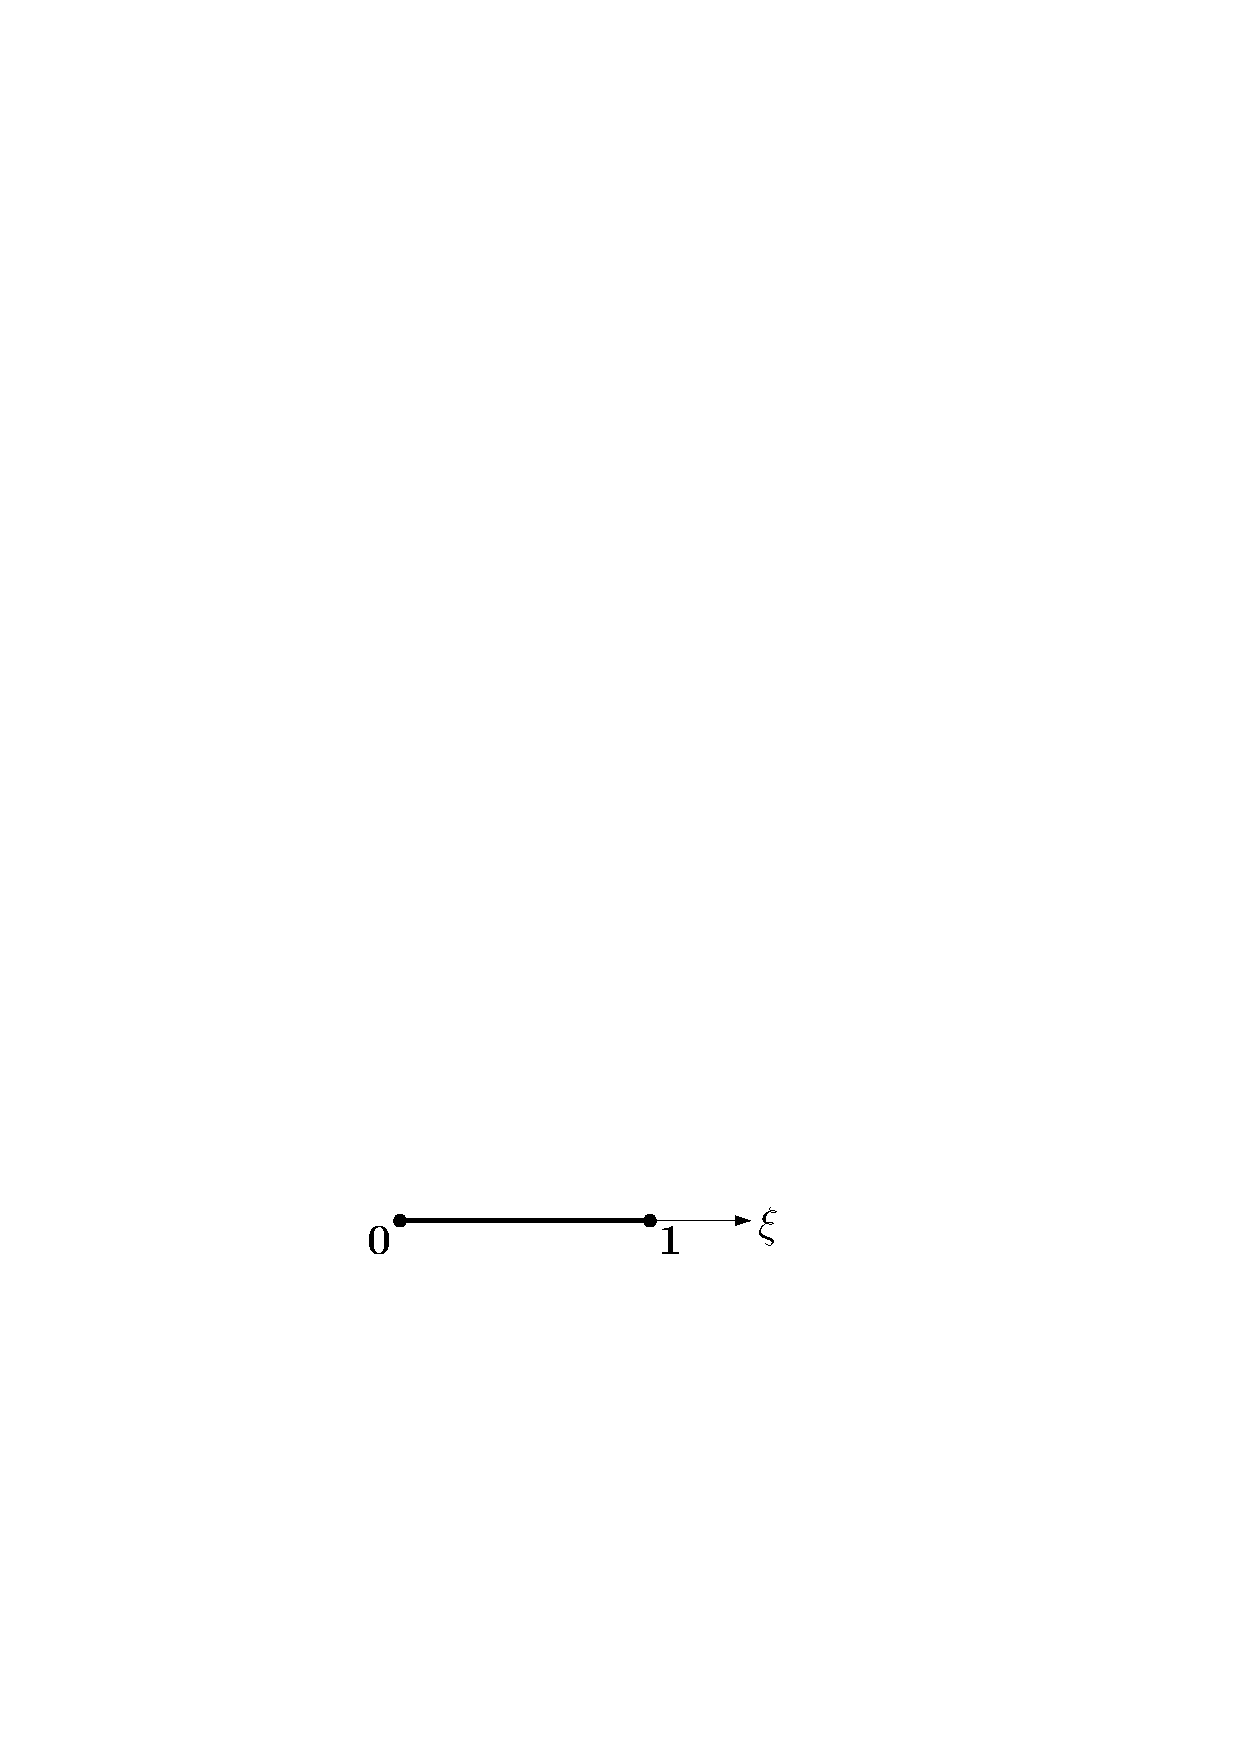
\includegraphics[scale=0.5]{./figures/MasterSegment.pdf}
	\end{center}
\end{minipage}} &\\
\multicolumn{3}{|c|}{Affine Coordinates} &\\
\multicolumn{3}{|c|}{
$	\begin{alignedat}{4}
		\mu_0&=1-\xi\,\qquad\qquad &&\phantom{\nabla}\mu_1&&=\xi\\
		\nabla\mu_0&=-1\,\qquad\qquad &&\nabla\mu_1&&=1
	\end{alignedat}$} &\\
\multicolumn{3}{|c|}{\small\fbox{The order in the pair $\vec{\mu}_{01}=(\mu_0,\mu_1)$ is $p$.}} &\\
\multicolumn{3}{|c|}{} &\\[-17pt]
\hline
\multicolumn{3}{|c|}{$H^1$} &\\
\hline
{}& {} &{} &\\[-23pt]%To keep total width fixed
\multicolumn{2}{|c|}{Shape Functions}& Indices &\\ 
\hline
\multicolumn{2}{|l|}{Vertices} &
\multirow{2}{*}[-12pt]{\small$\begin{gathered}
	a\!=\!0,1
\end{gathered}$} &\\
\multicolumn{2}{|l|}{
$	\begin{aligned}
		\phi^\mathrm{v}&=\mu_a\\
		\nabla\phi^\mathrm{v}&=\nabla\mu_a
	\end{aligned}$} &{}&\\
\multicolumn{2}{|l|}{Edges} &
\multirow{2}{*}[-12pt]{\small$\begin{gathered}
	i\!=\!2,\ldots,p
\end{gathered}$} &\\
\multicolumn{2}{|l|}{
$	\begin{aligned}
		\phi_i^\mathrm{e}&=\phi_i^\E(\vec{\mu}_{01})\,\\
		\nabla\phi_i^\mathrm{e}&=\nabla\phi_i^\E(\vec{\mu}_{01})
	\end{aligned}$} &{}&\\[-17pt]
{}& {} &{} &\\
\hline
\multicolumn{3}{|c|}{$L^2$} &\\
\hline
{}& {} &{} &\\[-23pt]%To keep total width fixed
\multicolumn{2}{|c|}{Shape Functions}& Indices &\\ 
\hline
\multicolumn{2}{|l|}{Edges} &
\multirow{2}{*}[-12pt]{\small$\begin{gathered}
	i\!=\!0,\ldots,p\!-\!1
\end{gathered}$} &\\
\multicolumn{2}{|l|}{
$	\begin{aligned}
		\psi^\mathrm{e}_i=[P_i](\vec{\mu}_{01})\nabla\mu_1
	\end{aligned}$} &{}&\\[-17pt]
{}& {} &{} &\\
\hline
\end{tabular}
\end{center}
\renewcommand{\arraystretch}{1}%Back to normal spacing

\newpage
\subsection{Quadrilateral}

%%%%%%%%%%%%%%%%%%%%%Quadrilateral 1: Geometry,H1%%%%%%%%%%%%%%%%%%%%%
\renewcommand{\arraystretch}{1.35}%Better row spacing
\begin{center}
\begin{tabular}
{|C{0.35cm} L{11.9cm}|C{2.9cm}|N}%See main file for this custom columns - they keep a fixed width while maintaining aligment
\hline
\multicolumn{3}{|c|}{\large \textbf{Quadrilateral}} &\\
\hline
\multicolumn{3}{|c|}{Geometry} &\\
\hline
\multicolumn{3}{|c|}{} &\\[-17pt]
\multicolumn{3}{|c|}{\begin{minipage}{0.9\textwidth}
	\begin{center}
		\includegraphics[scale=0.5]{./figures/MasterQuad.pdf}
	\end{center}
\end{minipage}} &\\
\multicolumn{3}{|c|}{Affine Coordinates} &\\
\multicolumn{3}{|c|}{
$	\begin{alignedat}{4}
		\mu_0^{\,\xi_1}&=1-\xi_1\,\qquad\qquad &&\phantom{\nabla}\mu_1^{\,\xi_1}&&=\xi_1\\
		\nabla\mu_0^{\,\xi_1}&=\Big(\begin{smallmatrix}-1\\[2pt]0\end{smallmatrix}\Big)\qquad\qquad 
			&&\nabla\mu_1^{\,\xi_1}&&=\Big(\begin{smallmatrix}1\\[2pt]0\end{smallmatrix}\Big)\\
		\mu_0^{\,\xi_2}&=1-\xi_2\,\qquad\qquad &&\phantom{\nabla}\mu_1^{\,\xi_2}&&=\xi_2\\
		\nabla\mu_0^{\,\xi_2}&=\Big(\begin{smallmatrix}0\\[2pt]-1\end{smallmatrix}\Big)\qquad\qquad 
			&&\nabla\mu_1^{\,\xi_2}&&=\Big(\begin{smallmatrix}0\\[2pt]1\end{smallmatrix}\Big)
	\end{alignedat}$} &\\
\multicolumn{3}{|c|}{} &\\[-17pt]
\multicolumn{3}{|c|}{\small\fbox{\parbox[c][25pt][c]{0.4\textwidth}{The order in the pair $\vec{\mu}_{01}^{\,\xi_1}=(\mu_0^{\,\xi_1},\mu_1^{\,\xi_1})$ is $p_1$.\\The order in the pair $\vec{\mu}_{01}^{\,\xi_2}=(\mu_0^{\,\xi_2},\mu_1^{\,\xi_2})$ is $p_2$.}}} &\\
\multicolumn{3}{|c|}{} &\\[-17pt]
\hline
\multicolumn{3}{|c|}{$H^1$} &\\
\hline
{}& {} &{} &\\[-23pt]%To keep total width fixed
\multicolumn{2}{|c|}{Shape Functions}& Indices &\\ 
\hline
\multicolumn{2}{|l|}{Vertices} &
\multirow{2}{*}[-12pt]{\small$\begin{gathered}
	a\!=\!0,1,\,b\!=\!0,1
\end{gathered}$} &\\
\multicolumn{2}{|l|}{
$	\begin{aligned}
		\phi^\mathrm{v}&=\mu_a^{\,\xi_1}\mu_b^{\,\xi_2}\\
		\nabla\phi^\mathrm{v}&=\mu_a^{\,\xi_1}\nabla\mu_b^{\,\xi_2}+\mu_b^{\,\xi_2}\nabla\mu_a^{\,\xi_1}
	\end{aligned}$} &{}&\\
\multicolumn{2}{|l|}{Edges} &
\multirow{2}{*}[-12pt]{\small$\begin{gathered}
	i\!=\!2,\ldots,p_a\\
	(a,b)\!=\!(1,2),(2,1)\\
	c\!=\!0,1
\end{gathered}$} &\\
\multicolumn{2}{|l|}{
$	\begin{aligned}
		\phi_i^\mathrm{e}&=\mu_c^{\,\xi_b}\phi_i^\E(\vec{\mu}_{01}^{\,\xi_a})\\
		\nabla\phi_i^\mathrm{e}&=\mu_c^{\,\xi_b}\nabla\phi_i^\E(\vec{\mu}_{01}^{\,\xi_a})
        +\phi_i^\E(\vec{\mu}_{01}^{\,\xi_a})\nabla\mu_c^{\,\xi_b}
	\end{aligned}$} &{}&\\
\multicolumn{2}{|l|}{Face} &
\multirow{2}{*}[-12pt]{\small$\begin{gathered}
	i\!=\!2,\ldots,p_1\\
	j\!=\!2,\ldots,p_2
\end{gathered}$} &\\
\multicolumn{2}{|l|}{
$	\begin{aligned}
		\phi_{ij}^\mathrm{f}&=\phi_{ij}^\square(\vec{\mu}_{01}^{\,\xi_1},\vec{\mu}_{01}^{\,\xi_2})\\
		\nabla\phi_{ij}^\mathrm{f}&=\nabla\phi_{ij}^\square(\vec{\mu}_{01}^{\,\xi_1},\vec{\mu}_{01}^{\,\xi_2})
	\end{aligned}$} &{}&\\[-17pt]
{}& {} &{} &\\[-5pt]
\multicolumn{3}{r}{\footnotesize\textit{continued on next page}} &\\[-18.5pt]
\hline
\end{tabular}
\end{center}
\renewcommand{\arraystretch}{1}%Back to normal spacing

\newpage

%%%%%%%%%%%%%%%%%%%%%Quadrilateral 2: Hcurl,Hdiv%%%%%%%%%%%%%%%%%%%%%
\renewcommand{\arraystretch}{1.35}%Better row spacing
\begin{center}
\begin{tabular}
{|C{0.35cm} L{11.9cm}|C{2.9cm}|N}%See main file for this custom columns - they keep a fixed width while maintaining aligment
\multicolumn{3}{l}{\footnotesize\textit{continued from previous page}} &\\[-2pt]
\hline
\multicolumn{3}{|c|}{\large \textbf{Quadrilateral}} &\\
\hline
\multicolumn{3}{|c|}{$H(\mathrm{curl})^\star$} &\\
\hline
{}& {} &{} &\\[-23pt]%To keep total width fixed
\multicolumn{2}{|c|}{Shape Functions}& Indices &\\ 
\hline
\multicolumn{2}{|l|}{Edges} &
\multirow{2}{*}[-12pt]{\small$\begin{gathered}
	i\!=\!0,\ldots,p_a\!-\!1\\
	(a,b)\!=\!(1,2),(2,1)\\
	c\!=\!0,1
\end{gathered}$} &\\
\multicolumn{2}{|l|}{
$	\begin{aligned}
		E_i^\mathrm{e}&=\mu_c^{\,\xi_b}E_i^\E(\vec{\mu}_{01}^{\,\xi_a})\\
		\nabla\!\times\! E_i^\mathrm{e}&=\nabla\mu_c^{\,\xi_b}\!\times\! E_i^\E(\vec{\mu}_{01}^{\,\xi_a})
	\end{aligned}$} &{}&\\
\multicolumn{2}{|l|}{Face} & {}&\\
\multicolumn{2}{|l|}{\small $\,$Family I} &
\multirow{2}{*}[-12pt]{\small$\begin{gathered}
	i\!=\!0,\ldots,p_1\!-\!1\\
	j\!=\!2,\ldots,p_2
\end{gathered}$} &\\
\multicolumn{2}{|l|}{
$	\begin{aligned}
		E_{ij}^{\mathrm{f}}&=E_{ij}^{\square}(\vec{\mu}_{01}^{\,\xi_1},\vec{\mu}_{01}^{\,\xi_2})\\
		\nabla\!\times\! E_{ij}^{\mathrm{f}}&=\nabla\!\times\! E_{ij}^{\square}(\vec{\mu}_{01}^{\,\xi_1},\vec{\mu}_{01}^{\,\xi_2})
	\end{aligned}$} &{}&\\
\multicolumn{2}{|l|}{\small $\,$Family II} &
\multirow{2}{*}[-12pt]{\small$\begin{gathered}
	i\!=\!0,\ldots,p_2\!-\!1\\
	j\!=\!2,\ldots,p_1
\end{gathered}$} &\\
\multicolumn{2}{|l|}{
$	\begin{aligned}
		E_{ij}^{\mathrm{f}}&=E_{ij}^{\square}(\vec{\mu}_{01}^{\,\xi_2},\vec{\mu}_{01}^{\,\xi_1})\\
		\nabla\!\times\! E_{ij}^{\mathrm{f}}&=\nabla\!\times\! E_{ij}^{\square}(\vec{\mu}_{01}^{\,\xi_2},\vec{\mu}_{01}^{\,\xi_1})
	\end{aligned}$} &{}&\\[-17pt]
{}& {} &{} &\\
\hline
\multicolumn{3}{|c|}{$H(\mathrm{div})$} &\\
\hline
{}& {} &{} &\\[-23pt]%To keep total width fixed
\multicolumn{2}{|c|}{Shape Functions}& Indices &\\ 
\hline
\multicolumn{2}{|l|}{\parbox[c][35pt][l]{0.75\textwidth}{For any given topological entity, the $H(\mathrm{div})$ shape functions are the rotation of the corresponding $H(\mathrm{curl})$ shape functions:}}& {} &\\[30pt]
\multicolumn{2}{|l|}{
$	\begin{aligned}
		V&=\Big(\begin{smallmatrix}0&1\\[2pt]-1&0\end{smallmatrix}\Big)E\\
		\nabla\!\cdot\! V&=\nabla\!\times\! E
	\end{aligned}$} &{}&\\[-17pt]
{}& {} &{} &\\
\hline
\multicolumn{3}{|c|}{$L^2$} &\\
\hline
{}& {} &{} &\\[-23pt]%To keep total width fixed
\multicolumn{2}{|c|}{Shape Functions}& Indices &\\ 
\hline
\multicolumn{2}{|l|}{Face} &
\multirow{2}{*}[-5pt]{\small$\begin{gathered}
	i\!=\!0,\ldots,p_1\!-\!1\\
	j\!=\!0,\ldots,p_2\!-\!1
\end{gathered}$} &\\
\multicolumn{2}{|l|}{
$	\begin{aligned}
		\psi_{ij}^\mathrm{f}=[P_i](\vec{\mu}_{01}^{\,\xi_1})[P_j](\vec{\mu}_{01}^{\,\xi_2})
			(\nabla\mu_1^{\,\xi_1}\!\times\!\nabla\mu_1^{\,\xi_2})
	\end{aligned}$} &{}&\\[-4pt]
\multicolumn{3}{|c|}{} &\\[-11.25pt]
\multicolumn{3}{|c|}{} &\\[-47.75pt]
{}& {} &{} &\\
\hline
\multicolumn{3}{r}{} &\\[-18.5pt]
\multicolumn{3}{l}{\multirow{1}{*}[4pt]{\footnotesize $\star$ In 2D the curl and cross product are $\nabla\!\times\!\Big(\begin{smallmatrix}E_1\\[2pt]E_2\end{smallmatrix}\Big)
        =\frac{\partial E_2}{\partial \xi_1}-\frac{\partial E_1}{\partial \xi_2}$ and $\Big(\begin{smallmatrix}E_1\\[2pt]E_2\end{smallmatrix}\Big)\!\times\!\Big(\begin{smallmatrix}F_1\\[2pt]F_2\end{smallmatrix}\Big)=E_1F_2-E_2F_1$ respectively.}} &\\[-8.5pt]
\multicolumn{3}{r}{} &\\[-18.5pt]
\hline
\end{tabular}
\end{center}
\renewcommand{\arraystretch}{1}%Back to normal spacing

\newpage
\subsection{Triangle}

%%%%%%%%%%%%%%%%%%%%%Triangle 1: Geometry,H1%%%%%%%%%%%%%%%%%%%%%
\renewcommand{\arraystretch}{1.35}%Better row spacing
\begin{center}
\begin{tabular}
{|C{0.35cm} L{11.9cm}|C{2.9cm}|N}%See main file for this custom columns - they keep a fixed width while maintaining aligment
\hline
\multicolumn{3}{|c|}{\large \textbf{Triangle}} &\\
\hline
\multicolumn{3}{|c|}{Geometry} &\\
\hline
\multicolumn{3}{|c|}{} &\\[-17pt]
\multicolumn{3}{|c|}{\begin{minipage}{0.9\textwidth}
	\begin{center}
		\includegraphics[scale=0.5]{./figures/MasterTri.pdf}
	\end{center}
\end{minipage}} &\\
\multicolumn{3}{|c|}{Affine Coordinates} &\\
\multicolumn{3}{|c|}{
$	\begin{alignedat}{6}
		\nu_0&=1-x_1-x_2\,\qquad\qquad &&\phantom{\nabla}\nu_1&&=x_1\qquad\qquad &&\phantom{\nabla}\nu_2&&=x_2\\
		\nabla\nu_0&=\Big(\begin{smallmatrix}-1\\[2pt]-1\end{smallmatrix}\Big)\qquad\qquad 
			&&\nabla\nu_1&&=\Big(\begin{smallmatrix}1\\[2pt]0\end{smallmatrix}\Big)\qquad\qquad 
				&&\nabla\nu_2&&=\Big(\begin{smallmatrix}0\\[2pt]1\end{smallmatrix}\Big)
	\end{alignedat}$} &\\
\multicolumn{3}{|c|}{} &\\[-17pt]
\multicolumn{3}{|c|}{\small\fbox{The order in the triplet $\vec{\nu}_{012}=(\nu_0,\nu_1,\nu_2)$ and all its subpairs is $p$.}} &\\
\multicolumn{3}{|c|}{} &\\[-17pt]
\hline
\multicolumn{3}{|c|}{$H^1$} &\\
\hline
{}& {} &{} &\\[-23pt]%To keep total width fixed
\multicolumn{2}{|c|}{Shape Functions}& Indices &\\ 
\hline
\multicolumn{2}{|l|}{Vertices} &
\multirow{2}{*}[-12pt]{\small$\begin{gathered}
	a\!=\!0,1,2
\end{gathered}$} &\\
\multicolumn{2}{|l|}{
$	\begin{aligned}
		\phi^\mathrm{v}&=\nu_a\\
		\nabla\phi^\mathrm{v}&=\nabla\nu_a
	\end{aligned}$} &{}&\\
\multicolumn{2}{|l|}{Edges} &
\multirow{2}{*}[-12pt]{\small$\begin{gathered}
	i\!=\!2,\ldots,p\\
	0\leq a<b\leq2
\end{gathered}$} &\\
\multicolumn{2}{|l|}{
$	\begin{aligned}
		\phi_i^\mathrm{e}&=\phi_i^\E(\vec{\nu}_{ab})\\
		\nabla\phi_i^\mathrm{e}&=\nabla\phi_i^\E(\vec{\nu}_{ab})
	\end{aligned}$} &{}&\\
\multicolumn{2}{|l|}{Face} &
\multirow{2}{*}[-12pt]{\small$\begin{gathered}
	i\geq2,\,j\geq1\\
	i\!+\!j\!=\!3,\ldots,p
\end{gathered}$} &\\
\multicolumn{2}{|l|}{
$	\begin{aligned}
		\phi_{ij}^\mathrm{f}&=\phi_{ij}^\Tri(\vec{\nu}_{012})\\
		\nabla\phi_{ij}^\mathrm{f}&=\nabla\phi_{ij}^\Tri(\vec{\nu}_{012})
	\end{aligned}$} &{}&\\[-17pt]
{}& {} &{} &\\[-5pt]
\multicolumn{3}{r}{\footnotesize\textit{continued on next page}} &\\[-18.5pt]
\hline
\end{tabular}
\end{center}
\renewcommand{\arraystretch}{1}%Back to normal spacing

\newpage

%%%%%%%%%%%%%%%%%%%%%Triangle 2: Hcurl,Hdiv%%%%%%%%%%%%%%%%%%%%%
\renewcommand{\arraystretch}{1.35}%Better row spacing
\begin{center}
\begin{tabular}
{|C{0.35cm} L{11.9cm}|C{2.9cm}|N}%See main file for this custom columns - they keep a fixed width while maintaining aligment
\multicolumn{3}{l}{\footnotesize\textit{continued from previous page}} &\\[-2pt]
\hline
\multicolumn{3}{|c|}{\large \textbf{Triangle}} &\\
\hline
\multicolumn{3}{|c|}{$H(\mathrm{curl})^\star$} &\\
\hline
{}& {} &{} &\\[-23pt]%To keep total width fixed
\multicolumn{2}{|c|}{Shape Functions}& Indices &\\ 
\hline
\multicolumn{2}{|l|}{Edges} &
\multirow{2}{*}[-12pt]{\small$\begin{gathered}
	i\!=\!0,\ldots,p\!-\!1\\
	0\leq a<b\leq2
\end{gathered}$} &\\
\multicolumn{2}{|l|}{
$	\begin{aligned}
		E_i^\mathrm{e}&=E_i^\E(\vec{\nu}_{ab})\\
		\nabla\!\times\! E_i^\mathrm{e}&=\nabla\!\times\! E_i^\E(\vec{\nu}_{ab})
	\end{aligned}$} &{}&\\
\multicolumn{2}{|l|}{Face} & {}&\\
\multicolumn{2}{|l|}{\small $\,$Family I} &
\multirow{2}{*}[-12pt]{\small$\begin{gathered}
	i\geq0,\,j\geq1\\
	i\!+\!j\!=\!1,\ldots,p\!-\!1
\end{gathered}$} &\\
\multicolumn{2}{|l|}{
$	\begin{aligned}
		E_{ij}^{\mathrm{f}}&=E_{ij}^\Tri(\vec{\nu}_{012})\\
		\nabla\!\times\! E_{ij}^{\mathrm{f}}&=\nabla\!\times\! E_{ij}^\Tri(\vec{\nu}_{012})
	\end{aligned}$} &{}&\\
\multicolumn{2}{|l|}{\small $\,$Family II} &
\multirow{2}{*}[-12pt]{\small$\begin{gathered}
	i\geq0,\,j\geq1\\
	i\!+\!j\!=\!1,\ldots,p\!-\!1
\end{gathered}$} &\\
\multicolumn{2}{|l|}{
$	\begin{aligned}
		E_{ij}^{\mathrm{f}}&=E_{ij}^\Tri(\vec{\nu}_{120})\\
		\nabla\!\times\! E_{ij}^{\mathrm{f}}&=\nabla\!\times\! E_{ij}^\Tri(\vec{\nu}_{120})
	\end{aligned}$} &{}&\\[-17pt]
{}& {} &{} &\\
\hline
\multicolumn{3}{|c|}{$H(\mathrm{div})$} &\\
\hline
{}& {} &{} &\\[-23pt]%To keep total width fixed
\multicolumn{2}{|c|}{Shape Functions}& Indices &\\ 
\hline
\multicolumn{2}{|l|}{\parbox[c][35pt][l]{0.75\textwidth}{For any given topological entity, the $H(\mathrm{div})$ shape functions are the rotation of the corresponding $H(\mathrm{curl})$ shape functions:}}& {} &\\[30pt]
\multicolumn{2}{|l|}{
$	\begin{aligned}
		V&=\Big(\begin{smallmatrix}0&1\\[2pt]-1&0\end{smallmatrix}\Big)E\\
		\nabla\!\cdot\! V&=\nabla\!\times\! E
	\end{aligned}$} &{}&\\[-17pt]
{}& {} &{} &\\
\hline
\multicolumn{3}{|c|}{$L^2$} &\\
\hline
{}& {} &{} &\\[-23pt]%To keep total width fixed
\multicolumn{2}{|c|}{Shape Functions}& Indices &\\ 
\hline
\multicolumn{2}{|l|}{Face} &
\multirow{2}{*}[-5pt]{\small$\begin{gathered}
	i\geq0,\,j\geq0\\
	i\!+\!j\!=\!0,\ldots,p\!-\!1
\end{gathered}$} &\\
\multicolumn{2}{|l|}{
$	\begin{aligned}
		\psi_{ij}^\mathrm{f}=[P_i](\vec{\nu}_{01})[P_j^{2i+1}](\nu_0+\nu_1,\nu_2)
			(\nabla\nu_1\!\times\!\nabla\nu_2)
	\end{aligned}$} &{}&\\[-4pt]
\multicolumn{3}{|c|}{} &\\[-11.25pt]
\multicolumn{3}{|c|}{} &\\[-47.75pt]
{}& {} &{} &\\
\hline
\multicolumn{3}{r}{} &\\[-18.5pt]
\multicolumn{3}{l}{\multirow{1}{*}[4pt]{\footnotesize $\star$ In 2D the curl and cross product are $\nabla\!\times\!\Big(\begin{smallmatrix}E_1\\[2pt]E_2\end{smallmatrix}\Big)
        =\frac{\partial E_2}{\partial x_1}-\frac{\partial E_1}{\partial x_2}$ and $\Big(\begin{smallmatrix}E_1\\[2pt]E_2\end{smallmatrix}\Big)\!\times\!\Big(\begin{smallmatrix}F_1\\[2pt]F_2\end{smallmatrix}\Big)=E_1F_2-E_2F_1$ respectively.}} &\\[-8.5pt]
\multicolumn{3}{r}{} &\\[-18.5pt]
\hline
\end{tabular}
\end{center}
\renewcommand{\arraystretch}{1}%Back to normal spacing

\newpage
\subsection{Hexahedron}

%%%%%%%%%%%%%%%%%%%%%Hexahedron 1: Geometry%%%%%%%%%%%%%%%%%%%%%
\renewcommand{\arraystretch}{1.35}%Better row spacing
\begin{center}
\begin{tabular}
{|C{0.35cm} L{11.9cm} C{2.9cm}|N}%See main file for this custom columns - they keep a fixed width while maintaining aligment
\hline
\multicolumn{3}{|c|}{\large \textbf{Hexahedron}} &\\
\hline
\multicolumn{3}{|c|}{Geometry} &\\
\hline
\multicolumn{3}{|c|}{} &\\[-10pt]
\multicolumn{3}{|c|}{\begin{minipage}{0.9\textwidth}
	\begin{center}
		\includegraphics[scale=0.5]{./figures/MasterHexa.pdf}
	\end{center}
\end{minipage}} &\\
\multicolumn{3}{|c|}{Affine Coordinates} &\\
\multicolumn{3}{|c|}{
$	\begin{alignedat}{4}
		\mu_0^{\,\xi_1}&=1-\xi_1\,\qquad\qquad &&\phantom{\nabla}\mu_1^{\,\xi_1}&&=\xi_1\\
		\nabla\mu_0^{\,\xi_1}&=\bigg(\begin{smallmatrix}-1\\[2pt]0\\[2pt]0\end{smallmatrix}\bigg)\qquad\qquad 
			&&\nabla\mu_1^{\,\xi_1}&&=\bigg(\begin{smallmatrix}1\\[2pt]0\\[2pt]0\end{smallmatrix}\bigg)\\
		\mu_0^{\,\xi_2}&=1-\xi_2\,\qquad\qquad &&\phantom{\nabla}\mu_1^{\,\xi_2}&&=\xi_2\\
		\nabla\mu_0^{\,\xi_2}&=\bigg(\begin{smallmatrix}0\\[2pt]-1\\[2pt]0\end{smallmatrix}\bigg)\qquad\qquad 
			&&\nabla\mu_1^{\,\xi_2}&&=\bigg(\begin{smallmatrix}0\\[2pt]1\\[2pt]0\end{smallmatrix}\bigg)\\
		\mu_0^{\,\xi_3}&=1-\xi_3\,\qquad\qquad &&\phantom{\nabla}\mu_1^{\,\xi_3}&&=\xi_3\\
		\nabla\mu_0^{\,\xi_3}&=\bigg(\begin{smallmatrix}0\\[2pt]0\\[2pt]-1\end{smallmatrix}\bigg)\qquad\qquad 
			&&\nabla\mu_1^{\,\xi_3}&&=\bigg(\begin{smallmatrix}0\\[2pt]0\\[2pt]1\end{smallmatrix}\bigg)
	\end{alignedat}$} &\\
\multicolumn{3}{|c|}{} &\\[-7pt]
\multicolumn{3}{|c|}{\small\fbox{\parbox[c][40pt][c]{0.4\textwidth}{The order in the pair $\vec{\mu}_{01}^{\,\xi_1}=(\mu_0^{\,\xi_1},\mu_1^{\,\xi_1})$ is $p_1$.\\The order in the pair $\vec{\mu}_{01}^{\,\xi_2}=(\mu_0^{\,\xi_2},\mu_1^{\,\xi_2})$ is $p_2$.\\The order in the pair $\vec{\mu}_{01}^{\,\xi_3}=(\mu_0^{\,\xi_3},\mu_1^{\,\xi_3})$ is $p_3$.}}} &\\
\multicolumn{3}{|c|}{} &\\[-17pt]
{}& {} &{} &\\[-5pt]
\multicolumn{3}{r}{\footnotesize\textit{continued on next page}} &\\[-18.5pt]
\hline
\end{tabular}
\end{center}
\renewcommand{\arraystretch}{1}%Back to normal spacing

\newpage

%%%%%%%%%%%%%%%%%%%%%Hexahedron 2: H1%%%%%%%%%%%%%%%%%%%%%
\renewcommand{\arraystretch}{1.35}%Better row spacing
\begin{center}
\begin{tabular}
{|C{0.35cm} L{11.9cm}|C{2.9cm}|N}%See main file for this custom columns - they keep a fixed width while maintaining aligment
\multicolumn{3}{l}{\footnotesize\textit{continued from previous page}} &\\[-2pt]
\hline
\multicolumn{3}{|c|}{\large \textbf{Hexahedron}} &\\
\hline
\multicolumn{3}{|c|}{$H^1$} &\\
\hline
{}& {} &{} &\\[-23pt]%To keep total width fixed
\multicolumn{2}{|c|}{Shape Functions}& Indices &\\ 
\hline
\multicolumn{2}{|l|}{Vertices} &
\multirow{2}{*}[-12pt]{\small$\begin{gathered}
	a\!=\!0,1,\,b\!=\!0,1\\
	c\!=\!0,1
\end{gathered}$} &\\
\multicolumn{2}{|l|}{
$	\begin{aligned}
		\phi^\mathrm{v}&=\mu_a^{\,\xi_1}\mu_b^{\,\xi_2}\mu_c^{\,\xi_3}\\
		\nabla\phi^\mathrm{v}&=\mu_a^{\,\xi_1}\mu_b^{\,\xi_2}\nabla\mu_c^{\,\xi_3}+\mu_c^{\,\xi_3}\mu_a^{\,\xi_1}\nabla\mu_b^{\,\xi_2}
			+\mu_b^{\,\xi_2}\mu_c^{\,\xi_3}\nabla\mu_a^{\,\xi_1}
	\end{aligned}$} &{}&\\
\multicolumn{2}{|l|}{Edges} &
\multirow{2}{*}[-12pt]{\small$\begin{gathered}
	i\!=\!2,\ldots,p_a\\[-2pt]
	(a,b,c)\!=\!(1,2,3),\\[-2pt]
	(2,3,1),(3,1,2)\\[-2pt]
	d\!=\!0,1,\,e\!=\!0,1,
\end{gathered}$} &\\
\multicolumn{2}{|l|}{
$	\begin{aligned}
		\phi_i^\mathrm{e}&=\mu_e^{\,\xi_c}\mu_d^{\,\xi_b}\phi_i^\E(\vec{\mu}_{01}^{\,\xi_a})\\
		\nabla\phi_i^\mathrm{e}&=\mu_e^{\,\xi_c}\mu_d^{\,\xi_b}\nabla\phi_i^\E(\vec{\mu}_{01}^{\,\xi_a})
			+\phi_i^\E(\vec{\mu}_{01}^{\,\xi_a})\Big(\mu_e^{\,\xi_c}\nabla\mu_d^{\,\xi_b}+\mu_d^{\,\xi_b}\nabla\mu_e^{\,\xi_c}\Big)
	\end{aligned}$} &{}&\\[30pt]
\multicolumn{2}{|l|}{Faces} &
\multirow{2}{*}[-9pt]{\small$\begin{gathered}
	i\!=\!2,\ldots,p_a\\[-2pt]
	j\!=\!2,\ldots,p_b\\[-2pt]
	(a,b,c)\!=\!(1,2,3),\\[-2pt]
	(2,3,1),(3,1,2)\\[-2pt]
	d\!=\!0,1
\end{gathered}$} &\\
\multicolumn{2}{|l|}{
$	\begin{aligned}
		\phi_{ij}^\mathrm{f}&=\mu_d^{\,\xi_c}\phi_{ij}^\square(\vec{\mu}_{01}^{\,\xi_a},\vec{\mu}_{01}^{\,\xi_b})\\
		\nabla\phi_{ij}^\mathrm{f}&=\mu_d^{\,\xi_c}\nabla\phi_{ij}^\square(\vec{\mu}_{01}^{\,\xi_a},\vec{\mu}_{01}^{\,\xi_b})
			+\phi_{ij}^\square(\vec{\mu}_{01}^{\,\xi_a},\vec{\mu}_{01}^{\,\xi_b})\nabla\mu_d^{\,\xi_c}
	\end{aligned}$} &{}&\\[35pt]
\multicolumn{2}{|l|}{Interior} &
\multirow{2}{*}[-12pt]{\small$\begin{gathered}
	i\!=\!2,\ldots,p_1\\[-2pt]
	j\!=\!2,\ldots,p_2\\[-2pt]
	k\!=\!2,\ldots,p_3
\end{gathered}$} &\\
\multicolumn{2}{|l|}{
$	\begin{aligned}
		\phi_{ijk}^\mathrm{b}&=\phi_{ij}^\square(\vec{\mu}_{01}^{\,\xi_1},\vec{\mu}_{01}^{\,\xi_2})\phi_k^\E(\vec{\mu}_{01}^{\,\xi_3})\\
		\nabla\phi_{ijk}^\mathrm{b}&=
			\phi_{ij}^\square(\vec{\mu}_{01}^{\,\xi_1},\vec{\mu}_{01}^{\,\xi_2})\nabla\phi_k^\E(\vec{\mu}_{01}^{\,\xi_3})
				+\phi_k^\E(\vec{\mu}_{01}^{\,\xi_3})\nabla\phi_{ij}^\square(\vec{\mu}_{01}^{\,\xi_1},\vec{\mu}_{01}^{\,\xi_2})
	\end{aligned}$} &{}&\\[-15pt]
{}& {} &{} &\\[-5pt]
\multicolumn{3}{r}{\footnotesize\textit{continued on next page}} &\\[-18.5pt]
\hline
\end{tabular}
\end{center}
\renewcommand{\arraystretch}{1}%Back to normal spacing

\newpage

%%%%%%%%%%%%%%%%%%%%%Hexahedron 3: Hcurl%%%%%%%%%%%%%%%%%%%%%
\renewcommand{\arraystretch}{1.35}%Better row spacing
\begin{center}
\begin{tabular}
{|C{0.35cm} L{11.9cm}|C{2.9cm}|N}%See main file for this custom columns - they keep a fixed width while maintaining aligment
\multicolumn{3}{l}{\footnotesize\textit{continued from previous page}} &\\[-2pt]
\hline
\multicolumn{3}{|c|}{\large \textbf{Hexahedron}} &\\
\hline
\multicolumn{3}{|c|}{$H(\mathrm{curl})$} &\\
\hline
{}& {} &{} &\\[-23pt]%To keep total width fixed
\multicolumn{2}{|c|}{Shape Functions}& Indices &\\ 
\hline
\multicolumn{2}{|l|}{Edges} &
\multirow{2}{*}[-12pt]{\small$\begin{gathered}
	i\!=\!0,\ldots,p_a\!-\!1\\[-2pt]
	(a,b,c)\!=\!(1,2,3),\\[-2pt]
	(2,3,1),(3,1,2)\\[-2pt]
	d\!=\!0,1,\,e\!=\!0,1,
\end{gathered}$} &\\
\multicolumn{2}{|l|}{
$	\begin{aligned}
		E_i^\mathrm{e}&=\mu_e^{\,\xi_c}\mu_d^{\,\xi_b}E_i^\E(\vec{\mu}_{01}^{\,\xi_a})\\
		\nabla\!\times\! E_i^\mathrm{e}&=\Big(\mu_e^{\,\xi_c}\nabla\mu_d^{\,\xi_b}+\mu_d^{\,\xi_b}\nabla\mu_e^{\,\xi_c}\Big)
			\!\times\! E_i^\E(\vec{\mu}_{01}^{\,\xi_a})
	\end{aligned}$} &{}&\\[25pt]
\multicolumn{2}{|l|}{Faces} & {}&\\[-5pt]
\multicolumn{2}{|l|}{\small $\,$Family I} &
\multirow{2}{*}[-12pt]{\small$\begin{gathered}
	i\!=\!0,\ldots,p_a\!-\!1\\[-2pt]
	j\!=\!2,\ldots,p_b\\[-2pt]
	(a,b,c)\!=\!(1,2,3),\\[-2pt]
	(2,3,1),(3,1,2)\\[-2pt]
	d\!=\!0,1
\end{gathered}$} &\\
\multicolumn{2}{|l|}{
$	\begin{aligned}
		E_{ij}^{\mathrm{f}}&=\mu_d^{\,\xi_c}E_{ij}^\square(\vec{\mu}_{01}^{\,\xi_a},\vec{\mu}_{01}^{\,\xi_b})\\
		\nabla\!\times\! E_{ij}^{\mathrm{f}}&=\mu_d^{\,\xi_c}
			\nabla\!\times\! E_{ij}^\square(\vec{\mu}_{01}^{\,\xi_a},\vec{\mu}_{01}^{\,\xi_b})
				+\nabla\mu_d^{\,\xi_c}\!\times\! E_{ij}^\square(\vec{\mu}_{01}^{\,\xi_a},\vec{\mu}_{01}^{\,\xi_b})
	\end{aligned}$} &{}&\\[35pt]
\multicolumn{2}{|l|}{\small $\,$Family II} &
\multirow{2}{*}[-12pt]{\small$\begin{gathered}
	i\!=\!0,\ldots,p_b\!-\!1\\[-2pt]
	j\!=\!2,\ldots,p_a\\[-2pt]
	(a,b,c)\!=\!(1,2,3),\\[-2pt]
	(2,3,1),(3,1,2)\\[-2pt]
	d\!=\!0,1
\end{gathered}$} &\\
\multicolumn{2}{|l|}{
$	\begin{aligned}
		E_{ij}^{\mathrm{f}}&=\mu_d^{\,\xi_c}E_{ij}^\square(\vec{\mu}_{01}^{\,\xi_b},\vec{\mu}_{01}^{\,\xi_a})\\
		\nabla\!\times\! E_{ij}^{\mathrm{f}}&=\mu_d^{\,\xi_c}
			\nabla\!\times\! E_{ij}^\square(\vec{\mu}_{01}^{\,\xi_b},\vec{\mu}_{01}^{\,\xi_a})
				+\nabla\mu_d^{\,\xi_c}\!\times\! E_{ij}^\square(\vec{\mu}_{01}^{\,\xi_b},\vec{\mu}_{01}^{\,\xi_a})
	\end{aligned}$} &{}&\\[35pt]
\multicolumn{2}{|l|}{Interior} & {}&\\[-5pt]
\multicolumn{2}{|l|}{\small $\,$Family I} &
\multirow{2}{*}[-12pt]{\small$\begin{gathered}
	i\!=\!0,\ldots,p_1\!-\!1\\[-2pt]
	j\!=\!2,\ldots,p_2\\[-2pt]
	k\!=\!2,\ldots,p_3
\end{gathered}$} &\\
\multicolumn{2}{|l|}{
$	\begin{aligned}
		E_{ijk}^\mathrm{b}&=\phi_k^\E(\vec{\mu}_{01}^{\,\xi_3})E_{ij}^\square(\vec{\mu}_{01}^{\,\xi_1},\vec{\mu}_{01}^{\,\xi_2})\\
		\nabla\!\times\! E_{ijk}^\mathrm{b}&=\phi_k^\E(\vec{\mu}_{01}^{\,\xi_3})\nabla\!\times\!
			E_{ij}^\square(\vec{\mu}_{01}^{\,\xi_1},\vec{\mu}_{01}^{\,\xi_2})
				+\nabla\phi_k^\E(\vec{\mu}_{01}^{\,\xi_3})\!\times\! E_{ij}^\square(\vec{\mu}_{01}^{\,\xi_1},\vec{\mu}_{01}^{\,\xi_2})
	\end{aligned}$} &{}&\\
\multicolumn{2}{|l|}{\small $\,$Family II} &
\multirow{2}{*}[-12pt]{\small$\begin{gathered}
	i\!=\!0,\ldots,p_2\!-\!1\\[-2pt]
	j\!=\!2,\ldots,p_3\\[-2pt]
	k\!=\!2,\ldots,p_1
\end{gathered}$} &\\
\multicolumn{2}{|l|}{
$	\begin{aligned}
		E_{ijk}^\mathrm{b}&=\phi_k^\E(\vec{\mu}_{01}^{\,\xi_1})E_{ij}^\square(\vec{\mu}_{01}^{\,\xi_2},\vec{\mu}_{01}^{\,\xi_3})\\
		\nabla\!\times\! E_{ijk}^\mathrm{b}&=\phi_k^\E(\vec{\mu}_{01}^{\,\xi_1})\nabla\!\times\!
			E_{ij}^\square(\vec{\mu}_{01}^{\,\xi_2},\vec{\mu}_{01}^{\,\xi_3})
				+\nabla\phi_k^\E(\vec{\mu}_{01}^{\,\xi_1})\!\times\! E_{ij}^\square(\vec{\mu}_{01}^{\,\xi_2},\vec{\mu}_{01}^{\,\xi_3})
	\end{aligned}$} &{}&\\
\multicolumn{2}{|l|}{\small $\,$Family III} &
\multirow{2}{*}[-12pt]{\small$\begin{gathered}
	i\!=\!0,\ldots,p_3\!-\!1\\[-2pt]
	j\!=\!2,\ldots,p_1\\[-2pt]
	k\!=\!2,\ldots,p_2
\end{gathered}$} &\\
\multicolumn{2}{|l|}{
$	\begin{aligned}
		E_{ijk}^\mathrm{b}&=\phi_k^\E(\vec{\mu}_{01}^{\,\xi_2})E_{ij}^\square(\vec{\mu}_{01}^{\,\xi_3},\vec{\mu}_{01}^{\,\xi_1})\\
		\nabla\!\times\! E_{ijk}^\mathrm{b}&=\phi_k^\E(\vec{\mu}_{01}^{\,\xi_2})\nabla\!\times\!
			E_{ij}^\square(\vec{\mu}_{01}^{\,\xi_3},\vec{\mu}_{01}^{\,\xi_1})
				+\nabla\phi_k^\E(\vec{\mu}_{01}^{\,\xi_2})\!\times\! E_{ij}^\square(\vec{\mu}_{01}^{\,\xi_3},\vec{\mu}_{01}^{\,\xi_1})
	\end{aligned}$} &{}&\\[-17pt]
{}& {} &{} &\\[-5pt]
\multicolumn{3}{r}{\footnotesize\textit{continued on next page}} &\\[-18.5pt]
\hline
\end{tabular}
\end{center}
\renewcommand{\arraystretch}{1}%Back to normal spacing

\newpage

%%%%%%%%%%%%%%%%%%%%%Hexahedron 4: Hdiv,L2%%%%%%%%%%%%%%%%%%%%%
\renewcommand{\arraystretch}{1.35}%Better row spacing
\begin{center}
\begin{tabular}
{|C{0.35cm} L{11.9cm}|C{2.9cm}|N}%See main file for this custom columns - they keep a fixed width while maintaining aligment
\multicolumn{3}{l}{\footnotesize\textit{continued from previous page}} &\\[-2pt]
\hline
\multicolumn{3}{|c|}{\large \textbf{Hexahedron}} &\\
\hline
\multicolumn{3}{|c|}{$H(\mathrm{div})$} &\\
\hline
{}& {} &{} &\\[-23pt]%To keep total width fixed
\multicolumn{2}{|c|}{Shape Functions}& Indices &\\ 
\hline
\multicolumn{2}{|l|}{Faces} & 
\multirow{2}{*}[-12pt]{\small$\begin{gathered}
	i\!=\!0,\ldots,p_a\!-\!1\\[-2pt]
	j\!=\!0,\ldots,p_b\!-\!1\\[-2pt]
	(a,b,c)\!=\!(1,2,3),\\[-2pt]
	(2,3,1),(3,1,2)\\[-2pt]
	d\!=\!0,1
\end{gathered}$} &\\
\multicolumn{2}{|l|}{
$	\begin{aligned}
		V_{ij}^\mathrm{f}&=\mu_d^{\,\xi_c}V_{ij}^{\square}(\vec{\mu}_{01}^{\,\xi_a},\vec{\mu}_{01}^{\,\xi_b})\\
		\nabla\!\cdot\! V_{ij}^\mathrm{f}&=
			\nabla\mu_d^{\,\xi_c}\!\cdot\! V_{ij}^{\square}(\vec{\mu}_{01}^{\,\xi_a},\vec{\mu}_{01}^{\,\xi_b})
	\end{aligned}$} &{}&\\[35pt]
\multicolumn{2}{|l|}{Interior} & {}&\\[-5pt]
\multicolumn{2}{|l|}{\small $\,$Family I} &
\multirow{2}{*}[-12pt]{\small$\begin{gathered}
	i\!=\!0,\ldots,p_1\!-\!1\\[-2pt]
	j\!=\!0,\ldots,p_2\!-\!1\\[-2pt]
	k\!=\!2,\ldots,p_3
\end{gathered}$} &\\
\multicolumn{2}{|l|}{
$	\begin{aligned}
		V_{ijk}^\mathrm{b}&=\phi_k^\E(\vec{\mu}_{01}^{\,\xi_3})V_{ij}^\square(\vec{\mu}_{01}^{\,\xi_1},\vec{\mu}_{01}^{\,\xi_2})\\
		\nabla\!\cdot\! V_{ijk}^\mathrm{b}&=
			\nabla\phi_k^\E(\vec{\mu}_{01}^{\,\xi_3})\!\cdot\! V_{ij}^\square(\vec{\mu}_{01}^{\,\xi_1},\vec{\mu}_{01}^{\,\xi_2})
	\end{aligned}$} &{}&\\
\multicolumn{2}{|l|}{\small $\,$Family II} &
\multirow{2}{*}[-12pt]{\small$\begin{gathered}
	i\!=\!0,\ldots,p_2\!-\!1\\[-2pt]
	j\!=\!0,\ldots,p_3\!-\!1\\[-2pt]
	k\!=\!2,\ldots,p_1
\end{gathered}$} &\\
\multicolumn{2}{|l|}{
$	\begin{aligned}
		V_{ijk}^\mathrm{b}&=\phi_k^\E(\vec{\mu}_{01}^{\,\xi_1})V_{ij}^\square(\vec{\mu}_{01}^{\,\xi_2},\vec{\mu}_{01}^{\,\xi_3})\\
		\nabla\!\cdot\! V_{ijk}^\mathrm{b}&=
			\nabla\phi_k^\E(\vec{\mu}_{01}^{\,\xi_1})\!\cdot\! V_{ij}^\square(\vec{\mu}_{01}^{\,\xi_2},\vec{\mu}_{01}^{\,\xi_3})
	\end{aligned}$} &{}&\\
\multicolumn{2}{|l|}{\small $\,$Family III} &
\multirow{2}{*}[-12pt]{\small$\begin{gathered}
	i\!=\!0,\ldots,p_3\!-\!1\\[-2pt]
	j\!=\!0,\ldots,p_1\!-\!1\\[-2pt]
	k\!=\!2,\ldots,p_2
\end{gathered}$} &\\
\multicolumn{2}{|l|}{
$	\begin{aligned}
		V_{ijk}^\mathrm{b}&=\phi_k^\E(\vec{\mu}_{01}^{\,\xi_2})V_{ij}^\square(\vec{\mu}_{01}^{\,\xi_3},\vec{\mu}_{01}^{\,\xi_1})\\
		\nabla\!\cdot\! V_{ijk}^\mathrm{b}&=
			\nabla\phi_k^\E(\vec{\mu}_{01}^{\,\xi_2})\!\cdot\! V_{ij}^\square(\vec{\mu}_{01}^{\,\xi_3},\vec{\mu}_{01}^{\,\xi_1})
	\end{aligned}$} &{}&\\[-17pt]
{}& {} &{} &\\
\hline
\multicolumn{3}{|c|}{$L^2$} &\\
\hline
{}& {} &{} &\\[-23pt]%To keep total width fixed
\multicolumn{2}{|c|}{Shape Functions}& Indices &\\ 
\hline
\multicolumn{2}{|l|}{Interior} &
\multirow{2}{*}[-5pt]{\small$\begin{gathered}
	i\!=\!0,\ldots,p_1\!-\!1\\
	j\!=\!0,\ldots,p_2\!-\!1\\
	k\!=\!0,\ldots,p_3\!-\!1
\end{gathered}$} &\\
\multicolumn{2}{|l|}{
$	\begin{aligned}
		\psi_{ijk}^\mathrm{b}=[P_i](\vec{\mu}_{01}^{\,\xi_1})[P_j](\vec{\mu}_{01}^{\,\xi_2})[P_k](\vec{\mu}_{01}^{\,\xi_3})
			(\nabla\mu_1^{\,\xi_1}\!\times\!\nabla\mu_1^{\,\xi_2})\!\cdot\!\nabla\mu_1^{\,\xi_3}
	\end{aligned}$} &{}&\\[-10pt]
{}& {} &{} &\\
\hline
\end{tabular}
\end{center}
\renewcommand{\arraystretch}{1}%Back to normal spacing


\newpage
\subsection{Tetrahedron}

%%%%%%%%%%%%%%%%%%%%%Tetrahedron 1: Geometry%%%%%%%%%%%%%%%%%%%%%
\renewcommand{\arraystretch}{1.35}%Better row spacing
\begin{center}
\begin{tabular}
{|C{0.35cm} L{11.9cm} C{2.9cm}|N}%See main file for this custom columns - they keep a fixed width while maintaining aligment
\hline
\multicolumn{3}{|c|}{\large \textbf{Tetrahedron}} &\\
\hline
\multicolumn{3}{|c|}{Geometry} &\\
\hline
\multicolumn{3}{|c|}{} &\\[-10pt]
\multicolumn{3}{|c|}{\begin{minipage}{0.9\textwidth}
	\begin{center}
		\includegraphics[scale=0.5]{./figures/MasterTet.pdf}
	\end{center}
\end{minipage}} &\\
\multicolumn{3}{|c|}{Affine Coordinates} &\\
\multicolumn{3}{|c|}{
$	\begin{alignedat}{8}
		\lambda_0&=1-x_1-x_2-x_3\qquad\quad&&\phantom{\nabla}\lambda_1&&=x_1\qquad\quad
			&&\phantom{\nabla}\lambda_2&&=x_2\qquad\quad&&\phantom{\nabla}\lambda_3&&=x_3\\
		\nabla\lambda_0&=\bigg(\begin{smallmatrix}-1\\[2pt]-1\\[2pt]-1\end{smallmatrix}\bigg)\qquad\quad 
			&&\nabla\lambda_1&&=\bigg(\begin{smallmatrix}1\\[2pt]0\\[2pt]0\end{smallmatrix}\bigg)\qquad\quad 
				&&\nabla\lambda_2&&=\bigg(\begin{smallmatrix}0\\[2pt]1\\[2pt]0\end{smallmatrix}\bigg)\qquad\quad
					&&\nabla\lambda_3&&=\bigg(\begin{smallmatrix}0\\[2pt]0\\[2pt]1\end{smallmatrix}\bigg)
	\end{alignedat}$} &\\
\multicolumn{3}{|c|}{} &\\[-8pt]
\multicolumn{3}{|c|}{\small\fbox{The order in the quadruple $\vec{\lambda}_{0123}=(\lambda_0,\lambda_1,\lambda_2,\lambda_3)$ and all its subtuples is $p$.}} &\\[-5pt]
{}& {} &{} &\\[-5pt]
\multicolumn{3}{r}{\footnotesize\textit{continued on next page}} &\\[-18.5pt]
\hline
\end{tabular}
\end{center}
\renewcommand{\arraystretch}{1}%Back to normal spacing

\newpage

%%%%%%%%%%%%%%%%%%%%%Tetrahedron 2: H1%%%%%%%%%%%%%%%%%%%%%
\renewcommand{\arraystretch}{1.35}%Better row spacing
\begin{center}
\begin{tabular}
{|C{0.35cm} L{11.9cm}|C{2.9cm}|N}%See main file for this custom columns - they keep a fixed width while maintaining aligment
\multicolumn{3}{l}{\footnotesize\textit{continued from previous page}} &\\[-2pt]
\hline
\multicolumn{3}{|c|}{\large \textbf{Tetrahedron}} &\\
\hline
\multicolumn{3}{|c|}{$H^1$} &\\
\hline
{}& {} &{} &\\[-23pt]%To keep total width fixed
\multicolumn{2}{|c|}{Shape Functions}& Indices &\\ 
\hline
\multicolumn{2}{|l|}{Vertices} &
\multirow{2}{*}[-12pt]{\small$\begin{gathered}
	a\!=\!0,1,2,3
\end{gathered}$} &\\
\multicolumn{2}{|l|}{
$	\begin{aligned}
		\phi^\mathrm{v}&=\lambda_a\\
		\nabla\phi^\mathrm{v}&=\nabla\lambda_a
	\end{aligned}$} &{}&\\
\multicolumn{2}{|l|}{Edges} &
\multirow{2}{*}[-12pt]{\small$\begin{gathered}
	i\!=\!2,\ldots,p\\
	0\leq a<b\leq3
\end{gathered}$} &\\
\multicolumn{2}{|l|}{
$	\begin{aligned}
		\phi_i^\mathrm{e}&=\phi_i^\E(\vec{\lambda}_{ab})\\
		\nabla\phi_i^\mathrm{e}&=\nabla\phi_i^\E(\vec{\lambda}_{ab})
	\end{aligned}$} &{}&\\
\multicolumn{2}{|l|}{Faces} &
\multirow{2}{*}[-12pt]{\small$\begin{gathered}
	i\geq2,\,j\geq1\\
	i\!+\!j\!=\!3,\ldots,p\\
	0\leq a<b<c\leq3	
\end{gathered}$} &\\
\multicolumn{2}{|l|}{
$	\begin{aligned}
		\phi_{ij}^\mathrm{f}&=\phi_{ij}^\Tri(\vec{\lambda}_{abc})\\
		\nabla\phi_{ij}^\mathrm{f}&=\nabla\phi_{ij}^\Tri(\vec{\lambda}_{abc})
	\end{aligned}$} &{}&\\
\multicolumn{2}{|l|}{Interior} &
\multirow{2}{*}[-12pt]{\small$\begin{gathered}
	i\geq2,\,j\geq1,\,k\geq1\\
	i\!+\!j\!+\!k\!=\!4,\ldots,p
\end{gathered}$} &\\[-5pt]
\multicolumn{2}{|l|}{
$	\begin{aligned}
		\phi_{ijk}^\mathrm{b}&=\phi_{ij}^\Tri(\vec{\lambda}_{012})[L_k^{2(i+j)}](1\!-\!\lambda_3,\lambda_3)\\
		\nabla\phi_{ijk}^\mathrm{b}&=
			[L_k^{2(i+j)}](1\!-\!\lambda_3,\lambda_3)\nabla\phi_{ij}^\Tri(\vec{\lambda}_{012})
				+\phi_{ij}^\Tri(\vec{\lambda}_{012})\nabla[L_k^{2(i+j)}](1\!-\!\lambda_3,\lambda_3)
	\end{aligned}$} &{}&\\[-15pt]
{}& {} &{} &\\[-5pt]
\multicolumn{3}{r}{\footnotesize\textit{continued on next page}} &\\[-18.5pt]
\hline
\end{tabular}
\end{center}
\renewcommand{\arraystretch}{1}%Back to normal spacing

\newpage

%%%%%%%%%%%%%%%%%%%%%Tetrahedron 3: Hcurl%%%%%%%%%%%%%%%%%%%%%
\renewcommand{\arraystretch}{1.35}%Better row spacing
\begin{center}
\begin{tabular}
{|C{0.35cm} L{11.9cm}|C{2.9cm}|N}%See main file for this custom columns - they keep a fixed width while maintaining aligment
\multicolumn{3}{l}{\footnotesize\textit{continued from previous page}} &\\[-2pt]
\hline
\multicolumn{3}{|c|}{\large \textbf{Tetrahedron}} &\\
\hline
\multicolumn{3}{|c|}{$H(\mathrm{curl})$} &\\
\hline
{}& {} &{} &\\[-23pt]%To keep total width fixed
\multicolumn{2}{|c|}{Shape Functions}& Indices &\\ 
\hline
\multicolumn{2}{|l|}{Edges} &
\multirow{2}{*}[-12pt]{\small$\begin{gathered}
	i\!=\!0,\ldots,p\!-\!1\\
	0\leq a<b\leq3
\end{gathered}$} &\\
\multicolumn{2}{|l|}{
$	\begin{aligned}
		E_i^\mathrm{e}&=E_i^\E(\vec{\lambda}_{ab})\\
		\nabla\!\times\! E_i^\mathrm{e}&=\nabla\times E_i^\E(\vec{\lambda}_{ab})
	\end{aligned}$} &{}&\\
\multicolumn{2}{|l|}{Faces} & {}&\\[-5pt]
\multicolumn{2}{|l|}{\small $\,$Family I} &
\multirow{2}{*}[-12pt]{\small$\begin{gathered}
	i\geq0,\,j\geq1\\[-2pt]
	i\!+\!j\!=\!1,\ldots,p\!-\!1\\[-2pt]
	0\leq a<b<c\leq3
\end{gathered}$} &\\
\multicolumn{2}{|l|}{
$	\begin{aligned}
		E_{ij}^{\mathrm{f}}&=E_{ij}^\Tri(\vec{\lambda}_{abc})\\
		\nabla\!\times\! E_{ij}^{\mathrm{f}}&=\nabla\!\times\!E_{ij}^\Tri(\vec{\lambda}_{abc})
	\end{aligned}$} &{}&\\
\multicolumn{2}{|l|}{\small $\,$Family II} &
\multirow{2}{*}[-12pt]{\small$\begin{gathered}
	i\geq0,\,j\geq1\\[-2pt]
	i\!+\!j\!=\!1,\ldots,p\!-\!1\\[-2pt]
	0\leq a<b<c\leq3
\end{gathered}$} &\\
\multicolumn{2}{|l|}{
$	\begin{aligned}
		E_{ij}^{\mathrm{f}}&=E_{ij}^\Tri(\vec{\lambda}_{bca})\\
		\nabla\!\times\! E_{ij}^{\mathrm{f}}&=\nabla\!\times\!E_{ij}^\Tri(\vec{\lambda}_{bca})
	\end{aligned}$} &{}&\\
\multicolumn{2}{|l|}{Interior} & {}&\\[-10pt]
\multicolumn{2}{|l|}{\small $\,$Family I} &
\multirow{2}{*}[-12pt]{\small$\begin{gathered}
	i\geq0,\,j\geq1,\,k\geq1\\
	i\!\!+\!\!j\!\!+\!\!k\!=\!2,\ldots,p\!\!-\!\!1
\end{gathered}$} &\\[-5pt]
\multicolumn{2}{|l|}{
$	\begin{aligned}
		E_{ijk}^\mathrm{b}&=[L_k^{2(i+j)}](1\!\!-\!\!\lambda_3,\lambda_3)E_{ij}^\Tri(\vec{\lambda}_{012})\\
		\nabla\!\times\! E_{ijk}^\mathrm{b}&=[L_k^{2(i+j)}](1\!\!-\!\!\lambda_3,\lambda_3)
			\nabla\!\!\times\!\! E_{ij}^\Tri(\vec{\lambda}_{012})
				\!+\!\nabla[L_k^{2(i+j)}](1\!\!-\!\!\lambda_3,\lambda_3)\!\times\! E_{ij}^\Tri(\vec{\lambda}_{012})
	\end{aligned}$} &{}&\\
\multicolumn{2}{|l|}{\small $\,$Family II} &
\multirow{2}{*}[-12pt]{\small$\begin{gathered}
	i\geq0,\,j\geq1,\,k\geq1\\
	i\!\!+\!\!j\!\!+\!\!k\!=\!2,\ldots,p\!\!-\!\!1
\end{gathered}$} &\\[-5pt]
\multicolumn{2}{|l|}{
$	\begin{aligned}
		E_{ijk}^\mathrm{b}&=[L_k^{2(i+j)}](1\!\!-\!\!\lambda_0,\lambda_0)E_{ij}^\Tri(\vec{\lambda}_{123})\\
		\nabla\!\times\! E_{ijk}^\mathrm{b}&=[L_k^{2(i+j)}](1\!\!-\!\!\lambda_0,\lambda_0)
			\nabla\!\!\times\!\! E_{ij}^\Tri(\vec{\lambda}_{123})
				\!+\!\nabla[L_k^{2(i+j)}](1\!\!-\!\!\lambda_0,\lambda_0)\!\times\! E_{ij}^\Tri(\vec{\lambda}_{123})	
	\end{aligned}$} &{}&\\
\multicolumn{2}{|l|}{\small $\,$Family III} &
\multirow{2}{*}[-12pt]{\small$\begin{gathered}
	i\geq0,\,j\geq1,\,k\geq1\\
	i\!\!+\!\!j\!\!+\!\!k\!=\!2,\ldots,p\!\!-\!\!1
\end{gathered}$} &\\[-5pt]
\multicolumn{2}{|l|}{
$	\begin{aligned}
		E_{ijk}^\mathrm{b}&=[L_k^{2(i+j)}](1\!\!-\!\!\lambda_1,\lambda_1)E_{ij}^\Tri(\vec{\lambda}_{230})\\
		\nabla\!\times\! E_{ijk}^\mathrm{b}&=[L_k^{2(i+j)}](1\!\!-\!\!\lambda_1,\lambda_1)
			\nabla\!\!\times\!\! E_{ij}^\Tri(\vec{\lambda}_{230})
				\!+\!\nabla[L_k^{2(i+j)}](1\!\!-\!\!\lambda_1,\lambda_1)\!\times\! E_{ij}^\Tri(\vec{\lambda}_{230})
	\end{aligned}$} &{}&\\[-17pt]
{}& {} &{} &\\[-5pt]
\multicolumn{3}{r}{\footnotesize\textit{continued on next page}} &\\[-18.5pt]
\hline
\end{tabular}
\end{center}
\renewcommand{\arraystretch}{1}%Back to normal spacing

\newpage

%%%%%%%%%%%%%%%%%%%%%Tetrahedron 4: Hdiv,L2%%%%%%%%%%%%%%%%%%%%%
\renewcommand{\arraystretch}{1.35}%Better row spacing
\begin{center}
\begin{tabular}
{|C{0.35cm} L{11.9cm}|C{2.9cm}|N}%See main file for this custom columns - they keep a fixed width while maintaining aligment
\multicolumn{3}{l}{\footnotesize\textit{continued from previous page}} &\\[-2pt]
\hline
\multicolumn{3}{|c|}{\large \textbf{Tetrahedron}} &\\
\hline
\multicolumn{3}{|c|}{$H(\mathrm{div})$} &\\
\hline
{}& {} &{} &\\[-23pt]%To keep total width fixed
\multicolumn{2}{|c|}{Shape Functions}& Indices &\\ 
\hline
\multicolumn{2}{|l|}{Faces} & 
\multirow{2}{*}[-12pt]{\small$\begin{gathered}
	i\geq0,\,j\geq0\\[-2pt]
	i\!+\!j\!=\!0,\ldots,p\!-\!1\\[-2pt]
	0\leq a<b<c\leq3
\end{gathered}$} &\\
\multicolumn{2}{|l|}{
$	\begin{aligned}
		V_{ij}^\mathrm{f}&=V_{ij}^\Tri(\vec{\lambda}_{abc})\\
		\nabla\!\cdot\! V_{ij}^\mathrm{f}&=\nabla\!\cdot\! V_{ij}^\Tri(\vec{\lambda}_{abc}(x))
	\end{aligned}$} &{}&\\
\multicolumn{2}{|l|}{Interior} & {}&\\[-10pt]
\multicolumn{2}{|l|}{\small $\,$Family I} &
\multirow{2}{*}[-12pt]{\small$\begin{gathered}
	i\geq0,\,j\geq0,\,k\geq1\\
	i\!\!+\!\!j\!\!+\!\!k\!=\!1,\ldots,p\!\!-\!\!1
\end{gathered}$} &\\[-5pt]
\multicolumn{2}{|l|}{
$	\begin{aligned}
		V_{ijk}^\mathrm{b}&=[L_k^{2(i\!+\!j\!+\!1)}](1\!\!-\!\!\lambda_3,\lambda_3)V_{ij}^\Tri(\vec{\lambda}_{012})\\
		\nabla\!\cdot\! V_{ijk}^\mathrm{b}&=
			[L_k^{2(i\!+\!j\!+\!1)}](1\!\!-\!\!\lambda_3,\lambda_3)\nabla\!\cdot\! V_{ij}^\Tri(\vec{\lambda}_{012})
				\!+\!\nabla[L_k^{2(i\!+\!j\!+\!1)}](1\!\!-\!\!\lambda_3,\lambda_3)\!\cdot\! V_{ij}^\Tri(\vec{\lambda}_{012})
	\end{aligned}$} &{}&\\
\multicolumn{2}{|l|}{\small $\,$Family II} &
\multirow{2}{*}[-12pt]{\small$\begin{gathered}
	i\geq0,\,j\geq0,\,k\geq1\\
	i\!\!+\!\!j\!\!+\!\!k\!=\!1,\ldots,p\!\!-\!\!1
\end{gathered}$} &\\[-5pt]
\multicolumn{2}{|l|}{
$	\begin{aligned}
		V_{ijk}^\mathrm{b}&=[L_k^{2(i\!+\!j\!+\!1)}](1\!\!-\!\!\lambda_0,\lambda_0)V_{ij}^\Tri(\vec{\lambda}_{123})\\
		\nabla\!\cdot\! V_{ijk}^\mathrm{b}&=
			[L_k^{2(i\!+\!j\!+\!1)}](1\!\!-\!\!\lambda_0,\lambda_0)\nabla\!\cdot\! V_{ij}^\Tri(\vec{\lambda}_{123})
				\!+\!\nabla[L_k^{2(i\!+\!j\!+\!1)}](1\!\!-\!\!\lambda_0,\lambda_0)\!\cdot\! V_{ij}^\Tri(\vec{\lambda}_{123})
	\end{aligned}$} &{}&\\
\multicolumn{2}{|l|}{\small $\,$Family III} &
\multirow{2}{*}[-12pt]{\small$\begin{gathered}
	i\geq0,\,j\geq0,\,k\geq1\\
	i\!\!+\!\!j\!\!+\!\!k\!=\!1,\ldots,p\!\!-\!\!1
\end{gathered}$} &\\[-5pt]
\multicolumn{2}{|l|}{
$	\begin{aligned}
		V_{ijk}^\mathrm{b}&=[L_k^{2(i\!+\!j\!+\!1)}](1\!\!-\!\!\lambda_1,\lambda_1)V_{ij}^\Tri(\vec{\lambda}_{230})\\
		\nabla\!\cdot\! V_{ijk}^\mathrm{b}&=
			[L_k^{2(i\!+\!j\!+\!1)}](1\!\!-\!\!\lambda_1,\lambda_1)\nabla\!\cdot\! V_{ij}^\Tri(\vec{\lambda}_{230})
				\!+\!\nabla[L_k^{2(i\!+\!j\!+\!1)}](1\!\!-\!\!\lambda_1,\lambda_1)\!\cdot\! V_{ij}^\Tri(\vec{\lambda}_{230})
	\end{aligned}$} &{}&\\[-17pt]
{}& {} &{} &\\
\hline
\multicolumn{3}{|c|}{$L^2$} &\\
\hline
{}& {} &{} &\\[-23pt]%To keep total width fixed
\multicolumn{2}{|c|}{Shape Functions}& Indices &\\ 
\hline
\multicolumn{2}{|l|}{Interior} &
\multirow{2}{*}[2pt]{\small$\begin{gathered}
	i\geq0,\,j\geq0,\,k\geq0\\
	i\!\!+\!\!j\!\!+\!\!k\!=\!0,\ldots,p\!\!-\!\!1
\end{gathered}$} &\\[-10pt]
\multicolumn{2}{|l|}{
$	\begin{aligned}
		\psi_{ijk}^\mathrm{b}=[P_i](\vec{\lambda}_{01})[P_j^{2i\!+\!1}](\lambda_0\!+\!\lambda_1,\lambda_2)
			[P_k^{2(i\!+\!j\!+\!1)}](1\!-\!\lambda_3,\lambda_3)(\nabla\lambda_1\!\times\!\nabla\lambda_2)\!\cdot\!\nabla\lambda_3
	\end{aligned}$} &{}&\\[-17pt]
{}& {} &{} &\\
\hline
\end{tabular}
\end{center}
\renewcommand{\arraystretch}{1}%Back to normal spacing


\newpage
\subsection{Prism}

%%%%%%%%%%%%%%%%%%%%%Prism 1: Geometry%%%%%%%%%%%%%%%%%%%%%
\renewcommand{\arraystretch}{1.35}%Better row spacing
\begin{center}
\begin{tabular}
{|C{0.35cm} L{11.9cm} C{2.9cm}|N}%See main file for this custom columns - they keep a fixed width while maintaining aligment
\hline
\multicolumn{3}{|c|}{\large \textbf{Prism}} &\\
\hline
\multicolumn{3}{|c|}{Geometry} &\\
\hline
\multicolumn{3}{|c|}{} &\\[-10pt]
\multicolumn{3}{|c|}{\begin{minipage}{0.9\textwidth}
	\begin{center}
		\includegraphics[scale=0.5]{./figures/MasterPrismTables.pdf}
	\end{center}
\end{minipage}} &\\
\multicolumn{3}{|c|}{Affine Coordinates} &\\
\multicolumn{3}{|c|}{
$	\begin{alignedat}{6}
		\nu_0&=1-x_1-x_2\,\qquad\qquad &&\phantom{\nabla}\nu_1&&=x_1\qquad\qquad &&\phantom{\nabla}\nu_2&&=x_2\\
		\nabla\nu_0&=\bigg(\begin{smallmatrix}-1\\[2pt]-1\\[2pt]0\end{smallmatrix}\bigg)\qquad\qquad 
			&&\nabla\nu_1&&=\bigg(\begin{smallmatrix}1\\[2pt]0\\[2pt]0\end{smallmatrix}\bigg)\qquad\qquad 
				&&\nabla\nu_2&&=\bigg(\begin{smallmatrix}0\\[2pt]1\\[2pt]0\end{smallmatrix}\bigg)
	\end{alignedat}$} &\\[30pt]
\multicolumn{3}{|c|}{
$	\begin{alignedat}{4}
		\mu_0&=1-z\,\qquad\qquad &&\phantom{\nabla}\mu_1&&=z\\
		\nabla\mu_0&=\bigg(\begin{smallmatrix}0\\[2pt]0\\[2pt]-1\end{smallmatrix}\bigg)\qquad\qquad 
			&&\nabla\mu_1&&=\bigg(\begin{smallmatrix}0\\[2pt]0\\[2pt]1\end{smallmatrix}\bigg)
	\end{alignedat}$} &\\
\multicolumn{3}{|c|}{} &\\[-8pt]
\multicolumn{3}{|c|}{\small\fbox{\parbox[c][25pt][c]{0.6\textwidth}{The order in the triplet $\vec{\nu}_{012}=(\nu_0,\nu_1,\nu_2)$ and all its subpairs is $p$.\\The order in the pair $\vec{\mu}_{01}=(\mu_0,\mu_1)$ is $q$.}}} &\\
{}& {} &{} &\\[-5pt]
\multicolumn{3}{r}{\footnotesize\textit{continued on next page}} &\\[-18.5pt]
\hline
\end{tabular}
\end{center}
\renewcommand{\arraystretch}{1}%Back to normal spacing

\newpage

%%%%%%%%%%%%%%%%%%%%%Prism 2: H1%%%%%%%%%%%%%%%%%%%%%
\renewcommand{\arraystretch}{1.35}%Better row spacing
\begin{center}
\begin{tabular}
{|C{0.35cm} L{11.9cm}|C{2.9cm}|N}%See main file for this custom columns - they keep a fixed width while maintaining aligment
\multicolumn{3}{l}{\footnotesize\textit{continued from previous page}} &\\[-2pt]
\hline
\multicolumn{3}{|c|}{\large \textbf{Prism}} &\\
\hline
\multicolumn{3}{|c|}{$H^1$} &\\
\hline
{}& {} &{} &\\[-23pt]%To keep total width fixed
\multicolumn{2}{|c|}{Shape Functions}& Indices &\\ 
\hline
\multicolumn{2}{|l|}{Vertices} &
\multirow{2}{*}[-12pt]{\small$\begin{gathered}
	a\!=\!0,1,2\\
	c\!=\!0,1
\end{gathered}$} &\\
\multicolumn{2}{|l|}{
$	\begin{aligned}
		\phi^\mathrm{v}&=\nu_a\mu_c\\
		\nabla\phi^\mathrm{v}&=\mu_c\nabla\nu_a+\nu_a\nabla\mu_c
	\end{aligned}$} &{}&\\
\multicolumn{2}{|l|}{Mixed Edges} &
\multirow{2}{*}[-10pt]{\small$\begin{gathered}
	i\!=\!2,\ldots,p\\[-2pt]
	0\leq a<b\leq2\\[-2pt]
	c\!=\!0,1
\end{gathered}$} &\\
\multicolumn{2}{|l|}{
$	\begin{aligned}
		\phi_i^\mathrm{e}&=\mu_c\phi_i^\E(\vec{\nu}_{ab})\\
		\nabla\phi_i^\mathrm{e}&=\mu_c\nabla\phi_i^\E(\vec{\nu}_{ab})+\phi_i^\E(\vec{\nu}_{ab})\nabla\mu_c
	\end{aligned}$} &{}&\\
\multicolumn{2}{|l|}{Quadrilateral Edges} &
\multirow{2}{*}[-10pt]{\small$\begin{gathered}
	i\!=\!2,\ldots,q\\
	a=0,1,2
\end{gathered}$} &\\
\multicolumn{2}{|l|}{
$	\begin{aligned}
		\phi_i^\mathrm{e}&=\nu_a\phi_i^\E(\vec{\mu}_{01})\\
		\nabla\phi_i^\mathrm{e}&=\nu_a\nabla\phi_i^\E(\vec{\mu}_{01})+\phi_i^\E(\vec{\mu}_{01})\nabla\nu_a
	\end{aligned}$} &{}&\\
\multicolumn{2}{|l|}{Triangle Faces} &
\multirow{2}{*}[-12pt]{\small$\begin{gathered}
	i\geq2,\,j\geq1\\[-2pt]
	i\!+\!j\!=\!3,\ldots,p\\[-2pt]
	c\!=\!0,1	
\end{gathered}$} &\\
\multicolumn{2}{|l|}{
$	\begin{aligned}
		\phi_{ij}^\mathrm{f}&=\mu_c\phi_{ij}^\Tri(\vec{\nu}_{012})\\
		\nabla\phi_{ij}^\mathrm{f}&=\mu_c\nabla\phi_{ij}^\Tri(\vec{\nu}_{012})+\phi_{ij}^\Tri(\vec{\nu}_{012})\nabla\mu_c
	\end{aligned}$} &{}&\\
\multicolumn{2}{|l|}{Quadrilateral Faces} &
\multirow{2}{*}[-12pt]{\small$\begin{gathered}
	i\!=\!2,\ldots,p\\[-2pt]
	j\!=\!2,\ldots,q\\[-2pt]
	0\leq a<b\leq2	
\end{gathered}$} &\\
\multicolumn{2}{|l|}{
$	\begin{aligned}
		\phi_{ij}^\mathrm{f}&=\phi_{ij}^\square(\vec{\nu}_{ab},\vec{\mu}_{01})\\
		\nabla\phi_{ij}^\mathrm{f}&=\nabla\phi_{ij}^\square(\vec{\nu}_{ab},\vec{\mu}_{01})
	\end{aligned}$} &{}&\\
\multicolumn{2}{|l|}{Interior} &
\multirow{2}{*}[-12pt]{\small$\begin{gathered}
	i\geq2,\,j\geq1\\[-2pt]
	i\!+\!j\!=\!3,\ldots,p\\[-2pt]
	k\!=\!2,\ldots,q
\end{gathered}$} &\\
\multicolumn{2}{|l|}{
$	\begin{aligned}
		\phi_{ijk}^\mathrm{b}&=\phi_{ij}^\Tri(\vec{\nu}_{012})\phi_k^\E(\vec{\mu}_{01})\\
		\nabla\phi_{ijk}^\mathrm{b}&=\phi_k^\E(\vec{\mu}_{01})\nabla\phi_{ij}^\Tri(\vec{\nu}_{012})
			+\phi_{ij}^\Tri(\vec{\nu}_{012})\nabla\phi_k^\E(\vec{\mu}_{01})
	\end{aligned}$} &{}&\\[-15pt]
{}& {} &{} &\\[-5pt]
\multicolumn{3}{r}{\footnotesize\textit{continued on next page}} &\\[-18.5pt]
\hline
\end{tabular}
\end{center}
\renewcommand{\arraystretch}{1}%Back to normal spacing

\newpage

%%%%%%%%%%%%%%%%%%%%%Prism 3: Hcurl%%%%%%%%%%%%%%%%%%%%%
\renewcommand{\arraystretch}{1.35}%Better row spacing
\begin{center}
\begin{tabular}
{|C{0.35cm} L{11.9cm}|C{2.9cm}|N}%See main file for this custom columns - they keep a fixed width while maintaining aligment
\multicolumn{3}{l}{\footnotesize\textit{continued from previous page}} &\\[-2pt]
\hline
\multicolumn{3}{|c|}{\large \textbf{Prism}} &\\
\hline
\multicolumn{3}{|c|}{$H(\mathrm{curl})$} &\\
\hline
{}& {} &{} &\\[-23pt]%To keep total width fixed
\multicolumn{2}{|c|}{Shape Functions}& Indices &\\ 
\hline
\multicolumn{2}{|l|}{Mixed Edges} &
\multirow{2}{*}[-10pt]{\small$\begin{gathered}
	i\!=\!0,\ldots,p\!-\!1\\[-2pt]
	0\leq a<b\leq2\\[-2pt]
	c\!=\!0,1
\end{gathered}$} &\\
\multicolumn{2}{|l|}{
$	\begin{aligned}
		E_i^\mathrm{e}&=\mu_cE_i^\E(\vec{\nu}_{ab})\\
		\nabla\!\times\! E_i^\mathrm{e}&=\mu_c\nabla\!\times\! E_i^\E(\vec{\nu}_{ab})+\nabla\mu_c\!\times\! E_i^\E(\vec{\nu}_{ab})
	\end{aligned}$} &{}&\\
\multicolumn{2}{|l|}{Quadrilateral Edges} &
\multirow{2}{*}[-10pt]{\small$\begin{gathered}
	i\!=\!0,\ldots,q\!-\!1\\
	a=0,1,2
\end{gathered}$} &\\
\multicolumn{2}{|l|}{
$	\begin{aligned}
		E_i^\mathrm{e}&=\nu_aE_i^\E(\vec{\mu}_{01})\\
		\nabla\!\times\! E_i^\mathrm{e}&=\nabla\nu_a\!\times\! E_i^\E(\vec{\mu}_{01})
	\end{aligned}$} &{}&\\
\multicolumn{2}{|l|}{Triangle Faces} & {}&\\[-5pt]
\multicolumn{2}{|l|}{\small $\,$Family I} &
\multirow{2}{*}[-12pt]{\small$\begin{gathered}
	i\geq0,\,j\geq1\\[-2pt]
	i\!+\!j\!=\!1,\ldots,p\!-\!1\\[-2pt]
	c\!=\!0,1
\end{gathered}$} &\\
\multicolumn{2}{|l|}{
$	\begin{aligned}
		E_{ij}^{\mathrm{f}}&=\mu_cE_{ij}^\Tri(\vec{\nu}_{012})\\
		\nabla\!\times\! E_{ij}^{\mathrm{f}}&=\mu_c\nabla\!\times\! E_{ij}^\Tri(\vec{\nu}_{012})
			+\nabla\mu_c\!\times\! E_{ij}^\Tri(\vec{\nu}_{012})
	\end{aligned}$} &{}&\\
\multicolumn{2}{|l|}{\small $\,$Family II} &
\multirow{2}{*}[-12pt]{\small$\begin{gathered}
	i\geq0,\,j\geq1\\[-2pt]
	i\!+\!j\!=\!1,\ldots,p\!-\!1\\[-2pt]
	c\!=\!0,1
\end{gathered}$} &\\
\multicolumn{2}{|l|}{
$	\begin{aligned}
		E_{ij}^{\mathrm{f}}&=\mu_cE_{ij}^\Tri(\vec{\nu}_{120})\\
		\nabla\!\times\! E_{ij}^{\mathrm{f}}&=\mu_c\nabla\!\times\! E_{ij}^\Tri(\vec{\nu}_{120})
			+\nabla\mu_c\!\times\! E_{ij}^\Tri(\vec{\nu}_{120})
	\end{aligned}$} &{}&\\
\multicolumn{2}{|l|}{Quadrilateral Faces} & {}&\\[-5pt]
\multicolumn{2}{|l|}{\small $\,$Family I} &
\multirow{2}{*}[-12pt]{\small$\begin{gathered}
	i\!=\!0,\ldots,p\!-\!1\\[-2pt]
	j\!=\!2,\ldots,q\\[-2pt]
	0\leq a<b\leq2
\end{gathered}$} &\\
\multicolumn{2}{|l|}{
$	\begin{aligned}
		E_{ij}^{\mathrm{f}}&=E_{ij}^\square(\vec{\nu}_{ab},\vec{\mu}_{01})\\
		\nabla\!\times\! E_{ij}^{\mathrm{f}}&=\nabla\!\times\! E_{ij}^\square(\vec{\nu}_{ab},\vec{\mu}_{01})
	\end{aligned}$} &{}&\\
\multicolumn{2}{|l|}{\small $\,$Family II} &
\multirow{2}{*}[-12pt]{\small$\begin{gathered}
	i\!=\!0,\ldots,q\!-\!1\\[-2pt]
	j\!=\!2,\ldots,p\\[-2pt]
	0\leq a<b\leq2
\end{gathered}$} &\\
\multicolumn{2}{|l|}{
$	\begin{aligned}
		E_{ij}^{\mathrm{f}}&=E_{ij}^\square(\vec{\mu}_{01},\vec{\nu}_{ab})\\
		\nabla\!\times\! E_{ij}^{\mathrm{f}}&=\nabla\!\times\! E_{ij}^\square(\vec{\mu}_{01},\vec{\nu}_{ab})
	\end{aligned}$} &{}&\\[-13pt]
{}& {} &{} &\\[-5pt]
\multicolumn{3}{r}{\footnotesize\textit{continued on next page}} &\\[-18.5pt]
\hline
\end{tabular}
\end{center}
\renewcommand{\arraystretch}{1}%Back to normal spacing

\newpage

%%%%%%%%%%%%%%%%%%%%%Prism 4: Hcurl Interior%%%%%%%%%%%%%%%%%%%%%
\renewcommand{\arraystretch}{1.35}%Better row spacing
\begin{center}
\begin{tabular}
{|C{0.35cm} L{11.9cm}|C{2.9cm}|N}%See main file for this custom columns - they keep a fixed width while maintaining aligment
\multicolumn{3}{l}{\footnotesize\textit{continued from previous page}} &\\[-2pt]
\hline
\multicolumn{3}{|c|}{\large \textbf{Prism}} &\\
\hline
\multicolumn{3}{|c|}{$H(\mathrm{curl})$} &\\
\hline
{}& {} &{} &\\[-23pt]%To keep total width fixed
\multicolumn{2}{|c|}{Shape Functions}& Indices &\\ 
\hline
\multicolumn{2}{|l|}{Interior} & {}&\\[-5pt]
\multicolumn{2}{|l|}{\small $\,$Family I} &
\multirow{2}{*}[-12pt]{\small$\begin{gathered}
	i\geq0,\,j\geq1\\[-2pt]
	i\!+\!j\!=\!1,\ldots,p\!-\!1\\[-2pt]
	k\!=\!2,\ldots,q
\end{gathered}$} &\\
\multicolumn{2}{|l|}{
$	\begin{aligned}
		E_{ijk}^\mathrm{b}&=\phi_k^\E(\vec{\mu}_{01})E_{ij}^\Tri(\vec{\nu}_{012})\\
		\nabla\!\times\! E_{ijk}^\mathrm{b}&=\phi_k^\E(\vec{\mu}_{01})\nabla\!\times\! E_{ij}^\Tri(\vec{\nu}_{012})
			+\nabla\phi_k^\E(\vec{\mu}_{01})\!\times\! E_{ij}^\Tri(\vec{\nu}_{012})
	\end{aligned}$} &{}&\\
\multicolumn{2}{|l|}{\small $\,$Family II} &
\multirow{2}{*}[-12pt]{\small$\begin{gathered}
	i\geq0,\,j\geq1\\[-2pt]
	i\!+\!j\!=\!1,\ldots,p\!-\!1\\[-2pt]
	k\!=\!2,\ldots,q
\end{gathered}$} &\\
\multicolumn{2}{|l|}{
$	\begin{aligned}
		E_{ijk}^\mathrm{b}&=\phi_k^\E(\vec{\mu}_{01})E_{ij}^\Tri(\vec{\nu}_{120})\\
		\nabla\!\times\! E_{ijk}^\mathrm{b}&=\phi_k^\E(\vec{\mu}_{01})\nabla\!\times\! E_{ij}^\Tri(\vec{\nu}_{120})
			+\nabla\phi_k^\E(\vec{\mu}_{01})\!\times\! E_{ij}^\Tri(\vec{\nu}_{120})
	\end{aligned}$} &{}&\\
\multicolumn{2}{|l|}{\small $\,$Family III} &
\multirow{2}{*}[-12pt]{\small$\begin{gathered}
	i\geq2,\,j\geq1\\[-2pt]
	i\!+\!j\!=\!3,\ldots,p\\[-2pt]
	k\!=\!0,\ldots,q\!-\!1
\end{gathered}$} &\\
\multicolumn{2}{|l|}{
$	\begin{aligned}
		E_{ijk}^\mathrm{b}&=\phi_{ij}^\Tri(\vec{\nu}_{012})E_k^\E(\vec{\mu}_{01})\\
		\nabla\!\times\! E_{ijk}^\mathrm{b}&=\nabla\phi_{ij}^\Tri(\vec{\nu}_{012})\!\times\! E_k^\E(\vec{\mu}_{01})
	\end{aligned}$} &{}&\\[-17pt]
{}& {} &{} &\\[-5pt]
\multicolumn{3}{r}{\footnotesize\textit{continued on next page}} &\\[-18.5pt]
\hline
\end{tabular}
\end{center}
\renewcommand{\arraystretch}{1}%Back to normal spacing

\newpage

%%%%%%%%%%%%%%%%%%%%%Prism 5: Hdiv,L2%%%%%%%%%%%%%%%%%%%%%
\renewcommand{\arraystretch}{1.35}%Better row spacing
\begin{center}
\begin{tabular}
{|C{0.35cm} L{11.9cm}|C{2.9cm}|N}%See main file for this custom columns - they keep a fixed width while maintaining aligment
\multicolumn{3}{l}{\footnotesize\textit{continued from previous page}} &\\[-2pt]
\hline
\multicolumn{3}{|c|}{\large \textbf{Prism}} &\\
\hline
\multicolumn{3}{|c|}{$H(\mathrm{div})$} &\\
\hline
{}& {} &{} &\\[-23pt]%To keep total width fixed
\multicolumn{2}{|c|}{Shape Functions}& Indices &\\ 
\hline
\multicolumn{2}{|l|}{Triangle Faces} & 
\multirow{2}{*}[-12pt]{\small$\begin{gathered}
	i\geq0,\,j\geq0\\[-2pt]
	i\!+\!j\!=\!0,\ldots,p\!-\!1\\[-2pt]
	c\!=\!0,1
\end{gathered}$} &\\
\multicolumn{2}{|l|}{
$	\begin{aligned}
		V_{ij}^\mathrm{f}&=\mu_cV_{ij}^\Tri(\vec{\nu}_{012})\\
		\nabla\!\cdot\! V_{ij}^\mathrm{f}&=\nabla\mu_c\!\cdot\! V_{ij}^\Tri(\vec{\nu}_{012})
	\end{aligned}$} &{}&\\
\multicolumn{2}{|l|}{Quadrilateral Faces} & 
\multirow{2}{*}[-12pt]{\small$\begin{gathered}
	i\!=\!0,\ldots,p\!-\!1\\[-2pt]
	j\!=\!0,\ldots,q\!-\!1\\[-2pt]
	0\leq a<b\leq2
\end{gathered}$} &\\
\multicolumn{2}{|l|}{
$	\begin{aligned}
		V_{ij}^\mathrm{f}&=V_{ij}^\square(\vec{\nu}_{ab},\vec{\mu}_{01})\\
		\nabla\!\cdot\! V_{ij}^\mathrm{f}&=\nabla\!\cdot\! V_{ij}^\square(\vec{\nu}_{ab},\vec{\mu}_{01})
	\end{aligned}$} &{}&\\
\multicolumn{2}{|l|}{Interior} & {}&\\[-5pt]
\multicolumn{2}{|l|}{\small $\,$Family I} &
\multirow{2}{*}[-12pt]{\small$\begin{gathered}
	i\geq0,\,j\geq1\\[-2pt]
	i\!+\!j\!=\!1,\ldots,p\!-\!1\\[-2pt]
	k\!=\!0,\ldots,q\!-\!1
\end{gathered}$} &\\
\multicolumn{2}{|l|}{
$	\begin{aligned}
		V_{ijk}^\mathrm{b}&=E_{ij}^\Tri(\vec{\nu}_{012})\!\times\! E_k^\E(\vec{\mu}_{01})\\
		\nabla\!\cdot\! V_{ijk}^\mathrm{b}&=E_k^\E(\vec{\mu}_{01})\cdot\Big(\nabla\!\times\! E_{ij}^\Tri(\vec{\nu}_{012})\Big)
	\end{aligned}$} &{}&\\
\multicolumn{2}{|l|}{\small $\,$Family II} &
\multirow{2}{*}[-12pt]{\small$\begin{gathered}
	i\geq0,\,j\geq1\\[-2pt]
	i\!+\!j\!=\!1,\ldots,p\!-\!1\\[-2pt]
	k\!=\!0,\ldots,q\!-\!1
\end{gathered}$} &\\
\multicolumn{2}{|l|}{
$	\begin{aligned}
		V_{ijk}^\mathrm{b}&=E_{ij}^\Tri(\vec{\nu}_{120})\!\times\! E_k^\E(\vec{\mu}_{01})\\
		\nabla\!\cdot\! V_{ijk}^\mathrm{b}&=E_k^\E(\vec{\mu}_{01})\!\cdot\!\Big(\nabla\!\times\! E_{ij}^\Tri(\vec{\nu}_{120})\Big)
	\end{aligned}$} &{}&\\
\multicolumn{2}{|l|}{\small $\,$Family III} &
\multirow{2}{*}[-12pt]{\small$\begin{gathered}
	i\geq0,\,j\geq0\\[-2pt]
	i\!+\!j\!=\!0,\ldots,p\!-\!1\\[-2pt]
	k\!=\!2,\ldots,q
\end{gathered}$} &\\
\multicolumn{2}{|l|}{
$	\begin{aligned}
		V_{ijk}^\mathrm{b}&=\phi_k^\E(\vec{\mu}_{01})V_{ij}^\Tri(\vec{\nu}_{012})\\
		\nabla\!\cdot\! V_{ijk}^\mathrm{b}&=\nabla\phi_k^\E(\vec{\mu}_{01})\!\cdot\! V_{ij}^\Tri(\vec{\nu}_{012})
	\end{aligned}$} &{}&\\[-17pt]
{}& {} &{} &\\
\hline
\multicolumn{3}{|c|}{$L^2$} &\\
\hline
{}& {} &{} &\\[-23pt]%To keep total width fixed
\multicolumn{2}{|c|}{Shape Functions}& Indices &\\ 
\hline
\multicolumn{2}{|l|}{Interior} &
\multirow{2}{*}[-7pt]{\small$\begin{gathered}
	i\geq0,\,j\geq0\\[-2pt]
	i\!+\!j\!=\!0,\ldots,p\!-\!1\\[-2pt]
	k\!=\!0,\ldots,q\!-\!1
\end{gathered}$} &\\
\multicolumn{2}{|l|}{
$	\begin{aligned}
		\psi_{ijk}^\mathrm{b}=[P_i](\vec{\nu}_{01})[P_j^{2i+1}](\nu_0+\nu_1,\nu_2)[P_k](\vec{\mu}_{01})
			(\nabla\nu_1\!\times\!\nabla\nu_2)\!\cdot\!\nabla\mu_1
	\end{aligned}$} &{}&\\[-10pt]
{}& {} &{} &\\
\hline
\end{tabular}
\end{center}
\renewcommand{\arraystretch}{1}%Back to normal spacing



\newpage
\subsection{Pyramid}

%%%%%%%%%%%%%%%%%%%%%Pyramid 1: Geometry%%%%%%%%%%%%%%%%%%%%%
\renewcommand{\arraystretch}{1.35}%Better row spacing
\begin{center}
\begin{tabular}
{|C{0.35cm} L{11.9cm} C{2.9cm}|N}%See main file for this custom columns - they keep a fixed width while maintaining aligment
\hline
\multicolumn{3}{|c|}{\large \textbf{Pyramid}} &\\
\hline
\multicolumn{3}{|c|}{Geometry} &\\
\hline
\multicolumn{3}{|c|}{} &\\[-10pt]
\multicolumn{3}{|c|}{\begin{minipage}{0.4\textwidth}
	\begin{center}
		\includegraphics[scale=0.5]{./figures/MasterPyramidTables.pdf}
	\end{center}
\end{minipage}
\begin{minipage}{0.55\textwidth}
	\begin{center}
		Affine Coordinates
		$	\begin{alignedat}{4}
		{}&{}&&{}&&{}\\[-7pt]
		\mu_0^{\,\zeta,\xi_1}&=1-\sxi\,\quad &&\phantom{\nabla}\mu_1^{\,\zeta,\xi_1}&&=\sxi\\
		\nabla\mu_0^{\,\zeta,\xi_1}&=
			\textstyle{\frac{1}{(1-\zeta)^2}}\bigg(\begin{smallmatrix}-(1-\zeta)\\[2pt]0\\[2pt]-\xi_1\end{smallmatrix}\bigg)\quad 
				&&\nabla\mu_1^{\,\zeta,\xi_1}&&=
					\textstyle{\frac{1}{(1-\zeta)^2}}\bigg(\begin{smallmatrix}(1-\zeta)\\[2pt]0\\[2pt]\xi_1\end{smallmatrix}\bigg)\\
		\mu_0^{\,\zeta,\xi_2}&=1-\sxii\,\quad &&\phantom{\nabla}\mu_1^{\,\zeta,\xi_2}&&=\sxii\\
		\nabla\mu_0^{\,\zeta,\xi_2}&=
			\textstyle{\frac{1}{(1-\zeta)^2}}\bigg(\begin{smallmatrix}0\\[2pt]-(1-\zeta)\\[2pt]-\xi_2\end{smallmatrix}\bigg)\quad 
				&&\nabla\mu_1^{\,\zeta,\xi_2}&&=
					\textstyle{\frac{1}{(1-\zeta)^2}}\bigg(\begin{smallmatrix}0\\[2pt](1-\zeta)\\[2pt]\xi_2\end{smallmatrix}\bigg)\\
		\mu_0^{\,\zeta}&=1-\zeta\,\quad &&\quad\phantom{\nabla}\mu_1^{\,\zeta}&&=\zeta\\
		\nabla\mu_0^{\,\zeta}&=\bigg(\begin{smallmatrix}0\\[2pt]0\\[2pt]-1\end{smallmatrix}\bigg)\quad 
			&&\quad\nabla\mu_1^{\,\zeta}&&=\bigg(\begin{smallmatrix}0\\[2pt]0\\[2pt]1\end{smallmatrix}\bigg)
	\end{alignedat}$
	\end{center}
\end{minipage}} &\\
\multicolumn{3}{|c|}{} &\\[-17pt]
\multicolumn{3}{|c|}{
$	\begin{alignedat}{6}
		\nu_0^{\,\zeta,\xi_1}&=1-\xi_1-\zeta\,\qquad\qquad 
			&&\phantom{\nabla}\nu_1^{\,\zeta,\xi_1}&&=\xi_1\qquad\qquad 
				&&\phantom{\nabla}\nu_2^{\,\zeta,\xi_1}&&=\zeta\\
		\nabla\nu_0^{\,\zeta,\xi_1}&=\bigg(\begin{smallmatrix}-1\\[2pt]0\\[2pt]-1\end{smallmatrix}\bigg)\qquad\qquad 
			&&\nabla\nu_1^{\,\zeta,\xi_1}&&=\bigg(\begin{smallmatrix}1\\[2pt]0\\[2pt]0\end{smallmatrix}\bigg)\qquad\qquad 
				&&\nabla\nu_2^{\,\zeta,\xi_1}&&=\bigg(\begin{smallmatrix}0\\[2pt]0\\[2pt]1\end{smallmatrix}\bigg)\\
		\nu_0^{\,\zeta,\xi_2}&=1-\xi_2-\zeta\,\qquad\qquad 
			&&\phantom{\nabla}\nu_1^{\,\zeta,\xi_2}&&=\xi_2\qquad\qquad 
				&&\phantom{\nabla}\nu_2^{\,\zeta,\xi_2}&&=\zeta\\
		\nabla\nu_0^{\,\zeta,\xi_2}&=\bigg(\begin{smallmatrix}0\\[2pt]-1\\[2pt]-1\end{smallmatrix}\bigg)\qquad\qquad 
			&&\nabla\nu_1^{\,\zeta,\xi_2}&&=\bigg(\begin{smallmatrix}0\\[2pt]1\\[2pt]0\end{smallmatrix}\bigg)\qquad\qquad 
				&&\nabla\nu_2^{\,\zeta,\xi_2}&&=\bigg(\begin{smallmatrix}0\\[2pt]0\\[2pt]1\end{smallmatrix}\bigg)
	\end{alignedat}$} &\\
\multicolumn{3}{|c|}{} &\\[-20pt]
\multicolumn{3}{|c|}{Pyramid ``Affine'' Coordinates} &\\
\multicolumn{3}{|c|}{
$	\begin{gathered}
		{}\\[-10pt]
		\lambda_1=\textstyle{\frac{(1-\xi_1-\zeta)(1-\xi_2-\zeta)}{1-\zeta}}\qquad\qquad\qquad
			\lambda_2=\textstyle{\frac{\xi_1(1-\xi_2-\zeta)}{1-\zeta}}\qquad\qquad\qquad
				\lambda_3=\textstyle{\frac{\xi_1\xi_2}{1-\zeta}}\\[2pt]
		\lambda_4=\textstyle{\frac{(1-\xi_1-\zeta)\xi_2}{1-\zeta}}\qquad\qquad\qquad
			\lambda_5=\zeta
	\end{gathered}$} &\\
\multicolumn{3}{|c|}{} &\\[-12pt]
\multicolumn{3}{|c|}{
$	\begin{gathered}
		\nabla\lambda_1=\begin{pmatrix}\frac{-(1-\xi_2-\zeta)}{1-\zeta}\\[-3pt]\frac{-(1 -\xi_1-\zeta)}{1-\zeta}\\[-3pt]
        \frac{\xi_1\xi_2}{(1-\zeta)^2}-1\end{pmatrix}\quad\qquad
    \nabla\lambda_2=\begin{pmatrix}\frac{(1-\xi_2-\zeta)}{1-\zeta}\\[-3pt]\frac{-\xi_1}{1-\zeta}\\[-3pt]
        \frac{-\xi_1\xi_2}{(1-\zeta)^2}\end{pmatrix}\quad\qquad
    \nabla\lambda_3=\begin{pmatrix}\frac{\xi_2}{1-\zeta}\\[-3pt]\frac{\xi_1}{1-\zeta}\\[-3pt]
        \frac{\xi_1\xi_2}{(1-\zeta)^2}\end{pmatrix}\\
    \nabla\lambda_4=\begin{pmatrix}\frac{-\xi_2}{1-\zeta}\\[-3pt]\frac{(1-\xi_1-\zeta)}{1-\zeta}\\[-3pt]
        \frac{-\xi_1\xi_2}{(1-\zeta)^2}\end{pmatrix}\quad\qquad
    \nabla\lambda_5=\begin{pmatrix}0\\[-3pt]0\\[-3pt]1\end{pmatrix}
	\end{gathered}$} &\\
\multicolumn{3}{|c|}{} &\\[-17pt]
\multicolumn{3}{|c|}{\small\fbox{The order in all tuples of coordinates is $p$.}} &\\[-17pt]
{}& {} &{} &\\[-5pt]
\multicolumn{3}{r}{\footnotesize\textit{continued on next page}} &\\[-18.5pt]
\hline
\end{tabular}
\end{center}
\renewcommand{\arraystretch}{1}%Back to normal spacing

\newpage

%%%%%%%%%%%%%%%%%%%%%Pyramid 2: H1%%%%%%%%%%%%%%%%%%%%%
\renewcommand{\arraystretch}{1.35}%Better row spacing
\begin{center}
\begin{tabular}
{|C{0.35cm} L{11.9cm}|C{2.9cm}|N}%See main file for this custom columns - they keep a fixed width while maintaining aligment
\multicolumn{3}{l}{\footnotesize\textit{continued from previous page}} &\\[-2pt]
\hline
\multicolumn{3}{|c|}{\large \textbf{Pyramid}} &\\
\hline
\multicolumn{3}{|c|}{$H^1$} &\\
\hline
{}& {} &{} &\\[-23pt]%To keep total width fixed
\multicolumn{2}{|c|}{Shape Functions}& Indices &\\ 
\hline
\multicolumn{2}{|l|}{Vertices} &
\multirow{2}{*}[-12pt]{\small$\begin{gathered}
	a\!=\!1,2,3,4,5
\end{gathered}$} &\\
\multicolumn{2}{|l|}{
$	\begin{aligned}
		\phi^\mathrm{v}&=\lambda_a\\
		\nabla\phi^\mathrm{v}&=\nabla\lambda_a
	\end{aligned}$} &{}&\\
\multicolumn{2}{|l|}{Mixed Edges} &
\multirow{2}{*}[-10pt]{\small$\begin{gathered}
	i\!=\!2,\ldots,p\\[-2pt]
	(a,b)\!=\!(1,2),(2,1)\\[-2pt]
	c\!=\!0,1
\end{gathered}$} &\\
\multicolumn{2}{|l|}{
$	\begin{aligned}
		\phi_i^\mathrm{e}&=\mu_c^{\,\zeta,\xi_b}\phi_i^\E(\vec{\nu}_{01}^{\,\zeta,\xi_a})\\
		\nabla\phi_i^\mathrm{e}&=\mu_c^{\,\zeta,\xi_b}\nabla\phi_i^\E(\vec{\nu}_{01}^{\,\zeta,\xi_a})
       +\phi_i^\E(\vec{\nu}_{01}^{\,\zeta,\xi_a})\nabla\mu_c^{\,\zeta,\xi_b}
	\end{aligned}$} &{}&\\
\multicolumn{2}{|l|}{Triangle Edges} &
\multirow{2}{*}[-12pt]{\small$\begin{gathered}
	i\!=\!2,\ldots,p\\
	a=1,2,3,4
\end{gathered}$} &\\
\multicolumn{2}{|l|}{
$	\begin{aligned}
		\phi_i^\mathrm{e}&=\phi_i^\E(\vec{\lambda}_{a5})\\
		\nabla\phi_i^\mathrm{e}&=\nabla\phi_i^\E(\vec{\lambda}_{a5})
	\end{aligned}$} &{}&\\
\multicolumn{2}{|l|}{Quadrilateral Face} &
\multirow{2}{*}[-12pt]{\small$\begin{gathered}
	i\!=\!2,\ldots,p\\
	j\!=\!2,\ldots,p	
\end{gathered}$} &\\
\multicolumn{2}{|l|}{
$	\begin{aligned}
		\phi_{ij}^\mathrm{f}&=\mu_0^{\,\zeta}\phi_{ij}^\square(\vec{\mu}_{01}^{\,\zeta,\xi_1},\vec{\mu}_{01}^{\,\zeta,\xi_2})\\
		\nabla\phi_{ij}^\mathrm{f}&=
			\mu_0^{\,\zeta}\nabla\phi_{ij}^\square(\vec{\mu}_{01}^{\,\zeta,\xi_1},\vec{\mu}_{01}^{\,\zeta,\xi_2})
       	+\phi_{ij}^\square(\vec{\mu}_{01}^{\,\zeta,\xi_1},\vec{\mu}_{01}^{\,\zeta,\xi_2})\nabla\mu_0^{\,\zeta}
	\end{aligned}$} &{}&\\
\multicolumn{2}{|l|}{Triangle Faces} &
\multirow{2}{*}[-12pt]{\small$\begin{gathered}
	i\geq2,\,j\geq1\\[-2pt]
	i\!+\!j\!=\!3,\ldots,p\\[-2pt]
	(a,b)\!=\!(1,2),(2,1)\\[-2pt]
	c\!=\!0,1
\end{gathered}$} &\\
\multicolumn{2}{|l|}{
$	\begin{aligned}
		\phi_{ij}^\mathrm{f}&=\mu_c^{\,\zeta,\xi_b}\phi_{ij}^\Tri(\vec{\nu}_{012}^{\,\zeta,\xi_a})\\
		\nabla\phi_{ij}^\mathrm{f}&=\mu_c^{\,\zeta,\xi_b}\nabla\phi_{ij}^\Tri(\vec{\nu}_{012}^{\,\zeta,\xi_a})
       +\phi_{ij}^\Tri(\vec{\nu}_{012}^{\,\zeta,\xi_a})\nabla\mu_c^{\,\zeta,\xi_b}
	\end{aligned}$} &{}&\\[30pt]
\multicolumn{2}{|l|}{Interior} &
\multirow{2}{*}[-12pt]{\small$\begin{gathered}
	i\!=\!2,\ldots,p\\[-2pt]
	j\!=\!2,\ldots,p\\[-2pt]
	k\!=\!2,\ldots,p
\end{gathered}$} &\\
\multicolumn{2}{|l|}{
$	\begin{aligned}
		\phi_{ijk}^\mathrm{b}&=
			\phi_{ij}^\square(\vec{\mu}_{01}^{\,\zeta,\xi_1},\vec{\mu}_{01}^{\,\zeta,\xi_2})\phi_k^\E(\vec{\mu}_{01}^{\,\zeta})\\
		\nabla\phi_{ijk}^\mathrm{b}&=\phi_k^\E(\vec{\mu}_{01}^{\,\zeta})
			\nabla\phi_{ij}^\square(\vec{\mu}_{01}^{\,\zeta,\xi_1},\vec{\mu}_{01}^{\,\zeta,\xi_2})
        		+\phi_{ij}^\square(\vec{\mu}_{01}^{\,\zeta,\xi_1},\vec{\mu}_{01}^{\,\zeta,\xi_2})\nabla\phi_k^\E(\vec{\mu}_{01}^{\,\zeta})
	\end{aligned}$} &{}&\\[-15pt]
{}& {} &{} &\\[-5pt]
\multicolumn{3}{r}{\footnotesize\textit{continued on next page}} &\\[-18.5pt]
\hline
\end{tabular}
\end{center}
\renewcommand{\arraystretch}{1}%Back to normal spacing

\newpage

%%%%%%%%%%%%%%%%%%%%%Pyramid 3: Hcurl%%%%%%%%%%%%%%%%%%%%%
\renewcommand{\arraystretch}{1.35}%Better row spacing
\begin{center}
\begin{tabular}
{|C{0.35cm} L{11.9cm}|C{2.9cm}|N}%See main file for this custom columns - they keep a fixed width while maintaining aligment
\multicolumn{3}{l}{\footnotesize\textit{continued from previous page}} &\\[-2pt]
\hline
\multicolumn{3}{|c|}{\large \textbf{Pyramid}} &\\
\hline
\multicolumn{3}{|c|}{$H(\mathrm{curl})$} &\\
\hline
{}& {} &{} &\\[-23pt]%To keep total width fixed
\multicolumn{2}{|c|}{Shape Functions}& Indices &\\ 
\hline
\multicolumn{2}{|l|}{Mixed Edges} &
\multirow{2}{*}[-10pt]{\small$\begin{gathered}
	i\!=\!0,\ldots,p\!-\!1\\[-2pt]
	(a,b)\!=\!(1,2),(2,1)\\[-2pt]
	c\!=\!0,1
\end{gathered}$} &\\
\multicolumn{2}{|l|}{
$	\begin{aligned}
		E_i^\mathrm{e}&=\mu_c^{\,\zeta,\xi_b}E_i^\E(\vec{\nu}_{01}^{\,\zeta,\xi_a})\\
		\nabla\!\times\! E_i^\mathrm{e}&=\mu_c^{\,\zeta,\xi_b}\nabla\!\times\! E_i^\E(\vec{\nu}_{01}^{\,\zeta,\xi_a})
        +\nabla\mu_c^{\,\zeta,\xi_b}\!\times\! E_i^\E(\vec{\nu}_{01}^{\,\zeta,\xi_a})
	\end{aligned}$} &{}&\\
\multicolumn{2}{|l|}{Triangle Edges} &
\multirow{2}{*}[-10pt]{\small$\begin{gathered}
	i\!=\!0,\ldots,p\!-\!1\\
	a=1,2,3,4
\end{gathered}$} &\\
\multicolumn{2}{|l|}{
$	\begin{aligned}
		E_i^\mathrm{e}&=E_i^\E(\vec{\lambda}_{a5})\\
		\nabla\!\times\! E_i^\mathrm{e}&=\nabla\!\times\! E_i^\E(\vec{\lambda}_{a5})
	\end{aligned}$} &{}&\\
\multicolumn{2}{|l|}{Quadrilateral Face} & {}&\\[-5pt]
\multicolumn{2}{|l|}{\small $\,$Family I} &
\multirow{2}{*}[-12pt]{\small$\begin{gathered}
	i\!=\!0,\ldots,p\!-\!1\\
	j\!=\!2,\ldots,p
\end{gathered}$} &\\
\multicolumn{2}{|l|}{
$	\begin{aligned}
		E_{ij}^{\mathrm{f}}&=(\mu_0^{\,\zeta})^2 E_{ij}^\square(\vec{\mu}_{01}^{\,\zeta,\xi_1},\vec{\mu}_{01}^{\,\zeta,\xi_2})\\
		\nabla\!\times\! E_{ij}^{\mathrm{f}}&=(\mu_0^{\,\zeta})^2\nabla\!\times\!
			E_{ij}^\square(\vec{\mu}_{01}^{\,\zeta,\xi_1},\vec{\mu}_{01}^{\,\zeta,\xi_2})
				+2\mu_0^{\,\zeta}\nabla\mu_0^{\,\zeta}\!\times\! E_{ij}^\square(\vec{\mu}_{01}^{\,\zeta,\xi_1},\vec{\mu}_{01}^{\,\zeta,\xi_2})
	\end{aligned}$} &{}&\\
\multicolumn{2}{|l|}{\small $\,$Family II} &
\multirow{2}{*}[-12pt]{\small$\begin{gathered}
	i\!=\!0,\ldots,p\!-\!1\\
	j\!=\!2,\ldots,p
\end{gathered}$} &\\
\multicolumn{2}{|l|}{
$	\begin{aligned}
		E_{ij}^{\mathrm{f}}&=(\mu_0^{\,\zeta})^2 E_{ij}^\square(\vec{\mu}_{01}^{\,\zeta,\xi_2},\vec{\mu}_{01}^{\,\zeta,\xi_1})\\
		\nabla\!\times\! E_{ij}^{\mathrm{f}}&=(\mu_0^{\,\zeta})^2\nabla\!\times\!
			E_{ij}^\square(\vec{\mu}_{01}^{\,\zeta,\xi_2},\vec{\mu}_{01}^{\,\zeta,\xi_1})
				+2\mu_0^{\,\zeta}\nabla\mu_0^{\,\zeta}\!\times\! E_{ij}^\square(\vec{\mu}_{01}^{\,\zeta,\xi_2},\vec{\mu}_{01}^{\,\zeta,\xi_1})
	\end{aligned}$} &{}&\\
\multicolumn{2}{|l|}{Triangle Faces} & {}&\\[-5pt]
\multicolumn{2}{|l|}{\small $\,$Family I} &
\multirow{2}{*}[-12pt]{\small$\begin{gathered}
	i\geq0,\,j\geq1\\[-2pt]
	i\!+\!j\!=\!1,\ldots,p\!-\!1\\[-2pt]
	(a,b)\!=\!(1,2),(2,1)\\[-2pt]
	c\!=\!0,1
\end{gathered}$} &\\
\multicolumn{2}{|l|}{
$	\begin{aligned}
		E_{ij}^{\mathrm{f}}&=\mu_c^{\,\zeta,\xi_b}E_{ij}^\Tri(\vec{\nu}_{012}^{\,\zeta,\xi_a})\\
		\nabla\!\times\! E_{ij}^{\mathrm{f}}&=\mu_c^{\,\zeta,\xi_b}\nabla\!\times\! E_{ij}^\Tri(\vec{\nu}_{012}^{\,\zeta,\xi_a})
			+\nabla\mu_c^{\,\zeta,\xi_b}\!\times\! E_{ij}^\Tri(\vec{\nu}_{012}^{\,\zeta,\xi_a})
	\end{aligned}$} &{}&\\[30pt]
\multicolumn{2}{|l|}{\small $\,$Family II} &
\multirow{2}{*}[-12pt]{\small$\begin{gathered}
	i\geq0,\,j\geq1\\[-2pt]
	i\!+\!j\!=\!1,\ldots,p\!-\!1\\[-2pt]
	(a,b)\!=\!(1,2),(2,1)\\[-2pt]
	c\!=\!0,1
\end{gathered}$} &\\
\multicolumn{2}{|l|}{
$	\begin{aligned}
		E_{ij}^{\mathrm{f}}&=\mu_c^{\,\zeta,\xi_b}E_{ij}^\Tri(\vec{\nu}_{120}^{\,\zeta,\xi_a})\\
		\nabla\!\times\! E_{ij}^{\mathrm{f}}&=\mu_c^{\,\zeta,\xi_b}\nabla\!\times\! E_{ij}^\Tri(\vec{\nu}_{120}^{\,\zeta,\xi_a})
			+\nabla\mu_c^{\,\zeta,\xi_b}\!\times\! E_{ij}^\Tri(\vec{\nu}_{120}^{\,\zeta,\xi_a})
	\end{aligned}$} &{}&\\[30pt]
\multicolumn{3}{c}{} &\\[-40pt]
{}& {} &{} &\\[-5pt]
\multicolumn{3}{r}{\footnotesize\textit{continued on next page}} &\\[-18.5pt]
\hline
\end{tabular}
\end{center}
\renewcommand{\arraystretch}{1}%Back to normal spacing

\newpage

%%%%%%%%%%%%%%%%%%%%%Pyramid 4: Hcurl Interior%%%%%%%%%%%%%%%%%%%%%
\renewcommand{\arraystretch}{1.35}%Better row spacing
\begin{center}
\begin{tabular}
{|C{0.35cm} L{11.9cm}|C{2.9cm}|N}%See main file for this custom columns - they keep a fixed width while maintaining aligment
\multicolumn{3}{l}{\footnotesize\textit{continued from previous page}} &\\[-2pt]
\hline
\multicolumn{3}{|c|}{\large \textbf{Pyramid}} &\\
\hline
\multicolumn{3}{|c|}{$H(\mathrm{curl})$} &\\
\hline
{}& {} &{} &\\[-23pt]%To keep total width fixed
\multicolumn{2}{|c|}{Shape Functions}& Indices &\\ 
\hline
\multicolumn{2}{|l|}{Interior} & {}&\\[-5pt]
\multicolumn{2}{|l|}{\small $\,$Family I} &
\multirow{2}{*}[-12pt]{\small$\begin{gathered}
	i\!=\!2,\ldots,p\\[-2pt]
	j\!=\!2,\ldots,p\\[-2pt]
	k\!=\!2,\ldots,p
\end{gathered}$} &\\
\multicolumn{2}{|l|}{
$	\begin{aligned}
		E_{ijk}^\mathrm{b}&=\phi_k^\E(\vec{\mu}_{01}^{\,\zeta})
			\nabla\phi_{ij}^\square(\vec{\mu}_{01}^{\,\zeta,\xi_1},\vec{\mu}_{01}^{\,\zeta,\xi_2})
        		+\phi_{ij}^\square(\vec{\mu}_{01}^{\,\zeta,\xi_1},\vec{\mu}_{01}^{\,\zeta,\xi_2})\nabla\phi_k^\E(\vec{\mu}_{01}^{\,\zeta})\\
		\nabla\!\times\! E_{ijk}^\mathrm{b}&=0
	\end{aligned}$} &{}&\\
\multicolumn{2}{|l|}{\small $\,$Family II} &
\multirow{2}{*}[-12pt]{\small$\begin{gathered}
	i\!=\!0,\ldots,p\!-\!1\\[-2pt]
	j\!=\!2,\ldots,p\\[-2pt]
	k\!=\!2,\ldots,p
\end{gathered}$} &\\
\multicolumn{2}{|l|}{
$	\begin{aligned}
		E_{ijk}^\mathrm{b}&=\mu_0^{\,\zeta}\phi_k^\E(\vec{\mu}_{01}^{\,\zeta})
			E_{ij}^\square(\vec{\mu}_{01}^{\,\zeta,\xi_1},\vec{\mu}_{01}^{\,\zeta,\xi_2})\\
		\nabla\!\times\! E_{ijk}^\mathrm{b}&=\mu_0^{\,\zeta}\phi_k^\E(\vec{\mu}_{01}^{\,\zeta})\nabla\!\times\!
			E_{ij}^\square(\vec{\mu}_{01}^{\,\zeta,\xi_1},\vec{\mu}_{01}^{\,\zeta,\xi_2})\\
				&\qquad\qquad\qquad\quad
				+\Big(\mu_0^{\,\zeta}\nabla\phi_k^\E(\vec{\mu}_{01}^{\,\zeta})+\phi_k^\E(\vec{\mu}_{01}^{\,\zeta})\nabla\mu_0^{\,\zeta}\Big)
					\!\times\! E_{ij}^\square(\vec{\mu}_{01}^{\,\zeta,\xi_1},\vec{\mu}_{01}^{\,\zeta,\xi_2})
	\end{aligned}$} &{}&\\
\multicolumn{2}{|l|}{\small $\,$Family III} &
\multirow{2}{*}[-12pt]{\small$\begin{gathered}
	i\!=\!0,\ldots,p\!-\!1\\[-2pt]
	j\!=\!2,\ldots,p\\[-2pt]
	k\!=\!2,\ldots,p
\end{gathered}$} &\\
\multicolumn{2}{|l|}{
$	\begin{aligned}
		E_{ijk}^\mathrm{b}&=\mu_0^{\,\zeta}\phi_k^\E(\vec{\mu}_{01}^{\,\zeta})
			E_{ij}^\square(\vec{\mu}_{01}^{\,\zeta,\xi_2},\vec{\mu}_{01}^{\,\zeta,\xi_1})\\
		\nabla\!\times\! E_{ijk}^\mathrm{b}&=\mu_0^{\,\zeta}\phi_k^\E(\vec{\mu}_{01}^{\,\zeta})\nabla\!\times\!
			E_{ij}^\square(\vec{\mu}_{01}^{\,\zeta,\xi_2},\vec{\mu}_{01}^{\,\zeta,\xi_1})\\
				&\qquad\qquad\qquad\quad
				+\Big(\mu_0^{\,\zeta}\nabla\phi_k^\E(\vec{\mu}_{01}^{\,\zeta})+\phi_k^\E(\vec{\mu}_{01}^{\,\zeta})\nabla\mu_0^{\,\zeta}\Big)
					\!\times\! E_{ij}^\square(\vec{\mu}_{01}^{\,\zeta,\xi_2},\vec{\mu}_{01}^{\,\zeta,\xi_1})
	\end{aligned}$} &{}&\\
\multicolumn{2}{|l|}{\small $\,$Family IV} &
\multirow{2}{*}[-12pt]{\small$\begin{gathered}
	i\!=\!2,\ldots,p\\[-2pt]
	j\!=\!2,\ldots,p\\[-2pt]
	n\!=\!\max\{i,j\}
\end{gathered}$} &\\
\multicolumn{2}{|l|}{
$	\begin{aligned}
		E_{ij}^\mathrm{b}&=\phi_{ij}^\square(\vec{\mu}_{01}^{\,\zeta,\xi_2},\vec{\mu}_{01}^{\,\zeta,\xi_1})
			n(\mu_0^{\,\zeta})^{n-1}\nabla\mu_0^{\,\zeta}\\
		\nabla\!\times\! E_{ij}^\mathrm{b}&=n(\mu_0^{\,\zeta})^{n-1}
			\nabla\phi_{ij}^\square\Big(\vec{\mu}_{01}^{\,\zeta,\xi_2},\vec{\mu}_{01}^{\,\zeta,\xi_1}\Big)\!\times\!\nabla\mu_0^{\,\zeta}
	\end{aligned}$} &{}&\\[-17pt]
{}& {} &{} &\\[-5pt]
\multicolumn{3}{r}{\footnotesize\textit{continued on next page}} &\\[-18.5pt]
\hline
\end{tabular}
\end{center}
\renewcommand{\arraystretch}{1}%Back to normal spacing

\newpage

%%%%%%%%%%%%%%%%%%%%%Pyramid 5: Hdiv%%%%%%%%%%%%%%%%%%%%%
\renewcommand{\arraystretch}{1.35}%Better row spacing
\begin{center}
\begin{tabular}
{|C{0.35cm} L{11.9cm}|C{2.9cm}|N}%See main file for this custom columns - they keep a fixed width while maintaining aligment
\multicolumn{3}{l}{\footnotesize\textit{continued from previous page}} &\\[-2pt]
\hline
\multicolumn{3}{|c|}{\large \textbf{Pyramid}} &\\
\hline
\multicolumn{3}{|c|}{$H(\mathrm{div})$} &\\
\hline
{}& {} &{} &\\[-23pt]%To keep total width fixed
\multicolumn{2}{|c|}{Shape Functions}& Indices &\\ 
\hline
\multicolumn{2}{|l|}{Quadrilateral Face} & 
\multirow{2}{*}[-12pt]{\small$\begin{gathered}
	i\!=\!0,\ldots,p\!-\!1\\
	j\!=\!0,\ldots,q\!-\!1
\end{gathered}$} &\\
\multicolumn{2}{|l|}{
$	\begin{aligned}
		V_{ij}^\mathrm{f}&=(\mu_0^{\,\zeta})^3V_{ij}^\square(\vec{\mu}_{01}^{\,\zeta,\xi_1},\vec{\mu}_{01}^{\,\zeta,\xi_2})\\
		\nabla\!\cdot\! V_{ij}^\mathrm{f}&=3(\mu_0^{\,\zeta})^2\nabla\mu_0^{\,\zeta}\!\cdot\!
    		V_{ij}^\square(\vec{\mu}_{01}^{\,\zeta,\xi_1},\vec{\mu}_{01}^{\,\zeta,\xi_2})
	\end{aligned}$} &{}&\\
\multicolumn{2}{|l|}{Triangle Faces$^\star$} & 
\multirow{2}{*}[-12pt]{\small$\begin{gathered}
	i\geq0,\,j\geq0\\[-2pt]
	i\!+\!j\!=\!0,\ldots,p\!-\!1\\[-2pt]
	(a,b)\!=\!(1,2),(2,1)\\[-2pt]
	c\!=\!0,1
\end{gathered}$} &\\
\multicolumn{2}{|l|}{
$	\begin{aligned}
		V_{ij}^\mathrm{f}&=\textstyle{\frac{1}{2}}\Big(\mu_c^{\,\zeta,\xi_b}V_{ij}^\Tri(\vec{\nu}_{012}^{\,\zeta,\xi_a})
			+(\mu_c^{\,\zeta,\xi_b})^{-1}V_{ij}^\Tri(\mu_c^{\,\zeta,\xi_b}\vec{\nu}_{012}^{\,\zeta,\xi_a})\Big)\\
		\nabla\!\cdot\! V_{ij}^\mathrm{f}&=\textstyle{\frac{1}{2}}\Big(\nabla\mu_c^{\,\zeta,\xi_b}\cdot 
			V_{ij}^\Tri(\vec{\nu}_{012}^{\,\zeta,\xi_a})
    		+(\mu_c^{\,\zeta,\xi_b})^{-1}\nabla\!\cdot\! V_{ij}^\Tri(\mu_c^{\,\zeta,\xi_b}\vec{\nu}_{012}^{\,\zeta,\xi_a})\\
    			&\qquad\qquad\qquad\qquad\qquad\qquad -(\mu_c^{\,\zeta,\xi_b})^{-2}\nabla\mu_c^{\,\zeta,\xi_b}\!\cdot\! 
    				V_{ij}^\Tri(\mu_c^{\,\zeta,\xi_b}\vec{\nu}_{012}^{\,\zeta,\xi_a})\Big)
	\end{aligned}$} &{}&\\[45pt]
\multicolumn{2}{|l|}{Interior} & {}&\\[-5pt]
\multicolumn{2}{|l|}{\small $\,$Family I} &
\multirow{2}{*}[-12pt]{\small$\begin{gathered}
	i\!=\!0,\ldots,p\!-\!1\\[-2pt]
	j\!=\!2,\ldots,p\\[-2pt]
	k\!=\!2,\ldots,p
\end{gathered}$} &\\
\multicolumn{2}{|l|}{
$	\begin{aligned}
		V_{ijk}^\mathrm{b}&=\mu_0^{\,\zeta}\phi_k^\E(\vec{\mu}_{01}^{\,\zeta})\nabla\!\times\!
			E_{ij}^\square(\vec{\mu}_{01}^{\,\zeta,\xi_1},\vec{\mu}_{01}^{\,\zeta,\xi_2})\\
				&\qquad\qquad\qquad\quad
				+\Big(\mu_0^{\,\zeta}\nabla\phi_k^\E(\vec{\mu}_{01}^{\,\zeta})+\phi_k^\E(\vec{\mu}_{01}^{\,\zeta})\nabla\mu_0^{\,\zeta}\Big)
					\!\times\! E_{ij}^\square(\vec{\mu}_{01}^{\,\zeta,\xi_1},\vec{\mu}_{01}^{\,\zeta,\xi_2})\\
		\nabla\!\cdot\! V_{ijk}^\mathrm{b}&=0
	\end{aligned}$} &{}&\\
\multicolumn{2}{|l|}{\small $\,$Family II} &
\multirow{2}{*}[-12pt]{\small$\begin{gathered}
	i\!=\!0,\ldots,p\!-\!1\\[-2pt]
	j\!=\!2,\ldots,p\\[-2pt]
	k\!=\!2,\ldots,p
\end{gathered}$} &\\
\multicolumn{2}{|l|}{
$	\begin{aligned}
		V_{ijk}^\mathrm{b}&=\mu_0^{\,\zeta}\phi_k^\E(\vec{\mu}_{01}^{\,\zeta})\nabla\!\times\!
			E_{ij}^\square(\vec{\mu}_{01}^{\,\zeta,\xi_2},\vec{\mu}_{01}^{\,\zeta,\xi_1})\\
				&\qquad\qquad\qquad\quad
				+\Big(\mu_0^{\,\zeta}\nabla\phi_k^\E(\vec{\mu}_{01}^{\,\zeta})+\phi_k^\E(\vec{\mu}_{01}^{\,\zeta})\nabla\mu_0^{\,\zeta}\Big)
					\!\times\! E_{ij}^\square(\vec{\mu}_{01}^{\,\zeta,\xi_2},\vec{\mu}_{01}^{\,\zeta,\xi_1})\\
		\nabla\!\cdot\! V_{ijk}^\mathrm{b}&=0
	\end{aligned}$} &{}&\\
\multicolumn{2}{|l|}{\small $\,$Family III} &
\multirow{2}{*}[-12pt]{\small$\begin{gathered}
	i\!=\!2,\ldots,p\\[-2pt]
	j\!=\!2,\ldots,p\\[-2pt]
	n\!=\!\max\{i,j\}
\end{gathered}$} &\\
\multicolumn{2}{|l|}{
$	\begin{aligned}
		V_{ij}^\mathrm{b}&=n(\mu_0^{\,\zeta})^{n-1}
			\nabla\phi_{ij}^\square\Big(\vec{\mu}_{01}^{\,\zeta,\xi_2},\vec{\mu}_{01}^{\,\zeta,\xi_1}\Big)\!\times\!\nabla\mu_0^{\,\zeta}\\
		\nabla\!\cdot\! V_{ij}^\mathrm{b}&=0
	\end{aligned}$} &{}&\\[0pt]
\multicolumn{3}{|c|}{} &\\[-40pt]
{}& {} &{} &\\
\hline
\multicolumn{3}{l}{\multirow{1}{*}[3pt]{\footnotesize $\star$ To avoid computing $(\mu_c^{\,\zeta,\xi_b})^{-1}$ and $(\mu_c^{\,\zeta,\xi_b})^{-2}$, see \eqref{eq:SingularityAvoidNoOri}--\eqref{eq:SingularityAvoidYesOri} for alternate expressions.}} &\\[-11.5pt]
\multicolumn{3}{r}{\footnotesize\textit{continued on next page}} &\\[-18.5pt]
\hline\end{tabular}
\end{center}
\renewcommand{\arraystretch}{1}%Back to normal spacing

\newpage

%%%%%%%%%%%%%%%%%%%%%Pyramid 6: Hdiv,L2%%%%%%%%%%%%%%%%%%%%%
\renewcommand{\arraystretch}{1.35}%Better row spacing
\begin{center}
\begin{tabular}
{|C{0.35cm} L{11.9cm}|C{2.9cm}|N}%See main file for this custom columns - they keep a fixed width while maintaining aligment
\multicolumn{3}{l}{\footnotesize\textit{continued from previous page}} &\\[-2pt]
\hline
\multicolumn{3}{|c|}{\large \textbf{Pyramid}} &\\
\hline
\multicolumn{3}{|c|}{$H(\mathrm{div})$} &\\
\hline
{}& {} &{} &\\[-23pt]%To keep total width fixed
\multicolumn{2}{|c|}{Shape Functions}& Indices &\\ 
\hline
\multicolumn{2}{|l|}{Interior} & {}&\\[-5pt]
\multicolumn{2}{|l|}{\small $\,$Family IV} &
\multirow{2}{*}[-12pt]{\small$\begin{gathered}
	i\!=\!0,\ldots,p\!-\!1\\[-2pt]
	j\!=\!0,\ldots,p\!-\!1\\[-2pt]
	k\!=\!2,\ldots,p
\end{gathered}$} &\\
\multicolumn{2}{|l|}{
$	\begin{aligned}
		V_{ijk}^\mathrm{b}&=(\mu_0^{\,\zeta})^2\phi_k^\E(\vec{\mu}_{01}^{\,\zeta})
			V_{ij}^\square(\vec{\mu}_{01}^{\,\zeta,\xi_1},\vec{\mu}_{01}^{\,\zeta,\xi_2})\\
		\nabla\!\cdot\! V_{ijk}^\mathrm{b}&=\Big((\mu_0^{\,\zeta})^2\nabla\phi_k^\E(\vec{\mu}_{01}^{\,\zeta})
					+2\mu_0^{\,\zeta}\phi_k^\E(\vec{\mu}_{01}^{\,\zeta})\nabla\mu_0^{\,\zeta}\Big)
						\!\cdot\! V_{ij}^\square(\vec{\mu}_{01}^{\,\zeta,\xi_1},\vec{\mu}_{01}^{\,\zeta,\xi_2})
	\end{aligned}$} &{}&\\
\multicolumn{2}{|l|}{\small $\,$Family V} &
\multirow{4}{*}[-12pt]{\small$\begin{gathered}
	i\!=\!2,\ldots,p\\[-2pt]
	j\!=\!2,\ldots,p\\[-2pt]
	n\!=\!\max\{i,j\}
\end{gathered}$} &\\
\multicolumn{2}{|l|}{
$	\begin{aligned}
		V_{ij}^\mathrm{b}&=
			(\mu_1^{\,\zeta})^{n-1}V_{ij}^\trianglelefteq(\vec{\mu}_{01}^{\,\zeta,\xi_1},\vec{\mu}_{01}^{\,\zeta,\xi_2},\mu_0^{\,\zeta})\\
		\nabla\!\cdot\! V_{ij}^\mathrm{b}&=(n-1)(\mu_1^{\,\zeta})^{n-2}\nabla\mu_1^{\,\zeta}
			\!\cdot\! V_{ij}^\trianglelefteq(\vec{\mu}_{01}^{\,\zeta,\xi_1},\vec{\mu}_{01}^{\,\zeta,\xi_2},\mu_0^{\,\zeta})
	\end{aligned}$} &{}&\\[-5pt]
\multicolumn{2}{|l|}{\small $\,\,\,$where} &{}&\\[-5pt]
\multicolumn{2}{|l|}{
$	\begin{aligned}
		V_{ij}^\trianglelefteq(\vec{s}_{01}^{\,x},\vec{s}_{01}^{\,y},t_0)&=
			\!t_0^2\Big(\!\nabla\phi_i^\E(\vec{s}_{01}^{\,x})\!\times\!\nabla\phi_j^\E(\vec{s}_{01}^{\,y})\!\Big)\\
				&\qquad\qquad\quad+t_0\nabla t_0\!\times\!\!\Big(\!\phi_i^\E(\vec{s}_{01}^{\,x})\nabla\phi_j^\E(\vec{s}_{01}^{\,y})
					\!-\!\phi_j^\E(\vec{s}_{01}^{\,y})\nabla\phi_i^\E(\vec{s}_{01}^{\,x})\!\Big)
	\end{aligned}$} &{}&\\
\multicolumn{2}{|l|}{\small $\,$Family VI} &
\multirow{4}{*}[-14pt]{\small$\begin{gathered}
	i\!=\!2,\ldots,p
\end{gathered}$} &\\
\multicolumn{2}{|l|}{
$	\begin{aligned}
		V_{i}^\mathrm{b}&=
			(\mu_1^{\,\zeta})^{i-1}V_i^\trianglerighteq(\vec{\mu}_{01}^{\,\zeta,\xi_1},\mu_1^{\,\zeta,\xi_2},\mu_0^{\,\zeta})\\
		\nabla\!\cdot\! V_{i}^\mathrm{b}&=(i-1)(\mu_1^{\,\zeta})^{i-2}\nabla\mu_1^{\,\zeta}
			\!\cdot\! V_i^\trianglerighteq(\vec{\mu}_{01}^{\,\zeta,\xi_1},\mu_1^{\,\zeta,\xi_2},\mu_0^{\,\zeta})
	\end{aligned}$} &{}&\\[-5pt]
\multicolumn{2}{|l|}{\small $\,\,\,$where} &{}&\\[-5pt]
\multicolumn{2}{|l|}{
$	\begin{aligned}
		V_i^\trianglerighteq(\vec{s}_{01},\mu_1,t_0)&=
			\Big(t_0^2\nabla\phi_i^\E(\vec{s}_{01})+2t_0\phi_i^\E(\vec{s}_{01})\nabla t_0\Big)\!\times\!\nabla\mu_1
	\end{aligned}$} &{}&\\
\multicolumn{2}{|l|}{\small $\,$Family VII} &
\multirow{2}{*}[-12pt]{\small$\begin{gathered}
	j\!=\!2,\ldots,p\end{gathered}$} &\\
\multicolumn{2}{|l|}{
$	\begin{aligned}
		V_{j}^\mathrm{b}&=
			(\mu_1^{\,\zeta})^{j-1}V_j^\trianglerighteq(\vec{\mu}_{01}^{\,\zeta,\xi_2},\mu_1^{\,\zeta,\xi_1},\mu_0^{\,\zeta})\\
		\nabla\!\cdot\! V_{j}^\mathrm{b}&=(j-1)(\mu_1^{\,\zeta})^{j-2}\nabla\mu_1^{\,\zeta}
			\!\cdot\! V_j^\trianglerighteq(\vec{\mu}_{01}^{\,\zeta,\xi_2},\mu_1^{\,\zeta,\xi_1},\mu_0^{\,\zeta})
	\end{aligned}$} &{}&\\[-17pt]
{}& {} &{} &\\
\hline
\multicolumn{3}{|c|}{$L^2$} &\\
\hline
{}& {} &{} &\\[-23pt]%To keep total width fixed
\multicolumn{2}{|c|}{Shape Functions}& Indices &\\ 
\hline
\multicolumn{2}{|l|}{Interior} &
\multirow{2}{*}[-7pt]{\small$\begin{gathered}
	i\!=\!0,\ldots,p\!-\!1\\[-2pt]
	j\!=\!0,\ldots,p\!-\!1\\[-2pt]
	k\!=\!0,\ldots,p\!-\!1
\end{gathered}$} &\\
\multicolumn{2}{|l|}{
$	\begin{aligned}
		\psi_{ijk}^\mathrm{b}=[P_i](\vec{\mu}_{01}^{\,\zeta,\xi_1})[P_j](\vec{\mu}_{01}^{\,\zeta,\xi_2})[P_k](\vec{\mu}_{01}^{\,\zeta})
			(\nabla\nu_1^{\,\zeta,\xi_1}\!\times\!\nabla\nu_1^{\,\zeta,\xi_2})\!\cdot\!\nabla\mu_1^{\,\zeta}
	\end{aligned}$} &{}&\\[-10pt]
{}& {} &{} &\\
\hline
\end{tabular}
\end{center}
\renewcommand{\arraystretch}{1}%Back to normal spacing


\newpage

\subsection{Orientations}

%%%%%%%%%%%%%%%%%%%%%Orientations 1: Local Orientations%%%%%%%%%%%%%%%%%%%%%
\renewcommand{\arraystretch}{1.35}%Better row spacing
\begin{center}
\begin{tabular}
{|C{0.35cm} L{11.9cm} C{2.9cm}|N}%See main file for this custom columns - they keep a fixed width while maintaining aligment
\hline
\multicolumn{3}{|c|}{\large \textbf{Orientations}} &\\
\hline
\multicolumn{3}{|c|}{Local Orientations} &\\
\hline
{}& {} &{} &\\[-15pt]%To keep total width fixed
\multicolumn{3}{|c|}{} &\\[-5pt]
\multicolumn{3}{|r|}{\begin{minipage}{0.9\textwidth}
	\begin{center}
		\includegraphics[scale=0.5]{./figures/LocalOrientationsTables.pdf}
	\end{center}
\end{minipage}} &\\[-10pt]
\multicolumn{3}{|c|}{} &\\[-17pt]
{}& {} &{} &\\[-5pt]
\multicolumn{3}{r}{\footnotesize\textit{continued on next page}} &\\[-18.5pt]
\hline
\end{tabular}
\end{center}
\renewcommand{\arraystretch}{1}%Back to normal spacing

\newpage

%%%%%%%%%%%%%%%%%%%%%Orientations 2: Permutations%%%%%%%%%%%%%%%%%%%%%
\renewcommand{\arraystretch}{1.35}%Better row spacing
\begin{center}
\begin{tabular}
{|C{0.35cm} L{11.9cm} C{2.9cm}|N}%See main file for this custom columns - they keep a fixed width while maintaining aligment
\multicolumn{3}{l}{\footnotesize\textit{continued from previous page}} &\\[-2pt]
\hline
\multicolumn{3}{|c|}{\large \textbf{Orientations}} &\\
\hline
\multicolumn{3}{|c|}{Local-to-Global Permutation Functions} &\\
\hline
{}& {} &{} &\\[-15pt]%To keep total width fixed
\multicolumn{3}{|l|}{Edge} &\\
\multicolumn{3}{|l|}{
$	\begin{gathered}
		\quad\quad\quad\!\!\!\sigma_\oo^\E(s_0,s_1)=\begin{cases}\sigma_0^\E(s_0,s_1)=(s_0,s_1)&\quad\text{if  }\,\oo=0\\
			\sigma_1^\E(s_0,s_1)=(s_1,s_0)&\quad\text{if  }\,\oo=1\end{cases}
	\end{gathered}$} &\\
\multicolumn{3}{|l|}{Quadrilateral Face} &\\
\multicolumn{3}{|l|}{
$	\begin{gathered}
			\sigma_\oo^\square(s_0,s_1,t_0,t_1)=\begin{cases}
		\sigma_0^\square(s_0,s_1,t_0,t_1)=(s_0,s_1,t_0,t_1)&\quad\text{if  }\,\oo=0\\
		\sigma_1^\square(s_0,s_1,t_0,t_1)=(t_0,t_1,s_1,s_0)&\quad\text{if  }\,\oo=1\\
		\sigma_2^\square(s_0,s_1,t_0,t_1)=(s_1,s_0,t_1,t_0)&\quad\text{if  }\,\oo=2\\
		\sigma_3^\square(s_0,s_1,t_0,t_1)=(t_1,t_0,s_0,s_1)&\quad\text{if  }\,\oo=3\\
		\sigma_4^\square(s_0,s_1,t_0,t_1)=(t_0,t_1,s_0,s_1)&\quad\text{if  }\,\oo=4\\
		\sigma_5^\square(s_0,s_1,t_0,t_1)=(s_1,s_0,t_0,t_1)&\quad\text{if  }\,\oo=5\\
		\sigma_6^\square(s_0,s_1,t_0,t_1)=(t_1,t_0,s_1,s_0)&\quad\text{if  }\,\oo=6\\
		\sigma_7^\square(s_0,s_1,t_0,t_1)=(s_0,s_1,t_1,t_0)&\quad\text{if  }\,\oo=7\end{cases}
	\end{gathered}$} &\\
\multicolumn{3}{|l|}{Triangle Face} &\\
\multicolumn{3}{|l|}{
$	\begin{gathered}
	\quad\sigma_\oo^\Tri(s_0,s_1,s_2)=\begin{cases}
		\sigma_0^\Tri(s_0,s_1,s_2)=(s_0,s_1,s_2)&\quad\text{if  }\,\oo=0\\
		\sigma_1^\Tri(s_0,s_1,s_2)=(s_1,s_2,s_0)&\quad\text{if  }\,\oo=1\\
		\sigma_2^\Tri(s_0,s_1,s_2)=(s_2,s_0,s_1)&\quad\text{if  }\,\oo=2\\
		\sigma_3^\Tri(s_0,s_1,s_2)=(s_0,s_2,s_1)&\quad\text{if  }\,\oo=3\\
		\sigma_4^\Tri(s_0,s_1,s_2)=(s_1,s_0,s_2)&\quad\text{if  }\,\oo=4\\
		\sigma_5^\Tri(s_0,s_1,s_2)=(s_2,s_1,s_0)&\quad\text{if  }\,\oo=5\end{cases}
	\end{gathered}$} &\\
\multicolumn{3}{|c|}{} &\\
\multicolumn{3}{|c|}{\small\fbox{\parbox[c][40pt][c]{0.75\textwidth}{In the expressions for the shape functions, precompose the ancillary operators (and their differential form) with the corresponding permutation function to obtain orientation embedded shape functions.}}} &\\
\multicolumn{3}{|c|}{} &\\[-23pt]
{}& {} &{} &\\
\hline
\end{tabular}
\end{center}
\renewcommand{\arraystretch}{1}%Back to normal spacing


\end{document}